%-----------------------------------------
% Note: Use pdflatex to process this file.
%-----------------------------------------

\documentclass{book}

%%\usepackage[all]{nowidow}
\usepackage{index}
\usepackage{setspace}
\usepackage{graphicx}
\usepackage{moreverb}    % Defines {listing} environment.
\usepackage{amsmath, amsthm, amssymb, amsbsy, mathtools}
\usepackage{alltt}
\usepackage{rotating}
\usepackage{subcaption}
\usepackage{xspace}
\usepackage{xcolor}
%%\usepackage{makeidx}
\usepackage[section]{placeins}   % For preventing floats from floating to end of chapter.
\usepackage{longtable}  % For splitting long vertical tables into pieces
\usepackage{multirow}
\usepackage{booktabs}   % For table layouts
\usepackage{yhmath}     % For widehat
\usepackage{eso-pic}    % For cover graphics
\usepackage{enumitem}
%%\usepackage{fancyvrb}
\usepackage{marginnote}

\usepackage[T1]{fontenc}   % so _, <, and > print correctly in text.
\usepackage[strings]{underscore}    % to use "_" in text
\usepackage[pdftex,colorlinks=true,bookmarksnumbered=true]{hyperref}   % Must be last package!

%----------------------------------------------------------------

%\newcommand\BackgroundPic{%
%\put(0,0){%
%\parbox[b][\paperheight]{\paperwidth}{%
%\vfill
%\centering
%\includegraphics[width=\paperwidth,height=\paperheight,%
%keepaspectratio]{success-kid-image.jpg}%
%\vfill
%}}}

\newcommand{\sref}[1]{\S\ref{#1}}
\newcommand{\Sref}[1]{Sec.~\sref{#1}}

\newcommand{\vn}{\begingroup\catcode`\_=11 \catcode`\%=11 \dottcmd}
\newcommand\dottcmd[1]{{\usefont{T1}{lmss}{bx}{n} #1}\endgroup}

\newenvironment{example}
  {\vspace{-3.0ex} \begin{alltt}}
  {\end{alltt} \vspace{-2.5ex}}


\definecolor{light-gray}{gray}{0.95}
\lstset{backgroundcolor=\color{light-gray}}
\lstset{xleftmargin=0cm}
\lstset{framexleftmargin=0.3em}

\lstnewenvironment{Xcode}{}{}

\definecolor{lightcyan}{rgb}{0.88, 1.0, 1.0}
\newcounter{main}
\setcounter{main}{1}
\lstnewenvironment{code}[1][firstnumber=\themain,name=main]
  {\lstset{ %language=haskell,
           %columns=fullflexible,
           columns=fixed,
           basicstyle=\small\ttfamily,
           %numbers=left,
           numberstyle=\tiny\color{gray},
           backgroundcolor=\color{lightcyan},
           #1
          }
}
{\setcounter{main}{\value{lstnumber}}}



\setlength{\textwidth}{6.25in}
\setlength{\hoffset}{0.0in}
\setlength{\oddsidemargin}{0.0in}
\setlength{\evensidemargin}{0.0in}
\setlength{\textheight}{8.5in}
\setlength{\topmargin}{0in}

\renewcommand{\textfraction}{0.1}
\renewcommand{\topfraction}{1.0}
\renewcommand{\bottomfraction}{1.0}

\makeindex
\newindex{routine}{rdx}{rnd}{Routine Index}

\begin{document}

%\AddToShipoutPicture*{\BackgroundPic}

\index{coordinates!reference|see{reference orbit}}
\index{coordinates!global|see{global coordinates}}
\index{coordinates!phase space|see{phase space coordinates}}
\index{floor coordinates|see{global coordinates}}
\index{canonical coordinates|see{phase space coordinates}}
\index{FPP|see{PTC/FPP}}
\index{Forest, \'Etienne|see{PTC/FPP}}
\index{Bmad!lattice format|see{lattice file format}}
\index{radiation damping and excitation|see{\hfill\break synchrotron radiation}}
\index{coupling|see{normal mode}}
\index{variables|see{lattice file format, variables}}
\index{transfer map!Taylor map|see{Taylor map}}
\index{transfer map!mat6_calc_method|see{mat6_calc_method}}
\index{map|see{transfer map}}
\index{beam line|see{line}}
\index{replacement list|see{list}}
\index{functions|see{intrinsic functions}}
\index{arithmetic expressions!intrinsic functions|see{intrinsic functions}}
\index{lat_struct!\%param|see{lat_param_struct}}
\index{an|see{multipole, an}}
\index{bn|see{multipole, bn}}
\index{knl|see{multipole, knl}}
\index{tn|see{multipole, tn}}
\index{coherent synchrotron radiation|see{CSR}}

%----------------------------------------------------------------
\thispagestyle{empty}

\begin{flushright}
\large
  Revision: 9.8.1 \\
  January 18, 2008 \\
\end{flushright}

\vfill

{
\begin{center}

\includegraphics[width=12cm]{bmad-ref-manual.eps} \\
\vskip 0.3in
\huge\bf David Sagan
\end{center}
}

\vfill
\break



%----------------------------------------------------------------
{
\setlength{\parskip}{\dPar}
\setlength{\parindent}{0ex}
\chapter{Overview}

\tao is an open source general purpose program for charged particle and X-ray simulations in
accelerators and storage rings. It is built on top of the \bmad toolkit (software library) which
provides the needed computational routines needed to do simulations. Essentially you can think of
\tao as a car and \bmad as the engine that powers the car. In fact \bmad powers a number of other
simulation programs but that is getting outside of the scope of this manual. 

Documention for \bmad and \tao, as well as information for downloading the code if needed is given
on the \bmad web page
\hfill\break
\hspace*{0.3in} \url{https://www.classe.cornell.edu/bmad}

\tao by itself 



\chapter{Introduction}
\label{c:introduction}

%----------------------------------------------------------------
\section{Obtaining Tao}
\index{tao!Obtaining}
\label{s:obtaining}

A \vn{Distribution} is a set of files, including \bmad and \tao source files, which are used to
build the \bmad, the \tao program, and various other simulation programs. A \vn{Release} is like a
\vn{Distribution} except that it is created on the Linux computer system at CLASSE (Cornell's
Laboratory for Accelerator-based Sciences and Education). More information can be obtained from the
\bmad web site. 

If there is no local \bmad Guru to guide you, download and setup instructions for downloading a
Distribution, environment variable setup, and building \tao is contained on the \bmad web
site and will not be covered here.

%----------------------------------------------------------------
\section{Starting and Initializing Tao}
\index{initializing!files}
\label{s:initializing}

The syntax for starting \tao is given in \Sref{s:command.line}.

Initialization occurs when \tao is started. Initialization information is stored in one or more
files as discussed in Chapter \sref{c:init}.

%%----------------------------------------------------------------
\section{Running Tao with OpenMP}
\index{openMP}
\label{s:openmp}

\vn{OpenMP} is a standard that enables programs to run calculations with multiple threads which will
reduce computation time. Certain calculations done by \tao, including beam tracking and dynamic
aperture calculations, can be run multithreaded via OpenMP if the \tao executable file has been
properly compiled.  Interested users should consult their local \bmad Guru for guidance. Note:
\vn{OpenMP} multithreading involves using multiple cores of a single machine (unlike \vn{Open MPI}
which involves multiple machines). Therefore, it is not necessary to have a cluster of machines to
use \vn{OpenMP}.

To set the number of threads when running a program compiled with \vn{OpenMP}, set the environment variable
\vn{OMP_NUM_THREADS}. Example:
\begin{example}
  export OMP_NUM_THREADS=8
\end{example}

This may also be set during Tao runtime as the global parameter \vn{n_threads}. For example:
\begin{example}
  set global n_threads = 1  ! Use only a single thread
  set global n_threads = 4  ! Use four threads
\end{example}

See \sref{s:set.global} for more information.

To the local \bmad Guru: Compiling and linking of \tao with \vn{OpenMP} is documented on the \bmad
web site. By default, \vn{OpenMP} is not enabled. Essentially, OpenMP is enabled by modifying
the \vn{dist_prefs} file before compiling and linking.

%----------------------------------------------------------------
\section{Command Line Mode and Single Mode}
\label{s:modes}

After \tao is initialized, \tao interacts with the user though the command line. \tao has two modes
for this. In \vn{command line} mode, which is the default mode, \tao waits until the the \vn{return}
key is depressed to execute a command. Command line mode is described in Chapter~\sref{c:command}. 

In \vn{single} mode, single keystrokes are interpreted as commands. \tao can be set up so that in
\vn{single mode} the pressing of certain keys increase or decrease variables. While the same effect
can be achieved in the standard \vn{line mode}, \vn{single mode} allows for quick adjustments of
variables. See Chapter~\sref{c:single} for more details.

%-----------------------------------------------------------------
\section{Lattice Calculations}
\index{lattice calculaitons}
\label{s:lat.calc.overview} 

By default \tao recalculates lattice parameters and does tracking of particles after each command.
The exception is for commands that do not change any parameter that would affect such calculations
such as the \vn{show} command. See \sref{s:lat.calc} for more details. If the recalculation takes a
significant amount of time, the recalculation may be suppressed using the \vn{set global
lattice_calc_on} command (\sref{s:set.global}) or the \vn{set universe} command
(\sref{s:set.universe}).

%-----------------------------------------------------------------
\section{Command Files and Aliases}
\index{command files}
\label{s:command.files} 

Typing repetitive commands in command line mode can become tedious. \tao has two constructs to
mitigate this: Aliases and Command Files. 

Aliases are just like aliases in Unix. See Section~\sref{s:alias} for more details.

Command files are like Unix shell scripts. A series of commands are
put in a file and then that file can be called using the \vn{call}
command (\sref{s:call}).

\tao will call a command file at startup. The default name of this startup file is \vn{tao.startup}
but this name can be changed (\sref{s:format}).

Do loops (\sref{s:do}) are allowed with the following syntax:
\begin{example}
  do <var> = <begin>, <end> \{, <step>\} 
    ...
    tao command [[<var>]]
    ...
  enddo
\end{example}
The \vn{<var>} can be used as a variable in the loop body but must be
bracketed ``[[<var>]]''.  The step size can be any integer positive or
negative but not zero.  Nested loops are allowed and command files can
be called within do loops.

\begin{example}
  do i = 1, 100
    call set_quad_misalignment [[i]] ! command file to misalign quadrupoles
    zero_quad 1e-5*2^([[i]]-1) ! Some user supplied command to zero quad number [[i]]
  enddo
\end{example}

To reduce unnecessary calculations, the logicals \vn{global%lattice_calc_on}
and \vn{global%plot_on} can be toggled from within the command file. Also 
setting \vn{global%quiet} can turn off verbose output to the terminal. Example
\begin{example}
  set global quiet = all          ! Turn off verbose output to the terminal.
  set global lattice_calc_on = F  ! Turn off lattice calculations
  set global plot_on = F          ! Turn off plot calculations
  ... do some stuff ...
  set global plot_on = T          ! Turn back on 
  set global lattice_calc_on = T  ! Turn back on
  set global quiet = off         
\end{example}
See \sref{s:globals} for more details.

A \vn{end_file} command (\sref{s:end.file}) can be used to signal the
end of the command file.

The \vn{pause} command (\sref{s:pause}) can be used to temporarily
pause the command file.


}

%----------------------------------------------------------------

\cleardoublepage
\phantomsection 
\pdfbookmark[0]{Contents}{Contents}
\pdfbookmark[1]{Table of Contents}{toc} 
\tableofcontents

\cleardoublepage
\phantomsection 
\pdfbookmark[1]{List of Figures}{LoF} 
\listoffigures

\cleardoublepage
\phantomsection 
\pdfbookmark[1]{List of Tables}{LoT} 
\listoftables

%----------------------------------------------------------------
\setlength{\parskip}{\dPar}
\setlength{\parindent}{0ex}

%----------------------------------------------------------------
\part{Language Reference}
%----------------------------------------------------------------
\chapter{Orientation}
\label{c:orient}

\section{What is Bmad?}

\bmad is an open-source software library (aka toolkit) for simulating charged particles and
X-rays. \bmad is not a program itself but is used by programs for doing calculations. The advantage
of \bmad over a stand-alone simulation program is that when new types of simulations need to be
developed, \bmad can be used to cut down on the time needed to develop such programs with the added
benefit that the number of programming errors will be reduced.

Over the years, \bmad has been used for a wide range of charged-particle and X-ray simulations. This
includes:
\begin{example}
Lattice design                                  X-ray simulations
Spin tracking                                   Wakefields and HOMs
Beam breakup (BBU) simulations in ERLs          Touschek Simulations
Intra-beam scattering (IBS) simulations         Dark current tracking
Coherent Synchrotron Radiation (CSR)            Frequency map analysis
\end{example}

%---------------------------------------------------------------------------
\section{Tao and Bmad Distributions}
\label{s:tao.intro}
\index{Tao}

The strength of \bmad is that, as a subroutine library, it provides a flexible framework from which
sophisticated simulation programs may easily be developed. The weakness of \bmad comes from its
strength: \bmad cannot be used straight out of the box. Someone must put the pieces together into a
program. To remedy this problem, the \tao program\cite{b:tao} has been developed. \tao, which uses
\bmad as its simulation engine, is a general purpose program for simulating particle beams in
accelerators and storage rings. Thus \bmad combined with \tao represents the best of both worlds:
The flexibility of a software library with the ease of use of a program.

Besides the \tao program, an ecosystem of \bmad based programs has been developed. These programs,
along with \bmad, are bundled together in what is called a \bmad \vn{Distribution} which can be
downloaded from the web. The following is a list of some of the more commonly used programs.
  \begin{description}
%
  \item[bmad_to_mad_sad_elegant] \Newline
The \vn{bmad_to_mad_sad_elegant} program converts \bmad lattice format files to \vn{MAD8},
\vn{MADX}, \vn{Elegant} and \vn{SAD} format.
%
  \item[bbu] \Newline
The \vn{bbu} program simulates the beam breakup instability in Energy Recovery Linacs (ERLs). 
%
  \item[dynamic_aperture] \Newline
The \vn{dynamic_aperture} program finds the dynamic aperture through tracking.
%
  \item[ibs_linac] \Newline
The \vn{ibs_linac} program simulates the effect of intra-beam scattering (IBS) for beams in a Linac.
%
  \item[ibs_ring] \Newline
The \vn{ibs_ring} program simulates the effect of intra-beam scattering (IBS) for beams
in a ring.
%
  \item[long_term_tracking] \Newline
The \vn{long_term_tracking_program} is for long term tracking of a particle or beam possibly
including tracking of the spin.
%
  \item[lux] \Newline
The \vn{lux} program simulates X-ray beams from generation through to experimental end stations.
%
  \item[mad8_to_bmad.py, madx_to_bmad.py] \Newline
These python programs will convert \vn{MAD8} and \vn{MADX} lattice files to to \bmad format. 
%
  \item[moga] \Newline
The \vn{moga} (multiobjective genetic algorithms) program does multiobjective optimization.
%
  \item[synrad] \Newline
The \vn{synrad} program computes the power deposited on the inside of a vacuum chamber
wall due to synchrotron radiation from a particle beam. The calculation is essentially two
dimensional but the vertical emittance is used for calculating power densities along the
centerline. Crotch geometries can be handled as well as off axis beam orbits. 
%
  \item[synrad3d] \Newline
The \vn{synrad3d} program tracks, in three dimensions, photons generated from a beam
within the vacuum chamber. Reflections at the chamber wall is included.
%
  \item[tao] \Newline
\tao is a general purpose simulation program.
  \end{description}

%---------------------------------------------------------------------------
\section{Resources: More Documentation, Obtaining Bmad, etc.}
\label{s:bmad.web}

More information and download instructions are readily available at the \bmad web site:
\begin{example}
  \url{\detokenize{www.classe.cornell.edu/bmad/}}
\end{example}
Links to the most up-to-date \bmad and \tao manuals can be found there as well as manuals for other
programs and instructions for downloading and setup.

The \bmad manual is organized as reference guide and so does not do a good job of instructing the
beginner as to how to use \bmad. For that there is an introduction and tutorial on \bmad and \tao
(\sref{s:tao.intro}) concepts that can be downloaded from the \bmad web page. Go to either the \bmad or
\tao manual pages and there will be a link for the tutorial.

%---------------------------------------------------------------------------
\section{PTC: Polymorphic Tracking Code}
\label{s:ptc.intro}
\index{PTC}

The PTC/FPP library of \'Etienne Forest handles Taylor maps to any arbitrary order. This is also
known as Truncated Power Series Algebra (TPSA). The core Differential Algebra (DA) package used by
PTC/FPP was developed by Martin Berz\cite{b:berz}. The PTC/FPP libraries are interfaced to \bmad so
that calculations that involve both \bmad and PTC/FPP can be done in a fairly seamless manner.

Basically, the FPP (``Fully Polymorphic Package'') part of the PTC/FPP code handles Taylor map
manipulation. This is purely mathematical. FPP has no knowledge of accelerators, magnetic fields,
particle tracking etc. PTC (``Polymorphic Tracking Code'') implements the physics and uses FPP to
handle the Taylor map manipulation. Since the distinction between \vn{FPP} and \vn{PTC} is
irrelevant to the non-programmer, ``PTC'' will be used to refer to the entire PTC/FPP package.

PTC is used by \bmad when constructing Taylor maps and when the \vn{tracking_method}
\sref{s:tkm}) is set to \vn{symp_lie_ptc}. All Taylor maps above first order are calculated
via PTC. No exceptions.

For more discussion of PTC see Chapter~\sref{c:ptc.use}. For the programmer, also see
Chapter~\sref{c:ptc.program}.

For the purposes of this manual, PTC and FPP are generally considered one package and
the combined PTC/FPP library will be referred to as simply ``PTC''.


\chapter{Tao Concepts}
\label{c:concepts}

\tao stands for ``Tool for Accelerator Optics''. \tao is a general
purpose program for simulating high energy particle beams in
accelerators and storage rings. This tutorial assumes you are already
familiar with the basics of particle beam dynamics and its
formalism. There are several books that introduce the topics very
well. A good place to start is \textit{The Physics of Particle
Accelerators} by Klaus Wille.

\index{Bmad}
\tao is based on the \bmad\cite{b:bmad} subroutine library. An
understanding of the nitty-gritty details of the routines that
comprise \bmad is not necessary, however, one should be familiar with
the conventions that \bmad uses and this is covered in the \bmad
manual.

So, what is \tao good for? A large variety of applications. It's
versatility is that it's easily expandable. Think of it as an
accelerator design and analysis environment. But even without any
customizations, \tao will do much analysis. 

This chapter discusses how \tao is organized. After you are familiar
with the basics of \tao, there is a hands-on tutorial in
Chapter~\sref{c:tutorial}. After you get more familiar with \tao, you
might be interested exploit its versatility by extending \tao to do
custom calculations. For this, see Chapter~\ref{c:custom.tao}.

%----------------------------------------------------------------
\section{The Organization of Tao: The Super\_Universe}
\label{s:organization}

Many simulation problems fall into one of three categories: 
\begin{itemize}
\item 
Design a lattice subject to various constraints.
\item
Simulate errors and changes in machine parameters. For example, you want to
simulate what happens to the orbit, beta function, etc., when you change
something in the machine. 
\item 
Simulate machine commissioning including simulating data measurement and
correction. For example, you want to know what steering strength changes will
make an orbit flat.
\end{itemize}
Programs that are written to solve these types of problems have common
elements: You have variables you want to vary in your model of your
machine, you have "data" that you want to view, and, in the first two
categories above, you want to match the machine model to the data (in
designing a lattice the constraints correspond to the data).

With this in mind, \tao was structured to implement the essential
ingredients needed to solve these simulation problems.  
The information that \tao knows about can be divided into five
(overlapping) categories:
\begin{description}
  \index{Lattice}
  \item[Lattice] \Newline   
Machine layout and component strengths, and the beam orbit (\sref{s:lattice}).
  \index{Data}
  \item[Data] \Newline
Anything that can be measured.
For example: The orbit of a particle or the lattice beta 
functions, etc. (\sref{c:data})
  \index{Varialbe}
  \item[Variables] \Newline
Essentially, any lattice parameter or initial condition that can be varied.
For example: quadrupole strengths, etc. (\sref{s:variable.overview}).
  \index{Plotting}
  \item[Plotting]  \Newline
Information used to draw graphs, display the lattice 
floor plan, etc. (\sref{s:plotting}).
  \index{Global parameters}
  \item[Global Parameters] \Newline
 \tao has a set of parameters to control every aspect of how it behavies from
the random number seed \tao uses to what optimizer is used for fitting data.
\end{description}

%------------------------------------------------------------------------
\section{The Super\_universe}
\label{s:super.uni}
\index{Super_universe}
\index{Structure}
The information in \tao deals is organized in a hierarchy of
\vn{``structures''}. At the top level, everything known to \tao is
placed in a single structure called the \vn{super_universe}.

Within the \vn{super_universe}, lies one or more \vn{universes}
(\sref{s:universe}), each \vn{universe} containing a particular
machine lattice and its associated data. This allows for the user to
do analysis on multiple machines or multiple configurations of a
single machine at the same time. The \vn{super_universe} also contains
the \vn{variable}, \vn{plotting}, and \vn{global parameter} information.

%------------------------------------------------------------------------
\section{The Universe}
\label{s:universe}
\index{Universe!textbf}

\index{Lattice}\index{Design lattice}\index{Model lattice}\index{Base lattice}
\index{Data}
The \tao \vn{super_universe} (\sref{s:super.uni}) contains one or
more \vn{universes}.  A \vn{universe} contains a \vn{lattice}
(\sref{s:lattice}) plus whatever data (\sref{c:data}) one wishes to
study within this lattice (i.e. twiss parameters, orbit, phase,
etc.). Actually, there are three lattices within each universe: the
\textbf{design} lattice, \textbf{model} lattice and \textbf{base}
lattice. Initially, when \tao is started, all three lattices are
identical and correspond to the lattice read in from the lattice
description file (\sref{s:init.lat}).

There are several situations in which multiple universes are
useful. One case is where there are multiple machines. For example, a
transfer line connected to a storage ring. In this case, one universe
will correspond to the transfer line and another universe will
correspond to the storage ring. 

Another case where multiple universes are useful is where data has
been taken under different machine conditions. For example, suppose
that a set of beam orbits have been measured in a storage ring with
each orbit corresponding to a different steering element being set to some
non-zero value. To determine what
quadrupole settings will best reproduce the data, multiple universes can be
setup, one universe for each of the orbit measurements. Variables can be
defined to simultaneously vary the corresponding quadrupoles in each
universe and \tao's built in optimizer can vary the variables until
the data as determined from the \vn{model} lattice (\sref{s:lattice})
matches the measured data. This \vn{orbit response matrix} (ORM) analysis
is, in fact, a widly used procedure at many laboratories.

%------------------------------------------------------------------------
\section{Lattices}
\index{Lattice!textbf}
\label{s:lattice}

A \vn{lattice} consists of a machine description (the strength and
placement of elements such as quadrupoles and bends, etc.), along with the
beam orbit through them. There are actually three types of lattices:
  \vspace*{-3ex}
  \begin{description}
  \index{Design lattice!textbf}
  \item[Design Lattice] \Newline 
The \vn{design} lattice corresponds to the lattice read in from the
lattice description file(s) (\sref{s:init.lat}). In many instances, this
is the particular lattice that one wants the actual physical machine
to conform to. The \vn{design} lattice is fixed. Nothing is allowed to
vary in this lattice.
  \index{Model lattice!textbf}
  \item[Model Lattice] \Newline
Except for some commands that explicitly set the \vn{base} lattice,
all \tao commands to vary lattice variables vary quantities in the
\vn{model} lattice. In particular, things like orbit correction
involve varying \vn{model} lattice variables until the \vn{data},
as calculated from the \vn{model}, matches the \vn{data} as actually measured.
  \index{Base lattice!textbf}
  \index{Base lattice!using set command}
  \item[Base Lattice] \Newline
It is sometimes convenient to designate a reference lattice so that
changes in the \vn{model} from the reference point can be examined.
This reference lattice is called the \vn{base} lattice. The \vn{set}
command (\sref{s:set}) is used to transfer information from the
\vn{design} or \vn{model} lattices to the base lattice.
  \end{description}

%------------------------------------------------------------------------
\section{Variables}
\label{s:variable.overview}
\index{Variables}

\index{Change command}
\index{Optimizer!variables}
A variable is anything that can be varied. For example, quadrupole
strengths or the initial position of a particle in a LINAC. Any
variable can be varied using the \vn{change} command
(\sref{s:change}). However it can be convenient to set up within \tao
predefined groups of variables. For example, the optimizer
(\sref{s:optimizer}) will only work with such blocks.

Variables control attributes of elements in the model lattice of one
or more universes. They are not the same thing as attributes in
lattice elements.  Instead, they \textit{control} attributes in
lattice elements. They are more akin to \bmad \textit{overlays}. A
given variable may control a single attribute of one element in one or
more universes. If you want a variable to control a collection of
elements like a \bmad \textit{group} then you need to insert the
appropriate group element in your lattice. Variables are what you vary in
order to change your model lattice. You can also change your model
lattice by directly changing and lattice element attribute. However,
if you plan on doing any optimization then you will need to use
variables.

\index{Variables!v1_var}
Blocks of variables are associated with what is called a \vn{v1_var}
structure and each of these structures has a \vn{name} with which to
refer to them in \tao commands. For example, if \vn{quad_k1} is the
name of a \vn{v1_var}, then \vn{quad_k1[5]} referres to the variable 
with index 5 in the block. 

A set of variables within a \vn{v1_var} block
can be referred to by using using a comma \vn{,} to
separate their indexes. Additionally, a colan \vn{:} can be use to
specify a range of variables. For example
\begin{example}
  quad_k1[3:6,23]
\end{example}
refers to variables 3, 4, 5, 6, and 23. Instead of a number, the
associated lattice element name can be used so if, in the above
example, the lattice element named \vn{q01} is assocaited with
\vn{quad_k1[1]}, etc., then the following is equivalent:
\begin{example}
  quad_k1[q03:q06,q23]
\end{example}
Using lattice names instead of numbers is not valid if the same
lattice element is associated with more than one variable in a
\vn{v1_var} array. This can happen, for example, if one variable controls
an element's \vn{x_offset} and another variable controlls the same element's
\vn{y_offset}. 

In referring to variables, a ``\vn{*}'' can be used as a wild card to 
denote ``all''. Thus:
\begin{example}
  *                ! All the variables
  quad_k1[*]|model ! All model values of quad_k1.
  quad_k1[]|model  ! No values. That is, the empty set.
  quad_k1|model    ! Same as quad_k1[*]|model
\end{example}

A given variable may control a single attribute of one element in a
\vn{model} lattice of a single universe or it can be configured to
simultaneously control an element attribute across multiple
universes. Any one variable cannot control more than one attribute of
one element. However, a variable may control an overlay or group
element which, in turn, can control numerous elements.

Each individual variable has a number of values associated with it:
  \vspace*{-3ex}
  \index{Variable!measured}\index{Variable!reference}
  \index{Variable!model}\index{Variable!design}\index{Variable!base}
  \begin{description}
  \item[Measured Value] \Newline
The Value as obtained at the time of the \vn{data} measurement.
  \item[Reference Value] \Newline
The Value as obtained at the time of the \vn{reference} data  measurement.
  \item[Model Value] \Newline
The value as given in the \vn{model} lattice.
  \item[Design Value] \Newline
The value as given in the \vn{design} lattice.
  \item[Base Value] \Newline
The value as given in the \vn{base} lattice.
  \end{description}
These components and others can be refered to using the notaion
\vn{|name} where \vn{name} is the appropriate name for the
component. The list of components that can be set or refered to are:
\begin{example}
  quad_k1[1]|meas      ! Value at time of data measurement
  quad_k1[1]|ref       ! VAlue at time of the reference data measurement
  quad_k1[1]|model     ! Value in the model lattice
  quad_k1[1]|base      ! Value in the base lattice
  quad_k1[1]|design    ! Value in  the design lattice
  quad_k1[1]|weight    ! Weight used in the merit function.
  quad_k1[1]|old       ! Scratch value.
  quad_k1[1]|step      ! For fitting/optimization: What is considered a small change.
  quad_k1[1]|exists    ! Logical
  quad_k1[1]|good_var  ! Logical
  quad_k1[1]|good_ref  ! Logical
  quad_k1[1]|good_user ! Logical
  quad_k1[1]|good_opt  ! Logical
  quad_k1[1]|good_plot ! Logical
\end{example}

Use the \vn{show var} (\sref{s:show}) command to view variable information

%------------------------------------------------------------------------
\section{Plotting}\index{Arithmetic Expressions}
\label{s:arithmetic}

\tao is able to handle arithmetic expressions within commands
(\sref{c:command}) and in strings in a \tao initialization file.
Arithmetic expressions can be used in a place where a real value or an
array of real values are required.  The standard operators are
defined: \hfil\break \hspace*{0.15in}
\begin{tabular}{ll}
  $a + b$           & Addition        \\
  $a - b$           & Subtraction     \\
  $a \, \ast \, b$  & Multiplication  \\
  $a \; / \; b$     & Division        \\
  $a \, \land \, b$ & Exponentiation  \\
\end{tabular} \newline
The following intrinsic functions are also recognized: \hfil\break
\index{Intrinsic functions}
\hspace*{0.15in}
\begin{tabular}{ll}
  \vn{sqrt}(x)      & Square Root    \\
  \vn{log}(x)       & Logarithm      \\
  \vn{exp}(x)       & Exponential    \\
  \vn{sin}(x)       & Sine           \\
  \vn{cos}(x)       & Cosine         \\
  \vn{tan}(x)       & Tangent        \\
  \vn{asin}(x)      & Arc sine       \\
  \vn{acos}(x)      & Arc cosine     \\
  \vn{atan}(x)      & Arc Tangent    \\
  \vn{abs}(x)       & Absolute Value \\
  \vn{ran}()        & Random number between 0 and 1 \\
  \vn{ran_gauss}()  & Gaussian distributed random number with unit RMS \\
\end{tabular} \newline
Both \vn{ran} and \vn{ran_gauss} use a seeded random number generator. 
Setting the seed is described in Section~\sref{s:globals}.

When combining components from the same datum or variable in an
expression, the common prefix can be eliminated. For example
\begin{example}
  orbit.x[2:7,8]|model - 2*orbit.x[2:7,8]|meas
\end{example}
is equivalent to
\begin{example}
  orbit.x[2:7,8]|model - 2*meas
\end{example}

%------------------------------------------------------------------------
\section{Plotting}\index{Plotting}
\label{s:plotting}

\begin{figure}[tb]
  \centering
  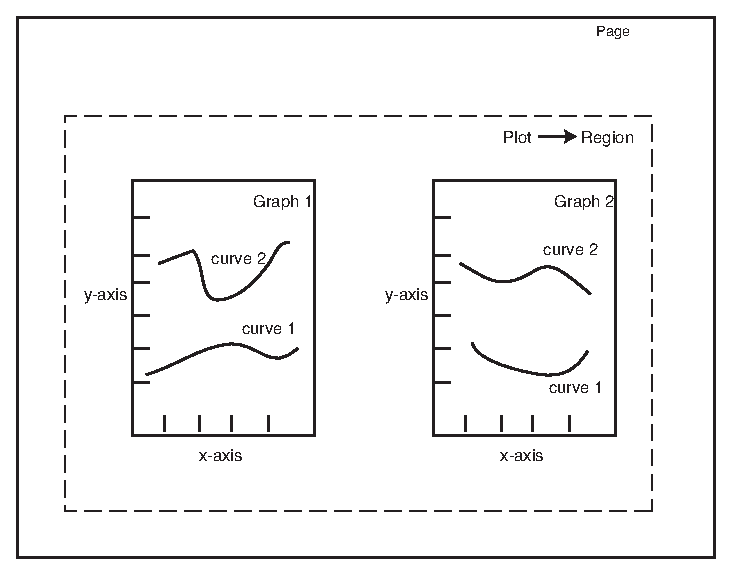
\includegraphics{plot.eps}
  \caption[A plot has a collection of graphs.]
{A plot has a collection of graphs and a graph has a 
collection of curves. A plot becomes visible when it is associated
with some region on the page using the \vn{place} command. Note that
on the actual page the plot/region border is not visible.}
  \label{f:plot}
\end{figure}

Some definitions:
  \vspace*{-3ex}
\begin{description}
\index{Curve|textbf}
\item[Curve] \Newline
A \vn{curve} is a set of (x,y) points to be plotted.
\index{Graph|textbf}
\item[Graph] \Newline
A \vn{graph} consists of horizontal and vertical axes along with a set
of \vn{curve}s that are plotted within the graph. 
\index{Plot|textbf}
\item[Plot] \Newline
A \vn{plot} is essentially a collection of \vn{graphs}.
\index{Page|textbf}
\item[Page] \Newline
The \vn{page} refers to the Xwindow where graphics are displayed or the 
corresponding printed graphics page.
\index{Region}
\item[Region] \Newline
The \vn{page} is divided up into a number of rectangles called
\vn{regions}. \vn{Regions} may overlap.
\end{description}

\index{Template plot}\index{Region}\index{Place command}
\index{Graph}\index{Plot!initialization file}\index{Curve}
The plot initialization file (cf.~Chapter~\ref{c:init}) defines a set
of \vn{template plots}. A \vn{template} defines what type of data is
to be plotted (orbit, beta function, etc.), how many \vn{graphs} there are,
what the scales are for the \vn{graph} axes, how the \vn{graph}s are
laid out, etc.  The plot initialization file also defines a set of
\vn{region}s within the \vn{page}. Any \vn{template plot} can be
placed in any region. Using the \vn{place} command (see
Chapter~\ref{c:command} for a full descriptions of all commands) one
can assign a particular \vn{template plot} to a particular region for
plotting.  The relationship between \vn{region}, \vn{plot},
\vn{graph}, and \vn{curve} is shown graphically in
Figure~\ref{f:plot}.

Figures~\ref{f:plot.page1} and \ref{f:plot.page2} show examples of a
plot \vn{page}. Figure~\ref{f:plot.page1} was generated by defining
two regions called \vn{top} and \vn{bottom} in the plot initialization
file. The \vn{top} region was defined to cover the upper half of the
\vn{page} and the \vn{bottom} region was defined to cover the bottom
half. \vn{Template plots} were defined to plot phase and orbit data
from a defined set of detector elements in the lattice. Each
\vn{template plot} defined two graphs which in both cases where
assigned the names \vn{x} and \vn{y}. The orbit \vn{template plot} was
placed in the \vn{top} region and the phase \vn{template plot} was
placed in the \vn{bottom} region. The horizontal axis numbering is by
detector \vn{index}.  Displayed plots are referred to by the
\vn{region} name (\vn{top} and \vn{bottom} in this case). Individual
graphs and curves are referred to using the nomenclature
\vn{region.graph.curve}. Thus, in this example, the horizontal orbit graph
would be referred to as \vn{top.x}.  Using the \vn{plot} command one
can then specify \vn{who} is plotted. \vn{who} refers to
\vn{measured}, \vn{reference}, \vn{model}, \vn{base}, and/or
\vn{design} data.  Notice that the same \vn{template plot} can be
assigned to different \vn{regions} and the plots in different
\vn{regions} can have different scales for their axes or different
\vn{who}. In the example in Figure~\ref{f:plot.page1}, \vn{who} for
the \vn{top} plot is \vn{model} and for the \vn{bottom} plot it is
\vn{model - design}.

Plots may be referred to by their template name or by the name of the
region they are placed in. For example, the orbit plot in
Figure~\ref{f:plot.page1} may be referred to using the region name
(\vn{top}) or the template name (\vn{orbit}). A template may be placed
in multiple regions.  For example, you may wish to plot the \vn{model}
data for the orbit in one region and the \vn{design} data for the
orbit in another region. In this case the command \vn{scale orbit}
would scale the plots in both regions while to scale the plot in only
one of the regions you would need to use the region name. A graph of a
plot is specified using the format \vn{plot_name.graph_name} where
\vn{plot_name} is a template or region name and \vn{graph_name} is the
name of the graph. For example, if the horizontal orbit graph of the
]\vn{orbit} plot is named \vn{x} then it would be referred to as
\vn{orbit.x} or \vn{top.x}. A curve within a graph is specified using
the format \vn{plot_name.graph_name.curve_name}.

The \vn{use}, \vn{veto}, \vn{restore}, and \vn{clip} commands are used
to control what data is used in fitting the model to the data in the
optimization process (see Chapter~\ref{c:opti}). The general rule is
that these commands only effect measured and reference data. If
plotting \vn{model}, \vn{design} and/or \vn{base} data then the data
will be displayed irregardless. If plotting \vn{meas} and/or \vn{ref} data
then the data displayed will vary with these commands.  \vn{meas} or
\vn{ref} data vetoed for display is also vetoed for fitting.  However,
measured data that is off the vetical or horizontal scale may still be
used by the optimizer unless vetoed with the \vn{veto} or \vn{clip}
command.  If there are data points off the vertical scale then
``**Limited**'' will appear in the upper right-hand corner of the
graph. If plotting measured data then these points off scale will
still be used by the optimizer.

The \vn{x-axis} and \vn{x-scale} commands are used to set the axis
type and scale for each graph. The axis type can be either \vn{index},
\vn{ele_index} or \vn{s} which corresponds to the data index number,
element index number and longitudinal poisition in the lattice (from
element 0) respectively.

Figure~\ref{f:plot.page2} shows another example of a plot \vn{page}.
In this case the \vn{page} was generated by again defining two
vertically stacked regions but in this case the regions have different
heights.  A \vn{template plot} with a single graph was placed in the
bottommost \vn{region}.  This \vn{graph} contains a \vn{key_table}.
A \vn{key_table} is used in conjunction with \vn{single mode} and is
explained in Chapter~\ref{c:single}. A \vn{template plot} containing
five \vn{graphs} was placed in the uppermost region. The uppermost
\vn{graph} of this \vn{template plot} contains a \vn{lat_layout} which
shows the placement of lattice elements.  What elements are displayed
in a \vn{lat_layout} and what shapes they are represented by is
specified in the initialization file. The horizontal scale is
longitudinal position (\vn{s}).  The remaining four graphs show
dispersion and beta data from two different universes representing the
low energy and high energy transport in an energy recovery linac. The
individual data points here (hard to see in this example) have been
slaved to the \vn{lat_layout} and represent the beta and dispersion at
the edges of the displayed elements in the \vn{lat_layout}.


\begin{figure}
  \centering
  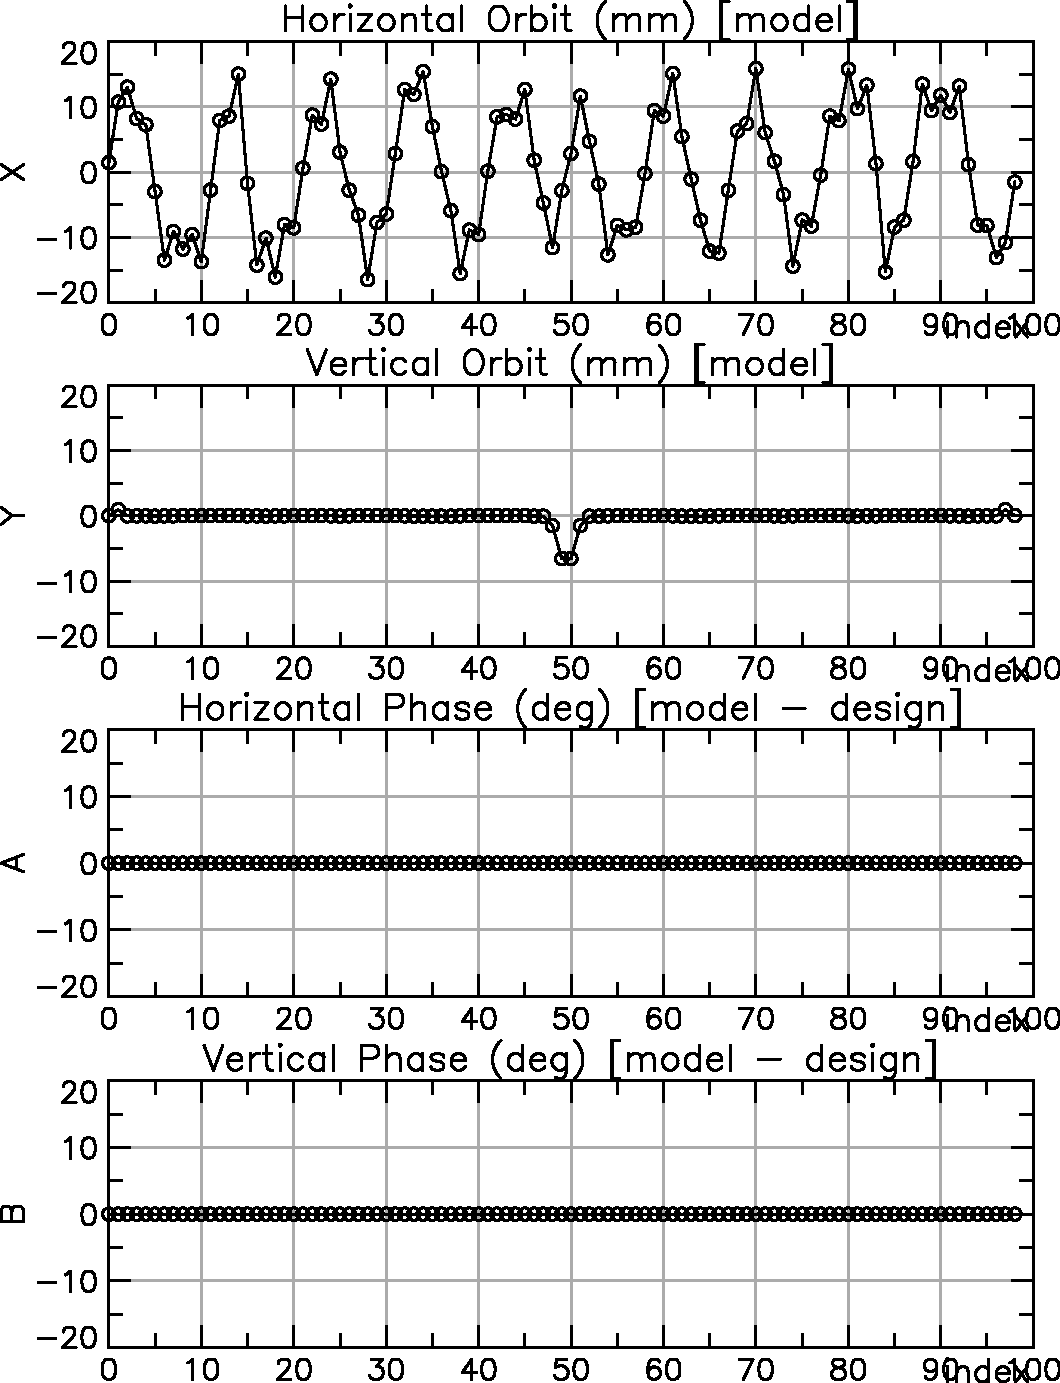
\includegraphics[width=5in]{plot-page1.eps}
  \caption{Example of a plot page}
  \label{f:plot.page1}
\end{figure}

\begin{figure}
  \centering
  \includegraphics[width=5in]{plot-page2.eps}
  \caption{Another example of a plot page.}
  \label{f:plot.page2}
\end{figure}

\vfill
\break
%------------------------------------------------------------------------
\section{Single Character Input}
\index{Single Mode}

Sometimes it is convenient to be able to vary variables using single
key strokes without having to type a carriage return.  With \tao, this
is possible using what is called \vn{single mode}. This is distinct
from \vn{line mode} where commands to \tao are typed at the command
line with a carriage return signaling the end of the command. 

The \vn{single mode} initialization file associates variables with
certain keyboard keys so that when these keys are pressed the value of
the variable is varied. This association between variables and keys is
called a \vn{key table}. See Chapter~\sref{c:single} for more details.

%------------------------------------------------------------------------
\section{Tracking Types}
\index{Tracking!Types}

\index{track_type}
\index{tao_global_struct}
\index{Global%track_type}
The are two types of tracking implemented in \tao: single particle
tracking and many particle multi-bunch tracking.
Single particle tracking is just that, the
tracking of a single particle through the lattice. Many particle
multi-bunch tracking creates a gaussian distribution of particles at
the beginning of the lattice and tracks each particle through the
lattice, including any wakefields. 
Single particle tracking is used by default. The
\vn{global%track_type} parameter (\sref{s:globals}), which is set in
the initialization file, is used to set the tracking.

Particle spin tracking has also been set up for single particle and many
particle tracking. See Sections~\sref{s:globals} and \sref{s:beam.init} for
details on setting up spin tracking.

%------------------------------------------------------------------------
\section{Lattice Calculation}\index{Lattice!calculation of}
\label{s:lat.calc}

After each \tao command is processed, the lattice and ``merit''
function are recalculated and the plot window is regenerated. The
merit function determines how well the \vn{model} fits the measured
data. See Chapter~\ref{c:opti} for more information on the merit
function and its use by the optimizer.

Below are the steps taken after each \tao command execution:
\begin{enumerate}
  \item 
The data and variables used by the optimizer is re-determined. This is
affected by commands such as \vn{use, veto,} and \vn{restore} and any
changes in the status of elements in the ring (e.g. if any elements
have been turned off).
  \item 
If changes have been made to the lattice (e.g. variables changed) then
the model lattice for all universes will be recalculated. The
\vn{model} orbit, linear transfer matrices and twiss parameters are
recalculated for every element. All data types will also be calculated
at each element specified in the initialiation file.  For single
particle tracking the linear transfer matrices and twiss parameters
are found about the tracked orbit. Tracking is
performed using the tracking method defined for each element
(i.e. Bmad Standard, Symplectic Lie, etc...). See the \bmad Reference
manual for details on tracking and finding the linear transfer
matrices and twiss parameters.
  \item 
The \vn{model} data is recalculated from the \vn{model} orbit, linear
transfer matrices, twiss parameters, particle beam information and
global lattice parameters.  Any custom data type calculations are
performed \textit{before} the standard \tao data types are calculated.
  \item 
Any user specified data post-processing is performed in
\vn{tao_hook_post_process_data}.
  \item 
The contributions to the merit function from the variables and data are
computed.
  \item 
Data and variable values are transfered to the plotting structures.
  \item 
The plotting window is regenerated.
\end{enumerate}


\chapter{Lattice File Overview}
\label{c:lat.file}
\index{lattice files|hyperbf}

\index{Bmad!lattice file format}
A lattice (\sref{c:lat.concepts}) defines the sequence of elements
that a particle will travel through along with the attributes (length,
strength, orientation, etc.) of the elements.  A lattice file (or
files) is a file that is used to describe an accelerator or storage
ring. 

%---------------------------------------------------------------------------
\section{Bmad Lattice File Format}
\label{s:lattice.file.formats}

The syntax that a \bmad standard lattice file must conform to is
modeled after the lattice input format of the \mad program.
Essentially, a \bmad lattice file is similar to a \mad lattice file
except that a \bmad file has no ``action'' commands (action commands
tell the program to calculate the Twiss parameters, do tracking,
etc.).  Since \bmad is a software library, interacting with the user
to determine what actions a program should take is left to the program
and is not part of \bmad (although the \bmad library provides the
routines to perform many of the standard calculations). A program is
not required to use the \bmad parser routines but, if it does, the
following chapters describe how to construct a valid lattice file.

%---------------------------------------------------------------------------
\section{MAD, SAD, and XSIF Lattice Files}
\label{s:mad.xsif}
\index{MAD} 
\index{XSIF}

Besides being able to parse \bmad lattice files, \bmad has software to
parse XSIF\cite{b:xsif} lattice files. See \sref{s:xsif.convert} for
more details.

While \bmad cannot directly read in \mad\cite{b:maduser} or
\vn{SAD}\cite{b:sad} files, translation between \mad and \bmad lattice
files is possible using the \vn{Universal Accelerator Parser} as
discussed in Chapter~\sref{c:lat.convert}.

%-----------------------------------------------------------------
\section{Units and Constants}
\label{s:constants}
\index{constants|hyperbf}

\bmad uses SI (Syst\'eme International) units as shown in
Table~\ref{t:units}.

\index{MAD!units}
\index{units!with MAD}
\bmad uses SI (Syst\'eme International) units as shown in
Table~\ref{t:units}.  Note that \mad uses different units. For example,
\mad's unit of Particle Energy is GeV not eV.
\begin{table}[ht]
\centering
\begin{tabular}{|l|l|} \hline
  {\em Quantity}     & {\em Units}       \\ \hline
  Angles             &    radians        \\ 
  Betatron Phase     &    radians        \\
  Current            &    Amps           \\ 
  Frequency          &    Hz             \\ 
  Kick               &    radians        \\ 
  Length             &    meters         \\ 
  Magnetic Field     &    Tesla          \\ 
  Particle Energy    &    eV             \\ 
  Phase Angles (RF)  &    radians/2$\pi$ \\ 
  Voltage            &    Volts          \\ \hline
\end{tabular}
\caption{Physical units used by \bmad.}
\label{t:units}
\end{table}

\bmad defines commonly used physical and mathematical constants
shown in Table~\ref{t:constants}.  All symbols use straight SI units
except for \vn{emass} and \vn{pmass} which are provided for
compatibility with \mad.

\begin{table}
\centering
\begin{tabular}{|l|l|l|l|} \hline
  {\em Symbol}    & {\em Value}       & {\em Units}     &  {\em Name}           \\ \hline
  pi              & 3.14159265359          &            &                       \\
  twopi           & 2 * pi                 &            &                       \\
  fourpi          & 4 * pi                 &            &                       \\
  e_log           & 2.718281828            &            &                       \\
  sqrt_2          & 1.4142135623731        &            &                       \\
  degrad          & 180 / pi               &            & From rad to deg       \\
  degrees         & pi / 180               &            & From deg to rad       \\
  raddeg          & pi / 180               &            & From deg to rad       \\
  m_electron      & $0.51099906 \pow{6}$   & eV         & Electron mass         \\
  m_muon          & $105.6583715 \pow{6}$  & eV         & Muon mass             \\
  m_pion_0        & $134.9766 \pow{6}$     & eV         & $\pi^0$ mass          \\
  m_pion_charged  & $139.57018 \pow{6}$    & eV         & $\pi^+$, $\pi^-$ mass \\
  m_proton        & $0.938271998 \pow{9}$  & eV         & Proton mass           \\
  c_light         & $2.99792458 \pow{8}$   & m/sec      & Speed of light        \\
  r_e             & $2.8179380 \pow{-15}$  & m          & Electron radius       \\
  r_p             & $1.5346980 \pow{-18}$  & m          & Proton radius         \\
  e_charge        & $1.6021892 \pow{-19}$  & Coul       & Electron charge       \\
  h_planck        & $4.13566733 \pow{-15}$ & eV*sec     & Planck's constant     \\
  h_bar_planck    & $6.58211899 \pow{-16}$ & eV*sec     & Planck / $2\pi$       \\
  emass           & $0.51099906 \pow{-3}$  & GeV        & Electron mass         \\
  pmass           & $0.938271998$          & GeV        & Proton mass           \\ \hline
\end{tabular}
\caption{Physical and mathematical constants recognized by \bmad.}
\label{t:constants}
\end{table}

%---------------------------------------------------------------------------
\section{File Example and Syntax}
\index{Bmad!statement syntax}

\index{parameter statement}
\index{use statement}
The following (rather silly) example shows some of the features of a
\bmad lattice file:
\begin{example}
  ! This is a comment
  parameter[E_TOT] = 5e9                   ! Parameter definition
  pa1 = sin(3.47 * pi / c_light)                 ! Constant definition
  bend1: sbend, type = "arc bend", l = 2.3,      ! An element definition
      g = 2*pa1, tracking_method = bmad_standard
  bend2: bend1, l = 3.4                          ! Another element def
  bend2[g] = 105 - exp(2.3) / 37.5               ! Redefining an attribute
  ln1: line = (ele1, ele2, ele3)                 ! A line definition
  ln2: line = (ln1, ele4, ele5)                  ! Lines can contain lines
  arg_ln(a, b) = (ele1, a, ele2, b)              ! A line with arguments.
  use, ln2                                       ! Which line to use for the lattice
\end{example}

\index{"! comment symbol}
\index{comment symbol ("!)}
A \bmad lattice file consists of a sequence of statements. An
exclamation mark (!) denotes a comment and the exclamation mark and
everything after the exclamation mark on a line are ignored.  \bmad is
generally case insensitive. Most names are converted to
uppercase. Exceptions where a name is not converted include file names
and atomic formulas for materials used in crystal diffraction.

\index{\& continuation symbol}
\index{continuation symbol (\&)}
Normally a statement occupies a single line in the file. Several
statements may be placed on the same line by inserting a semicolon
(``;'') between them. A long statement can occupy multiple lines by
putting an ampersand (``\&'') at the end of each line of the statement
except for the last line. Additionally, lines that end with an
``implicit continuation character''
are automatically continued to the next line. The implicit continuation 
characters are
\begin{example}
  ,   (   \{   [   =
\end{example}
Notice
that this is {\em not} like \vn{C/C++}. Thus the following is bad syntax
\begin{example}
  wall = \{
    section = \{s = 0.45     ! BAD SYNTAX. NO CONTINUATION CHARACTER HERE.
    \}                       ! BAD SYNTAX. NO CONTINUATION CHARACTER HERE.
  \}
\end{example}
Correct is:
\begin{example}
  wall = \{
    section = \{s = 0.45\} \}
\end{example}
or even:
\begin{example}
  wall = \{
    section = \{s = 0.45\} \&
  \}
\end{example}

\index{lattice files!name syntax}
Names of constants, elements, lines, etc. are limited to 40
characters. The first character must be a letter (\vn{A} --- \vn{Z}).
The other characters may be a letter, a digit (\vn{0} --- \vn{9}) or
an underscore (\vn{_}). Other characters may appear but should be avoided
since they are used by Bmad for various purposes. For example, the 
backslash (\vn{\B}) character is used to by Bmad when forming the names of
superposition slaves (\sref{s:super}) and dots (\vn{.}) are used by Bmad 
when creating names of \vn{tagged} elements (\sref{s:tag}). Also use of
special characters may make the lattice files less portable to non-Bmad programs.

\index{parameter statement}
\index{parameter statement}
\index{parameter statement}
\index{beginning statement}
The following example constructs a linear lattice with two elements: 
\begin{example}
  parameter[geometry] = LINEAR_LATTICE
  parameter[e_tot] =2.7389062E9
  parameter[particle] = POSITRON
  beginning[beta_a] = 14.5011548
  beginning[alpha_a] = -0.53828197
  beginning[beta_b] = 31.3178048
  beginning[alpha_b] = 0.25761815
  q: quadrupole, l = 0.6, b1_gradient = 9.011
  d: drift, l = 2.5
  t: line = (q, d)
  use, t 
\end{example}
here \vn{parameter[geometry]} (\sref{s:param}) is set to \vn{LINEAR_LATTICE}
which specifies that the lattice is not circular. In this case, the beginning 
Twiss parameters need to be specified and this is done by the \vn{beginning}
statements (\sref{s:beginning}). A quadrupole named \vn{q}
and a drift element named \vn{d} are specified
and the entire lattice consists of element \vn{q} followed by element \vn{d}.

%----------------------------------------------------------------------------
\section{Digested Files}
\label{s:digested}
\index{digested files}

Normally the \bmad parser routine will create what is called a
``digested file'' after it has parsed a lattice file so that when a
program is run and the same lattice file is to be read in again, to save
time, the digested file can be used to load in the lattice information.
This digested file is in binary format and is not human readable. The
digested file will contain the transfer maps for all the elements. 
Using a digested file can save considerable time if some of the
elements in the lattice need to have Taylor maps computed.
(this occurs typically with map--type wigglers).

\bmad creates the digested file in the same area as the lattice file.
If \bmad is not able to create a digested file (typically because it
does not have write permission in the directory), an error message will
be generated but otherwise program operation will be normal.

\index{ran}
\index{ran_gauss}
Digested files contain the names of the lattice files used to create
them. If a lattice file has been modified since the digested file has
been created then the lattice files will be reread and a new
digested file will be generated. 

Note: If any of the random number functions (\sref{s:functions}) are
used in the process of creating the lattice, the digested file will be
ignored. In this case, each time the lattice is read into a program,
different random numbers will be generated for expressions that use such
random numbers.

Digested files can also be used for easy transport of lattices between
programs or between sessions of a program. For example, using one
program you might read in a lattice, make some adjustments (say to model
shifts in magnet positions) and then write out a digested version of the
lattice. This adjusted lattice can now be read in by another program.

%---------------------------------------------------------------------------
\section{Element Sequence Definition}

\index{line}\index{use statement|hyperbf}
A \vn{line} defines a sequence of elements. \vn{lines} may contain
other \vn{lines} and so a hierarchy may be established. One line is
selected, via a \vn{use} statement, that defines the lattice. For
example:
\begin{example}
  l3: line = (l1, l2)   ! Concatenate two lines
  l1: line = (a, b, c)  ! Line with 3 elements
  l2: line = (a, z)     ! Another line 
  use, l3               ! Use l3 as the lattice definition.
\end{example}
In this case the lattice would be
\begin{example}
  (a, b, c, a, z)
\end{example}
\vn{Lines} can be defined in any order. See \cref{c:sequence} for more
details.

\index{superimpose}
The \vn{superimpose} construct allows elements to be placed in a
lattice at a definite longitudinal position. What happens is that
after a lattice is expanded, there is a reshuffling of the elements to
accommodate any new superimpose elements. See \sref{s:super} for more
details.

%---------------------------------------------------------------------------
\section{Lattice Elements}

The syntax for defining a lattice element roughly follows the
\mad\cite{b:maduser} program:
\begin{example}
  ele_name: keyword [, attributes]
\end{example}
where \vn{ele_name} is the element name, \vn{keyword} is the type of
element, and \vn{attributes} is a list of the elements
attributes. \cref{c:elements} gives a list of elements types with
their attributes.
\vn{Overlay} and \vn{group} type elements have a slightly different syntax:
\begin{example}
  ele_name: keyword = \{ list \}, master-attribute [= value] [, attributes]
\end{example}
and \vn{Girder} elements have the syntax
\begin{example}
  ele_name: keyword = \{ list \} [, attributes]
\end{example}  
For example:
\begin{example}
  q01w: quadrupole, type = "A String", l = 0.6, tilt = pi/2
  h10e: overlay = \{ b08e, b10e \}, var = \{hkick\}
\end{example}

%---------------------------------------------------------------------------
\section{Lattice Element Names}
\label{s:ele.names}
\index{element!names}

\index{element!name}\index{superimpose}\index{multipass}
A valid element name may be up to 40 characters in length. The first
character of the name must be a letter [A-Z]. After that, the rest of
the name can contain only letters, digits [0-9], underscore ``_'',
period ``.'', backslash ``\B'', or a hash mark ``\#''. It is best to
avoid these last three symbols since \bmad uses them to denote
``relationships''.  Periods are used for tagging (\sref{s:tag}), and
backslash and hash marks are used for to compose names for
superposition (\sref{s:super}) and multipass (\sref{s:multipass})
slave elements.

\index{reserved names}
\index{beam}\index{beam_start}\index{beginning}
\index{end}\index{parameter}\index{root}
There is a short list of names that cannot be used as an element name. 
These reserved names are:
\begin{example}
  beam
  beam_start
  beginning
  end
  parameter
  root
\end{example}

Where appropriate, for example when setting element attributes
(\sref{s:lat.attribs}), the wildcards \vn{``*''} and \vn{``%''} can be
used to select multiple elements.  The \vn{``*''} character will match
any number of characters (including zero) while \vn{``%''} maches to
any single character. Additionally, matching can be restricted to a
certain element class using the syntax:
\begin{example}
  class::element_name
\end{example}
where \vn{class} is a class name. For example:
\begin{example}
  m*              ! Match to all elements whose name begins with "m".
  a%c             ! Match to "abc" but not to "ac" or "azzc".
  quadrupole::*w  ! Match to all quadrupoles whose name ends in "w"
\end{example}

After lattice expansion (\sref{s:expand}), the general syntax to
specify a set of elements is:
\begin{example}
  \{class::\}\{branch_id>>\}element_id\{##N\}
\end{example}
where \vn{\{...\}} markes an optional component, \vn{class} is a class
name, \vn{branch_id} is a branch name or index (\sref{s:branch.def}),
\vn{element_id} is and element name or element index
(\sref{s:lines.wo.arg}), and \vn{\#\#N} indicates that the N\Th matching
element is to be used. Examples:
\begin{example}
  quad::x_br>>q*        ! All quadrupoles of branch "x_br" whose name begins with "q".
  2>>45                 ! element \#45 of branch \#2.
  q01##3                ! The 3rd element in each branch named q01.
\end{example}

Multiple elements in a lattice may share the same name.  When
multiple branches are present, to differentiate elements that
appear in different branches, the ``branch qualified'' element name may be
used. The branch qualified element name is of the form
\begin{example}
  branch_name>>element_name
\end{example}
where \vn{branch_name} is the name of the branch and \vn{element_name}
is the ``regular'' name of the element. Example:
\begin{example}
  root>>q10w
  x_branch>>crystal3
\end{example}

For \vn{branch} lines (\sref{s:branch.def}), the full ``branch
qualified'' name of an element is of the form
\begin{example}
  branch_name>>element_name
\end{example}
where \vn{branch_name} is the name of the branch and \vn{element_name} is the
``regular'' name of the element. Example:
\begin{example}
  root>>q10w
  xline>>cryst3
\end{example}
Using the full name is only needed to distinguish elements that have
the same regular name in separate branches.  When parsing a lattice
file, branches are not formed until the lattice is expanded
(\sref{s:expand}). Therefore an \vn{expand_lattice} statement is
required before full names can be used in statements.

%---------------------------------------------------------------------------
\section{Lattice Element Attributes}
\label{s:lat.attribs}
\index{element attributes|hyperbf}

Any lattice element has various attributes like its name, its length,
its strength, etc. The values of element attributes can be
specified when the element is defined. For example:
\begin{example}
  b01w: sbend, l = 6.0, rho = 89.0 ! Define an element with attributes.
\end{example}
After an element's definition, an individual attribute may be referred
to using the syntax
\begin{example}
  class::element_name[attribute_name]
\end{example}
Element attributes can be set or used in an algebraic expression:
\begin{example}
  bo1w[roll] = 6.5                  ! Set an attribute value.
  b01w[l] = 6.5                     ! Change an attribute value.
  b01w[l] = b01w[rho] / 12          ! OK to reset an attribute value.
  my_const = b01w[rho] / b01w[l]    ! Use of attribute values in an expression.
\end{example}
Notice that there can be no space between the element name and the
\vn{[} opening bracket.  

Chapter \cref{c:elements} lists the attributes appropriate for each
element class.

When setting an attribute value, if more than one element has the
\vn{element_name} then {\it all} such elements will be set. When
setting an attribute value, if \vn{element_name} is the name of a type
of element, all elements of that type will be set. For example
\begin{example}
  q_arc[k1] = 0.234                      ! Set all elements named Q_ARC. 
  rfcavity::*[voltage] = 3.7             ! Set all RFcavity elements.
\end{example}


A prepended plus sign ``+'' indicates that if no elements are matched to, this
is not an error. For example
\begin{example}
  +sextupole::*[tracking_method] = taylor
\end{example}
In this case, it is not an error if there are no sextupoles in the lattice.

The wild cards \vn{``*''}, and \vn{``\%''} can be used to can be used
(\sref{s:ele.names}). Examples:
\begin{example}
  *[tracking_method] = bmad_standard  ! Matches all elements.
  quadrupole::Q*[k1] = 0.234    ! Matches all quadrupoles with names beginning with Q.
  Q%1[k1] = 0.234               ! Matches to "Q01" but not "Q001".
\end{example}
\index{beginning element}
Note: A name with wild cards will never match to the \vn{BEGINNING} element (\sref{s:use}).

After lattice expansion (\sref{s:expand}), the attributes of specific elements
may be set using the syntax as discussed in Section \sref{s:ele.names}. Example:
\begin{example}
  expand_lattice              ! Expand the lattice.
  97[x_offset] = 0.0023       ! Set x_offset attribute of 97th element
  b2>>si_cryst##2[tilt] = 0.1 ! Tilt the 2nd instance of "si_cryst" in branch "b2" 
\end{example}

%---------------------------------------------------------------------------
\section{Custom Element Attribute Names}
\label{s:custom.attrib}
\index{element attributes!defining custom attributes}

Real scaler custom element attributes may be defined for any class of
element.  Custom element attributes are useful with programs that need
to associate ``extra'' information with particular lattice elements
and it is desired that this extra information be settable from within
a lattice file. For example, a program might need error tollerances
for the strength of quadrupoles.

Adding custom attributes will not disrupt programs that are not
designed to use the custom attributes. Currently, up to five custom
attributes may be defined for any given element type. The syntax for
defining custom attributes is:
\begin{example}
  parameter[custom_attributeN] = "\{class::\}attribute_name"
\end{example}
\vn{custom_attributeN} may be one of:
\begin{example}
  custom_attribute1
  ...
  custom_attribute5
\end{example}
and "\vn{attribute_name}" is the name of the attribute. To restrict the
custom attribute to a particular element class, the element class
can be prefixed to the attribute name. Examples:
\begin{example}
  parameter[custom_attribute1] = "mag_id"
  parameter[custom_attribute1] = "quadrupole::error_k1"
  parameter[custom_attribute2] = "color"
\end{example}
The first line in the example assigns a custom attributge name of
\vn{mag_id} to all elements.  The second line in the example overrides
the setting of \vn{custom_attribute1} for quadrupole elements only. 

Once a custom attribute has been defined it may be set for an element
of the correct type. Example:
\begin{example}
  parameter[custom_attribute2] = "lcavity::rms_phase_err"
  ...
  l2a: lcavity, rms_phase_err = 0.0034, ...
\end{example}

For someone creating a program, section~\sref{s:ele.gen} describes how
to make the appropriate associations.

Note: If custom string information needs to be associated with an
element, the \vn{type}, \vn{alias} and \vn{descrip} element components
(\sref{s:alias}) are available.

%---------------------------------------------------------------------------
\section{Variable Types}
\label{s:var.types}
\index{arithmetic expressions!variables}

\index{logicals|hyperbf}
There are five types of variables in \bmad: reals, integers, switches,
logicals (booleans), and strings. Acceptable logical values are
\begin{example}
   true    false
   t       f
\end{example}
For example
\begin{example}
  rf1[is_on] = False
\end{example}

\index{strings|hyperbf}
String literals can be quoted using double quotes (") or single quotes ('). 
If there are no
blanks or commas within a string, the quotes can be omitted. For example:
\begin{example}
  Q00W: Quad, type = "My Type", alias = Who_knows, &
                                  descrip = "Only the shadow knows"
\end{example}
Unlike most everything else, strings are not converted to uppercase.

\index{switches|hyperbf}
Switches are variables that take discrete values. For example:
\begin{example}
  parameter[particle] = positron          
  q01w: quad, tracking_method = bmad_standard 
\end{example}
The name ``switch'' can refer to the variable (for example,
\vn{tracking_method}) or to a value that it can take (for example,
\vn{bmad_standard}). The name ``method'' is used interchangeably with switch.

%---------------------------------------------------------------------------
\section{Arithmetic Expressions}
\index{arithmetic expressions} 
\label{arithmetic}

Arithmetic expressions can be used in a place where a real value is required.
The standard operators are defined: \hfil\break
\hspace*{0.15in}
\begin{tabular}{ll}
  $a + b$           & Addition        \\
  $a - b$           & Subtraction     \\
  $a \, \ast \, b$  & Multiplication  \\
  $a \; / \; b$     & Division        \\
  $a \, \land \, b$ & Exponentiation  \\
\end{tabular}
\hfil\break
\bmad also has a set of intrinsic functions. A list of these is given
in \sref{s:functions}.

\index{arithmetic expressions!constants}
Literal constants can be entered with or without a decimal point. An
exponent is marked with the letter E. For example
\begin{example}
  1, 10.35, 5E3, 314.159E-2
\end{example}
Symbolic constants can be defined using the syntax
\begin{example}
  parameter_name = expression
\end{example}
\index{MAD!syntax compatibility with BMAD}
Alternatively, to be compatible with \mad, using ``:='' instead of ``='' is accepted
\begin{example}
  parameter_name := expression
\end{example}
Examples:
\begin{example}
  my_const = sqrt(10.3) * pi^3
  abc     := my_const * 23
\end{example}
\index{MAD!delayed substitution}
Unlike \mad, \bmad uses immediate substitution so that all constants
in an expression must have been previously defined. For example, the
following is {\em not} valid:
\begin{example}
  abc      = my_const * 23      ! No: my_const needs to be defined first.
  my_const = sqrt(10.3) * pi^3
\end{example}
here the value of \vn{my_const} is not known when the line ``\vn{abc}
= $\ldots$'' is parsed. Once
defined, symbolic constants cannot be redefined. For example:
\begin{example}
  my_const = 1
  my_const = 2  ! No: my_const cannot be redefined.
\end{example}

Element attributes can be used after they have been defined but not
before.  Example:
\begin{example}
  sa: sextupole, l = 0.3, k2 = 0.01 * sa[l]  ! Good
  sb: sextupole, k2 = 0.01 * sb[l], l = 0.3  ! BAD SET OF K2!
\end{example}
In this example, the \vn{k2} attribute of element \vn{sa} is correctly
set since \vn{k2} is defined after \vn{l}. On the other hand, \vn{k2}
of element \vn{sb} will have a value of zero since \vn{l} of \vn{sb}
defaults to zero before it is set.

Another potential pitfall with immediate substitution is when using
dependent element attributes (\sref{s:depend}). For example:
\begin{example}
  b01w: sbend, l = 0.5, angle = 0.02
  a_const = b01w[g]    ! No: bend g has not yet been computed!
\end{example}
Here the bend strength \vn{g} (\sref{s:bend}) will eventually be
computed to be 0.04 (= angle / l) but that computation does not happen
until lattice expansion (\sref{s:expand}). In this case, the value of
\vn{a_const} will be the default value of \vn{g} which is zero.  As a
rule of thumb, never rely on dependent attributes having their correct
value.

%---------------------------------------------------------------------------
\section{Intrinsic functions}
\label{s:functions}
\index{intrinsic functions}

\index{sqrt}\index{log}\index{exp}\index{sin}\index{cos}\index{tan}\index{factorial}
\index{asin}\index{acos}\index{atan}\index{abs}\index{ran}\index{ran_gauss}
The following intrinsic functions are recognized by \bmad: \hfil\break
\hspace*{0.15in}
\begin{tabular}{ll}
  \vn{sqrt}(x)      & Square Root                        \\
  \vn{log}(x)       & Logarithm                          \\
  \vn{exp}(x)       & Exponential                        \\
  \vn{sin}(x)       & Sine                               \\
  \vn{cos}(x)       & Cosine                             \\
  \vn{tan}(x)       & Tangent                            \\
  \vn{asin}(x)      & Arc sine                           \\
  \vn{acos}(x)      & Arc cosine                         \\
  \vn{atan}(x)      & Arc Tangent                        \\
  \vn{atan2}(y, x)  & Arc Tangent of y/x                 \\
  \vn{abs}(x)       & Absolute Value                     \\
  \vn{factorial}(n) & Factorial                          \\
  \vn{ran}()        & Random number between 0 and 1      \\
  \vn{ran_gauss}()  & Gaussian distributed random number \\
  \vn{int}(x)       & Nearest integer with magnitude less then x \\
  \vn{nint}(x)      & Nearest integer to x               \\
  \vn{floor}(x)     & Nearest integer less than x        \\
  \vn{ceiling}(x)   & Nearest integer greater than x     \\
\end{tabular}

\index{ran_seed}
\vn{ran_gauss} is a Gaussian distributed random number with unit RMS. 
Both \vn{ran} and \vn{ran_gauss} use a seeded random number generator. 
To choose the seed set 
\begin{example}
  parameter[ran_seed] = <Integer>
\end{example}
A \vn{value} of zero will set the seed using the system clock so that
different sequences of random numbers will be generated each time a
program is run.  The default behavior if \vn{parameter[ran_seed]} is
not present is to use the system clock for the seed.

\index{expand_lattice}
If an element is used multiple times in a lattice, and if \vn{ran} or
\vn{gauss_ran} is used to set an attribute value of this element, then
to have all instances of the element have different attribute values
the setting of the attribute must be after the lattice has been
expanded (\sref{s:expand}). For example:
\begin{example}
  a: quad 
  a[x_offset] = 0.001*ran_gauss()
  my_line: line = (a, a)
  use, my_line
\end{example}
Here, because \bmad does immediate evaluation, the \vn{x_offset}
values for \vn{a} gets set in line 2 and so both copies of \vn{a} in
the lattice get the same value. This is probably not what is wanted.
On the other hand if the attribute is set after lattice expansion:
\begin{example}
  a: quad 
  my_line: line = (a, a)
  use, my_line
  expand_lattice
  a[x_offset] = 0.001*ran_gauss()
\end{example}
Here the two \vn{a} elements in the lattice get different values for
\vn{x_offset}.

%-----------------------------------------------------------------------------
\section{Print Statement}
\label{s:print}
\index{print statement|hyperbf}

The \vn{print} statement prints a message at the terminal when the 
lattice file is parsed by a program. Syntax:
\begin{example}
  print <String>
\end{example}
For example
\begin{example}
  print Remember! Q01 quad strength not yet optimized!
\end{example}
The \vn{print} statement is useful to remind someone using the lattice of important details.

%-----------------------------------------------------------------------------
\section{Title Statement}
\index{title statement|hyperbf}

The \vn{title} statement sets a title string which can be used by a program. 
For consistency with \mad there are two possible syntaxes
\begin{example}
  title, <String>
\end{example}
or the statement can be split into two lines
\begin{example}
  title
  <String>
\end{example}
For example
\begin{example}
  title
  "This is a title"
\end{example}

%--------------------------------------------------------------------------
\section{Call Statement}
\label{s:call}
\index{call statement|hyperbf}

It is frequently convenient to separate the lattice definition into
several files.  Typically there might be a file (or files) that define
the layout of the lattice (something that doesn't change often) and a
file (or files) that define magnet strengths (something that changes
more often).  The \vn{call} is used to read in separated lattice
files. The syntax is
\begin{example}
  call, filename = <String>
\end{example}
Example:
\begin{example}
  call, filename = "../layout/my_layout.bmad"      ! Relative pathname
  call, filename = "/nfs/cesr/lat/my_layout.bmad"  ! Absolute pathname
\end{example}
\bmad will read the called file until a \vn{return} or \vn{end_file}
statement is encountered or the end of the file is reached.

For filenames that are relative, the called file will be searched for in
two different locations:
\begin{example}
  1) Relative to the directory of the calling file.
  2) Relative to the current directory.
\end{example}
The first instance where a file is found is used.
Thus, in the above example, the first call will search for:
\begin{example}
  1) ../layout/my_layout.bmad  (relative to the calling file directory)
  2) ../layout/my_layout.bmad  (relative to the current directory)
\end{example}

An XSIF (\sref{s:lattice.file.formats}) lattice file may be called
from within a \bmad lattice file by prepending \vn{"xsif::"} to the
file name. Example:
\begin{example}
  call, filename = "xsif::my_lattice.xsif"
\end{example}
This statement must be the first statement in the \bmad lattice file
except for any comments or debugging statements (\sref{s:debug}). 
The XSIF lattice file must define a
complete lattice and cannot contain any \bmad specific statements. The
call to the XSIF file automatically expands the lattice
(\sref{s:expand}) and any additional statements in the \bmad lattice
file operate on the expanded lattice.

%--------------------------------------------------------------------------
\section{Inline Call}
\label{s:call.inline}
\index{call!inline}

Any lattice elements will have a set of attributes that need to be defined.
As a convenience, it is possible to segregate an element attribute or attributes
into a separate file and then ``call'' this file using an
``inline call''. The inline call has three forms. In an element definition,
the inline call has the form
\begin{example}
  <ele_name>: <ele_type>, ..., call::<file_name>, ...
\end{example}
or
\begin{example}
  <ele_name>: <ele_type>, ..., <attribute_name> = call::<file_name>, ...
\end{example}
where \vn{<attribute_name>} is the name of the attribute and
\vn{<file_name>} is the name of the where the attribute structure is
given.  The third form of the inline call occurs when an element
attribute is redefined and has the form
\begin{example}
  <ele_name>[<attribute_name>] = call::<file_name>
\end{example}
Example:
\begin{example}
  c: crystal, call::my_curvature.bmad, surface = call::my_surface.bmad, ...
\end{example}  


%--------------------------------------------------------------------------
\section{Return and End_File statements}
\index{return statement|hyperbf}
\index{end_file statement|hyperbf}

\vn{Return} and \vn{end_file} have identical effect and tell \bmad to
ignore anything beyond the \vn{return} or \vn{end_file} statement in
the file.

%----------------------------------------------------------------------------
\section{Expand_Lattice Statement}
\label{s:expand}
\index{lattice!expansion|hyperbf}
\index{expand_lattice|hyperbf}

At some point in parsing a lattice file, the ordered sequence (or
sequences if there are multiple branches) of elements that form a
lattice must be constructed. This process is called \vn{lattice
expansion} since the element sequence can be built up from
sub--sequences (\sref{c:sequence}). Normally, lattice expansion
happens automatically at the end of the parsing of the lattice file
but an explicit \vn{expand_lattice} statement in a lattice file will
cause immediate expansion. The reason why this can be important is
that there are restrictions, on some types of operations which must
come either before or after lattice expansion:
\begin{Itemize}
\item 
\index{ran}
\index{ran_gauss}
The \vn{ran} and \rn{ran_gauss} functions, when used with elements
that show up multiple times in a lattice, generally need to be used
after lattice expansion. See \sref{s:functions}.
\item
\index{line}\index{list}\index{use}
All \vn{line}s (\sref{s:lines.wo.arg}), \vn{list}s
(\sref{s:replace.list}), and \vn{use} (\sref{s:use}) statements must
come before lattice expansion.
\item
Some dependent variables may be set as if they are independent
variables but only if done before lattice expansion. See \sref{s:depend}.
\index{multipass}
\item 
Setting the \vn{phi0_multipass} attribute for an 
\vn{Lcavity} or \vn{RFcavity} multipass
slave may only be done after lattice expansion (\sref{s:multipass}).
\item
\index{tags for Lines and Lists}
Setting individual element attributes for tagged elements can only be done
after lattice expansion (\sref{s:tag}).
\end{Itemize}

Lattice expansion is only done once so it is an error if multiple
\vn{expand_lattice} statements are present.

\index{secondary lattice file}
A lattice file where all the statements are post lattice expansion
valid is called a ``\vn{secondary lattice file}''.  To promote
flexibility, \bmad has methods for parsing lattices in a two step
process: First, a ``primary'' lattice file that defines the basic
lattice is read. After the promary lattice has been parsed and lattice
expansion has been done, the second step is to read in one or more
secondary lattice files. Such secondary lattice files can be used, for
example, to set such things as element misalignments. The point here
is that there are no calls (\sref{s:call}) of the secondary files in
the primary file so the primary lattice file does not have to get
modified when different secondary files are to be used.

%--------------------------------------------------------------------------
\section{Debugging Statements}
\label{s:debug}
\index{no_digested statement}
\index{no_superimpose statement}
\index{parser_debug statement}
\index{debug_marker statement}
\index{no_digested statement}
\index{lattice files!parser debugging}

There are a few statements
which can help in debugging the \bmad lattice parser
itself. That is, these statements are generally only used by programmers.
These statements are:
\begin{example}
  debug_marker
  no_digested
  no_superimpose
  parser_debug
\end{example}

The \vn{debug_marker} statement is used for marking a place in the lattice file
where program execution is to be halted. This only works when running
a program in conjunction with a program debugging tool. 

The \vn{no_digested} statement if present, will prevent \bmad from 
creating a digested file (\sref{s:digested}. That is, the lattice file will always
be parsed when a program is run.

The \vn{no_superimpose} statement is used to suppress superpositions
(\sref{s:super}). This is useful for debugging purposes.

The \vn{parser_debug} statement will cause information about the
lattice to be printed out at the terminal. It is recommended that this
statement be used with small test lattices since it can generate a lot
of output. The syntax is
\begin{example}
  parser_debug <switches>
\end{example}
Valid \vn{<switches>} are
\begin{example}
  beam_start          ! Print the beam_start information.
  ele <n1> <n2> ...   ! Print full info on selected elements.
  lattice             ! Print a list of lattice element information.
  lord                ! Print full information on all lord elements.
  seq                 ! Print sequence information.
  slave               ! Print full information on all slave elements.
  var                 ! Print variable information.
\end{example}
Here $<n1>$, $<n2>$, etc. are the index of the selected elements in
the lattice.  Example
\begin{example}
  parser_debug var lat ele 34 78
\end{example}


\chapter{Elements}

A lattice for a storage ring or linac is made up of a collection of
elements --- Quadrupoles, Bends, etc. This chapter discusses the
various types of elements available in \bmad.

\section{Bmad Elements}

Most element types available in \mad\ are provided in \bmad.
Additionally, \bmad\ provides a number of element types that are not
available in \mad.  A word of caution: In some cases where both \mad\
and \bmad\ provide the same element type, there will be an overlap of 
the attributes available but the two sets of attributes will not be the same.
The list of element types known to \bmad\ is shown in Table~\ref{tab:elements}.
In
\begin{table}[h]
{\centering
{\tt
\begin{tabular}{|l|l||l|l|} \hline
  {\it Element} & {\it Section}     & {\it Element} & {\it Section} \\ \hline
  ab\_multipole & \ref{s:ab_m}      &  octupole     & \ref{s:oct}   \\ \hline
  accel\_sol    & \ref{s:accel_sol} &  overlay      & \ref{s:over}  \\ \hline
  beambeam      & \ref{s:bbi}       &  patch        & \ref{s:patch} \\ \hline
  custom        & \ref{s:custom}    &  quadrupole   & \ref{s:quad}  \\ \hline
  drift         & \ref{s:drift}     &  rbend        & \ref{s:rbend} \\ \hline
  ecollimator   & \ref{s:col}       &  rcollimator  & \ref{s:col}   \\ \hline
  elseparator   & \ref{s:elsep}     &  rfcavity     & \ref{s:rfcav} \\ \hline
  group         & \ref{s:group}     &  sbend        & \ref{s:sbend} \\ \hline
  hkicker       & \ref{s:kicker}    &  sextupole    & \ref{s:sex}   \\ \hline
  instument     & \ref{s:mon}       &  solenoid     & \ref{s:sol}   \\ \hline
  kicker        & \ref{s:kicker}    &  sol\_quad    & \ref{s:sq}    \\ \hline
  lcavity       & \ref{s:lcav}      &  taylor       & \ref{s:tay}   \\ \hline
  marker        & \ref{s:mark}      &  vkicker      & \ref{s:kicker}\\ \hline
  monitor       & \ref{s:mon}       &  wiggler      & \ref{s:wig}   \\ \hline
  multipole     & \ref{s:m}         &               &               \\ \hline  
\end{tabular}
}}
\caption{\bmad\ elements.}
\label{tab:elements}\center
\end{table}

\vfil
\break

%-----------------------------------------------------------------
\section{AB\_Multipole}
\label{s:ab_m}

An \vn{AB_Multipole} is a thin multipole lens up to 20th order. The only
difference between this and a \vn{Multipole} is the input format. See the 
Magnetic fields section \ref{s:fields} for more details.

\begin{table}[h]
{\centering 
{\tt
\begin{tabular}{|l|l||l|l||l|l|} \hline
  {\sl Attribute} & {\sl Sec}  & {\sl Attribute} & {\sl Sec} & {\sl Attribute} & {\sl Sec} \\ \hline
  a$n$, b$n$ = Real  &  \ref{s:ab}     &  type = String                & \ref{s:string} & x\_limit = Real  & \ref{s:limit} \\ \hline
  tilt       = Real  &  \ref{s:offset} &  alias = String               & \ref{s:string} & y\_limit = Real  & \ref{s:limit} \\ \hline
  x\_offset  = Real  &  \ref{s:offset} &  descrip = String             & \ref{s:string} & aperture = Real  & \ref{s:limit} \\ \hline
  y\_offset  = Real  &  \ref{s:offset} &  mat6\_calc\_method = Switch  & \ref{s:track}  & is\_on = Logical & \ref{s:is_on} \\ \hline
  s\_offset  = Real  &  \ref{s:offset} &  tracking\_method = Switch    & \ref{s:track}  &                  &               \\ \hline
\end{tabular}
}}
\end{table}

\noindent
Possible \vn{mat6_calc_method} and \vn{tracking_method} values are:
\vskip 0.01in
\begin{example}
   bmad\_standard  (default) 
\end{example}

\vskip0.2in \noindent
Example:
\begin{example}
  abc: ab_multipole, a2 = 0.034e-2, b3 = 5.7e-4
\end{example}

\vskip0.1in \noindent
Dependent attributes:
\begin{example}
  beam\_energy  ! See section \ref{s:energy}
\end{example}

%-----------------------------------------------------------------
\section{Accel\_Sol}
\label{s:accel_sol}

An \vn{Accel_Sol} element is a combination LINAC RF accelerating
section with a solenoid on top of it. For historical reasons this
element is not currently available but could be revived if there is
any demand for it.

%-----------------------------------------------------------------
\section{BeamBeam}
\label{s:bbi}

A \vn{BeamBeam} element simulates an interaction with an opposing
(``strong'') beam traveling in the opposite direction (a
``weak--strong beam--beam Interaction''). The strong beam is assumed
to be Gaussian in shape.

\begin{table}[h]
{\centering {
\begin{tabular}{|l|l||l|l||l|l|} \hline
  {\sl Attribute} & {\sl Section}  & {\sl Attribute} & {\sl Section} & {\sl Attribute} & {\sl Section} \\ \hline
  sig\_x   = Real       &                 &  type = String                & \ref{s:string} & tilt = Real        &  \ref{s:offset}  \\ \hline
  sig\_y   = Real       &                 &  alias = String               & \ref{s:string} & x\_offset  = Real  &  \ref{s:offset}  \\ \hline
  sig\_z   = Real       &                 &  descrip = String             & \ref{s:string} & y\_offset  = Real  &  \ref{s:offset}  \\ \hline
  charge   = Real       &                 &  mat6\_calc\_method = Switch  & \ref{s:method} & s\_offset  = Real  &  \ref{s:offset}  \\ \hline
  n\_slice = Integer    &                 &  tracking\_method = Switch    & \ref{s:method} & x\_pitch = Real    &  \ref{s:offset}  \\ \hline
  symplectify = Logical & \ref{s:symp}    &  x\_limit = Real              & \ref{s:limit}  & y\_pitch = Real    &  \ref{s:offset}  \\ \hline
  is\_on = Logical      & \ref{s:is_on}   &  y\_limit = Real              & \ref{s:limit}  &                    &                  \\ \hline
                        &                 &  aperture = Real              & \ref{s:limit}  &                    &                  \\ \hline
\end{tabular}
}}
\end{table}

The magnitude of the strong beam's charge is set by the \vn{beam}
command (see \ref{s:beam}).  The sign of the strong beam's charge is
set by the \vn{charge} attribute.  Thus if \vn{charge} = -1 then the
strong beam has the opposite charge. This is the default.

\vn{sig_x}, \vn{sig_y}, \vn{sig_z} are the strong beam sigmas. 
In \bmad, \vn{x_offset} and \vn{y_offset} are used to offset the
\vn{BeamBeam} element instead of the \mad\ standard attributes
\vn{xma} and \vn{yma}.

\vn{x_pitch} and \vn{y_pitch} gives the beam--beam interaction a
crossing angle. This is the full crossing angle, not the half-angle.

The strong beam is divided up into \vn{n_slice} equal charge (not
equal thickness) slices. The default for \vn{n_slice} is 1.
Propagation through the strong beam involves a kick at the charge
center of each slice with drifts inbetween the kicks. The kicks are
calculated using the standard Bassetti--Erskine formula.  Even though
the strong beam can have a finite \vn{sig_z} the length of the element
is always considered to be zero. The longitudinal $s$--position of the
\vn{BeamBeam} element is at the spot where the reference particle's
position coinsides with the center of the strong bunch. For example,
with \vn{n_slice} = 2 the calculation would proceed as follows:
\begin{example}
  0) Start with the reference particle at the center of the strong bunch.
  1) Propagate (drift) backwards to the center of the first slice.
  2) Apply the beam--beam kick due to the first slice.
  3) Propagate (drift) forwards to the center of the second slice.
  4) Apply the beam--beam kick due to the second slice.
  5) Propagate (drift) backwards to end up with the reference particle
     at the center of the strong bunch.
\end{example}

\vskip0.2in \noindent
Possible \vn{mat6_calc_method} and \vn{tracking_method} values are:
\vskip 0.01in
\begin{example}
   bmad\_standard  (default) 
\end{example}

\vskip0.2in \noindent
Example:
\begin{example}
  bbi: beambeam, sig\_x = 3e-3, sig\_y = 3e-4, x\_offset = 0.05
\end{example}

\vskip0.2in \noindent
Dependent attributes:
\begin{example}
  beam\_energy  ! See section \ref{s:energy}
  bbi\_constant 
\end{example}
\vn{bbi_constant} = $N \, m_e \, r_e / (2 \, \pi \, \gamma \, (\sigma_x + \sigma_y))$ 
is a measure of the beam--beam interaction strungth. For example,
in the linear region near $x = y = 0$ the horizontal component of the
beam--beam kick is approximately 
$k_x = -4\, \pi \, x \, \mbox{bbi\_constant} / \sigma_x$ and the
horizontal beam--beam tune shift is 
$dQ_x = \mbox{bbi\_constant} \, \beta_x / \sigma_x$.

%-----------------------------------------------------------------
\section{Custom}
\label{s:custom}

A \vn{Custom} element is an element whose properites are defined
outside of the standard \bmad\ subroutine library. That is, to use a
custom element some programmer must write the appropriate custom
routines which are then linked with the \bmad\ subroutines into a
program. \bmad\ will call the custom routines at the appropriate time
to do tracking and transfer matrix calculations. See the programmer
who wrote the custom routines for more details!

\begin{table}[h]
{\centering {
\begin{tabular}{|l|l||l|l||l|l|} \hline
  {\sl Attribute} & {\sl Section}  & {\sl Attribute} & {\sl Section} & {\sl Attribute} & {\sl Section} \\ \hline
  l        = Real       & \ref{s:l}       &  type = String                & \ref{s:string} & tilt = Real        &  \ref{s:offset}  \\ \hline
  val$n$, $n$ = 1 - 12 = Real &           &  alias = String               & \ref{s:string} & y\_offset  = Real  &  \ref{s:offset}  \\ \hline
  rel\_tol = Real       & \ref{s:tol}     &  descrip = String             & \ref{s:string} & s\_offset  = Real  &  \ref{s:offset}  \\ \hline
  abs\_tol = Real       & \ref{s:tol}     &  mat6\_calc\_method = Switch  & \ref{s:method} & x\_offset  = Real  &  \ref{s:offset}  \\ \hline
  num\_steps = Integer  & \ref{s:tol}     &  tracking\_method = Switch    & \ref{s:method} & x\_pitch = Real    &  \ref{s:offset}  \\ \hline
  symplectify = Logical & \ref{s:symp}    &  x\_limit = Real              & \ref{s:limit}  & y\_pitch = Real    &  \ref{s:offset}  \\ \hline
  is\_on = Logical      & \ref{s:is_on}   &  y\_limit = Real              & \ref{s:limit}  & integration\_ord   &  \ref{s:ord}     \\ \hline
                        &                 &  aperture = Real              & \ref{s:limit}  &                    &                  \\ \hline
\end{tabular}
}}
\end{table}

\vskip0.2in \noindent
Possible \vn{mat6_calc_method} and \vn{tracking_method} values are:
\vskip 0.01in
\begin{example}
  custom  (default)
  runge\_kutta
  boris
\end{example}

\vskip0.2in \noindent
Example:
\begin{example}
  c1: custom, l = 3, v4 = 5.6, v12 = 0.9, num_steps = 12, tracking_method = boris
\end{example}

\vskip0.2in \noindent
Dependent attributes:
\begin{example}
  beam\_energy  ! See section \ref{s:energy}
\end{example}


%-----------------------------------------------------------------
\section{Drift}
\label{s:drift}

A \vn{Drift} element is just a space free and clear.

\begin{table}[h]
{\centering {
\begin{tabular}{|l|l||l|l||l|l|} \hline
  {\sl Attribute} & {\sl Section}  & {\sl Attribute} & {\sl Section} & {\sl Attribute} & {\sl Section} \\ \hline
  l        = Real       & \ref{s:l}       &  type = String                & \ref{s:string} & x\_limit = Real              & \ref{s:limit}  & 
                        &                 &  alias = String               & \ref{s:string} & y\_limit = Real              & \ref{s:limit}  & 
  rel\_tol = Real       & \ref{s:tol}     &  descrip = String             & \ref{s:string} & aperture = Real              & \ref{s:limit}  & 
  abs\_tol = Real       & \ref{s:tol}     &  mat6\_calc\_method = Switch  & \ref{s:method} & symplectify = Logical & \ref{s:symp}    &  
  num\_steps = Integer  & \ref{s:tol}     &  tracking\_method = Switch    & \ref{s:method} & integration\_ord = Integer & \ref{s:int}&  
                        &                 &  
\end{tabular}
}}
\end{table}

\vskip0.2in \noindent
Possible \vn{mat6_calc_method} and \vn{tracking_method} values are:
\vskip 0.01in
\begin{example}
  bmad\_standard
  symp\_lie\_ptc
  taylor
\end{example}

\vskip0.2in \noindent
Example:
\begin{example}
  d21: drift, l = 4.5
\end{example}

\vskip0.2in \noindent
Dependent attributes:
\begin{example}
  beam\_energy  ! See section \ref{s:energy}
\end{example}


%-----------------------------------------------------------------
\section{Ecollimator and Rcollimator}
\label{s:col}

An \vn{Ecollimator} is a drift with elliptic collimation.
An \vn{Rcollimator} is a drift with rectangular collimation.

\begin{table}[h]
{\centering {
\begin{tabular}{|l|l||l|l||l|l|} \hline
  {\sl Attribute} & {\sl Section}  & {\sl Attribute} & {\sl Section} & {\sl Attribute} & {\sl Section} \\ \hline
  l        = Real       & \ref{s:l}       &  type = String                & \ref{s:string} & tilt = Real        &  \ref{s:offset}  \\ \hline
                        &                 &  alias = String               & \ref{s:string} & y\_offset  = Real  &  \ref{s:offset}  \\ \hline
  rel\_tol = Real       & \ref{s:tol}     &  descrip = String             & \ref{s:string} & s\_offset  = Real  &  \ref{s:offset}  \\ \hline
  abs\_tol = Real       & \ref{s:tol}     &  mat6\_calc\_method = Switch  & \ref{s:method} & x\_offset  = Real  &  \ref{s:offset}  \\ \hline
  num\_steps = Integer  & \ref{s:tol}     &  tracking\_method = Switch    & \ref{s:method} & x\_pitch = Real    &  \ref{s:offset}  \\ \hline
  symplectify = Logical & \ref{s:symp}    &  x\_limit = Real              & \ref{s:limit}  & y\_pitch = Real    &  \ref{s:offset}  \\ \hline
  integration\_ord = Integer & \ref{s:int}&  y\_limit = Real              & \ref{s:limit}  &                    &                  \\ \hline
                        &                 &  aperture = Real              & \ref{s:limit}  &                    &                  \\ \hline
\end{tabular}
}}
\end{table}

\vskip0.2in \noindent
Possible \vn{mat6_calc_method} and \vn{tracking_method} values are:
\vskip 0.01in
\begin{example}
  bmad\_standard
  symp\_lie\_ptc
  taylor
\end{example}

\vskip0.2in \noindent
Example:
\begin{example}
  d21: ecollimator, l = 4.5, x_limit = 0.09/2, y_limit = 0.05/2
\end{example}

\vskip0.2in \noindent
Dependent attributes:
\begin{example}
  beam\_energy  ! See section \ref{s:energy}
\end{example}


%-----------------------------------------------------------------
\section{Elseperator}
\label{s:elsep}

A \vn{ElSeperator} is an electrostatic separator.

\begin{table}[h]
{\centering {
\begin{tabular}{|l|l||l|l||l|l|} \hline
  {\sl Attribute} & {\sl Section}  & {\sl Attribute} & {\sl Section} & {\sl Attribute} & {\sl Section} \\ \hline
  l        = Real       & \ref{s:l}       & type = String                & \ref{s:string} & tilt = Real        &  \ref{s:offset}  \\ \hline
  hkick    = Real       & \ref{s:kick}    & alias = String               & \ref{s:string} & y\_offset  = Real  &  \ref{s:offset}  \\ \hline
  vkick    = Real       & \ref{s:kick}    & descrip = String             & \ref{s:string} & s\_offset  = Real  &  \ref{s:offset}  \\ \hline
  gap      = Real       &                 & mat6\_calc\_method = Switch  & \ref{s:method} & x\_offset  = Real  &  \ref{s:offset}  \\ \hline
  tilt     = Real       & \ref{s:tilt}    & tracking\_method = Switch    & \ref{s:method} & x\_pitch = Real    &  \ref{s:offset}  \\ \hline
  rel\_tol = Real       & \ref{s:tol}     & x\_limit = Real              & \ref{s:limit}  & y\_pitch = Real    &  \ref{s:offset}  \\ \hline
  abs\_tol = Real       & \ref{s:tol}     & y\_limit = Real              & \ref{s:limit}  & a$n$, b$n$         &  \ref{s:ab}      \\ \hline
  num\_steps = Integer  & \ref{s:tol}     & aperture = Real              & \ref{s:limit}  & radius             &  \ref{s:ab}      \\ \hline
  integration\_ord = Integer & \ref{s:int}& symplectify = Logical        & \ref{s:symp}   &                    &                  \\ \hline
\end{tabular}
}}
\end{table}

For an \vn{Elseparator}, the kick is determined by \vn{hkick} and
\vn{vkick}. The \vn{gap} for an \vn{Elseparator} is used to compute
the electric field for a given kick. The voltage is a dependent
attribute determined by:
\begin{example}
  Voltage (V) = kick * E [ev] * gap [m] / L [m] 
\end{example}


\vskip0.2in \noindent
Possible \vn{mat6_calc_method} and \vn{tracking_method} values are:
\vskip 0.01in
\begin{example}
  bmad\_standard
  symp\_lie\_ptc
  taylor
\end{example}

\vskip0.2in \noindent
Example:
\begin{example}
  h_sep: elsep, l = 4.5, hkick = 0.003, gap = 0.11
\end{example}

\vskip0.2in \noindent
Dependent attributes:
\begin{example}
  beam\_energy  ! See section \ref{s:energy}
  ??? voltage ???
\end{example}

%-----------------------------------------------------------------
\section{Hkicker, Vkicker, and Kicker}
\label{s:kicker}

A \vn{Hkicker} is a horizontal bend. 

%-----------------------------------------------------------------
\section{Instrument}
\label{s:inst}

%-----------------------------------------------------------------
\section{Lcavity}
\label{s:lcav}

%-----------------------------------------------------------------
\section{Marker}
\label{s:mark}

%-----------------------------------------------------------------
\section{Monitor}
\label{s:mon}

%-----------------------------------------------------------------
\section{Multipole}
\label{s:m}

%-----------------------------------------------------------------
\section{Octupole}
\label{s:oct}

%-----------------------------------------------------------------
\section{Overlay}
\label{s:over}

%-----------------------------------------------------------------
\section{Patch}
\label{s:patch}

%-----------------------------------------------------------------
\section{Quadrupole}
\label{s:quad}

%-----------------------------------------------------------------
\section{Rbend}
\label{s:rbend}

%-----------------------------------------------------------------
\section{Rfcavity}
\label{s:rfcav}

%-----------------------------------------------------------------
\section{Sbend}
\label{s:sbend}

%-----------------------------------------------------------------
\section{Sextupole}
\label{s:sex}

%-----------------------------------------------------------------
\section{Solenoid}
\label{s:sol}

%-----------------------------------------------------------------
\section{Sol\_Quad}
\label{s:sq}

%-----------------------------------------------------------------
\section{Taylor}
\label{s:tay}

%-----------------------------------------------------------------
\section{Wiggler} 
\label{s:wig}

A \vn{Group} does not represent a physical element. Rather a
\vn{Group} element's purpose is to control the attributes of other elements.
This is akin to a knob in the control room.
\chapter {Element Attributes}
\label{c:attrib}
\index{Element attribute}

%-----------------------------------------------------------------
\section{Dependent and Independent Attributes} 
\label{s:depend} 
\index{Element attribute!dependent and independent}

\index{parameter statement}
\index{Dependent attribute}
For convenience, \bmad computes the values of some attributes based
upon the values of other attributes. These dependent variables are
listed in Table~\ref{t:dependent}. Also shown in
Table~\ref{t:dependent} are the independent variables they are
calculated from.  In the table \vn{n_part} and \vn{l_lattice} (lattice
length) are lattice attributes, not element attributes. The first two
are set by the \vn{parameter} statement (See
\sref{s:param}). \vn{l_lattice} is calculated when the
lattice is read in.

\index{bbi_constant}\index{charge}\index{sig_x}\index{sig_y}
\index{e_tot}\index{n_part}\index{e_field}\index{voltage}
\index{hkick}\index{vkick}\index{gap}\index{l}
\index{e_tot}\index{e_loss}\index{delta_e}\index{gradient}
\index{l}\index{rho}\index{angle}\index{l_chord}
\index{g}\index{l}\index{k1}\index{rho}\index{num_steps}\index{ds_step}
\index{b_max}\index{e_tot}\index{beambeam}\index{elseparator}
\index{lcavity}\index{rbend}\index{sbend}\index{wiggler}
\begin{table}[ht]
\centering {
\begin{tabular}{|l|l|l|} \hline
 {\em Element}                & {\em Dependent Variables}    & {\em Independent Variables}        \HH
 \vn{BeamBeam}                & \vn{bbi_constant}            & 
                                     \vn{charge}, \vn{sig_x}, \vn{sig_y}, \vn{e_tot}, \vn{n_part} \HH
 \vn{Elseparator}             & \vn{e_field}, \vn{voltage}   & 
                                          \vn{hkick}, \vn{vkick}, \vn{gap}, \vn{l}, \vn{e_tot}    \HH
 \vn{Lcavity}                 & \vn{e_loss}, \vn{delta_e}    & \vn{gradient}, \vn{l}              \HH
 \vn{Rbend}, \vn{Sbend}       & \vn{rho}, \vn{angle}, \vn{l_chord} 
                                                             & \vn{g}, \vn{l}                     \HH
 \vn{Wiggler} (periodic type) & \vn{k1}, \vn{rho}            & \vn{b_max}, \vn{e_tot}             \HH
 All elements                 & \vn{num_steps}               & \vn{ds_step}                       \HH
\end{tabular}
}
\caption[Table of dependent variables.]{Table of dependent variables and 
  the independent variables 
they are calculated from.}
\label{t:dependent}
\end{table}

\index{lattice!expansion}\index{harmon}\index{delta_e}\index{gradient}
\index{rho}\index{g}\index{angle}\index{rf_frequency}
No attempt should be made to set or vary within a program dependent
attributes. It should be remarked that this is not an iron clad rule.
If a program properly bypasses \bmad's attribute bookkeeping routine
then anything is possible. In a lattice file, before lattice expansion
(\sref{s:expand}), \bmad allows the setting of a select group of
dependent attributes if the appropriate independent attributes are
not set. The list of settable dependent variables is given in
Table~\ref{t:dep.except}.  After reading in the lattice \bmad will set
the appropriate independent variable based upon the value of the
dependent variable. \vn{harmon} is the exception in that it will never
be set by the bookkeeping routine.
\index{lcavity}\index{rbend}
\index{sbend}\index{rfcavity}
\begin{table}[ht]
\centering {
\begin{tabular}{|l|l|l|} \hline
{\em Element}                  & {\em Dependent Variable Set}  &  {\em Independent Variables Not Set} \HH
  \vn{Lcavity}                 & \vn{delta_e}       & \vn{gradient}      \HH
  \vn{Rbend}, \vn{Sbend}       & \vn{rho}           & \vn{g}             \HH
  \vn{Rbend}, \vn{Sbend}       & \vn{angle}         & \vn{g}, or \vn{l}  \HH
  \vn{RFcavity}                & \vn{rf_frequency}  & \vn{harmon}        \HH
  \vn{Wiggler} (periodic type) & \vn{n_pole}        & \vn{l_pole}        \HH
\end{tabular}
}
\caption {Dependent variables that can be set in a primary lattice file.}
\label{t:dep.except}
\end{table}

\index{g}\index{g_err}\index{b_field}\index{bs_field}\index{b_field_err}
\index{b1_gradient}\index{b2_gradient}\index{b3_gradient}\index{ks}
\index{k1}\index{k2}\index{k3}
\index{bl_kick}\index{bl_hkick}\index{bl_vkick}
\index{kick}\index{hkick}\index{vkick}
The normal attribute used to vary the strength of, say, a
\vn{quadrupole} is \vn{k1}.  It is sometimes convenient to be able to
vary the magnetic field strength directly instead. To do this \bmad
has a rule that if the appropriate field attribute appears in the
primary lattice file then it becomes an independent variable and the
normalized strength attribute (the strength attribute normalized by
the reference energy) becomes a dependent variable as tabulated in
Table~\ref{t:dep.field}.
\index{sbend}\index{rbend}\index{solenoid}\index{quadrupole}
\index{sol_quad}\index{sextupole}\index{octupole}
\begin{table}[ht]
\centering {
\begin{tabular}{|l|l|l|} \hline
  {\em Element} & {\em Normalized Strength} & {\em Field Attribute} \HH
  \vn{Sbend}, \vn{Rbend}     & \vn{g}      &  \vn{b_field}        \HH
  \vn{Sbend}, \vn{Rbend}     & \vn{g_err}  &  \vn{b_field_err}    \HH
  \vn{Solenoid, Sol_quad}    & \vn{ks}     &  \vn{bs_field}       \HH
  \vn{Quadrupole, Sol_quad, Sbend, Rbend}            
                             & \vn{k1}     &  \vn{b1_gradient}    \HH
  \vn{Sextupole, Sbend, Rbend}             
                             & \vn{k2}     &  \vn{b2_gradient}    \HH
  \vn{Octupole}              & \vn{k3}     &  \vn{b3_gradient}    \HH
  \vn{HKicker}, \vn{VKicker} & \vn{kick}   &  \vn{bl_kick}        \HH
  Most                       & \vn{hkick}  &  \vn{bl_hkick}       \HH
  Most                       & \vn{vkick}  &  \vn{bl_vkick}       \HH
\end{tabular}
}
\caption {Field and Strength Attributes.}
\label{t:dep.field}
\end{table}
Using both field strength and normalized strength as the independent
variable for a given element is not permitted. For example, for a quadrupole the 
normalized strengths \vn{k1}, \vn{hkick}, and \vn{vkick} can be used as the
independent variable or the field strengths \vn{b1_gradient}, \vn{bl_hkick} and
\vn{bl_vkick}. but the mixing of the two is not valid
\begin{example}
  Q1: quadrupole, k1 = 0.6, bl_hkick = 37.5  ! NO. Not VALID.
\end{example}
\index{field_master}
To define an element with the field strength as the independent
attribute without setting the strength just set the strength to zero
or, alternatively, the \vn{field_master} logical can be set. For
example
\begin{example}
  Q1: quadrupole, b1_gradient = 0   ! Field strengths now the independent variables
  Q1: quadrupole, field_master = T  ! Same as above
\end{example}
The same effect can be obtained by setting the field or \vn{field_master} attributes
after the element has been defined.
\begin{example}
  q1: quadrupole        ! Define q1.
  q1[b1_gradient] = 0   ! Field strengths now the independent variables.
  q1[field_master] = T  ! Same as above.
\end{example}

%-----------------------------------------------------------------
\section{Type, Alias and Descrip Attributes}
\label{s:string}
\index{type|hyperbf}
\index{alias|hyperbf}
\index{descrip|hyperbf}

There are three string labels associated with any element:
\begin{example}
  type    = <String>
  alias   = <String>
  descrip = <String>
\end{example}
\bmad routines do not use these labels except when printing element
information. \vn{type} and \vn{alias} can be up to 16 characters in
length and \vn{descrip} can be up to 200 characters. The attribute
strings can be enclosed in double quotation marks ("). The attribute
strings may contain blanks. If the attribute string does not contain a
blank then the quotation marks may be omitted. In this case the first
comma (,) or the end of the line marks the end of the string. Example:
\begin{example}
  Q00W: Quad, type = "My Type", alias = Who_knows, &
                                  descrip = "Only the shadow knows"
\end{example}

%-----------------------------------------------------------------
\section{Beam_Energy and P0C Attributes}
\label{s:energy}
\index{parameter statement}\index{e_tot}
\index{e_tot_start}\index{p0c_start}
\index{patch}\index{lcavity}\index{p0c}
\index{n_ref_pass}
The attributes that define the reference energy and momentum at an element are:
\begin{example}
  e_tot  = <Real>  ! Total energy in eV.
  p0c    = <Real>  ! Momentum in eV.
\end{example}
The energy and momentum are defined at the exit end of the element.
For ultra--relativistic particles these two values are the same
(\sref{s:phase.space.coords}). Except for multipass elements
(\sref{s:multipass}), \vn{e_tot} and \vn{p0c} are dependent attributes
and, except for multipass elements, any setting of \vn{e_tot} and
\vn{p0c} in the lattice input file will be ignored. The value of
\vn{e_tot} and \vn{p0c} for an element is calculated by \bmad to be
the same as the previous element except for \vn{Lcavity} and
\vn{patch} elements. To set the \vn{e_tot} or \vn{p0c} at the start of
the lattice use the \vn{beginning} or \vn{parameter} statements.
See~\sref{s:param}. Since the energy changes from the start to the end
of an \vn{Lcavity}, An \vn{Lcavity} has the dependent attributes
\begin{example}
  e_tot_start   and
  p0c_start
\end{example}
which are just the reference energy and momentum at the start of the element.

For \vn{multipass} elements, the reference energy is set by specifying
one of \vn{e_tot}, \vn{p0c}, or \vn{n_ref_pass} as described in
\sref{s:multipass}.

%-----------------------------------------------------------------
\section{Offset, Pitch, Tilt, and Roll Attributes}
\label{s:offset}
\index{x_offset|hyperbf}
\index{y_offset|hyperbf}
\index{s_offset|hyperbf}
\index{x_pitch|hyperbf}
\index{y_pitch|hyperbf}
\index{roll|hyperbf}
\index{tilt|hyperbf}

There are up to 7 attributes that can offset a physical element
from the reference orbit. They are
\begin{example}
  x_offset = <Real>
  y_offset = <Real>
  s_offset = <Real>
  x_pitch  = <Real>
  y_pitch  = <Real>
  tilt     = <Real>
  roll     = <Real>
\end{example}
\index{pitch}
The exception here is the \vn{Patch} element which uses these
attributes to modify the reference orbit itself.

\vn{x_offset} translates an element in the local $x$--direction
as shown in Figure~\ref{f:pitch}. Similarly, \vn{y_offset} and 
\vn{s_offset} translate an element along the local $y$ and 
$z$--directions respectively. For a bend it is assumed that
the bend angle is small and the rotation of the local reference
axes through the bend is ignored.

The \vn{x_pitch} attribute rotates an element about the $y$--axis so
that the exit face of the element is displaced in the $+x$--direction
as shown in figure~\ref{f:pitch}. Similarly the \vn{y_pitch} attribute
rotates an element about the $x$--axis so that the exit face of the
element is displaced in the $+y$--direction. The rotations are about
the center of the element which is in contrast to the \vn{dtheta} and
\vn{dphi} misalignments of \mad which rotate around the entrance
point. In terms of rotation angle
\index{MAD!element rotation origin}
\begin{example}
  x_pitch =  dtheta
  y_pitch = -dphi
\end{example}
\begin{figure}[ht]
  \centering
  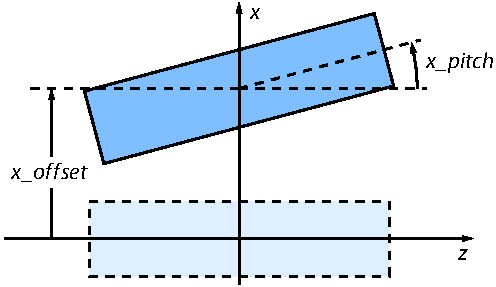
\includegraphics{pitch.eps}
  \caption{Geometry of Pitch and Offset attributes}
  \label{f:pitch}
\end{figure}

\begin{figure}[ht]
  \centering
  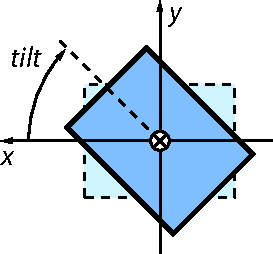
\includegraphics{tilt.eps}
  \caption{Geometry of a Tilt}
  \label{f:tilt}
\end{figure}

The tilt attribute rotates the element in the $(x, y)$ plane as shown
in figure~\ref{f:tilt}. The rotation axis is the $z$-axis at the
entrance face. The reference orbit is also rotated for any element
who's exit coordinates are not collinear with the entrance
coordinates. For example, a \vn{bend} or \vn{mirror} with a tilt of $\pi/2$ will bend a
beam vertically upward. The \vn{hkick} and \vn{vkick} attributes are
not affected by \vn{tilt} except for \vn{Kicker} and \vn{ElSeparator}
elements. Like MAD, \bmad allows the use of the \vn{tilt} attribute
without a value to designate a skew element. For example
\begin{example}
  q1: quad, l = 0.6, x_offset = 0.03, y_pitch = 0.001, tilt
\end{example}
Default tilts can be used for \vn{rbend}, \vn{sbend}, \vn{sol_quad},
\vn{quadrupole}, \vn{sextupole}, and \vn{octupole} elements.
The default tilt is $\pi/(2(n+1))$ where $n$ is the order of the 
element (n = 0 for bends, n = 1 for quadrupoles etc.) 

For all elements, offsets, pitches, and tilts are with
respect to the entrance coordinates (the local coordinates just before
the element.

The \vn{roll} attribute is only used for bends and rotates the bend,
along an axis that runs through the entrance point and exit point as
shown in figure~\ref{f:roll}. A \vn{roll} does not affect the
reference orbit. The major effect of a \vn{roll} is to give a vertical
kick to the beam. A positive \vn{roll} is similar to a positive
\vn{tilt}. That is, with a bend with positive bend angle, a positive
\vn{roll} will move the outside portion ($+x$ side) of the bend upward
and the inside portion (-$x$ side) downward. Much like car racetracks
which are typically slanted towards the inside of a turn.

\begin{figure}[ht]
  \centering
  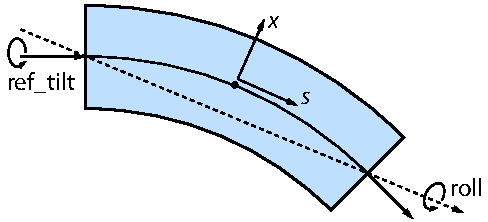
\includegraphics{roll.eps}
  \caption{Geometry of a Roll}
  \label{f:roll}
\end{figure}


%-----------------------------------------------------------------
\section{Hkick, Vkick, and Kick Attributes}
\label{s:kick}
\index{hkick|hyperbf}\index{bl_hkick|hyperbf}
\index{vkick|hyperbf}\index{bl_vkick|hyperbf}
\index{kick|hyperbf}\index{bl_kick|hyperbf}


\index{hkicker}
\index{vkicker}
\index{elseparator}
\index{kicker}
The kick attributes that an element may have are:
\begin{example}
  kick,  bl_kick  = <Real>  ! Used only with a Hkicker or Vkicker
  hkick, bl_hkick = <Real>
  vkick, bl_vkick = <Real>
\end{example}
\vn{kick}, \vn{hkick}, and \vn{vkick} attributes are the integrated
kick of an element in radians. \vn{kick} is only used for \vn{Hkicker}
and \vn{Vkicker} elements. All other elements that can kick use
\vn{hkick} and \vn{vkick}. The \vn{tilt} attribute will only rotate a
kick for \vn{Hkicker}, \vn{Vkicker}, \vn{Elseparator} and \vn{Kicker}
elements. This rule was implemented so that, for example, the
\vn{hkick} attribute for a skew quadrupole would represent a
horizontal steering. The \vn{bl_kick}, \vn{bl_hkick}, and
\vn{bl_vkick} attributes are the integrated field kick in
\vn{meters-Tesla}. Normally these are dependent attributes except if
they appear in the lattice file (\sref{s:depend}).

%-----------------------------------------------------------------
\section{Aperture and Limit Attributes}
\label{s:limit}
\index{aperture|hyperbf}
\index{limit|hyperbf}
\index{aperture_at|hyperbf}

\begin{figure}[ht]
  \centering
  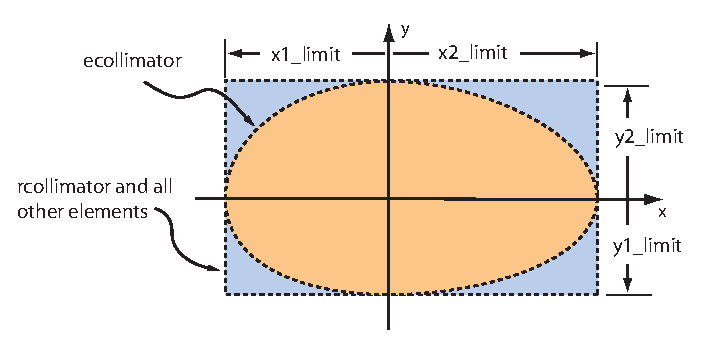
\includegraphics{apertures.eps}
  \caption{Apertures for ecollimator and rcollimator elements}
  \label{f:limit}
\end{figure}

\index{ecollimator}
\index{rcollimator}
\index{x_limit|hyperbf}
\index{y_limit|hyperbf}
\index{x1_limit|hyperbf}
\index{y1_limit|hyperbf}
\index{x2_limit|hyperbf}
\index{y2_limit|hyperbf}
\index{x_offset|hyperbf}
\index{offset_moves_aperture|hyperbf}
\index{aperture_at}
\index{aperture_type}
The aperture attributes are:
\begin{example}
  x1_limit      = <Real>      ! Horizontal, negative side, aperture limit
  x2_limit      = <Real>      ! Horizontal, positive side, aperture limit
  y1_limit      = <Real>      ! Vertical, negative side, aperture limit
  y2_limit      = <Real>      ! Vertical, positive side, aperture limit
  x_limit       = <Real>      ! Alternative to specifying x1_limit and x2_limit
  y_limit       = <Real>      ! Alternative to specifying y1_limit and y2_limit
  aperture      = <Real>      ! Alternative to specifying x_limit and y_limit
  aperture_at   = <Switch>    ! What end aperture is at.
  aperture_type = <Switch>    ! What type of aperture it is.
  offset_moves_aperture = <Logical> ! Element offsets affect aperture position
\end{example}
\vn{x1_limit}, \vn{x2_limit}, \vn{y1_limit}, and \vn{y2_limit} specify
the half--width of the aperture of an element as shown in
figure~\ref{f:limit}. A zero \vn{x1_limit}, \vn{x2_limit},
\vn{y1_limit}, or \vn{y2_limit} is interpreted as no aperture in the
appropriate plane.

By default, apertures are assumed to be
rectangular except that an \vn{Ecollimator} has a elliptical aperture.
This can be changed by setting the \vn{aperture_type} attribute. The possible 
values of this attribute are:
\begin{example}
  rectanular
  elliptical
\end{example}

To avoid numerical overflow and other errors in tracking, a particle
will be considered to have hit an aperture in an element, even if
there are no apertures set for that element, if its orbit exceeds 1000
meters. Additionally, there are other situations where a particle will
be considered lost. For example, if a particle's trajectory does
not intersect the output face in a bend.

For convenience, \vn{x_limit} can be used to set \vn{x1_limit} and
\vn{x2_limit} to a common value. Similarly, \vn{y_limit} can be used
to set \vn{y1_limit} and \vn{y2_limit}.  The \vn{aperture} attribute
can be use to set all four \vn{x1_limit}, \vn{x2_limit}, \vn{y1_limit}
and \vn{y2_limit} to a common value. Internally, the \bmad code does {\em not}
store \vn{x_limit}, \vn{y_limit}, or \vn{aperture}. This means that
using \vn{x_limit}, \vn{y_limit} or aperture in arithmetic expressions is
an error:
\begin{example}
  q2: quad, aperture = q1[aperture]   ! THIS IS AN ERROR!
  q2: quad, aperture = q1[x1_limit]   ! Correct
\end{example}

\index{tilt}
\index{x_offset}
\index{y_offset}
\index{x_pitch}
\index{y_pitch}
Normally, whether a particle hits an aperture or not is evaluated
independent of any element offsets (\sref{s:offset}). This is
equivalent to the situation where a beam pipe containing an aperture
is independent of the element the beam pipe passes through. This can
be changed by setting the \vn{offset_moves_aperture} attribute to
\vn{True}. In this case any offsets or pitches will be considered to
have shifted the aperture boundary. The exception here is that the
default for \vn{rcollimator} and \vn{ecollimator} elements is for
\vn{offset_moves_aperture} to be \vn{True}.

Even with \vn{offset_moves_aperture} set to \vn{True}, \vn{tilt}s will
not affect the aperture calculation. This is done, for example, so
that the tilt of a skew quadrupole does not affect the aperture. The
exception here is that tilting an \vn{rcollimator} or \vn{ecollimator}
element will tilt the aperture.

\index{entrance_end|hyperbf}
\index{exit_end|hyperbf}
\index{aperture_at}
By default the aperture is evaluated at the exit face only of the
element. This can be changed by setting the \vn{aperture_at} attribute.
Possible settings for \vn{aperture_at} are:
\begin{example}
  entrance_end
  exit_end  ! default
  both_ends
\end{example}
Note that the entrance and exit ends of an element are independent of
which direction particles are tracked through an element. Thus if a
particle is tracked backwards it enters an element at the ``exit end''
and exits at the ``entrance end''.

Examples:
\begin{example}
  q2: quad, aperture_type = elliptical  
  q1: quad, l = 0.6, x1_limit = 0.045, offset_moves_aperture = T
  q1[y1_limit] = 0.03
  q1[y2_limit] = 0.03
  q1[y_limit] = 0.03  ! equivalent to the proceeding 2 lines.  
  q1[aperture_at] = both_ends
\end{example}

%-----------------------------------------------------------------
\section{Length Attributes}
\label{s:l}

\index{l|hyperbf}
\index{l_chord|hyperbf}
\index{rbend}
\index{sbend}
The length attributes are
\begin{example}
  l       = <Real>  ! 
  l_chord           ! Chord length of a bend. Dependent attribute.
\end{example}
The length \vn{l} is the path length of the reference
particle. The one exception that that for an \vn{Rbend} the length
\vn{l} is the chord length (\sref{s:bend}). Internally, \bmad converts
all \vn{Rbend}s to \vn{Sbend}s and stores the chord length
under the \vn{l_chord} attribute.

\index{wiggler}
Note that for \vn{Wiggler}s
the length \vn{l} is not the same as the path length for a particle
with the reference energy starting on the reference orbit.

%-----------------------------------------------------------------
\section{Is_on Attribute}
\label{s:is.on}
\index{is_on|hyperbf}

The \vn{is_on} attribute
\begin{example}
  is_on = <Logical>
\end{example}
is used to turn an element off. Turning
an element off essentially converts it into a drift.
Example
\begin{example}
  q1: quad, l = 0.6, k1 = 0.95
  q1[is_on] = False
\end{example}

\vn{is_on} does not affect any apertures that are set. Additionally,
\vn{is_on} does not affect the reference orbit. Therefore, turning 
off an \vn{lcavity} will not affect the reference energy.

%-----------------------------------------------------------------
\section{Multipole Attributes: An, Bn, KnL, Tn}
\label{s:multip}

\index{multipole!an, bn|hyperbf} 
\index{multipole!knl, tn|hyperbf} 
\index{ab_multipole}
\index{multipole}
\index{radius}
A \vn{Multipole} element specifies its multipole components using an
Amplitude (\vn{KnL}) and a tilt (\vn{Tn})
\begin{example}
  KnL = <Real>
  Tn  = <Real>  ! Default is $pi$/(2n + 2)
\end{example}
\vn{AB_Multipole} and all other elements that
have multipole attributes specify the multipoles using normal
(\vn{Bn}) and skew (\vn{An}) components 
\begin{example}
  An = <Real>
  Bn = <Real>
\end{example}
Here \vn{n} ranges from 0
(dipole component) through 20. Example:
\begin{example}
  q1: quadrupole, b0 = 0.12, a20 = 1e7, radius = 0.045
\end{example}

Multipole formulas for are given in \sref{s:fields}.  Note that for
\vn{Multipole} and \vn{AB_multipole} (but not any other element) a
non-zero dipole component will affect the reference orbit (just like a
normal dipole will).

The \vn{Tn} tilt component without a value takes a default of $pi$/(2n + 2) which makes
the component \vn{skew}.
Example:
\begin{example}
  m: multipole, k1l = 0.45, t1  ! Skew quadrupole
\end{example}

For everything other than a \vn{Multipole} and \vn{AB_multipole}, the
multipole strength is scaled by a factor $F \, r_0^{n_\text{ref}} /
r_0^n$ (cf.~\Eq{ababf}) where $F$ is the strength of the element (for
example $F$ is $K1 \cdot L$ for a quadrupole), and $r_0$ is the
``measurement radius'' and is set by the \vn{radius} attribute. The
default value of $r_0$, if the \vn{radius} is not given, is 1.0.

%-----------------------------------------------------------------
\section{Instrumental Measurement Attributes}
\label{s:meas.attrib}

\index{instrument}\index{monitor}\index{marker}
\index{x_gain_err}\index{y_gain_err}\index{Crunch}\index{noise}
\index{x_gain_calib}\index{y_gain_calib}\index{crunch_calib}
\index{x_offset}\index{y_offset}\index{tilt}
\index{x_offset_calib}\index{y_offset_calib}\index{tilt_calib}
\index{de_eta_meas}\index{n_sample}\index{osc_amplitude}

\vn{Instrument}, \vn{Monitor}, and \vn{Marker} elements have special
attributes to describe orbit, betatron phase, dispersion and coupling
measurements. These attributes are:
\hfill\break
\hspace*{0.1in}
\begin{tabular}{llll}
  {\em Attribute}     &            &! {\em Symbol} (\sref{s:meas.calc}) & \\
  \vn{tilt}           &= <Real>    &! $\theta_t$            & See \sref{s:offset} \\ 
  \vn{x_offset}       &= <Real>    &! $x_{\mss{err}}$       & See \sref{s:offset} \\ 
  \vn{y_offset}       &= <Real>    &! $y_{\mss{err}}$       & See \sref{s:offset} \\ 
  \vn{x_gain_err}     &= <Real>    &! $dg_{x,\mss{err}}$    & Horizontal gain error \\ 
  \vn{y_gain_err}     &= <Real>    &! $dg_{y,\mss{err}}$    & Vertical gain error \\ 
  \vn{crunch}         &= <Real>    &! $\psi_{\mss{err}}$    & Crunch angle \\ 
  \vn{tilt_calib}     &= <Real>    &! $\theta_{\mss{err}}$  & tilt angle calibration \\ 
  \vn{x_offset_calib} &= <Real>    &! $x_{\mss{cal}}$       & Horizontal offset calibration \\ 
  \vn{y_offset_calib} &= <Real>    &! $y_{\mss{cal}}$       & Vertical offset calibration \\ 
  \vn{x_gain_calib}   &= <Real>    &! $dg_{x,\mss{cal}}$    & Horizontal gain calibration \\ 
  \vn{y_gain_calib}   &= <Real>    &! $dg_{y,\mss{cal}}$    & Vertical gain calibration \\ 
  \vn{crunch_calib}   &= <Real>    &! $\psi_{\mss{cal}}$    & Crunch angle calibration \\ 
  \vn{noise}          &= <Real>    &! $n_f$                 & Noise factor \\ 
  \vn{de_eta_meas}    &= <Real>    &! $dE/E$                & Percent change in energy \\ 
  \vn{n_sample}       &= <Real>    &! $N_s$                 & Number of sampling points \\ 
  \vn{osc_amplitude}  &= <Real>    &! $A_{\mss{osc}}$       & Oscillation amplitude \\ 
\end{tabular}
\hfill\break
A program can use these quantities to calculate ``measured'' values from the
``laboratory'' values. Here, ``laboratory'' means as calculated from some model lattice.
See \sref{s:meas.calc} for the conversion formulas.

\chapter{Tracking and Transfer Matrix Calculation Methods}

Typically, there are several ways to do tracking and transfer matrix
calculations for a given element type within \bmad. What method is
used is selected on an element--by--element basis using an element's
\vn{tracking_method} and \vn{mat6_calc_method} attributes (mat6 refers
to the size of the 6 by 6 transfer matrices). By supplying the
appropriate routines a programmer can extend \bmad\ to do customized
tracking. In general \bmad assumes that particles are
ultra--relativistic. The methods that do not make this assumption are:
\vn{Boris}, \vn{Adaptive_Boris}, \vn{Symp_Lie_Ptc}, \vn{Symp_map}, and \vn{Taylor}

If this is not the case 

%----------------------------------------------------------------------------
\section{tracking\_method Switches}
\label{s:tkm}
\index{Tracking method|textbf}

Below are listed the methods for the \vn{tracking_method}
attribute with an explanation of what the different methods do. A
table giving which methods are available with which element types is give
in Table~\ref{t:track_methods}. 

A note on terminology: Adaptive step size control used with the
\vn{Adaptive_Boris} and \vn{Runge_Kutta} integrators means that 
instead of taking fixed step sizes the integrator chooses the proper
step size so that the error in the tracking is below the maximum
allowable error set by \vn{rel_tol} and \vn{abs_tol} tolerances. The
advantage of step size control is that the integrator uses a smaller
step size when needed (the fields are rapidly varying), but makes
larger steps when it can. The disadvantage is that a step is more
computationally intensive since the error in a step is estimated by
repeating a step using two mini steps. If the fields are rather
uniform and you know what a good step size is you can save time by using
a fixed step size.

\begin{description}
\item[\vn{Adaptive\_Boris}]
Second order Boris integration\cite{b:boris} with adaptive step size control.
This should be nearly symplectic but slow.

\item[\vn{Boris}]
Second order Boris Integration\cite{b:boris}. Like \vn{Runge_Kutta},
\vn{Boris} does tracking by integrating the equation of
motion. \vn{Boris} handles both electric and magnetic fields and does
not assume that the particle is ultra--relativistic. \vn{Boris} preserves
conserved quantities more accurately than \vn{Runge_Kutta}.

\item[\vn{Bmad\_Standard}]
Uses formulas for tracking. The emphasis here is on speed and not
symplecticity. Appropriate when you are interested in single turn
stuff. May be appropriate for long term tracking depending upon how
many turns are tracked and what kind of elements are involved. 

\item[\vn{Custom}]
This method will call a routine \vn{track1_custom} which must be
supplied by the programmer implementing the custom tracking. The
default \vn{track1_custom} supplied with the \bmad\ release will print
an error message and stop the program if it is called which probably
indicates a program linking problem.

\item[\vn{Linear}]
Linear just uses the 0th order vector with the 1st order 6x6 transfer
matrix for an element. Very simple.  Depending upon how the transfer
matrix was generated this may or may not be symplectic.

\item[\vn{MAD}]
This uses the MAD 2nd order transfer map.

\item[\vn{Runge\_Kutta}]
This uses a 4\Th\ order Runge Kutta integration algorithm with adaptive
step size control.  This is essentially the \vn{ODEINT} subroutine
from Numerical Recipes\cite{b:nr}. This may be slow but it should be
accurate. This method is non-symplectic.

\item[\vn{Symp\_Lie\_Bmad}]
Symplectic tracking using a Hamiltonian with Lie operation techniques.
This is similar to \vn{Symp_Lie_PTC} (see below) except this uses a
\bmad\ routine. By bypassing some of the generality inherent in PTC's routines
\vn{Symp_Lie_Bmad} achieves about a factor of 10 improvement in speed over
\vn{Symp_Lie_PTC}. However, \vn{Symp_lie_Bmad} is
currently only implemented for Wigglers.

\item[\vn{Symp\_Lie\_PTC}]
Symplectic tracking using a Hamiltonian with Lie operator techniques.
This uses Etienne's PTC software for the calculation. This method is
symplectic but can be slow.

\item[\vn{Symp\_Map}]
This uses a partially inverted, implicit Taylor map. The calculation
uses Etienne's PTC software.  Since the map is implicit, a Newton
search method must be used. This will slow things down from the Taylor
method but this is guaranteed symplectic.

\item[\vn{Taylor}]
This uses a Taylor map generated from Etienne's PTC
package. Generating the map may take time but once you have it it
should be very fast. One possible problem with using a Taylor map is
that you have to worry about the accuracy if you do tracking at points
that are far from the expansion point about which the map was
made. This method is non-symplectic away from the expansion point. 

\item[\vn{Wiedemann}]
This is Wiedemann's hard edge model of a wiggler
\cite{wiedemann}. This model divides a wiggler pole into a constant 
bend rectangular section with drifts at either end. The total length
of the model pole matches the actual pole length of the element. The
strength of the bend and the lengths of the bend and drifts are
adjusted so that the vertical focusing and horizontal deflection are
the same in the modal as with a model assuming a sinusoidally varying
field. \bmad\ augments this model by assuming that the horizontal
deflection varies as the $\sinh$ with vertical offset.  Since
Wiedemann's model does not include longitudinal fields it is not clear
that it can be used for long term tracking.

\end{description}

\vfill \break
{\vfill}

\begin{table}[h]
\centering {
\begin{tabular}{|l|c|c|c|c|c|c|c|c|c|c|c|c|} \hline
\rule{0pt}{80pt} &
\begin{sideways}\vn{Adaptive_Boris}\end{sideways} &
\begin{sideways}\vn{Bmad_Standard}\end{sideways} &
\begin{sideways}\vn{Boris}\end{sideways} &
\begin{sideways}\vn{Custom}\end{sideways} &
\begin{sideways}\vn{Linear}\end{sideways} &
\begin{sideways}\vn{MAD}\end{sideways} &
\begin{sideways}\vn{Runge_Kutta}\end{sideways} &
\begin{sideways}\vn{Symp_Lie_Bmad}\end{sideways} &
\begin{sideways}\vn{Symp_Lie_PTC}\end{sideways} &
\begin{sideways}\vn{Symp_Map}\end{sideways} &
\begin{sideways}\vn{Taylor}\end{sideways} &
\begin{sideways}\vn{Wiedemann}\end{sideways}
\\ \hline
%                               AB  BS   B   C   L   M  RK  SLB SLP SM   T   W
  \vn{ab_multipole}            &   & D &   & X & X &   &   &   & X & X & X &   \\ \hline 
  \vn{beambeam}                &   & D &   & X & X &   &   &   &   &   &   &   \\ \hline 
  \vn{bend_sol_quad}           &   &   &   &   &   &   &   & D &   &   &   &   \\ \hline 
  \vn{custom}                  & X &   & X & D & X &   & X &   &   &   &   &   \\ \hline 
  \vn{drift}                   & X & D & X & X & X & X & X &   & X & X & X &   \\ \hline 
  \vn{ecollimator}             & X & D & X & X & X &   & X &   & X & X & X &   \\ \hline 
  \vn{elseparator}             & X & D & X & X & X & X & X &   & X & X & X &   \\ \hline 
  \vn{hkicker}                 & X & D & X & X & X &   & X &   & X & X & X &   \\ \hline 
  \vn{instrument}              & X & D & X & X & X &   & X &   & X & X & X &   \\ \hline 
  \vn{kicker}                  & X & D & X & X & X &   & X &   & X & X & X &   \\ \hline 
  \vn{lcavity}                 &   & D &   & X & X &   &   &   &   &   &   &   \\ \hline 
  \vn{marker}                  &   & D &   & X & X &   &   &   & X & X & X &   \\ \hline 
  \vn{monitor}                 & X & D & X & X & X &   & X &   & X & X & X &   \\ \hline 
  \vn{multipole}               &   & D &   & X & X &   &   &   & X & X & X &   \\ \hline 
  \vn{octupole}                & X & D & X & X & X &   & X &   & X & X & X &   \\ \hline
  \vn{patch}                   &   & D &   & X &   &   &   &   &   &   &   &   \\ \hline
  \vn{quadrupole}              & X & D & X & X & X & X & X &   & X & X & X &   \\ \hline
  \vn{rbend}                   &   & D &   & X & X & X &   &   & X & X & X &   \\ \hline
  \vn{rcollimator}             & X & D & X & X & X &   & X &   & X & X & X &   \\ \hline
  \vn{rfcavity}                &   & D &   & X & X & X &   &   & X & X & X &   \\ \hline
  \vn{sbend}                   &   & D &   & X & X & X &   &   & X & X & X &   \\ \hline
  \vn{sextupole}               & X & D & X & X & X & X & X &   & X & X & X &   \\ \hline
  \vn{solenoid}                & X & D & X & X & X & X & X &   & X & X & X &   \\ \hline
  \vn{sol_quad}                & X & D & X & X & X & X & X &   & X & X & X &   \\ \hline
  \vn{taylor}                  &   & D &   & X & X &   &   &   &   &   &   &   \\ \hline
  \vn{vkicker}                 & X & D & X & X & X &   & X &   & X & X & X &   \\ \hline
  \vn{wiggler} (periodic type) &   & D &   & X & X &   &   &   &   &   &   & X \\ \hline
  \vn{wiggler} (map type)      & X & D & X & X & X &   & X & X & X & X & X &   \\ \hline
\end{tabular}
}
\caption[Table of available {\bf tracking\_method}\ switches for a
given element type.]{Table of available {\bf tracking\_method}\
switches for a given element type. D denotes the default method. X
denotes an available method.}
\label{t:track_methods}
\end{table}

\vfill\break

%----------------------------------------------------------------------------
\section{mat6\_calc\_method Switches}
\label{s:xfer}
\index{Mat6_calc_method|textbf}

Below are listed the methods for the \vn{mat6_calc_method}
attribute with an explanation of what the different methods do. A
table giving which methods are available with which element types is give
in Table~\ref{t:mat6_methods}. 

For methods that do not necessarily produce a symplectic matrix the
\vn{symplectify} attribute of an element can be set to \vn{True} to
solve the problem. See section~\ref{s:symp_method}. 

Symplectic integration is like ordinary integration of a function f(x)
but what is integrated here is a Taylor map. Truncating the map to
0\Th\ order gives the particle trajectory and truncating to 1\St\
order gives the transfer matrix (Jacobian).  The order at which a
Taylor series is truncated at is set by \vn{taylor_order} (see
Section~\ref{s:param}. Like ordinary integration there are various
formulas that one can use to do symplectic integration. In \bmad\ (or
more precisely Etienne's PTC) you can use one of 3 methods. This is
set by \vn{integration_ord}.  \vn{integration_ord} = n where $n$ is
allowed by PTC to be 2, 4, or 6. With an integration order of $n$ the
error in an integration step scales as $dz^n$ where $dz$ is step
size. The step size $dz$ is set by the length of the element and the
value of \vn{num_steps}. Remember, as in ordinary integration, higher
integration order does not necessarily imply higher accuracy.

\begin{description}

\index{Mat6_calc_method!Bmad_Standard}
\item[\vn{Bmad\_Standard}]
Uses formulas for the calculation. The emphasis here is on speed and not
symplecticity. Appropriate when you are interested in single turn
stuff. May be appropriate for long term tracking depending upon how
many turns are tracked and what kind of elements are involved. 

\index{Mat6_calc_method!Custom}
\item[\vn{Custom}]
This method will call a routine \vn{make_mat6_custom} which must be
supplied by the programmer implementing the custom transfer matrix
calculation. The default \vn{make_mat6_custom} supplied with the
\bmad\ release will print an error message and stop the program if it
is called which probably indicates a program linking problem.

\index{Mat6_calc_method!MAD}
\item[\vn{MAD}]
This uses the MAD 2nd transfer map.

\index{Mat6_calc_method!Symp_lie_Bmad}
\item[\vn{Symp\_Lie\_Bmad}]
A Symplectic calculation using a Hamiltonian with Lie operator techniques.
This is similar to \vn{Symp_Lie_PTC} (see below) except this uses a
\bmad\ routine. By bypassing some of the generality inherent in PTC's routines
\vn{Symp_Lie_Bmad} achieves about a factor of 10 improvement in speed over
\vn{Symp_Lie_PTC}. However, \vn{Symp_lie_Bmad} is
currently only implemented for Wigglers.

\index{Mat6_calc_method!Symp_Lie_PTC}
\item[\vn{Symp\_Lie\_PTC}]
Symplectic integration using a Hamiltonian and Lie operators.
This uses Etienne's PTC software for the calculation.
This method is symplectic but can be slow.

\index{Mat6_calc_method!Taylor}
\item[\vn{Taylor}]
This uses a Taylor map generated from Etienne's PTC
package. Generating the map may take time but once you have it it
should be very fast. One possible problem with using a Taylor map is
that you have to worry about the accuracy if you do a calculation at points
that are far from the expansion point about which the map was
made. This method is non-symplectic away from the expansion point. 

\index{Mat6_calc_method!Tracking}
\item[\vn{Tracking}]
This uses the tracking method set by \vn{tracking_method} to track 6
particles around the central orbit. This method is susceptible to inaccuracies
caused by nonlinearities. Furthermore this method
is almost surely slow. While non--symplectic, the advantage of this method
is that it is directly related to any tracking results.

\end{description}

\vfill \break
\vfill

\begin{table}[th]
\centering {
\begin{tabular}{|l|c|c|c|c|c|c|c|} \hline
\rule{0pt}{80pt} &
\begin{sideways}\vn{Bmad_Standard}\end{sideways} &
\begin{sideways}\vn{Custom}\end{sideways} &
\begin{sideways}\vn{MAD}\end{sideways} &
\begin{sideways}\vn{Symp_Lie_Bmad}\end{sideways} &
\begin{sideways}\vn{Symp_Lie_PTC}\end{sideways} &
\begin{sideways}\vn{Taylor}\end{sideways} &
\begin{sideways}\vn{Tracking}\end{sideways}
\\ \hline
%                               BS   C   M  SLB SLP Tlr Trk 
  \vn{ab_multipole}            & D & X &   &   & X & X &   \\ \hline 
  \vn{beambeam}                & D & X &   &   &   &   & X \\ \hline 
  \vn{bend_sol_quad}           &   &   &   & D &   &   & X \\ \hline 
  \vn{custom}                  &   & D &   &   &   &   & X \\ \hline 
  \vn{drift}                   & D & X & X &   & X & X & X \\ \hline 
  \vn{ecollimator}             & D & X &   &   & X & X & X \\ \hline 
  \vn{elseparator}             & D & X & X &   & X & X & X \\ \hline 
  \vn{hkicker}                 & D & X &   &   & X & X & X \\ \hline 
  \vn{instrument}              & D & X &   &   & X & X & X \\ \hline 
  \vn{kicker}                  & D & X &   &   & X & X & X \\ \hline 
  \vn{lcavity}                 & D & X &   &   &   &   & X \\ \hline 
  \vn{marker}                  & D & X &   &   & X & X & X \\ \hline 
  \vn{monitor}                 & D & X &   &   & X & X & X \\ \hline 
  \vn{multipole}               & D & X &   &   & X & X &   \\ \hline 
  \vn{octupole}                & D & X &   &   & X & X & X \\ \hline
  \vn{patch}                   & D & X &   &   &   &   &   \\ \hline
  \vn{quadrupole}              & D & X & X &   & X & X & X \\ \hline
  \vn{rbend}                   & D & X & X &   & X & X & X \\ \hline
  \vn{rcollimator}             & D & X &   &   & X & X & X \\ \hline
  \vn{rfcavity}                & D & X & X &   & X & X & X \\ \hline
  \vn{sbend}                   & D & X & X &   & X & X & X \\ \hline
  \vn{sextupole}               & D & X & X &   & X & X & X \\ \hline
  \vn{solenoid}                & D & X & X &   & X & X & X \\ \hline
  \vn{sol_quad}                & D & X & X &   & X & X & X \\ \hline
  \vn{taylor}                  & D & X &   &   &   &   &   \\ \hline
  \vn{vkicker}                 & D & X &   &   & X & X & X \\ \hline
  \vn{wiggler} (periodic type) & D & X &   &   &   &   & X \\ \hline
  \vn{wiggler} (map type)      & D & X &   & X & X & X & X \\ \hline
\end{tabular}
}

\caption[Table of available \vn{mat6\_calc\_method}\ switches for a
given element type.]{Table of available \vn{mat6\_calc\_method}\
switches for a given element type. D denotes the default method.  X
denotes an available method.}

\label{t:mat6_methods}
\end{table}

\vfill \break

chapter{Beam Lines, Replacement Lists, and Branching}
\label{c:sequence}

\index{MAD}
To \bmad a ``lattice''\index{lattice} is the sequence of physical
elements that is to be studied. The lattice is constructed in the
input lattice file using what are know as Beam Lines and Replacement
Lists. Beam Lines are further subdivided into Lines with and without
replacement arguments. This essentially corresponds to the \mad
definition of Lines and Lists. There can be multiple Beam Lines and
Replacement Lists defined in a lattice file and Lines and Lists can be
nested inside other Lines and Lists. The particular Line that defines
the lattice to be analyzed by \bmad is selected by the \vn{use}
statement. For example
\begin{example}
  use, my_line
\end{example}
would pick the Line \vn{my_line} for analysis. 
Note that the names of the elements in the
lattice are always converted to upper case.

\bmad associates a number with each element staring at 1 for the first
element in the lattice, 2 for the second element, etc. Additionally,
\bmad always automatically creates a 0\Th element to mark the
beginning of the lattice. The name of this element is always \vn{BEGINNING}.

%-----------------------------------------------------------------------------
\section{Beam Lines without Arguments}
\label{s:lines.wo.arg}
\index{line|hyperbf}

A Beam Line without arguments has the format
\begin{example}
  label: line = (member1, member2, ...)
\end{example}
where \vn{member1}, \vn{member2}, etc. are either elements, other Beam
Lines or Replacement Lists, or sublines enclosed in parentheses.
Example:
\begin{example}
  line1: line = (a, b, c)
  line2: line = (d, line1, e)
  use, line2
\end{example}
This example shows how an Line member can refer to another Beam Line.
This is helpful if the same sequence of elements appears repeatedly in
the lattice. When \vn{line2} is expanded to form the lattice the
definition of \vn{line1} will be inserted in to produce the following
lattice for analysis
\begin{example}
  (d, a, b, c, e)
\end{example}
Note: In the expanded lattice, any \vn{Null_Ele} type elements
(\sref{s:null.ele}) will be discarded. For example, if element \vn{b}
in the above example is a \vn{Null_Ele} then the actual expanded
lattice will be:
\begin{example}
  (d, a, c, e)
\end{example}

A member that is a Line or List can be reflected 
(elements taken in reverse order) if
a negative sign is put in front of it. For example:
\begin{example}
  line1: line = (a, b, c)
  line2: line = (d, -line1, e)
\end{example}
\vn{line2} when expanded gives
\begin{example}
  (d, c, b, a, e)
\end{example}
Reflecting a subline will also reflect any sublines of the subline. For
example:
\begin{example}
  line0: line = (y, z)
  line1: line = (line0, b, c)
  line2: line = (d, -line1, e)
\end{example}
\vn{line2} when expanded gives
\begin{example}
  (d, c, b, z, y, e)
\end{example}

A repetition count, which is an integer followed by an asterisk, 
means that the member is
repeated. For example
\begin{example}
  line1: line = (a, b, c)
  line2: line = (d, 2*line1, e)
\end{example}
\vn{line2} when expanded gives
\begin{example}
  (d, a, b, c, a, b, c, e)
\end{example}
Repetition count can be combined with reflection. For example
\begin{example}
  line1: line = (a, b, c)
  line2: line = (d, -2*line1, e)
\end{example}
\vn{line2} when expanded gives
\begin{example}
  (d, c, b, a, c, b, a, e)
\end{example}
Instead of the name of a line, subline members can also be given as an explicit 
list using parentheses. For example, the previous example could be rewritten as
\begin{example}
  line2: line = (d, -2*(a, b, c), e)
\end{example}

A line can have the \vn{multipass} attribute. This is covered in
\sref{s:multipass}.

%-----------------------------------------------------------------------------
\section{Beam Lines with Replaceable Arguments}
\index{line!with arguments}

Beam lines can have an argument list using the following syntax
\begin{example}
  line_name(dummy_arg1, dummy_arg2, ...): LINE = (member1, member2, ...)
\end{example}
The dummy arguments are replaced by the actual arguments when the Line is used
elsewhere. For example:
\begin{example}
  line1(DA1, DA2): line = (a, DA2, b, DA1)
  line2: line = (h, line1(y, z), g)
\end{example}
When \vn{line2} is expanded the actual arguments of \vn{line1}, in this
case \vn(y, z), replaces the dummy arguments \vn{(DA1, DA2)} to give for
\vn{line2}
\begin{example}
  h, a, z, b, y, g
\end{example} 
\index{MAD}
Unlike \mad, Beam Line actual arguments can only be elements or Beam Lines. 
Thus the following is not allowed
\begin{example}
  line2: line = (h, line1(2*y, z), g)   ! NO: 2*y NOT allowed as an argument.
\end{example}

%-----------------------------------------------------------------------------
\section{Replacement Lists}
\index{list}

When a lattice is expanded, all the lattice members that correspond to a 
name of a Replacement List 
are replaced successively, by the members
in the Replacement List. The general syntax is
\begin{example}
  label: LIST = (member1, member2, ...)
\end{example}
For example:
\begin{example}
  list1: list = (a, b, c)
  line1: line = (z1, list1, z2, list1, z3, list1, z4, list1)
  use, line1
\end{example}
When the lattice is expanded the first instance of \vn{list1} in
\vn{line1} is replaced by \vn{a} (which is the first element of
\vn{list1}), the second instance of \vn{list1} is replaced by \vn{b},
etc. If there are more instances of \vn{list1} in the lattice then
members of \vn{list1}, the replacement starts at the beginning of
\vn{list1} after the last member of \vn{list1} is used. In this case the
lattice would be:
\begin{example}
  z1, a, z2, b, z3, c, z4, a
\end{example}
\index{MAD}
Unlike \mad members of a replacement list can only be simple elements 
without reflection or repetition count and not other Lines or Lists. 
For example the following is not allowed:
\begin{example}
  list1: list = (2*a, b)  ! NO: No repetition count allowed.
\end{example}

%-----------------------------------------------------------------------------
\section{Line and List Tags}
\index{tags for Lines and Lists|hyperbf}
\label{s:tag}

When a lattice has repeating lines, it can be desirable to differentiate
between repeated elements. This can be done by tagging lines with a \vn{tag}. 
An example will make this clear:
\begin{example}
  line1: line = (a, b)
  line2: line = (line1, line1)
  use, line2
\end{example}
When expanded the lattice would be:
\begin{example}
  a, b, a, b
\end{example}
The first and third elements have the same name ``a'' and the second and fourth
elements have the same name ``b''. Using tags the lattice elements can be given
unique names. lines or lists are tagged  
using brackets \vn{[...]}. The general syntax is:
\begin{example}
  line_name[tag_name]                           ! Syntax for lines
  list_name[tag_name]                           ! Syntax for lists
  replacement_line[tag_name](arg1, arg2, ...)   ! Syntax for replacement lines.
\end{example}
Thus to differentiate the lattice elements in the above example \vn{line2} needs to
be modified using tags:
\begin{example}
  line1: line = (a, b)
  line2: line = (line1[t1], line1[t2])
  use, line2
\end{example}
In this case the lattice elements will have names of the form:
\begin{example}
  tag_name.element_name
\end{example}
In this particular example, the lattice with tagging will be:
\begin{example}
  t1.a, t1.b, t2.a, t2.b
\end{example}
Of course with this simple example one could have just as easily not used tags:
\begin{example}
  t1.a: a;   t2.a: a
  t1.b: b;   t2.b: b
  line1: line = (t1.a, t1.b, t2.a, t2.b)
  use, line2
\end{example}
But in more complicated situations tagging can make for compact lattice files.

When lines are nested, the name of an element is formed by concatenating the tags
together with dots in between in the form:
\begin{example}
  tag_name1.tag_name2. ... tag_name_n.element_name
\end{example}
An example will make this clear:
\begin{example}
  list1 = (g, h)
  line1(y, z) = (a, b)
  line2: line = (line1[t1](a, b))
  line3: line = (line2, list1[hh])
  line4: line = (line3[z1], line3[z2])
  use, line4
\end{example}
The lattice elements in this case are:
\begin{example}
  z1.t1.a, z1.t1.b, z1.hh.g, z2.t1.a, z2.t1.b, z1.hh.h 
\end{example}

\index{expand_lattice}
To modify a particular tagged element the lattice must be expanded
first (\sref{s:expand}). For example:
\begin{example}
  line1: line = (a, b)
  line2: line = (line1[t1], line1[t2])
  use, line2
  expand_lattice
  t1.b[k1] = 1.37
  b[k1] = 0.63       ! This statement does not have any effect
\end{example}
After the lattice has been expanded there is no connection between 
the original \vn{a} and \vn{b} elements and the elements in the lattice like
\vn{t1.b}. Thus the last line in the example where the \vn{k1} attribute of\vn{b} 
is modified do not have any effect on the lattice elements. 

%-----------------------------------------------------------------------------
\section{Branching}
\index{branch}\index{photon_branch}
\label{s:branching}

Lines that branch off from the main lattice can be defined in
\bmad. There are two types of branch elements. \vn{Branch} elements define
where the particle beam can branch off, say to a beam dump.
\vn{Photon_Branch} elements define the source point for photon beams.
Example:
\begin{example}
  erl: line = (..., b_mark, ...)             ! Define the main lattice with a branch 
  use, erl
  b_mark: branch, to = b_line, &             ! Define the branch point
               direction = -1, alias = dump  
  b_line: line = (..., q3d, ...)             ! Define the branch line
\end{example}

Branch lines can themselves have branch elements. A branch line always
starts out tangential to the line it is branching from. The
\vn{direction} attribute of the branch element indicates whether the
branch line is oriented in the forward or backward direction with
respect to the line being branched from. 

Branches are named after the setting of the \vn{alias} attribute of
the branch element. In the above example, the branch line would be
named \vn{DUMP}. If the \vn{alias} attribute is not set, the name of
the branch line (\vn{B_LINE} in the above example) is used instead.
To syntax for specifying a particular element in a branch line is
\begin{example}
  <branch_line_name>%<element_name>
\end{example}
Thus, in the above example, the syntax for specifying the \vn{Q3D}
element is \vn{DUMP%Q3D}. The main lattice specified by the \vn{use}
statement can be considered to be a branch and automatically has the
name \vn{MAIN}. Like the main lattice, \bmad always automatically
creates an element at the beginning of the branch called
\vn{BEGINNING}.

\chapter{Superposition}
\label{c:super}

\index{superposition}
This chapter covers the concept of \vn{superposition}.  \vn{Superposition} is used when elements
overlap spatially.  With \vn{superposition}, \vn{lord} and \vn{slave} elements (\sref{s:lord.slave})
are constructed by \bmad to hold the necessary information. The \vn{lord} elements will represent
the ``physical'' element while the \vn{slave} elements will embody the ``beam path''.

%-----------------------------------------------------------------------------
\section{Superposition Fundamentals}
\label{c:super.fund}

  \begin{figure}[tb]
  \centering 
  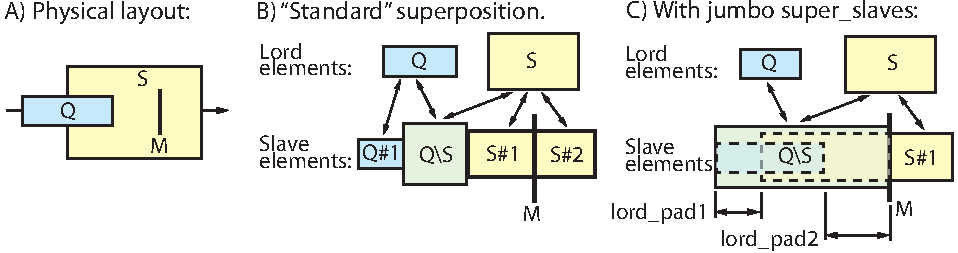
\includegraphics[width=0.95\textwidth]{superimpose-example.pdf} 
  \caption[Superposition example.]
{Superposition example. A) The physical layout involves a quadrupole partially inside a solenoid. B)
The standard superposition procedure involves creating \vn{super_slave} elements whose edges are at
the boundaries where the physical elements overlap. C) When jumbo \vn{super_slaves} are created, the
\vn{super_slaves} span the entire space where elements overlap.}
  \label{f:super.ex}
  \end{figure}

In practice the field at a particular point in the lattice may be due to more than one physical
element. One example of this is a quadrupole magnet inside a larger solenoid magnet as shown in
\fig{f:super.ex}A. \bmad has a mechanism to handle this using what is called ``superposition''. A
simple example shows how this works (also see section \sref{s:lord.slave}):
\begin{example}
  Q: quad, l = 4
  D: drift, l = 12
  S: solenoid, l = 8, superimpose, ref = Q, ele_origin = beginning
  M: marker, superimpose, ref = S, offset = 1
  lat: line = (Q, D)
  use, lat
\end{example}
The \vn{superimpose} attribute of element \vn{S} superimposes \vn{S} over the lattice \vn{(Q,
D)}. The placement of \vn{S} is such that the beginning of \vn{S} is coincident with the center of
\vn{Q} (this is is explained in more detail below). Additionally, a marker \vn{M} is superimposed at
a distance of +1~meter from the center of \vn{S}. The tracking part of the lattice
(\sref{s:lord.slave}) looks like:
\begin{example}
        Element   Key         Length  Total     
  1)    Q{\#}1       Quadrupole   2        2
  2)    Q{\B}S       Sol_quad     2        4
  3)    S{\#}1       Solenoid     3        7
  4)    M         Marker       0      
  4)    S{\#}2       Solenoid     3       10
  5)    D{\#}2       Drift        4       14
\end{example}
What \bmad has done is to split the original elements \vn{(Q, D)} at the edges of \vn{S} and then
\vn{S} was split where \vn{M} is inserted. The first element in the lattice, \vn{Q\#1}, is the part
of \vn{Q} that is outside of \vn{S}. Since this is only part of \vn{Q}, \bmad has put a \vn{\#1} in
the name so that there will be no confusion. (a single \vn{\#} has no special meaning other than the
fact that \bmad uses it for mangling names. This is opposed to a double \vn{\#\#} which is used to
denote the $N$\Th instance of an element (\sref{s:ele.match}). The next element, \vn{Q{\B}S}, is the
part of \vn{Q} that is inside \vn{S}. \vn{Q{\B}S} is a combination solenoid/quadrupole element as
one would expect. \vn{S{\#}1} is the part of \vn{S} that is outside \vn{Q} but before \vn{M}. This
element is just a solenoid. Next comes \vn{M}, \vn{S{\#}1}, and finally \vn{D\#2} is the rest of the
drift outside \vn{S}.

In the above example, \vn{Q} and \vn{S} will be \vn{super_lord} elements (\vn{s:lord.slave}) and
four elements in the tracking part of the lattice will be \vn{super_slave} elements. This is
illustrated in \fig{f:super.ex}B.

Notice that the name chosen for the \vn{sol_quad} element \vn{Q{\B}S} is dependent upon what is
being superimposed upon what. If \vn{Q} had been superimposed upon \vn{S} then the name would have
been \vn{S{\B}Q}.

When \bmad sets the element class for elements created from superpositions, \bmad will set the class
of the element to something other than an \vn{em_field} element (\sref{s:em.field}) if possible. If
no other possibilities exist, \bmad will use \vn{em_field}. For example, a \vn{quadrupole}
superimposed with a \vn{solenoid} will produce a \vn{sol_quad} \vn{super_slave} element but a
\vn{solenoid} superimposed with a \vn{rfcavity} element will produce an \vn{em_field} element since
there is no other class of element that can simultaneously handle solenoid and RF fields. An
\vn{em_field} \vn{super_slave} element will also be created if any of the superimposing elements 
have a non-zero orientation (\sref{s:offset}) since it is not, in general, possible to construct a slave
element that properly mimics the effect of a non-zero orientation.

  \begin{figure}[tb]
  \centering 
  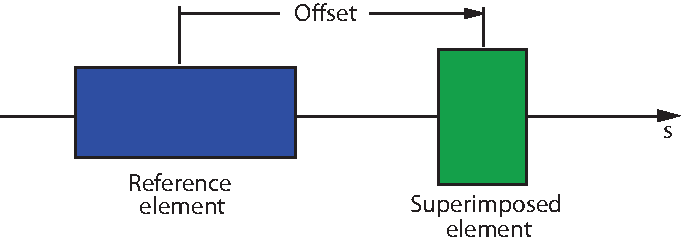
\includegraphics[width=0.8\textwidth]{superimpose.pdf} 
  \caption[Superposition Offset.]{
The superposition offset is the distance along the local reference orbit from the origin point of the
reference element to the origin point of the element being superimposed.
  }
  \label{f:superimpose}
  \end{figure}

With the lattice broken up like this \bmad has constructed something that can be easily
analyzed. However, the original elements \vn{Q} and \vn{S} still exist within the lord section of
the lattice. \bmad has bookkeeping routines so that if a change is made to the \vn{Q} or \vn{S}
elements then these changes can get propagated to the corresponding slaves. It does not matter which
element is superimposed. Thus, in the above example, \vn{S} could have been put in the Beam Line
(with a drift before it) and \vn{Q} could then have been superimposed on top and the result would
have been the same (except that the split elements could have different names).

If an element has zero length (for example, a \vn{marker} element), is superimposed, or is
superimposed upon, then the element will remain in the tracking part of the lattice and there will
be no corresponding lord element. See \fig{f:super.ex}.
 
Superimpose syntax:
\begin{example}
  Q: quad, superimpose, ...       ! Superimpose element Q.
  Q: quad, superimpose = T, ...   ! Same as above.
  Q: quad, ...                    ! First define element Q ...
  Q[superimpose] = T              !   ... and then superimpose.
  Q[superimpose] = F              ! Suppress superposition.
\end{example}
Superposition happens at the end of parsing so the last set of the \vn{superimpose} for an element
will override previous settings. 

It is also possible to superimpose an element using the \vn{superimpose} command which has the
syntax:
\begin{example}
  superimpose, element = <ele-name>, ...
\end{example}
With the same optional superposition parameters (\vn{ref}, \vn{offset}, etc.) given below.
Example:
\begin{example}
  superimpose, element = Q1, ref = B12, offset = 1.3, 
                               ele_origin = beginning, ref_origin = end
\end{example}
Note: Superposition using the superimpose statement allows superimposing the same element with
multiple reference elements and/or multiple offsets. The drawback is that superposition using the
superimpose statement may not be switched off later in the lattice file.

The placement of a superimposed element is illustrated in \fig{f:superimpose}. The placement of a
superimposed element is determined by three factors: An origin point on the superimposed element, an
origin point on the reference element, and an offset between the points. The attributes that
determine these three quantities are:
\index{ref}\index{offset}
\index{ref_origin}\index{ele_origin}
\begin{example}
  create_jumbo_slave = <Logical>     ! See \sref{s:jumbo.slave}
  wrap_superimpose   = <Logical>     ! Wrap if element extends past lattice ends?
  ref          = <lattice_element>
  offset       = <length>            ! default = 0
  ele_origin   = <origin_location>   ! Origin pt on element.
  ref_origin   = <origin_location>   ! Origin pt on ref element.
\end{example}
\vn{ref} sets the reference element. If \vn{ref} is not present then the start of the lattice is
used (more precisely, the start of branch 0 (\sref{s:branch.def})). Wild card characters
(\sref{s:ele.match} can be used with \vn{ref}. If \vn{ref} matches to multiple elements (which may
also happen without wild card characters if there are multiple elements with the name given by
\vn{ref}) in the lattice a superposition will be done, one for each match.

The location of the origin points are determined by the setting of \vn{ele_origin} and
\vn{ref_origin}.  The possible settings for these parameters are
\begin{example}
  beginning       ! Beginning (upstream) edge of element
  center          ! Center of element. Default.
  end             ! End (downstream) edge of element
\end{example}
\vn{center} is the default setting. \vn{Offset} is the longitudinal offset of the origin 
of the element being superimposed relative
to the origin of the reference element. The default offset is zero.  
A positive offset moves the element being superimposed in the \vn{downstream} direction if
the reference element has a normal longitudinal \vn{orientation} (\sref{s:ele.reverse}) and
vice versa for the reference element has a reversed longitudinal orientation.

Note: There is an old syntax, deprecated but still supported for now, where the origin points were
specified by the appearance of:
\begin{example}
  ele_beginning         ! Old syntax. Do not use.
  ele_center            ! Old syntax. Do not use.
  ele_end               ! Old syntax. Do not use.
  ref_beginning         ! Old syntax. Do not use.
  ref_center            ! Old syntax. Do not use.
  ref_end               ! Old syntax. Do not use.
\end{example}
For example, ``ele_origin = beginning'' in the old syntax would be ``ele_beginning''.

\index{drift}
\index{overlay}\index{group}\index{girder}
The element begin superimposed may be any type of element except \vn{drift}, \vn{group},
\vn{overlay}, and \vn{girder} control elements. The reference element used to position a
superimposed element may be a \vn{group} or \vn{overlay} element as long as the \vn{group} or
\vn{overlay} controls the attributes of exactly one element. In this case, the controlled element is
used as the reference element.

\index{geometry}\index{open}
By default, a superimposed element that extends beyond either end of the lattice will be wrapped
around so part of the element will be at the beginning of the lattice and part of the element will
be at the end. For consistency's sake, this is done even if the \vn{geometry} is set to \vn{open}
(for example, it is sometimes convenient to treat a circular lattice as linear). Example:
\begin{example}
  d: drift, l = 10
  q: quad, l = 4, superimpose, offset = 1
  machine: line = (d)
  use, machine
\end{example}
The lattice will have five elements in the tracking section:
\begin{example}
        Element    Key             Length
  0)    BEGINNING  Beginning_ele   0
  1)    Q{\#}2        Quadrupole      3   ! Slave representing beginning of Q element
  2)    D{\#}1        Drift           6
  3)    Q{\#}1        Quadrupole      1   ! Slave representing end of Q element
  4)    END        Marker          0
\end{example}
And the lord section of the lattice will have the element \vn{Q}. 

To not wrap an element that is being superimposed, set the \vn{wrap_superimpose} logical to \vn{False}.
Following the above example, if the definition of\vn{q} is extended by adding \vn{wrap_superimpose}:
\begin{example}
  q: quad, l = 4, superimpose, offset = 1, wrap_superimpose = F
\end{example}
In this instance there are four elements in the tracking section:
\begin{example}
        Element    Key             Length
  0)    BEGINNING  Beginning_ele   0
  1)    Q          Quadrupole      4    
  2)    D{\#}1        Drift           7
  4)    END        Marker          0
\end{example}
And the lord section of the lattice will not have any elements.

To superimpose a zero length element ``\vn{S}'' next to a zero length element ``\vn{Z}'', and to
make sure that \vn{S} will be on the correct side of \vn{Z}, set the \vn{ref_origin} appropriately.
For example:
\begin{example}
  S1: marker, superimpose, ref = Z, ref_origin = beginning
  S2: marker, superimpose, ref = Z, ref_origin = end
  Z: marker
\end{example}
The order of the elements in the lattice will be
\begin{example}
  S1, Z, S2
\end{example}
If \vn{ref_origin} is not present or set to \vn{center}, the ordering of the elements will be
arbitrary.

If a zero length element is being superimposed at a spot where there are other zero length elements,
the general rule is that the element will be placed as close as possible to the reference element.
For example:
\begin{example}
  S1: marker, superimpose, offset = 1
  S2: marker, superimpose, offset = 1
\end{example}
In this case, after \vn{S1} is superimposed at $s = 1$ meter, the superposition of \vn{S2} will
place it as close to the reference element, which in this case is the \vn{BEGINNING} elements at $s
= 0$, as possible. Thus the final order of the superimposed elements is:
\begin{example}
  S2, S1
\end{example}
To switch the order while still superimposing \vn{S2} second one possibility is to use:
\begin{example}
  S1: marker, superimpose, offset = 1
  S2: marker, superimpose, ref = S1, ref_origin = end
\end{example}

If a superposition uses a reference element, and there are $N$ elements in the lattice with the
reference element name, there will be $N$ superpositions. For example, the following will split in
two all the quadrupoles in a lattice:
\begin{example}
  M: null_ele, superimpose, ref = quadrupole::*
\end{example}
A \vn{null_ele} (\sref{s:null.ele}) element is used here so that there is no intervening element
between split quadrupole halves as there would be if a \vn{marker} element was used.


\index{drift!superposition}\index{pipe!superposition}
When a superposition is made that overlaps a drift, the drift, not being a "real" element,
vanishes. That is, it does not get put in the lord section of the lattice.  Note that if aperture
limits (\sref{s:limit}) have been assigned to a drift, the aperture limits can ``disappear'' when
the superposition is done. Explicitly, if the exit end of a drift has been assigned aperture limits,
the limits will disappear if the superimposed element overlays the exit end of the drift. A similar
situation applies to the entrance end of a drift. If this is not desired, use a \vn{pipe} element
instead. 

To simplify bookkeeping, a drift element may not be superimposed. Additionally, since drifts can
disappear during superposition, to avoid unexpected behavior the superposition reference element may
not be the $N$\Th instance of a drift with a given name. For example, if there are a number of drift
elements in the lattice named \vn{a_drft}, the following is not allowed:
\begin{example}
  my_oct: octupole, ..., superimpose, ref = a_drft##2  ! This is an error
\end{example}

When the attributes of a super_slave are computed from the attributes of its super_lords, some types
of attributes may be ``missing''. For example, it is, in general, not possible to set appropriate
aperture attributes (\sref{s:limit}) of a super_slave if the lords of the slave have differing
aperture settings. When doing calculations, \bmad will use the corresponding attributes stored in
the lord elements to correctly calculate things.

When superposition is done in a line where there is \vn{element reversal} (\sref{s:ele.reverse}),
the calculation of the placement of a superimposed element is also ``reversed'' to make the relative
placement of elements independent of any element reversal.  An example will make this clear:
\begin{example}
  d1: drift, l = 1
  d2: d1
  q1: quad, l = 0.1, superimpose, ref = d1, offset = 0.2, 
             ref_origin = beginning, ele_origin = beginning
  q2: q1, ref = d2
  p: patch, x_pitch = pi  ! Needed to separate reversed and unreversed.
  this_line: line = (d1, p, --d2)
  use, this_line
\end{example}
Since the reference element of the \vn{q2} superposition, that is \vn{d2}, is a reversed element,
\vn{q2} will be reversed and the sense of \vn{offset}, \vn{ref_origin}, and \vn{ele_origin} will be
reversed so that the position of \vn{q2} with respect to \vn{d2} will be the mirror image of the
position of \vn{q1} with respect to \vn{d1}. The tracking part of the lattice will be:
\begin{example}
  Element:           d1{\#}1    q1  d1{\#}2   d2{\#}2    q2   d2{\#}1
  Length:             0.2   0.1   0.7    0.7   0.1    0.3
  Reversed element?:   No    No    No    Yes   Yes    Yes
\end{example}

Superposition with \vn{line reflection} (\sref{s:lines.wo.arg}) works the same way as line reversal.

The \vn{no_superposition} statement (\sref{s:no.sup}) can be used to turn off superpositioning

%-----------------------------------------------------------------------------
\section{Superposition and Sub-Lines}
\label{c:super.sub.line}

Sometimes it is convenient to do simulations with only part of a lattice. The rule for how
superpositions are handled in this case is illustrated in the following example. Consider a lattice
file which defines a \vn{line} called \vn{full} which is defined by two sublines called \vn{sub1}
and \vn{sub2}:
\begin{example}
  sub1: line = {..., ele1, ...}
  sub2: line = {...}
  full: line = {sub1, sub2}
  m1: marker, superimpose, ref = ele1, offset = 3.7
  use, full
\end{example}
Now suppose you want to do a simulation using only the \vn{sub2} line. Rather than edit the original
file, one way to do this would be to create a second file which overrides the used line:
\begin{example}
  call, file = "full.bmad"
  use, sub2
\end{example}
where \vn{full.bmad} is the name of the original file. What happens to the superposition of \vn{m1}
in this case? Since \vn{m1} uses a reference element, \vn{ele1}, that is not in \vn{sub1}, \bmad
will ignore the superposition. Even though \bmad will ignore the superposition of \vn{m1} here,
\bmad will check that \vn{ele1} has been defined. If \vn{ele1} has not been defined, \bmad will
assume that there is a typographic error and issue an error message.

Notice that in this case it is important for the superposition to have an explicit reference element
since without an explicit reference element the superposition is referenced to the beginning of the
lattice. Thus, in the above example, if the superposition were written like:
\begin{example}
  m1: marker, superimpose, offset = 11.3
\end{example}
then when the \vn{full} line is used, the superposition of \vn{m1} is referenced to the beginning of
\vn{full} (which is the same as the beginning of \vn{sub1}) but when the \vn{sub2} line is used, the
superposition of \vn{m1} is referenced to the beginning of \vn{sub2} which is not the same as the
beginning of \vn{full}.

%-----------------------------------------------------------------------------
\section{Jumbo Super_Slaves}
\label{s:jumbo.slave}

The problem with the way \vn{super_slave} elements are created as discussed above is that edge
effects will not be dealt with properly when elements with non-zero fields are misaligned. When this
is important, especially at low energy, a possible remedy is to instruct \bmad to construct
``\vn{jumbo}'' super_slave elements. The general idea is to create one large \vn{super_slave} for
any set of overlapping elements. Returning to the superposition example at the start of
Section~\sref{c:super}, If the superposition of solenoid \vn{S} is modified to be
\begin{example}
  S: solenoid, l = 8, superimpose, ref = Q, ele_origin = beginning, 
               create_jumbo_slave = T
\end{example}
The result is shown in \fig{f:super.ex}C. The tracking part of the lattice will be
\begin{example}
        Element   Key         Length  Total     
  1)    Q{\B}S       Sol_quad     2        4
  2)    M         Marker       0      
  3)    S{\#}2       Solenoid     3       10
  4)    D{\#}2       Drift        4       14
\end{example}
\index{lord_pad1}\index{lord_pad2}
\vn{Q} and part of \vn{S} have been combined into a jumbo \vn{super_slave} named \vn{Q{\B}S}. Since
the \vn{super_lord} elements of a jumbo \vn{super_slave} may not completely span the slave two
attributes of each lord will be set to show the position of the lord within the slave. These two
attributes are
\begin{example}
  lord_pad1    ! offset at upstream end
  lord_pad2    ! offset at downstream end
\end{example}
\vn{lord_pad1} is the distance between the upstream edge of the jumbo \vn{super_slave} and a
\vn{super_lord}. \vn{lord_pad2} is the distance between the downstream edge of a \vn{super_lord} and
the downstream edge of the jumbo \vn{super_slave}. With the present example, the lords have the
following padding:
\begin{example}
          lord_pad1    lord_pad2
  Q            0            3
  S            2            0
\end{example}
The following rule holds for all super lords with and without jumbo slaves:
\begin{example}
  Sum of all slave lengths = lord length + lord_pad1 + lord_pad2
\end{example}

One major drawback of jumbo \vn{super_slave} elements is that the \vn{tracking_method}
(\sref{s:tkm}) will, by necessity, have to be \vn{runge_kutta}, or \vn{time_runge_kutta} and the
\vn{mat6_calc_method} (\sref{s:xfer}) will be set to \vn{tracking}.

Notice that the problem with edge effects for non-jumbo \vn{super_slave} elements only occurs when
elements with nonzero fields are superimposed on top of one another. Thus, for example, one does not
need to use jumbo elements when superimposing a \vn{marker} element.

\index{field_overlaps}
Another possible way to handle overlapping fields is to use the \vn{field_overlaps} element
attribute as discussed in \sref{s:overlap}.

%-----------------------------------------------------------------------------
\section{Changing Element Lengths when there is Superposition}
\label{c:super.length}

When a program is running, if \vn{group} (\sref{s:group}) or \vn{overlay} (\sref{s:overlay})
elements are used to vary the length of elements that are involved in superimposition, the results
are different from what would have resulted if instead the lengths of the elements where changed in
the lattice file. There are two reasons for this. First, once the lattice file has been parsed,
lattices can be ``mangled'' by adding or removing elements in a myriad of ways. This means that it
is not possible to devise a general algorithm for adjusting superimposed element lengths that
mirrors what the effect of changing the lengths in the lattice file.

Second, even if a lattice has not been mangled, an algorithm for varying lengths that is based on
the superimpose information in the lattice file could lead to unexpected results. To see this
consider the first example in Section~\sref{c:super}. If the length of \vn{S} is varied in the
lattice file, the upstream edge of \vn{S} will remain fixed at the center of \vn{Q} which means that
the length of the \vn{super_slave} element \vn{Q{\#}1} will be invariant. On the other hand, if
element \vn{S} is defined by
\begin{example}
  S: solenoid, l = 8, superimpose, offset = 6
\end{example}
This new definition of \vn{S} produces exactly the same lattice as before. However, now varying the
length of \vn{S} will result in the center of \vn{S} remaining fixed and the length of \vn{Q{\#}1}
will not be invariant with changes of the length of \vn{S}. This variation in behavior could be very
confusing since, while running a program, one could not tell by inspection of the element positions
what should happen if a length were changed.

To avoid confusion, \bmad uses a simple algorithm for varying the lengths of elements involved in
superposition: The rule is that the length of the most downstream \vn{super_slave} is varied.  With
the first example in Section~\sref{c:super}, the \vn{group} \vn{G} varying the length of \vn{Q}
defined by:
\begin{example}
  G: group = \{Q\}, var = \{l\}
\end{example}
would vary the length of \vn{Q{\B}S} which would result in an equal variation of the length of
\vn{S}. To keep the length of \vn{S} invariant while varying \vn{Q} the individual \vn{super_slave}
lengths can be varied. Example:
\begin{example}
  G2: group = \{Q{\#}1, S{\#}1:-1\}, var = \{l\}
\end{example}
The definition of \vn{G2} must be placed in the lattice file after the superpositions so that the
super slaves referred to by \vn{G2} have been created.

In the above example there is another, cleaner, way of achieving the same result by varying the
downstream edge of \vn{Q}:
\begin{example}
  G3: group = \{Q\}, var = \{end_edge\}
\end{example}


\chapter{Multipass}
\label{c:multipass}

\index{multipass}
This chapter covers the concept of \vn{multipass}. \vn{Multipass} is used when an element is
``shared'' between branches such as the interaction region shared by two storage rings, or when a
beam goes through the same physical element in a branch multiple times as in an energy recovery
linac. With \vn{multipass}, \vn{lord} and \vn{slave} elements (\sref{s:lord.slave}) are constructed
by \bmad to hold the necessary information. The \vn{lord} elements will represent the ``physical''
element while the \vn{slave} elements will embody the ``beam path''.

%-----------------------------------------------------------------------------
\section{Multipass Fundamentals}
\label{c:multipass.fund}

\vn{Multipass} lines are a way to handle the bookkeeping when different elements being tracked
through represent the same physical element. For example, consider the case where dual ring colliding
beam machine is to be simulated. In this case the lattice file might look like:
\begin{example}
  ring1: line = (..., IR_region, ...)
  ring2: line = (..., --IR_region, ...)
  IR_region: line = (Q1, ....)
  use, ring1, ring2
\end{example}
[The ``--'' construct means go through the line backwards (\sref{s:ele.reverse})] In this case, the
\vn{Q1} element in \vn{ring1} represents the same physical element in \vn{ring2}. Thus the parameters
of both the \vn{Q1}s should be varied in tandem. This can be done automatically using \vn{multipass}.
The use of multipass simplifies lattice and program development since the bookkeeping details are left
to the \bmad bookkeeping routines.

\index{multipass_slave}\index{multipass_lord}
To illustrate how \vn{multipass} works, consider the example of an Energy Recovery Linac (ERL) where
the beam will recirculate back through the LINAC section to recover the energy in the beam before it
is dumped. In \bmad, this situation can simulated by designating the LINAC section as \vn{multipass}.
The lattice file might look like:
\index{expand_lattice}
\begin{example}
  RF1: lcavity
  linac: line[multipass] = (RF1, ...)
  erl: line = (linac, ..., linac)
  use, erl
  expand_lattice
  RF1\B2[phi0_multipass] = 0.5
\end{example}
The line called \vn{linac} is designated as \vn{multipass}. This \vn{linac} line appears twice in
the line \vn{erl} and \vn{erl} is the root line for lattice expansion. The lattice constructed from
\vn{erl} will have two \vn{RF1} elements in the tracking part of the lattice:
\begin{example}
  RF1\B1, ..., RF1\B2, ...
\end{example}
Since the two elements are derived from a \vn{multipass} line, they are given unique names by adding
a \vn{{\B}n} suffix. These types of elements are known as \vn{multipass_slave} elements. In
addition, to the \vn{multipass_slave} elements, there is a \vn{multipass_lord} element (that doesn't
get tracked through) called \vn{RF1} in the lord part of the lattice (\sref{s:lord.slave}).  Changes
to attributes of the lord \vn{RF1} element will be passed to the slave elements by \bmad's
bookkeeping routines. Assuming that the phase of \vn{RF1\B1} gives acceleration, to make \vn{RF1\B2}
decelerate the \vn{phi0_multipass} attribute of \vn{RF1\B2} is set to 0.5. This is the one attribute
that \bmad's bookkeeping routines will not touch when transferring attribute values from \vn{RF1} to
its slaves. Notice that the \vn{phi0_multipass} attribute had to be set after \vn{expand_lattice}
(\sref{s:expand}) is used to expand the lattice. This is true since \bmad does immediate evaluation and
\vn{RF1\B2} does not exist before the lattice is expanded. \vn{Phi0_multipass} is useful with
relative time tracking \sref{s:rf.time}. However, \vn{phi0_multipass} is ``unphysical'' and is just
a convenient way to shift the phase pass-to-pass through a given cavity. To ``correctly'' simulate
the recirculating beam, absolute time tracking should be used and the length of the lattice from a
cavity back to itself needs to be properly adjusted to get the desired phase advance. See the discussion
in section~\sref{s:rf.time}.

``Intrinsic'' attributes are attributes that must, to make sense physically, be the same for all
slaves of a given multipass lord. The element length is one such example.  The following
non-intrinsic attributes can be set in a multipass slave and will not affect the corresponding
attributes in the lord or the other slaves of the lord:
\begin{example}
  csr_ds_step           num_steps            
  csr_method            ptc_integration_type 
  ds_step               spin_tracking_method 
  field_calc            space_charge_method  
  integrator_order      tracking_method      
  mat6_calc_method    
\end{example}

Multiple elements of the same name in a multipass line are considered 
physically distinct. Example:
\begin{example}
  m_line: line[multipass] = (A, A, B)
  u_line: line = (m_line, m_line)
  use, u_line
\end{example}
In this example the tracking part of the lattice is
\begin{example}
  A\B1, A\B1, B\B1, A\B2, A\B2, B\B2
\end{example}
In the control section of the lattice there will be two multipass lords called \vn{A} and one called
\vn{B}. [That is, \bmad considers the lattice to have three physically distinct elements.] The first
\vn{A} lord controls the 1\St and 4\Th elements in the tracking part of the lattice and the second
\vn{A} lord controls the 2\Nd and 5\Th elements. If \vn{m_line} was {\em not} marked \vn{multipass},
the tracking part of the lattice would have four \vn{A} and two \vn{B} elements and there would be
no lord elements.

Sublines contained in a multipass line that are themselves not marked multipass act the same as if
the elements of the subline where substituted directly in place of the subline in the containing
line. For example:
\begin{example}
  a_line: line = (A)
  m_line: line[multipass] = (a_line, a_line, B)
  u_line: line = (m_line, m_line)
  use, u_line
\end{example}
In this example, \vn{a_line}, which is a subline of the multipass \vn{m_line}, is {\em not}
designated \vn{multipass} and the result is the same as the previous example where \vn{m_line} was
defined to be \vn{(A, A, B)}. That is, there will be three physical elements represented by three
multipass lords.

Multipass lines do not have to be at the same ``level'' in terms of nesting of lines within
lines. Additionally, multipass can be used with line reversal (\sref{s:ele.reverse}). Example:
\begin{example}
  m_line: line[multipass] = (A, B)
  m2_line: line = (m_line)
  P: patch, ...
  arc: line = (..., P)
  u_line: line = (m_line, arc, --m2_line)
  use, u_line
\end{example}
Here the tracking part of the lattice is
\begin{example}
  A\B1, B\B1, ..., B\B2 (r), A\B2 (r)
\end{example}
The ``(r)'' here just denotes that the element is reversed and is not part of the name. The lattice
will have a multipass lord \vn{A} that controls the two \vn{A\B n} elements and similarly with
\vn{B}. This lattice represents the case where a particle goes through the m_line in the ``forward''
direction, gets turned around in the \vn{arc} line, and then passes back through \vn{m_line} in the
reverse direction.  While it is possible to use reflection ``$-$'' (\sref{s:lines.wo.arg}) instead
of reversal ``$--$'' (\sref{s:ele.reverse}), reflection here does not make physical sense.  Needed
here is a reflection patch \vn{P} (\sref{s:patch}) between reversed and unreversed elements.

The procedure for how to group lattice elements into multipass slave groups which represent the same
physical element is as follows. For any given element in the lattice, this element has some line it
came from. Call this line $L_0$. The $L_0$ line in turn may have been contained in some other line
$L_1$, etc. The chain of lines $L_0$, $L_1$, ..., $L_n$ ends at some point and the last (top) line
$L_n$ will be one of the root lines listed in the \vn{use} statement (\sref{s:use}) in the lattice
file. For any given element in the lattice, starting with $L_0$ and proceeding upwards through the
chain, let $L_m$ be the {\em first} line in the chain that is marked as \vn{multipass}. If no such
line exists for a given element, that element will not be a multipass slave. For elements that have
an associated $L_m$ multipass line, all elements that have a common $L_m$ line and have the same
element index when $L_m$ is expanded are put into a multipass slave group (for a given line the
element index with respect to that line is 1 for the first element in the expanded line, the second
element has index 2, etc.).  For example, using the example above, the first element of the lattice,
\vn{A\B1}, has the chain:
\begin{example}
    m_line, u_line
\end{example} 
The last element in the lattice, (\vn{A\B2}), has the chain
\begin{example}
  m_line, m2_line, u_line
\end{example}
For both elements the $L_m$ line is \vn{m_line} and both elements are derived from the element with
index 1 with respect to \vn{m_line}. Therefore, the two elements will be slaved together.

As a final example, consider the case where a subline of a multipass line is also marked
\vn{multipass}:
\begin{example}
  a_line: line[multipass] = (A)
  m_line: line[multipass] = (a_line, a_line, B)
  u_line: line = (m_line, m_line)
  use, u_line
\end{example}
In this case the tracking part of the lattice will be:
\begin{example}
  A\B1, A\B2, B\B1, A\B3, A\B4, B\B2
\end{example}
There will be two lord elements representing the two physically distinct elements \vn{A} and \vn{B}.
The \vn{A} lord element will will control the four \vn{A\B n} elements in the tracking
part of the lattice. The \vn{B} lord will control the two \vn{B\B n} elements in the tracking part
of the lattice. 

To simplify the constructed lattice, if the set of lattice elements to slave together only contains
one element, a multipass lord is not constructed. For example:
\begin{example}
  m_line: line[multipass] = (A, A, B)
  u_line: line = (m_line)
  use, u_line
\end{example}
In this example no multipass lords are constructed and the lattice is simply
\begin{example}
  A, A, B
\end{example}

It is important to note that the global coordinates (\sref{s:global}) of the slaves of a given
multipass lord are not constrained by \bmad to be the same. It is up to the lattice designer to make
sure that the physical positions of the slaves makes sense (that is, are the same).

%-----------------------------------------------------------------------------
\section{The Reference Energy in a Multipass Line}
\label{s:ref.e.multi}

\index{lcavity}
\index{p0c}\index{e_tot}\index{multipass_ref_energy}
Consider the lattice where the tracking elements are
\begin{example}
  A\B1, C, A\B2
\end{example}
where \vn{A\B1} and \vn{A\B2} are multipass slaves of element \vn{A} and \vn{C} is a \vn{lcavity}
element with some finite voltage. In this case, the reference energy calculation (\sref{s:energy})
where the reference energy of an element is inherited from the previous element, assigns differing
reference energies to \vn{A\B1} and \vn{A\B2}. In such a situation, what should be the assigned
reference energy for the multipass lord element \vn{A}? \bmad calculates the lord reference energy
in one of two ways. If, in the lattice file, \vn{e_tot} or \vn{p0c} is set for the multipass lord
element, that setting will be used. Exception: For \vn{em_field}, \vn{lcavity}, and \vn{custom}
elements where the reference energy may change, set \vn{e_tot_start} or \vn{p0c_start} instead of
\vn{e_tot} or \vn{p0c}.  If the reference energy (or reference momentum) is not set in the lattice
file, the reference energy of the lord is set equal to the reference energy of the first pass slave
element.

It is important to keep this convention in mind if the normalized field strength (k1, for a
quadrupole, etc.) for the lord element is set in the lattice file. To be physical, the unnormalized
strength (the actual field) has to be the same for all slave elements. \bmad therefore calculates
the unnormalized strength for the lord and sets the slave unnormalized strengths to be equal to the
lord unnormalized strength. After this, the normalized strength for the slaves is calculated. Notice
that the normalized strengths for the slaves will differ from each other. For \vn{sbend} and
\vn{rbend} elements the calculation is a bit trickier. Here the \vn{g} bending strength must be the
same for all slaves since the setting of \vn{g} determines the reference geometry. In this case,
\vn{dg} for each slave is adjusted accordingly so that the total normalized field, \vn{g} +
\vn{dg}, gives the same unnormalized field for all slaves. Note that since the normalized field
is calculated from the unnormalized field for the slaves, the setting of \vn{field_master}
(\sref{s:field.master}) is set to True for all the slaves independent of the setting of
\vn{field_master} for the lord.

To keep track of how the reference energy has been calculated for an element, \bmad sets an internal
element switch called \vn{multipass_ref_energy} which is set to ``\vn{user_set}'' if the energy is
explicitly set in the lattice file and is set to ``\vn{first_pass}'' if the reference energy is
calculated from the standard reference energy calculation of the first pass slave element.

Note: Historically, there was an element parameter \vn{n_ref_pass} that could be set to control the
reference energy. This parameter may be seen in old lattice files but will be ignored.

An example of an ERL lattice with multipass can be found in Section~\sref{s:ex.erl}.

\chapter{Lattice File Global Parameters}

This chapter deals with statements that can be used to set ``global''
parameter values. That is, parameter values that are associated with
the lattice as a whole and not simply associated with a single element.

%-----------------------------------------------------------------------------
\section{Parameter Statement}
\label{s:param}
\index{parameter statement|hyperbf}


\index{lattice}\index{geometry}\index{photon_type}
\index{taylor_order}\index{e_tot}
\index{p0c}\index{ran_seed}\index{absolute_time_tracking}
\index{n_part}\index{no_end_marker}
\index{ptc_exact_model}\index{ptc_exact_misalign}
The \vn{parameter} statement is used to set the \vn{lattice} name and
other variables. If multiple branches are present (\sref{s:branch.def}), these
variables pertain to the \vn{root} branch. The variables that can be
set by \vn{parameter} are
\begin{example}
  parameter[absolute_time_tracking]   = <Logical>  ! Absolute time used for RF clock?
  parameter[custom_attributeN]        = <string>   ! Defining custom attributes (\sref{s:cust.att}).
  parameter[default_tracking_species] = <Switch>   ! Default type of tracked particle. 
                                                   !    Default is ref_particle.
  parameter[e_tot]                    = <Real>     ! Reference total Energy. 
                                                   !      Default: 1000 * rest_energy.
  parameter[electric_dipole_moment]   = <Real>     ! Electric dipole moment of tracked particles.
  parameter[geometry]                 = <Switch>   ! Open or closed
  parameter[lattice]                  = <String>   ! Lattice name 
  parameter[n_part]                   = <Real>     ! Number of particles in a bunch.
  parameter[no_end_marker]            = <Logical>  ! Default: False.
  parameter[p0c]                      = <Real>     ! Reference momentum.
  parameter[particle]                 = <Switch>   ! Reference species: positron, proton, etc.
  parameter[photon_type]              = <Switch>   ! Incoherent or coherent photons?
  parameter[ptc_exact_model]          = <Logical>  ! PTC to do "exact" tracking?
  parameter[ptc_exact_misalignment]   = <Logical>  ! PTC to "exactly" misalign elements?
  parameter[ptc_max_fringe_order]     = <Integer>  ! Max fringe order. 
                                                   !    Default: 2 => Quadrupole.
  parameter[ran_seed]                 = <Integer>  ! Random number generator init.
  parameter[taylor_order]             = <Integer>  ! Default: 3
  parameter[use_hard_edge_drifts]     = <Logical>
\end{example}

\noindent
Examples
\begin{example}
  parameter[lattice]      = "L9A19C501.FD93S_4S_15KG"
  parameter[geometry]     = closed
  parameter[taylor_order] = 5
  parameter[E_tot]        = 5.6e9    ! eV
\end{example}

  \begin{description}
  \index{absolute_time_tracking}\index{lcavity}\index{rfcavity}
  \item[{parameter[absolute_time_tracking]}] \Newline
The \vn{absolute_time_tracking} switch sets whether the clock for the \vn{lcavity} and
\vn{rfcavity} elements is tied to the reference particle or to uses the absolute time
(\sref{s:rf.time}). A value of \vn{False} (the default) mandates relative time and a value
of \vn{True} mandates absolute time. The exception is that for an \vn{e_gun} element
(\sref{s:e.gun}), absolute time tracking is always used in order to be able to avoid
problems with a zero reference momentum at the beginning of the element.
  \index{custom_attributeN}
  \item[{parameter[custom_attributeN]}] \Newline
For more information on defining custom attributes, see \sref{s:cust.att}.
  \index{default_tracking_species}
  \item[{parameter[default_tracking_species]}] \Newline
The \vn{parameter[default_tracking_species]} switch establishes the
default type of particles to be tracked. Possible setting include
all the settings of \vn{parameter[particle]}. In addition, 
this switch can be set to:
\begin{example}
  ref_particle     ! default
  anti_ref_particle
\end{example}
By default, \vn{default_tracking_species} is set to \vn{ref_particle}
so that the particle being tracked is the same as the reference
particle set by \vn{param[particle]}. In the case, for example,
where there are particles going one way and antiparticles going another,
\vn{default_tracking_species} can be used to switch between
tracking the particles or antiparticles.
  \index{e_tot}\index{p0c}
  \index{lcavity}\index{patch}
  \item[{parameter[e_tot], parameter[p0c]}] \Newline
The \vn{parameter[e_tot]} and \vn{parameter[p0c]} are the reference
total energy and momentum at the start of the lattice. Each element
in a lattice has an individual reference \vn{e_tot} and \vn{p0c} attributes
which are dependent parameters. The reference energy and momentum will only
change between \vn{LCavity} or \vn{Patch} elements. The starting
reference energy, if not set, will be set to 1000 time the particle
rest energy.  Note: \vn{beginning[e_tot]} and \vn{beginning[p0c]} (\sref{s:beginning}) are
equivalent to \vn{parameter[e_tot]} and \vn{parameter[p0c]}.
  \index{electric_dipole_moment}
  \item[{parameter[electric_dipole_moment]}] \Newline
The \vn{electric_dipole_moment} sets the electric dipole moment value $\eta$ for use
when tracking with spin (\sref{s:spin.dyn}). 
  \index{geometry}\index{closed}\index{open}
  \index{lcavity!and geometry}
  \item[{parameter[geometry]}] \Newline
Valid \vn{geometry} settings are
\begin{example}
  closed  ! Default w/o LCavity element present.
  open    ! Default if LCavity elements present.
\end{example}
A machine with a \vn{closed} geometry is something like a storage ring
where the particle beam recirculates through the machine.  A machine
with an \vn{open} geometry is something like a linac.  In this case,
the initial Twiss parameters need to be specified in the lattice
file. If the \vn{geometry} is not specified, \vn{closed} is the
default. The exception is that if there is an \vn{Lcavity} element
present or the reference particle is a photon, \vn{open} will be the
default.

Notice that by specifying a \vn{closed} geometry it {\em does} not
mean that the downstream end of the last element of the lattice has
the same global coordinates (\sref{s:global}) as the global
coordinates at the beginning. Setting the geometry to \vn{closed}
simply signals to a program to compute closed orbits and periodic
Twiss parameters as opposed to calculating orbits and Twiss parameters
based upon initial orbit and Twiss parameters at the beginning of the
lattice. And indeed, it is sometimes convenient to treat lattices as
closed even though there is no closure in the global coordinate sense.

Note: \vn{geometry} used to be called \vn{lattice_type}, \vn{closed}
used to be called \vn{circular_lattice} and \vn{open} used to be
called \vn{linear_lattice}.
  \index{lattice}
  \item[{parameter[lattice]}] \Newline
Used to set the lattice name. The \vn{lattice} name is stored by \bmad
for use by a program but it does not otherwise effect any \bmad
routines.
  \index{n_part}\index{beambeam}\index{lcavity}
  \item[{parameter[n_part]}] \Newline
The \vn{parameter[n_part]} is the number of particle in a bunch.
it is used with \vn{BeamBeam} elements and is used to calculate the
change in energy through an \vn{Lcavity}. See~\sref{s:lcav} for more
details.
  \index{no_end_marker}\index{end element}
  \item[{parameter[no_end_marker]}] \Newline
The \vn{parameter[no_end_marker]} is use to suppress the automatic inclusion
of a marker named \vn{END} at the end of the lattice (\sref{s:branch.construct}). 
  \item[{parameter[p0c]}] \Newline
See \vn{parameter[e_tot]}.
  \index{particle}
  \index{positron}\index{electron}\index{proton}\index{antiproton}\index{photon}
  \index{muon}\index{antimuon}\index{pion0}\index{pion-}\index{pion+}
  \item[{parameter[particle]}] \Newline
The \vn{parameter[particle]} switch sets the reference species. The possible settings for
this attribute can be divided into four groups. One group are are fundamental
particles. These are:
\begin{example}
  electron,  positron,
  muon,      antimuon,
  proton,    antiproton,
  photon, 
  pion+,      pion0,      pion-
  deuteron
\end{example}
Names for the fundamental particles are {\em not} case sensitive.

Another group are atoms. The general syntax for atoms is:
\begin{example}
  \{\#xxx\}AA\{@Mmmmm\}\{ccc\}
\end{example}
The curly brackets \{...\} denote optional prefixes and suffixes. \vn{AA} here is the
atomic symbol, \vn{\#xxx} is the number of nucleons, \vn{@Mmmmm} is the mass in AMU, and \vn{ccc}
is the charge. Examples:
\begin{example}
  parameter[particle] = \#12C+3       ! Triply charged carbon-12
  parameter[particle] = Hg@M200.6--  ! Doubly charged mercury with mass = 200.6
\end{example}
The mass may to specified to hundridths of an AMU. If the mass is not given, but the
number of nucleons is, the appropriate weight for that isotope is used. If both the mass
and the number of nucleons is not present, the mass is an average weighted by the isotopic
abondances of the element. The charge may be given by using the appropriate number of plus
(+) or minus (-) signs or by using a plus or minus sign followed by a number. Thus
``\vn{-{-}-}'' is equivalent to ``-3''. Names here are case sensitive including using ``@M''
but not ``@m'' for specifying the mass.

Another group of particles are the ``known'' molecules. The syntax for these are:
\begin{example}
  BBB\{@Mmmmm\}\{ccc\}
\end{example}
\vn{@Mmmmm} and \vn{ccc} are the same as for atoms.
\vn{BBB} is the molecular formulas. The known molecules are:
\begin{example}
CO       CO2      
D2       D2O      
OH       O2      
H2       H2O      HF
N2       NH2      NH3      
CH2      CH3      CH4      
C2H3     C2H4     C2H5
\end{example}
Again, if the mass is not specified, the average mass is used. Examples:
\begin{example}
  C2H3@M28.4+     ! Singly charged C2H3 with mass of 28.4
  CH2             ! Neutral CH2
\end{example}
Like the atomic formulas, molecular formulas are case sensitive.

The last group of particle are particles where only the mass and charge are specified.
The syntax for these are:
\begin{example}
  @Mmmmm\{ccc\}
\end{example}

The setting of the reference particle is
used, for example, to determine the direction of the field in a magnet
and given the normalized field strength (EG: \vn{k1} for a
quadrupole).  Generally, the particles that by default are tracked
through a lattice are the same as the reference particle. This default
behavior can be altered by setting
\vn{parameter[default_tracking_species]}.

  \index{photon_type}
  \item[{parameter[photon_type]}] \Newline
The \vn{photon_type} switch is used to set the type of photons that
are used in tracking. Possible settings are:
\begin{example}
  incoherent    ! Default
  coherent 
\end{example}
The general rule is use incoherent tracking except when there is a
\vn{diffraction_plate} element in the lattice. 

  \index{ptc_exact_model}\index{ptc_exact_misalign}
  \item[{parameter[ptc_exact_model]}] \Newline
The \vn{ptc_exact_model} and \vn{ptc_exact_misalign} switches affect
tracking using the \vn{PTC} library. See \sref{s:integ} for more
details.

  \index{ptc_max_fringe_order}
  \item[{parameter[ptc_max_fringe_order]}] \Newline
When using PTC tracking (\sref{s:ptc.intro}), the
\vn{parameter[ptc_max_fringe_order]} determines the maximum order of
the calculated fringe fields. The default is 2 which means that fringe
fields due to a quadrupolar field. These fields are 3\Rd order in the
transverse coordinates.

  \index{ran_seed}
  \item[{parameter[ran_seed]}] \Newline
For more information on \vn{parameter[ran_seed]} see \sref{s:functions}.

  \index{taylor_order}
  \item[{parameter[taylor_order]}] \Newline
The Taylor order (\sref{s:taylor.phys}) is set by
\vn{parameter[taylor_order]} and is the maximum order for a Taylor map.

  \index{use_hard_edge_drifts}
  \item[{parameter[use_hard_edge_drifts]}] \Newline
The \vn{use_hard_edge_drifts} switch determines if a ``hard edge''
model of certain elements is used. For example, if \vn{runge_kutta}
tracking is used for an \vn{rfcavity} or \vn{lcavity} using a standing
wave model then the cavity length should be a multiple of the RF
wavelength/2. To achieve this, during tracking, the cavity length is
appropriately modified and drifts are inserted at either ends of the
cavity to keep the total length constant. Default is \vn{True}.

  \end{description}

%-----------------------------------------------------------------------------
\section{Beam_start Statement} \label{s:beam.start}
\index{beam_start statement|hyperbf}

\index{e_gun}
\index{x}\index{px}\index{y}\index{py}\index{z}\index{pz}
\index{emittance_a}\index{emittance_b}\index{emittance_z}
\index{field_x}\index{field_y}\index{phase_x}\index{phase_y}
\index{spin_x}\index{spin_y}\index{spin_z}\index{spinor_theta}
\index{spinor_phi}\index{spinor_xi}\index{spinor_polarization}
The \vn{beam_start} statement is used to set the starting coordinates
for particle tracking. If multiple branches are present
(\sref{s:branch.def}), these variables pertain to the \vn{root}
branch.
\begin{example}
  beam_start[x]                   = <Real>   ! Horizontal position.
  beam_start[px]                  = <Real>   ! Horizontal momentum.
  beam_start[y]                   = <Real>   ! Vertical position.
  beam_start[py]                  = <Real>   ! Vertical momentum.
  beam_start[z]                   = <Real>   ! Longitudinal position.
  beam_start[pz]                  = <Real>   ! Momentum deviation. Only used for non-photons
  beam_start[E_photon]            = <Real>   ! Energy (eV). Only used for photons.
  beam_start[emittance_a]         = <Real>   ! A-mode emittance
  beam_start[emittance_b]         = <Real>   ! B-mode emittance
  beam_start[emittance_z]         = <Real>   ! Z-mode emittance
  beam_start[sig_z]               = <Real>   ! Beam sigma in z-direction
  beam_start[sig_e]               = <Real>   ! Relative beam energy sigma (Actually: Sigma_E/E)
  beam_start[field_x]             = <Real>   ! Photon beam field along x-axis
  beam_start[field_y]             = <Real>   ! Photon beam field along y-axis
  beam_start[phase_x]             = <Real>   ! Photon beam phase along x-axis
  beam_start[phase_y]             = <Real>   ! Photon beam phase along y-axis
  beam_start[t]                   = <Real>   ! Absolute time
  beam_start[spin_x]              = <Real>   ! Spin polarization x-coordinate
  beam_start[spin_y]              = <Real>   ! Spin polarization y-coordinate
  beam_start[spin_z]              = <Real>   ! Spin polarization z-coordinate
  beam_start[spinor_polarization] = <Real>   ! Spin polarization
  beam_start[spinor_theta]        = <Real>   ! Spin angle
  beam_start[spinor_phi]          = <Real>   ! Spin angle
  beam_start[spinor_xi]           = <Real>   ! Spin angle
\end{example}
Normally the absolute time, set by \vn{beam_start[t]}, is a dependent
parameter set by solving \Eq{zbctt} for $t$. The exception is when the
initial velocity is zero. (This can happen if there is an \vn{e_gun}
(\sref{s:e.gun}) element in the lattice). In this case, $z$ must be
zero and $t$ is an independent parameter that can be set.

For particles with spin, the spin can be specified in one of two ways:
One way is to specify the $(x, y, z)$ spin components using
\vn{spin_x}, \vn{spin_y}, and \vn{spin_z}. The second way is by
specifying the polar angles and magnitude with \vn{spinor_theta},
\vn{spinor_phi}, \vn{spinor_xi}, and \vn{spinor_polarization}. The
relationship between the two spin representations is given by
\Eq{pp1p2}. To prevent ambiguity, only one representation can can be
used in lattice. The default is
\begin{example}
  spinor_polarization = 1
  spinor_theta        = 0
  spinor_phi          = 0
  spinor_xi           = 0

  spin_x              = 0
  spin_y              = 0
  spin_z              = 1
\end{example}

For photons, \vn{px}, \vn{py}, and \vn{pz} are the normalized velocity components
(Cf.~\Eq{xbybzb}). For photons \vn{pz} is a dependent parameter which will be set
so that \Eq{bbb1} is obayed.


Example
\begin{example}
  beam_start[y] = 2 * beam_start[x]
\end{example}

%-----------------------------------------------------------------------------
\section{Beam Statement}
\index{beam statement|hyperbf}

\index{energy}
\index{particle}
\index{n_part}
\index{MAD!beam statement}
The \vn{beam} statement is provided for compatibility with \mad. The syntax is
\begin{example}
  beam, energy = GeV, pc = GeV, particle = <Switch>, n_part = <Real>
\end{example}
For example
\index{MAD}
\begin{example}
  beam, energy = 5.6  ! Note: GeV to be compatible with \mad
  beam, particle = electron, n_part = 1.6e10
\end{example}
Setting the reference energy using the \vn{energy} attribute is the
same as using \vn{parameter[e_tot]}. Similarly, setting \vn{pc} is
equivalent to setting \vn{parameter[p0c]}. Valid \vn{particle} switches
are the same as \vn{parameter[particle]}.

%--------------------------------------------------------------------------
\section{Beginning and Line Parameter Statements}
\label{s:beginning}
\index{beginning statement|hyperbf}

\index{beta_a}\index{alpha_a}
\index{phi_a}\index{eta_x}
\index{etap_x}\index{beta_b}
\index{alpha_b}\index{phi_b}
\index{eta_y}\index{etap_y}
\index{cmat_ij}\index{e_tot}
\index{p0c}\index{ref_time}
For non--circular lattices, the \vn{beginning} statement can be used to
set the Twiss parameters and beam energy at the beginning of the first lattice branch.
\begin{example}
  beginning[alpha_a]  = <Real>  ! "a" mode alpha
  beginning[alpha_b]  = <Real>  ! "b" mode alpha
  beginning[beta_a]   = <Real>  ! "a" mode beta
  beginning[beta_b]   = <Real>  ! "b" mode beta
  beginning[cmat_ij]  = <Real>  ! C coupling matrix. i, j = \{``1'', or ``2''\} 
  beginning[e_tot]    = <Real>  ! Reference total energy in eV.
  beginning[eta_x]    = <Real>  ! x-axis dispersion
  beginning[eta_y]    = <Real>  ! y-axis dispersion
  beginning[etap_x]   = <Real>  ! x-axis dispersion derivative.
  beginning[etap_y]   = <Real>  ! y-axis dispersion derivative.
  beginning[p0c]      = <Real>  ! Reference momentum in eV.
  beginning[phi_a]    = <Real>  ! "a" mode phase.
  beginning[phi_b]    = <Real>  ! "b" mode phase.
  beginning[ref_time] = <Real>  ! Starting reference time.
  beginning[s]        = <Real>  ! Longitudinal starting position.
\end{example}
\index{e_tot}
The \vn{gamma_a}, \vn{gamma_b}, and \vn{gamma_c} (the coupling gamma
factor) will be kept consistent with the values set. If not set the
default values are all zero.  \vn{beginning[e_tot]} and
\vn{parameter[e_tot]} are equivalent and one or the other may be
set but not both. Similarly, \vn{beginning[p0c]} and
\vn{parameter[p0c]} are equivalent.

\index{x_position}\index{y_position}\index{z_position}
\index{theta_position}\index{phi_position}\index{psi_position}
For any lattice the \vn{beginning} statement can be used to set the
starting floor position of the first lattice branch
(see~\sref{s:global}). The syntax is
\begin{example}
  beginning[x_position]     = <Real>  ! X position
  beginning[y_position]     = <Real>  ! Y position
  beginning[z_position]     = <Real>  ! Z position
  beginning[theta_position] = <Real>  ! Angle on floor
  beginning[phi_position]   = <Real>  ! Angle of attack
  beginning[psi_position]   = <Real>  ! Roll angle
\end{example}
If the floor position is not specified, the default is to place
beginning element at the origin with all angles set to zero.

\index{root branch}\index{branch}
The \vn{beginning} statement is useful in situations where only parameters for
the first branch need be specified. If this is not the case, the parameters for
any branch can be specified using a statement of the form
\begin{example}
  line_name[parameter] = <Value>
\end{example}
This construct is called a \vn{line parameter} statement
Here \vn{line_name} is the name of a line and \vn{parameter} is the
name of a parameter. The parameters that can be set here are the same
parameters that can be set with the \vn{beginning} statement with the additional
parameters from the \vn{parameter} statement:
\index{geometry}\index{particle}\index{default_tracking_species}
\begin{example}
  geometry
  particle
  default_tracking_species
\end{example}
Example:
\begin{example}
  x_ray_fork: fork, to_line = x_ray
  x_ray = (...)
  x_ray[E_tot] = 100
\end{example}

Rules:
  \begin{enumerate}
  \item
The floor position of a line can only be set if the line is used for a 
\vn{root} \vn{branch}. 
  \item
Line parameters statements must come after the associated line. This
rule is similar to the rule that element attribute redefinitions must
come after the definition of the element.
 \end{enumerate}

%-----------------------------------------------------------------
\section{Bmad Global Parameters}
\label{s:bmad.params}
\index{Bmad!general parameters|hyperbf}

\index{max_aperture_limit}\index{d_orb(6)}
\index{grad_loss_sr_wake}\index{default_ds_step}
\index{rel_tol_tracking}\index{abs_tol_tracking}
\index{rel_tol_adaptive_tracking}\index{abs_tol_adaptive_tracking}
\index{taylor_order}\index{default_integ_order}
\index{sr_wakes_on}\index{lr_wakes_on}
\index{mat6_track_symmetric}\index{auto_bookkeeper}
\index{space_charge_on}\index{coherent_synch_rad_on}
\index{spin_tracking_on}\index{radiation_damping_on}
\index{radiation_fluctuations_on}\index{be_thread_safe}
\index{absolute_time_tracking_default}
\index{bmad_common_struct|hyperbf}
Some overall parameters are stored in the \vn{bmad_common_struct}
structure. The instance name here is \vn{bmad_com}. The parameters of
this structure along with the default values are:
\begin{example}
  type bmad_common_struct
    real max_aperture_limit = 1e3              ! Max Aperture.
    real d_orb(6)           = 1e-5             ! for the make_mat6_tracking routine.
    real default_ds_step    = 0.2              ! Integration step size.  
    real significant_length = 1e-10            ! meter 
    real rel_tol_tracking = 1e-8               ! Closed orbit relative tolerance.
    real abs_tol_tracking = 1e-10              ! Closed orbit absolute tolerance.
    real rel_tol_adaptive_tracking = 1e-8      ! Runge-Kutta tracking relative tolerance.
    real abs_tol_adaptive_tracking = 1e-10     ! Runge-Kutta tracking absolute tolerance.
    real init_ds_adaptive_tracking = 1e-3      ! Initial step size.
    real min_ds_adaptive_tracking = 0          ! Minimum step size to use.
    real fatal_ds_adaptive_tracking = 1e-8     ! Threshold for loosing particles.
    real sad_eps_scale = 5.0d-3                ! Used in sad_mult step length calc.
    real sad_amp_max = 5.0d-2                  ! Used in sad_mult step length calc.
    integer sad_n_div_max = 1000               ! Used in sad_mult step length calc.
    integer taylor_order = 3                   ! 3rd order is default
    integer default_integ_order = 2            ! PTC integration order
    integer ptc_max_fringe_order = 2           ! PTC max fringe order (2 => Quadrupole !).
    logical sr_wakes_on = T                    ! Short range wake fields?
    logical lr_wakes_on = T                    ! Long range wake fields
    logical mat6_track_symmetric = T           ! symmetric offsets
    logical auto_bookkeeper = T                ! Automatic bookkeeping?
    logical space_charge_on = F                ! Space charge switch
    logical coherent_synch_rad_on = F          ! csr 
    logical spin_tracking_on = F               ! spin tracking?
    logical radiation_damping_on = F           ! Damping toggle.
    logical radiation_fluctuations_on = F      ! Fluctuations toggle.
    logical conserve_taylor_maps = T           ! Enable bookkeeper to set
                                               ! ele%taylor_map_includes_offsets = F?
    logical absolute_time_tracking_default = F ! Default for lat%absolute_time_tracking
    logical aperture_limit_on = T              ! Use aperture limits in tracking.
    logical debug = F                          ! Used for code debugging.
  end type
\end{example}

\begin{description}
\index{aperture_limit_on}
\item[\vn{\%aperture_limit_on]}] \Newline
Aperture limits may be set for elements in the lattice
(\sref{s:limit}). Setting \vn{aperture_limit_on} to \vn{False} will
disable all set apertures. \vn{True} is the default.

\item[\vn{\%max_aperture_limit}] \Newline 
Sets the maximum amplitude a particle can have
during tracking. If this amplitude is exceeded, the particle is lost
even if there is no element aperture set. Having a maximum aperture
limit helps prevent numerical overflow in the tracking calculations.

\item[\vn{\%d_orb}] \Newline 
Sets the orbit displacement used in the routine that calculates the
transfer matrix through an element via tracking.  \vn{%d_orb} needs to
be large enough to avoid significant round-off errors but not so large
that nonlinearities will affect the results. Also see
\vn{%mat6_track_symmetric}.

\item[\vn{\%default_ds_step}] \Newline
Step size for tracking code \sref{c:methods} that uses a fixed step
size. For example, \vn{symp_lie_ptc} and \vn{boris} tracking.

\item[\vn{\%significant_length}] \Newline
Sets the scale to decide if two length values are significantly
different. For example, The superposition code will not create any
super_slave elements that have a length less then this.

\item[\vn{\%rel_tol_tracking}] \Newline
Relative tolerance to use in tracking. Specifically, Tolerance to use
when finding the closed orbit.

\item[\vn{\%abs_tol_tracking}] \Newline
Absolute tolerance to use in tracking. Specifically, Tolerance to use
when finding the closed orbit.

\item[\vn{\%rel_tol_adaptive_tracking}] \Newline
Relative tolerance to use in adaptive tracking. This is used in
\vn{runge_kutta} and \vn{time_runge_kutta} tracking (\sref{s:integ}).

\item[\vn{\%abs_tol_adaptive_tracking}] \Newline
Absolute tolerance to use in adaptive tracking. This is used in
\vn{runge-kutta} and \vn{time_runge_kutta} tracking (\sref{s:integ}).

\item[\vn{\%init_ds_adaptive_tracking}] \Newline
Initial step to use for adaptive tracking. This is used in
\vn{runge-kutta} and \vn{time_runge_kutta} tracking (\sref{s:integ}).

\item[\vn{\%min_ds_adaptive_tracking}] \Newline
This is used in \vn{runge-kutta} and \vn{time_runge_kutta} tracking
(\sref{s:integ}). Minimum step size to use for adaptive tracking. If
To be useful, \vn{%min_ds_adaptive_tracking} must be set larger than
the value of \vn{%fatal_ds_adaptive_tracking}. In this case,
particles are never lost due to taking too small a step.

\item[\vn{\%fatal_ds_adaptive_tracking}] \Newline
This is used in \vn{runge-kutta} and \vn{time_runge_kutta} tracking
(\sref{s:integ}).  If the step size falls below the value set for
\vn{%fatal_ds_adaptive_tracking}, a particle is considered lost.
This prevents a program from ``hanging'' due to taking a large number
of extremely small steps. The most common cause of small step size is
an ``unphysical'' magnetic or electric field.

\item[\vn{\%taylor_order}] \Newline
Cutoff Taylor order of maps produced by \vn{sym_lie_ptc}.

\item[\vn{\%default_integ_order}] \Newline
Order of the the integrator used by \'Etienne Forest's PTC code (\sref{s:libs}).

\item{ptc_max_fringe_order} \Newline
Maximum order for computing fringe field effects in PTC. 

\item[\vn{\%sr_wakes_on}] \Newline
Toggle for turning on or off short-range higher order mode wake field effects.

\item[\vn{\%lr_wakes_on}] \Newline
Toggle for turning on or off long-range higher order mode wake field effects.

\item[\vn{\%mat6_track_symmetric}] \Newline
Toggle to turn off whether the transfer matrix from tracking routine
(\Hyperref{r:twiss.from.tracking}{twiss_from_tracking}) tracks 12 particles at both plus and
minus \vn{%d_orb} values or only tracks 7 particles to save time.

\item[\vn{\%auto_bookkeeper}] \Newline
Toggles automatic or intelligent bookkeeping. See
section~\sref{s:lat.bookkeeping} for more details.

\item[\vn{\%space_charge_on}] \Newline
Toggle to turn on or off high energy space charge effect in particle tracking.

\item[\vn{\%coherent_synch_rad_on}] \Newline
Toggle to turn on or off the coherent space charge calculation.

\item[\vn{\%spin_tracking_on}] \Newline
Determines if spin tracking is performed or not.

\item[\vn{\%radiation_damping_on}] \Newline
Toggle to turn on or off effects due to radiation damping in particle tracking.

\item[\vn{\%radiation_fluctuations_on}] \Newline
Toggle to turn on or off effects due to radiation fluctuations in particle tracking.

\item[\vn{\%conserve_taylor_maps}] \Newline
Toggle to determine if the Taylor map for an element include any
element ``misalignments''.  See Section~\sref{s:mapoff} for more
details.

\item[\vn{\%absolute_time_tracking_default}] \Newline
Default setting to be applied to a lattice if
\vn{absolute_time_tracking} (\sref{s:param}) is not specified in a
lattice file. Additionally, if an element that is not associated with a lattice
is tracked, \vn{%absolute_time_tracking_default} will be used to
determine whether absolute time tracking is used. 

To change between absolute and relative time tracking
(\sref{s:rf.time}) after lattice file parsing, the
\vn{%absolute_time_tracking} component of a \vn{lat_struct}
(\sref{s:abs.time}) can be appropriately set.

\item[\vn{\%debug}] \Newline
Used for communication between program units for debugging purposes.

\end{description}

%-----------------------------------------------------------------
\section{Bmad_Com}
\label{s:bmad.com}

\index{bmad_com}
The parameters of the \vn{bmad_com} instance of the
\vn{bmad_common_struct} structure (\sref{s:bmad.common}) can be set in
the lattice file using the syntax
\begin{example}
  bmad_com[parm-name] = value
\end{example}
where \vn{parm-name} is the name of a component of
\vn{bmad_common_struct}. For example:
\begin{example}
  bmad_com[rel_tol_tracking] = 1e-7
\end{example}

Be aware that setting a \vn{bmad_com} parameter value in a lattice
file will affect all computations of a program even if the program
reads in additional lattice files. That is, setting of \vn{bmad_com}
components is ``sticky'' and persists even when other lattice files
are read in. There are two exceptions: A program is always free to
override settings of \vn{bmad_com} parameters. Additionally, a second
lattice file can also override the setting made in a prior lattice
file.

\chapter{Parameter Structures}
\label{c:param.structs}

%-----------------------------------------------------------------
\section{What is a Structure?}
\label{s:struct}
\index{structure|hyperbf}

A ``structure'' is a collection of parameters.  \bmad has various structures which can be used for
various tasks. For example, the \vn{beam_init_struct} structure (\sref{s:beam.init.struct}) is used
to set parameters used to initialize particle beams.

A given program may give the user access to some of these structures so, in order to allow
intelligent parameter setting, this chapter gives an in-depth description of the most common ones.

Each structure has a \vn{``structure name''} (also called a \vn{``type name''}) which identifies the
list of parameters (also called ``components'') in the structure. Associated with a structure there
will be an \vn{``instance''} of this structure and this instance will have an \vn{``instance name''}
which is what the user uses to set parameters. It is possible to have multiple instances of a
structure. For example, in the situation where a program is simulating multiple particle beams,
there could be multiple \vn{beam_init_struct} (\sref{s:beam.init.struct}) instances with one for
each beam.

\bmad defines uses some structures to hold global parameters. That is, parameters that shared by all
code. Each of these structures has a single associated instance. These are:
\begin{center}
  \begin{tabular}{ll} \toprule
  Structure                 & Instance         \\
  \midrule
  bmad_common_stuct         & bmad_com         \\
  space_charge_common_stuct & space_charge_com \\
  \bottomrule
  \end{tabular}
\end{center}
All other structures will have instance names that are program specific. That is, see the program
documentation for the instance name(s) used.

For historical reasons, There are two syntaxes used for setting structure components. The syntax when
setting in a lattice file uses square brackets:
\begin{example}
  instance_name[parameter_name] = value
\end{example}
When setting a component in a program initialization file the syntax uses the percent ``\vn{%}'' character:
\begin{example}
  instance_name%parameter_name = value
\end{example}
Examples:
\begin{example}
  bmad_com[max_aperture_limit] = 10   ! Lattice file syntax.
  bmad_com%max_aperture_limit = 10    ! Program initialization file syntax.
\end{example}
this sets the \vn{max_aperture_limit} parameter of \vn{bmad_com} which is an instance name of the
\vn{bmad_common_struct}. Note: A program is free to set the instance name for any structure. This
should be documented in the program manual.

Note: Thought must be given to setting \vn{bmad_com} and other global parameters in a lattice file
(\sref{s:bmad.ptc.com}) since that will affect every program that uses the lattice.

%-----------------------------------------------------------------
\section{Bmad_Common_Struct}
\label{s:bmad.common}
\index{Bmad!general parameters|hyperbf}

The \vn{bmad_common_struct} structure contains a set of global parameters. There is only one global
instance (\sref{c:param.structs}) of this structure and this instance has the name
\vn{bmad_com}. The components of this structure along with the default values are:
\index{max_aperture_limit}\index{d_orb(6)}
\index{grad_loss_sr_wake}\index{default_ds_step}
\index{rel_tol_tracking}\index{abs_tol_tracking}
\index{rel_tol_adaptive_tracking}\index{abs_tol_adaptive_tracking}
\index{taylor_order}\index{default_integ_order}
\index{sr_wakes_on}\index{lr_wakes_on}\index{high_energy_space_charge_on}
\index{auto_bookkeeper}\index{csr_and_space_charge_on}
\index{spin_tracking_on}\index{radiation_damping_on}\index{spin_sokolov_ternov_flipping_on}
\index{radiation_fluctuations_on}\index{radiation_zero_average}\index{mp_threading_is_safe}
\index{absolute_time_tracking}
\index{bmad_common_struct|hyperbf}
\begin{example}
  type bmad_common_struct
    max_aperture_limit = 1e3            ! Max Aperture.
    d_orb(6)           = 1e-5           ! for the make_mat6_tracking routine.
    default_ds_step    = 0.2            ! Integration step size.  
    significant_length = 1e-10          ! meter 
    rel_tol_tracking = 1e-8             ! Closed orbit relative tolerance.
    abs_tol_tracking = 1e-11            ! Closed orbit absolute tolerance.
    rel_tol_adaptive_tracking = 1e-8    ! Runge-Kutta tracking relative tolerance.
    abs_tol_adaptive_tracking = 1e-10   ! Runge-Kutta tracking absolute tolerance.
    init_ds_adaptive_tracking = 1e-3    ! Initial step size.
    min_ds_adaptive_tracking = 0        ! Minimum step size to use.
    fatal_ds_adaptive_tracking = 1e-8   ! Threshold for loosing particles.
    autoscale_amp_abs_tol = 0.1_rp      ! Autoscale absolute amplitude tolerance (eV).
    autoscale_amp_rel_tol = 1e-6        ! Autoscale relative amplitude tolerance
    autoscale_phase_tol = 1e-5          ! Autoscale phase tolerance.
    electric_dipole_moment = 0          ! Particle's EDM. 
    synch_rad_scale = 1.0               ! Synch radiation kick scale. 1 => normal
    ptc_cut_factor = 0.006              ! Cut factor for PTC tracking
    sad_eps_scale = 5.0e-3              ! Used in sad_mult step length calc.
    sad_amp_max = 5.0e-2                ! Used in sad_mult step length calc.
    sad_n_div_max = 1000                ! Used in sad_mult step length calc.
    taylor_order = 3                    ! 3rd order is default
    default_integ_order = 2             ! PTC integration order
    ptc_max_fringe_order = 2            ! PTC max fringe order (2 => Quadrupole !).
    max_num_runge_kutta_step = 10000    ! Max num RK steps before particle is lost.
    rf_phase_below_transition_ref = F   ! Autoscale around phase phi0 = 0.5
    sr_wakes_on = T                     ! Short range wakefields?
    lr_wakes_on = T                     ! Long range wakefields
    ptc_use_orientation_patches = T     ! Ele orientation translated to PTC patches?
    auto_bookkeeper = T                 ! Automatic bookkeeping?
    high_energy_space_charge_on = F     ! High energy space charge calc toggle.
    csr_and_space_charge_on = F         ! CSR and space charge (separate from HE SC).
    spin_tracking_on = F                ! spin tracking?
    spin_sokolov_ternov_flipping_on = F ! Spin flipping during radiation emission?
    radiation_damping_on = F            ! Radiation damping toggle.
    radiation_fluctuations_on = F       ! Radiation fluctuations toggle.
    radiation_zero_average = F          ! Shift so that average radiation kick is zero?
    conserve_taylor_maps = T            ! Enable bookkeeper to set
                                        ! ele%taylor_map_includes_offsets = F?
    absolute_time_tracking = F          ! Set absolute or relative time tracking.
    absolute_time_ref_shift = T         ! Absolute time referenced to element ref time?
    aperture_limit_on = T               ! Use aperture limits in tracking.
    debug = F                           ! Used for code debugging.
  end type
\end{example}

Parameter description:
\begin{description}
\index{aperture_limit_on}
\item[\vn{abs_tol_adaptive_tracking}] \Newline
Absolute tolerance to use in adaptive tracking. This is used in \vn{runge-kutta} and
\vn{time_runge_kutta} tracking (\sref{s:integ}).
%
\item[\vn{abs_tol_tracking}] \Newline
Absolute tolerance to use in tracking. Specifically, Tolerance to use when finding the closed orbit.
%
\item[\vn{absolute_time_tracking}] \Newline
The \vn{absolute_time_tracking} switch\footnote
  {
An old, deprecated notation for this switch is \vn{parameter[absolute_time_tracking]}.
  }
sets whether the clock for the \vn{lcavity} and \vn{rfcavity} elements is tied to the reference
particle or to uses the absolute time (\sref{s:rf.time}). A value of \vn{False} (the default)
mandates relative time and a value of \vn{True} mandates absolute time. The exception is that for an
\vn{e_gun} element (\sref{s:e.gun}), absolute time tracking is always used in order to be able to
avoid problems with a zero reference momentum at the beginning of the element.
%
\item[\vn{absolute_time_ref_shift}] \Newline
When absolute time tracking is used (\sref{s:rf.time}), if \vn{absolute_time_ref_shift} is True (the
default), then the value of the time used to calculate RF phases and other time dependent parameters
is shifted by the reference time of the lattice element under consideration. If set to False, no
time shift is done. The advantage of \vn{absolute_time_ref_shift} set to True is that (at least on
the first turn of tracking) there is no phase shift between relative time and absolute time
tracking. The advantage of \vn{absolute_time_ref_shift} set to False is that when trying to compare
tracking in \bmad with tracking in programs that use absolute time tracking but do not implement a
reference shift (for example, the IMPACT and GPT programs), it is convenient not to have to worry
about the reference shift.
%
\item[\vn{aperture_limit_on]}] \Newline
Aperture limits may be set for elements in the lattice (\sref{s:limit}). Setting
\vn{aperture_limit_on} to \vn{False} will disable all set apertures. \vn{True} is the default.
%
\item[\vn{auto_bookkeeper}] \Newline
Toggles automatic or intelligent bookkeeping. See
section~\sref{s:lat.book} for more details.
%
\item[\vn{autoscale_amp_abs_tol}] \Newline
Used when \bmad autoscales (\sref{s:autoscale}) an elements field amplitude. This parameter sets the
absolute tolerance for the autoscale amplitude parameter.
%
\item[\vn{autoscale_amp_rel_tol}] \Newline
Used when \bmad autoscales (\sref{s:autoscale}) an elements field amplitude. This parameter sets the
relative tolerance for the autoscale amplitude parameter.
%
Used when \bmad autoscales (\sref{s:autoscale}) an elements AC phase. This parameter sets the
absolute tolerance for the autoscale parameter.
%
\item[\vn{autoscale_phase_tol}] \Newline
\item[\vn{init_ds_adaptive_tracking}] \Newline
Initial step to use for adaptive tracking. This is used in
\vn{runge-kutta} and \vn{time_runge_kutta} tracking (\sref{s:integ}).
%
\item[\vn{conserve_taylor_maps}] \Newline
Toggle to determine if the Taylor map for an element include any
element ``misalignments''.  See Section~\sref{s:mapoff} for more
details.
%
\item[\vn{csr_and_space_charge_on}] \Newline
Turn on or off the coherent synchrotron radiation and space charge calculations. (\sref{s:csr}).
The space charge calculation here is not to be confused with the high energy space charge
calculation (\sref{s:he.space.charge})
%
\item[\vn{d_orb}] \Newline 
Sets the orbit displacement used in the routine that calculates the transfer matrix through an
element via tracking. That is, when the \vn{mat6_calc_method} (\sref{s:xfer}) is set to
\vn{tracking}. \vn{d_orb} needs to be large enough to avoid significant round-off errors but not so
large that nonlinearities will affect the results. The default value is $10^{-5}$.
%
\item[\vn{debug}] \Newline
Used for communication between program units for debugging purposes.
%
\item[\vn{default_ds_step}] \Newline
Step size for tracking code \sref{c:methods} that uses a fixed step
size. For example, \vn{symp_lie_ptc} tracking.
%
\item[\vn{default_integ_order}] \Newline
Order of the integrator used by \'Etienne Forest's PTC code (\sref{s:libs}).
The order of the PTC integrator is like the order of a Newton-Cotes method.
Higher order means the error term involves a higher order derivative of the field.
%
\item[\vn{electric_dipole_moment}] \Newline
The electric dipole moment value used in tracking a particle's spin (\sref{s:spin.dyn}).
%
\item[\vn{fatal_ds_adaptive_tracking}] \Newline
This is used in \vn{runge-kutta} and \vn{time_runge_kutta} tracking
(\sref{s:integ}).  If the step size falls below the value set for
\vn{fatal_ds_adaptive_tracking}, a particle is considered lost.
This prevents a program from ``hanging'' due to taking a large number
of extremely small steps. The most common cause of small step size is
an ``unphysical'' magnetic or electric field.
%
\item[\vn{high_energy_space_charge_on}] \Newline
Toggle to turn on or off the ultra-relativistic space charge effect in particle tracking
(\sref{s:he.space.charge}). Computationally, this is separate from the lower energy space charge and
CSR calculation (\sref{s:csr}). Default is \vn{False}. Notice that including the high energy space
charge can be done on a branch-by-branch basis (\sref{s:beginning}).
%
\item[\vn{lr_wakes_on}] \Newline
Toggle for turning on or off long-range higher order mode wakefield effects.
%
\item[\vn{max_aperture_limit}] \Newline 
Sets the maximum amplitude a particle can have during tracking. If this amplitude is exceeded, the
particle is lost even if there is no element aperture set. Having a maximum aperture limit helps
prevent numerical overflow in the tracking calculations.
%
\item[\vn{max_num_runge_kutta_step}] \Newline 
The maximum number of steps to take through an element with \vn{runge_kutta} or
\vn{time_runge_kutta} tracking. The default value is 10,000. If the number of steps reaches this
value, the particle being tracked is marked as lost and a warning message is issued. Under
``normal'' circumstances, a particle will take far fewer steps to track through an element. If a
particle is not through an element after 10,000 steps, it generally indicates that there is a
problem with how the field is defined. That is, the field does not obey Maxwell's
Equations. Especially: discontinuities in the field can cause problems.
%
\item[\vn{min_ds_adaptive_tracking}] \Newline
This is used in \vn{runge-kutta} and \vn{time_runge_kutta} tracking (\sref{s:integ}). Minimum step
size to use for adaptive tracking. If To be useful, \vn{min_ds_adaptive_tracking} must be set
larger than the value of \vn{fatal_ds_adaptive_tracking}. In this case, particles are never lost
due to taking too small a step.
%
\item{ptc_use_orientation_patches} \Newline
With \bmad, there is no distinction whether an element's orientation attributes (\vn{offsets},
\vn{pitches}, or \vn{tilt} (\sref{s:offset})) is deliberate (part of the ``design'' of the machine)
or an error (a ``misalignment'').  With PTC this is not true. If the \vn{ptc_use_orientation_patches}
switch is set to True (the default), when a \bmad element is translated to PTC,
the element's orientation attributes are stored as patches. That is, ``design'' values.
If set to False, these parameters are stored as misalignments. This will generally not make any
difference to a calculation. The exception comes with PTC centric programs that vary machine
parameters.\footnote
  {
None of the programs that come bundled with \bmad (a \bmad \vn{Distribution}) are
PTC centric.
  }
%
\item{ptc_max_fringe_order} \Newline
Maximum order for computing fringe field effects in PTC. 
%
\item[\vn{rf_phase_below_transition_ref}] \Newline
Used when \bmad autoscales (\sref{s:autoscale}) an \vn{rfcavity} and when \bmad calculates the
reference time through a cavity (which affects calculation of phase space $z$ via \Eq{zbctt}).  If
True, the reference phase will be taken to be at \vn{phi0} = 0.5 which is appropriate for a ring
below transition. Default is False in which case autoscaling will be around the phase \vn{phi0} = 0.
%
\item[\vn{radiation_damping_on}] \Newline
Toggle to turn on or off effects due to radiation damping in particle tracking
(\sref{s:radiation}). The default is \vn{False}. Note: The standard \bmad emittance calculation,
which involves calculating synchrotron radiation integrals (\sref{s:synch.ints}) can be done without
a problem when \vn{radiation_damping_on} is set to False. However, since the closed orbit will be
affected by whether \vn{radiation_damping_on} is set or not, the calculated emittances will depend
upon the setting of \vn{radiation_damping_on}.
%
\item[\vn{radiation_fluctuations_on}] \Newline
Toggle to turn on or off effects due to radiation fluctuations in particle tracking
(\sref{s:radiation}).  The default is \vn{False}. Note: The standard \bmad emittance calculation,
which involves calculating synchrotron radiation integrals (\sref{s:synch.ints}) can be done without
a problem when \vn{radiation_damping_on} is set to False. And since the calculation of the closed orbit
ignores the fluctuating part of the radiation, the setting of \vn{radiation_damping_on}, unlike the
setting of \vn{radiation_damping_on}, will not affect the emittance calculation.
%
\item[\vn{radiation_zero_average}] \Newline
As discussed in Section~\sref{s:radiation}, it is sometimes convenient to shift the emitted radiation
spectrum so that the average energy emitted along the closed orbit is zero. This gets rid of the ``sawtooth''
effect. To shift the average emitted energy to zero, set \vn{radiation_zero_average} to \vn{True}. The
default is \vn{False}. Currently, the shifting of the spectrum only works for non PTC
dependent tracking. That is, the shifting is not applicable to tracking with Taylor maps and with
\vn{symp_lie_ptc} (\sref{s:tkm}) tracking.
%
\item[\vn{rel_tol_adaptive_tracking}] \Newline
Relative tolerance to use in adaptive tracking. This is used in \vn{runge_kutta} and
\vn{time_runge_kutta} tracking (\sref{s:integ}).
%
\item[\vn{rel_tol_tracking}] \Newline
Relative tolerance to use in tracking. Specifically, Tolerance to use when finding the closed orbit.
%
\item[\vn{significant_length}] \Newline
Sets the scale to decide if two length values are significantly different. For example, The
superposition code will not create any super_slave elements that have a length less then this.
%
\item[\vn{sr_wakes_on}] \Newline
Toggle for turning on or off short-range higher order mode wakefield effects.
%
\item[\vn{spin_sokolov_ternov_flipping_on}] \Newline
This determines if the Sokolov-Ternov effect is included in a simulation.  The Sokolov-Ternov
effect\cite{b:barber99} is the self-polarization of charged particle beams due to asymmetric flipping
of a particle's spin when the particle is bent in a magnetic field. Also, spin flipping will {\em
not} be done if spin tracking is off or both radiation damping and excitation are off.
%
\item[\vn{spin_tracking_on}] \Newline
Determines if spin tracking is performed or not.
%
\item[\vn{synch_rad_scale}] \Newline
This parameter is a multiplier for the kick given particles when radiation damping or excitation is
turned on.  This parameter is useful for artificially speeding up (or slowing down) the effect of
radiation.  The default value is one. Values greater than one will give larger kicks and will reduce
the equilibrium settling time.
%
\item[\vn{taylor_order}] \Newline
Cutoff Taylor order of maps produced by \vn{sym_lie_ptc}.
\end{description}

%-----------------------------------------------------------------
\section{PTC_Common_Struct}
\label{s:ptc.common}

The \vn{ptc_common_struct} structure contains a set of global parameters that effect tracking when
PTC is involved. There is only one global instance (\sref{c:param.structs}) of this structure and
this instance has the name \vn{ptc_com}. The components of this structure along with the default
values are:
\begin{example}
  type ptc_common_struct
    max_fringe_order  = 2   ! 2 => Quadrupole.
    complex_ptc_used = True ! Complex PTC code in use? 
    use_totalpath  = False  ! phase space z = time instead of time - ref_time?
    old_integrator = True   ! PTC OLD_INTEGRATOR.
    exact_model    = True   ! PTC EXACT_MODEL.
    exact_misalign = True   ! PTC ALWAYS_EXACTMIS.
    translate_patch_drift_time = True  
  end type
\end{example}

Note: To set the Taylor map order for PTC, set the \vn{taylor_order} parameter of \vn{bmad_com}.

\begin{description}
%
  \index{ptc_exact_model}\index{exact_misalign}
  \item[{parameter[ptc_exact_model]}] \Newline
Deprecated. Replaced by \vn{ptc_com[exact_model]} (\sref{s:bmad.ptc.com}).

The \vn{ptc_exact_model} and \vn{ptc_exact_misalign} switches affect tracking using the \vn{PTC}
library. See \sref{s:integ} for more details.
%
  \index{max_fringe_order}
  \item[{ptc_com[max_fringe_order]}] \Newline
When using PTC tracking (\sref{s:ptc.intro}), the \vn{parameter[ptc_max_fringe_order]} determines
the maximum order of the calculated fringe fields. The default is 2 which means that fringe fields
due to a quadrupolar field. These fields are 3\Rd order in the transverse coordinates.
%
  \index{translate_patch_drift_time}
  \item[{ptc_com[translate_patch_drift_time]}] \Newline
If \vn{translate_patch_drift_time} is set True (the default) the patch in PTC that is setup to
correspond to a \bmad patch is given a reference time offset equal to the \bmad reference time
through the patch. This is generally what is wanted but for a PTC expert who knows what they are
doing and really wants no time offset, \vn{translate_patch_drift_time} can be set False.
  \end{description}

%-----------------------------------------------------------------
\section{Bmad_Com}
\label{s:bmad.ptc.com}
\index{bmad_com}

The parameters of the \vn{bmad_com} instance of the \vn{bmad_common_struct} structure
(\sref{s:bmad.common}) can be set in the lattice file using the syntax
\begin{example}
  bmad_com[parm-name] = value
\end{example}
where \vn{parm-name} is the name of a component of
\vn{bmad_common_struct}. For example:
\begin{example}
  bmad_com[rel_tol_tracking] = 1e-7
\end{example}

A similar situation holds for the \vn{ptc_com} instance of the \vn{ptc_common_struct} structure.

Be aware that setting either a \vn{bmad_com} or \vn{ptc_com} parameter value in a lattice file will
affect all computations of a program even if the program reads in additional lattice files. That is,
setting of \vn{bmad_com} or \vn{ptc_com} components is ``sticky'' and persists even when other
lattice files are read in. There are two exceptions: A program is always free to override settings
of these parameters.  Additionally, a second lattice file can also override the setting made in a
prior lattice file.

%-----------------------------------------------------------------
\section{Space_Charge_Common_Struct}
\label{s:sc.com}
\index{space_charge_common_struct|hyperbf}

The \vn{space_charge_common_struct} structure holds parameters for space charge (including CSR
(\sref{s:csr})) calculations.\footnote
  {
This structure was formally called the \vn{csr_parameter_struct}. The name was changed to reflect
the fact that the structure has parameters for space charge calculations that do not involve CSR.
  }
The setting of the \vn{csr_method} and \vn{space_charge_method} element parameters
(\sref{s:csr.sc.meth}) will also affect space charge calculations as well as the setting of the
\vn{bmad_com} logical \vn{csr_and_space_charge_on} (\sref{s:bmad.common}).

Besides the parameters discussed below, the \vn{csr_and_space_charge_on} parameter of \vn{bmad_com}
(\sref{s:bmad.ptc.com}) must be set True to enable the space charge/CSR calculations. Additionally,
tracking with \vn{CSR} will only be done through elements where the element parameter
\vn{csr_method} (\sref{s:integ}) has been set to something other than \vn{off} and tracking with
space charge will only be done through elements where the element parameter \vn{space_charge_method}
is set to something other than \vn{off}. This is done so that the computationally intensive space
charge and CSR calculations can be restricted to places where the effects are significant.

The space charge / CSR parameter structure has a \vn{type name} of \vn{space_charge_common_struct}
and an \vn{instance name} of \vn{space_charge_com}. This structure has components
\index{space_charge_mesh_size}
\begin{example}
  type space_charge_common_struct 
    ds_track_step = 0                   ! Tracking step size
    dt_track_step = 0                   ! Time based space charge step
    beam_chamber_height = 0             ! Used in shielding calculation.
    cathode_strength_cutoff = 0.01      ! Cutoff for the cathode field calc.
    rel_tol_tracking = 1e-8
    abs_tol_tracking = 1e-10            
    lsc_sigma_cutoff = 0.1              ! Cutoff for the lsc calc. If a bin sigma
                                        !  is < cutoff * sigma_ave then ignore.
    particle_sigma_cutoff = -1          ! Veto particles that are far from the bench with 3D SC.
    n_bin = 0                           ! Number of bins used
    particle_bin_span = 2               ! Longitudinal particle length / dz_bin
    n_shield_images = 0                 ! Chamber wall shielding. 0 = no shielding.
    sc_min_in_bin = 10                  ! Min number of particle needed to compute sigmas.
    space_charge_mesh_size = [32,32,64] ! Mesh size with fft_3d space charge calc.
    csr_3d_mesh_size = [32,32,64]       ! Mesh size for 3D CSR calc.
    print_taylor_warning = T            ! Print Taylor element warning?
    diagnostic_output_file = ""         ! Wake file name
  end type
\end{example}
The values for the various quantities shown above are their default values. 

\begin{description}
\item{ds_track_step} \Newline
The \vn{ds_track_step} parameter sets the nominal longitudinal distance traveled by the bunch
between CSR kicks if the lattice element in which the bunch is being tracked has not set element's
\vn{csr_ds_track} parameter. The actual distance between kicks within a lattice element is adjusted
so that there is an integer number of steps from the element entrance to the element exit. Either
\vn{ds_track_step} or the element's \vn{csr_track_step} must be set to something positive otherwise
an error will result when doing CSR or space charge tracking. Larger values will speed up the
calculation at the expense of accuracy.
%
\item{dt_track_step} \Newline
The \vn{dt_track_step} parameter is used when the \vn{tracking_method} of the lattice element the
bunch is passing through is set to \vn{time_runge_kutta} or \vn{fixed_step_time_runge_kutta}. 
%
\item{beam_chamber_height} \Newline
\vn{beam_chamber_height} is the height of the beam chamber in meters. This parameter is used when
shielding is taken into account.  See also the description of the parameter \vn{n_shield_images}.
%
\item{cathode_strength_cutoff} \Newline
When tracking through an element whose \vn{space_charge_method} is set to \vn{cathode_fft_3d}
(\sref{s:csr.sc.meth}, The value of \vn{cathode_strength_cutoff} is used to determine at how far
from the cathode the cathode image field is included. If the image field is less than
\vn{cathode_strength_cutoff} * bunch field, the image field will be ignored.
%
\item{lsc_sigma_cutoff} \Newline
\vn{lsc_sigma_cutoff} is used in the longitudinal space charge (LSC) calculation and is used to prevent
bins with only a few particles in them to give a large contribution to the kick when the computed
transverse sigmas are abnormally low.
%
\item{n_bin} \Newline
\vn{n_bin} is the number of bins used. The bind width is dynamically adjusted at each kick point so
that the bins will span the bunch length.  This parameter must be set to something positive. Larger
values will slow the calculation while smaller values will lead to inaccuracies and loss of
resolution. \vn{n_bin} should also not be set so large that the average number of particles in a bin
is too small.  ``Typical'' values are in the range 100 --- 1000.
%
\item{particle_bin_span} \Newline
The \vn{particle_bin_span} parameter is the width of a particle's triangular density distribution
(cf.~\sref{s:csr}) in multiples of the bin width. A larger span will give better smoothing of the
computed particle density with an attendant loss in resolution.
%
\item{particle_sigma_cutoff} \Newline
The 3D space charge calculation uses a particle-in-cell algorithm. If there are halo particles far
from the bunch center the grid spacing for the particle-in-cell may become too course. To help remedy
this, particles far from the bunch center may be vetoed by setting \vn{particle_sigma_cutoff} to a 
positive value. When set positive, particles will be ignored in the space charge calc when
\begin{equation}
  \max \left( \frac{|dx|}{\sigma_x}, \frac{|dy|}{\sigma_y}, \frac{|dz|}{\sigma_z} \right)
  > \text{particle_sigma_cutoff}
\end{equation}
where $dx$, $dy$, and $dz$ are the distances along the $x$, $y$, and $z$ axis of the particle from
the bunch centroid, and $\sigma_x$, $\sigma_y$, and $\sigma_z$ are the bunch beam sizes.
%
\item[\vn{\%space_charge_mesh_size}] \Newline
The \vn{%space_charge_mesh_size} sets the size of the grid used when an element's
\vn{space_charge_method} is set to \vn{fft_3d} (\sref{s:csr.sc.meth}). The value of this parameter
is a 3-element array $(n_x, n_y, n_z)$ giving the mesh size in the $x$, $y$, and $z$ directions
respectively. Default values are $(32, 32, 64)$.
%
\item[\vn{\%csr3d_mesh_size}] \Newline
The \vn{%csr3d_mesh_size} sets the size of the grid used when an element's
\vn{csr_method} is set to \vn{steady_state_3d} (\sref{s:csr.sc.meth}). The value of this parameter is a
3-element array $(n_x, n_y, n_z)$ giving the mesh size in the $x$, $y$, and $z$ directions
respectively. Default values are $(32, 32, 64)$.
%
\item{n_shield_images} \Newline
\vn{n_shield_images} is the number of shielding current layers used in the shielding calculation. A
value of zero results in no shielding. See also the description of the parameter
\vn{beam_chamber_height}. The proper setting of this parameter depends upon how strong the shielding
is. Larger values give better accuracy at the expense of computation speed. ``Typical'' values are
in the range 0 --- 5.
%
\item{sc_min_in_bin} \Newline
the \vn{sc_min_in_bin} parameter sets the minimum number of particle in a bin needed to compute the
transverse beam sigmas for that bin. If the number of particles is less than this number, the beam
sigmas are taken to be equal to the beam sigmas of a nearby bin where there are enough particle to
compute the sigma. The beam sigmas are needed for the CS calculation but not need for the CSR
calculation.
%
\item{diagnostic_output_file} \Newline
If set non blank, an output file of this name is created that contains a table of the CSR wake at
each track step (the track step size is set by \vn{ds_track_step}). If tracking is done through
multiple lattice elements, the wake tables for the elements are appended to the file. This file is
useful for visualization of the wake.
\end{description}

Note: \vn{Taylor} map elements (\sref{s:taylor}) that have a finite length cannot be subdivided for
the CSR calculation. \bmad will ignore any \vn{taylor} elements present in the lattice but will
print a warning that it is doing so. To suppress the warning, \vn{print_taylor_warning} should be
set to False.

%-----------------------------------------------------------------
\section{Opti_DE_Param_Struct}
\label{s:de.params}
\index{de optimizer parameters|hyperbf}

\index{opti_de_param_struct}
The Differential Evolution (\vn{DE}) optimizer is used in nonlinear optimization problems. This
optimizer is based upon the work of Storn and Price\cite{b:de}. There are a number of parameters
that can be varied to vary how the optimizer works. These parameters are are contained in a
structure named \vn{opti_de_param_struct}. the instance name is \vn{opti_de_param}.  This structure
has components
\begin{example}
                              Default
  type opti_de_param_struct
    CR             = 0.8    ! Crossover Probability.
    F              = 0.8    !
    l_best         = 0.0    ! Percentage of best solution used.
    binomial_cross = False  ! IE: Default = Exponential.
    use_2nd_diff   = False  ! use F * (x_4 - x_5) term
    randomize_F    = False  !
    minimize_merit = True   ! F => maximize the Merit func.
  end type
\end{example}

The "perturbed vector" is
  v = x_1 + l_best * (x_best - x_1) + F * (x_2 - x_3) + F * (x_4 - x_5)
The last term F * (x_4 - x_5) is only used if \vn{use_2nd_diff} = T.

The crossover can be either "Exponential" or "Binary". 
Exponential crossover is what is described in the paper.
With Exponential crossover the crossover parameters from a contiguous block
and the average number of crossover parameters is approximately
    average crossovers $\sim$ min(D, CR / (1 - CR))
where D is the total number of parameters.
With Binary crossover the probability of crossover of a parameter is 
uncorrelated with the probability of crossover of any other parameter and
the average number of crossovers is
    average crossovers = D * CR

\vn{randomize_F} = True means that the F that is used for a given 
generation  is randomly chosen to be within the range 
[0, 2*F] with average F.

%-----------------------------------------------------------------
\section{Dynamic Aperture Simulations: Aperture_Param_Struct}

\index{dynamic_aperture_struct|hyperbf}
The \vn{dynamic_aperture_struct} is used for dynamic aperture
calculations. This structure has components:
\begin{example}
  type aperture_param_struct
    min_angle = 0
    max_angle = pi
    n_angle   = 9
    n_turn = 100                ! Number of turns a particle must survive
    x_init = 1e-3              ! Initial estimate for horizontal aperture
    y_init = 1e-3              ! Initial estimate for vertical aperture
    accuracy = 1e-5            ! Resolution of bracketed aperture.
  end type
\end{example}


\chapter{Beam Initialization}
\label{c:beam.init}

Some \bmad based programs track beams of particles instead of tracking individual particles
one-by-one. This can be useful for several reasons. For example, tracking beams is useful when
inter-bunch or intra-bunch effects are to be simulated. Also tracking beams can simplify the
bookkeeping a program needs to do to calculate such quantities such as the bunch size.

A \bmad based program has two standard ways to specify the initial distribution of a beam. One is
using a \vn{beam_init_struct} \vn{structure} (\sref{s:struct}) which holds parameters (for
example, the beam emittances) from which a distribution of particles can be constructed. The
\vn{beam_init_struct} structure is explained in Section~\sref{s:beam.init.struct}. The other way is to
specify the initial beam distribution via a file that has the individual particle positions. This is
covered in Section~\sref{s:beam.init.file}.

%-----------------------------------------------------------------
\section{Beam_Init_Struct Structure}
\label{s:beam.init.struct}
\index{beam initialization parameters|hyperbf}

\index{beam_init_struct|hyperbf}
The \vn{beam_init_struct} \vn{structure} (\sref{s:struct}) holds parameters which are used to
initialize a beam. The parameters of this structure, shown with their default values, are:
\begin{example}
  type beam_init_struct
    character(200) :: position_file = ""       ! Initialization file name.
    character distribution_type(3)             ! "ELLIPSE", "KV", "GRID", "" (default).
    type (ellipse_beam_init_struct) ellipse(3) ! For ellipse beam distribution
    type (kv_beam_init_struct) KV              ! For KV beam distribution
    type (grid_beam_init_struct) grid(3)       ! For grid beam distribution
    logical use_particle_start = F     ! Use particle_start instead of %center and %spin?
    character random_engine            ! "pseudo" (default) or "quasi". 
    character random_gauss_converter   ! "exact" (default) or "quick". 
    real center(6) = 0                 ! Bench phase space center offset.
    real t_offset = 0                  ! Time offset.
    real center_jitter(6) = 0          ! Bunch center rms jitter
    real emit_jitter(2)   = 0          ! %RMS a and b-mode emittance jitter
    real sig_z_jitter     = 0          ! bunch length RMS jitter 
    real sig_pz_jitter     = 0         ! pz energy spread RMS jitter 
    real random_sigma_cutoff = -1      ! -1 => no cutoff used.
    integer n_particle = 0             ! Number of simulated particles per bunch.
    logical renorm_center = T          ! Renormalize centroid?
    logical renorm_sigma = T           ! Renormalize sigma?
    real spin(3) = 0, 0, 0             ! Spin (x, y, z)
    real a_norm_emit = 0               ! a-mode normalized emittance (= \(\beta\,\gamma\,\epsilon_{unnorm}\))
    real b_norm_emit = 0               ! b-mode normalized emittance (= \(\beta\,\gamma\,\epsilon_{unnorm}\))
    real a_emit = 0                    ! a-mode unnormalized emittance (= \(\epsilon_{norm}/\beta\gamma\))
    real b_emit = 0                    ! b-mode unnormalized emittance (= \(\epsilon_{norm}/\beta\gamma\))
    real dpz_dz = 0                    ! Correlation of pz with longitudinal position.
    real dt_bunch = 0                  ! Time between bunches.
    real sig_z = 0                     ! Z sigma in m.
    real sig_pz = 0                    ! pz sigma.
    real bunch_charge = 0              ! Charge in a bunch.
    integer n_bunch = 0                ! Number of bunches.
    integer ix_turn = 0                ! Turn index.
    character species = ""             ! Species. Default is reference particle.
    logical full_6D_coupling_calc = F  ! Use 6x6 1-turn matrix to match distribution?  
    logical use_t_coords = F  ! If true, the distributions will be 
                              !   calculated using time coordinates (\sref{s:time.phase.space}). 
    logical use_z_as_t   = F  ! Only used if use_t_coords = T:
                              !   If True,  the z coordinate stores the time.
                              !   If False, the z coordinate stores the s-position.
  end type
\end{example}
Note: The \vn{z} coordinate value given to particles of a bunch is with respect to the
nominal center of the bunch. Therefore, if there are multiple bunches, and there is an RF
cavity whose frequency is not commensurate with the spacing between bunches, absolute time
tracking (\sref{s:rf.time}) must be used.

\begin{description}
\item[\%position_file] \Newline
\vn{%position_file} sets the name of the file to be read in containing the particle coordinates.  Input
from a file is triggered if not-blank. The format of the file is discussed in
Section~\sref{s:beam.init.file}.
%
\item[\%a_emit, \%b_emit, \%a_norm_emit, \%b_norm_emit] \Newline
Normalized and unnormalized emittances. Either \vn{a_norm_emit} or \vn{a_emit} may be set but not
both. similarly, either \vn{b_norm_emit} or \vn{b_emit} may be set but not both.

When simulating a ring, if any of these parameters is set negative, and if the \bmad based program
being run has enabled it, the value of the parameter will be set the value as calculated from the
lattice using synchrotron radiation integral formulas (\sref{s:synch.ints}).
%
\item[\%bunch_charge] \Newline
The \vn{%bunch_charge} paramter sets the charge of a bunch. If reading from a file, the bunch
charge will be set to the value of \vn{%bunch_charge} except if \vn{%bunch_charge} has a value
of zero in which case the bunch charge as specified in the file is used.
%
\item[\%center(6)] \Newline
The \vn{%center} parameter is used to offset the center position of a bunch. Exception: When
\vn{%use_particle_start} is set to True, the \vn{particle_start} orbital values are used instead for the
center position offset. See the description of \vn{%use_particle_start} below for more details.
%
\item[\%center_jitter, \%emit_jitter, \%sig_z_jitter, \%sig_pz_jitter] \Newline
These components can be used to provide a bunch-to-bunch random variation in the emittance and bunch
center.
%
\item[\%distribution_type(3)] \Newline
The \vn{%distribution_type(:)} array determines what algorithms are used to generate
the particle distribution for a bunch. Note: If \vn{%position_file} is not blank, the
beam distribution will be read from the appropriate file and \vn{%distribution_type}
will be ignored.

\vn{%distribution_type(1)} sets the distribution 
type for the $(x, p_x)$ 2D phase space, etc. 
Possibilities for \vn{%distribution_type(:)} are:
\begin{example}
  "", or "RAN_GAUSS"  ! Random distribution (default).
  "ELLIPSE"           ! Ellipse distribution (\sref{s:ellipse.init})
  "KV"                ! Kapchinsky-Vladimirsky distribution (\sref{s:kv.init})
  "GRID"              ! Uniform distribution.
\end{example}
Since the Kapchinsky-Vladimirsky distribution is for a 4D phase space, if the Kapchinsky-Vladimirsky
distribution is used, \vn{"KV"} must appear exactly twice in the \vn{%distribution_type(:)} array.

Unlike all other distribution types, the \vn{GRID} distribution is independent of the Twiss
parameters at the point of generation.  For the non-\vn{GRID} distributions, the distributions are
adjusted if there is local $x$-$y$ coupling (\sref{s:coupling}). For lattices with a closed
geometry, if \vn{full_6D_coupling_calc} is set to \vn{True}, the full 6-dimensional coupling matrix
is used. If \vn{False}, which is the default, The 4-dimensional $\bfV$ matrix of \Eq{vgicc1} is
used.

Note: The total number particles generated is the product of the individual
distributions. For example:
\begin{example}
  type (beam_init_struct) bi
  bi%distribution_type = ELLIPSE", "ELLIPSE", "GRID"
  bi%ellipse(1)%n_ellipse = 4
  bi%ellipse(1)%part_per_ellipse = 8
  bi%ellipse(2)%n_ellipse = 3
  bi%ellipse(2)%part_per_ellipse = 100
  bi%grid(3)%n_x = 20
  bi%grid(3)%n_px = 30
\end{example}
The total number of particles per bunch will be $32 \times 300 \times 600$. The exception is that
when \vn{RAN_GAUSS} is mixed with other distributions, the random distribution is overlaid with the
other distributions instead of multiplying. For example:
\begin{example}
  type (beam_init_struct) bi
  bi%distribution_type = RAN_GAUSS", "ELLIPSE", "GRID"
  bi%ellipse(2)%n_ellipse = 3
  bi%ellipse(2)%part_per_ellipse = 100
  bi%grid(3)%n_x = 20
  bi%grid(3)%n_px = 30
\end{example}
Here the number of particle is $300 \times 600$. Notice that when \vn{RAN_GAUSS} is mixed with other
distributions, the value of \vn{beam_init%n_particle} is ignored.
%
\item[\%dPz_dz] \Newline
Correlation between $p_z$ and $z$ phase space coordinates. 
%
\item[\%dt_bunch] \Newline
Time between bunches
%
\item[\%ellipse(3)] \Newline
The \vn{%ellipse(:)} array sets the parameters for the 
\vn{ellipse} distribution (\sref{s:ellipse.init}). 
Each component of this array looks like
\begin{example}
  type ellipse_beam_init_struct
    integer part_per_ellipse  ! number of particles per ellipse.
    integer n_ellipse         ! number of ellipses.
    real sigma_cutoff         ! sigma cutoff of the representation.
  end type
\end{example}
%
\item[\%full_6D_coupling_calc] \Newline
If set \vn{True}, coupling between the transverse and longitudinal modes is taken into
account when calculating the beam distribution. 
The default \vn{False} decouples the transverse and longitudinal calculations.
%
\item[\%grid(3)] \Newline
The \vn{%grid} component of the \vn{beam_init_struct} sets the parameters 
for a uniformly spaced grid of particles. The components of \vn{%grid}
are:
\begin{example}
  type grid_beam_init_struct
    integer n_x        ! number of columns.
    integer n_px       ! number of rows.
    real x_min         ! Lower x limit.
    real x_max         ! Upper x limit.
    real px_min        ! Lower px limit.
    real px_max        ! Upper px limit.
  end type
\end{example}
%
\item[\%ix_turn] \Newline
Turn index. This affects how particle time is calculated. Particle time is calculated from phase
space $z$ and $t_0$ via \Eq{zbctt}. $t_0$ is the reference time at the lattice element that the beam
is initialized at (\sref{s:ref.energy}). For simulations where the beam is circulating in a ring
over many turns, it may be desired to initialize the beam appropriate for some turn after the first
turn. That is, set the particle time with the reference time $t_{0n}$ associated with the $n$\Th
(set by \vn{ix_turn}) turn at which the beam is being initialized at
\begin{equation}
  t_{0n} = t_0 + n \, t_{rev} 
\end{equation}
where $t_{rev}$ is the revolution time.
%
\item[\%KV] \Newline
The \vn{%kv} component of the \vn{beam_init_struct} sets the parameters for the 
Kapchinsky-Vladimirsky distribution (\sref{s:kv.init}). The components of \vn{%KV}
are:
\begin{example}
  type kv_beam_init_struct
    integer part_per_phi(2)    ! number of particles per angle variable.
    integer n_I2               ! number of I2
    real A                     ! A = I1/e
  end type
\end{example}
%
\item[\%n_bunch] \Newline
The number of bunches in the beam is set by \vn{n_bunch}. If reading the distribution from a file,
if \vn{%n_bunch} is zero, the number of bunches created is the number of defined in the file and if
\vn{%n_bunch} is not zero, the number created is \vn{%n_bunch}. It is an error if \vn{%n_bunch} is
greater than the number of bunches defined in the file. If not reading from a file, if \vn{%n_bunch}
is zero, one bunch is created.
%
\item[\%n_particle] \Newline
Number of particles generated when the \vn{%distribution_type} is \vn{"RAN_GAUSS"}. Ignored for
other distribution types. When reading the distribution from a file, if \vn{%n_particle} is zero,
the number of particles in a bunch will be the number of particles defined in the file.  If
\vn{%n_particle} is non-zero when reading from a file, the number of particles in a bunch will be
\vn{%n_particle}. It is an error if \vn{%n_particle} is non-zero and the number of particles defined
in the file is less than \vn{%n_particle}.
%
\item[\%random_engine] \Newline
This component sets the algorithm to use in generating a uniform distribution
of random numbers in the interval [0, 1]. \vn{"pseudo"} is a pseudo random
number generator and "quasi" is a quasi random generator. "quasi random" is
a misnomer in that the distribution generated is fairly uniform.
%
\item[\%random_gauss_converter, \%random_sigma_cutoff] \Newline
To generate Gaussian random numbers, a conversion algorithm from the
flat distribution generated according to \vn{%random_engine} is
needed.  \vn{%random_gauss_converter} selects the algorithm. The
\vn{"exact"} conversion uses an exact conversion. The \vn{"quick"}
method is somewhat faster than the \vn{"exact"} method but not as accurate.
With either conversion method, if \vn{%random_sigma_cutoff} is set to a positive number,
this limits the maximum sigma generated.
%
\item[\%renorm_center, \%renorm_sigma] \Newline 
If set to True, these components will ensure that the actual beam center 
and sigmas will correspond to the input values. 
Otherwise, there will be fluctuations due to the finite number of 
particles generated.
%
\item[\%sig_pz, \%sig_z] \Newline
Longitudinal sigmas. \vn{%sig_pz} is the fractional energy spread dE/E.  This, along with
\vn{%dPz_dz} determine the longitudinal profile.

When simulating a ring, if any of these parameters is set negative, and if the \bmad based program
being run has enabled it, the value of the parameter will be set the value as calculated from the
lattice using synchrotron radiation integral formulas (\sref{s:synch.ints}).
%
\item[\%species] \Newline
Name of the species tracked. If not set then the default tracking particle type is used.
%
\item[\%spin] \Newline
Particle spin in Cartesian $(x, y, z)$ coordinates. Only used when not reading in particle positions
from a file. Also: When \vn{%use_particle_start} is set to True, and not reading in particle
positions form a file, the \vn{particle_start} spin values are used instead. See the description of
\vn{%use_particle_start} below for more details.
%
\item[\%use_particle_start] \Newline
If \vn{%use_particle_start} is set to \vn{False} (the default) the center of
the bunch is determined by the setting of the \vn{%center} component. If set to \vn{True}, the
center is determined by the setting of:
\begin{example}
  particle_start[x], particle_start[px],
  particle_start[y], particle_start[py],
  particle_start[z], particle_start[pz]
\end{example}
If not reading from from a particle position file, \vn{%use_particle_start} will affect the setting
of the spin. If \vn{%use_particle_start} is set to \vn{False}, the initial spin orientation is
determined by the setting of the \vn{%spin} component. If set to \vn{True}, the spin is determined
by:
\begin{example}
  particle_start[spin_x], particle_start[spin_y], particle_start[spin_z]
\end{example}
See \sref{s:beam.start} for details about the \vn{particle_start} structure. Using the
\vn{particle_start} structure allows setting center and spin values in the lattice file rather than
the setting of \vn{%center} and \vn{%spin} in the \vn{beam_init_struct}. In this case, \vn{%center}
is a dependent parameter and will be set to the value of \vn{particle_start}.
%
\item[\%use_t_coords, \%use_z_as_t] \Newline
The problem with handling particle distributions at low energies is that when a particle's velocity
is zero, the phase space $z$-coordinate is zero. What is needed here is to generate distributions in
time and or in longitudinal $s$-position. To do this, two switches, \vn{use_to_coords} and
\vn{use_z_as_t}, are used.

If \vn{use_t_coords} is True (default is False), the values in the distributions are taken as
describing particles using ``time coordinates'' (\sref{s:time.phase.space}).

The \vn{use_z_as_t} parameter is only used if \vn{use_t_coords} is set to True. When
\vn{use_t_coords} is True, if \vn{use_z_as_t} is also True, the value of the time (in seconds)
assigned to a particle will be set equal to the \vn{z}-coordinate (in meters) and a new
\vn{z}-coordinate will be calculated based upon \Eq{zbctt}.  This is useful for describing the
situation, for example, where particles may originate at a cathode at the same $s$-position, but
different times.  If \vn{use_z_as_t} is False (the default), the $z$ coordinate is taken to describe
the $s$-coordinate.  This is useful for modeling particles that have the same time but different $s$
positions. In this case, particles are ``born'' inside the lattice element at the location of the
particle's $s$-coordinate. To properly track the particles, the bunch will need to be tracked
through the element where they are born with a tracking method that can handle inside
particles. Currently the only such tracking method is \vn{time_runge_kutta}.  When the particles get
to the end of the element, the particle positions are converted to standard $s$-coordinates.

Since HDF5 beam files store complete information about a particle, \vn{use_to_coords} and
\vn{use_z_as_t} are not needed and are ignored.

\end{description}

%-----------------------------------------------------------------
\section{File Based Beam Initialization}
\label{s:beam.init.file}
\index{beam initialization parameters|hyperbf}

A beam initialization file specifies the coordinates of all the particles in a beam. If a \bmad
based program uses a \vn{beam_init_struct} (\sref{s:beam.init.file}) for inputting initialization
parameters, the file name for file based beam initialization can be set using the \vn{%position_file}
component of the structure. Also the bunch charge, bunch number, and number of particles per bunch
can be set in the \vn{beam_init_struct}. Additionally, the bunch centroid can be offset by setting
\vn{beam_init%center} and \vn{beam_init%center_jitter}.

There are two formats for the beam initialization file: ASCII and binary. The binary file format for
beam position storage is based on the \vn{HDF5} standard. More information is in
chapter~\sref{c:hdf5}.


The new ASCII format describes a particle bunch with a \vn{header} section followed by a \vn{table}
of particle parameters. Multiple bunches that comprise a beam can be specified by multiple header
section / particle parameter table pairs, one pair for each bunch. An example header section:
\begin{example}
\# The header field lines all start with a pound "\#" sign.
\# Any line in the header field that does not start with a recognized parameter or
\# does not have an equal sign is ignored.
\# my_param = 1.23    ! Custom parameters can be defined and will be ignored by Bmad.
\# species = proton   ! This parameter will be read by Bmad.
\# spin = 1, 0, 0     !   and this one too.
\# The last line in the header field starts with "\#!" and defines the table columns.
\#!   index     x         px       y     py  ... etc...
\end{example}
The header section lines all start with a pound ``\#'' sign. The last line in the header section
must start with ``\#!'' and this line defines the particle parameter table columns. With the
exception of the last line, all header lines will be ignored except ones that begin with a
recognized parameter followed by an equal sign. Recognized parameters are the components of the
\vn{coord_struct}, as documented in \sref{s:coord.struct}, that describes individual particles. In
addition, the following parameters are recognized:
\begin{example}
  charge_tot      ! Total bunch charge (including dead particles).
  s_position      ! Longitudinal position of bunch. Can be used in place of "s".
  time            ! Time particles of bunch are at. Can be used in place of "t".
\end{example}
These parameters, if present, will be used to set the corresponding particle parameter in all the
particles of the corresponding bunch. Possible \vn{location} and \vn{state} parameter settings are
documented in \sref{s:coord.struct}. The string equivalent to any setting is obtained by removing
the trailing ``\$'' from the variable name. For example, the variable \vn{alive\$} which is a
possible \vn{state} setting becomes the string \vn{alive}. Note: \vn{charge_tot} (total bunch
charge) will superceed \vn{charge} (the charge per particle).

The particle parameter table follows the header section. Each row gives the parameters for one
particle. Not all particle parameters must be specified. If a particular parameter is not present,
its default value will be used or, if present, the value given in the header section. Column order
is irrelavent and what determines what particle parameter is associated with a given column is the
last line of the header section which starts with the characters \vn{\#!}. Except for vector
parameters, column names correspond to \vn{coord_struct} parameters the same as in the header
section. For parameters that are vectors, the mapping from column name to parameter is:
\begin{example}
  Column Name             Corresponding coord_struct components
  ----------------------  -----------------------------------------
  x, px, y, py, z, pz     vec(1), ..., vec(6)
  spin_x, spin_y, spin_z  spin(1), spin(2), spin(3)
  field_x, field_y        field(1), field(2)
  phase_x, phase_y        phase(1), phase(2)
\end{example}
Additionally, there can be (but is not required) an \vn{index} column giving the particle index in
the array of particles of a bunch.  This column is ignored so, for example, values in the first line
of the table will always be used to set the particle with index 1 independent of the
value given in the index column. This behavior is implemented so that a beam file can be edited to add
or remove particles without worrying about reindexing.

Note: Example beam files (both ASCII and HDF5) can be generated using the program in the Bmad
Distribution \vn{code_examples/beam_track_example}.

Note: Beam files can be converted between ASCII and HDF5 binary using the program in the Bmad
Distribution \vn{util_programs/beam_file_translate_format}.

%-----------------------------------------------------------------
\subsection{Old Beam ASCII Format}

There is an old ASCII format that is still accepted by \bmad but is deprecated and should be
avoided. The format is:
\begin{example}
  <ix_ele>         ! Lattice element index. This is ignored.
  <n_bunch>        ! Number of bunches.
  <n_particle>     ! Number of particles per bunch to use
  [bunch loop: ib = 1 to n_bunch]
    BEGIN_BUNCH    ! Marker to mark the beginning of a bunch specification block.
    <species_name> ! Species of particle
    <charge_tot>   ! Total charge of bunch (alive + dead). 0 => Use <macro_charge>.
    <z_center>     ! z position at center of bunch.
    <t_center>     ! t position at center of bunch.
    [particle loop: Stop when END_BUNCH marker found]
      <x> <px> <y> <py> <z> <pz> <macro_charge> <state> <spin_x> <spin_y> <spin_z> 
    [end particle loop]
    END_BUNCH      ! Marker to mark the end of the bunch specification block
  [end bunch loop]
\end{example}
Example:
\begin{example}
  0       ! ix_ele
  1       ! n_bunch
  25000   ! n_particle
  BEGIN_BUNCH
    POSITRON
    3.2E-9   ! charge_tot
    0.0      ! z_center
    0.0      ! t_center
   -6.5E-3  9.6E-3 -1.9E-2  8.8E-3  2.2E-2 -2.4E-2  1.2E-13  1 1.0 0.0 0.0
    8.5E-3  5.5E-3  4.0E-2 -1.9E-2 -4.9E-3  2.1E-2  1.2E-13  1 1.0 0.0 0.0
    1.1E-2 -1.9E-2 -2.5E-2  1.0E-2 -1.8E-2 -7.1E-3  1.2E-13  1 1.0 0.0 0.0
   -3.4E-2 -2.7E-3 -4.1E-3  1.3E-2  1.3E-2  1.0E-2  1.2E-13  1 1.0 0.0 0.0
    6.8E-3 -4.5E-3  2.5E-3  1.4E-2 -2.3E-3  7.3E-2  1.2E-13  1 1.0 0.0 0.0
    1.2E-2 -9.8E-3  1.7E-3  6.4E-3 -9.8E-3 -7.2E-2  1.2E-13  1 1.0 0.0 0.0
    1.1E-2 -3.5E-4  1.2E-2  1.8E-2  5.4E-3  1.4E-2  1.2E-13  1 1.0 0.0 0.0
       ... etc. ...
  END_BUNCH
\end{example}

The first line of the file gives \vn{<ix_ele>}, the index of the lattice element at which the
distribution was created. This is ignored when the file is Read. 

The second line gives \vn{<n_bunch>}, the number of bunches. This can be overridden by a non-zero
setting of \vn{beam_init%n_bunch}.

The third line gives \vn{<n_particle>} the number of particles in a bunch. The actual number rows
specifying particle coordinates may be more then \vn{<n_particle>}. In this case, particles will be
discarded so that the beam has \vn{<n_particle>} particles.  The setting of \vn{<n_particle>} can be
overridden by a non-zero setting of \vn{beam_init%n_particle}.

After this, there are \vn{<n_bunch>} blocks of data, one for each bunch. Each one of these blocks
starts with a \vn{BEGIN_BUNCH} line to mark the beginning of the block and ends with a
\vn{END_BUNCH} marker line. In between, the first four lines give the \vn{<species_name>} name,
\vn{<charge_tot>}, \vn{<z_center>}, and \vn{<t_center>} values. The \vn{<species_name>} name may
be one of:
\begin{example}
  positron  ! default
  electron
  proton
  antiproton
  muon
  antimuon
  photon
\end{example}

The lines following the \vn{<t_center>} line specify particle coordinates. One line for each
particle.  Only the first six numbers, which are the phase space coordinates, need to be specified
for each particle. If the \vn{<macro_charge>} column is not present, or is zero, it defaults to
\vn{<charge_tot>/<n_particle>}.

The \vn{<state>} parameter indicates whether a particle is alive or dead. Values are
\begin{example}
  1     ! Alive
  2-7   ! Dead
  8     ! Pre-born
\end{example}
The \vn{pre-born} state indicates that the particle is waiting to be emitted from the cathode of 
an electron gun (\sref{s:sc.fft}).

The particle spin is specified by $x$, $y$ and $z$ components.

Each particle has an associated \vn{<macro_charge>}. If \vn{<charge_tot>} is set to a non-zero
value, the charge of all the particles will be scaled by a factor to make the total macro charge
equal to \vn{<charge_tot>}. The macro charge is ignored in tracking. The charge of the particle
used in tracking is the charge as calculated for the particle species. On the other hand, the macro
charge is used to calculate such things as the total charge in a particular region or the field
produced by a particle. That is, the macro charge acts as a weighting factor for a particle when the
particle's field or the particle's effect on other particles is calculated.

\index{change}\index{beam_init}
When the particle coordinates are read in the centroid will be shifted by the setting of
\vn{beam_init%center} (unless \vn{beam_init%use_particle_start} is set True) and
\vn{beam_init%center_jitter}.


\chapter{Lattice Examples}
\label{c:lat.example}

This chapter gives some examples of how lattice files can be constructed to describe various machine
geometries.

%-----------------------------------------------------------------------------
\section{Example: Injection Line}
\label{s:ex.inj}

\begin{figure}[tb]
  \centering
  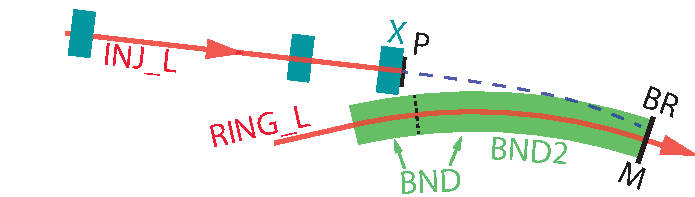
\includegraphics[width=5in]{injection.pdf}
  \caption[Injection line into a dipole magnet.]{Injection line into a dipole magnet.
  }
  \label{f:inject}
\end{figure}

An injection line is illustrated in \fig{f:inject}. In this example, The path of an injected
particle after it leaves the last element \vn{X} of the injection line (dashed blue line) partially
goes through the field of the dipole \vn{BND} in the storage ring. One way to simulate this is:
\begin{example}
  INJ_L: line = (..., X, P, BND2, BR)
  RING_L: line = (..., BND, M, ...)
  P: patch, x_offset = -0.5, x_pitch = 0.15, z_offset = 0.3 
  BND: sbend, l = 6.2, g = 1/52
  BND2: BND, l = 4.7, tracking_method = runge_kutta,
          field_calc = fieldmap, grid_field = \{...\}
  BR: fork, to_line = RING_L, to_element = M
  M: marker
  use, INJ_L
\end{example}

In order to properly track particles through the fringe field of the dipole \vn{BND}, a partial
section of \vn{BND}, called \vn{BND2}, is placed in the injection line \vn{INJ_L}. The
\vn{tracking_method} for \vn{BND2} is set to \vn{runge_kutta} since the default \vn{bmad_standard}
tracking is not able to handle these fringe fields. Additionally, the \vn{field_calc} parameter of
\vn{BND2} is set to \vn{field map} so that the actual field profile of this particular magnet can be
used in the tracking. The field is specified in the \vn{grid_field} parameter (\sref{s:fieldmap}).

After traversing element \vn{X} in the injection line, the particle goes through the patch \vn{P}
which offsets the reference trajectory so that the following element, \vn{BND2}, is properly positioned.
The beginning of \vn{BND2} is marked by a black dashed line in the figure.  At the end of \vn{BND2}
the fork element \vn{BR} connects \vn{INJ_L} with the marker \vn{M} in \vn{RING_L}.

%-----------------------------------------------------------------------------
\section{Example: Chicane}
\label{s:ex.chicane}

\begin{figure}[tb]
  \centering
  \includegraphics[width=5.5in]{chicane.pdf}
  \caption[Four bend chicane.]{Four bend chicane. A) Correctly implemented chicane. The red line is 
the beam orbit magnified by a factor of 100. B) Incorrectly implemented chicane where the \vn{g}
parameter of the bends is used to control the chicane strength instead of \vn{dg}.
  }
  \label{f:chicane}
\end{figure}

A \vn{chicane} is a series of bending magnets that shifts the beam trajectory in the transverse
plane while keeping the starting and ending trajectories constant. Chicanes are useful for doing
things like bunch compression or as a variable bunch time delay. An example four bend chicane is
illustrated in \fig{f:chicane}A. The lattice file for this is:
\begin{example}
  parameter[geometry] = open
  beginning[beta_a] = 20
  beginning[beta_b] = 20
  parameter[p0c] = 1e7

  bnd1: rbend, l = 2
  bnd2: rbend, l = 2
  d1: drift, l = 3
  d2: drift, l = 2

  chicane: overlay = {bnd1[dg]:-ge, bnd2[dg]:ge}, var = {ge}, ge = 2e-3

  c_line: line = (bnd1, d1, bnd2, d2, bnd2, d1, bnd1)
  use, c_line
\end{example}
The chicane is controlled by an overlay (\sref{s:overlay}) called \vn{chicane}. This overlay controls
the \vn{dg} attribute of the bends (alternatively the \vn{hkick} or \vn{b0} attributes could have
been used).

It is important to note that using \vn{g} instead of \vn{dg} to control the chicane strength
would be a mistake. [Or, alternatively, \vn{b_field} instead of \vn{db_field} if controlling the
unnormalized field.] This is illustrated in \fig{f:chicane}B where the chicane overlay was replaced
by:
\begin{example}
  chicane: overlay = {bnd1[g]:-ge, bnd2[g]:ge}, var = {ge}, ge = 1e-1
\end{example}
The problem here is that \vn{g} sets the reference orbit so varying \vn{g} will vary the physical
layout of the machine which is not what is wanted. Since the actual normalized field is \vn{g +
dg}, it is \vn{dg} that should be varied. Notice that in the case where \vn{g} is varied, the
bends are no longer rectangular. This is true since \vn{rbend} elements, when read in from the
lattice file, are converted to \vn{sbend} elements. In this case the converted bends have \vn{e1}
and \vn{e2} face angles of zero. When the \vn{chicane} overlay varies \vn{g}, the face angle remain
zero. That is, the bends will always be pure sector bends. [In a situation where, indeed, \vn{g} is
to be varied and it is desired to keep bends rectangular, the appropriate variation of the \vn{e1}
and \vn{e2} can be put in the controlling overlay.]

%-----------------------------------------------------------------------------
\section{Example: Energy Recovery Linac}
\label{s:ex.erl}

An Energy Recovery Linac (ERL) is illustrated in \fig{f:erl}A. The ERL starts with an injection line
that feeds a linac which accelerates the beam to some energy. The beam then transverses a return
\vn{arc} which reinjects the bunches into the linac. The length of the return arc is such that, on
the second pass, the beam is decelerated giving its energy back to the RF cavities. Finally, the
decelerated beam is steered through a dump line where, at the end, an absorber stops the beam.

 A lattice file for modeling this ERL:
\begin{example}
  parameter[geometry] = open
  bmad_com[absolute_time_tracking] = T

  BEND_L1: sbend, angle = -25*pi/180, l = 0.2, ...
  BEND_L2: BEND_L1

  A_PATCH: patch, flexible = T
  D_PATCH: patch, x_offset = 0.034, x_pitch = asin(0.32) 
  INJECT: line = (...)
  LINAC: line[multipass] = (BEND_L1, ..., BEND_L2)
  ARC: line = (..., BEND_A7)
  DUMP: line = (...)

  ERL: line = (INJECT, LINAC, ARC, A_PATCH, LINAC, D_PATCH, DUMP)
\end{example}

\begin{figure}[tb]
  \centering
  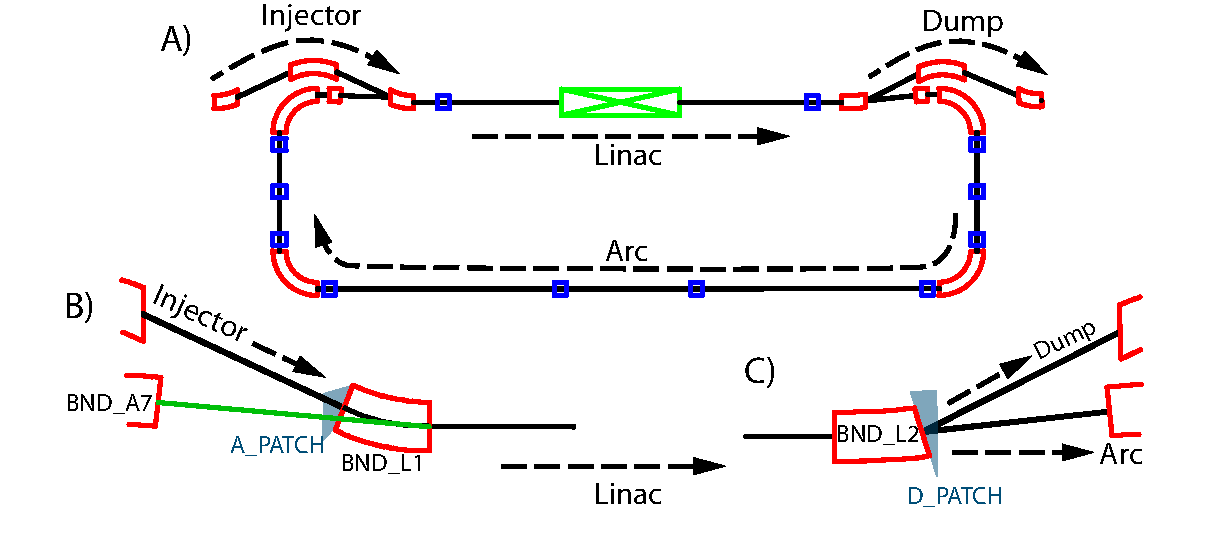
\includegraphics[width=6in]{erl.pdf}
  \caption[Example Energy Recovery Linac.]{
Example Energy Recovery Linac. A) The ERL consists of an injection line, accelerating linac, return
arc, deceleration linac, and finally a beam dump. B) Close up of the section where the end of the
injector and the end of the arc inject into the beginning of the linac. C) Close up of the end of
the linac which injects into the dump and the beginning of the arc.}
  \label{f:erl}
\end{figure}

\index{patch!example}
\fig{f:erl}B shows the injector and arc merging into the beginning of the linac. The first element
of the linac is a bend named \vn{BEND_L1}. The bending angle for \vn{BEND_L1} has been set at the
appropriate value for injection from the injector. To get the correct geometry for injection from
the arc, a \vn{patch} element, named \vn{A_PATCH}, is placed in the \vn{ERL} line between the arc
and the linac. \vn{A_PATCH} is a flexible patch which means that the exit edge of \vn{A_PATCH} will
automatically be aligned with the entrance edge of the next element which is \vn{BEND_L1}.

Note that this use of a flexible patch works since the orientation of \vn{BEND_L1} has been
determined before the orientation of \vn{A_PATCH} is determined. The orientation of elements is
determined in order starting from the first element in the line (the exception to this rule is if
there is a \vn{floor_position} element) and the orientation of \vn{BEND_L1} is thus determined right
after the injector section on the first pass through the linac.

\fig{f:erl}C shows the end of the linac splitting off into the dump and arc sections. The
\vn{D_PATCH} is used to orient the reference trajectory so that the dump is correctly positioned.
Here it is not possible to make the \vn{D_PATCH} flexible since the position of the dump is unknown
when the orientation of the \vn{D_PATCH} is calculated. However, the \vn{D_PATCH} could be made
flexible if a \vn{floor_position} element is used in the dump line (\bmad will work both forward and
backwards from a \vn{floor_position} element so that a \vn{floor_position} element may be placed
anywhere in the dump line).

%-----------------------------------------------------------------------------
\section{Example: Colliding Beam Storage Rings}
\label{s:ex.collide}

\begin{figure}[tb]
  \centering
  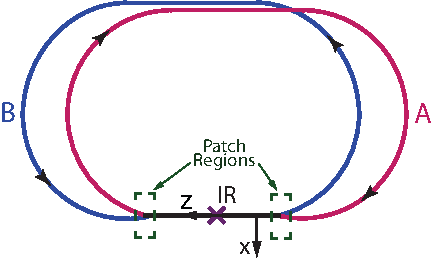
\includegraphics[width=5in]{colliding-beams.pdf}
  \caption[Dual ring colliding beam machine]{Dual ring colliding beam machine. 
The beam in the \vn{A} ring rotates clockwise and in the \vn{B} ring
counterclockwise.}
  \label{f:collide}
\end{figure}

The idealized layout of a pair of storage rings used for colliding
counter rotating beams of electrons and gold is shown in \fig{f:collide}. Rings \vn{A} and
\vn{B} intersect at two interaction regions labeled \vn{ir1} and
\vn{ir2} where the beams collide. The basic lattice description is:
\begin{example}
  ir: line[multipass] = (...)
  pa_in; patch, ... ;  pa_out; patch, ...
  pb_in; patch, ... ;  pb_out; patch, ...
  m: marker
  fid: fiducial, origin_ele = m
  ...
  A: line = (arc_a, pa_in, ir, m, pa_out)
  A[particle] = electron
  B_rev: line = (arc_b, pb_in, ir, fid, pb_out)
  B: line = (--B_rev)
  B[particle] = Au+79
  use, A, B
\end{example}
Lines \vn{ir} is the interaction region line which is
declared \vn{multipass} since they are shared by the two rings. Line
\vn{A} represents ring \vn{A}. In ring \vn{A} where the electron beam which, by definition,
travels in the same direction as increasing $s$, rotates clockwise.
Line \vn{B_rev} is a ``reversed'' line of ring \vn{B} and, like
\vn{a}, represents a beam rotating clockwise.  Line \vn{B}, which
represents ring \vn{B}, is the reverse of \vn{B_rev} and here the gold beam
rotates counterclockwise. In this construction, all elements of \vn{B}
are reversed.  While this is not mandatory (only the interaction
regions must be reversed in \vn{B}), having all of \vn{B} reversed
simplifies the geometry since this means that the local coordinate
systems of both lines \vn{A} and \vn{b} will be ``aligned'' with the
$x$-axis pointing to the outside of the ring and the $y$-axis pointing
up, out of the page. Having non-aligned coordinate systems is possible
but potentially very confusing.

The two rings are physically aligned using a marker \vn{m} in \vn{A}
and a \vn{fiducial} element \vn{fid} in \vn{B} that aligns with
\vn{m}.  Each ring has two rigid \vn{patch} elements, \vn{pa_in} and \vn{pa_out} for the \vn{A}
ring, and \vn{pb_in} and \vn{bp_out} for the \vn{B} ring, on either side of the interaction region.
The dashed, green rectangles in the figure show the regions where the patches are.

The finished lattice will have two branches, The first branch (with
index 0) will be derived from line \vn{A} (and hence will be named
``A'') and the second branch (with index 1) will be derived from line
\vn{B} (and hence will be named ``B''). The multipass lords
representing the physical IR elements will be in the ``lord section''
of branch 0.



\begin{figure}[tb]
  \centering
  \includegraphics[width=5in]{rowland-circle.pdf}
  \caption[Rowland circle spectrometer]
  {
Rowland circle spectrometer: A) X-rays scattered from a sample (labeled source in the figure)
illuminates a crystal with X-rays. Some of the X-rays are reflected from the crystal onto the
detector. Note: For clarity's sake the center of the global coordinate system as shown is shifted
from the true center at the Source element. B) The detector image when the radius of curvature of
the bent crystal is ``perfect''. That is, twice the radius of the Rowland circle. C) The detector
image when the radius of curvature of the crystal is shifted 1\% from perfect.
  }
  \label{f:rowland}
\end{figure}

%-----------------------------------------------------------------------------
\section{Example: Rowland Circle X-Ray Spectrometer}
\label{s:rowland}

This example shows how \bmad can be used to simulate X-rays. In this case, the present example is
taken from a case study where simulations were done in order to understand how imperfections in a Rowland
circle spectrometer would affect measurements.

A Rowland circle spectrometer is illustrated in \fig{f:rowland}A. The \vn{source} was
a sample that is illuminated with X-rays. Some of the X-rays scatter from the \vn{sample} and are
reflected from the \vn{crystal} to the \vn{detector}. To properly focus the X-rays onto the
\vn{detector}, the \vn{source}, \vn{crystal} and \vn{detector} lie on a circle, called the Rowland
circle. The \vn{crystal} is bent and the radius of curvature of the crystal is
$2R$ where $R$ is the radius of the Rowland circle.

The angle from the \vn{source} to the Rowland circle center to the crystal is
$2\theta_\text{B,in}-\phi$ where $\theta_\text{B,in}$ is the entrance Bragg angle for photons whose
energy matches the given reference energy and $\phi$ is an angle that will be varied when doing an energy
scan of the scattered X-ray spectrum. Similarly, the angle from the \vn{crystal} to the Rowland
circle center to the \vn{detector} is $2\theta_\text{B,out}-\phi$ where $\theta_\text{B,out}$ is the
exit Bragg angle at the given reference energy.

The lattice for this simulation is:
\begin{example}
  beginning[e_tot] = 8.955e3    ! Reference photon energy
  parameter[particle] = photon

  phi = 0
  err = 0
  r_rowland = 0.5               ! Rowland circle radius

  source: photon_init, sig_x = 5e-5, sig_y = 5e-5, spatial_distribution = uniform,
          E_center_relative_to_ref = T, sig_E = 2, energy_distribution = gaussian,
          velocity_distribution = spherical

  drift1: drift

  cryst: crystal, crystal_type = "Si(553)", b_param = -1, aperture = 0.050,
  	curvature = \{spherical = (1+err) / (2 * r_rowland)\}, aperture_type = elliptical

  drift2: drift

  det: detector, pixel = \{ix_bounds = (-97, 97), 
                                    iy_bounds = (-243, 243), dr = (172e-6, 172e-6)\}

  daves_line: line = (source, drift1, cryst, drift2, det)
  use, daves_line

  !------------------

  expand_lattice ! Calculates the Bragg angles needed below.

  theta_in  = cryst[bragg_angle_in]  ! 78.2759 * pi / 180
  theta_out = cryst[bragg_angle_out] ! 78.2759 * pi / 180

  cryst[graze_angle_in]  = theta_in - phi/2 
  cryst[graze_angle_out] = theta_out - phi/2
  drift1[L] = 2 * r_rowland * sin(theta_in-phi/2)
  drift2[L] = 2 * r_rowland * sin(theta_out-phi/2)

  beginning[theta_position] = theta_in + phi/2
  det[x_pitch] = pi/2 - theta_out + phi/2
\end{example}

The reference photon energy is 8.995~KeV and the Rowland circle radius is 0.5~m. The simulation uses
a \vn{photon_init} element (\sref{s:photon.init}) for the \vn{source} having a Gaussian energy
spread with a sigma of 2~eV.  The initial velocity distribution of the photons, set by the
\vn{velocity_distribution} parameter, is taken to be uniform in all directions (``\vn{spherical}''
distribution). Since the element that is downstream from the source (which is the crystal element)
has a defined aperture, \bmad is able to use this to not generate photons that will be lost at the
crystal. This reduces the simulation time.

The crystal is \vn{Silicon} 553 crystal which is symmetrically cut (\vn{b_param} = -1) so that in
this example the entrance Bragg angle is equal to the exit Bragg angle.  The detector has a
segmented surface with pixels spaced 172$\mu$m apart. Along the $x$-axis, which is the coordinate
along the detector surface in the plane of \fig{f:rowland}A, the pixel index is in the range $[-97,
97]$. Along the $y$-axis, which is the out of plane coordinate, the pixel index is in the range
$[-243,243]$.

The \vn{expand_lattice} command (\sref{s:expand.lat}) is used to command \bmad to construct the
lattice which includes calculating the Bragg angles. After lattice expansion, the variables
\vn{theta_in} and \vn{theta_out} are set to the Bragg angle entrance and exit Bragg angles
respectively. The entrance and exit graze angles of the crystal, which are used to determine the
reference trajectory (\sref{s:mirror.coords}), can be set to \vn{theta_in - phi} and \vn{theta_out -
phi} respectively. Note that if these graze angles had not been explicitly set, the graze angles
would be automatically set to the Bragg angles which
is not what is wanted when doing an energy scan with finite \vn{phi}.

In the actual experimental setup that this example is modeled on, the source and Rowland circle were
fixed in the global coordinate system (\sref{s:global}) while the crystal and detector move with
changing \vn{phi} (see \fig{f:rowland}A). To mimic this, the \vn{beginning[theta_position]}
(\sref{s:beginning}) is set to give the desired orientation of the beginning reference trajectory
within the global coordinate system. This does not affect photon tracking since changing the initial
orientation of the reference trajectory just shifts all the lattice elements as one rigid
body. Additionally, the detector orientation is fixed so that the detector surface normal always
points towards the Rowland circle center. To get the correct orientation for the detector, the
detector's \vn{x_pitch} attribute, which rotates the detector (\sref{s:offset}), is set appropriately.

The effect of varying the \vn{crystal} curvature is shown in \fig{f:rowland}B and
\fig{f:rowland}C. A \bmad based program called \vn{Lux} was used for the simulation. The \vn{Lux}
program generates a set of photons and records the statistics at the detector. In \fig{f:rowland}B
the \vn{crystal} is correctly bent with the parameter \vn{err} in the lattice set to zero. This
produces a well focused spot on the \vn{detector}. In \fig{f:rowland}C the \vn{crystal} curvature
is shifted by 1\% by setting \vn{err} equal to 0.01. This error degrades the focusing and leads to a
spot that is enlarged along the $x$-axis.


%-----------------------------------------------------------------------------
\section{Example: Backward Tracking Through a Lattice}
\label{s:reverse}

By creating a reversed lattice, one can track a particles backwards through the lattice. For
example, assume that you have a lattice file called \vn{original_lattice.bmad} which defines a line
called \vn{original_line} tracking electrons. To create a reversed lattice, create a new file with
the following:
\begin{example}
  call, file = original_lattice.bmad
  reversed_line: line = (--original_line)
  parameter[default_tracking_species] = positron
  use, reversed_line
\end{example}
The ``$--$'' reverses the line and reverses the elements (\sref{s:ele.reverse}). Tracking
through \vn{reversed_line} is equivalent to tracking backwards through \vn{original_line}.

The default for the type of particle tracked is set by \vn{parameter[default_tracking_species]}
(\sref{s:param}). [A \bmad based program can always override this default but it will be assumed
here that this is not the case.] In this case, the default species to use for tracking is set to the
antiparticle of the reference particle species. If the \vn{original_line} lattice had just static
magnetic fields and no electric fields, by tracking with the anti-particle in the reversed lattice,
the anti-particle will follow the same path (but backward) as the particle in the original
lattice. For this to work, the anti-particle must be started with the appropriate phase space
coordinates. If $(x, p_x, y, p_y, z, p_z)$ is the phase space coordinates of the particle at the end
of the original lattice, the anti-particle must be initialized with phase space coordinates of $(x,
-p_x, y, -p_y, \text{immaterial}, p_z)$.

It should be keept in mind that tracking backwards in the lattice is not exactly the same as
tracking backwards in time. In particular, the two are different if there are electric fields or if
radiation damping and/or excitation is turned on.

\chapter{Lattice File Conversion}
\label{c:lat.convert}
\index{conversion to other lattice formats}

A \bmad Distribution (\sref{s:tao.intro}) contains a number of translation programs between \bmad
and other formats.


%-----------------------------------------------------------------------------
\section{MAD Conversion}
\label{s:mad.convert}
\index{MAD!conversion}

%-----------------------------------------------------------------------------
\subsection{Convert MAD to Bmad}
\label{s:mad.bmad.uap}

Python scripts to convert from MAD8 and MADX are available at:
\begin{example}
  util_programs/mad_to_bmad
\end{example}
Due to differences in language definitions, conversions must be done with some care. The following
differences should be noted:
  \begin{itemize}
  \item
\bmad, unlike \mad, does not have any ``action'' commands. An action command is a command that makes
a calculation. Examples include \mad's \vn{SURVEY} and \vn{TWISS} commands.
  \item
In \bmad all variables must be defined before being used (\sref{s:arith}) while \mad will simply take
a variable's value to be zero if it is not defined.
  \item
\bmad, unlike \mad, does not allow variable values to be redefined.
  \end{itemize}

%-----------------------------------------------------------------------------
\subsection{Convert Bmad to MAD}
\label{s:bmad.mad}

\index{wiggler!conversion to MAD}
\index{sol_quad!conversion to MAD}
To convert to MAD8 or MADX, the \tao program can be used. Additionally, there is the program
\begin{example}
  util_programs/bmad_to_mad_sad_elegant
\end{example}
Since \mad does not have a \vn{wiggler} or a
\vn{sol_quad} element, this conversion routine makes ``equivalent'' substitution. For a
\vn{sol_quad}, the equivalent substitution will be a drift-matrix-drift series of elements. For a
\vn{wiggler}, a series of bend and drift elements will be used (the program can also use a
drift-matrix-drift model here but that is not as accurate). The bends and drifts for the
\vn{wiggler} model are constructed so that the global geometry of the lattice does not
change. Additionally the bends and drifts are constructed to most nearly match the wiggler's
\begin{example}
  Transfer matrix
  $I_2$ and $I_3$ synchrotron radiation integrals (\sref{s:synch.ints})
\end{example}
Note that the resulting model will not have the vertical cubic nonlinearity that the actual wiggler
has.

%-----------------------------------------------------------------------------
\section{Convert to PTC}
\label{s:to.ptc}

A PTC ``\vn{flatfile}'' can be constructed using the \tao program with the following commands:
\begin{example}
  Tao> ptc init
  Tao> write ptc
\end{example}

%---------------------------------------------------------------------------
\section{SAD Conversion}
\label{s:sad.convert}
\index{SAD}

Conversion from \vn{SAD}\cite{b:sad} to \bmad is accomplished using the Python script
\begin{example}
  util_programs/sad_to_bmad/sad_to_bmad.py
\end{example}
Currently, the following restrictions on SAD lattices apply:
  \begin{itemize}
  \item
SAD \vn{mult} elements cannot have an associated RF field
  \item
Misalignments in a \vn{sol} element with \vn{geo} = 1 cannot be handled.
  \end{itemize}

\bmad to \vn{SAD} to conversion can be done with the \tao program or the program 
\begin{example}
  util_programs/bmad_to_mad_sad_elegant
\end{example}

%---------------------------------------------------------------------------
\section{Elegant Conversion}
\label{s:elegant.convert}
\index{Elegant}

Conversion from \vn{Elegant}\cite{b:elegant} to \bmad is accomplished using the Python script
\begin{example}
  util_programs/elegant_to_bmad/elegant_to_bmad.py
\end{example}

\bmad to \vn{Elegant} to conversion can be done with the \tao program or the program 
\begin{example}
  util_programs/bmad_to_mad_sad_elegant
\end{example}

%---------------------------------------------------------------------------
\section{Astra, Blender, CSRTrack, GPT, and Merlin Conversion}
\label{s:other.convert}
\index{Astra}\index{Blender}\index{CSRTrack}\index{GPT}\index{Merlin}

Conversion programs to Astra, Blender, CSRTrack, GPT, and Merlin exist in the \vn{util_programs}
directory. Some conversion code is still in beta development so if you encounter
problems please contact a \bmad maintainer. 

\chapter{List of Element Attributes}
\label{c:attrib.list}

Alphabetical list of element attributes for each type of element. 

Note for programmers: The program that generates a file of attributes indexed by the
internal reference number is:
\begin{example}
  util_programs/element_attributes.f90 
\end{example}

 %---------------------------------
 \section{AB_multipoleAttributes}
 \label{s:list.ab.multipole}
 
 \begin{tabular}{lll} \toprule
a0 - a20, b0 - b20          & mat6_calc_method            & type                        \\
alias                       & multipoles_on               & wall                        \\
aperture                    & offset                      & x1_limit                    \\
aperture_at                 & offset_moves_aperture       & x2_limit                    \\
aperture_type               & p0c                         & x_limit                     \\
accordion_edge              & ptc_integration_type        & x_offset                    \\
create_jumbo_slave          & reference                   & x_offset_tot                \\
delta_ref_time              & ref_origin                  & y1_limit                    \\
descrip                     & spin_tracking_method        & y2_limit                    \\
ele_origin                  & superimpose                 & y_limit                     \\
e_tot                       & s_position                  & y_offset                    \\
end_edge                    & start_edge                  & y_offset_tot                \\
field_master                & tilt                        & z_offset                    \\
is_on                       & tilt_tot                    & z_offset_tot                \\
l                           & tracking_method             &                             \\
 \bottomrule
 \end{tabular}
 \vfill
 
 %---------------------------------
 \section{BeamBeamAttributes}
 \label{s:list.beambeam}
 
 \begin{tabular}{lll} \toprule
alias                       & field_calc                  & tracking_method             \\
alpha_a                     & is_on                       & type                        \\
alpha_b                     & l                           & wall                        \\
aperture                    & mat6_calc_method            & x1_limit                    \\
aperture_at                 & n_slice                     & x2_limit                    \\
aperture_type               & n_slice                     & x_limit                     \\
bbi_constant                & offset                      & x_offset                    \\
beta_a                      & offset_moves_aperture       & x_offset_tot                \\
beta_b                      & p0c                         & x_pitch                     \\
charge                      & ptc_integration_type        & x_pitch_tot                 \\
cmat_11                     & reference                   & y1_limit                    \\
cmat_12                     & ref_origin                  & y2_limit                    \\
cmat_21                     & sig_x                       & y_limit                     \\
cmat_22                     & sig_y                       & y_offset                    \\
create_jumbo_slave          & sig_z                       & y_offset_tot                \\
delta_ref_time              & spin_tracking_method        & y_pitch                     \\
descrip                     & superimpose                 & y_pitch_tot                 \\
ele_origin                  & tilt                        & z_offset                    \\
e_tot                       & tilt_tot                    & z_offset_tot                \\
 \bottomrule
 \end{tabular}
 \vfill
 
 %---------------------------------
 \section{Bend_Sol_QuadAttributes}
 \label{s:list.bend.sol.quad}
 
 \begin{tabular}{lll} \toprule
a0 - a20, b0 - b20          & hkick                       & superimpose                 \\
alias                       & integrator_order            & symplectify                 \\
angle                       & is_on                       & s_position                  \\
aperture                    & k1                          & start_edge                  \\
aperture_at                 & ks                          & taylor_field                \\
aperture_type               & l                           & taylor_map_includes_offsets \\
accordion_edge              & lord_pad1                   & tilt                        \\
b1_gradient                 & lord_pad2                   & tilt_tot                    \\
bend_tilt                   & lr_freq_spread              & tracking_method             \\
bl_hkick                    & lr_self_wake_on             & type                        \\
bl_vkick                    & lr_wake_file                & vkick                       \\
bs_field                    & lr_wake_spline              & wall                        \\
b_field                     & l_hard_edge                 & x1_limit                    \\
cartesian_map               & mat6_calc_method            & x2_limit                    \\
create_jumbo_slave          & multipoles_on               & x_limit                     \\
csr_calc_on                 & num_steps                   & x_offset                    \\
cylindrical_map             & n_ref_pass                  & x_offset_tot                \\
delta_ref_time              & offset                      & x_pitch                     \\
descrip                     & offset_moves_aperture       & x_pitch_tot                 \\
dks_ds                      & p0c                         & x_quad                      \\
ds_step                     & ptc_integration_type        & y1_limit                    \\
ele_origin                  & quad_tilt                   & y2_limit                    \\
e_tot                       & r0_elec                     & y_limit                     \\
end_edge                    & r0_mag                      & y_offset                    \\
field_calc                  & reference                   & y_offset_tot                \\
field_master                & ref_origin                  & y_pitch                     \\
field_overlaps              & rho                         & y_pitch_tot                 \\
fringe_at                   & scale_multipoles            & y_quad                      \\
fringe_type                 & spin_fringe_on              & z_offset                    \\
g                           & spin_tracking_method        & z_offset_tot                \\
grid_field                  & sr_wake_file                &                             \\
 \bottomrule
 \end{tabular}
 \vfill
 
 %---------------------------------
 \section{CapillaryAttributes}
 \label{s:list.capillary}
 
 \begin{tabular}{lll} \toprule
alias                       & p0c                         & x_offset                    \\
aperture                    & ptc_integration_type        & x_offset_tot                \\
aperture_at                 & reference                   & x_pitch                     \\
aperture_type               & ref_origin                  & x_pitch_tot                 \\
create_jumbo_slave          & spin_tracking_method        & y1_limit                    \\
critical_angle_factor       & superimpose                 & y2_limit                    \\
delta_ref_time              & s_spline                    & y_limit                     \\
descrip                     & tilt                        & y_offset                    \\
ele_origin                  & tilt_tot                    & y_offset_tot                \\
e_tot                       & tracking_method             & y_pitch                     \\
l                           & type                        & y_pitch_tot                 \\
mat6_calc_method            & wall                        & z_offset                    \\
n_slice_spline              & x1_limit                    & z_offset_tot                \\
offset                      & x2_limit                    &                             \\
offset_moves_aperture       & x_limit                     &                             \\
 \bottomrule
 \end{tabular}
 \vfill
 
 %---------------------------------
 \section{CrystalAttributes}
 \label{s:list.crystal}
 
 \begin{tabular}{lll} \toprule
alias                       & mat6_calc_method            & tracking_method             \\
alpha_angle                 & offset                      & type                        \\
aperture                    & offset_moves_aperture       & v_unitcell                  \\
aperture_at                 & p0c                         & wall                        \\
aperture_type               & pendellosung_period_pi      & x1_limit                    \\
bragg_angle                 & pendellosung_period_sigma   & x2_limit                    \\
bragg_angle_in              & psi_angle                   & x_limit                     \\
bragg_angle_out             & ptc_integration_type        & x_offset                    \\
b_param                     & reference                   & x_offset_tot                \\
create_jumbo_slave          & ref_cap_gamma               & x_pitch                     \\
crystal_type                & ref_orbit_follows           & x_pitch_tot                 \\
curvature_x0_y2             & ref_origin                  & y1_limit                    \\
darwin_width_pi             & ref_tilt                    & y2_limit                    \\
darwin_width_sigma          & ref_tilt_tot                & y_limit                     \\
dbragg_angle_de             & ref_wavelength              & y_offset                    \\
delta_ref_time              & spin_tracking_method        & y_offset_tot                \\
descrip                     & superimpose                 & y_pitch                     \\
diffraction_limited         & surface                     & y_pitch_tot                 \\
d_spacing                   & thickness                   & z_offset                    \\
ele_origin                  & tilt                        & z_offset_tot                \\
e_tot                       & tilt_corr                   &                             \\
l                           & tilt_tot                    &                             \\
 \bottomrule
 \end{tabular}
 \vfill
 
 %---------------------------------
 \section{CustomAttributes}
 \label{s:list.custom}
 
 \begin{tabular}{lll} \toprule
alias                       & lr_wake_spline              & val12                       \\
aperture                    & l_hard_edge                 & val2                        \\
aperture_at                 & mat6_calc_method            & val3                        \\
aperture_type               & num_steps                   & val4                        \\
accordion_edge              & n_ref_pass                  & val5                        \\
create_jumbo_slave          & offset                      & val6                        \\
csr_calc_on                 & offset_moves_aperture       & val7                        \\
delta_e                     & p0c                         & val8                        \\
delta_ref_time              & p0c_start                   & val9                        \\
descrip                     & ptc_integration_type        & wall                        \\
ds_step                     & reference                   & x1_limit                    \\
ele_origin                  & ref_origin                  & x2_limit                    \\
e_tot                       & spin_tracking_method        & x_limit                     \\
e_tot_start                 & sr_wake_file                & x_offset                    \\
end_edge                    & superimpose                 & x_offset_tot                \\
field_calc                  & symplectify                 & x_pitch                     \\
field_master                & s_position                  & x_pitch_tot                 \\
field_overlaps              & start_edge                  & y1_limit                    \\
integrator_order            & taylor_map_includes_offsets & y2_limit                    \\
is_on                       & tilt                        & y_limit                     \\
l                           & tilt_tot                    & y_offset                    \\
lord_pad1                   & tracking_method             & y_offset_tot                \\
lord_pad2                   & type                        & y_pitch                     \\
lr_freq_spread              & val1                        & y_pitch_tot                 \\
lr_self_wake_on             & val10                       & z_offset                    \\
lr_wake_file                & val11                       & z_offset_tot                \\
 \bottomrule
 \end{tabular}
 \vfill
 
 %---------------------------------
 \section{DetectorAttributes}
 \label{s:list.detector}
 
 \begin{tabular}{lll} \toprule
alias                       & offset_moves_aperture       & x_limit                     \\
aperture                    & osc_amplitude               & x_offset                    \\
aperture_at                 & p0c                         & x_offset_calib              \\
aperture_type               & ptc_integration_type        & x_offset_tot                \\
create_jumbo_slave          & reference                   & x_pitch                     \\
crunch                      & ref_origin                  & x_pitch_tot                 \\
crunch_calib                & spin_tracking_method        & y1_limit                    \\
curvature_x0_y2             & superimpose                 & y2_limit                    \\
delta_ref_time              & surface                     & y_gain_calib                \\
descrip                     & tilt                        & y_gain_err                  \\
de_eta_meas                 & tilt_calib                  & y_limit                     \\
ele_origin                  & tilt_tot                    & y_offset                    \\
e_tot                       & tracking_method             & y_offset_calib              \\
is_on                       & type                        & y_offset_tot                \\
l                           & wall                        & y_pitch                     \\
mat6_calc_method            & x1_limit                    & y_pitch_tot                 \\
noise                       & x2_limit                    & z_offset                    \\
n_sample                    & x_gain_calib                & z_offset_tot                \\
offset                      & x_gain_err                  &                             \\
 \bottomrule
 \end{tabular}
 \vfill
 
 %---------------------------------
 \section{Diffraction_PlateAttributes}
 \label{s:list.diffraction.plate}
 
 \begin{tabular}{lll} \toprule
alias                       & p0c                         & x_offset                    \\
aperture                    & ptc_integration_type        & x_offset_tot                \\
aperture_at                 & reference                   & x_pitch                     \\
aperture_type               & ref_origin                  & x_pitch_tot                 \\
create_jumbo_slave          & ref_wavelength              & y1_limit                    \\
curvature_x0_y2             & spin_tracking_method        & y2_limit                    \\
delta_ref_time              & superimpose                 & y_limit                     \\
descrip                     & surface                     & y_offset                    \\
ele_origin                  & tilt                        & y_offset_tot                \\
e_tot                       & tilt_tot                    & y_pitch                     \\
field_scale_factor          & tracking_method             & y_pitch_tot                 \\
is_on                       & type                        & z_offset                    \\
mat6_calc_method            & wall                        & z_offset_tot                \\
mode                        & x1_limit                    & l                           \\
offset                      & x2_limit                    &                             \\
offset_moves_aperture       & x_limit                     &                             \\
 \bottomrule
 \end{tabular}
 \vfill
 
 %---------------------------------
 \section{DriftAttributes}
 \label{s:list.drift}
 
 \begin{tabular}{lll} \toprule
alias                       & num_steps                   & wall                        \\
aperture                    & n_ref_pass                  & x1_limit                    \\
aperture_at                 & offset                      & x2_limit                    \\
aperture_type               & offset_moves_aperture       & x_limit                     \\
accordion_edge              & p0c                         & x_offset                    \\
create_jumbo_slave          & ptc_integration_type        & x_offset_tot                \\
csr_calc_on                 & reference                   & x_pitch                     \\
delta_ref_time              & ref_origin                  & x_pitch_tot                 \\
descrip                     & spin_tracking_method        & y1_limit                    \\
ds_step                     & superimpose                 & y2_limit                    \\
ele_origin                  & symplectify                 & y_limit                     \\
e_tot                       & s_position                  & y_offset                    \\
end_edge                    & start_edge                  & y_offset_tot                \\
integrator_order            & taylor_map_includes_offsets & y_pitch                     \\
l                           & tilt                        & y_pitch_tot                 \\
lord_pad1                   & tilt_tot                    & z_offset                    \\
lord_pad2                   & tracking_method             & z_offset_tot                \\
mat6_calc_method            & type                        &                             \\
 \bottomrule
 \end{tabular}
 \vfill
 
 %---------------------------------
 \section{Collimators: Ecollimator and Rcollimator Attributes}
 \label{s:list.collimator}
 
 \begin{tabular}{lll} \toprule
alias                       & lord_pad2                   & tilt                        \\
aperture                    & lr_freq_spread              & tilt_tot                    \\
aperture_at                 & lr_self_wake_on             & tracking_method             \\
aperture_type               & lr_wake_file                & type                        \\
accordion_edge              & lr_wake_spline              & vkick                       \\
bl_hkick                    & l_hard_edge                 & wall                        \\
bl_vkick                    & mat6_calc_method            & x1_limit                    \\
create_jumbo_slave          & num_steps                   & x2_limit                    \\
csr_calc_on                 & n_ref_pass                  & x_limit                     \\
delta_ref_time              & offset                      & x_offset                    \\
descrip                     & offset_moves_aperture       & x_offset_tot                \\
ds_step                     & p0c                         & x_pitch                     \\
ele_origin                  & ptc_integration_type        & x_pitch_tot                 \\
e_tot                       & reference                   & y1_limit                    \\
end_edge                    & ref_origin                  & y2_limit                    \\
field_overlaps              & spin_fringe_on              & y_limit                     \\
fringe_at                   & spin_tracking_method        & y_offset                    \\
fringe_type                 & sr_wake_file                & y_offset_tot                \\
hkick                       & superimpose                 & y_pitch                     \\
integrator_order            & symplectify                 & y_pitch_tot                 \\
is_on                       & s_position                  & z_offset                    \\
l                           & start_edge                  & z_offset_tot                \\
lord_pad1                   & taylor_map_includes_offsets &                             \\
 \bottomrule
 \end{tabular}
 \vfill
 
 %---------------------------------
 \section{ELseparatorAttributes}
 \label{s:list.elseparator}
 
 \begin{tabular}{lll} \toprule
a0 - a20, b0 - b20          & l                           & start_edge                  \\
alias                       & lord_pad1                   & taylor_field                \\
aperture                    & lord_pad2                   & taylor_map_includes_offsets \\
aperture_at                 & lr_freq_spread              & tilt                        \\
aperture_type               & lr_self_wake_on             & tilt_tot                    \\
accordion_edge              & lr_wake_file                & tracking_method             \\
cartesian_map               & lr_wake_spline              & type                        \\
create_jumbo_slave          & l_hard_edge                 & vkick                       \\
csr_calc_on                 & mat6_calc_method            & voltage                     \\
cylindrical_map             & multipoles_on               & wall                        \\
delta_ref_time              & num_steps                   & x1_limit                    \\
descrip                     & n_ref_pass                  & x2_limit                    \\
ds_step                     & offset                      & x_limit                     \\
ele_origin                  & offset_moves_aperture       & x_offset                    \\
e_field                     & p0c                         & x_offset_tot                \\
e_tot                       & ptc_integration_type        & x_pitch                     \\
end_edge                    & r0_elec                     & x_pitch_tot                 \\
field_calc                  & r0_mag                      & y1_limit                    \\
field_master                & reference                   & y2_limit                    \\
field_overlaps              & ref_origin                  & y_limit                     \\
fringe_at                   & scale_multipoles            & y_offset                    \\
fringe_type                 & spin_fringe_on              & y_offset_tot                \\
gap                         & spin_tracking_method        & y_pitch                     \\
grid_field                  & sr_wake_file                & y_pitch_tot                 \\
hkick                       & superimpose                 & z_offset                    \\
integrator_order            & symplectify                 & z_offset_tot                \\
is_on                       & s_position                  &                             \\
 \bottomrule
 \end{tabular}
 \vfill
 
 %---------------------------------
 \section{EM_FieldAttributes}
 \label{s:list.em.field}
 
 \begin{tabular}{lll} \toprule
alias                       & l                           & symplectify                 \\
aperture                    & lord_pad1                   & s_position                  \\
aperture_at                 & lord_pad2                   & start_edge                  \\
aperture_type               & lr_freq_spread              & taylor_field                \\
autoscale_amplitude         & lr_self_wake_on             & taylor_map_includes_offsets \\
autoscale_phase             & lr_wake_file                & tilt                        \\
accordion_edge              & lr_wake_spline              & tilt_tot                    \\
cartesian_map               & l_hard_edge                 & tracking_method             \\
create_jumbo_slave          & mat6_calc_method            & type                        \\
csr_calc_on                 & num_steps                   & wall                        \\
cylindrical_map             & n_ref_pass                  & x1_limit                    \\
delta_ref_time              & offset                      & x2_limit                    \\
descrip                     & offset_moves_aperture       & x_limit                     \\
ds_step                     & p0c                         & x_offset                    \\
ele_origin                  & p0c_start                   & x_offset_tot                \\
e_tot                       & phi0                        & x_pitch                     \\
e_tot_start                 & phi0_autoscale              & x_pitch_tot                 \\
end_edge                    & phi0_err                    & y1_limit                    \\
field_autoscale             & ptc_integration_type        & y2_limit                    \\
field_calc                  & reference                   & y_limit                     \\
field_overlaps              & ref_origin                  & y_offset                    \\
fringe_at                   & rf_frequency                & y_offset_tot                \\
fringe_type                 & spin_fringe_on              & y_pitch                     \\
grid_field                  & spin_tracking_method        & y_pitch_tot                 \\
integrator_order            & sr_wake_file                & z_offset                    \\
is_on                       & superimpose                 & z_offset_tot                \\
 \bottomrule
 \end{tabular}
 \vfill
 
 %---------------------------------
 \section{E_GunAttributes}
 \label{s:list.e.gun}
 
 \begin{tabular}{lll} \toprule
alias                       & l                           & start_edge                  \\
aperture                    & lord_pad1                   & taylor_field                \\
aperture_at                 & lord_pad2                   & taylor_map_includes_offsets \\
aperture_type               & lr_freq_spread              & tilt                        \\
autoscale_amplitude         & lr_self_wake_on             & tilt_tot                    \\
autoscale_phase             & lr_wake_file                & tracking_method             \\
accordion_edge              & lr_wake_spline              & type                        \\
cartesian_map               & l_hard_edge                 & voltage                     \\
create_jumbo_slave          & mat6_calc_method            & voltage_err                 \\
csr_calc_on                 & num_steps                   & wall                        \\
cylindrical_map             & n_ref_pass                  & x1_limit                    \\
delta_ref_time              & offset                      & x2_limit                    \\
descrip                     & offset_moves_aperture       & x_limit                     \\
ds_step                     & p0c                         & x_offset                    \\
ele_origin                  & phi0                        & x_offset_tot                \\
e_tot                       & phi0_autoscale              & x_pitch                     \\
end_edge                    & phi0_err                    & x_pitch_tot                 \\
field_autoscale             & ptc_integration_type        & y1_limit                    \\
field_calc                  & reference                   & y2_limit                    \\
field_overlaps              & ref_origin                  & y_limit                     \\
fringe_at                   & rf_frequency                & y_offset                    \\
fringe_type                 & spin_fringe_on              & y_offset_tot                \\
gradient                    & spin_tracking_method        & y_pitch                     \\
gradient_err                & sr_wake_file                & y_pitch_tot                 \\
grid_field                  & superimpose                 & z_offset                    \\
integrator_order            & symplectify                 & z_offset_tot                \\
is_on                       & s_position                  &                             \\
 \bottomrule
 \end{tabular}
 \vfill
 
 %---------------------------------
 \section{FiducialAttributes}
 \label{s:list.fiducial}
 
 \begin{tabular}{lll} \toprule
alias                       & dz_origin                   & p0c                         \\
delta_ref_time              & ele_origin                  & ptc_integration_type        \\
descrip                     & e_tot                       & reference                   \\
dphi_origin                 & l                           & ref_origin                  \\
dpsi_origin                 & mat6_calc_method            & spin_tracking_method        \\
dtheta_origin               & offset                      & superimpose                 \\
dx_origin                   & origin_ele                  & tracking_method             \\
dy_origin                   & origin_ele_ref_pt           & type                        \\
 \bottomrule
 \end{tabular}
 \vfill
 
 %---------------------------------
 \section{Floor_ShiftAttributes}
 \label{s:list.floor.shift}
 
 \begin{tabular}{lll} \toprule
alias                       & offset                      & type                        \\
aperture                    & offset_moves_aperture       & upstream_ele_dir            \\
aperture_at                 & origin_ele                  & wall                        \\
aperture_type               & origin_ele_ref_pt           & x1_limit                    \\
accordion_edge              & p0c                         & x2_limit                    \\
create_jumbo_slave          & ptc_integration_type        & x_limit                     \\
delta_ref_time              & reference                   & x_offset                    \\
descrip                     & ref_origin                  & x_pitch                     \\
downstream_ele_dir          & spin_tracking_method        & y1_limit                    \\
ele_origin                  & superimpose                 & y2_limit                    \\
e_tot                       & s_position                  & y_limit                     \\
end_edge                    & start_edge                  & y_offset                    \\
l                           & tilt                        & y_pitch                     \\
mat6_calc_method            & tracking_method             & z_offset                    \\
 \bottomrule
 \end{tabular}
 \vfill
 
 %---------------------------------
 \section{Fork and Photon_Fork Attributes}
 \label{s:list.fork}
 
 \begin{tabular}{lll} \toprule
alias                       & ix_to_element               & to_element                  \\
aperture                    & l                           & to_line                     \\
aperture_at                 & mat6_calc_method            & tracking_method             \\
aperture_type               & new_branch                  & type                        \\
create_jumbo_slave          & offset                      & x1_limit                    \\
delta_ref_time              & offset_moves_aperture       & x2_limit                    \\
descrip                     & p0c                         & x_limit                     \\
direction                   & ptc_integration_type        & y1_limit                    \\
ele_origin                  & reference                   & y2_limit                    \\
e_tot                       & ref_origin                  & y_limit                     \\
is_on                       & spin_tracking_method        &                             \\
ix_to_branch                & superimpose                 &                             \\
 \bottomrule
 \end{tabular}
 \vfill
 
 %---------------------------------
 \section{GirderAttributes}
 \label{s:list.girder}
 
 \begin{tabular}{lll} \toprule
alias                       & l                           & x_offset_tot                \\
descrip                     & origin_ele                  & x_pitch                     \\
dphi_origin                 & origin_ele_ref_pt           & x_pitch_tot                 \\
dpsi_origin                 & ref_tilt                    & y_offset                    \\
dtheta_origin               & ref_tilt_tot                & y_offset_tot                \\
dx_origin                   & tilt                        & y_pitch                     \\
dy_origin                   & tilt_tot                    & y_pitch_tot                 \\
dz_origin                   & type                        & z_offset                    \\
is_on                       & x_offset                    & z_offset_tot                \\
 \bottomrule
 \end{tabular}
 \vfill
 
 %---------------------------------
 \section{GroupAttributes}
 \label{s:list.group}
 
 \begin{tabular}{lll} \toprule
accordion_edge              & end_edge                    & s_position                  \\
alias                       & gang                        & type                        \\
descrip                     & start_edge                  & var                         \\
 \bottomrule
 \end{tabular}
 \vfill
 
 %---------------------------------
 \section{Kickers: Hkicker and Vkicker Attributes}
 \label{s:list.hvkicker}
 
 \begin{tabular}{lll} \toprule
a0 - a20, b0 - b20          & kick                        & s_position                  \\
alias                       & l                           & start_edge                  \\
aperture                    & lord_pad1                   & taylor_field                \\
aperture_at                 & lord_pad2                   & taylor_map_includes_offsets \\
aperture_type               & lr_freq_spread              & tilt                        \\
accordion_edge              & lr_self_wake_on             & tilt_tot                    \\
bl_kick                     & lr_wake_file                & tracking_method             \\
cartesian_map               & lr_wake_spline              & type                        \\
create_jumbo_slave          & l_hard_edge                 & wall                        \\
csr_calc_on                 & mat6_calc_method            & x1_limit                    \\
cylindrical_map             & multipoles_on               & x2_limit                    \\
delta_ref_time              & num_steps                   & x_limit                     \\
descrip                     & n_ref_pass                  & x_offset                    \\
ds_step                     & offset                      & x_offset_tot                \\
ele_origin                  & offset_moves_aperture       & x_pitch                     \\
e_tot                       & p0c                         & x_pitch_tot                 \\
end_edge                    & ptc_integration_type        & y1_limit                    \\
field_calc                  & reference                   & y2_limit                    \\
field_master                & ref_origin                  & y_limit                     \\
field_overlaps              & scale_multipoles            & y_offset                    \\
fringe_at                   & spin_fringe_on              & y_offset_tot                \\
fringe_type                 & spin_tracking_method        & y_pitch                     \\
grid_field                  & sr_wake_file                & y_pitch_tot                 \\
integrator_order            & superimpose                 & z_offset                    \\
is_on                       & symplectify                 & z_offset_tot                \\
 \bottomrule
 \end{tabular}
 \vfill
 
 %---------------------------------
 \section{HybridAttributes}
 \label{s:list.hybrid}
 
 \begin{tabular}{lll} \toprule
alias                       & end_edge                    & s_position                  \\
aperture                    & l                           & start_edge                  \\
aperture_at                 & mat6_calc_method            & tracking_method             \\
aperture_type               & offset                      & type                        \\
accordion_edge              & offset_moves_aperture       & x1_limit                    \\
create_jumbo_slave          & p0c                         & x2_limit                    \\
delta_e                     & p0c_start                   & x_limit                     \\
delta_ref_time              & ptc_integration_type        & y1_limit                    \\
descrip                     & reference                   & y2_limit                    \\
ele_origin                  & ref_origin                  & y_limit                     \\
e_tot                       & spin_tracking_method        &                             \\
e_tot_start                 & superimpose                 &                             \\
 \bottomrule
 \end{tabular}
 \vfill
 
 %---------------------------------
 \section{Instrument, Monitor, and Pipe Attributes}
 \label{s:list.instrument}
 
 \begin{tabular}{lll} \toprule
alias                       & lr_freq_spread              & tracking_method             \\
aperture                    & lr_self_wake_on             & type                        \\
aperture_at                 & lr_wake_file                & vkick                       \\
aperture_type               & lr_wake_spline              & wall                        \\
accordion_edge              & l_hard_edge                 & x1_limit                    \\
bl_hkick                    & mat6_calc_method            & x2_limit                    \\
bl_vkick                    & noise                       & x_gain_calib                \\
create_jumbo_slave          & num_steps                   & x_gain_err                  \\
crunch                      & n_ref_pass                  & x_limit                     \\
crunch_calib                & n_sample                    & x_offset                    \\
csr_calc_on                 & offset                      & x_offset_calib              \\
delta_ref_time              & offset_moves_aperture       & x_offset_tot                \\
descrip                     & osc_amplitude               & x_pitch                     \\
de_eta_meas                 & p0c                         & x_pitch_tot                 \\
ds_step                     & ptc_integration_type        & y1_limit                    \\
ele_origin                  & reference                   & y2_limit                    \\
e_tot                       & ref_origin                  & y_gain_calib                \\
end_edge                    & spin_fringe_on              & y_gain_err                  \\
field_calc                  & spin_tracking_method        & y_limit                     \\
field_overlaps              & sr_wake_file                & y_offset                    \\
fringe_at                   & superimpose                 & y_offset_calib              \\
fringe_type                 & symplectify                 & y_offset_tot                \\
hkick                       & s_position                  & y_pitch                     \\
integrator_order            & start_edge                  & y_pitch_tot                 \\
is_on                       & taylor_map_includes_offsets & z_offset                    \\
l                           & tilt                        & z_offset_tot                \\
lord_pad1                   & tilt_calib                  &                             \\
lord_pad2                   & tilt_tot                    &                             \\
 \bottomrule
 \end{tabular}
 \vfill
 
 %---------------------------------
 \section{KickerAttributes}
 \label{s:list.kicker}
 
 \begin{tabular}{lll} \toprule
a0 - a20, b0 - b20          & is_on                       & s_position                  \\
alias                       & l                           & start_edge                  \\
aperture                    & lord_pad1                   & taylor_field                \\
aperture_at                 & lord_pad2                   & taylor_map_includes_offsets \\
aperture_type               & lr_freq_spread              & tilt                        \\
accordion_edge              & lr_self_wake_on             & tilt_tot                    \\
bl_hkick                    & lr_wake_file                & tracking_method             \\
bl_vkick                    & lr_wake_spline              & type                        \\
cartesian_map               & l_hard_edge                 & vkick                       \\
create_jumbo_slave          & mat6_calc_method            & v_displace                  \\
csr_calc_on                 & multipoles_on               & wall                        \\
cylindrical_map             & num_steps                   & x1_limit                    \\
delta_ref_time              & n_ref_pass                  & x2_limit                    \\
descrip                     & offset                      & x_limit                     \\
ds_step                     & offset_moves_aperture       & x_offset                    \\
ele_origin                  & p0c                         & x_offset_tot                \\
e_tot                       & ptc_integration_type        & x_pitch                     \\
end_edge                    & r0_elec                     & x_pitch_tot                 \\
field_calc                  & r0_mag                      & y1_limit                    \\
field_master                & reference                   & y2_limit                    \\
field_overlaps              & ref_origin                  & y_limit                     \\
fringe_at                   & scale_multipoles            & y_offset                    \\
fringe_type                 & spin_fringe_on              & y_offset_tot                \\
grid_field                  & spin_tracking_method        & y_pitch                     \\
hkick                       & sr_wake_file                & y_pitch_tot                 \\
h_displace                  & superimpose                 & z_offset                    \\
integrator_order            & symplectify                 & z_offset_tot                \\
 \bottomrule
 \end{tabular}
 \vfill
 
 %---------------------------------
 \section{LcavityAttributes}
 \label{s:list.lcavity}
 
 \begin{tabular}{lll} \toprule
alias                       & gradient                    & sr_wake_file                \\
aperture                    & gradient_err                & superimpose                 \\
aperture_at                 & grid_field                  & symplectify                 \\
aperture_type               & hkick                       & s_position                  \\
autoscale_amplitude         & integrator_order            & start_edge                  \\
autoscale_phase             & is_on                       & taylor_field                \\
accordion_edge              & l                           & taylor_map_includes_offsets \\
bl_hkick                    & lord_pad1                   & tilt                        \\
bl_vkick                    & lord_pad2                   & tilt_tot                    \\
cartesian_map               & lr_freq_spread              & tracking_method             \\
cavity_type                 & lr_self_wake_on             & type                        \\
coupler_angle               & lr_wake_file                & vkick                       \\
coupler_at                  & lr_wake_spline              & voltage                     \\
coupler_phase               & l_hard_edge                 & voltage_err                 \\
coupler_strength            & mat6_calc_method            & wall                        \\
create_jumbo_slave          & num_steps                   & x1_limit                    \\
csr_calc_on                 & n_cell                      & x2_limit                    \\
cylindrical_map             & n_ref_pass                  & x_limit                     \\
delta_ref_time              & offset                      & x_offset                    \\
descrip                     & offset_moves_aperture       & x_offset_tot                \\
ds_step                     & p0c                         & x_pitch                     \\
ele_origin                  & p0c_start                   & x_pitch_tot                 \\
e_loss                      & phi0                        & y1_limit                    \\
e_tot                       & phi0_autoscale              & y2_limit                    \\
e_tot_start                 & phi0_err                    & y_limit                     \\
end_edge                    & phi0_multipass              & y_offset                    \\
field_autoscale             & ptc_integration_type        & y_offset_tot                \\
field_calc                  & reference                   & y_pitch                     \\
field_master                & ref_origin                  & y_pitch_tot                 \\
field_overlaps              & rf_frequency                & z_offset                    \\
fringe_at                   & spin_fringe_on              & z_offset_tot                \\
fringe_type                 & spin_tracking_method        &                             \\
 \bottomrule
 \end{tabular}
 \vfill
 
 %---------------------------------
 \section{MarkerAttributes}
 \label{s:list.marker}
 
 \begin{tabular}{lll} \toprule
alias                       & n_sample                    & x_gain_err                  \\
aperture                    & offset                      & x_limit                     \\
aperture_at                 & offset_moves_aperture       & x_offset                    \\
aperture_type               & osc_amplitude               & x_offset_calib              \\
create_jumbo_slave          & p0c                         & x_offset_tot                \\
crunch                      & ptc_integration_type        & x_pitch                     \\
crunch_calib                & reference                   & x_pitch_tot                 \\
delta_ref_time              & ref_origin                  & x_ray_line_len              \\
descrip                     & spin_tracking_method        & y1_limit                    \\
de_eta_meas                 & sr_wake_file                & y2_limit                    \\
ele_origin                  & superimpose                 & y_gain_calib                \\
e_tot                       & tilt                        & y_gain_err                  \\
is_on                       & tilt_calib                  & y_limit                     \\
l                           & tilt_tot                    & y_offset                    \\
lr_freq_spread              & tracking_method             & y_offset_calib              \\
lr_self_wake_on             & type                        & y_offset_tot                \\
lr_wake_file                & wall                        & y_pitch                     \\
lr_wake_spline              & x1_limit                    & y_pitch_tot                 \\
mat6_calc_method            & x2_limit                    & z_offset                    \\
noise                       & x_gain_calib                & z_offset_tot                \\
 \bottomrule
 \end{tabular}
 \vfill
 
 %---------------------------------
 \section{MaskAttributes}
 \label{s:list.mask}
 
 \begin{tabular}{lll} \toprule
alias                       & p0c                         & x_offset                    \\
aperture                    & ptc_integration_type        & x_offset_tot                \\
aperture_at                 & reference                   & x_pitch                     \\
aperture_type               & ref_origin                  & x_pitch_tot                 \\
create_jumbo_slave          & ref_wavelength              & y1_limit                    \\
delta_ref_time              & spin_tracking_method        & y2_limit                    \\
descrip                     & superimpose                 & y_limit                     \\
ele_origin                  & tilt                        & y_offset                    \\
e_tot                       & tilt_tot                    & y_offset_tot                \\
field_scale_factor          & tracking_method             & y_pitch                     \\
is_on                       & type                        & y_pitch_tot                 \\
mat6_calc_method            & wall                        & z_offset                    \\
mode                        & x1_limit                    & z_offset_tot                \\
offset                      & x2_limit                    & l                           \\
offset_moves_aperture       & x_limit                     &                             \\
 \bottomrule
 \end{tabular}
 \vfill
 
 %---------------------------------
 \section{MatchAttributes}
 \label{s:list.match}
 
 \begin{tabular}{lll} \toprule
alias                       & etap_y1                     & pz0                         \\
alpha_a0                    & eta_x0                      & pz1                         \\
alpha_a1                    & eta_x1                      & reference                   \\
alpha_b0                    & eta_y0                      & ref_origin                  \\
alpha_b1                    & eta_y1                      & spin_tracking_method        \\
aperture                    & e_tot                       & superimpose                 \\
aperture_at                 & end_edge                    & s_position                  \\
aperture_type               & is_on                       & start_edge                  \\
accordion_edge              & l                           & tracking_method             \\
beta_a0                     & mat6_calc_method            & type                        \\
beta_a1                     & match_end                   & x0                          \\
beta_b0                     & match_end_input             & x1                          \\
beta_b1                     & match_end_orbit             & x1_limit                    \\
create_jumbo_slave          & match_end_orbit_input       & x2_limit                    \\
delta_ref_time              & offset                      & x_limit                     \\
descrip                     & offset_moves_aperture       & y0                          \\
dphi_a                      & p0c                         & y1                          \\
dphi_b                      & ptc_integration_type        & y1_limit                    \\
ele_origin                  & px0                         & y2_limit                    \\
etap_x0                     & px1                         & y_limit                     \\
etap_x1                     & py0                         & z0                          \\
etap_y0                     & py1                         & z1                          \\
 \bottomrule
 \end{tabular}
 \vfill
 
 %---------------------------------
 \section{MirrorAttributes}
 \label{s:list.mirror}
 
 \begin{tabular}{lll} \toprule
alias                       & offset_moves_aperture       & x1_limit                    \\
aperture                    & p0c                         & x2_limit                    \\
aperture_at                 & ptc_integration_type        & x_limit                     \\
aperture_type               & reference                   & x_offset                    \\
create_jumbo_slave          & ref_origin                  & x_offset_tot                \\
critical_angle              & ref_tilt                    & x_pitch                     \\
curvature_x0_y2             & ref_tilt_tot                & x_pitch_tot                 \\
delta_ref_time              & ref_wavelength              & y1_limit                    \\
descrip                     & spin_tracking_method        & y2_limit                    \\
diffraction_limited         & superimpose                 & y_limit                     \\
ele_origin                  & surface                     & y_offset                    \\
e_tot                       & tilt                        & y_offset_tot                \\
graze_angle                 & tilt_tot                    & y_pitch                     \\
l                           & tracking_method             & y_pitch_tot                 \\
mat6_calc_method            & type                        & z_offset                    \\
offset                      & wall                        & z_offset_tot                \\
 \bottomrule
 \end{tabular}
 \vfill
 
 %---------------------------------
 \section{Multilayer_MirrorAttributes}
 \label{s:list.multilayer.mirror}
 
 \begin{tabular}{lll} \toprule
alias                       & offset                      & wall                        \\
aperture                    & offset_moves_aperture       & x1_limit                    \\
aperture_at                 & p0c                         & x2_limit                    \\
aperture_type               & ptc_integration_type        & x_limit                     \\
create_jumbo_slave          & reference                   & x_offset                    \\
curvature_x0_y2             & ref_origin                  & x_offset_tot                \\
d1_thickness                & ref_tilt                    & x_pitch                     \\
d2_thickness                & ref_tilt_tot                & x_pitch_tot                 \\
delta_ref_time              & ref_wavelength              & y1_limit                    \\
descrip                     & spin_tracking_method        & y2_limit                    \\
diffraction_limited         & superimpose                 & y_limit                     \\
ele_origin                  & surface                     & y_offset                    \\
e_tot                       & tilt                        & y_offset_tot                \\
graze_angle                 & tilt_tot                    & y_pitch                     \\
l                           & tracking_method             & y_pitch_tot                 \\
mat6_calc_method            & type                        & z_offset                    \\
material_type               & v1_unitcell                 & z_offset_tot                \\
n_cell                      & v2_unitcell                 &                             \\
 \bottomrule
 \end{tabular}
 \vfill
 
 %---------------------------------
 \section{MultipoleAttributes}
 \label{s:list.multipole}
 
 \begin{tabular}{lll} \toprule
alias                       & mat6_calc_method            & wall                        \\
aperture                    & offset                      & x1_limit                    \\
aperture_at                 & offset_moves_aperture       & x2_limit                    \\
aperture_type               & p0c                         & x_limit                     \\
accordion_edge              & ptc_integration_type        & x_offset                    \\
create_jumbo_slave          & reference                   & x_offset_tot                \\
delta_ref_time              & ref_origin                  & y1_limit                    \\
descrip                     & spin_tracking_method        & y2_limit                    \\
ele_origin                  & superimpose                 & y_limit                     \\
e_tot                       & s_position                  & y_offset                    \\
end_edge                    & start_edge                  & y_offset_tot                \\
field_master                & tilt                        & z_offset                    \\
is_on                       & tilt_tot                    & z_offset_tot                \\
k0l - k20l, t0 - t20        & tracking_method             &                             \\
l                           & type                        &                             \\
 \bottomrule
 \end{tabular}
 \vfill
 
 %---------------------------------
 \section{OctupoleAttributes}
 \label{s:list.octupole}
 
 \begin{tabular}{lll} \toprule
a0 - a20, b0 - b20          & is_on                       & symplectify                 \\
alias                       & k3                          & s_position                  \\
aperture                    & l                           & start_edge                  \\
aperture_at                 & lord_pad1                   & taylor_field                \\
aperture_type               & lord_pad2                   & taylor_map_includes_offsets \\
accordion_edge              & lr_freq_spread              & tilt                        \\
b3_gradient                 & lr_self_wake_on             & tilt_tot                    \\
bl_hkick                    & lr_wake_file                & tracking_method             \\
bl_vkick                    & lr_wake_spline              & type                        \\
cartesian_map               & l_hard_edge                 & vkick                       \\
create_jumbo_slave          & mat6_calc_method            & wall                        \\
csr_calc_on                 & multipoles_on               & x1_limit                    \\
cylindrical_map             & num_steps                   & x2_limit                    \\
delta_ref_time              & n_ref_pass                  & x_limit                     \\
descrip                     & offset                      & x_offset                    \\
ds_step                     & offset_moves_aperture       & x_offset_tot                \\
ele_origin                  & p0c                         & x_pitch                     \\
e_tot                       & ptc_integration_type        & x_pitch_tot                 \\
end_edge                    & r0_elec                     & y1_limit                    \\
field_calc                  & r0_mag                      & y2_limit                    \\
field_master                & reference                   & y_limit                     \\
field_overlaps              & ref_origin                  & y_offset                    \\
fringe_at                   & scale_multipoles            & y_offset_tot                \\
fringe_type                 & spin_fringe_on              & y_pitch                     \\
grid_field                  & spin_tracking_method        & y_pitch_tot                 \\
hkick                       & sr_wake_file                & z_offset                    \\
integrator_order            & superimpose                 & z_offset_tot                \\
 \bottomrule
 \end{tabular}
 \vfill
 
 %---------------------------------
 \section{OverlayAttributes}
 \label{s:list.overlay}
 
 \begin{tabular}{lll} \toprule
alias                       & gang                        & var                         \\
descrip                     & type                        &                             \\
 \bottomrule
 \end{tabular}
 \vfill
 
 %---------------------------------
 \section{PatchAttributes}
 \label{s:list.patch}
 
 \begin{tabular}{lll} \toprule
alias                       & mat6_calc_method            & upstream_ele_dir            \\
aperture                    & offset                      & wall                        \\
aperture_at                 & offset_moves_aperture       & x1_limit                    \\
aperture_type               & p0c                         & x2_limit                    \\
create_jumbo_slave          & p0c_start                   & x_limit                     \\
delta_ref_time              & ptc_integration_type        & x_offset                    \\
descrip                     & reference                   & x_pitch                     \\
downstream_ele_dir          & ref_coordinates             & y1_limit                    \\
ele_origin                  & ref_origin                  & y2_limit                    \\
e_tot                       & spin_tracking_method        & y_limit                     \\
e_tot_offset                & superimpose                 & y_offset                    \\
e_tot_start                 & tilt                        & y_pitch                     \\
field_calc                  & tracking_method             & z_offset                    \\
flexible                    & type                        &                             \\
l                           & t_offset                    &                             \\
 \bottomrule
 \end{tabular}
 \vfill
 
 %---------------------------------
 \section{Photon_InitAttributes}
 \label{s:list.photon.init}
 
 \begin{tabular}{lll} \toprule
alias                       & physical_source             & velocity_distribution       \\
aperture                    & ptc_integration_type        & wall                        \\
aperture_at                 & reference                   & x1_limit                    \\
aperture_type               & ref_origin                  & x2_limit                    \\
create_jumbo_slave          & ref_wavelength              & x_limit                     \\
delta_ref_time              & scale_field_to_one          & x_offset                    \\
descrip                     & sig_e                       & x_offset_tot                \\
ds_slice                    & sig_vx                      & x_pitch                     \\
ele_origin                  & sig_vy                      & x_pitch_tot                 \\
energy_distribution         & sig_x                       & y1_limit                    \\
e_center                    & sig_y                       & y2_limit                    \\
e_center_relative_to_ref    & sig_z                       & y_limit                     \\
e_field_x                   & spatial_distribution        & y_offset                    \\
e_field_y                   & spin_tracking_method        & y_offset_tot                \\
e_tot                       & superimpose                 & y_pitch                     \\
l                           & tilt                        & y_pitch_tot                 \\
mat6_calc_method            & tilt_tot                    & z_offset                    \\
offset                      & tracking_method             & z_offset_tot                \\
offset_moves_aperture       & transverse_sigma_cut        &                             \\
p0c                         & type                        &                             \\
 \bottomrule
 \end{tabular}
 \vfill
 
 %---------------------------------
 \section{QuadrupoleAttributes}
 \label{s:list.quadrupole}
 
 \begin{tabular}{lll} \toprule
a0 - a20, b0 - b20          & integrator_order            & symplectify                 \\
alias                       & is_on                       & s_position                  \\
aperture                    & k1                          & start_edge                  \\
aperture_at                 & l                           & taylor_field                \\
aperture_type               & lord_pad1                   & taylor_map_includes_offsets \\
accordion_edge              & lord_pad2                   & tilt                        \\
b1_gradient                 & lr_freq_spread              & tilt_tot                    \\
bl_hkick                    & lr_self_wake_on             & tracking_method             \\
bl_vkick                    & lr_wake_file                & type                        \\
cartesian_map               & lr_wake_spline              & vkick                       \\
create_jumbo_slave          & l_hard_edge                 & wall                        \\
csr_calc_on                 & mat6_calc_method            & x1_limit                    \\
cylindrical_map             & multipoles_on               & x2_limit                    \\
delta_ref_time              & num_steps                   & x_limit                     \\
descrip                     & n_ref_pass                  & x_offset                    \\
ds_step                     & offset                      & x_offset_tot                \\
ele_origin                  & offset_moves_aperture       & x_pitch                     \\
e_tot                       & p0c                         & x_pitch_tot                 \\
end_edge                    & ptc_integration_type        & y1_limit                    \\
field_calc                  & r0_elec                     & y2_limit                    \\
field_master                & r0_mag                      & y_limit                     \\
field_overlaps              & reference                   & y_offset                    \\
fq1                         & ref_origin                  & y_offset_tot                \\
fq2                         & scale_multipoles            & y_pitch                     \\
fringe_at                   & spin_fringe_on              & y_pitch_tot                 \\
fringe_type                 & spin_tracking_method        & z_offset                    \\
grid_field                  & sr_wake_file                & z_offset_tot                \\
hkick                       & superimpose                 &                             \\
 \bottomrule
 \end{tabular}
 \vfill
 
 %---------------------------------
 \section{RFcavityAttributes}
 \label{s:list.rfcavity}
 
 \begin{tabular}{lll} \toprule
alias                       & grid_field                  & sr_wake_file                \\
aperture                    & harmon                      & superimpose                 \\
aperture_at                 & harmon_master               & symplectify                 \\
aperture_type               & hkick                       & s_position                  \\
autoscale_amplitude         & integrator_order            & start_edge                  \\
autoscale_phase             & is_on                       & taylor_field                \\
accordion_edge              & l                           & taylor_map_includes_offsets \\
bl_hkick                    & lord_pad1                   & tilt                        \\
bl_vkick                    & lord_pad2                   & tilt_tot                    \\
cartesian_map               & lr_freq_spread              & tracking_method             \\
cavity_type                 & lr_self_wake_on             & type                        \\
coupler_angle               & lr_wake_file                & vkick                       \\
coupler_at                  & lr_wake_spline              & voltage                     \\
coupler_phase               & l_hard_edge                 & wall                        \\
coupler_strength            & mat6_calc_method            & x1_limit                    \\
create_jumbo_slave          & num_steps                   & x2_limit                    \\
csr_calc_on                 & n_cell                      & x_limit                     \\
cylindrical_map             & n_ref_pass                  & x_offset                    \\
delta_ref_time              & offset                      & x_offset_tot                \\
descrip                     & offset_moves_aperture       & x_pitch                     \\
ds_step                     & p0c                         & x_pitch_tot                 \\
ele_origin                  & phi0                        & y1_limit                    \\
e_tot                       & phi0_autoscale              & y2_limit                    \\
end_edge                    & phi0_multipass              & y_limit                     \\
field_autoscale             & ptc_integration_type        & y_offset                    \\
field_calc                  & reference                   & y_offset_tot                \\
field_overlaps              & ref_origin                  & y_pitch                     \\
fringe_at                   & rf_frequency                & y_pitch_tot                 \\
fringe_type                 & spin_fringe_on              & z_offset                    \\
gradient                    & spin_tracking_method        & z_offset_tot                \\
 \bottomrule
 \end{tabular}
 \vfill
 
 %---------------------------------
 \section{Sad_MultAttributes}
 \label{s:list.sad.mult}
 
 \begin{tabular}{lll} \toprule
a0 - a20, b0 - b20          & fringe_type                 & type                        \\
alias                       & g                           & wall                        \\
angle                       & is_on                       & x1_limit                    \\
aperture                    & ks                          & x2_limit                    \\
aperture_at                 & l                           & x_limit                     \\
aperture_type               & mat6_calc_method            & x_offset                    \\
accordion_edge              & num_steps                   & x_offset_mult               \\
bs_field                    & offset                      & x_offset_tot                \\
b_field                     & offset_moves_aperture       & x_pitch                     \\
create_jumbo_slave          & p0c                         & x_pitch_mult                \\
delta_ref_time              & ptc_integration_type        & x_pitch_tot                 \\
descrip                     & reference                   & y1_limit                    \\
ds_step                     & ref_origin                  & y2_limit                    \\
e1                          & rho                         & y_limit                     \\
e2                          & spin_fringe_on              & y_offset                    \\
ele_origin                  & spin_tracking_method        & y_offset_mult               \\
eps_step_scale              & superimpose                 & y_offset_tot                \\
e_tot                       & symplectify                 & y_pitch                     \\
end_edge                    & s_position                  & y_pitch_mult                \\
fb1                         & start_edge                  & y_pitch_tot                 \\
fb2                         & taylor_map_includes_offsets & z_offset                    \\
fq1                         & tilt                        & z_offset_tot                \\
fq2                         & tilt_tot                    &                             \\
fringe_at                   & tracking_method             &                             \\
 \bottomrule
 \end{tabular}
 \vfill
 
 %---------------------------------
 \section{SampleAttributes}
 \label{s:list.sample}
 
 \begin{tabular}{lll} \toprule
alias                       & offset                      & x1_limit                    \\
aperture                    & offset_moves_aperture       & x2_limit                    \\
aperture_at                 & p0c                         & x_limit                     \\
aperture_type               & ptc_integration_type        & x_offset                    \\
accordion_edge              & reference                   & x_offset_tot                \\
create_jumbo_slave          & ref_origin                  & x_pitch                     \\
curvature_x0_y2             & spin_tracking_method        & x_pitch_tot                 \\
delta_ref_time              & superimpose                 & y1_limit                    \\
descrip                     & surface                     & y2_limit                    \\
ele_origin                  & s_position                  & y_limit                     \\
e_tot                       & start_edge                  & y_offset                    \\
end_edge                    & tilt                        & y_offset_tot                \\
l                           & tilt_tot                    & y_pitch                     \\
mat6_calc_method            & tracking_method             & y_pitch_tot                 \\
material_type               & type                        & z_offset                    \\
mode                        & wall                        & z_offset_tot                \\
 \bottomrule
 \end{tabular}
 \vfill
 
 %---------------------------------
 \section{Bends: Rbend and Sbend Attributes}
 \label{s:list.bend}
 
 \begin{tabular}{lll} \toprule
a0 - a20, b0 - b20          & g_err                       & ref_tilt                    \\
alias                       & h1                          & ref_tilt_tot                \\
angle                       & h2                          & rho                         \\
aperture                    & hgap                        & roll                        \\
aperture_at                 & hgapx                       & roll_tot                    \\
aperture_type               & higher_order_fringe_type    & scale_multipoles            \\
accordion_edge              & hkick                       & spin_fringe_on              \\
b1_gradient                 & integrator_order            & spin_tracking_method        \\
b2_gradient                 & is_on                       & sr_wake_file                \\
bl_hkick                    & k1                          & superimpose                 \\
bl_vkick                    & k2                          & symplectify                 \\
b_field                     & l                           & s_position                  \\
b_field_err                 & lord_pad1                   & start_edge                  \\
cartesian_map               & lord_pad2                   & taylor_field                \\
create_jumbo_slave          & lr_freq_spread              & taylor_map_includes_offsets \\
csr_calc_on                 & lr_self_wake_on             & tracking_method             \\
cylindrical_map             & lr_wake_file                & type                        \\
delta_ref_time              & lr_wake_spline              & vkick                       \\
descrip                     & l_chord                     & wall                        \\
ds_step                     & l_hard_edge                 & x1_limit                    \\
e1                          & l_sagitta                   & x2_limit                    \\
e2                          & mat6_calc_method            & x_limit                     \\
ele_origin                  & multipoles_on               & x_offset                    \\
exact_multipoles            & num_steps                   & x_offset_tot                \\
e_tot                       & n_ref_pass                  & x_pitch                     \\
end_edge                    & offset                      & x_pitch_tot                 \\
field_calc                  & offset_moves_aperture       & y1_limit                    \\
field_master                & p0c                         & y2_limit                    \\
field_overlaps              & ptc_field_geometry          & y_limit                     \\
fint                        & ptc_fringe_geometry         & y_offset                    \\
fintx                       & ptc_integration_type        & y_offset_tot                \\
fringe_at                   & r0_elec                     & y_pitch                     \\
fringe_type                 & r0_mag                      & y_pitch_tot                 \\
g                           & reference                   & z_offset                    \\
grid_field                  & ref_origin                  & z_offset_tot                \\
 \bottomrule
 \end{tabular}
 \vfill
 
 %---------------------------------
 \section{SextupoleAttributes}
 \label{s:list.sextupole}
 
 \begin{tabular}{lll} \toprule
a0 - a20, b0 - b20          & is_on                       & symplectify                 \\
alias                       & k2                          & s_position                  \\
aperture                    & l                           & start_edge                  \\
aperture_at                 & lord_pad1                   & taylor_field                \\
aperture_type               & lord_pad2                   & taylor_map_includes_offsets \\
accordion_edge              & lr_freq_spread              & tilt                        \\
b2_gradient                 & lr_self_wake_on             & tilt_tot                    \\
bl_hkick                    & lr_wake_file                & tracking_method             \\
bl_vkick                    & lr_wake_spline              & type                        \\
cartesian_map               & l_hard_edge                 & vkick                       \\
create_jumbo_slave          & mat6_calc_method            & wall                        \\
csr_calc_on                 & multipoles_on               & x1_limit                    \\
cylindrical_map             & num_steps                   & x2_limit                    \\
delta_ref_time              & n_ref_pass                  & x_limit                     \\
descrip                     & offset                      & x_offset                    \\
ds_step                     & offset_moves_aperture       & x_offset_tot                \\
ele_origin                  & p0c                         & x_pitch                     \\
e_tot                       & ptc_integration_type        & x_pitch_tot                 \\
end_edge                    & r0_elec                     & y1_limit                    \\
field_calc                  & r0_mag                      & y2_limit                    \\
field_master                & reference                   & y_limit                     \\
field_overlaps              & ref_origin                  & y_offset                    \\
fringe_at                   & scale_multipoles            & y_offset_tot                \\
fringe_type                 & spin_fringe_on              & y_pitch                     \\
grid_field                  & spin_tracking_method        & y_pitch_tot                 \\
hkick                       & sr_wake_file                & z_offset                    \\
integrator_order            & superimpose                 & z_offset_tot                \\
 \bottomrule
 \end{tabular}
 \vfill
 
 %---------------------------------
 \section{SolenoidAttributes}
 \label{s:list.solenoid}
 
 \begin{tabular}{lll} \toprule
a0 - a20, b0 - b20          & is_on                       & symplectify                 \\
alias                       & ks                          & s_position                  \\
aperture                    & l                           & start_edge                  \\
aperture_at                 & lord_pad1                   & taylor_field                \\
aperture_type               & lord_pad2                   & taylor_map_includes_offsets \\
accordion_edge              & lr_freq_spread              & tilt                        \\
bl_hkick                    & lr_self_wake_on             & tilt_tot                    \\
bl_vkick                    & lr_wake_file                & tracking_method             \\
bs_field                    & lr_wake_spline              & type                        \\
cartesian_map               & l_hard_edge                 & vkick                       \\
create_jumbo_slave          & mat6_calc_method            & wall                        \\
csr_calc_on                 & multipoles_on               & x1_limit                    \\
cylindrical_map             & num_steps                   & x2_limit                    \\
delta_ref_time              & n_ref_pass                  & x_limit                     \\
descrip                     & offset                      & x_offset                    \\
ds_step                     & offset_moves_aperture       & x_offset_tot                \\
ele_origin                  & p0c                         & x_pitch                     \\
e_tot                       & ptc_integration_type        & x_pitch_tot                 \\
end_edge                    & r0_elec                     & y1_limit                    \\
field_calc                  & r0_mag                      & y2_limit                    \\
field_master                & reference                   & y_limit                     \\
field_overlaps              & ref_origin                  & y_offset                    \\
fringe_at                   & scale_multipoles            & y_offset_tot                \\
fringe_type                 & spin_fringe_on              & y_pitch                     \\
grid_field                  & spin_tracking_method        & y_pitch_tot                 \\
hkick                       & sr_wake_file                & z_offset                    \\
integrator_order            & superimpose                 & z_offset_tot                \\
 \bottomrule
 \end{tabular}
 \vfill
 
 %---------------------------------
 \section{Sol_QuadAttributes}
 \label{s:list.sol.quad}
 
 \begin{tabular}{lll} \toprule
a0 - a20, b0 - b20          & is_on                       & symplectify                 \\
alias                       & k1                          & s_position                  \\
aperture                    & ks                          & start_edge                  \\
aperture_at                 & l                           & taylor_field                \\
aperture_type               & lord_pad1                   & taylor_map_includes_offsets \\
accordion_edge              & lord_pad2                   & tilt                        \\
b1_gradient                 & lr_freq_spread              & tilt_tot                    \\
bl_hkick                    & lr_self_wake_on             & tracking_method             \\
bl_vkick                    & lr_wake_file                & type                        \\
bs_field                    & lr_wake_spline              & vkick                       \\
cartesian_map               & l_hard_edge                 & wall                        \\
create_jumbo_slave          & mat6_calc_method            & x1_limit                    \\
csr_calc_on                 & multipoles_on               & x2_limit                    \\
cylindrical_map             & num_steps                   & x_limit                     \\
delta_ref_time              & n_ref_pass                  & x_offset                    \\
descrip                     & offset                      & x_offset_tot                \\
ds_step                     & offset_moves_aperture       & x_pitch                     \\
ele_origin                  & p0c                         & x_pitch_tot                 \\
e_tot                       & ptc_integration_type        & y1_limit                    \\
end_edge                    & r0_elec                     & y2_limit                    \\
field_calc                  & r0_mag                      & y_limit                     \\
field_master                & reference                   & y_offset                    \\
field_overlaps              & ref_origin                  & y_offset_tot                \\
fringe_at                   & scale_multipoles            & y_pitch                     \\
fringe_type                 & spin_fringe_on              & y_pitch_tot                 \\
grid_field                  & spin_tracking_method        & z_offset                    \\
hkick                       & sr_wake_file                & z_offset_tot                \\
integrator_order            & superimpose                 &                             \\
 \bottomrule
 \end{tabular}
 \vfill
 
 %---------------------------------
 \section{TaylorAttributes}
 \label{s:list.taylor}
 
 \begin{tabular}{lll} \toprule
alias                       & ptc_integration_type        & x1_limit                    \\
aperture                    & px_ref                      & x2_limit                    \\
aperture_at                 & py_ref                      & x_limit                     \\
aperture_type               & pz_ref                      & x_offset                    \\
accordion_edge              & reference                   & x_offset_tot                \\
create_jumbo_slave          & ref_orbit                   & x_pitch                     \\
delta_ref_time              & ref_origin                  & x_pitch_tot                 \\
descrip                     & spin_tracking_method        & x_ref                       \\
ele_origin                  & superimpose                 & y1_limit                    \\
e_tot                       & symplectify                 & y2_limit                    \\
end_edge                    & s_position                  & y_limit                     \\
is_on                       & start_edge                  & y_offset                    \\
l                           & taylor_map_includes_offsets & y_offset_tot                \\
lord_pad1                   & tilt                        & y_pitch                     \\
lord_pad2                   & tilt_tot                    & y_pitch_tot                 \\
mat6_calc_method            & tracking_method             & y_ref                       \\
offset                      & tt*                         & z_offset                    \\
offset_moves_aperture       & type                        & z_offset_tot                \\
p0c                         & wall                        & z_ref                       \\
 \bottomrule
 \end{tabular}
 \vfill
 
 %---------------------------------
 \section{:Wiggler and Undulator Attributes}
 \label{s:list.wiggler}
 
 \begin{tabular}{lll} \toprule
a0 - a20, b0 - b20          & l                           & symplectify                 \\
alias                       & lord_pad1                   & s_position                  \\
aperture                    & lord_pad2                   & start_edge                  \\
aperture_at                 & lr_freq_spread              & taylor_field                \\
aperture_type               & lr_self_wake_on             & taylor_map_includes_offsets \\
accordion_edge              & lr_wake_file                & term                        \\
bl_hkick                    & lr_wake_spline              & tilt                        \\
bl_vkick                    & l_hard_edge                 & tilt_tot                    \\
b_max                       & l_pole                      & tracking_method             \\
cartesian_map               & mat6_calc_method            & type                        \\
create_jumbo_slave          & multipoles_on               & vkick                       \\
csr_calc_on                 & num_steps                   & wall                        \\
cylindrical_map             & n_pole                      & x1_limit                    \\
delta_ref_time              & n_ref_pass                  & x2_limit                    \\
descrip                     & offset                      & x_limit                     \\
ds_step                     & offset_moves_aperture       & x_offset                    \\
ele_origin                  & p0c                         & x_offset_tot                \\
e_tot                       & polarity                    & x_pitch                     \\
end_edge                    & ptc_integration_type        & x_pitch_tot                 \\
field_calc                  & r0_elec                     & x_ray_line_len              \\
field_master                & r0_mag                      & y1_limit                    \\
field_overlaps              & reference                   & y2_limit                    \\
fringe_at                   & ref_origin                  & y_limit                     \\
fringe_type                 & rho                         & y_offset                    \\
grid_field                  & scale_multipoles            & y_offset_tot                \\
hkick                       & spin_fringe_on              & y_pitch                     \\
integrator_order            & spin_tracking_method        & y_pitch_tot                 \\
is_on                       & sr_wake_file                & z_offset                    \\
k1                          & superimpose                 & z_offset_tot                \\
 \bottomrule
 \end{tabular}
 \vfill
 


%----------------------------------------------------------------
\part{Conventions and Physics}
%----------------------------------------------------------------
\chapter{Coordinates}

%-----------------------------------------------------------------------------
\section{Reference Orbit}
\label{s:ref}

The ``reference orbit'' is the path of a ``reference particle'' and is
used to define a coordinate system for actual particles (whose orbits
are simulated in \bmad) as shown in Figure~\ref{f:local_coords}. At a
given time $t$ the reference particle is a distance $s = c \, t$ along
the reference orbit from the zero position of the reference orbit. The
origin of the local $(x, y, z)$ coordinate system at time $t$ is at the
reference particle with the $z$--axis tangent to the reference
orbit and pointing in the direction of the reference particle
motion. The $x$ and $y$--axes are perpendicular to the reference
orbit. If there are no vertical bends, the $y$--axis is in the
vertical direction and the $x$--axis is in the horizontal plane.

\begin{figure}[tb]
\centering
\includegraphics{local_coords.psfig}
\caption{The Local Reference System}
\label{f:local_coords}
\end{figure}

In \bmad, a lattice is comprised of a sequence of elements such as
quadrupoles, bends, rfcavities, etc. Each element has an entrance
point, an exit point, and a reference curve between them. For a bend,
the reference curve is a segment of a circular arc. For all other
elements, the reference curve is a straight line segment.  The
reference orbit is constructed by arranging the elements so that the
exit point of one element coincides with the entrance point of the
next with the reference curves forming an arc with no kinks.
The reference orbit is then the sum of the reference curves. If
not specified otherwise, the $s = 0$ position is the entrance
point of the first element.

Notice that, in a wiggler, the reference orbit, which is a straight
line, does {\em not} correspond to the orbit that any actual particle
could travel. Typically the physical entity of an element is centered
about the reference curve, However, by specifying offsets and pitches
(See Section~\ref{s:offset}), the center line of an element may be
arbitrarily oriented with respect to its reference curve. Since the
reference curve of an element is fixed to the reference curves of the
neighboring elements, setting a nonzero offset or pitch
for an element moves the physical magnet and does not affect the
reference curve. Shifting a physical magnet with respect to its
reference curve generally means that the reference curve does {\em
not} correspond to the orbit that any actual particle could travel.

%-----------------------------------------------------------------------------
\section{Global Reference System}
\label{s:global}

The global reference system describes the orientation of the reference
orbit with respect to the laboratory coordinate system.  \bmad,
following the \mad\ convention, uses a Cartesian coordinate system
$(X, Y, Z)$ for the global reference system, along with three angles
$\theta, \phi, \psi$ used to define the reference orbit's orientation
as shown in Figure~\ref{f:global_coords}. Conventionally, $Y$ is the
vertical coordinate and $(X, Z)$ are the ``floor'' coordinates.  The
three angles are defined as follows:
\begin{description}
\item[$\theta$ Azimuth angle:] Angle in the $(X, Z)$ plane 
between the $Z$--axis and the projection of the $z$--axis onto the
$(X, Z)$ plane. A positive angle of $\theta = \pi/2$ corresponds to the
projected $z$--axis pointing in the positive $X$ direction.
\item[$\phi$ Pitch (elevation) angle:] Angle between the $z$--axis 
and the $Y$--axis. A positive angle of $\phi = \pi/2$ corresponds to
the $z$--axis pointing in the positive $Y$ direction.
\item[$\psi$ Roll angle:] Angle of the $x$--axis with respect 
to the line formed by the
intersection of the $(X, Z)$ plane with the $(x, y)$ plane. A
positive $\psi$ forms a right--handed screw with the $z$--axis.
\end{description}

\begin{figure}
\centering
\includegraphics{global_coords.psfig}
\caption{The Global Reference System}
\label{f:global_coords}
\end{figure}

By default, the reference orbit's origin at $s = 0$
coincides with the
$(X, Y, Z)$ origin and at $s = 0$ the $x$, $y$, and $z$ axes
correspond to the $X$, $Y$, and $Z$ axes respectively. $\theta$
decreases as one follows the reference orbit when going through a
horizontal bend with a positive bending angle. This corresponds to $x$
pointing radially outward. Without any vertical bends, the $Y$ and $y$
axes will coincide, and $\phi$ and $\psi$ will both be zero.

\vfill

%-----------------------------------------------------------------------------
\section{Phase Space Coordinate System}
\label{s:phase_space_coords}

\bmad uses the canonical phase space coordinates 
$(x, p_x, y, p_y, z, p_z)$. $x$, $y$, and $z$ are the
coordinates with respect to the reference particle as explained in
Section~\ref{s:ref}. $p_x$ and $p_y$ are the normalized momenta
\begin{align}
  p_x = &\frac{P_x}{P_0} \\
  p_y = &\frac{P_y}{P_0}
\end{align}
where $P_x$ and $P_y$ are, respectively, the momentum components along the $x$ and
$y$ axes, and $P_0$ is the reference (sometimes called the
design) momentum. The longitudinal canonical momentum $p_z$ is given by
\begin{equation}
  p_z = \frac{\Delta E}{E_0}
\end{equation}
where $E_0$ is the reference energy (energy here always refers to the 
total energy) and $\Delta E = E - E_0$ is the
deviation of the particle's energy from the reference energy. \mad\ uses
a slightly different coordinate system where $(z, p_z)$ is
replaced by $(-c\Delta t, p_t)$. $\Delta t$ is the time
difference for a particle to pass a point relative to the reference
particle and $p_t \equiv \Delta E / P_0 c$. For highly relativistic
particles the two coordinate systems are identical. For
non-relativistic particles, \bmad\ is not to be trusted in any
case. \bmad\ generally uses the small angle (paraxial) approximation
where it is assumed that $p_x, p_y \ll 1$. With this approximation, the
relationship, in a magnetic field free region, 
between the canonical momenta and the slopes $x' \equiv dx/ds$
and $y' \equiv dy/ds$ is
\begin{align}
  x' &\approx \frac{p_x}{1 + p_z} (1 + g x) \\
  y' &\approx \frac{p_y}{1 + p_z} (1 + g x) 
\end{align}
where $g = 1/\rho$ is the curvature function with $\rho$ being the radius
of curvature of the reference orbit and it has been assumed that the 
bending is in the $x$--$z$ plane. $g = 0$ in a straight section.

For those programmers using the PTC software package directly (ignore
this if you don't know what I'm talking about) \'Etienne Forest uses a still
different coordinate system where $(z, p_z)$ is replaced by
$(\Delta E/P_0 c, c \Delta t)$
\chapter{Electromagnetic Fields}

%-----------------------------------------------------------------
\section{Magnetic Static Multipole Fields}
\label{s:mag.field}
\index{magnetic fields|hyperbf}

\index{MAD}
Start with the assumption that the local magnetic field has no longitudinal component
(obviously this assumption does not work with, say, a solenoid).  Following \mad, ignoring
skew fields for the moment, the vertical magnetic field along the $y = 0$ axis is expanded
in a Taylor series
\Begineq
  B_y(x, 0) = \sum_n B_n \, \frac{x^n}{n!}
  \label{byx0b}
\Endeq
Assuming that the reference orbit is locally straight (there are correction terms if the
Reference Orbit is curved), the field is
\begin{alignat}{5}
  B_x &=           &&B_1 y \plus         &&B_2 \, xy       
                   && \plus && \frac{1}{6} B_3 (3x^2 y - y^3) \plus \ldots \\
  B_y &= B_0 \plus &&B_1 x + \frac{1}{2} &&B_2 (x^2 - y^2) 
                   && \plus && \frac{1}{6} B_3 (x^3 - 3x y^2) \plus \ldots
\end{alignat}
For some fields, the normalized integrated multipole $K_nL$ can be used when specifying
magnetic multipole components
\index{multipole!KnL, Tn|hyperbf}
\Begineq
  K_nL \equiv \frac{q \, L \, B_n}{P_0}
\Endeq
where $q$ is the charge of the reference particle (in units of the elementary charge), $L$
is the element length, and $P_0$ is the reference momentum (in units of eV/c).  Note that
$P_0/q$ is sometimes written as $B\rho$. This is just an old notation where $\rho$ is the
bending radius of a particle with the reference energy in a field of strength $B$.

The kicks $\Delta p_x$ and $\Delta p_y$ that a
particle experiences going through a multipole field is
\begin{alignat}{5}
  \Delta p_x & = \frac{-q \, L \, B_y}{P_0} \label{pqlbp1} \\
             & = -K_0 L \;-\; 
             && K_1 L \, x \plus 
             \frac{1}{2} && K_2 L (y^2 - x^2) && \plus 
             && \frac{1}{6} K_3 L (3x y^2 - x^3) \plus \ldots 
             \nonumber \\
  \Delta p_y & = \frac{q \, L \, B_x}{P_0} \label{pqlbp2} \\
             & =     
             && K_1 L \, y \plus 
             && K_2 L \, xy && \plus 
             && \frac{1}{6} K_3L (3x^2 y - y^3) \plus \ldots \nonumber 
\end{alignat}
A positive $K_1L$ quadrupole component gives
horizontal focusing and vertical defocusing. The general form is
\begin{align}
  \Delta p_x &= \sum_{n = 0}^{\infty} \frac{K_n L}{n!} 
             \sum_{m = 0}^{\lfloor \frac{n}{2} \rfloor}
             \begin{pmatrix} n \cr 2m \end{pmatrix} \,
             (-1)^{m+1} \, x^{n-2m} \, y^{2m} \\
  \Delta p_y &= \sum_{n = 0}^{\infty} \frac{K_n L}{n!} 
             \sum_{m = 0}^{\lfloor \frac{n-1}{2} \rfloor}
             \begin{pmatrix} n \cr 2m+1 \end{pmatrix} \,
             (-1)^{m} \, x^{n-2m-1} \, y^{2m+1}
\end{align}
where $\lfloor\alpha\rfloor$ means round down to the integer equal to or less than $\alpha$.

\index{multipole!KnL, Tn|hyperbf}
So far only the normal components of the field have been
considered. If the fields associated with a particular $B_n$ multipole
component are rotated in the $(x, y)$ plane by an angle $\theta_n$, the
magnetic field at a point $(x,y)$ can be expressed in complex notation
as
\Begineq
  B_y(x,y) + i B_x(x,y) = 
    \frac{1}{n!} B_n e^{-i(n+1)\theta_n} \, e^{i n \theta} \, r^n 
  \label{bib1nb}
\Endeq
where $(r, \theta)$ are the polar coordinates of the point $(x, y)$.

\index{multipole}
Note that, for compatibility with MAD, the $K0L$ component of a \vn{Multipole} element
rotates the reference orbit essentially acting as a zero length bend. This is not true
for multipoles of any other type of element.

Instead of using magnitude $K_n$ and rotation angle $\theta_n$,
Another representation is using normal $\wt K_n$ and skew $\wt
KS_n$. The conversion between the two are
\begin{align}
  \wt K_n  &= K_n \, \cos((n + 1) \theta_n) \CRNO
  \wt KS_n &= K_n \, \sin((n + 1) \theta_n) 
\end{align}

\index{multipole!an, bn|hyperbf}
Another representation of the magnetic field used by \bmad divides
the fields into normal $b_n$ and skew $a_n$ components. In terms of
these components the magnetic field for the $n$\Th\ order multipole is
\Begineq
  \frac{q \, L}{P_0} \, (B_y + i B_x) = (b_n + i a_n) \, (x + i y)^n
  \label{qlpbb}
\Endeq
The $a_n$, $b_n$ representation of multipole fields can be used in elements such as
quadrupoles, sextupoles, etc. to allow ``error'' fields to be represented.  
The conversion between $(a_n, b_n)$ and $(K_nL, \theta_n)$ is
\Begineq
  b_n + i a_n = \frac{1}{n!} \, K_nL \, e^{-i(n+1)\theta_n}
\Endeq
or
\begin{align}
  K_n L &= n! \, \sqrt{a_n^2 + b_n^2} \\
  \tan[(n+1) \theta_n] &= \frac{-a_n}{b_n}
\end{align}
To convert a normal magnet (a magnet with no skew component) into a skew
magnet (a magnet with no normal component) the magnet should be rotated
about its longitudinal axis with a rotation angle of
\Begineq
  (n+1) \theta_n = \frac{\pi}{2}
\Endeq
For example, a normal quadrupole rotated by $45^\circ$ becomes a
skew quadrupole.

\index{r0_mag}
\index{F (multipole scale factor)}
The actual $a_n$, $b_n$ values used in particle tracking are scaled from the input values
given in the lattice file. There are two scale factors that are applied. The first scale
factor is used if the \vn{field_master} attribute (\sref{s:field.master}) is True for an
element so that the multipole values specified in the lattice file are not reference
energy normalized
\Begineq
  \bigl[ a_n, b_n \bigr] \longrightarrow
  \bigl[ a_n, b_n \bigr] \cdot \frac{q}{P_0}
  \label{ababq}
\Endeq

The second scaling is applied when the multipoles are associated with a non
\vn{AB_Multipole} element and if the \vn{scale_multipoles} attribute (\sref{s:multip}) is
\vn{True}. This scaling uses a measurement radius $r_0$ and a scale factor $F$:
\Begineq
  \bigl[ a_n, b_n \bigr] =
  \bigl[ a_n, b_n \bigr]
  \cdot F \cdot \frac{r_0^{n_\text{ref}}}{r_0^n}
  \label{ababf}
\Endeq
$r_0$ is set by the \vn{r0_mag} attribute of an element. $F$ and $n_\text{ref}$ are set
automatically depending upon the type of element as shown in Table~\ref{t:ab}. The
$\gamma_p$ term is

\index{kicker}\index{hkicker}\index{vkicker}
\index{rbend}\index{sbend}\index{elseparator}
\index{quadrupole}\index{solenoid}\index{sol_quad}
\index{sextupole}\index{octupole}
\begin{table}[ht]
\centering
\begin{tabular}{lll} \toprule
\tt
  {\em Element} & $F$                              & $n_\text{ref}$ \\ \midrule
  \vn{Elseparator} & $\sqrt{{\tt Hkick}^2 + {\tt Vkick}^2}$ & 0 \\
  \vn{Hkicker}     & Kick                                   & 0 \\
  \vn{Kicker}      & $\sqrt{{\tt Hkick}^2 + {\tt Vkick}^2}$ & 0 \\
  \vn{Rbend}       & G * L                                  & 0 \\
  \vn{Sbend}       & G * L                                  & 0 \\
  \vn{Vkicker}     & Kick                                   & 0 \\
  \vn{Wiggler}     & $\dsfrac{2 \, c \, {\tt L\_pole} \, B_{max}}{\pi \, {\tt p0c}}$ 
                                                            & 0 \\
  \vn{Quadrupole}  & K1 * L                                 & 1 \\
  \vn{Sol_Quad}    & K1 * L                                 & 1 \\
  \vn{Solenoid}    & KS * L                                 & 1 \\
  \vn{Sextupole}   & K2 * L                                 & 2 \\
  \vn{Octupole}    & K3 * L                                 & 3 \\ \bottomrule
\end{tabular}
\caption{$F$ and $n_\text{ref}$ for various elements.}
\label{t:ab}
\end{table}

%-----------------------------------------------------------------
\section{Electric Static Multipole Fields}
\label{s:elec.field}
\index{electric fields}

Except for the \vn{elseparator} element, \bmad specifies DC electric fields using normal
$b_{en}$ and skew $a_{en}$ components (\sref{s:multip}. The potential $\phi_n$ for the
$n$\Th\ order multipole is
\Begineq
  \phi_n = -\re \left[ \frac{b_{en} - i a_{en}}{n + 1} \, \frac{(x + i y)^{n+1}}{r_0^n} \right]
  \label{pbian1}
\Endeq
where $r_0$ is a ``measurement radius'' set by the \vn{r0_elec} attribute of an element
(\sref{s:multip}).

The electric field for the $n$\Th order multipole is
\Begineq
  E_x - i E_y = (b_{en} - i a_{en}) \, \frac{(x + i y)^n}{r_0^n}
  \label{exiey}
\Endeq
Notice that the magnetic multipole components $a_n$ and $b_n$ are normalized by the
element length, reference charge, and reference momentum (\Eq{qlpbb}) while their electric
counterparts are not.

Using the paraxial approximation, The kick given a particle due to the electric field is
\Begineq
  \frac{dp_x}{ds} = \frac{q \, E_x}{\beta \, P_0}, \qquad \frac{dp_y}{ds} = \frac{q \, E_y}{\beta \, P_0}
\Endeq
Where $\beta$ is the normalized velocity.

%-----------------------------------------------------------------
\section{Exact Multipole Fields in a Bend}
\label{s:field.exact}

For static magnetic and electric multipole fields in a bend, the spacial dependence of the
field is different from multipole fields in an element with a straight geometry as given
by \Eqs{qlpbb} and \eq{exiey}. The analysis of the multipole fields in a bend here follows
McMillan\cite{b:mcmillan}.  

In the rest of this section, normalized coordinates $\what r = r / \rho$, $\what x / = x /
\rho$, and $\what y = y / \rho$ will be used where $\rho$ is the bending radius of the
reference coordinate system, $r$ is the distance, in the plane of the bend, from the bend
center to the observation point, $x$ is the distance in the plane of the from the referece
coordinates to the observation point and $y$ is the distance out-of-plane. With this
convention $\what r = 1 + \what x$.

In the rest of this section only normalized coordinates will be used. Thus, to simplify
the displayed equations, the circumflex over the normalized coordinates will be dropped.

An electric or magnetic multipole can be characterized by a scaler potential $\phi$ with
the field given by $\nabla \phi$.  The potential is a solution to Laplace's equation
\Begineq
  \frac{1}{r} \, \frac{\partial}{\partial \, r} 
  \left( r \, \frac{\partial \, \phi}{\partial \, r} \right) +
  \frac{\partial^2 \phi}{\partial \, y^2} = 0
\Endeq
As McMillian shows, it is also possible to calculate the magnetic field by constructing the
appropriate vector potential. However, from a practical point of view, it is simpler to use the
scaler potential for both the magnetic and electric fields.

Solutions to Laplace's equation can be found in form
\Begineq
  \phi_{n}^r = \frac{1}{1+n} \sum_{p = 0}^{\lfloor (n+1)/2 \rfloor} 
             \begin{pmatrix} n + 1 \cr 2 \, p \end{pmatrix} \,
             (-1)^{p} \, F_{n+1-2p}(r) \, y^{2p}
  \label{pspn1}
\Endeq
and in the form
\Begineq
  \phi_{n}^i = \frac{1}{1+n} \sum_{p = 0}^{\lfloor n/2 \rfloor} 
             \begin{pmatrix} n + 1 \cr 2p +1 \end{pmatrix} \,
             (-1)^{p} \, F_{n-2p}(r) \, y^{2p+1}
  \label{pspn2}
\Endeq
[Notice that here $n$ is related to $m$ in McMillian's paper by $m = n + 1$. Also note
that the $\phi^r$ and $\phi^i$ here have a normalization factor that is different from
McMillian.]  where $n$ is the order number which can range from 0 to infinity,
$\lfloor\alpha\rfloor$ means round down to the integer equal to or less than $\alpha$, and
the $F_p(r)$ are related by
\Begineq
  F_{p+2} = (p + 1) \, (p + 2) \, \int_1^r \frac{dr}{r} \left[ \int_1^r dr \, r \, F_{p} \right]
\Endeq
with the ``boundary condition'':
\begin{align}
  F_0(r) &= 1 \CRNO
  F_1(r) &= \ln \, r
\end{align}
This condition ensures that the number of terms in the sums in \Eqs{pspn1} and \eq{pspn2}
are finite. With this condition, all the $F_p$ can be constructed:
\begin{align}
  F_1 &= \ln \, r = x - \frac{1}{2}x^2 + \frac{1}{3}x^3 - \ldots \CRNO
  F_2 &= \frac{1}{2} (r^2 - 1) - \ln r = x^2 - \frac{1}{3}x^3 + \frac{1}{4} x^4 - \ldots \CRNO
  F_3 &= \frac{3}{2} [-(r^2 - 1) + (r^2 + 1) \ln r] = x^3 - \frac{1}{2} x^4 + \frac{7}{20} x^5 - \ldots 
         \label{ffff} \\
  F_4 &= 3 [ \frac{1}{8} (r^4 - 1) + \frac{1}{2} (r^2 - 1) - (r^2 + \frac{1}{2}) \ln r] = 
         x^4 - \frac{2}{5} x^5 + \frac{3}{10} x^6 \ldots \CRNO
  &\text{Etc...} \nonumber
\end{align}
In terms of implementing these functions on a computer, the exact $r$-dependent functions
are problematical due to round off error near $x = 0$. For example, Evaluating $F_4(r)$ at
$x = 10^{-4}$ results in a complete loss of accuracy (no significant digits!) when using
double precision numbers. In practice, \bmad uses the expansion in $x$ for $x$ small
enough and then switches to the $r$-dependent formulas for $x$ away from zero.

For magnetic fields, the ``real'' $\phi_n^r$ solutions will correspond to skew fields and the
``imaginary'' $\phi_n^i$ solutions will correspond to normal fields
\Begineq
  \bfB = \frac{P_0}{q \, L} \, 
    \sum_{n = 0}^\infty \rho^n \, \left[ a_n \, \nabla \phi_n^r + b_n \, \nabla \phi_n^i \right]
\Endeq
where the gradient $\nabla$ is with respect to the normalized coordinates. For electric fields, the reverse is true
\Begineq
  \bfE = \sum_{n = 0}^\infty \rho^n \, \left[ a_{en} \, \nabla \phi_n^i + b_{en} \, \nabla \phi_n^r \right]
\Endeq

In the vertical plane, with $x = 0$, the solutions $\phi_n^r$ and $\phi_n^i$ have the
same variation in $y$ as the multipole fields with a straight geometry. For example, the
field strength of a $n = 1$ (quadrupole) multipole will be linear in $y$ for $x = 0$. In the
horizontal plane, with $y = 0$, this is not the case. Thus, for example, a $n = 1$
multipole field in the horizontal plane will vary like $dF_2/dx$ which has terms of all orders in
$x$. In light of this, the solutions $\phi_n^r$ and $\phi_n^i$ are called ``vertically
pure'' solutions.

It is possible to construct ``horizontally pure'' solutions as well. That is, it is
possible to construct solutions that in the horizontal plane with $y = 0$ behave the same
as the corresponding multipole fields with a straight geometry. A straight forward way to
do this is, for some given multipole of order $n$, is to construct the horizontally pure
solutions from the vertically pure solutions via
\begin{align}
  \psi_n^r &= \sum_{k = n}^\infty \frac{1}{\rho^{k-n}} \, C_{nk} \, \phi_{k1} \CRNO
  \psi_n^i &= \sum_{k = n}^\infty \frac{1}{\rho^{k-n}} \, D_{nk} \, \phi_{k2}
\end{align}
with the normalizations $C_{nn} = D_{nn} = 1$. The $C_{nk}$ and $D_{nk}$ are chosen, order
by order, so that $\psi_n^r$ and $\psi_n^i$ are horizontally pure. For the real
potentials, the $C_{nk}$, are obtained from a matrix $\bfM$ where $M_{ij}$ is the
coefficient of the $x^j$ term of $\rho^{i-j} (dF_i/dx)/i$ when $F_i$ is expressed as an expansion in
$x$ (\Eq{ffff}). $C_{nk}$, $k = 0, \ldots \infty$ are the row vectors of the the inverse
matrix $\bfM^{-1}$. For the imaginary potentials, the $D_{nk}$ are constructed similarly
but in this case the rows of $\bfM$ are the coefficients in $x$ for the functions $\rho^{i-j} F_i$.

When expressed as a funciton of $r$ and $y$, the vertically pure solutions $\phi_n$ have a
finite number of terms (\Eqs{pspn1} and \eq{pspn2}). On the other hand, the horizontally
pure solutions $\psi_n$ have an infinite number of terms.

The vertically pure solutions form a complete set. That is, any given field that satisfies
Maxwell's equations and is independent of $z$ can be expressed as a linear combination of
$\phi_n^r$ and $\phi_n^i$. Similarly, the horizontally pure solutions form a complete
set. Additionally, it is possible to construct other complete sets in which the basis
functions are neither horizontally pure nor vertically pure.

This brings up an important point. to properly simulate a machine, one must first of all
understand whether the multipole values that have been handed to you are for horizontally
pure multipoles, vertically, pure multipoles, or perhaps the values do not correspond to
either horizontally pure nor vertically pure solutions! Furthermore, it is important to
know how a program models multipoles. For example, the chromaticity induced by a
horizontally pure quadrupole field will be different from the chromaticity of a vertically
pure quadrupole field of the same strength.

%-----------------------------------------------------------------
\section{Map Decomposition of Magnetic and Electric Fields}
\label{s:field.map}
\index{electric fields!map decomposition}
\index{magnetic fields!map decomposition}

Electric and magnetic fields can be parameterized as the sum over a number of functions
with each function satisfying Maxwell's equations. These functions are also referred to as
``maps'', ``modes'', or ``terms''. \bmad has two parameterizations:
\begin{example}
  Cartesian_Map      ! \sref{s:cart.map.phys}.
  Cylindrical_Map    ! \sref{s:cylind.map.phys}
\end{example}
These parameterizations are two of the four \vn{field map} parameterizations that \bmad
defines \sref{s:fieldmap}.

The \vn{cartesian_map} decomposition involves a set of terms, each term a solution the
Laplace equation solved using separation of variables in Cartesian coordinates. This
decomposition can be used for DC but not AC fields. See \sref{s:cart.map.phys}.
for more details. The syntax for specifying the \vn{cartesian_map} decomposition
is discussed in \sref{s:cart.map}.

The \vn{cylindrical_map} decomposition can be used for both DC and AC fields. See
\sref{s:cylind.map.phys} for more details. The syntax for specifying the
\vn{cylindrical_map} decomposition is discussed in \sref{s:cylind.map}.

%-----------------------------------------------------------------
\section{Cartesian Map Field Decomposition}
\label{s:cart.map.phys}
\index{cartesian_map}

Electric and magnetic fields can be parameterized as the sum over a number of functions
with each function satisfying Maxwell's equations. These functions are also referred to as
``maps'', ``modes'', or ``terms''. \bmad has two types. The ``\vn{Cartesian}''
decomposition is explained here. The other type is the \vn{cylindrical} decomposition
(\sref{s:cylind.map.phys}).

The \vn{Cartesian} decomposition implemented by \bmad involves a set of terms, each
term a solution the Laplace equation solved using separation of variables in Cartesian
coordinates. This decomposition is for DC electric or magnetic fields. No AC Cartesian Map
decomposition is implemented by \bmad. In a lattice file, a \vn{Cartesian} map is specified using
the \vn{cartesian_map} attribute as explained in Sec.~\sref{s:cart.map}.

The \vn{Cartesian} decomposition is modeled using an extension of the method of Sagan,
Crittenden, and Rubin\cite{b:wiggler}. In this decomposition, the magnetic(or electric
field is written as a sum of terms $B_i$ (For concreteness the symbol $B_i$ is used but
the equations below pertain equally well to both electric and magnetic fields) with:
\Begineq
  \bfB(x,y,z) = \sum_i \bfB_i(x, y, z; A, k_x, k_y, k_z, x_0, y_0, \phi_z, family)
\Endeq
Each term $B_i$ is specified using seven numbers $(A, k_x, k_y, k_z,
x_0, y_0, \phi_z)$ and a switch called \vn{family} which can be one of:
\begin{example}
  x,  qu
  y,  sq
\end{example}
Roughly, the \vn{x} \vn{family} gives a field that is like a horizontal dipole, the \vn{y}
\vn{family} is good for simulating vertical dipole fields, the \vn{qu} \vn{family} is good
for simulating quadrupole fields, and the \vn{sq} \vn{family} is good for simulating skew
quadrupole fields.

Each family has three possible forms These are designated as ``\vn{hyper-y}'',
``\vn{hyper-xy}'', and ``\vn{hyper-x}''. 

For the \vn{x} \vn{family} the \vn{hyper-y} form is:
\begin{alignat}{4}
  B_x &=  &A \, &\dfrac{k_x}{k_y} & \cos(\kxx) \, \cosh(\kyy) \, \cos(\kzz) \CRNEG
  B_y &=  &A \, &                 & \sin(\kxx) \, \sinh(\kyy) \, \cos(\kzz) \CRNEG
  B_s &= -&A \, &\dfrac{k_z}{k_y} & \sin(\kxx) \, \cosh(\kyy) \, \sin(\kzz) \label{cm1} \\
  & \makebox[1pt][l]{with $k_y^2 = k_x^2 + k_z^2$ .} &&& \nonumber
\end{alignat}
The \vn{x} \vn{family} \vn{hyper-xy} form is:
\begin{alignat}{4}
  B_x &=  &A \, &\dfrac{k_x}{k_z} & \cosh(\kxx) \, \cosh(\kyy) \, \cos(\kzz) \CRNEG
  B_y &=  &A \, &\dfrac{k_y}{k_z} & \sinh(\kxx) \, \sinh(\kyy) \, \cos(\kzz) \CRNEG
  B_s &= -&A \, &                 & \sinh(\kxx) \, \cosh(\kyy) \, \sin(\kzz) \label{cm3} \\
  & \makebox[1pt][l]{with $k_z^2 = k_x^2 + k_y^2$ ,} &&& \nonumber
\end{alignat}
And the \vn{x} \vn{family} \vn{hyper-x} form is:
\begin{alignat}{4}
  B_x &=  &A \, &                 & \cosh(\kxx) \, \cos(\kyy) \, \cos(\kzz) \CRNEG
  B_y &= -&A \, &\dfrac{k_y}{k_x} & \sinh(\kxx) \, \sin(\kyy) \, \cos(\kzz) \CRNEG
  B_s &= -&A \, &\dfrac{k_z}{k_x} & \sinh(\kxx) \, \cos(\kyy) \, \sin(\kzz) \label{cm5} \\
  & \makebox[1pt][l]{with $k_x^2 = k_y^2 + k_z^2$ .} &&& \nonumber
\end{alignat}

The relationship between $k_x$, $k_y$, and $k_z$ ensures that
Maxwell's equations are satisfied. Notice that which form
\vn{hyper-y}, \vn{hyper-xy}, and \vn{hyper-x} a particular $\bfB_i$
belongs to can be computed by \bmad by looking at the values of $k_x$,
$k_y$, and $k_z$.

Using a compact notation where $\Ch \equiv \cosh$, subscript $x$ is $\kxx$, subscript $z$
is $\kzz$, etc., the \vn{y} \vn{family} of forms is:
\begin{alignat}{7}
  & \text{Form} \quad  && \text{hyper-y} \quad && \text{hyper-xy} \quad && \text{hyper-x} \quad \CRNO
  & B_x  
    &-& A \, \dfrac{k_x}{k_y} \, \Se_x \, \Sh_y \, \Ce_z \quad
    & & A \, \dfrac{k_x}{k_z} \, \Sh_x \, \Sh_y \, \Ce_z \quad
    & & A \, \hphphp          \, \Sh_x \, \Se_y \, \Ce_z \quad \CRNO
  & B_y
    & & A \, \hphphp          \, \Ce_x \, \Ch_y \, \Ce_z \quad
    & & A \, \dfrac{k_y}{k_z} \, \Ch_x \, \Ch_y \, \Ce_z \quad
    & & A \, \dfrac{k_y}{k_x} \, \Ch_x \, \Ce_y \, \Ce_z \quad \label{family.y} \\
  & B_z
    &-& A \, \dfrac{k_z}{k_y} \, \Ce_x \, \Sh_y \, \Se_z \quad
    &-& A \, \hphphp          \, \Ch_x \, \Sh_y \, \Se_z \quad
    &-& A \, \dfrac{k_z}{k_x} \, \Ch_x \, \Se_y \, \Se_z \quad \CRNO
  & \text{with} 
    && k_y^2 = k_x^2 + k_z^2 
    && k_z^2 = k_x^2 + k_y^2
    && k_x^2 = k_y^2 + k_z^2 \nonumber
\end{alignat}

the \vn{qu} \vn{family} of forms is:
\begin{alignat}{7}
  & \text{Form} \quad  && \text{hyper-y} \quad && \text{hyper-xy} \quad && \text{hyper-x} \quad \CRNO
  & B_x  
    & & A \, \dfrac{k_x}{k_y} \, \Ce_x \, \Sh_y \, \Ce_z \quad
    & & A \, \dfrac{k_x}{k_z} \, \Ch_x \, \Sh_y \, \Ce_z \quad
    & & A \, \hphphp          \, \Ch_x \, \Se_y \, \Ce_z \quad \CRNO
  & B_y
    & & A \, \hphphp          \, \Se_x \, \Ch_y \, \Ce_z \quad
    & & A \, \dfrac{k_y}{k_z} \, \Sh_x \, \Ch_y \, \Ce_z \quad
    & & A \, \dfrac{k_y}{k_x} \, \Sh_x \, \Ce_y \, \Ce_z \quad \\
  & B_z
    &-& A \, \dfrac{k_z}{k_y} \, \Se_x \, \Sh_y \, \Se_z \quad
    &-& A \, \hphphp          \, \Sh_x \, \Sh_y \, \Se_z \quad
    &-& A \, \dfrac{k_z}{k_x} \, \Sh_x \, \Se_y \, \Se_z \quad \CRNO
  & \text{with} 
    && k_y^2 = k_x^2 + k_z^2 
    && k_z^2 = k_x^2 + k_y^2
    && k_x^2 = k_y^2 + k_z^2 \nonumber
\end{alignat}

the \vn{sq} \vn{family} of forms is:
\begin{alignat}{7}
  & \text{Form} \quad  && \text{hyper-y} \quad && \text{hyper-xy} \quad && \text{hyper-x} \quad \CRNO
  & B_x  
    &-& A \, \dfrac{k_x}{k_y} \, \Se_x \, \Ch_y \, \Ce_z \quad
    & & A \, \dfrac{k_x}{k_z} \, \Sh_x \, \Ch_y \, \Ce_z \quad
    &-& A \, \hphphp          \, \Sh_x \, \Ce_y \, \Ce_z \quad \CRNO
  & B_y
    & & A \, \hphphp          \, \Ce_x \, \Sh_y \, \Ce_z \quad
    & & A \, \dfrac{k_y}{k_z} \, \Ch_x \, \Sh_y \, \Ce_z \quad
    & & A \, \dfrac{k_y}{k_x} \, \Ch_x \, \Se_y \, \Ce_z \quad \label{bsq} \\
  & B_z
    &-& A \, \dfrac{k_z}{k_y} \, \Ce_x \, \Ch_y \, \Se_z \quad
    &-& A \, \hphphp          \, \Ch_x \, \Ch_y \, \Se_z \quad
    & & A \, \dfrac{k_z}{k_x} \, \Ch_x \, \Ce_y \, \Se_z \quad \CRNO
  & \text{with} 
    && k_y^2 = k_x^2 + k_z^2 
    && k_z^2 = k_x^2 + k_y^2
    && k_x^2 = k_y^2 + k_z^2 \nonumber
\end{alignat}


The singular case where $k_x = k_y = k_z = 0$ is not allowed. If a
uniform field is needed, a term with very small $k_x$, $k_y$, and
$k_z$ can be used. Notice that since $k_y$ must be non-zero for the
\vn{hyper-y} forms (remember, $k_y^2 = k_x^2 + k_z^2$ for these forms
and not all $k$'s can be zero), and $k_z$ must be non-zero for the
\vn{hyper-xy} forms, and $k_x$ must be nonzero for the \vn{hyper-x}
forms. The magnetic field is always well defined even if one of the
$k$'s is zero.

%-----------------------------------------------------------------
\section{Cylindrical Map Decomposition}
\label{s:cylind.map.phys}
\index{cylindrical map}

Electric and magnetic fields can be parameterized as the sum over a number of functions
with each function satisfying Maxwell's equations. These functions are also referred to as
``maps'', ``modes'', or ``terms''. \bmad has two types. The ``\vn{cylindrical}''
decomposition is explained here. The other type is the \vn{Cartesian} decomposition
(\sref{s:cylind.map.phys}).

In a lattice file, a \vn{cylindrical} map is specified using the \vn{cylindrical_map}
attribute as explained in Sec.~\sref{s:cylind.map}.

The \vn{cylindrical} decomposition takes one of two forms depending upon whether the
fields are time varying or not. The DC decomposition is explained in
Sec.~\sref{s:cylind.dc} while the RF decomposition is explained in
Sec.~\sref{s:cylind.ac}. 

%-----------------------------------------------------------------
\subsection{DC Cylindrical Map Decomposition}
\label{s:cylind.dc}

The DC \vn{cylindrical} parametrization used by \bmad essentially
follows Venturini et al.\cite{b:vent.map}. The electric and magnetic
fields are both described by a scaler potential
\Begineq
  \bfB = \nabla \, \psi_B, \qquad \bfE = \nabla \, \psi_E
\Endeq
The scaler potentials both satisfy the Laplace equation $\nabla^2 \, \psi = 0$.

The scaler potentials 
\Begineq
  \psi_B = \re \left[ \sum_{m = 0}^\infty \, \psi_{Bm} \right]
\Endeq
[Here and below, only equations for the magnetic field will be shown,
the equations for the electric fields are similar.] Each $\psi_{Bm}$
is a sum of a number of modes expressed in cylindrical coordinates as
\Begineq
  \psi_{Bm} = \sum_{n=1-N/2}^{N/2} \psi_{Bmn} =
  \sum_{n=1-N/2}^{N/2} \frac{1}{k_n} \, e^{i \, k_n \, z} \,
  e^{i \, m \, \theta} \, b_m(n) \, I_m(k_n \, \rho)
  \label{psps1k}
\Endeq
where $I_m$ is a modified Bessel function of the first kind, and the
$b_m(n)$ are complex coefficients. For electric fields, $e_m(n)$ is
substituted for $b_m(n)$ in \Eq{psps1k}. In \Eq{psps1k} $k_n$ is
given by
\Begineq
  k_n = \frac{2 \pi \, n}{N \, dz}
\Endeq
where $N$ is the number of modes of $\psi_m$, and $dz$ is the
longitudinal ``distance between points''. That is, the the
above equations will only be accurate over a longitudinal length
$(N-1) \, dz$.

The field associated with $\psi_{Bm}$ is for $m = 0$:
\begin{align}
  B_\rho &= \re \left[ 
    \sum_{n=1-N/2}^{N/2} e^{i \, k_n \, z} \, b_0(n) \,
    I_1(k_n \, \rho) \right] \CRNO
  B_\theta &= 0 \\
  B_z &= \re \left[ 
    \sum_{n=1-N/2}^{N/2} i \, e^{i \, k_n \, z} \, b_0(n) \,
    I_0(k_n \, \rho) \right]
    \nonumber
\end{align}

And for $m \neq 0$:
\begin{align}
  B_\rho &= \re \left[ 
    \sum_{n=1-N/2}^{N/2} \frac{1}{2} \, e^{i \, k_n \, z} \, 
    e^{i \, m \, \theta} \, b_m(n) \,
    \Big[ I_{m-1}(k_n \, \rho) + I_{m+1}(k_n \, \rho) \Big] \right] \CRNO
  B_\theta &= \re \left[ 
    \sum_{n=1-N/2}^{N/2} \frac{i}{2} \, e^{i \, k_n \, z} \, 
    e^{i \, m \, \theta} \, b_m(n) \,
    \Big[ I_{m-1}(k_n \, \rho) - I_{m+1}(k_n \, \rho) \Big] \right] \\
  B_z &= \re \left[ 
    \sum_{n=1-N/2}^{N/2} i \, e^{i \, k_n \, z} \, 
    e^{i \, m \, \theta} \, b_m(n) \,
    I_m(k_n \, \rho) \right]
    \nonumber
\end{align}

While technically $\psi_{Bm0}$ is not well defined due to the $1/k_n$ factor
that is present, the field itself is well behaved. Mathematically,
\Eq{psps1k} can be corrected if, for $n = 0$, the term $I_m(k_n \,
\rho) / k_n$ is replaced by
\Begineq
  \frac{I_m(k_0 \, \rho)}{k_0} \rightarrow 
  \begin{cases}
    \rho   &\text{if } m = 0 \\
    \rho/2 &\text{if } m = 1 \\
    0      &\text{otherwise}
  \end{cases}
\Endeq

The magnetic vector potential for $m = 0$ is constructed such that
only $A_\theta$ is non-zero
\begin{align}
  A_\rho &= 0 \CRNO
  A_\theta &= \re \left[ 
    \sum_{n=1-N/2}^{N/2} \frac{i}{k_n} \, e^{i \, k_n \, z} \, b_0(n) \, I_1(k_n \, \rho) \right] \\
  A_z    &= 0 \nonumber
\end{align}
For $m \ne 0$, the vector potential is chosen so that $A_\theta$ is zero.

\begin{align}
  A_\rho &= \re \left[ 
    \sum_{n=1-N/2}^{N/2} \frac{-i \, \rho}{2 \, m} \, e^{i \, k_n \, z} \, 
    e^{i \, m \, \theta} \, b_m(n) \,
    \Big[ I_{m-1}(k_n \, \rho) - I_{m+1}(k_n \, \rho) \Big] \right] \CRNO
  A_\theta &= 0 \\
  A_z    &= \re \left[ 
    \sum_{n=1-N/2}^{N/2} \frac{-i \, \rho}{m} \, e^{i \, k_n \, z} \, 
    e^{i \, m \, \theta} \, b_m(n) \,
    I_m(k_n \, \rho) \right] \nonumber
\end{align}

%-----------------------------------------------------------------
\subsection{AC Cylindrical Map Decomposition}
\label{s:cylind.ac}
\index{rf fields|hyperbf}

For RF fields, the \vn{cylindrical} mode parameterization used by \bmad essentially
follows Abell\cite{b:rf.abell}. The electric field is written in the form
\Begineq
  \bfE(\bfr) = \sum_{j=1}^M \, \bfE_j(\bfr) \, e^{-i \, (\omega_j \, t + \theta_{0j})}
  \label{eseei}
\Endeq
where $M$ is the number of modes. Each mode satisfies the vector Helmholtz
equation
\Begineq
  \nabla^2 \bfE_j + k_{tj}^2 \, \bfE_j = 0
  \label{bke}
\Endeq
where $k_{tj} = \omega_j/c$ with $\omega_j$ being the mode frequency.

For a given mode, the electric field can be characterized by the values on 
a cylindrical surface of some radius $R$. The field will be of the form
\begin{align}
  E_\rho(R, \theta, z) &= E_{\rho c}(R, z) \, \cos(m \, \theta - \theta_0) \CRNO
  E_\theta(R, \theta, z) &= E_{\theta s}(R, z) \, \sin(m \, \theta - \theta_0) \\
  \label{erpze}
  E_z(R, \theta, z)    &= E_{z c}(R, z)    \, \cos(m \, \theta - \theta_0) \nonumber
\end{align}
in this and in subsequent equations, the mode index $j$ has been
dropped.

The azimuthal mode number $m_j$ is a non-negative integer. If $m_j
= 0$, there are two different modes, one with $\theta_{0j} = 0$ and
the other with $\theta_{0j} = -\pi/2$. The $\theta_{0j} = 0$ mode is an
accelerating mode with the electric field is in the form
\begin{align}
  E_\rho(\bfr) &= \sum_{n=1-N/2}^{N/2} -e^{i \, k_n \, z} \, 
    i \, k_n \, e_0(n) \, \wt I_1(\kappa_n, \rho) \CRNO
  E_\theta(\bfr) &= 0 \\
  E_z(\bfr) &= \sum_{n=1-N/2}^{N/2}e^{i \, k_n \, z} \, 
    e_0(n) \, \wt I_0(\kappa_n, \rho) \nonumber
\end{align}
where $\wt I_m$ is
\Begineq
  \wt I_m (\kappa_n, \rho) \equiv \frac{I_m(\kappa_n \, \rho)}{\kappa_n^m}
\Endeq
with $I_m$ being a modified Bessel function first kind, and $\kappa_n$ is given by
\Begineq
  \kappa_n = \sqrt{k_n^2 - k_t^2} = 
  \begin{cases}
    \sqrt{k_n^2 - k_t^2} & |k_n| > k_t \\
    -i \, \sqrt{k_t^2 - k_n^2} & k_t > |k_n|
  \end{cases}
\Endeq
with
\Begineq
  k_n = \frac{2 \pi \, n}{N \, dz}
\Endeq
$N$ is the number of points where $E_{zc}$ is evaluated, and $dz$ is
the distance between points. The length of the field region is $(N-1) \, dz$. When
$\kappa_n$ is imaginary, $I_m(\kappa_n \, \rho)$ can be evaluated
through the relation
\Begineq
  I_m(-i \, x) = i^{-m} \, J_m(x)
\Endeq
where $J_m$ is a Bessel function of the first kind.
The $e_0$ coefficients are obtained from the equation
\begin{align}
  e_0(n) &= \frac{1}{\wt I_0(\kappa_n, R)} \, \frac{1}{N} \, \sum_{p=0}^{N-1}
    e^{-2 \, \pi \, i \, n \, p / N} \, E_{zc}(R, p \, dz) \CRNO
  &\equiv \frac{\wt E_{zc}(R, n)}{\wt I_0(\kappa_n, R)} 
\end{align}

The non-accelerating $m = 0$ mode with $\theta_0 = -\pi/2$ has an
electric field in the form
\begin{align}
  E_\rho(\bfr) &= E_z(\bfr) = 0 \CRNO
  E_\theta(\bfr) &= \sum_{n=1-N/2}^{N/2}e^{i \, k_n \, z} \, 
    b_0(n) \, \wt I_1(\kappa_n, \rho)
\end{align}
where
\Begineq
  b_0(n) = \frac{\wt E_{\theta s}(R, n)}{\wt I_1(\kappa_n, R)} 
\Endeq

For positive $m$, the electric field is in the form
\begin{align}
  E_\rho(\bfr) &= \sum_{n=1-N/2}^{N/2}
    -i \, e^{i \, k_n \, z} \, 
    \left[ 
    k_n \, e_m(n) \, \wt I_{m+1}(\kappa_n, \rho) +
    b_m(n) \, \frac{\wt I_m(\kappa_n, \rho)}{\rho}
    \right]
    \cos(m \, \theta - \theta_0) \CRNO
  E_\theta(\bfr) &= \sum_{n=1-N/2}^{N/2} 
    -i \, e^{i \, k_n \, z} \, 
    \left[
    k_n \, e_m(n) \, \wt I_{m+1}(\kappa_n, \rho) \, + \right. \\
  & \left. \qquad \qquad \qquad \qquad \qquad \qquad
    b_m(n) \, \left( \frac{\wt I_m(\kappa_n, \rho)}{\rho} - 
    \frac{1}{m} \, \wt I_{m-1}(\kappa_n, \rho) \right)
    \right] 
    \sin(m \, \theta - \theta_0) \CRNO
  E_z(\bfr) &= \sum_{n=1-N/2}^{N/2}e^{i \, k_n \, z} \, 
    e_m(n) \, \wt I_m(\kappa_n, \rho) \cos(m \, \theta - \theta_0) \nonumber
\end{align}
with
\begin{align}
  e_m(n) &= \frac{\wt E_{zc}(R, n)}{\wt I_m(\kappa_n, R)} \CRNO
  b_m(n) &= \frac{R}{\wt I_m(\kappa_n, R)} \left[
    i \, \wt E_{\rho c} - k_n \, e_m(n) \, \wt I_{m+1}(\kappa_n, R)
    \right]
\end{align}

The above mode decomposition was done in the gauge where the scalar
potential $\psi$ is zero. The electric and magnetic fields are thus
related to the vector potential $\bfA$ via
\Begineq
  \bfE = -\partial_t \, \bfA, \qquad \bfB = \nabla \times \bfA
\Endeq
Using \Eq{eseei}, the vector potential can be obtained from the
electric field via
\Begineq
  \bfA_j = \frac{-i \, \bfE_j}{\omega_j}
  \label{aiew}
\Endeq
 
Symplectic tracking through the RF field is discussed in
Section~\sref{s:symp.track}.  For the fundamental accelerating mode,
The vector potential can be analytically integrated using the identity
\Begineq
  \int dx \,\frac{x \, I_1 (a \, \sqrt{x^2+y^2})}{\sqrt{x^2+y^2}}  = 
  \frac{1}{a} \, I_0 (a \, \sqrt{x^2+y^2})
\Endeq

%-----------------------------------------------------------------
\section{Field Modeling Using Taylor Maps}
\label{s:taylor.field.phys}
\index{taylor field modeling}

\bmad has a number of \vn{field map} models that can be used to model electric or magnetic fields
(\sref{s:fieldmap}). One model involves a set of Taylor maps. This model is restricted to
modeling DC fields. In a lattice file, the \vn{Taylor} field model is specified using the
\vn{taylor_field} attribute as exaplined in Sec.~\sref{s:taylor.field}.

The Taylor field model specifies the field using a set of Taylor maps. Each map defines
the field in the transverse $(x, y)$ plane at constant longitudinal $z$: That is, each
Taylor map is comprised of three Taylor series, one for each field component, and each
Taylor series is a polynomial in $x$ and $y$:
\Begineq
  \Bf B = (B_x(x,y;i), B_y(x,y;i), B_z(x,y;i))
\Endeq
where the $B_x, B_y, B_z$ on the right hand side represent the tree Taylor series, $i$
denotes the Taylor map at $z_i = i \cdot dz$ where $dz$ is the spacing between maps. The
maps are restricted to be equally spaced to enable higher order integration schemes in PTC
(See \vn{default_integ_order} in \sref{s:bmad.com}).  [Note: Each Taylor field model
specifes either an electric or magnetic field. In this section, the symbol $B$ can refer
to either magnetic or electric fields.]

Interpolation of the field in \bmad is done using a cubic spline fit. Given a position
$(x, y, z)$, the field $\Bf B$ and transverse field derivatives $\partial \Bf B / \partial
\Bf r$, are evaluated at two positions $\Bf r_0 = (x, y, z_{i0})$ and $\Bf r_1 = (x, y,
z_{i1})$ with $z_{i0}$ being the positions of the maps to either side of $z$.
The longitudinal field derivatives are derived from the transverse ones using Maxwell's equations:
\Begineq
  \frac{\partial B_x}{\partial z} = \frac{\partial B_z}{\partial x}, \qquad
  \frac{\partial B_y}{\partial z} = \frac{\partial B_z}{\partial y}, \qquad
  \frac{\partial B_z}{\partial z} = 
    - \left( \frac{\partial B_x}{\partial x} + \frac{\partial B_y}{\partial y} \right)
\Endeq

Once the field and longitudinal derivatives are known at $\Bf r_0$ and $\Bf r_1$, a
standard cubic spline interpolation is done.

Note: If the Taylor field model uses curved coordinates, There will be inaccuracies in the
computed field to the extent that Maxwell's equations have to be modified to take into
account the coordinate curvature.

%-----------------------------------------------------------------
\section{Wake fields}
\label{s:wake.fields}
\index{wake fields|hyperbf}

%-----------------------------
\subsection{Short--Range Wakes}
\label{s:wake.short}
\index{wake fields!short-range}

Wake field effects are divided into short--range (within a bunch) and
long--range (between bunches).

Only the transverse dipole and longitudinal monopole components of the
short--range wake field are modeled. The longitudinal monopole energy
kick $dE$ for the $i$\Th (trailing) macroparticle due to the wake from
the $j$\Th (leading) macroparticle is computed from the equation
\Begineq
  \Delta p_z(i) = \frac{-e \, L}{v \, P_0} \, \left(
        \frac{1}{2}\WlS(0) \,  |q_i| +
        \sum_{j \ne i} \WlS(dz_{ij}) \, |q_j| \right)
  \label{delvp}
\Endeq
where $v$ is the particle velocity, $e$ is the charge on an electron,
$q$ is the macroparticle charge, $L$ is the cavity length, $dz_{ij}$
is the longitudinal distance between the $i$\Th and $j$\Th
macroparticles, $\WlS$ is the short--range longitudinal wake field
function.

For the transverse kick, there are two types of wakes: Those that are
dependent upon transverse offset of the leading particle (but
independent of the position of the trailing particle) and those that
are dependent upon the transverse offset of the trailing particle (but
independent of the position of the leading particle. If the beam
chamber has azimuthal symmetry, the only wakes present are those that
are dependent upon the offset of the leading particle. 

\bmad assumes that the beam chamber wall is mirror symmetric with
respect to both the $x$-axis and $y$-axis. In this case, a horizontal
displacement (of either particle) results in a horizontal kick and
similarly for vertical displacements. That is, the horizontal and
vertical wakes are decoupled. 

With the above symmetry assumpltion, 
the transverse kick $\Delta p_x(i)$ for the $i$\Th macroparticle due to the 
dipole short--range transverse wake field is modeled with the equation
\Begineq
  \Delta p_x(i) = \frac{-e \, L \, \sum_j |q_j| \, x \, \WtS(dz_{ij})}
                 {v \, P_0}
  \label{pelqxw}
\Endeq
Where $x$ is the horizontal displacement of the leading or trailing
particle as appropriate. There is a similar equation for $\Delta
p_y(i)$. $\WtS$ is the transverse short--range wake function.

The wake field functions $\WlS$ and $\WtS$ can be specified in a \bmad
lattice file using ``pseudo'' modes where
\Begineq
  W(z) = \sum_i A_i \, e^{d_i z} \, \sin (k_i \, z + \phi_i)
  \label{wadzk}
\Endeq
The parameters $(A_i, d_i, k_i, \phi_i)$ are chosen to fit the calculated wake potential
(\sref{s:sr.wake.file}). The reason why the mode approach is used in \bmad is due to the
fact that, using pseudo modes, the calculation time scales as the number of particles $N$
while a calculation based upon a table of wake vs $z$ would scale as $N^2$. [The
disadvantage is that initially the user must proform a fit to the wake potential to
generate the mode parameter values.]

%-----------------------------
\subsection{Long--Range Wakes}
\label{s:wake.long}
\index{wake fields!long-range}

Following Chao\cite{b:chao} Eq.~2.88, the long--range wake fields are
characterized by a set of cavity modes. The wake function $W_m$ for a
mode of order $m$ is given by
\Begineq
  W_m(t) = -c \, \left( \frac{R}{Q} \right)_m \,\,
  e^{-\omega \, t/ 2 Q} \, \sin (\omega \, t)
  \label{wcrq}
\Endeq
The mode strength $(R/Q)_m$ has units of Ohms/meter$^{2m}$.
The lattice syntax for defining long-range wakes is discussed in \Sref{s:lr.wake.file}.

Assuming that the macroparticle generating the wake is offset a
distance $r_w$ along the $x$--axis, a trailing macroparticle will see a kick
\begin{align}
  \Delta {\Bf p}_\perp &= 
    -C \, I_m \, W_m(t) \, m \, r^{m-1} \, \left( 
    \bfhat r \cos m\theta - {\bf\hat\theta} \sin m\theta \right) \\
  &= -C \, I_m \, W_m(t) \, m \, r^{m-1} \, \left( 
    \bfhat x \cos [(m-1) \theta] - 
    \bfhat y \sin [(m-1)\theta] \right) \CRNO
  \Delta p_z &= -C \, I_m \, W'_m(t) \, r^m \, \cos m\theta
\end{align}
where $m$ is the order of the mode, $C$ is given by
\Begineq
  C = \frac{e}{c \, P_0}
\Endeq
 and
\Begineq
  I_m = q_w \, r_w^m
\Endeq
with $q_w$ being the magnitude of the charge on the particle. 
Generalizing the above, a macroparticle at $(r_w, \theta_w)$ will generate a wake
\begin{align}
  -\Delta p_x + i\Delta p_y &= C \, I_m \, W_m(t) \, 
    m \, r^{m-1} \, e^{-i m \theta_w} \, e^{i (m-1) \theta} 
    \label{ppcimr} \\
  \Delta p_z &= C \, I_m \, W'_m(t) \, r^m \, \cos [m(\theta - \theta_w)]
    \label{pciwr}
\end{align}
Comparing \Eq{ppcimr} to \eq{bib1nb}, and using the relationship between
kick and field as given by \eq{pqlbp1} and \eq{pqlbp2}, shows that
the form of the wake field transverse kick is the same as for a
multipole of order $n = m - 1$. 

The wake field felt by a particle is due to the wake fields generated by
all the particles ahead of it. If the wake field kicks are computed by
summing over all particle pairs, the
computation will scale as $N^2$ where $N$ is the number of
particles. This quickly becomes computationally exorbitant. A better
solution is to keep track of the wakes in a cavity. When a particle
comes through, the wake it generates is simply added to the existing
wake. This computation scales as $N$ and makes simulations with large
number of particles practical. 

To add wakes together, a wake must be decomposed into its
components.  Spatially, there are normal and skew components and
temporally there are sin and cosine components. This gives 4
components which will be labeled $a_{\cos}$, $a_{\sin}$, $b_{\cos}$,
and $b_{\sin}$. For a mode of order $m$, a particle passing through at
a time $t_w$ with respect to the reference particle will produce
wake components
\begin{alignat}{2}
  \delta a_{\sin, m} &=  &c \, \left( \frac{R}{Q} \right)_m \,
    e^{\omega \, t_w/ 2 Q} \, \cos (\omega \, t_w) \, I_m \, \sin(m \theta_w) 
    \CRNO
  \delta a_{\cos, m} &= -&c \, \left( \frac{R}{Q} \right)_m \,
    e^{\omega \, t_w/ 2 Q} \, \sin (\omega \, t_w) \, I_m \, \sin(m \theta_w) 
    \label{ac2rq} 
    \\
  \delta b_{\sin, m} &=  &c \, \left( \frac{R}{Q} \right)_m \,
    e^{\omega \, t_w/ 2 Q} \, \cos (\omega \, t_w) \, I_m \, \cos(m \theta_w) 
    \CRNO
  \delta b_{\cos, m} &= -&c \, \left( \frac{R}{Q} \right)_m \,
    e^{\omega \, t_w/ 2 Q} \, \sin (\omega \, t_w) \, I_m \, \cos(m \theta_w) 
    \nonumber
\end{alignat}
These are added to the existing wake components. The total is
\Begineq
  a_{\sin, m} = \sum_{\text{particles}} \delta a_{\sin, m}
\Endeq
with similar equations for $a_{\cos, m}$ etc. Here the sum is over all particles
that cross the cavity before the kicked particle. To calculate the kick
due to wake, the normal and skew components are added together
\begin{align}
  a_m &= e^{-\omega \, t/ 2 Q} \, \left( 
    a_{\cos, m} \, \cos (\omega \, t) - a_{\sin, m} \, \sin (\omega \, t) \right) 
    \label{akz2q} \\
  b_m &= e^{-\omega \, t/ 2 Q} \, \left(
    b_{\cos, m} \, \cos (\omega \, t) - b_{\sin, m} \, \sin (\omega \, t) \right) \nonumber 
\end{align}
Here $t$ is the passage time of the particle with respect to the
reference particle. In analogy to \Eq{ppcimr} and \eq{pciwr}, the kick
is
\begin{align}
  -\Delta p_x + i\Delta p_y &= C \, 
    m \, (b_m + i a_m) \, r^{m-1} \, e^{i (m-1) \theta} 
    \label{ppcmbar} \\
  \Delta p_z &= -C \, r^m \, \left( 
    (b_m' + i a_m') e^{i m\theta} + (b_m' - i a_m') e^{-i m\theta} \right)
\end{align}
where $a' \equiv da/dt$ and $b' \equiv db/dt$.

When simulating trains of bunches, the exponential factor $\omega \, t_w / 2
Q$ in \Eq{ac2rq} can become very large. To prevent numerical overflow,
\bmad uses a reference time $z_{\text{ref}}$ so that all times
$t$ in the above equations are replaced by
\Begineq
  t \longrightarrow t - t_{\text{ref}}
\Endeq

The above equations were developed assuming cylindrical symmetry. With
cylindrical symmetry, the cavity modes are actually a pair of
degenerate modes. When the symmetry is broken, the modes no longer have the
same frequency. In this case, one has to consider a mode's polarization
angle $\phi$. Equations \eq{akz2q} and \eq{ppcmbar} are unchanged. 
In place of \Eq{ac2rq}, the contribution of a particle to a mode is
\begin{alignat}{2}
  \delta a_{\sin, m} &=  &c \, \left( \frac{R}{Q} \right)_m \,
    e^{\omega \, t_w/ 2 Q} \, \cos (\omega \, t_w) \, I_m \, \left[
    \sin(m \theta_w) \, \sin^2(m \phi) + 
    \cos(m \theta_w) \, \sin(m \phi) \, \cos(m\phi) \right]
    \CRNO
  \delta a_{\cos, m} &= -&c \, \left( \frac{R}{Q} \right)_m \,
    e^{\omega \, t_w/ 2 Q} \, \sin (\omega \, t_w) \, I_m \, \left[ 
    \sin(m \theta_w) \, \sin^2(m \phi) + 
    \cos(m \theta_w) \, \sin(m \phi) \, \cos(m\phi) \right]
    \\
  \delta b_{\sin, m} &=  &c \, \left( \frac{R}{Q} \right)_m \,
    e^{\omega \, t_w/ 2 Q} \, \cos (\omega \, t_w) \, I_m \, \left[
    \cos(m \theta_w) \, \cos^2(m \phi) + 
    \sin(m \theta_w) \, \sin(m \phi) \, \cos(m\phi) \right]
    \CRNO
  \delta b_{\cos, m} &= -&c \, \left( \frac{R}{Q} \right)_m \,
    e^{\omega \, t_w/ 2 Q} \, \sin (\omega \, t_w) \, I_m \, \left[
    \cos(m \theta_w) \, \cos^2(m \phi) + 
    \sin(m \theta_w) \, \sin(m \phi) \, \cos(m\phi) \right]
    \nonumber
\end{alignat}

Each mode is characterized by an $R/Q$, $Q$, $\omega$, and $m$. Notice
that $R/Q$ is defined so that it includes the cavity length. Thus the
long--range wake equations, as opposed to the short--range ones, do
not have any explicit dependence on $L$. 

To make life more interesting, different people define $R/Q$
differently. A common practice is to define an $R/Q$ ``at the beam
pipe radius''. In this case the above equations must be modified to
include factors of the beam pipe radius. Another convention uses a
``linac definition'' which makes $R/Q$ twice as large and adds a
factor of 2 in \Eq{wcrq} to compensate.


\chapter{Fringe Fields}
\label{s:fringe.std}

The fringe field kick is divided into two pieces. 
The first piece is called the \vn{hard edge} fringe kick and is the kick in the limit
that the longitudinal extent of the fringe is zero. The second piece is the 
\vn{soft edge} fringe kick which is the fringe kick with the fringe having a finite
longitudinal extent minus the hard edge fringe kick. That is
\begin{example}
  fringe kick = hard fringe kick + soft fringe kick
\end{example}
The advantage of separating the fringe kick in this way is that the hard fringe can
be used without having to know anything about the longitudinal extent of the fringe
field. In many cases, this is a good enough approximation. 

%---------------------------------------------------------------------------------
\section{Bend Soft Edge Fringe Map}
\label{s:fringe.bend.soft}

\bmad defines the bend soft edge map in terms of the field integral
$F_{H1}$ for the entrance end and $F_{H2}$ for the exit end given by
(see \Eq{fsbbb})
\Begineq
  F_{H1} \equiv F_{int} \, H_{gap} = \int_{pole} \! \! ds \, \frac{B_y(s) \, (B_{y0} - B_y(s))}
  {2 \, B_{y0}^2}
\Endeq
With a similar equation for $F_{H2}$.
The soft edge map is then
\begin{align}
  x_2 &=  x_1 + c_1 \, p_z \CRNO
  p_{y2} &= p_{y1} + c_2 \, y_1 - c_3 \, y_1^3 \\
  z_2 &= z_1 + \frac{1}{1 + p_{z1}} \, \left( 
    c_1 \, p_{x1} + \frac{1}{2} \, c_2 \, y_1^2 -\frac{1}{4} \, c_3 \, y_1^4 \right)
    \nonumber
\end{align}
For the entrance face:
\Begineq
  c_1 = \frac{g_\tot \, F_{H1}^2}{2 \, (1 + p_z)}, \qquad 
  c_2 = \frac{2 \, g_\tot^2 \, F_{H1}}{1 + p_z}, \qquad 
  c_3 = 0
\Endeq
with \vn{g_\tot} is the total bending strength
\Begineq
  g_\tot = \text{g} + \text{g_err}
\Endeq
\vn{g} being the reference bend strength and \vn{g_err} being
bend the difference between the actual and reference bend strengths
(\sref{s:bend}).

For the exit face, the subsitution is made
\begin{align}
  F_{H1} &\rightarrow F_{H2} \CRNO
  g_\tot &\rightarrow -g_\tot
\end{align}

When the SAD bend soft edge map is used (\sref{s:fringe}), the map is
the same except that the value of $c_3$ is
\Begineq
  c_3 = \frac{8 \, g_\tot^2}{F_{H1} \, (1 + p_z)}
\Endeq
It might seem strange that $c_3$ diverges to infinity as $F_H$ goes to
zero since naively one would expect the soft edge kick to vanish in
the hard edge limit where the fringe has no longitudinal
extent. However, in the hard edge limit, the field does not obey
Maxwell's equations. The limiting map, as $F_H$ goes to zero, has
fields that diverge to infinity and this exaplains why the full (hard
+ soft) limiting map is not the same as the hard edge map at the limit
of zero longitudinal extent.

For a \vn{sad_mult} element, the field integrals are characterized by
parameters \vn{fb1} (entrance end) and \vn{fb2} (exit end) which
correspond to the SAD \vn{fb1} and \vn{fb2} parameters. These are related
to the bend parameters by
\Begineq
  \text{fb1} = 12 \, F_{H1}, \qquad \text{fb2} = 12 \, F_{H2}
\Endeq

%---------------------------------------------------------------------------------
\section{Bend Hard Edge Fringe Map}
\label{s:fringe.bend.hard}

The bend fringe kick is a combination of the equations developed by Hwang and Lee\cite{b:hwang}
modified to include quadrupole terms as given in Section~5.3.1 of Iselin\cite{b:madphysics}.
The Lie map generator $\Omega_M$ given by Hwang and Lee Eqs.~(35) and (36) is used under
the conditions that
\Begineq
  K_0 = K_1 = K_3 = K_4 = K_5 = K_6 = 0
\Endeq
The generator used by \bmad for the entrance fringe is:
\begin{align}
  \Omega_{M1} &= \frac{(x^2 - y^2) \, g_\tot \, \tan (e_1)}{2} 
  + \frac{y^2 \, g_\tot^2 \, \sec^3 (e_1) \, [1 + \sin^2 (e_1)] \, f_{int} \,  h_{gap}}{2 \, (1 + p_z)} \CRNO
  & \qquad + \frac{x^3 \, [4 \, K_1 \, \tan (e_1) - g_\tot^2 \, \tan^3 (e_1)]}{12 \, (1 + p_z)}
  + \frac{x \, y^2 \, [-4 \, K_1 \, \tan (e_1) + g_\tot^2 \, \tan (e_1) \, \sec^2 (e_1)]}{4 \, (1 + p_z)} \\
  &\qquad + \frac{(x^2 \, p_x - 2 \, x \, y \, p_y) \, g_\tot \, \tan^2 (e_1)}{2 \, (1 + p_z)}
  - \frac{y^2 \, p_x \, g_\tot \, [1 + \tan^2 (e_1)]}{2 \, (1 + p_z)} \nonumber
\end{align}
where $g_\tot$ is the total bending strength (design + error).
The generator for the exit fringe is
\begin{align}
  \Omega_{M2} &= \frac{(x^2 - y^2) \, g_\tot \, \tan (e_2)}{2} 
  + \frac{y^2 \, g_\tot^2 \, \sec^3 (e_2) \, [1 + \sin^2 (e_2)] \, f_{int} \,  h_{gap}}{2 \, (1 + p_z)} \CRNO
  &\qquad + \frac{x^3 \, [4 \, K_1 \, \tan (e_2) - g_\tot^2 \, \tan^3 (e_2)]}{12 \, (1 + p_z)}
  + \frac{x \, y^2 \, [-4 \, K_1 \, \tan (e_2) + g_\tot^2 \, \tan (e_2) \, \sec^2 (e_2)]}{4 \, (1+p_z)} \\
  &\qquad + \frac{(-x^2 \, p_x + 2 \, x \, y \, p_y) \, g_\tot \tan^2 (e_2)}{2 \, (1 + p_z)}
  + \frac{y^2 \, p_x \, g_\tot \, [1 + \tan^2 (e_2)]}{2 \, (1 + p_z)} \nonumber
\end{align}

The map $\cal M$ is obtained from the equation $\Cal M = \exp[\colon\Omega_M\colon]$. To second order in the
transverse coordinates the map can be obtained by expanding the exponantial to second order
\Begineq
  \Cal M \simeq 1 + \colon\Omega_M\colon + \frac{1}{2} \, \colon\Omega_M\colon \, \colon\Omega_M\colon
\Endeq
The transport for the entrance fringe is then
\begin{align}
  \Delta x &= \frac{g_\tot}{2 \, (1 + p_z)} \, \left[ -x^2 \, \tan^2 (e_1) + y^2 \sec^2 (e_1) \right] \CRNO
  \Delta p_x &= x \, g_\tot \, \tan (e_1)
    + \frac{y^2 \, g_\tot^2 \, [ \tan (e_1) + 2 \, \tan^3 (e_1) ]}{2 \, (1 + p_z)} \CRNO
    &\qquad\qquad + \frac{(x^2 - y^2) \, K_1 \tan (e_1)}{1 + p_z}
    + \frac{(x \, p_x - y \, p_y) \, g_\tot \, \tan^2 (e_1)}{1 + p_z} \CRNO
  \Delta y &= \frac{x \, y \, g_\tot \, \tan^2 (e_1)}{1 + p_z} \\
  \Delta p_y &= y \left[ -g_\tot \, \tan (e_1)
    + \frac{g^2_\tot \, [1 + \sin^2 (e_1)] \, \sec^3 (e_1)}{1 + p_z} \, f_{int} \,  h_{gap} \right] \CRNO
    &\qquad\qquad - \frac{(x \, p_y \, g_\tot \, \tan^2 (e_1)}{1 + p_z} 
    - \frac{y \, p_x \, g_\tot \, [1 + \tan^2 (e_1)]}{1 + p_z} 
    - \frac{2 \, x \, y \, K_1 \tan (e_1)}{(1 + p_z)} \CRNO
  \Delta z &= \frac{\what \Omega_{M1}}{1 + p_z} \nonumber
\end{align}
where $\what \Omega_{M1} = \Omega_{M1} - (x^2 - y^2) \, g_\tot \, \tan (e_1)/2$.
%\Begineq
%  \what \Omega_{M1} = \Omega_{M1} - \frac{(x^2 - y^2) \, g_\tot \, \tan (e_1)}{2}
%\Endeq
The transport for the exit fringe is
\begin{align}
  \Delta x &= \frac{g_\tot}{2 \, (1 + p_z)} \, \left[ x^2 \, \tan^2 (e_2) - y^2 \sec^2 (e_2) \right] \CRNO
  \Delta p_x &= x \, g_\tot \, \tan (e_2)
    - \frac{(x^2 + y^2) \, g_\tot^2 \, \tan^3 (e_2)}{2 \, (1 + p_z)} \CRNO
    &\qquad\qquad + \frac{(x^2 - y^2) \, K_1 \tan (e_2)}{1 + p_z}
    + \frac{(-x \, p_x + y \, p_y) \, g_\tot \, \tan^2 (e_2)}{1 + p_z} \CRNO
  \Delta y &= -\frac{x \, y \, g_\tot \, \tan^2 (e_2)}{1 + p_z} \\
  \Delta p_y &= y \left[ -g_\tot \, \tan (e_2)
    + \frac{g^2_\tot \, [1 + \sin^2 (e_2)] \, \sec^3 (e_2)}{1 + p_z} \, f_{int} \,  h_{gap} \right]
    + \frac{x \, y \, g^2_\tot \, \sec^2 (e_2) \, \tan (e_2)}{1 + p_z} \CRNO
    &\qquad\qquad + \frac{(x \, p_y \, g_\tot \, \tan^2 (e_1)}{1 + p_z} 
    + \frac{y \, p_x \, g_\tot \, [1 + \tan^2 (e_1)]}{1 + p_z} 
    - \frac{2 \, x \, y \, K_1 \tan (e_2)}{(1 + p_z)} \CRNO
  \Delta z &= \frac{\what \Omega_{M2}}{1 + p_z} \nonumber
\end{align}
where $\what \Omega_{M2} = \Omega_{M2} - \frac{(x^2 - y^2) \, g_\tot \, \tan (e_2)}{2}$
%\Begineq
%  \what \Omega_{M2} = \Omega_{M2} - \frac{(x^2 - y^2) \, g_\tot \, \tan (e_2)}{2}
%\Endeq

%---------------------------------------------------------------------------------
\section{Quadrupole Soft Edge Fringe Map}
\label{s:q.soft}

Only the quadrupole soft edge fringe is modeled in \bmad. The model is adapted 
from SAD\cite{b:sad}. The fringe map is:
\begin{align}
  x_2 &= x_1 \, e^{g_1} + g_2 \, p_{x1} \CRNO
  p_{x2} &= p_{x1} e^{-g_1} \CRNO
  y_2 &= y_1 \, e^{-g_1} - g_2 \, p_{y1} \\
  p_{y2} &= p_{y1} e^{g_1} \CRNO
  z_2 &= z_1 - 
    \left[g_1 \, x_1 \, p_{x1} + g_2 \, \left( 1 + \frac{g_1}{2} \right)
    \, e^{-g_1} \, p_{x1}^2 \right] + 
    \left[g_1 \, y_1 \, p_{y1} + g_2 \, \left( 1 - \frac{g_1}{2} \right)
    \, e^{g_1} \, p_{y1}^2 \right] \nonumber
\end{align}
where
\Begineq
  g_1 = \frac{K_1 \, \text{fq1}}{1 + p_z} , \qquad
  g_2 = \frac{K_1 \, \text{fq2}}{1 + p_z}
\Endeq
$K_1$ is the quadrupole strength, and \vn{fq1} and \vn{fq2} are the fringe
quadrupole parameters. These parameters are related to the field integral $I_n$
via
\Begineq
  \text{fq1} = I_1 - \frac{1}{2} \, I_0^2 , \qquad
  \text{fq2} = I_2 - \frac{1}{3} \, I_0^3
\Endeq
where $I_n$ is defined by
\Begineq
  I_n = \frac{1}{K_1} \, \int_{-\infty}^{\infty} \; 
    (K_1(s) - H(s-s_0) \, K_1) \, (s - s_0)^n \, ds
\Endeq
and $H(s)$ is the step function
\Begineq
  H(s) = \begin{cases}
    1   & s > 0 \\
    0   & s < 0
  \end{cases}
\Endeq
and it is assumed that the quadrupole edge is at $s_0$ and the interior is 
in the region $s > s_0$. 

See Sec.~\sref{s:fringe} for the relation between \vn{fq1} / \vn{fq2} and
the corresponding \vn{f1} and \vn{f2} parameters of SAD.

%---------------------------------------------------------------------------------
\section{Magnetic Multipole Hard Edge Fringe}

The magnetic multipole hard edge fringe field is modeled using the method shown in
Forest\cite{b:forest}. For the $m$\Th order multipole the Lee transform 
is (Forest Eq.~(13.29)):
\begin{align}
  f_\pm &= \mp \Re \left[ \frac{(b_m + i \, a_m) \, 
    (x + i \, y)^{m+1}}{4 \, (m + 2) \, (1 + \delta)} \,
    \left\{ x \, p_x + y \, p_y + i \frac{m+3}{m+1} 
    (x \, p_x - y \, p_y) \right\} \right] \CRNO
  &\equiv \frac{p_x \, f^x + p_y \, f^y}{1 + \delta}
\end{align}
The multipole strengths $a_m$ and $b_m$ are given by \eq{bib1nb}
and the second equation defines $f^x$ and $f^y$. On the right had side of the first
equation, the minus sign is appropriate for particles entering the magnet and the
plus sign is for particle leaving the magnet.
Notice that here the multipole order $m$ is equivalent to $n-1$ in Forest's notation.

With this, the implicit multipole map is (Forest Eq.~(13.31))
\begin{align}
  x^f &= x - \frac{f^x}{1 + \delta} \CRNO
  p_x &= p_x^f - \frac{p_x^f \, \partial_x f^x + p_y^f \, \partial_x f^y}{1 + \delta} \CRNO
  y^f &= y - \frac{f_y}{1 + \delta} \\
  p_y &= p_y^f - \frac{p_x^f \, \partial_y f^x + p_y^f \, \partial_y f^y}{1 + \delta} \CRNO
  \delta^f &= \delta \CRNO
  z^f &=\frac{p_x^f \, f^x + p_y^f \, f^y}{(1 + \delta)^2} \nonumber
\end{align}

%---------------------------------------------------------------------------------
\section{Electrostatic Multipole Hard Edge Fringe}
\label{s:spin.hard.fringe}

The electric multipole hard edge fringe field, to lowest order, consists of just a
longitudinal field. The integrated longitudinal field at constant $(x,y)$ for the $n$\Th
order multipole is simply obtained by requireing that the curl of the field is zero.
This gives:
\Begineq
  \int E_s(x,y) \, ds = \phi_n(x,y)
\Endeq
where $\phi_n$ is given in \Eq{pbian1}. [For a magnetic multipole there is an analogous
equation.]

The effect on the spin when tracking through the fringe field of a multipole field tends
to be weak. As such, this hard edge model is sufficient.  and the spin is tracked using
the T-BMT equation (\Eq{tbmt}).

\chapter{Wakefields}
\label{c:wakefields.eq}
\index{wakefields|hyperbf}

Wakefield effects are divided into short--range (within a bunch) and long--range (between
bunches). Short--range wakes are described in \Sref{s:sr.wake.eq} and long--range wakes are
described in \Sref{s:lr.wake.eq}. The syntax for describing wakes in a lattice file is given in
\Sref{s:wakes}.

%-----------------------------
\section{Short--Range Wakes}
\label{s:sr.wake.eq}
\index{wakefields!short-range}

The syntax for assigning short--range wakes to a lattice element is described in
\Sref{s:sr.wake.syntax}. Only the monopole and dipole wakefields are modeled.

Short--range wakes are divided into three classes: Those that are dependent linearly upon transverse
offset of the leading particle (but independent of the position of the trailing particle), those
that are dependent linearly upon the transverse offset of the trailing particle (but independent of
the position of the leading particle, and those wakes that are independent of the offset.

The longitudinal monopole energy kick $dE$ for the $i$\Th (trailing) macroparticle due to the wake
from the $j$\Th (leading) macroparticle, assuming the kick is independent of the transverse
positions, is computed from the equation
\begin{equation}
  \Delta p_z(i) = \frac{-e \, L}{v \, P_0} \, \Bigl( \frac{1}{2}\WlS(0) \,  |q_i| +
        \sum_{j \ne i} \WlS(dz_{ij}) \, |q_j| \Bigr)
  \label{delvp1}
\end{equation}
where $v$ is the particle velocity, $e$ is the charge on an electron, $q$ is the macroparticle
charge, $L$ is the cavity length, $dz_{ij}$ is the longitudinal distance of the $i$\Th particle
with respect to the $j$\Th macroparticle (positive $z$ means $i$\Th particle is in front of the
$j$\Th particle), $\WlS$ is the short--range longitudinal wakefield function.

If the beam chamber has azimuthal symmetry the energy kick will be independent of the transverse
positions. If this is not true, there can be some dependence. There are four cases that \bmad
simulates: Linear in the $x$ or $y$-position of the leading particle, or linear in the $x$ or
$y$-position of the trailing particle. For example, if the kick is linear in the $x$-position of the
leading particle the kick is
\begin{equation}
  \Delta p_z(i) = \frac{-e \, L \, x_i}{v \, P_0} \, \Bigl( \frac{1}{2}\WlS(0) \,  |q_i| +
        \sum_{j \ne i} \WlS(dz_{ij}) \, |q_j| \Bigr)
  \label{delvp2}
\end{equation}
And if the kick is linear in the $y$-position of the trailing particle the kick is
\begin{equation}
  \Delta p_z(i) = \frac{-e \, L}{v \, P_0} \, \Bigl( \frac{1}{2}\WlS(0) \,  |q_i| \, y_i +
        \sum_{j \ne i} \WlS(dz_{ij}) \, |q_j| \, y_j \Bigr)
  \label{delvp3}
\end{equation}

The kick $\Delta p_x(i)$ due to the transverse wake for the $i$\Th particle is modeled with the
equation
\begin{equation}
  \Delta p_x(i) = \frac{-e \, L \, \sum_j |q_j| \, x \, \WtS(dz_{ij})}{v \, P_0}
  \label{pelqxw1}
\end{equation}
Where $\WtS$ is the transverse short--range wake function and $x$ is the horizontal displacement of
the leading or trailing particle as appropriate. There is a similar equation for $\Delta p_y(i)$.
If the beam chamber has azimuthal symmetry, the only wakes present are those that are dependent upon
the offset of the leading particle. If the transverse wake is modeled as being independent of
position the above equation is modified:
\begin{equation}
  \Delta p_x(i) = \frac{-e \, L \, \sum_j |q_j| \, \WtS(dz_{ij})}{v \, P_0}
  \label{pelqxw2}
\end{equation}


With either the longitudinal wake $\WlS$ or the transverse $\WtS$ wake, the wake can be
approximated as a sum of what are called ``pseudo'' modes $W_i(z)$, $i = 1 \ldots M$:
\begin{equation}
  W(z) = A_a \, \sum_{i = 1}^M W_i(z)
  = A_a \, \sum_{i = 1}^M A_i \, e^{d_i z} \, \sin (k_i \, z + \phi_i)
  \label{wadzk}
\end{equation}
This is similar to approximating any function as a sum of Fourier terms. The parameters $(A_i, d_i,
k_i, \phi_i)$ are chosen by the person constructing the lattice to fit the calculated wake
potential. Since $z$ is negative for trailing particles, $d_i$ should be positive to get the wake to
decay exponentially with distance. The dimensionless overall amplitude scale $A_a$ is introduced
as a convenient way to scale the overall wake. The reason why the pseudo mode approach is used in \bmad is
due to the fact that, with pseudo modes, the calculation time scales as the number of particles $N$
while a calculation based upon a table of wake vs $z$ would scale as $N^2$. [The disadvantage is
that initially must perform a fit to the wake potential to generate the mode parameter
values.]

%-----------------------------
\section{Long--Range Wakes}
\label{s:lr.wake.eq}
\index{wakefields!long-range}

The lattice syntax for defining long-range wakes is discussed in \Sref{s:lr.wake.syntax}.

Following Chao\cite{b:chao} Eq.~2.88, the long--range wakefields are characterized by a set of
cavity modes. The wake function $W_i$ for the $i$\Th mode is
\begin{equation}
  W_i(t) = -c \, A_a \, \left( \frac{R}{Q} \right)_i \,\,
  \exp(-d_i \, t) \, \sin (\omega_i \, t + \phi_i)
  \label{wcrq}
\end{equation}
The order of the mode $m_i$ does not come into this equation but will appear in equations below.
The dimensionless overall amplitude scale $A_a$ is introduced as a convenient way to scale the
amplitude of all the wakes with just one parameter. Normally, for a wake that has a well defined
mode, The phase factor $\phi_i$ is zero. Finite $\phi_i$ is used for simulations of such things as
the long-range resistive wall wake. In this case, the resistive wall wake needs to be modeled as the
sum of a number of modes since the resistive wall wake is not well modeled by a single damped
sinusoid.

The mode strength $(R/Q)_i$ in the above equation has units of Ohms/meter$^{2m_i}$. Notice that
$R/Q$ is defined so that it includes the cavity length. Thus the long--range wake equations, as
opposed to the short--range ones, do not have any explicit dependence on $L$. To make life more
interesting, different people define $R/Q$ differently. A common practice is to define an $R/Q$ ``at
the beam pipe radius''. In this case the above equations must be modified to include factors of the
beam pipe radius. Another convention uses a ``linac definition'' which makes $R/Q$ twice as large
and adds a factor of 2 in \Eq{wcrq} to compensate.

Note: Originally, \bmad characterized the damping factor $d_i$ using the quality factor $Q_i$ via the
relationship
\begin{equation}
  d_i = \frac{\omega_i}{2 \, Q_i}
  \label{do2q}
\end{equation}
This proved to be inconvenient when modeling such things as the resistive wall wake (where it is convenient
to have modes where $\omega_i = 0$) so the lattice file syntax was modified to use $d_i$ directly.

Assuming that the macroparticle generating the wake is offset a distance $r_w$ along the $x$--axis,
a trailing macroparticle at transverse position $(r, \theta)$ will see a kick
\begin{align}
  \Delta {\Bf p}_\perp &= 
    -C \, I_m \, W(t) \, m \, r^{m-1} \, \left( 
    \bfhat r \cos m\theta - {\bf\hat\theta} \sin m\theta \right) \\
  &= -C \, I_m \, W(t) \, m \, r^{m-1} \, \left( \bfhat x \cos [(m-1) \theta] - 
    \bfhat y \sin [(m-1)\theta] \right) \CRNO
  \Delta p_z &= -C \, I_m \, W'(t) \, r^m \, \cos m\theta
\end{align}
where in this, and other equations below, the subscript $i$ has been dropped. $C$ is given by
\begin{equation}
  C = \frac{e}{c \, P_0}
\end{equation}
 and
\begin{equation}
  I_m = q_w \, r_w^m
\end{equation}
with $q_w$ being the magnitude of the charge on the particle.  Generalizing the above, a
macroparticle at $(r_w, \theta_w)$ will generate a wake
\begin{align}
  -\Delta p_x + i\Delta p_y &= C \, I_m \, W(t) \, 
    m \, r^{m-1} \, e^{-i m \theta_w} \, e^{i (m-1) \theta} 
    \label{ppcimr} \\
  \Delta p_z &= C \, I_m \, W'(t) \, r^m \, \cos [m(\theta - \theta_w)]
    \label{pciwr}
\end{align}
Comparing \Eq{ppcimr} to \eq{bib1nb}, and using the relationship between kick and field as given by
\eq{pqlbp1} and \eq{pqlbp2}, shows that the form of the wakefield transverse kick is the same as
for a multipole of order $n = m - 1$.

The wakefield felt by a particle is due to the wakefields generated by all the particles ahead of
it. If the wakefield kicks are computed by summing over all particle pairs, the computation will
scale as $N^2$ where $N$ is the number of particles. This quickly becomes computationally
exorbitant. A better solution is to keep track of the wakes in a cavity. When a particle comes
through, the wake it generates is simply added to the existing wake. This computation scales as $N$
and makes simulations with large number of particles practical.

To add wakes together, a wake must be decomposed into its components.  Spatially, there are normal
and skew components and temporally there are sin and cosine components. This gives 4 components
which will be labeled $a_{\cos}$, $a_{\sin}$, $b_{\cos}$, and $b_{\sin}$. For a mode of order $m$, a
particle passing through at a time $t_w$ with respect to the reference particle will produce wake
components
\begin{alignat}{2}
  \delta a_{\sin} &\equiv  &c \, A_a \, \left( \frac{R}{Q} \right) \,
    e^{d \, t_w} \, \cos (\omega \, t_w) \, I_m \, \sin(m \theta_w) 
    \CRNO
  \delta a_{\cos} &\equiv -&c \, A_a \, \left( \frac{R}{Q} \right) \,
    e^{d \, t_w} \, \sin (\omega \, t_w) \, I_m \, \sin(m \theta_w) 
    \label{ac2rq} 
    \\
  \delta b_{\sin} &\equiv  &c \, A_a \, \left( \frac{R}{Q} \right) \,
    e^{d \, t_w} \, \cos (\omega \, t_w) \, I_m \, \cos(m \theta_w) 
    \CRNO
  \delta b_{\cos} &\equiv -&c \, A_a \, \left( \frac{R}{Q} \right) \,
    e^{d \, t_w} \, \sin (\omega \, t_w) \, I_m \, \cos(m \theta_w) 
    \nonumber
\end{alignat}
These are added to the existing wake components. The total is
\begin{equation}
  a_{\sin} = \sum_{\text{particles}} \delta a_{\sin}
\end{equation}
with similar equations for $a_{\cos}$ etc. Here the sum is over all particles that cross the
cavity before the kicked particle. To calculate the kick due to wake, the normal and skew components
are added together
\begin{align}
  a_{tot} &= e^{-d \, t} \, \left( 
    a_{\cos} \, \cos (\omega \, t + \phi) + a_{\sin} \, \sin (\omega \, t + \phi) \right) 
    \label{akz2q} \\
  b_{tot} &= e^{-d \, t} \, \left(
    b_{\cos} \, \cos (\omega \, t + \phi) + b_{\sin} \, \sin (\omega \, t + \phi) \right) \nonumber 
\end{align}
Here $t$ is the passage time of the particle with respect to the reference particle. In analogy to
\Eq{ppcimr} and \eq{pciwr}, the kick is
\begin{align}
  -\Delta p_x + i\Delta p_y &= C \, 
    m \, (b_{tot} + i a_{tot}) \, r^{m-1} \, e^{i (m-1) \theta} 
    \label{ppcmbar} \\
  \Delta p_z &= -C \, r^m \, \left( 
    (b_{tot}' + i a_{tot}') e^{i m\theta} + (b_{tot}' - i a_{tot}') e^{-i m\theta} \right)
\end{align}
where $a' \equiv da/dt$ and $b' \equiv db/dt$.

When simulating trains of bunches, the exponential factor $d \, t_w$ in \Eq{ac2rq} can
become very large. To prevent numerical overflow, \bmad uses a reference time $z_\REF$ so
that all times $t$ in the above equations are replaced by
\begin{equation}
  t \longrightarrow t - t_\REF
  \label{ttt}
\end{equation}

The above equations were developed assuming cylindrical symmetry. With cylindrical symmetry, the
cavity modes are actually a pair of degenerate modes. When the symmetry is broken, the modes no
longer have the same frequency. In this case, one has to consider a mode's polarization angle
$\theta_p$. Equations \eq{akz2q} and \eq{ppcmbar} are unchanged.  In place of \Eq{ac2rq}, the
contribution of a particle to a mode is
\begin{alignat}{2}
  \delta a_{\sin} &=  & c \, A_a \, \left( \frac{R}{Q} \right) \,
    e^{d \, t_w} \, \cos (\omega \, t_w) \, I_m \, \left[
    \sin(m \theta_w) \, \sin^2(m \theta_p) + 
    \cos(m \theta_w) \, \sin(m \theta_p) \, \cos(m\theta_p) \right]
    \CRNO
  \delta a_{\cos} &= -& c \, A_a \, \left( \frac{R}{Q} \right) \,
    e^{d \, t_w} \, \sin (\omega \, t_w) \, I_m \, \left[ 
    \sin(m \theta_w) \, \sin^2(m \theta_p) + 
    \cos(m \theta_w) \, \sin(m \theta_p) \, \cos(m\theta_p) \right]
    \\
  \delta b_{\sin} &=  & c \, A_a \, \left( \frac{R}{Q} \right) \,
    e^{d \, t_w} \, \cos (\omega \, t_w) \, I_m \, \left[
    \cos(m \theta_w) \, \cos^2(m \theta_p) + 
    \sin(m \theta_w) \, \sin(m \theta_p) \, \cos(m\theta_p) \right]
    \CRNO
  \delta b_{\cos} &= -& c \, A_a \, \left( \frac{R}{Q} \right) \,
    e^{d \, t_w} \, \sin (\omega \, t_w) \, I_m \, \left[
    \cos(m \theta_w) \, \cos^2(m \theta_p) + 
    \sin(m \theta_w) \, \sin(m \theta_p) \, \cos(m\theta_p) \right]
    \nonumber
\end{alignat}
Note: Technically an unpolarized mode is actually two polarized modes perpendicular to each
other. The axes of these two normal modes can be chosen arbitrary as long as they are at
right angles.

\chapter{Multiparticle Simulation}
\label{c:multi.sim}

\index{macroparticles!tracking}
\index{tracking!Macroparticles}
\bmad has routines for tracking two types of objects called ``\vn{particles}'' and
``\vn{macroparticles}''. \vn{Particles} are characterized by a six-vector representing the
particle's phase space coordinates and a pair of complex numbers characterizing the particle's spin.
A macroparticle is like a particle with the addition of a $6\times 6$ ``sigma'' matrix
characterizing the size of the macroparticle.

Macroparticle tracking was implemented in \bmad in order to simulate particle bunches.  The idea was
that far fewer macroparticles than particles would be needed to characterize a bunch. In practice,
it was found that the complexity of handling the macroparticle sigma matrix more than offset the
reduction in the number of particles needed. Hence, while the basic macroparticle tracking routines
still exist, macroparticle tracking is not currently maintained and the use of this code is
discouraged. However macroparticle tracking could be revived in the future if there is a
demonstrated need for it.

\index{beam}\index{bunch}
Particle tracking can be divided into ``single particle'' tracking and ``beam'' tracking. Single
particle tracking is simply tracking a single particle. Beam tracking is tracking an ensemble of
particles divided up into a number of bunches that make up a ``beam''.

%-----------------------------------------------------------------
\section{Bunch Initialization}
\label{s:bunch.init}
\index{bunch initialization|hyperbf}

\textit{[Developed by Michael Saelim]}

To better visualize the evolution of a particle beam, it is sometimes convenient to initialize the
beam with the particles regularly spaced. The following two algorithms are implemented in \bmad for
such a purpose.

See Chapter~\vn{c:beam.init} for details on the standard input format used by \bmad based programs for
reading in bunch initialization parameters.

%----------------------------------------------
\subsection{Elliptical Phase Space Distribution}
\label{s:ellipse.init}

To observe nonlinear effects on the beam, it is sometimes convenient to initialize a bunch of
particles in a way that puts more particles in the tails of the bunch than one would normally have
with the standard method of seeding particles using a Gaussian distribution. In order to preserve
the emittance, a distribution with more particles in the tail needs to decrease the charge per tail
particle relative to the core.  This feature, along with a regular distribution, are contained in
the following \vn{``ellipse''} distribution algorithm.

Consider the two dimensional phase space $(x, p_x)$. 
The transformation to action-angle coordinates,
$(J, \phi)$, is
\begin{align}
  J &= \frac{1}{2}[\gamma x^2 + 2 \alpha \, x \, p + \beta p^2] \\
  \tan\phi &= \frac{-\beta \, (p + \alpha \, x)}{x}
\end{align}
The inverse is
\begin{equation}
  \begin{pmatrix} 
    x \\ p
  \end{pmatrix} 
  = \sqrt{2J} 
  \begin{pmatrix} 
    \sqrt{\beta} & 0 \\ -\frac{\alpha}{\sqrt{\beta}} & 
    -\frac{1}{\sqrt{\beta}} 
  \end{pmatrix}
  \begin{pmatrix} 
    \cos\phi \\ 
    \sin\phi 
  \end{pmatrix}.
\end{equation}
In action-angle coordinates, the normalized Gaussian phase space 
distribution, $\rho(J, \phi)$, is
\begin{equation}
  \rho(J,\phi) = \frac{1}{2\pi\varepsilon} e^{-\frac{J}{\varepsilon}}.
  \label{eq:rho}
\end{equation}
where the emittance $\varepsilon$ is just the average of $J$ over the distribution
\begin{equation}
  \varepsilon = \langle J \rangle \equiv \int dJ \, d\phi \, J\rho(J,\phi).
  \label{eq:eps}
\end{equation}
The beam sizes are:
\begin{align}
  \sigma_{x}^2 & \equiv \langle x^2 \rangle = \varepsilon\beta  \\
  \sigma_{p}^2 & \equiv \langle p^2 \rangle = \varepsilon\gamma,
  \label{eq:rms}
\end{align}
and the covariance is
\begin{equation}
  \langle x \, p \rangle = -\varepsilon\alpha.
  \label{eq:corr}
\end{equation}

The \vn{ellipse} algorithm starts by partitioning phase space into regions bounded by ellipses of
constant $J = B_n$, $n = 0, \ldots N_J$.  The boundary values $B_n$ are chosen so that, except for
the last boundary, the $\sqrt{B_n}$ are equally spaced
\begin{equation}
  B_n = 
  \begin{cases}
    \frac{\varepsilon}{2} \, \left( \frac{n_\sigma \, n}{N} \right)^2 & 
                  \text{for } 0 \le n < N_J \\
    \infty & \text{for } n = N_J
  \end{cases}
\end{equation}
where $n_\sigma$ is called the \vn{``boundary sigma cutoff''}.  Within each region, an elliptical
shell of constant $J_n$ is constructed with $N_\phi$ particles equally spaced in $\phi$. The charge
$q_n$ of each particle of the $n$\Th ellipse is chosen so that the total charge of all the particles
of the ellipse is equal to the total charge within the region
\begin{equation}
  N_\phi \, q_n = 
  \int_{B_{n-1}}^{B_{n}} \!\! dJ \int_{0}^{2\pi} \!\! d\phi \, \rho(J,\phi) 
  = 
    \exp \left( -\frac{B_{n-1}}{\varepsilon} \right) - 
    \exp \left( -\frac{B_{n}}{\varepsilon} \right)
\end{equation}
The value of $J_n$ is chosen to coincide with the average $J$ within the region
\begin{equation}
  N_\phi \, q_n \, J_n = 
  \int_{B_{n-1}}^{B_{n}} \!\! dJ \int_{0}^{2\pi} \!\! d\phi \, J \, \rho(J,\phi) 
  = \varepsilon (\xi + 1) e^{-\xi} 
    \biggr\vert_{\frac{B_{n}}{\varepsilon}}^{\frac{B_{n-1}}{\varepsilon}}
\end{equation}
The \vn{ellipse} phase space distribution is thus
\begin{equation}
  \rho_{model}(J, \phi) = q_{tot} \, 
  \sum_{n=1}^{N_J} q_{n} \, \delta(J - J_{n}) \, 
  \sum_{m=1}^{N_\phi} \, \delta(\phi - 2\pi \frac{m}{N_{\phi}})
  \label{eq:rhomodel}
\end{equation}
where $q_{tot}$ is the total charge. At a given point in the lattice, where
the Twiss parameters are known, the input parameters needed to construct
the \vn{ellipse} phase space distribution is $n_\sigma$, $N_J$, $N_\phi$, 
and $q_{tot}$.

The \vn{ellipse} distribution is two dimensional in nature but can easily be 
extended to six dimensions.

%----------------------------------------------
\subsection{Kapchinsky-Vladimirsky Phase Space Distribution}
\label{s:kv.init}

The Kapchinsky-Vladimirsky (\vn{KV}) distribution can be thought of as a four dimensional analog of
the \vn{ellipse} distribution with only one elliptical shell. Consider a 4D phase space $(x,x',
y,y')$.  Using this framework, a 4D Gaussian distribution is
\begin{align}
  \rho(J_x, \phi_x, J_y, \phi_y) &= 
    \frac{1}{(2\pi)^2 \varepsilon_x \varepsilon_y}\; 
    exp(-\frac{J_x}{\varepsilon_x})\; exp(-\frac{J_y} {\varepsilon_y}) \\
  &= \frac{1}{(2\pi)^2 \varepsilon_x \varepsilon_y}\; 
    exp(-\frac{I_1}{\varepsilon}) ,
\end{align}
where the orthogonal action coordinates are:
\begin{align}
  I_1 &= \left(  \frac{J_x}{\varepsilon_x} + \frac{J_y}{\varepsilon_y} \right) \varepsilon \\
  I_2 &= \left( -\frac{J_x}{\varepsilon_y} + \frac{J_y}{\varepsilon_x} \right) \varepsilon
\end{align}
with $\varepsilon = (\frac{1}{\varepsilon_x^2} + \frac{1}{\varepsilon_y^2})^{-1/2}$.  
The reverse transformation is:
\begin{align}
   J_x & = \left( \frac{I_1}{\varepsilon_x} - \frac{I_2}{\varepsilon_y} \right) 
      \varepsilon  \\
   J_y & = \left( \frac{I_1}{\varepsilon_y} + \frac{I_2}{\varepsilon_x} \right) 
      \varepsilon.
\end{align}

The \vn{KV} distribution is
\begin{equation}
  \rho(I_1,I_2,\phi_x,\phi_y) = \frac{1}{A} \delta(I_1 - \xi),
\end{equation}
where $A = \frac{\varepsilon_x \varepsilon_y}{\varepsilon^2} \xi (2\pi)^2$ 
is a constant which normalizes the distribution to 1.  
By choosing a particular $\xi$, and iterating over the domain of the three remaining
coordinates, one can populate a 3D subspace of constant density.

The range in $I_2$ to be iterated over is constrained by $J_x$, $J_y \geq 0$.  
Thus $I_2 is in the range [-\frac{\varepsilon_x}{\varepsilon_y} I_1, 
\frac{\varepsilon_y}{\varepsilon_x} I_1]$. 
This range is divided into N regions of equal size, with a ring of 
particles placed in the middle of each region.  
The angle variables are also constrained to $\phi_x, \phi_y \in [0, 2\pi]$, 
with each range divided into $M_x$ and $M_y$ regions, respectively.  
Each of these regions will have a particle placed in its center.

The weight of a particle is determined by the total weight of the region 
of phase space it represents.  
Because the density $\rho$ is only dependent on $I_1$,
\begin{align}
   q &= \int_{0}^{\infty} dI_1 \int_{I_2}^{I_2 + \Delta I_2} 
     dI_2 \int_{\phi_x}^{\phi_x + \Delta \phi_x} d\phi_x 
    \int_{\phi_y}^{\phi_y + \Delta \phi_y} d\phi_y \; \frac{1}{A} \delta(I_1 - \xi) \\
   &= \frac{1}{A} \Delta I_2 \Delta \phi_x \Delta \phi_y.
\end{align}
To represent the distribution with particles of equal weight, 
we must partition $(I_2,\phi_x,\phi_y)$-space into regions of equal volume.

The weight of each particle is
\begin{equation}
  q = \frac{1}{N M_x M_y} = \frac{1}{N_{tot}}
\end{equation}
where $N_{tot}$ is the total number of particles

%-----------------------------------------------------------------
\section{Touschek Scattering}
\label{s:touschek}
\index{Touschek Scattering}

\textit{[Developed by Michael Ehrlichman]}

Touschek scattering occurs when a single scattering event between two particles in the same beam
transfers transverse momentum to longitudinal momentum, and the resulting change in longitudinal
momentum results in the loss of one or both particles.  In the case of storage rings, these losses
impose a beam lifetime.  In low-emittance storage rings, Touschek scattering can be the dominant
mechanism for particle loss.  In the case of linear accelerators, these losses generate radiation in
the accelerator tunnel.  When the scattered particles collide with the beam chamber, x-rays are
produced which can damage equipment and impose a biohazard.  Studies of Touschek scattering
typically look at beam lifetime and locations where scattering occurs and where particles are lost.

A commonly utilized theory for studying Touschek scattering is from Piwinski \cite{b:piwinski}.  A
basic outline of the derivation is,
\begin{enumerate}
\item Scatter two particles from a bunch in their COM frame using the relativistic
Moller cross-section.
\item Boost from COM frame to lab frame.  Changes to longitudinal momentum end up 
amplified by a factor of $\gamma$.
\item Integrate over 3D Gaussian distribution of particle positions and angles.
\end{enumerate}
During the derivation many approximations are made which lead to a relatively simple formula.  The
integration is set up such that only those collisions which will result in particle loss are
counted.  The formula takes the momentum aperture as a parameter.  The resulting formula is
reproduced here to give the reader an idea of what influences the scattering rate, and how one might
go about evaluating the formula,
\begin{multline}
R=\frac{r_e^2 c\beta_x\beta_y\sigma_h N_p^2}{8\sqrt\pi\beta^2\gamma^4\sigma_{x\beta}^2
\sigma_{y\beta}^2\sigma_s\sigma_p}\int_{\tau_m}^\infty\Bigg(
\left(2+\frac{1}{\tau}\right)^2\left(\frac{\tau/\tau_m}{1+\tau}-1\right)+1
-\frac{\sqrt{1+\tau}}{\sqrt{\tau/\tau_m}}\\
-\frac{1}{2\tau}\left(4+\frac{1}{\tau}\right)\ln\frac{\tau/\tau_m}{1+\tau}\Bigg)
\frac{\sqrt\tau}{\sqrt{1+\tau}}e^{-B_1\tau}I_0\left[B_2\tau\right]d\tau,
\end{multline}
where $\tau_m=\beta^2\delta_m^2$ and $\delta_m$ is the momentum aperture.  This formula gives the
rate at which particles are scattered out of the bunch.  It is assumed that two particles are lost
per scattering event, one with too much energy and one with too little energy.  If a machine with an
asymmetric momentum aperture is being studied, then the formula should be evaluated twice, once for
each aperture, and the results averaged.  Refer to \cite{b:piwinski} for definitions of the
parameters involved.  This formula is implemented in BMAD as part of the {\tt touschek\_mod} module.

Different formulas for calculating the Touschek scattering rate exist elsewhere in the literature.
For example, Wiedemann~\cite{b:wiedemann}, presents a formula with a simpler integrand.  This
formula, originally from a paper by LeDuff~\cite{b:leduff}, is derived in a fashion similar to
Piwinski except that the formula does not take dispersion into account and uses a non-relativistic
scattering cross-section.  Since Piwinski's formula is the most robust, it is the one used in \bmad.

Particles are lost from Touschek scattering due to two effects.  In storage rings, there is a
momentum aperture defined by the RF system that is often referred to as the RF bucket.  If the
$\delta p$ imparted by a Touschek scattering event exceeds this RF bucket, then the particle will no
longer undergo synchrotron oscillations with the rest of the bunch and will coast through the
accelerator.  Second, if the Touschek scattering event occurs in a dispersive region, the scattered
particles will take on a finite $J$ and undergo betatron oscillations.  These oscillations can be
large in amplitude and may cause the particles to collide with the beam pipe.  To first order, the
amplitude of $J$ due to a scattering event that imparts a momentum deviation of $\Delta p$ is,
\begin{equation}
  J\approx\gamma_0{\cal H}_0\frac{\Delta p^2}{2},
\end{equation}
where $\gamma_0$ is relativistic $\gamma$ and ${\cal H}_0$ is the dispersion invariant.

%-----------------------------------------------------------------
\section{Macroparticles}
\label{s:macro}
\index{macroparticles|hyperbf}

{\em Note: The macroparticle tracking code is not currently maintained in favor of tracking an
ensemble of particles where each particle is specified by a position without a sigma matrix. The
following is present for historical reference only.}

A macroparticle\cite{b:transport.appendix} is represented by a centroid position $\bfrbar$ and a $6
\times 6$ $\bfsig$ matrix which defines the shape of the macroparticle in phase space. $\sigma_i =
\sqrt{\bfsig(i,i)}$ is the RMS sigma for the $i$\Th phase space coordinate. For example $\sigma_z =
\sqrt{\bfsig(5,5)}$.

$\bfsig$ is a real, non-negative symmetric matrix. The equation that defines the ellipsoid at a
distance of $n$--sigma from the centroid is
\begin{equation}
  (\bfr - \bfrbar)^t \bfsig\inv (\bfr - \bfrbar) = n
\end{equation}
where the $t$ superscript denotes the transpose. Given the sigma matrix at some point $s = s_1$, the
sigma matrix at a different point $s_2$ is
\begin{equation}
  \bfsig_2 = \bfM_{12} \, \bfsig_1 \, \bfM_{12}^t
\end{equation}
where $\bfM_{12}$ is the Jacobian of the transport map from point
$s_1$ to $s_2$.

\index{dispersion}
The Twiss parameters can be calculated from the sigma matrix. The dispersion is given by
\begin{align}
  \sigma(1,6) &= \eta_x \, \sigma(6,6) \CRNO
  \sigma(2,6) &= \eta'_x \, \sigma(6,6) \\
  \sigma(3,6) &= \eta_y \, \sigma(6,6) \CRNO
  \sigma(4,6) &= \eta'_y \, \sigma(6,6) \nonumber
\end{align}
Ignoring coupling for now, the betatron part of the sigma matrix can be
obtained from the linear equations of motion. For example, using
\begin{equation}
  x = \sqrt{2 \, \beta_x \, \epsilon_x} \cos \phi_x + \eta_x \, p_z
\end{equation}
Solving for the first term on the RHS, squaring and averaging over all particles gives
\begin{equation}
  \beta_x \, \epsilon_x = \sigma(1,1) - \frac{\sigma^2(1,6)}{\sigma(6,6)}
\end{equation}
It is thus convenient to define the betatron part of the sigma matrix
\begin{equation}
  \sigma_\beta(i,j) \equiv \sigma(i,j) - \frac{\sigma(i,6) \, \sigma(j,6)}{\sigma(6,6)}
\end{equation}
and in terms of the betatron part the emittance is
\begin{equation}
  \epsilon_x^2 = \sigma_\beta(1,1) \, \sigma_\beta(2,2) - \sigma_\beta^2(1,2)
\end{equation}
and the Twiss parameters are
\begin{equation}
  \epsilon_x 
  \begin{pmatrix}
    \beta_x   & -\alpha_x \\
    -\alpha_x & \gamma_x
  \end{pmatrix} = 
  \begin{pmatrix}
    \sigma_\beta(1,1) & \sigma_\beta(1,2) \\
    \sigma_\beta(1,2) & \sigma_\beta(2,2) 
  \end{pmatrix}
\end{equation}

If there is coupling, the transformation between the $4\times 4$
transverse normal mode sigma matrix $\bfsig_a$ and the $4\times 4$
laboratory matrix $\bfsig_x$ is
\begin{equation}
  \bfsig_x = \bfV \, \bfsig_a \bfV^t
\end{equation}
where $\bfV$ is given by \Eq{vgicc1}.

The sigma matrix is the same for all macroparticles and is
determined by the local Twiss parameters:
\begin{align}
  \sigma(1,1) &= \epsilon_x \, \beta_x \CRNEG
  \sigma(1,2) &= -\epsilon_x \alpha_x  \CRNEG
  \sigma(2,2) &= \epsilon_x \, \gamma_x = 
      \epsilon_x \, (1 + \alpha_x^2) / \beta_x \CRNEG
  \sigma(3,3) &= \epsilon_y \, \beta_y \\
  \sigma(3,4) &= -\epsilon_y \alpha_b \CRNEG
  \sigma(3,4) &= \epsilon_y \, \gamma_y = 
      \epsilon_y \, (1 + \alpha_b^2) / \beta_y \CRNEG
  \sigma(i,j) &= 0 \quad \text{otherwise} \nonumber
\end{align}
The centroid energy of the $k$\Th macroparticle is
\begin{equation}
  E_k = E_b + \frac{(n_{mp} - 2 \, k + 1) \, \sigma_E \, N_{\sigma E}}{n_{mp}}
\end{equation}
where $E_b$ is the central energy of the bunch, $n_{mp}$ is the number of macroparticles, $\sigma_E$
is the energy sigma, and $N_{\sigma E}$ is the number of sigmas in energy that the range of
macroparticle energies cover. The charge of each macroparticle is, within a constant factor, the
charge contained within the energy region $E_k - dE_{mp}/2$ to $E_k + dE_{mp}/2$ assuming a Gaussian
distribution where the energy width $dE_{mp}$ is
\begin{equation}
  dE_{mp} = \frac{2 \, \sigma_E \, N_{\sigma E}}{n_{mp}}
\end{equation}

%-----------------------------------------------------------------   
\section{Space Charge and Coherent Synchrotron Radiation}
\label{s:csr}   
\index{CSR|hyperbf}   

\begin{figure}[!b]
\centering \includegraphics[height=8.4cm]{csr-bin.pdf} \caption[CSR Calculation] {The Coherent
Synchrotron Radiation kick is calculated by dividing longitudinally a bunch into a number of
bins. To smooth the computed densities, each particle of the bunch is considered to have a
triangular density distribution.}  \label{f:csr.bin}
\end{figure}

The electric field $\bfE$ felt by particle $A$ due to particle $B$ can be described using the
Li\'{e}nard-Wiechert formula \cite{b:csr}. The field is singular as the distance between particles
goes to zero so one approach to handling this is to decompose the field into two parts: One part,
called the ``space charge'' (SC) or ``Coulomb'' term, $\bfE_{SC}$ is the field that would result if
the particles where moving without acceleration along a straight line. The ``Coherent Synchrotron
Radiation'' (CSR) term $\bfE_{CSR}$ is everything else $\bfE_{CSR} \equiv \bfE - \bfE_{SC}$.
Generally, the longitudinal component of the SC kick is negligible compared to the CSR kick at large
enough particle energies.

The SC term is singular at small distances while the CSR term is not. This being the case, it is
possible to model the CSR term using a 1-dimensional formalism where the beam is approximated as a
line charge\cite{b:csr,b:csr2}. In this formalism, the CSR kick is strictly longitudinal.

Transport through a lattice element with SC and CSR involves a beam of particles. The lattice
element is divided up into a number of slices. Transport through a slice is a two step process. The
first step is to give all the particles a kick due to SC and CSR. The second step is transport of
all particles from one slice to the next without any interaction between particles. User settable
parameters pertinent to the CSR calculation are listed in \sref{s:sc.com}.

%-----------------------------------------------------------------   
\subsection{1\_Dim CSR Calculation}
\label{s:csr.1d}

When an element's \vn{csr_method} is set to \vn{1_dim} (\sref{s:csr.sc.meth}), The particle-particle
CSR kick is calculated by dividing the bunch longitudinally into a number of bins. To smooth the
computed bin densities, each particle of the bunch is considered to have a triangular density
distribution as shown in \fig{f:csr.bin}.  The particle density of a bin is calculated by summing
the contribution from all the particles. The contribution of a given particle to a given bin is
calculated from the overlap of the particle's triangular density distribution with the bin. For the
CSR kick, the density is actually calculated for a second set of staggered bins that have been
offset by 1/2 the bin width with respect to the first set. This gives the density at the edges of
the original set of bins. The density is considered to vary linearly between the computed density
points. For a description of the parameters that affect the CSR calculation see
Section~\sref{s:sc.com}.

%-----------------------------------------------------------------   
\subsection{Slice Space Charge Calculation}
\label{s:sc.slice}

When an element's \vn{space_charge_method} is set to \vn{slice} (\sref{s:csr.sc.meth}), the
calculation of the SC kick uses, the same particle binning as is used with the \vn{1_dim} CSR
calculation (\sref{s:csr.1d}). The kick is divided into longitudinal and a transverse parts. The
transverse part uses the same Bassetti--Erskine complex error function formula\cite{b:talman} as
with the beam-beam interaction (\sref{s:beambeam.std}) except here, since all the particles are
moving in the same direction, the kicks due to the electric and magnetic fields generated by a given
particle tend to cancel
\begin{align}
  K_y(\text{CS}) + i \, K_x(\text{CS}) &=
  \frac{r_e \, \rho(z)}{\gamma^3 \, e} \cdot
  \sqrt{\frac{2 \, \pi \, (\sigma_x + \sigma_y)}{\sigma_x - \sigma_y}} \label{fsp1r} \\
  & \qquad \left\{ w \left[ \frac{x + i \, y}{\sqrt{2 (\sigma_x^2 - \sigma_y^2)}} \right] -
  \exp \left[ -\frac{x^2}{2 \, \sigma_x^2} - \frac{y^2}{2 \, \sigma_y^2} \right] \cdot
  w \left[ \frac{x \, \frac{\sigma_y}{\sigma_x} + i \, y \, \frac{\sigma_x}{\sigma_y}}
  {\sqrt{2 (\sigma_x^2 - \sigma_y^2)}} \right] \right\}
  \nonumber
\end{align}
where $K(\text{CS})$ is the CS kick per unit length of travel of the beam, $\rho(z)$ is
the density of particles per unit length evaluated at the $z$ position of the kicked
particle, $e$ is the charge on the electron,  and $w$ is the complex error function.

The longitudinal SC kick is given by Eq.~(31) of Sagan\cite{b:csr} 
\begin{equation}
 d K_{\mbox{\tiny SC}} =
  \frac{ r_c m c^2 \, \mbox{sign}(\zeta)\rho(z')dz'}
  {\sigma_x \, \sigma_y \, \exp
  \left[ \frac{x^2}{2 \, \sigma_x^2} + \frac{y^2}{2 \, \sigma_y^2} \right] +
  \frac{\sigma_x^2 + \sigma_y^2}{\sigma_x + \sigma_y} \, \gamma |\zeta| + \gamma^2\zeta^2}\ ,
  \label{kelsz}
\end{equation}
where $\zeta$ is the longitudinal distance between the kick point and the slice doing the kicking.
There are two simulation modes for the longitudinal SC kick. In both these modes, the kick is
evaluated at the center plane of each slice. The kick is a sum kicks from all the slices. Since the
thickness of the slices is, in general, not negligible, the integral over a slice is used to
calculate the kick. The total kick $K_{\mbox{\tiny SC}}(j)$ at slice $j$ is
\begin{equation}
  K_{\mbox{\tiny SC}} (j) = 
  \sum_i \int_{\zeta_{ij}-dz_s/2}^{\zeta_{ij}+dz_s/2} d\zeta \, dK_{\mbox{\tiny SC}}
\end{equation}
where the sum is over all slices $i$, $\zeta_{ij}$ is the distance between slices $i$ and $j$, and
$dz_s$ is the slice thickness. An analytic expression of the above integral is easily
calculated assuming that the charge density $\rho(z)$ is linearly varying within a given slice.  For
brevity's sake, the calculation is not explicitly presented here. Once the kick at the slice center
planes is calculated, the kick given to a particle is calculated using linear interpolation.

One mode for calculating the transverse SC kick which is computationally fast, ignores the
transverse dependence of the kick and just evaluates the kick on the beam centerline. The other
simulation mode represents the kick due to a given slice using a Pad{\'e} approximant of form
\begin{equation}
  \int_{\zeta_{ij}-dz_s/2}^{\zeta_{ij}+dz_s/2} d\zeta \, dK_{\mbox{\tiny SC}}
  \simeq \frac{1}{a_{00} + a_{20} x^2 + a_{40} x^4 + a_{02} y^2 + a_{04} y^4 + a_{22} x^2 \, y^2}
\end{equation}
the \vn{a_{mn}} are calculated from an analytic formula derived from integrating \Eq{kelsz}. The
reason for using this form is that it is a reasonable approximation even for very large $x$ or $y$
in that the actual and approximate kick both go to zero in this limit. That this Pad{\'e}
approximant is reasonable is dependent upon the fact that all the $a_{mn}$ for a slice are either
all positive or all negative. Kicks from different slices can be combined using standard
Differential Algebra techniques to give a summed kick in the same form as above. To avoid
divergences, for a given $j$ where the kick is evaluated, all the kicks from slices with negative
coefficients are combined together and all the kicks from slices with positive coefficients are
combined together and the total kick is then the sum of the ``positive kick'' part and the
``negative kick'' part. The kick applied to a particle is calculated by first evaluating the kick,
at the particle's $x$ and $y$, at the neighboring slices and then using linear interpolation.

Note: Match elements (\sref{s:match}) can have orbit shifts which are not well handled by the CSR
algorithm. For this reason, match elements are ignored in the CSR calculation.

%-----------------------------------------------------------------   
\subsection{FFT_3D Space Charge Calculation}
\label{s:sc.fft}

When an element's \vn{space_charge_method} is set to \vn{fft_3d} or \vn{cathode_fft_3d}
(\sref{s:csr.sc.meth}), the space charge calculation uses code from the OpenSC package developed by
Rob Ryne and Christopher Mayes \cite{b:opensc}. The method works by calculating the field due to the
particles deposited on a 3D grid using an integrated Green function method for the Poisson equation. The steps are:

\begin{enumerate}
\item Deposit weighted charged particles on a 3D rectangular grid.
\item Calculate the space charge fields on this grid by FFT convolution. 
\item Interpolate the field to an arbitrary point within its domain.
\end{enumerate}

The FFT convolution is done using FFTs from the FFTW package, is parallelized using OpenMP.
Special options allow the consideration of image charges at a cathode.
This method will be able to handle lower energy bunches than the \vn{slice} method (\sref{s:sc.slice})
the disadvantage is that the \vn{fft_3d} and \vn{cathode_fft_3d} methods will be slower.

Note: The mesh size is set by the \vn{csr_pram} parameter \vn{space_charge_mesh_size}
(\sref{s:sc.com}).

%-----------------------------------------------------------------   
\section{High Energy Space Charge}
\label{s:he.space.charge}
\index{CSR|hyperbf}

\bmad has a code module for simulating the effect of space charge (SC) at high energies. This is
separate from the regular space charge calculation of \sref{s:csr}. Thus it should be noted that
turning on of both the regular space charge and the high energy space charge in the same element
will result in double counting of the space charge effect.

The advantage of the high energy space charge algorithm is that the kick on a given particle is
computed assuming a Gaussian beam with the beam size calculated using emittances supplied by the
user. Thus the high energy space charge calculation can be done in single particle tracking
(\sref{c:multi.sim}) as opposed to the beam tracking that must be used for the regular space charge
calculation. The other advantage is that the high energy space charge calculation is quick since it
is assumed that the kick is small enough so that the kick is only applied once per lattice
element. The disadvantage of the high energy space charge calculation is that there is the
assumption that the beam distribution is Gaussian which is generally acceptable for storage rings at
relatively high energy but will not accurate in other situations.

If a \bmad based program has been constructed to use the high energy space charge module (the
documentation for the program should indicate if this is true), the high energy space charge force
can be turned on or off by setting the \vn{bmad_com[high_energy_space_charge_on]} parameter
(\sref{s:bmad.common}, \sref{s:beginning}). 

The high energy space charge kick is computed assuming a gaussian bunch shape 
\begin{align}
  K_y + i \, K_x &=
  \frac{r_e \, N}{\gamma^3 \, \sigma_z} \, \exp \left[ \frac{-z^2}{2 \, \sigma_z^2} \right] \cdot
  \sqrt{\frac{\sigma_x + \sigma_y}{\sigma_x - \sigma_y}} \label{fsp1r2} \\
  & \qquad \left\{ w \left[ \frac{x + i \, y}{\sqrt{2 (\sigma_x^2 - \sigma_y^2)}} \right] -
  \exp \left[ -\frac{x^2}{2 \, \sigma_x^2} - \frac{y^2}{2 \, \sigma_y^2} \right] \cdot
  w \left[ \frac{x \, \frac{\sigma_y}{\sigma_x} + i \, y \, \frac{\sigma_x}{\sigma_y}}
  {\sqrt{2 (\sigma_x^2 - \sigma_y^2)}} \right] \right\}
  \nonumber 
\end{align}
where $N$ is the number of particles in the bunch. This equation is similar to \Eq{fsp1r} except
that $\rho(z)$ has been replaced assuming that the longitudinal distribution is Gaussian. For
particles close to the bunch core the kick is linear with displacement giving rise to a tune shift
\cite{b:decking}.

The high energy space charge calculation ignores any CSR effects and ignores any longitudinal kicks
and is thus not a good approximation at lower energies. See the discussion in \cite{b:csr} for more
details.







\chapter{Synchrotron Radiation}

%-----------------------------------------------------------------
\section{Synchrotron Radiation Damping and Excitation}
\label{s:radiation}
\index{synchrotron radiation!damping and excitation|hyperbf}

Emission of synchrotron radiation by a particle can be decomposed into two parts. The deterministic
average energy emitted produces damping while the stochastic fluctuating part of the energy spectrum
produces excitation\cite{b:jowett}.

\index{MAD!radiation}
The treatment of radiation damping by \bmad essentially follows \mad. The energy loss through and element is
modeled via 
\begin{equation}
  \frac{\Delta E}{E_0} = -k_E \equiv -(k_d + k_f \, \xi) \, (1 + p_z)^2
\end{equation}
where $k_d$ gives the deterministic part of the emission, $\xi$ is a Gaussian distributed random
number with unit sigma and zero mean, and $k_f$ is the amplitude of the stochastic part of the
emission. The deterministic and stochastic parts of the emission can be included or excluded from a
tracking simulation by setting in a lattice file the \bmad global parameters (\sref{s:bmad.common})
\begin{example}
  bmad_com[radiation_damping_on]      = True or False  ! Deterministic part on/off.
  bmad_com[radiation_fluctuations_on] = True or False  ! Stochastic part on/off.
  bmad_com[radiation_zero_average]    = True or False  ! Make ave radiation kick zero.
\end{example}

Values for $k_d$ and $k_f$ are calculated via the equations
\begin{align}
  k_d &= \frac{2 \, r_e}{3} \, \gamma_0^3 \, \ave{g_0^2} \, L_p
    \label{k2r3g} \\
  k_f &= \left( \frac{55 \, r_e \, \hbar}{24 \, \sqrt{3} \, m_e \, c} \, 
    L_p \, \gamma_0^5 \ave{g_0^3} \right)^{1/2}
    \label{k55rh}
\end{align}
where $r_e$ is the classical electron radius, $L_p$ is the actual path length, $\gamma_0$ is the energy
factor of an on-energy particle, $1/g_0$ is the bending radius of an on--energy particle, and
$\ave{g_0^2}$ is an average of $g_0^2$ over the actual path.

Since the radiation is emitted in the forward direction the angular orientation of the particle
motion is invariant which leads to the following equations for the changes in momentum phase space
coordinates
\begin{align}
  \Delta p_x &= -\frac{k_E}{1 + p_z} \, p_x , \qquad  
    \Delta p_y = -\frac{k_E}{1 + p_z} \, p_y \CRNO
  \Delta p_z &\approx \frac{\Delta E}{E_0} = -k_E 
\end{align}

The above formalism does not take into account the fact that radiation is emitted with a $1/\gamma$
angular distribution. This means that the calculated vertical emittance for a lattice with bends
only in the horizontal plane and without any coupling elements such as skew quadrupoles will be
zero. However, in practice, the vertical emittance will be dominated by coupling so this
approximation is generally a good one.

Synchrotron radiation emission involves energy loss and this energy loss leads to what is known as
the energy ``sawtooth'' effect where the curve of particle energy on the closed orbit as a function
of longitudinal position has a sawtooth shape. A sawtooth pattern can also be generally seen in the
horizontal orbit. It is sometimes convenient in simulations to eliminate the sawtooth effect. This
can be done by shifting the photon emission spectrum at any given element to have zero average
energy loss along the closed orbit. For this calculation the closed orbit should be the closed orbit
as calculated without radiation damping (in other words the closed orbit without the sawtooth). In
this case, $k_E$ is calculated by
\begin{equation}
  k_E = (k_d + k_f \, \xi) \, (1 + p_z)^2 - k_{d0}
\end{equation}
where $k_{d0}$ is $k_d$ evaluated along the closed orbit. In practice, for the calculation, \bmad
approximates the closed orbit as the zero orbit. 

The global parameter \vn{bmad_com[radiation_zero_average]} controls the shifting of the photon
spectrum to have zero average. Currently, the shifting of the spectrum only works for non PTC
dependent tracking. That is, the shifting is not applicable to tracking with Taylor maps and with
\vn{symp_lie_ptc} (\sref{s:tkm}) tracking.

%-----------------------------------------------------------------
\section{Synchrotron Radiation Integrals}
\label{s:synch.ints}
\index{synchrotron radiation!integrals}

The synchrotron radiation integrals are used to compute emittances,
the energy spread, etc. The standard formulas assume no coupling
between the horizontal and vertical planes\cite{b:helm,b:jowett}. With
coupling, the equations need to be generalized and this is detailed
below.

\index{dispersion}
In the general case, the curvature vector $\bfg = (g_x, g_y)$, which
points away from the center of curvature of the particle's orbit and
has a magnitude of $|\bfg| = 1/\rho$, where $\rho$ is the radius of
curvature (see \fig{f:local.coords}), does not lie in the
horizontal plane. Similarly, the dispersion $\bfeta\two =
(\eta_x, \eta_y)$ will not lie in the horizontal plane. With this
notation, the synchrotron integrals for coupled motion are:
  \begingroup
  \allowdisplaybreaks
  \begin{align}
    I_0 &= \oint ds \, \gamma_0 \, g \\
    I_1 &= \oint ds \, \bfg \dotproduct \bfeta 
         \equiv \oint ds \, (g_x \, \eta_x + g_y \, \eta_y) \\
    I_2 &= \oint ds \, g^2 \\
    I_3 &= \oint ds \, g^3 \\
    I_{4a} &= \oint ds \, \left[ g^2 \, \bfg \dotproduct \bfeta\two_a + 
         \nabla g^2 \dotproduct \bfeta\two_a \right] \\
    I_{4b} &= \oint ds \, \left[ g^2 \, \bfg \dotproduct \bfeta\two_b + 
         \nabla g^2 \dotproduct \bfeta\two_b \right] \\
    I_{4z} &= \oint ds \, \left[ g^2 \, \bfg \dotproduct \bfeta\two + 
         \nabla g^2 \dotproduct \bfeta\two \right] \\
    I_{5a} &= \oint ds \, g^3 \, \calH_a \\
    I_{5b} &= \oint ds \, g^3 \, \calH_b \\
    I_{6b} &= \oint ds \, g^3 \, \beta_b
  \end{align}
  \endgroup
where $\gamma_0$ is that usual relativistic factor and $\calH_a$ is 
  \begin{equation}
    \calH_a = \gamma_a \, \eta_a^2 + 2 \, \alpha_a \, \eta_a \, \eta_a' + 
      \beta_a \eta_a'^2 
  \end{equation}
with a similar equation for $\calH_b$. Here $\bfeta\two_a =
(\eta_{ax}, \eta_{ay})$, and $\bfeta\two_b = (\eta_{bx}, \eta_{by})$
are the dispersion vectors for the $a$ and $b$ modes respectively in
$x$--$y$ space (these 2--vectors are not to be confused with the
dispersion 4--vectors used in the previous section). The position
dependence of the curvature function is:
  \begin{align}
    g_x(x,y) = g_{x} + x \, k_1 + y \, s_1 \CRNO
    g_y(x,y) = g_{y} + x \, s_1 - y \, k_1 
  \end{align}
where $k_1$ is the quadrupole moment and $s_1$ is the skew--quadrupole moment.
Using this gives on--axis ($x = y = 0$)
  \begin{equation}
    \nabla g^2 = 2 \left( g_x k_1 + g_y s_1, \, g_x s_1 - g_y k_1 \right)
    \label{g2gkg}
  \end{equation}

$I_0$ is not a standard radiation integral. It is useful,
though, in calculating the average number of photons emitted. For electrons:
  \begin{equation}
    {\cal N} = \frac{5 \: r_{\! f}}{2 \sqrt{3} \, \hbar \, c} \, I_0 
  \end{equation}
where $\cal N$ is the average number of photons emitted by a particle
over one turn, and the ``classical radius factor'' $r_{\! f}$ is 
  \begin{equation}
    r_{\! f} = \frac{e^2}{4 \, \pi \, \epsilon_0} 
  \end{equation}
$r_{\! f}$ has a value of $1.4399644 \cdot 10^{-9} \; \text{meters-eV}$
for all particles of charge $\pm 1$.

In a dipole a non--zero $e_1$ or $e_2$ gives a contribution to $I_4$ via the $\nabla g^2 \dotproduct
\bfeta$ term. The edge field is modeled as a thin quadrupole of length $\delta$ and strength $k = -g
\, \tan(e) / \delta$. It is assumed that $\bfg$ rises linearly within the edge field from zero on
the outside edge of the edge field to its full value on the inside edge of the edge field. Using
this in \Eq{g2gkg} and integrating over the edge field gives the contribution to $I_4$ from a
non--zero $e_1$ as
  \begin{equation}
    I_{4z} = -\tan(e_1) \, g^2
    \left( \cos(\theta) \, \eta_x + \sin(\theta) \, \eta_y \right)
    \label{iegct}
  \end{equation}
With an analogous equation for a finite $e_2$. The extension to $I_{4a}$ and $I_{4b}$ involves using
$\bfeta\two_a$ and $\bfeta\two_b$ in place of $\bfeta\two$.  In \Eq{iegct} $\theta$ is the reference
\vn{tilt} angle which is non--zero if the bend is not in the horizontal plane. Here use of the fact
has been made that the $\bfg$ vector rotates as $\theta$ and the quadrupole and skew quadrupole
strengths rotate as $2\, \theta$.

The above integrals are invariant under rotation of the $(x,y)$ coordinate system and reduce to the
standard equations when $g_y = 0$ as they should.

There are various parameters that can be expressed in terms of these integrals.  The $I_1$ integral
can be related to the momentum compaction $\alpha_p$ via
  \begin{equation}
    I_1 = \alpha_p \, L
  \end{equation}
where $L$ is the storage ring circumference. The energy loss per turn is
  \begin{equation}
    U_0 = \frac{2 \, r_e E_0^4}{3 \, (mc^2)^3} I_2
  \end{equation}
where $E_0$ is the nominal energy and $r_e$ is the classical electron radius (electrons are assumed
here but the formulas are easily generalized).

The damping partition numbers are
  \begin{equation}
    J_a = 1 - \frac{I_{4a}}{I_2} \comma \quad
    J_b = 1 - \frac{I_{4b}}{I_2} \comma \, \text{and} \quad \label{j1ii}
    J_z = 2 + \frac{I_{4z}}{I_2} \period
  \end{equation}
Since 
  \begin{equation}          
    \bfeta\two_{a} + \bfeta\two_{b} = \bfeta\two
    \comma \label{eee}
  \end{equation}
Robinson's theorem, $J_a + J_b + J_z = 4$, is satisfied.
Alternatively, the exponential damping coefficients per turn are
  \begin{equation}
    \alpha_a = \frac{U_0 \, J_a}{2 E_0} \comma \quad
    \alpha_b = \frac{U_0 \, J_b}{2 E_0} \comma \, \text{and} \quad
    \alpha_z = \frac{U_0 \, J_z}{2 E_0} \period
  \end{equation}
The energy spread is given by
  \begin{equation}
    \sigma_{pz}^2 = \left( \frac{\sigma_E}{E_0} \right)^2 = 
    C_q \gamma_0^2 \frac{I_3}{2I_2 + I_{4z}}
  \end{equation}
where $\gamma_0$ is the usual energy factor and 
  \begin{equation}
    C_q = \frac{55}{32 \, \sqrt{3}} \, \frac{\hbar}{mc} = 
    3.84 \times 10^{-13} \, \text{meter for electrons}
  \end{equation}
If the synchrotron frequency is not too large, the bunch length is given by
  \begin{equation}
    \sigma_z^2 = \frac{I_1}{M(6,5)} \, \sigma_{pz}^2
  \end{equation}
where $M(6,5)$ is the $(6,5)$ element for the 1--turn transfer matrix
of the storage ring. Finally, the emittances are given by
  \begin{align}
    \epsilon_a &= \frac{C_q}{I_2 - I_{4a}} 
      \, \gamma_0^2 \, I_{5a} \CRNO
    \epsilon_b &= \frac{C_q}{I_2 - I_{4b}} 
      \, \left( \gamma_0^2 \, I_{5b} + \frac{13}{55} \, I_{6b} \right)
  \end{align}
The $I_{6b}$ term come from the finite vertical opening angle of the
radiation\cite{b:tol}. Normally this term is very small compared to
the emittance due to coupling or vertical kicks due to magnet misalignment.

For a non-circular machine, radiation integrals are still of interest
if there are bends or steering elements. However, in this case, the
appropriate energy factors must be included to take account any
changes in energy due to any \vn{lcavity} elements.  For a
non-circular machine, the $I_1$ integral is not altered and the $I_4$
integrals are not relevant. The other integrals become
  \begin{align}
    L_2 &= \int ds \, g^2 \, \gamma_0^4 \\
    L_3 &= \int ds \, g^3 \, \gamma_0^7 \\
    L_{5a} &= \int ds \, g^3 \, \calH_a \, \gamma_0^6 \\
    L_{5b} &= \int ds \, g^3 \, \calH_b \, \gamma_0^6
  \end{align}
In terms of these integrals, the energy loss through the lattice is
  \begin{equation}
    U_0 = \frac{2 \, r_e \, mc^2}{3} L_2
  \end{equation}
The energy spread assuming $\sigma_E$ is zero at the start and neglecting
any damping is
  \begin{equation}
    \sigma_E^2 = \frac{4}{3} \, C_q \, r_e \, \left( m c^2 \right)^2 \, L_3
  \end{equation}
The above equation is appropriate for a linac. In a storage ring, where
there are energy oscillations, the growth of $\sigma_E^2$ due to
quantum excitation is half that. One way to explain this is that in a
storage ring, the longitudinal motion is ``shared'' between the $z$ and
$pz$ coordinates and, to preserve phase space volume, this reduces
$\sigma_E^2$ by a factor of 2.

Again neglecting any initial beam width, the transverse beam size
at the end of the lattice is
  \begin{align}
    \epsilon_a &= \frac{2}{3} \, C_q \, r_e \, 
    \frac{L_{5a}}{\gamma_f} \CRNO
    \epsilon_b &= \frac{2}{3} \, C_q \, r_e \, 
    \frac{L_{5b}}{\gamma_f} 
  \end{align}
Where $\gamma_f$ is the final gamma.

\chapter{Linear Optics}

%-----------------------------------------------------------------
\section{Coupling and Normal Modes}
\label{s:coupling}
\index{normal mode!Coupling}

The coupling formalism used by \bmad is taken from the paper of Sagan
and Rubin\cite{b:coupling}. The main equations are reproduced here.  A
one--turn map $\bfT(s)$ for the transverse two--dimensional phase space
$\bfx = (x, x', y, y')$ starting and ending at some point $s$ can be
written as
  \Begineq
    \bfT = \bfV \, \bfU \, \bfV\inv 
    , \label{tvuv}
  \Endeq 
where $\bfV$ is symplectic, and $\bfU$ is of the form
  \Begineq
    \bfU = 
    \begin{pmatrix}
      \bfA & \Bf0 \cr 
      \Bf0 & \bfB \cr
    \end{pmatrix}
    . \label{ua00b}
  \Endeq
\index{normal mode!a--mode}
\index{normal mode!b--mode}
Since $\bfU$ is uncoupled the standard Twiss analysis can be
performed on the matrices $\bfA$ and $\bfB$. The normal modes
are labeled $a$ and $b$ and if the one--turn matrix $\bfT$ is
uncoupled then $a$ corresponds to the horizontal mode and $b$
corresponds to the vertical mode. 

$\bfV$ is written in the form
  \Begineq
    \bfV = 
    \begin{pmatrix}
        \gamma \bfI & \bfC \cr 
        -\bfC^+     & \gamma \bfI \cr
    \end{pmatrix}
    , \label{vgicc1}
  \Endeq
where $\bfC$ is a 2x2 matrix and $+$ superscript 
denotes the symplectic conjugate:
\index{symplectic!conjugate}
  \Begineq
    \bfC^+ = 
    \begin{pmatrix}
       C_{22} & -C_{12} \cr 
      -C_{21} & C_{11} \cr
    \end{pmatrix}
    . \label{ccccc}
  \Endeq
Since we demand that $\bfV$ be symplectic we have the condition
  \Begineq               
    \gamma^2 + \, ||\bfC|| = 1
    , \label{gc1}
  \Endeq
and $\bfV\inv$ is given by
  \Begineq
    \bfV\inv = 
    \begin{pmatrix}
      \gamma \bfI & -\bfC \cr 
      \bfC^+ & \gamma \bfI \cr
    \end{pmatrix}
    . \label{vgicc2}
  \Endeq 
$\bfC$ is a measure of the coupling. 
$\bfT$ is uncoupled if and only if $\bfC = \Bf 0$. 

It is useful to normalize out the $\beta(s)$ variation in the the above
analysis. Normalized quantities being denoted by a bar above them. The
normalized normal mode matrix $\BAR\bfU$ is defined by
  \Begineq
    \BAR\bfU = \bfG \, \bfU \, \bfG\inv
    , \label{ugug}
  \Endeq
Where $\bfG$ is given by 
  \Begineq
    \bfG \equiv 
    \begin{pmatrix}
      \bfG_a & \Bf0 \cr 
      \Bf0 & \bfG_b
    \end{pmatrix}
    , \label{gg00g}
  \Endeq  
with 
  \Begineq
    \bfG_a = 
    \begin{pmatrix}
      \frac{\tstyle 1}{\tstyle \sqrt{\beta_a}} & 0 \cr
      \frac{\tstyle \alpha_a}{\tstyle \sqrt{\beta_a}} & \sqrt{\beta_a}
    \end{pmatrix}
    , \label{g1b0a} 
  \Endeq
with a similar equation for $\bfG_b$. With this definition, the corresponding
$\BAR\bfA$ and $\BAR\bfB$ (cf.~\Eq{ua00b}) are just rotation matrices.
The relationship between $\bfT$ and $\BAR\bfU$ is 
  \Begineq
    \bfT = \bfG\inv \, \BAR\bfV \, \BAR\bfU \, \BAR\bfV\inv \, \bfG
    , \label{tgvuv}
  \Endeq
where
  \Begineq
    \BAR\bfV = \bfG \, \bfV \, \bfG\inv
    . \label{vgvg}
  \Endeq
Using \Eq{gg00g}, $\BAR\bfV$ can be written in the form
  \Begineq
    \BAR\bfV = 
    \begin{pmatrix}
      \gamma \bfI & \BAR\bfC \cr -\BAR\bfC^+ & \gamma \bfI
    \end{pmatrix}
    , \label{vgicc3}
  \Endeq
with the normalized matrix $\BAR\bfC$ given by
  \Begineq
    \BAR\bfC = \bfG_a \, \bfC \, \bfG_b\inv
    . \label{cgcg}
  \Endeq

The normal mode coordinates ${\bf a} = (a, a', b, b')$ are related to
the laboratory frame via
  \Begineq
    {\bf a} = \bfV\inv \, {\bf x}
    . \label{avx}
  \Endeq 
In particular the normal mode dispersion $\bfeta_a = (\eta_a,
\eta'_a, \eta_b, \eta'_b)$ is related to the laboratory frame
dispersion $\bfeta_x = (\eta_x, \eta'_x, \eta_y, \eta'_y)$ via
  \Begineq
    {\bfeta_a} = \bfV\inv \, {\bfeta_x}
    . \label{etaavx}
  \Endeq 
When there is no coupling ($\bfC = 0$), $\bfeta_a$ and $\bfeta_x$ are
equal to each other.

%-----------------------------------------------------------------
\section{Dispersion Calculation}
\label{s:dispersion}
\index{dispersion|hyperbf}

The dispersion ($\eta$) and the dispersion derivative ($\eta'$) are 
defined by the equations
\begin{align}
  \eta_x(s) &\equiv \left. \frac{dx}{dp_z} \right|_s \comma \qquad
    \eta'_x(s) \equiv \left. \frac{d\eta_x}{ds} \right|_s
    = \left. \frac{dx'}{dp_z} \right|_s \CRNO
  \eta_y(s) &\equiv \left. \frac{dy}{dp_z} \right|_s \comma \qquad
    \eta'_y(s) \equiv \left. \frac{d\eta_y}{ds} \right|_s
    = \left. \frac{dy'}{dp_z} \right|_s \\
  \eta_z(s) &\equiv \left. \frac{dz}{dp_z} \right|_s \nonumber
\end{align}

Given the dispersion at a given point, the dispersion at some other
point is calculated as follows: Let $\Bf r = (x, p_x, y, p_y, z, p_z)$
be the reference orbit, around which the dispersion is to be
calculated. Let $\bfV$ and $\bf M$ be the zeroth and first order
components of the transfer map between two points labeled 1 and 2:
\Begineq
  \Bf r_2 = \bfM \, \Bf r_1 + \bfV
  \label{rmrv}
\Endeq
Define the dispersion vector $\bfeta$ by
\Begineq
  \bfeta = 
  \left( 
    \eta_x, \eta'_x \, (1 + p_z), \eta_y, \eta'_y \, (1 + p_z), \eta_z, 1
  \right)
\Endeq
Differentiating \Eq{rmrv} with respect to energy, 
the dispersion at point 2 in terms of the dispersion at point 1 is
\Begineq
  \bfeta_2 = \left[ \frac{dp_{z2}}{dp_{z1}} \right]^{-1} \, 
    \left[ \bfM \, \bfeta_1 \right] + \bfV_\eta 
    \label{eppmev}
\Endeq
where
\Begineq
  \bfV_\eta = \left[ \frac{dp_{z2}}{dp_{z1}} \right]^{-1} \, 
  \frac{1}{1 + p_{z1}}
  \left(
  \begin{array}{c}
    M_{12} \, p_{x1} + M_{14} \, p_{y1} \\
    M_{22} \, p_{x1} + M_{24} \, p_{y1} \\
    M_{32} \, p_{x1} + M_{34} \, p_{y1} \\
    M_{42} \, p_{x1} + M_{44} \, p_{y1} \\
    M_{52} \, p_{x1} + M_{54} \, p_{y1} \\
    M_{62} \, p_{x1} + M_{64} \, p_{y1} \\
  \end{array}
  \right)
  -
  \left(
  \begin{array}{c}
    0 \\
    \frac{p_{x2}}{1 + p_{z2}} \\
    0 \\
    \frac{p_{y2}}{1 + p_{z2}} \\
    0 \\
    0 
  \end{array}
  \right)
\Endeq
The sixth row of the matrix equation gives $dp_{z1}/dp_{z2}$. 
Explicitly
\Begineq
  \frac{dp_{z2}}{dp_{z1}} =
  \sum_{i=1}^6 M_{6i} \, \eta_{1i} + 
  \frac{M_{62} \, p_{x1} + M_{64} \, p_{y1}}{1 + p_{z1}}
\Endeq
For everything except \vn{RFcavity} and \vn{Lcavity} elements, 
$dp_{z2}/dp_{z1}$ is 1.

For a non-circular machine, there are two ways one can imagine
defining the dispersion: Either with respect to changes in energy at
the beginning of the machine or with respect to the local change in
energy at the point of measurement. The former definition will be
called ``non-local dispersion'' and the latter definition will be
called ``local dispersion''. For a circular machine, local dispersion
is always used.  The dispersion defined in the above equations, which
is what \bmad uses in calculations, is the local dispersion. The
non-local dispersion $\wt\bfeta(s_1)$ at some point $s_1$ is related
to the local dispersion $\bfeta(s_1)$ via
\Begineq
  \wt\bfeta(s_1) = \frac{dp_{z1}}{dp_{z0}} \, \bfeta(s_1)
\Endeq
where $s_0$ is the beginning of the machine.

For a non-circular machine, there are advantages and disadvantages to
using either local or non-local dispersion. Local dispersion has the
problem that $dp_{z2}/dp_{z1}$ in \Eq{eppmev} may go through zero at a
point producing infinite dispersions at that point. The non-local
dispersion has the merit of reflecting what one would measure if the
starting energy of the beam is veried. The local dispersion, on the
other hand, reflects the correlations between the particle energy and
particle position within a beam.


%------------------------------------------------------------------------------
%------------------------------------------------------------------------------

%------------------------------------------------------------------------------
%\subsection{Tracking with Ramping}
%The ESR will not be used to accelerate, however to show what ramping in Bmad might look like we include this section.

%------------------------------------------------------------------------------
%\subsection{Adding Siberian Snakes}
%Taylor element overview



%------------------------------------------------------------------------------
%\subsection{Invariant Spin Field Calculations}
%\sodom $\rightarrow$ \ltt

\newpage

\chapter{Taylor Maps}

%-----------------------------------------------------------------
\section{Taylor Maps}
\label{s:taylor.phys}
\index{taylor map|hyperbf}
\index{symplectic integration}

A transport map ${\cal M}: {\cal R}^6 \rightarrow {\cal R}^6$ through
an element or a section of a lattice is a function that maps the
starting phase space coordinates $\Bf r(\In)$ to the ending
coordinates $\Bf r(\Out)$
\begin{equation}
  \Bf r(\Out) = {\cal M} \, \Bf r(\In)
\end{equation}
${\cal M}$ is made up of six functions ${\cal M}_i: {\cal R}^6
 \rightarrow {\cal R}$. Each of these functions maps to one of the $r(\Out)$
coordinates. Each of these functions can be expanded in a Taylor
series and truncated at some order. Each Taylor series is in the form
\Begineq
  r_i(\Out) = \sum_{j = 1}^N \, C_{ij} \, \prod_{k = 1}^6 \, r_k^{e_{ijk}}(\In)
  \label{rcr}
\Endeq
Where the $C_{ij}$ are coefficients and the $e_{ijk}$ are integer exponents.
The order of the map is
\Begineq
  \text{order} = \max_{i,j} \left( \sum_{k = 1}^6 e_{ijk} \right)
\Endeq

The standard \bmad routine for printing a Taylor map might produce something 
like this: 
\begin{example}
   Taylor Terms:
   Out      Coef             Exponents          Order       Reference
   --------------------------------------------------
    1:     -0.600000000000   0  0  0  0  0  0       0       0.200000000
    1:      1.000000000000   1  0  0  0  0  0       1
    1:      0.145000000000   2  0  0  0  0  0       2
   --------------------------------------------------
    2:     -0.185000000000   0  0  0  0  0  0       0       0.000000000
    2:      1.300000000000   0  1  0  0  0  0       1
    2:      3.800000000000   2  0  0  0  0  1       3
   --------------------------------------------------
    3:      1.000000000000   0  0  1  0  0  0       1       0.100000000
    3:      1.600000000000   0  0  0  1  0  0       1
    3:    -11.138187077310   1  0  1  0  0  0       2
   --------------------------------------------------
    4:      1.000000000000   0  0  0  1  0  0       1       0.000000000
   --------------------------------------------------
    5:      0.000000000000   0  0  0  0  0  0       0       0.000000000
    5:      0.000001480008   0  1  0  0  0  0       1
    5:      1.000000000000   0  0  0  0  1  0       1
    5:      0.000000000003   0  0  0  0  0  1       1
    5:      0.000000000003   2  0  0  0  0  0       2
   --------------------------------------------------
    6:      1.000000000000   0  0  0  0  0  1       1       0.000000000
\end{example}
Each line in the example represents a single \vn{Taylor term}. The
Taylor terms are grouped into 6 \vn{Taylor series}. There is one
series for each of the output phase space coordinate. The first
column in the example, labeled ``out'', (corresponding to the $i$
index in \Eq{rcr}) indicates the Taylor series: $1 = x(out)$, $2 =
p_x(out)$, etc. The 6 exponent columns give the $e_{ijk}$ of
\Eq{rcr}. In this example, the second Taylor series (\vn{out} = 2),
when expressed as a formula, would read:
\Begineq
  p_x(out) = -0.185 + 1.3 \, p_x(in) + 3.8 \, x^2(in) \, p_z(in)
\Endeq

\index{taylor map!reference coordinates}
The reference column in the above example shows the input coordinates around
which the Taylor map is calculated. In this case, the reference
coordinates where 
\Begineq
  (x, p_x, y, p_y, z, p_z)_{ref} = (0.2, 0, 0.1, 0, 0, 0, 0)
\Endeq
The choice of the reference point will affect the values of the
coefficients of the Taylor map. For example, suppose that the exact
map through an element looks like
\Begineq
  x(out) = A \, \sin(k \, x(in))
\Endeq
Then a Taylor map to 1\St order is
\Begineq
  x(out) = c_0 + c_1 \, x(in)
\Endeq
where
\begin{align}
  c_1 &= A \, k \, \cos(k \, x_{\text{ref}}) \\
  c_0 &= A \, \sin(k \, x_{\text{ref}}) - c_1 \, x_{\text{ref}} \nonumber
\end{align}
Notice that once the coefficient values are determined the reference
point does not play any role when the Taylor map is evaluated to
determine the output coordinates as a function of the input
coordinates.

%-----------------------------------------------------------------
\section{Spin Taylor Map}
\label{s:spin.map}
\index{spin taylor map}

A Taylor map that fully describes spin and orbital motion, would
consist of nine Taylor series (six for the orbital phase space
variables and three for the spin components) and each Taylor series
would be a polynomial in nine variables.

To simplify things, \bmad assumes that the effect on the orbital phase
space due to the spin orientation is negligible. That is, Stern-Gerlach
effects are ignored. With this assumption, the orbital part of the map
is only dependent on the six orbital variables. Furthermore, 
the three spin Taylor series are linear in the spin coordinates
and can be cast into matrix form:
\Begineq
  S_i(\Out) = \sum_{j} \Bf\Lambda_{ij}(x, p_x, y, p_y, z, p_z) \, S_j(\In)
\Endeq
where $\Bf S = (s_x, s_y, s_z)$ is the spin and $\Bf\Lambda_{ij}$ are
Taylor series that are only dependent upon the orbit coordinates. The
proof of this assertion is derived from the
Thomas-Bargmann-Michel-Telegdi equation (\sref{tbmt}). Since the
orbital coordinates are assumed independent of the spin, the TBMT
equation is linear in the spin and thus the transport can be described
by a matrix. Furthermore, since the spin magnitude is an invarient,
for given initial orbit coordinates, The $\Bf\Lambda_{ij}$ matrix,
evaluated for some given initial orbital starting point, must just
represent a rotation about some axis. While use of the $\Bf\Lambda$
matrix increases the number of Taylor series needed from 9 to 15, all
the series are now only dependent on the six orbit coordinates.

The standard \bmad routine for printing a spin Taylor map will produce
something like this:
\begin{example}
  Spin Taylor Terms:
  Out      Coef_Sx             Coef_Sy             Coef_Sz         Exponents           Order
  ------------------------------------------------------------------------------------------
  Sx:      0.997578865365     -0.023722545559     -0.065373145931  0  0  0  0  0  0        0
  Sx:      0.048024116689      0.224016548515      0.651545836628  1  0  0  0  0  0        1
  Sx:      0.073913839237      3.773387956424     -0.241375622985  0  1  0  0  0  0        1
  Sx:      0.000088025660     -0.175847383558      0.065154583663  0  0  1  0  0  0        1
  Sx:      0.011482448095     -0.203229450491      0.248967174655  0  0  0  1  0  0        1
  Sx:     -0.004570765686     -0.223221481877      0.011253589165  0  0  0  0  0  1        1
  ------------------------------------------------------------------------------------------
  Sy:     -0.024601782550      0.758858114242     -0.650791145257  0  0  0  0  0  0        0
  Sy:      0.250393656049     -0.048010912840     -0.065448956042  1  0  0  0  0  0        1
  Sy:     -3.026316294644     -0.077390919876      0.024161434903  0  1  0  0  0  0        1
  Sy:      0.175847383558      0.000088025660     -0.006544895604  0  0  1  0  0  0        1
  Sy:      0.475790583031      1.593617558671      1.840259087206  0  0  0  1  0  0        1
  Sy:      0.130465180880     -0.461555126948     -0.543130514053  0  0  0  0  0  1        1
  ------------------------------------------------------------------------------------------
  Sz:      0.065047364836      0.650823788196      0.756437199671  0  0  0  0  0  0        0
  Sz:     -0.641804839660      0.064145955197      0.000000000000  1  0  0  0  0  0        1
  Sz:     -2.278150078216      0.227777622625     -0.000073285574  0  1  0  0  0  0        1
  Sz:      0.065157851742     -0.006512279715      0.000000000000  0  0  1  0  0  0        1
  Sz:      0.003853329353     -1.865559860157      1.604759901947  0  0  0  1  0  0        1
  Sz:      0.119441814079      0.530035130457     -0.466302882633  0  0  0  0  0  1        1
\end{example}
The exponents have 

%-----------------------------------------------------------------
\section{Symplectification}
\label{s:symp.method}
\index{symplectification}

If the evolution of a system can be described using a Hamiltonian then
it can be shown that the linear part of any transport map (the Jacobian)
must obey the symplectic condition. If a matrix $\Bf M$ is not symplectic,
Healy\cite{b:healy} has provided an elegant method for finding a symplectic 
matrix that is ``close'' to $\Bf M$. The procedure is as follows:
From $\Bf M$ a matrix $\bfV$ is formed via
\begin{equation}
  \bfV = \Bf S (\Bf I - \Bf M)(\Bf I + \Bf M)^{-1} 
  \label{e:vsimi}
\end{equation}
where $\Bf S$ is the matrix
\Begineq
  \Bf S = 
  \begin{pmatrix} 
      0 &  1 &  0 &  0 &  0 &  0 \cr
     -1 &  0 &  0 &  0 &  0 &  0 \cr
      0 &  0 &  0 &  1 &  0 &  0 \cr
      0 &  0 & -1 &  0 &  0 &  0 \cr
      0 &  0 &  0 &  0 &  0 & -1 \cr
      0 &  0 &  0 &  0 & -1 &  0 \cr
  \end{pmatrix}
  \label{s0100}
\Endeq
$\bfV$ is symmetric if and only if $\Bf M$ is symplectic. In any case,
a symmetric matrix $\Bf W$ near $\bfV$ can be
formed via
\begin{equation}
  \Bf W = \frac{\bfV + \bfV^t}{2}
\end{equation}
A symplectic matrix $\Bf F$ is now obtained by inverting \eq{e:vsimi}
\Begineq
  \Bf F = (\Bf I + \Bf S \Bf W) (\Bf I - \Bf S \Bf W)^{-1}
\Endeq

%-----------------------------------------------------------------
\section{Map Concatenation and Feed-Down}
\label{s:map.concat}

\index{taylor map!feed-down}
Of importance in working with Taylor maps is the concept of
\vn{feed-down}.  This is best explained with an example. To keep the
example simple, the discussion is limited to one phase space
dimension so that the Taylor maps are a single Taylor series. Take the
map $M_1$ from point 0 to point 1 to be
\Begineq
  M_1: x_1 = x_0 + 2
  \label{xx2}
\Endeq
and the map $M_2$ from point 1 to point 2 to be
\Begineq
  M_2: x_2 = x_1^2 + 3 \, x_1
  \label{xx3x}
\Endeq
Then concatenating the maps to form the map $M_3$ from point 0 to point 2
gives
\Begineq
  M_3: x_2 = (x_0 + 2)^2 + 3 (x_0 + 2) = x_0^2 + 7 \, x_0 + 10
  \label{xx23x2}
\Endeq
However if we are evaluating our maps to only 1\St order the map $M_2$
becomes
\Begineq
  M_2: x_2 = 3 \, x_1
\Endeq
and concatenating the maps now gives
\Begineq
  M_3: x_2 = 3 (x_0 + 2) = 3 \, x_0 + 6
  \label{x3x23}
\Endeq
Comparing this to \Eq{xx23x2} shows that by neglecting the 2\Nd order
term in \Eq{xx3x} leads to 0\Th and 1\St order errors in
\Eq{x3x23}. These errors can be traced to the finite 0\Th order term in
\Eq{xx2}. This is the principal of feed--down: Given $M_3$ which is a map
produced from the concatenation of two other maps, $M_1$, and $M_2$
\Begineq
  M_3 = M_2(M_1)
\Endeq
Then if $M_1$ and $M_2$ are correct to n\Th order, $M_3$ will also be
correct to n\Th order as long as $M_1$ has no constant (0\Th order)
term. [Notice that a constant term in $M_2$ does not affect the
argument.]  What happens if we know there are constant terms in our
maps? One possibility is to go to a coordinate system where the
constant terms vanish. In the above example that would mean using the
coordinate $\widetilde x_0$ at point 0 given by
\Begineq
  \widetilde x_0 = x_0 + 2
\Endeq
\index{symplectic integration}

%-----------------------------------------------------------------
\section{Symplectic Integration}
\label{s:symp.integ}

Symplectic integration, as opposed to concatenation, never has
problems with feed--down. The subject of symplectic integration is too
large to be covered in this guide. The reader is referred to the book
``Beam Dynamics: A New Attitude and Framework'' by \'Etienne
Forest\cite{b:forest}. A brief synopsis: Symplectic integration uses
as input 1) The Hamiltonian that defines the equations of motion, and
2) a Taylor map $M_1$ from point 0 to point 1. Symplectic integration
from point 1 to point 2 produces a Taylor map $M_3$ from point 0 to
point 2. Symplectic integration can produce maps to arbitrary
order. In any practical application the order $n$ of the final map is
specified and in the integration procedure all terms of order higher
than $n$ are ignored. If one is just interested in knowing the final
coordinates of a particle at point 2 given the initial coordinates at
point 1 then $M_1$ is just the constant map
\Begineq
  M_1: x_1 = c_i
\Endeq
where $c_i$ is the initial starting point. The order of the
integration is set to 0 so that all non--constant terms are
ignored. The final map is also just a constant map
\Begineq
  M_3: x_2 = c_f
\Endeq
If the map from point 1 to point 2 is desired then the map $M_1$ is
just set to the identity map
\Begineq
  M_1: x_1 = x_0
\Endeq
In general it is impossible to exactly integrate any non--linear
system. In practice, the symplectic integration is achieved by slicing
the interval between point 1 and point 2 into a number of (generally
equally spaced) slices. The integration is performed, slice step by
slice step. This is analogous to integrating a function by evaluating
the function at a number of points. Using more slices gives better
results but slows down the calculation. The speed and accuracy of the
calculation is determined by the number of slices and the \vn{order}
of the integrator. The concept of integrator order can best be
understood by analogy by considering the trapezoidal rule for
integrating a function of one variable:
\Begineq
  \int_{y_a}^{y_b} f(y) \, dy = 
  h \left[ \frac{1}{2} f(y_a) + \frac{1}{2} f(y_b) \right] +
  o(h^3 \, f^{(2)})
\Endeq
In the formula $h = y_b - y_a$ is the slice width. $0(h^3 \, f^{(2)})$
means that the error of the trapezoidal rule scales as the second
derivative of $f$. Since the error scales as $f^{(2)}$ this is an
example of a second order integrator. To integrate a function between
points $y_1$ and $y_N$ we slice the interval at points $y_2 \ldots y_{N-1}$
and apply the trapezoidal rule to each interval. Examples of higher
order integrators can be found, for example, in Numerical
Recipes\cite{b:nr}. The concept of integrator order in symplectic
integration is analogous. 

The optimum number of slices is determined by the smallest number that
gives an acceptable error. The slice size is given by the \vn{ds_step}
attribute of an element (\sref{s:integ}).  Integrators of higher order
will generally need a smaller number of slices to achieve a given
accuracy. However, since integrators of higher order take more time
per slice step, and since it is computation time and not number of
slices which is important, only a measurement of error and calculation
time as a function of slice number and integrator order will
unambiguously give the optimum integrator order and slice width.  In
doing a timing test, it must be remembered that since the magnitude of
any non-linearities will depend upon the starting position, the
integration error will be dependent upon the starting map $M_1$. \bmad
has integrators of order 2, 4, and 6 (\sref{s:integ}). Timing tests
performed for some wiggler elements (which have strong nonlinearities)
showed that, in this case, the 2\Nd order integrator gave the fastest
computation time for a given accuracy. However, the higher order
integrators may give better results for elements with weaker
nonlinearities.

\chapter{Tracking of Charged Particles}
\label{c:charged.track}

\bmad can track both charged particles and X-rays. This chapter deals with charged particles and
X-rays are handled in chapter~\sref{c:xray.track}.

For tracking and transfer map calculations (here generically called ``tracking''), \bmad has various
methods that can be applied to a given element (Cf. Chapter~\sref{c:methods}). This chapter
discusses the \vn{bmad_standard} calculation that is the default for almost all element types and
the \vn{symp_lie_bmad} calculation that does symplectic integration.

Generally, it will be assumed that tracking is in the forward direction.

%-----------------------------------------------------------------
\section{Relative Versus Absolute Time Tracking}
\label{s:rf.time}

\index{relative time tracking}\index{absolute time tracking}
\index{lcavity}\index{rfcavity}\index{em_field}
Unlike other elements, the kick given a particle going through an \vn{lcavity}, \vn{rfcavity}, or
possibly an \vn{em_field} element depends upon the time that the particle enters the element
relative to some ``RF clock''. \bmad has two modes for calculating this time called ``\vn{relative
time tracking}'' and ``\vn{absolute time tracking}''. The switch to set the type of tracking for a
lattice is \vn{bmad_com[absolute_time_tracking]} (\sref{s:bmad.common}).\footnote
  {
An old, deprecated notation for this switch is \vn{parameter[absolute_time_tracking]}.
  }
The phase of the RF, $\phi_\text{rf}$, is determined by
\begin{equation}
  \phi_\text{rf} = \phi_\text{t} + \phi_\REF
\end{equation}
where $\phi_\text{t}$ is the part of the phase that depends upon the time $t$ and $\phi_\REF$
is a fixed phase offset (generally set in the lattice file) and independent of the particle
coordinates. See \Eqs{lcav.phi} and \eq{rfcav.phi}

The phase $\phi_\text{t}$ is 
\begin{equation}
  \phi_\text{t} = f_\text{rf} \ t_\text{eff}
\end{equation}
where $f_\text{rf}$ is the RF frequency, and $t_\text{eff}$ is the effective time. With \vn{relative
time tracking}, which \bmad uses by default, $t_\text{eff}$ is a function of the 
phase space coordinate $z$ (\sref{s:phase.space}) via
\begin{equation}
  t_\text{eff}(s) = t_0(s) - t_0(s_\text{ent}) - \frac{z(s)}{\beta \, c}
  \label{tttz}
\end{equation}
where $t_0$ is the reference time (see \Eq{zbctt}) and $s_\text{ent}$ is the $s$-position at the
upstream end of the element. $t_\text{eff}$ is defined such that a particle entering an element 
with $z = 0$ has $t_\text{eff} = 0$.

With \vn{absolute time tracking}, and \vn{bmad_com[absolute_time_ref_shift]} set to True (the
default), $t_\text{eff}$ is defined by
\begin{equation}
  t_\text{eff}(s) = t(s) - t_0(s_\text{ent})
\end{equation}
$t_0(s_\text{ent})$, by definition, equal to the time of the reference particle at the entrance end
of the element. With multipass \sref{c:multipass}, $t_0(s_\text{ent})$ is set by the time of the
reference particle at the entrance end of the element on the first pass. For absolute time tracking,
it is important to keep in mind that $t_0(s_\text{ent})$ is a property of the element independent of
how tracking is done. Thus, if a particle goes through a particular element multiple times, the
value of $t_\text{ent}$ will be the same for each transit. If \vn{bmad_com[absolute_time_ref_shift]}
set to True, $t_\text{eff}$ is simply
\begin{equation}
  t_\text{eff}(s) = t(s) 
\end{equation}

To understand the difference between relative and absolute time tracking, consider a particle
traveling on the reference orbit along side the reference particle in a circular ring with one RF
cavity. This particle always has $z = 0$ and thus, with \vn{relative time tracking}, $t_\text{eff}$
will always be zero (assuming \vn{bmad_com[absolute_time_ref_shift]} is set to True) at the entrance
to the cavity.  With \vn{absolute time tracking}, the particle, on the first turn, will have
$t_\text{eff}$ equal to zero. However, on subsequent turns (or subsequent passes if using
multipass), the time will increase by the revolution time $t_\text{C}$ on each turn. If the RF
frequency $f_\text{rf}$ is some multiple of the revolution harmonic, the RF phase with absolute vs
relative time tracking will be some multiple of $2 \, \pi$ and thus RF kick given the particle will
be the same in both cases. However, if the RF frequency is not some multiple of the revolution
harmonic, there will be a difference in the RF kicks (except for the kick on the first turn).

There are advantages and disadvantages to using either relative or absolute time tracking. Absolute
time tracking is more correct since RF cavities may have frequencies that are not commensurate with
the revolution time. The problem with absolute time tracking is that the transfer map through the
cavity is now a function of time and therefore is a function of $z$ {\em and} the turn number. This
complicates lattice analysis. For example, standard element transfer maps use phase space
coordinates so with absolute time tracking, one has a different map for each turn.

With relative time tracking the transfer map problem is swept under the rug. The penalty for using
relative time tracking is that results can be unphysical. For example, with relative time tracking,
the closed orbit is essentially independent of the RF frequency. From a different angle this can be
viewed as a desirable feature since if one is only interested in, say, calculating the Twiss
parameters, it can be an annoyance to have to worry that the ring one has constructed have a length
that is exactly commensurate with the RF frequency. And it is potentially confusing to see non-zero
closed orbits when one is not expecting it due to a mismatch between the ring circumference and the
RF frequency or due to RF cavities not being spaced a multiple of the RF wavelength apart.

The above discussion is limited to the cavity fundamental mode. Long-range wakefields, on the
other hand, cannot be synchronized to the $z$ coordinate since, in general, their frequencies are
not commensurate with the fundamental mode frequency. For simulating the long-range wakes, the kick
is thus, by necessity, tied to the absolute time. The exception is that a wake associated with the
fundamental mode (that is, has the same frequency as the fundamental mode) will always use relative
time if the fundamental is using relative time and vice versa.

Do not confuse absolute time tracking with the \vn{time_runge_kutta} tracking method
(\sref{s:tkm}). The \vn{time_runge_kutta} method uses time as the independent variable instead of
$z$. Absolute time tracking just means that the RF phase is dependent upon the time instead of
$z$. It is perfectly possible to use absolute time tracking with code that uses $z$ as the
independent variable.

One important point to always keep in mind is that any PTC based tracking (\sref{s:ptc.intro}) will
always use relative time tracking independent of the setting of \vn{bmad_com[absolute_time_tracking]}.

%-------------------------------------------------------------------------
%-------------------------------------------------------------------------
\section{Element Coordinate System}
\label{s:ele.coords}

\index{element coordinates}
The general procedure for tracking through an element makes use of \vn{element reference}
coordinates (also called just \vn{element} coordinates). Without any offsets, pitches or tilt
(\sref{s:offset}), henceforth called ``misalignments'', the \vn{element} coordinates are the same as
the \vn{laboratory reference} coordinates (or simply \vn{laboratory} coordinates)
(\sref{s:ref}). The \vn{element} coordinates stay fixed relative to the element. Therefore, if the
element is misaligned, the \vn{element coordinates} will follow as the element shifts in the
laboratory frame as shown in \fig{f:ele.coord}.

Tracking a particle through an element is a three step process:
\begin{enumerate}
\item
At the entrance end of the element, transform from the \vn{laboratory} coordinates to the entrance
\vn{element} coordinates.
\item
Track through the element ignoring any misalignments. 
\item
At the exit end of the element, transform from the exit \vn{element} reference frame to the
\vn{laboratory} reference frame.
\end{enumerate}

The transformation between \vn{laboratory} and \vn{element} reference frames is given in
\sref{s:straight.mis} and \sref{s:bend.mis}.

%-------------------------------------------------------------------------

\begin{figure}[tb]
  \centering
  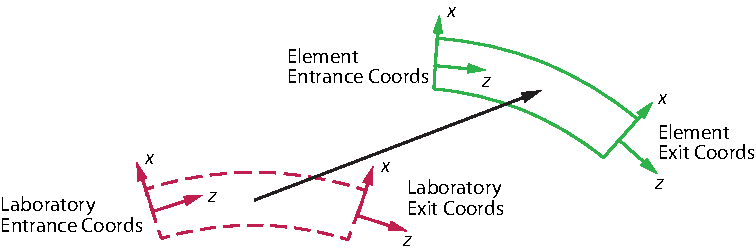
\includegraphics[width=5in]{coord-offset.pdf}
  \caption[Element Coordinate System.]
  {
\vn{Element} coordinates are coordinates attached to the physical element (solid green outline). The
\vn{laboratory} coordinates are fixed at the nominal position of the element (red dashed outline).
  }
  \label{f:ele.coord}.
\end{figure}

%-------------------------------------------------------------------------
\section{Hamiltonian}
\label{s:mag.hamiltonian}
The time dependent Hamiltonian $H_t$ in the curvilinear coordinate system shown
in \fig{f:local.coords} is (\cite{b:ruth})
\begin{equation}
  H_t = \wt\psi + \left[ \left( \frac{p_s - a_s}{1 + g\, x} \right)^2 + \wt m^2 + 
  (p_x - a_x)^2 + (p_y - a_y)^2 \right]^{1/2}
\end{equation}
where $(p_x, p_y, p_s/(1+gx))$ are the momentum normalized by $P_0$, $\rho$ being the local radius
of curvature of the reference particle, and $\wt m$, $\Bf a$ and $\wt\psi$ are the normalized mass,
vector, and scalar potentials:
\begin{equation}
  \wt m = \frac{m \, c^2}{c \, P_0} \qquad
  \left( a_x, a_y, \frac{a_s}{1+g \, x} \right) = \frac{q \, \Bf A}{P_0 \, c} \qquad 
  \wt\psi(x,y,z) = \frac{q \, \psi}{P_0}
  \label{mmccp}
\end{equation}
In terms of the normalized velocities $\beta_x$, $\beta_y$, the canonical momentum are
\begin{equation}
  p_x = \frac{m \, c^2}{P_0 \, c} \, \gamma \, \beta_x + a_x, \qquad 
  p_y = \frac{m \, c^2}{P_0 \, c} \, \gamma \, \beta_y + a_y
  \label{pmc2pc}
\end{equation}

The $s$-dependent Hamiltonian is obtained from $H_t$ by solving for
$-p_s$ and using a contact transformation to convert to \bmad
coordinates (\sref{s:phase.space}). For particles propagating in the
positive $s$ direction, the $s$-dependent Hamiltonian is, assuming
$\wt\psi$ is zero
\begin{equation}
  H \equiv H_s = -(1 + g \, x) \sqrt{(1 + p_z)^2 - (p_x - a_x)^2 - (p_y - a_y)^2} - 
  a_s + \frac{1}{\beta_0} \, \sqrt{(1+p_z)^2 + \wt m^2}
  \label{h1gx1}
\end{equation}
where $\beta_0$ is the reference velocity and the equality $(1 +
p_z)^2 = (E/c\, P_0)^2 - \wt m^2$ has been used. The last term on the
RHS of \Eq{h1gx1} accounts for the fact that the \bmad canonical $z$
(\Eq{zbctt}) has an ``extra'' term $\beta \, c \, t_0$ so that \bmad
canonical $z$ is with respect to the reference particle's $z$.

The equations of motion are
\begin{equation}
  \frac{dq_i}{ds} = \frac{\partial H}{\partial p_i} \qquad
  \frac{dp_i}{ds} = -\frac{\partial H}{\partial q_i}
  \label{rshp}
\end{equation}

\label{paraxial approximation} Without an electric field, $\psi$ is zero. Assuming a
non-curved coordinate system ($g = 0$), and using the paraxial approximation (which
expands the square root in the Hamiltonian assuming the transverse momenta are small)
(\sref{s:phase.space}), \Eq{h1gx1} becomes
\begin{equation}
  H = \frac{(p_x - a_x)^2}{2 (1 + p_z)} + \frac{(p_y - a_y)^2}{2 (1 + p_z)} - 
  (1 + p_z) - a_s +   \frac{1}{\beta_0} \, \sqrt{(1+p_z)^2 + \wt m^2}
  \label{hpapa}
\end{equation}

Once the transverse trajectory has been calculated, the longitudinal position
$z_2$ at the exit end of an element is obtained from symplectic
integration of \Eq{hpapa}
\begin{equation}
  z_2 = z_1 - \frac{1}{2 (1 + p_{z1})^2} \int \! ds \, 
  \left[ (p_x - a_x)^2 + (p_y - a_y)^2 \right] - \int \! ds \, g \, x
  \label{zz121p}
\end{equation}
where $z_1$ is the longitudinal position at the entrance end of the element.
Using the equations of motion \Eqs{rshp} this can also be rewritten as
\begin{equation}
  z_2 = z_1 - \frac{1}{2} \int \! ds \, 
  \left[ \left( \frac{dx}{ds} \right)^2 + \left( \frac{dy}{ds} \right)^2 \right] - 
  \int \! ds \, g \, x
  \label{zz12sx}
\end{equation}

For some elements, \vn{bmad_standard} uses a truncated Taylor map for
tracking.  For elements without electric fields where the particle
energy is a constant, the transfer map for a given coordinate $r_i$
may be expanded in a Taylor series
\begin{equation}
  r_{i,2} \rightarrow m_i + \sum_{j = 1}^4 m_{ij} \, r_{j,1} + 
  \sum_{j = 1}^4 \sum_{k = j}^4 m_{ijk} \, r_{j,1} \, r_{k,1} + \ldots
\end{equation}
where the map coefficients $m_{ij\cdots}$ are functions of $p_z$.  For
linear elements, the transfer map is linear for the transverse
coordinates and quadratic for $r_i = z$.

Assuming mid--plane symmetry of the magnetic field, so
that $a_x$ and $a_y$ can be set to zero\cite{b:madphysics}, The vector
potential up to second order is (cf.~\Eq{byx0b})
\begin{equation}
  a_s = -k_0 \left( x - \frac{g \, x^2}{2 (1 + g\, x)} \right) -
  \frac{1}{2} k_1 \left( x^2 - y^2 \right)
  \label{akxgx}
\end{equation}

For backwards propagation, where particle are traveling in the $-\Bf
s$ direction and where $p_s$ is negative, solving for $p_s$ involves
using a different part of the square root branch. There is also an
overall negative sign coming from switching from using $s$ as the
independent variable to $\wt s \equiv -s$ as the independent
variable. the Hamiltonian $H_{\wt s}$ is then
\begin{equation}
  H_{\wt s} = -(1 + g \, x) \sqrt{(1 + p_z)^2 - (p_x - a_x)^2 - (p_y - a_y)^2} + 
  a_s + \frac{1}{\beta_0} \, \sqrt{(1+p_z)^2 + \wt m^2}
\end{equation}

%---------------------------------------------------------------------------------
%---------------------------------------------------------------------------------
\section{Symplectic Integration}
\label{s:symp.track}
\index{symplectic integration}

Using \Eq{hpapa} the Hamiltonian is written in the form
\begin{equation}
  H = H_x + H_y + H_z
\end{equation}
where
\begin{equation}
  H_x = \frac{(p_x - a_x)^2}{2 (1 + \delta)}, \qquad
  H_y = \frac{(p_y - a_y)^2}{2 (1 + \delta)}, \qquad
  H_s = - a_s 
\end{equation}

For tracking, the element is broken up into a number of slices set by
the element's \vn{ds_step} attribute. For each slice, the tracking
uses a quadratic symplectic integrator $I$:
\begin{equation}
  I = T_{s/2} \; I_{x/2} \; I_{y/2} \; I_s \; I_{y/2} \; I_{x/2} \; T_{s/2}
\end{equation}
$T_{s/2}$ is just a translation of the $s$ variable:
\begin{equation}
  s \rightarrow s + \frac{ds}{2}
\end{equation}
And the other integrator components are
\begin{align}
  I_{x/2} &= \exp \left( : -\frac{ds}{2} H_x : \right) \CRNO
  I_{y/2} &= \exp \left( : -\frac{ds}{2} H_y : \right) \\
  I_{s}   &= \exp \left( : -ds \, H_s : \right) \nonumber
\end{align}
The evaluation of $I_{x/2}$ and $I_{y/2}$ is tricky since it involves both transverse
position and momentum variables. The trick is to split the integration into three parts.
For $I_{x/2}$ this is
\begin{align}
  I_{x/2} &= \exp \left( : -\frac{ds}{2} \frac{(p_x - A_x)^2}{2 (1 + \delta)} : \right) \CRNO
  &= \exp \left( : -\int A_x \, dx : \right) \,
     \exp \left( : -\frac{ds}{2} \frac{p_x^2}{2 (1 + \delta)} : \right) \,
     \exp \left( : \int A_x \, dx : \right)
  \label{ids2}
\end{align}
With an analogous expression for $I_{y/2}$.

\index{quadrupole}\index{sextupole}\index{wiggler}
For magnetic elements that do not have longitudinal fields
(quadrupoles, sextupoles, etc.), $a_x$ and $a_y$ can be taken to be
zero (cf.~\Eq{akxgx}).

\index{lcavity}\index{rfcavity}
For \vn{lcavity} and \vn{rfcavity} elements, the vector potential is computed from
\Eq{aiew}.

%---------------------------------------------------------------------------------
%---------------------------------------------------------------------------------
\section{BeamBeam Tracking}
\label{s:beambeam.std}
\index{beambeam}

A beam-beam element (\sref{s:beambeam}) simulates the effect on a tracked particle of an opposing
beam of particles moving in the opposite direction. The opposing beam, called the ``strong'' beam,
is assumed to be Gaussian in shape.

The strong beam is divided up into \vn{n_slice} equal charge (not equal thickness) slices.
Propagation through the strong beam involves a kick at the charge center of each slice with drifts
in between the kicks. The kicks are calculated using the standard Bassetti--Erskine complex error
function formula\cite{b:talman}.  Even though the strong beam can have a finite \vn{sig_z}, the
length of the element is always considered to be zero. This is achieved by adding drifts at either
end of any tracking so that the longitudinal starting point and ending point are identical. The
longitudinal $s$--position of the \vn{BeamBeam} element is at the center of the strong bunch. For
example, with \vn{n_slice} = 2 and with a solenoid field, the calculation would proceed as follows:
\begin{enumerate}[topsep=-0.2ex,itemsep=-0.0ex]
  \item 
Start with the particle longitudinally at the \vn{beambeam} element (which is considered to have
zero longitudinal length) in laboratory coordinates (\sref{s:coords.3}).
  %
  \item
Propagate backwards through the solenoid field so that the particle is in the plane of the first
beambeam slice. The fact that the plane of the slice may be, due to finite \vn{x_pitch} or
\vn{y_pitch} values, canted with respect to the laboratory $x$-$y$ plane is taken into account.
  %
  \item
Transform the particle coordinates to the \vn{beambeam} element body coordinates
(\sref{s:lab.body.transform}).
  %
  \item
Apply the beam--beam kick due to the first slice including a spin rotation.
  %
  \item
Transform back to laboratory coordinates.
  %
  \item
Propagate forwards so that the particle is in the plane of the second slice.
  %
  \item
Transform the particle coordinates to the \vn{beambeam} element body coordinates.
  %
  \item 
Apply the beam--beam kick due to the second slice.
  %
  \item 
Transform back to laboratory coordinates.
  %
  \item 
Propagate backwards through the solenoid field to end up with the particle longitudinally at the
\vn{beambeam} element.
  %
\end{enumerate}

There is an energy kick due to the motion of the strong beam. There are two parts to this $dp_z =
dp_{z,s} + dp_{z,h}$. One part, $dp_{z,s}$, is similar to the gravitational slingshot in orbital
mechanics. The slingshot energy kick is simply calculated using conservation of 4-momentum of the
tracked particle and the strong beam where the mass of the strong beam is assumed to be large
compared to the mass of the tracked particle.\footnote
  {
This assumption breaks down if a tracked particle is deflected due to a single scattering event with
a particle of the strong beam.  But particle-particle scattering is outside of the assumption of a
strong beam that is unaffected by the weak beam.
  }
After a little bit of algebra. The energy kick $dE_w$ to lowest order in the angle of the weak
particle with respect to the axis defined by the of motion of the strong beam is
\begin{equation}
  dE_w = \frac{c \, P_w}{2 \, (1/\beta_w + 1/\beta_s)} \, \left( \theta_{w2}^2 - \theta_{w1}^2 \right)
\end{equation}
where $P_w$ is the momentum of the weak particle, $\beta_w$ and $\beta_s$ are the weak and strong
beam velocities, and $\theta_{w1}$ and $\theta_{w2}$ are angles of the weak particle trajectory with
respect to the strong beam motion before and after the interaction. Converting to phase space
coordinates, the momentum kick $dp_z$ is
\begin{equation}
  dp_{z,s} = \frac{1}{2 \, \beta_w \, (1/\beta_w + 1/\beta_s) \, (1 + p_z)} 
    \left( dp_x \, (dp_x + 2p_{x1}) + dp_y \, (dp_y + 2p_{y1}) \right)
    \label{dpz12}
\end{equation}
where $dp_x$ and $dp_y$ are the transverse kicks and $p_{x1}$ and $p_{y1}$ are the initial phase
space momenta.

The other part of the energy kick, $dp_{z,h}$, happens when the strong beam's cross-section is changing due to
the hourglass effect. The hourglass longitudinal kick relative to the transverse kicks can derived using
Eq.~(5) of Sagan \cite{b:beamion}. In the relativistic limit the result is
\begin{equation}
  dp_{z,h} = \frac{\sigma_x}{2} \, \frac{d\sigma_x}{ds} \, \frac{dp_x}{dx} + 
             \frac{\sigma_y}{2} \, \frac{d\sigma_y}{ds} \, \frac{dp_y}{dy}
  \label{dpzsx}
\end{equation}
where $\sigma_x$ and $\sigma_y$ are the strong beam sizes, and the factor of two is due to the
relative velocity ($2c$) between the beams.

\newpage  % If newpage is removed, the footnote get put on the next page!!

%---------------------------------------------------------------------------------
%---------------------------------------------------------------------------------
\section{Bend: Exact Body Tracking with k1 = 0}
\label{s:bend.body.std}
\index{sbend}

\begin{figure}[h]
  \centering
  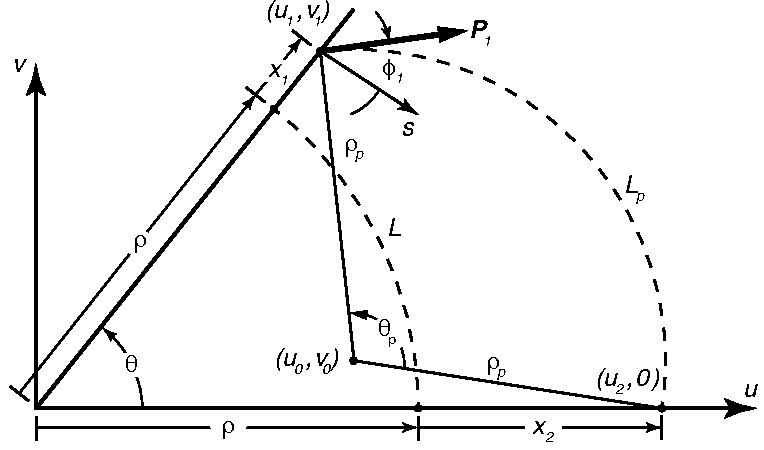
\includegraphics[width=5in]{bend-exact.pdf}
  \caption{Geometry for the exact bend calculation.}
  \label{f:bend.exact}
\end{figure}


Function definitions:
\begin{align}
  \sinc(x) &\equiv \frac{\sin(x)}{x} \\
  \cosc(x) &\equiv \frac{1 - \cos(x)}{x^2}
\end{align}
These functions cannot be directly evaluated at $x = 0$ and are defined at $x = 0$ using the $x
\rightarrow 0$ limit. The point to keep in mind here is that these functions are well behaved and
can be easily coded in software.

Referring to Figure~\ref{f:bend.exact}, at point 1 where the particle enters a sector bend, the angle
$\phi_1$ of the particle trajectory in the $(x,s)$ plane with respect to the $s$ axis is
\begin{equation}
  \sin(\phi_1) = \frac{p_{x1}}{\sqrt{(1+p_z)^2 - p_y^2}}
\end{equation}
where the subscript ``1'' for $p_z$ and $p_y$ is dropped since these quantities are invariant.

The $(u,v)$ coordinate system in the plane of the bend is defined with the $u$-axis along the exit
edge of the bend and the $v$-axis is perpendicular to the $u$-axis. The origin is at the design
center of the bend. In this coordinate system the point $(u_1, v_1)$ where the particle enters the
bend is given by
\begin{align}
  u_1 &= (\rho + x_1) \, \cos(\theta) \\
  v_1 &= (\rho + x_1) \, \sin(\theta)
\end{align}
where $\rho$ is the design radius of curvature, $x_1$ is the offset of the particle from the design
at the entrance point, and $\theta$ is the design bend angle
\begin{equation}
  \theta = \frac{L}{\rho} = g \, L
\end{equation}
with $L$ being the design arc length and $g \equiv 1/\rho$.

The coordinates $(u_0, v_0)$ of the center of curvature of the particle trajectory is
\begin{align}
  u_0 &= u_1 - \rho_p \, \cos(\theta + \phi_1) \\
  v_0 &= v_1 - \rho_p \, \sin(\theta + \phi_1)
\end{align}
where $\rho_p$ is the radius of curvature of the particle trajectory in the $(u, v)$ plane (see
\Eq{g1rg}).

The coordinates of the particle at the exit face is $(u_2, 0)$ where
\begin{equation}
  u_2 = u_0 + \sqrt{\rho_p^2 - v_0^2}
\end{equation}
After some manipulation, the offset of the particle $x_2$ from the design point at the exit face is
\begin{equation}
  x_2 = u_2 - \rho = x_1 \, \cos(\theta) - L^2 \, g \, \cosc(\theta) + \xi
\end{equation}
where $\xi$ can be expressed in two different ways
\begin{align}
  \xi &= \frac{\alpha}{\left[ \cos^2(\theta + \phi_1) + g_p \, \alpha \right]^{1/2} + \cos(\theta + \phi_1)} 
    \quad \text{or} \label{xctlg1} \\
  &= \frac{\left[ \cos^2(\theta + \phi_1) + g_p \, \alpha \right]^{1/2} - \cos(\theta + \phi_1)}{g_p}
    \label{xctlg2}
\end{align}
where
\begin{align}
  \alpha &= 2 \, (1 + g \, x_1) \, \sin(\theta + \phi_1) \, L \, \sinc(\theta) - 
        g_p \, (1 + g \, x_1)^2 \, L^2 \, \sinc^2(\theta) \\
  g_p &= \frac{1}{\rho_p} = \frac{g_\tot}{\sqrt{(1 + p_z)^2 - p_y^2}} \label{g1rg}
\end{align}
In the above equation $g_\tot$ is the bending strength of the actual field. Both \Eq{xctlg1} and
\Eq{xctlg2} are needed since \Eq{xctlg1} is singular when $\alpha = 0$ and $\theta + \phi_1 = \pi$
(which happens when the particle is bent by 180\Deg), and \Eq{xctlg2} is singular when $g_p$ is
zero. A simple way to implement the calculation for $x_2$ is to use \Eq{xctlg1} when $|\theta +
\phi_1| < \pi/2$ and otherwise use \Eq{xctlg2}.

Once $x_2$ is computed, the arc length of the particle $L_p$ is 
\begin{equation}
  L_p = \frac{|\bfL_c|}{\sinc(\theta_p/2)}
\end{equation}
where $\bfL_c$ is the vector (chord) from point 1 and point 2
\begin{equation}
  \bfL_c = (L_{cu}, L_{cv}) =
  \left( \xi, -L \, \sinc(\theta) - x_1 \, \sin(\theta) \right) 
\end{equation}
and $\theta_p$ is the angle made by the particle trajectory which is twice the angle between
the initial particle trajectory $\Bf P$ and the vector $\bfL_c$
\begin{equation}
  \theta_p = 2 \, \left( \theta + \phi_1 - \atantwo \left( L_{cu}, -L_{cv} \right) \right)
\end{equation}
where $\atantwo(y, x)$ is the standard two argument arctangent function.

Once $L_p$ is computed, $p_{x2}$, $y_2$ and $z_2$ are easily derived from
\begin{align}
  p_{x2} &= \sqrt{(1 + p_z)^2 - p_y^2} \, \sin(\theta + \phi_1 - \theta_p) \\
  y_2 &= y_1 + \frac{p_y \, L_p}{\sqrt{(1+p_z)^2 - p_y^2}} \\
  z_2 &= z_1 + \frac{\beta \, L}{\beta_\REF} - \frac{(1 + p_z) \, L_p}{\sqrt{(1+p_z)^2 - p_y^2}}
\end{align}
where $\beta$ is the normalized velocity of the particle and $\beta_\REF$ if the normalized
velocity of the reference particle.

Using the above equation, round-off error will give a non-zero final position even if the initial
position is zero. Even though the round-off error will be very small, a non-zero result can be
confusing. To avoid this, the standard linear transfer matrix for a bend is used if all the
following conditions are satisfied:
\begin{equation}
  |x \, g|, |p_x|, |p_y|, |p_z| <  10^{-9}, \quad \text{and}, \quad g_\tot = g
\end{equation}
The matrix is:
\begin{equation}
  \begin{pmatrix}
    \cos(\theta)            & L \, \sinc(\theta)  & 0 & 0 & 0 & g \, L^2 \, \cosc(\theta) \\
   -g \, \sin(\theta)       & \cos(\theta)        & 0 & 0 & 0 & g \, L \, \sinc(\theta)   \\
    0                       & 0                   & 1 & L & 0 & 0                         \\
    0                       & 0                   & 0 & 1 & 0 & 0                         \\
   -g \, L \, \sinc(\theta) & 
                       -g \, L^2 \, \cosc(\theta) & 0 & 0 & 1 & 
                   L \,  \left( \frac{1}{\gamma^2} - g^2 \, L^2 \, \sincc(\theta) \right) \\
    0                       & 0                   & 0 & 0 & 0 & 1                       
  \end{pmatrix}
\end{equation}
where
\begin{equation}
  \sincc(\theta) \equiv \frac{x - \sin(x)}{x^3}
\end{equation}

%---------------------------------------------------------------------------------
%---------------------------------------------------------------------------------
\section{Bend: Body Tracking with finite k1}
\label{s:bend.body.std.k1}
\index{sbend}

For a bend with a finite \vn{k1}, the Hamiltonian for the body of an \vn{sbend} is
\begin{equation}
  H = (g_\tot - g) \, x - g \, x \, p_z + 
  \frac{1}{2}\left( (k_1 + g \, g_\tot) x^2 - k_1 \, y^2 \right) +
  \frac{p_x^2 + p_y^2}{2 (1 + p_z)} 
\end{equation}

This is simply solved
\begin{align}
  x_2    &= c_x \, (x - x_c) + s_x \, \frac{p_{x1}}{1 + p_{z1}} + x_c \CRNO
  p_{x2} &= \tau_x \, \om_x^2 \, \, (1 + p_{z1}) \, s_x \, (x -x_c) + c_x \, p_{x1} \CRNO
  y_2    &= c_y \, y_1 + s_y \, \frac{p_{y1}}{1 + p_{z1}} \CRNO
  p_{y2} &= \tau_y \, \om_y^2 \, \, (1 + p_{z1}) \, s_y \, y_1 + c_y \, p_{y1} \\
  z_2    &= z_1 + m_5 + m_{51} (x - x_c) + m_{52} p_{x1} + m_{511} \, (x-x_c)^2 \, + \CRNO
         &\hspace*{20ex} m_{512} \, (x-x_c) \, p_{x1} + m_{522} \, p_{x1}^2 + 
                         m_{533} \, y^2 + m_{534} \, y_1 \, p_{y1} + m_{544} \, p_{y1}^2 \CRNO
  p_{z2} &= p_{z1} \nonumber
\end{align}
where 
\begin{alignat}{2}
  k_x &= k_1 + g \, g_\tot & \qqquad
  \om_x &\equiv \sqrt{\frac{|k_x|}{1 + p_{z1}}} \CRNO
  x_c &= \frac{g \, (1 + p_{z1}) - g_\tot}{k_x} & \qqquad
  \om_y &\equiv \sqrt{\frac{|k_1|}{1 + p_{z1}}} 
\end{alignat}
and
\begin{alignat}{6}
         &\hspace*{3ex}  && k_x > 0          &\hspace*{3ex}& k_x < 0 & \qqquad
         &\hspace*{3ex}  && k_1 > 0          &\hspace*{3ex}& k_1 < 0 \CRNO
     c_x &=   && \cos  (\om_x \, L)               && \cosh (\om_x \, L) & \qqquad
     c_y &=   && \cosh (\om_y \, L)               && \cos  (\om_y \, L) \CRNO
     s_x &=   && \frac{\sin  (\om_x \, L)}{\om_x} && \frac{\sinh (\om_x \, L)}{\om_x} & \qqquad
     s_y &=   && \frac{\sinh (\om_y \, L)}{\om_y} && \frac{\sin  (\om_y \, L)}{\om_y} \\
  \tau_x &=   && {-}1             && {+}1             & \qqquad
  \tau_y &=   && {+}1             && {-}1             \nonumber
\end{alignat}
and
\begin{alignat}{2}
  m_5     &= -g \, x_c \, L & \qqquad & \CRNO
  m_{51}  &= -g \, s_x & \qqquad
  m_{52}  &= \frac{\tau_x \, g}{1 + p_{z1}} \, \frac{1 - c_x}{\om_x^2} \CRNO
  m_{511} &= \frac{\tau_x \,\, \om_x^2}{4} \, (L - c_x \, s_x) & \qqquad
  m_{533} &= \frac{\tau_y \,\, \om_y^2}{4} \, (L - c_y \, s_y) \CRNO
  m_{512} &= \frac{-\tau_x \,\, \om_x^2}{2 \, (1 + p_{z1})} \, s_x^2 & \qqquad
  m_{534} &= \frac{-\tau_y \,\, \om_y^2}{2 \, (1 + p_{z1})} \, s_y^2 \CRNO
  m_{522} &= \frac{-1}{4 \, (1 + p_{z1})^2} \, (L + c_x \, s_x) & \qqquad
  m_{544} &= \frac{-1}{4 \, (1 + p_{z1})^2} \, (L + c_y \, s_y) \nonumber
\end{alignat}

%---------------------------------------------------------------------------------
%---------------------------------------------------------------------------------
\section{Bend: Fiducial Point Calculations}
\label{s:bend.fiducial}


When the \vn{fiducial_pt} switch for a bend is set to something other than \vn{none}, changing one
of \vn{rho}, \vn{g}, \vn{b_field} or \vn{angle} in a program (that is, changing after the lattice
has been read in and the bend parameters calculated) involves adjustment to the other three
parameters along with adjustment to \vn{e1}, \vn{e2}, \vn{l}, \vn{l_chord}, and
\vn{l_rectangle}. This is done to keep the shape of the bend invariant. Invariance is not maintained
with variation of any other parameter (EG variation of \vn{e1}).

\begin{figure}[tb]
  \centering
  \hfill
  \begin{subfigure}[b]{0.4\textwidth}
    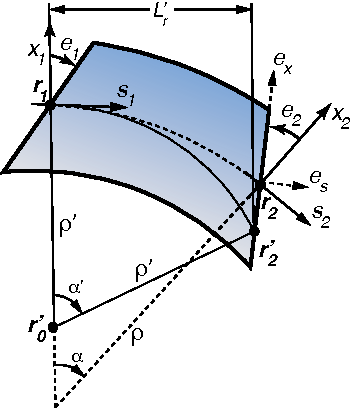
\includegraphics{bend-vary1.pdf}
    \caption{
With \vn{fiducial_pt} set to \vn{entrance_end}, $\bfr_1$ is the fiducial point at the entrance
end.  By construction, the entrance point $\bfr_1$ and the
slope of the reference curve at $\bfr_1$ is invariant with the reference curve before (dashed line)
and after (solid line) being tangent to $\bfs_1$ where $\bfs_1$ being the perpendicular to $\bfx_1$.
    }
    \label{f:bend.fid1}
  \end{subfigure}
  \hfill
  \begin{subfigure}[b]{0.4\textwidth}
    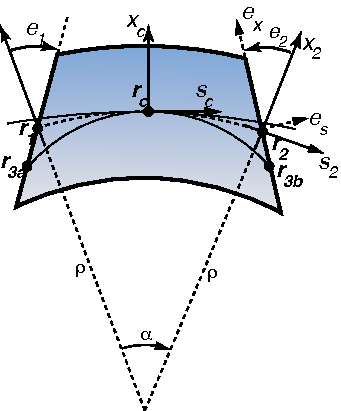
\includegraphics{bend-vary2.pdf}
    \caption{
With \vn{fiducial_pt} set to \vn{center}, $\bfr_c$ is the fiducial point at the center. By
construction, the reference curve always goes through $\bfr_c$ and the tangent of the reference
curve at $\bfr_c$ is invariant.}
    \label{f:bend.fid2}
  \end{subfigure}
  \hfill
  \caption{
Geometry with \vn{fiducial_pt} set to (a) \vn{entrance_end} and (b) \vn{center}. In both cases,
$\bfr_1$ and $\bfr_2$ are the entrance and exit reference points before and $\bfr'_1$ and $\bfr_2$
are the entrance and exit points after variation of one of \vn{rho}, \vn{g}, \vn{b_field}, or
\vn{angle}.  Similarly, $\rho$ and $\alpha$ are the bending radius and bending angle before
variation while $\rho'$ and $\alpha'$ are the bending radius afterwards.  Finally, $e_1$ $e_2$
are the face angles and rectangular length before variation, and $L'_r$ and $\bfr'_0$ are the
rectangular length and center of curvature after variation.
  }
  \label{f:bend.fid}
\end{figure}

\fig{f:bend.fid} shows the situation when the \vn{fiducial_pt} is set to either \vn{entrance_end} or
\vn{center} (the situation for the \vn{exit_end} setting is analogous to the \vn{entrance_end}
setting and so is not discussed). For any one of the \vn{fiducial_pt} settings discussed there are
essentially two cases. One case is direct variation of the bend field via variation of \vn{rho},
\vn{g}, or \vn{b_field}. This is called ``\vn{g}-variation''. The other type of variation is
variation of \vn{angle}. This is called ``angle-variation''. The discussion below shows how, with
\vn{g}-variation, \vn{l}, \vn{e1}, and \vn{e2} are calculated. With \vn{angle}-variation, \vn{l},
\vn{g}, \vn{e1}, and \vn{e2} need to be calculated. Once \vn{l} and \vn{g} are know, the other
parameters \vn{l_chord}, \vn{l_rectangle}, \vn{l_sagitta} (and \vn{angle} for the \vn{g}-variation
case) can be readily computed.

The \vn{entrance_end} analysis is as follows (\fig{f:bend.fid1}). The entrance end coordinates
around the point $\bfr_1$ are held fixed and as as a result $\bfr'_1 = \bfr_1$ and \vn{e1} does not
vary as well. $\bfr_2$ is the exit point before variation and $\bfr_3$ is the exit point after. The
position of $\bfr_3$ is calculated by first calculating the position of $\bfr_1$ in a coordinate
system centered at $\bfr_2$ and with axes parallel to the $(\bfs_1, \bfx_1)$ axes of the coordinate
system at $\bfr_1$
\begin{equation}
  \bar\bfr_1 = \left( -l_{\text{rectangle}}, \rho \, (1 - \cos\alpha) \right)
\end{equation}
Where the bar denotes that the coordinates are in the $(\bfs_1, \bfx_1)$ system.
The coordinates of $\bfr_1$ in the $(\bfe_s, \bfe_x)$ coordinate system
with origin at $\bfr_2$ and with $\bfe_x$ along the bend edge and $\bfe_s$ perpendicular to $\bfe_x$
is a rotation $\bfR(\theta)$ 
\begin{equation}
  \bfr_1 = \bfR(\alpha - e_2) \, \bar\bfr_1
\end{equation}
The angle $\theta_1$ of the vector $\bfs_1$, which is the invariant tangent of the reference curve
at the point $\bfr_1$, in the $(\bfe_s, \bfe_x)$ coordinate system (which is used from here on) is
\begin{equation}
  \theta_1 = \alpha - e_1
\end{equation}
The center of curvature after variation $\bfr'_0$ is 
\begin{equation}
  \bfr'_0 = \bfr_1 + \rho' \, \left( \sin\theta_1, -\cos\theta_1 \right)
\end{equation}
The reference trajectory after variation $\bfr'$ is a circular arc subject to the condition
\begin{equation}
  \left| \bfr' - \bfr'_0 \right| = \rho'^2
  \label{rr0r}
\end{equation}
With \vn{g}-variation, the value of $\rho'$ is set (perhaps indirectly) by the User. To find the
point $\bfr'_2$, it is noted that in the $(e_s, e_x)$ coordinate system,  the $s$
coordinate of $\bfr'_2$, $r'_{2s}$ is zero.
so using this in\Eq{rr0r} and throwing away the unphysical root gives for the $x$ coordinate
\begin{equation}
  r'_{2x} = r_{1x} + \frac{2 \, c}{-b - \sqrt{b^2-4 \, a \, c}}
\end{equation}
where
\begin{align}
  a &= g' \CRNO
  b &= 2 \, \cos\theta_1 \\
  c &= g' \, r_{1s}^2 + 2 \, r_{1s} \, \sin\theta_1 \nonumber
\end{align}
where $g' = 1 / \rho'$.
The rectangular length after variation $L'_r$ is then
\begin{equation}
  L'_r = L_r + r'_{2x} * \sin\theta_1
\end{equation}
where $L_r$ is the rectangular length before variation.
Finally, the length $L'$ after variation is
\begin{equation}
  L' = \text{asinc} \left( g' \, L'_r \right) \, L'_r
\end{equation}
where $\text{asinc}$ is the function
\begin{equation}
  \text{asinc}(\theta) = \frac{\sin^{-1}(\theta)}{\theta}
\end{equation}

For \vn{fiducial_pt} set to \vn{entrance_end} and with \vn{angle}-variation, $\alpha'$ is know and
$g'$ can be computed via
\begin{equation}
  g' = \frac{\sin(\alpha' - \theta_1) + \sin(\theta_1)}{r_{1s}}
  \label{gatt}
\end{equation}
With this, all other parameters can be created. In both \vn{angle}-variation and \vn{g}-variation the new
face angle $e'_2$ is given by
\begin{equation}
  e'_2 = e_2 + \alpha' - \alpha
\end{equation}

For \vn{fiducial_pt} set to \vn{center}, The center point $\bfr_c$ (see \fig{f:bend.fid2}) is held
constant.  Here the \vn{g}-variation analysis is similar to the \vn{g}-variation analysis with
\vn{fiducial_pt} set to \vn{entrance_end} (or \vn{exit_end} except in this case the reference orbit
to the right and left of $bfr_c$ are analyzed separately and the two lengths for each piece are
added together. For \vn{angle}-variation, the only situation where it is possible to keep $\bfr_c$
fixed while varying the angle is when \vn{e1} and \vn{e2} are equal. In this instance, the
calculation is again similar to the \vn{angle}-variation analysis with the \vn{fiducial_pt} set to
either end. If \vn{e1} and \vn{e2} are not equal, a calculation is done that gives the desired angle
but the center point will shift.

%---------------------------------------------------------------------------------
%---------------------------------------------------------------------------------
\section{Converter Tracking}
\label{s:converter.track}
\index{converter} 

Tracking through a \vn{converter} element involves generating five random numbers
  \footnote{
Since the outgoing particle starts at the exit surface of the converter only five numbers
are needed to generate the 6-dimensional particle phase space position.
  }
and then using these numbers with the outgoing particle distribution to generate the position and
orientation of the outgoing particle. The outgoing particle distribution is pre-computed by a
program \vn{converter_element_modeling} and the distribution parameters are included in the
converter element description in the \bmad lattice file (\sref{s:converter}). The accuracy of the
converter modeling will depend in part upon the granularity of the probability tables generated
by the \vn{converter_element_modeling} program and on other approximations made during
tracking. Generally, inaccuracies in the 1\% to 10\% range are to be expected.

In a tracking simulation, a single outgoing particle is generated for each incoming particle. Since,
in a real machine, the number of outgoing particles will not be equal to the number of incoming
particles, each outgoing particle is assigned a weight such that the weighted distribution of
outgoing particles is correct. This weight will be the same for all outgoing particles. The weight
will depend upon whether the momentum or angular range of the outgoing particles is restricted using
the element parameters (\sref{s:converter}):
\begin{example}
  pc_out_min    ! Minimum momentum of generated outgoing particles (eV).
  pc_out_max    ! Maximum momentum of generated outgoing particles (eV).
  angle_out_max ! Maximum angle to the surface perpendicular (rad).
\end{example}

%-------------------------------------------------------------------------

\begin{figure}[tb]
  \centering
  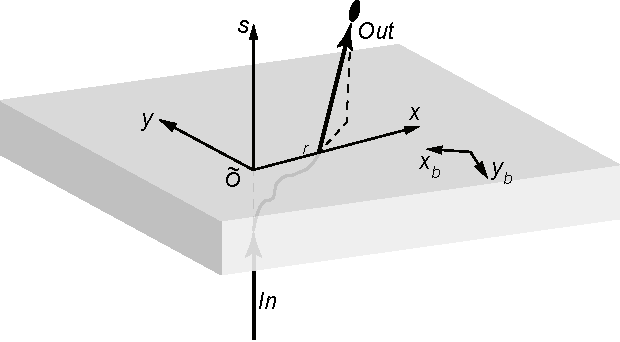
\includegraphics[width=5in]{converter.pdf}
  \caption[Converter geometry.]
  {
An incoming particle strikes the bottom of the converter. At some point within the interior, a new
particle is generated and this new particle exits the top surface. To calculate the position and
orientation of the outgoing particle, a coordinate system is established where the origin point
$\wt\calO$ is the point that the incoming particle would strike the top surface if it went straight
through and the $(x,y)$ axes are randomly rotated with respect to the $(x_b,y_b)$ body coordinate axes.
By construction, the position of the outgoing particle will be along the $x$-axis.
  }
  \label{f:converter}.
\end{figure}

%-------------------------------------------------------------------------

The geometry of the converter is shown in \fig{f:converter}. On the top surface, where the outgoing
particle emerges, $(x_b,y_b)$ are the axes for the element body coordinate system (\sref{s:coords.3}).
To generate the position and orientation of the outgoing particle, another coordinate system is used
with axes labeled by $(x,y)$. Each outgoing particle will be assigned its own $(x,y)$
axes. The origin $\wt\calO$ of this coordinate system is constructed by placing $\wt\calO$ at the
point where the incoming particle under consideration would strike the top surface if the incoming
particle would pass straight through the converter. The angular orientation of the $(x,y)$ axes
with respect to the $(x,y)$ axes is chosen using a random number with a uniform probability
distribution in the interval $[0, \pi]$. By construction, the outgoing particle, at the surface of
the converter will be generated at a point a distance $r$ along the $x$-axis.

The particle distribution is calculated at a number of converter thickness $t_i$, $i = 1 \ldots
N_t$. It is an error if the actual converter thickness is outside the range of these
thicknesses. [The exception is if only one distribution for a given thickness is present, this
distribution is used to generate the outgoing particle coordinates independent of the converter
thickness.]  The particle distribution is also calculated within a certain incoming particle
momentum range. It is also an error if an incoming particle has a momentum outside of this range.

The first step is to choose the value of the outgoing particle's momentum $p_\txt{out}$. For each
thickness $t_i$, the pre-computed particle distribution parameters includes a two-dimensional table
of $P(p_\txt{out}, r)$ --- the probability density of creating an outgoing particle versus
$p_\txt{out}$ and $r$. $P(p_\txt{out},r)$ is normalized so that the integrated probability is equal
to the average number of outgoing particles created for each incoming particle $N_\txt{out}/N_{in}$
\begin{equation}
  \frac{N_\txt{out}}{N_{in}} = \int \int dp_\txt{out} \, dr \, P(p_\txt{out}, r)
  \label{nnprp}
\end{equation}
The integrals are done using linear interpolation between grid points.  From a $P(p_\txt{out},r)$
probability table, a ``normalized'' probability $P_\txt{n}(p_\txt{out},r)$ table is computed where
$P_\txt{n}$ is the probability of generating a particle at given $p_\txt{out}$ and $r$ with an
angular range restricted by \vn{angle_out_max}. If \vn{angle_out_max} is not set, $P_\txt{n}$ will
be equal to $P$.  This calculation is part of a ``setup'' computation done before tracking which, to
save time, is only done if one of the three element parameters, \vn{pc_out_min}, \vn{pc_out_max}, or
\vn{angle_out_max}, changes. Additionally, the setup includes creating a table of $I(p_\txt{out})$
which is the integrated probability for generating a particle with momentum less than $p_\txt{out}$
\begin{equation}
  I_p(p_\txt{out}) = \frac{\dstyle \int_{p_\txt{min}}^{p_\txt{out}} d\pw_\txt{out} 
  \int dr \, P_\txt{n}(\pw_\txt{out}, r)}
  {\dstyle \int_{p_\txt{min}}^{p_\txt{max}} d\pw_\txt{out} \int dr \, P_{n}(\pw_\txt{out}, r)}
\end{equation}
where $p_\txt{min}$ is the minimum momentum in the $P(p_\txt{out}, r)$ table or the value of
\vn{pc_out_min} which ever is greatest and $p_\txt{max}$ is the maximum momentum in the
$P(p_\txt{out}, r)$ table or the value of \vn{pc_out_max} which ever is smallest. $I(p_\txt{out})$
is normalized such that $I(p_\txt{max}) = 1$. A value for $p_\txt{out}$ is generated by solving
numerically for $p_\txt{out}$ the equation
\begin{equation}
  I_p(p_\txt{out}) = R_1
\end{equation}
where $R_1$ is a random number with uniform distribution in the interval $[0,1]$.  This
calculation is done for the two $t_i$ thicknesses that straddle the actual thickness. The value of
$p_\txt{out}$ assigned to the outgoing particle is obtained via linear interpolation between the two
computed values. Note that for both thicknesses the same random number needs to be used.

The next step is to choose a value for $r$. This is done by solving the equation
\begin{equation}
  I_r(r) = R_2
\end{equation}
where $R_2$ is another random number with uniform distribution in the interval $[0,1]$ and $I_r$ is 
\begin{equation}
  I_r(r) = \frac{\dstyle \int_0^r d\rw \, P_\txt{n}(p_\txt{out}, \rw)}
  {\dstyle \int_0^{r_\txt{max}} d\rw \, P_{n}(p_\txt{out}, \rw)}
\end{equation}
with $p_\txt{out}$ being the momentum chosen for the particle and $r_\txt{max}$ being the maximum
radius the probability table goes out to\footnote
  {
The range $[0,r_\txt{max}]$ encompasses nearly all of the outgoing particles. In principle, the
integral could be extended by extrapolating the values in the table but this could potentially lead
to inaccuracies in determining the outgoing orientation. Generally the inaccuracy in truncating the
distribution at $r_\txt{max}$ should be small.
  }. 
Like $p_\txt{out}$, this calculation is done for the two
$t_i$ thicknesses that straddle the actual thickness. The value of $r$ assigned to the outgoing
particle is obtained via linear interpolation between the two computed values. Note that for both
thicknesses the same random number needs to be used.

Once $p_\txt{out}$ and $r$ have been chosen, the next steps are to choose values for the angular
orientation of the outgoing particle. The angular orientation is characterized by the distribution
parameters using the derivatives $x' = dx/ds$ and $y' = dy/ds$ in the form of a skewed Lorentzian
probability distribution $P_d$
\begin{equation}
  P_d\left( x', y' ; p_\txt{out}, r \right) =
  A_d \, \frac{1 + \beta \, x'}{1 + \alpha_x^2 \, \left( x' - c_x \right)^2 +
  \alpha_y^2 \, \left( y' \right)^2}
  \label{pxsxs}
\end{equation}
where the parameters $A_d$, $\beta$, $c_x$, $\alpha_x$, and $\alpha_y$ all depend upon $p_\txt{out}$
and $r$. Notice that by construction, with the outgoing particle generated on the $x$-axis, the
distribution is symmetric about $y'$-axis. The pre-computed distribution characterizes each of these
parameters by a set of one or more fits which are functions of $p_\txt{out}$ and $r$. There are also
four functions of $p_\txt{out}$ and $r$ that give the range over which \Eq{pxsxs} is valid
$x'_\txt{min}$, $x'_\txt{max}$, $y'_\txt{min}$, and $y'_\txt{max}$. By symmetry, $y'_\txt{min} =
-y'_\txt{max}$. Also $A_d$ can be computed from knowledge of $\beta$, $c_x$, $\alpha_x$, and
$\alpha_y$ using the normalization condition that at any given $p_\txt{out}$ and $r$
\begin{equation}
  1 = \int_{x'_\txt{min}}^{x'_\txt{max}} dx' 
  \int_{-y'_\txt{max}}^{y'_\txt{max}} dy' \, P_d \left( x', y' \right)
\end{equation}
Thus there are only seven independent parameters that need to be fitted. The fit functions for all
seven have the same form. The fit is divided into two regions. For $p_\txt{out}$ lower than some
cutoff, a parameter is fit using a set of one-dimensional functions $\Gamma_i(r)$ at discrete momentum $p_i$,
$i = 1, \ldots, N_\beta$ with
\begin{equation}
  \Gamma_i(r) = \sum_{n=1}^M c_{n,i} \, r^n
  \label{gcr}
\end{equation}
The polynomial cutoff $M$ is 4 for $c_x$ and $\beta$ and is 3 for the other five.  To evaluate a
parameter at momenta lower than $p_{N_\beta}$, the $\Gamma_i$ are used with linear interpolation in
$p$ between functions of different $p_i$. At higher energies, the parameter variation is smoother so
a two dimensional fit $Xi$ is used
\begin{equation}
  \Xi(p_\txt{out},r) = e^{-(k_p \, p_\txt{out} + k_r \, r)} \,
  \left( \sum_{n=0}^3 k_{n} \, r^n \right) \, 
  \left( 1 + \sum_{n=1}^3 w_{n} \, p_\txt{out}^n \right) + C
  \label{xkpkr}
\end{equation}
The $C$ parameter is only nonzero for $x'_\txt{min}$. 

Once $A_d$, $\beta$, $c_x$, $\alpha_x$, and $\alpha_y$ have been calculated for a given $p_\txt{out}$ and
$r$, The calculation of $x'$ starts with integrating $P_d$ in \Eq{pxsxs} over $y'$
\begin{align} 
  I_{xd} (x') &\equiv \int_{-y'_\txt{lim}}^{y'_\txt{lim}} dy' \, P_d(x', y')
  \label{ixdyp} \\
  &= 2 \, A_d \, \frac{1 + \beta \, x'}{\alpha_y \, \sqrt{1 + \alpha_x^2 \, (x' - c_x)^2 }} \,
  \tan^{-1} \left( \frac{\alpha_y \, y'_\txt{lim}}{\sqrt{1 + \alpha_x^2 \, (x' - c_x)^2}} \right)
  \nonumber
\end{align}
where $y'_\txt{lim}$ is either the lesser of $y'_\txt{max}$ and $\tan^{-1}(\text{angle_out_max})$.
A spline fit is used to integrate $I_{xd}$ and this is used to choose a value for $x'$. Once $x'$
is known, The integral of $P_d(x', y')$ over $y'$ is used to choose a value for $y'$.

Except for the placement of $\wt\calO$, the above algorithm for calculating the position and
orientation of the outgoing particle will be independent of the angular orientation of the incoming
particle. This is valid for incoming particles that are traveling perpendicular to the converter
surface. To the extent that the incoming particles are not perpendicular to the converter, this will
introduce inaccuracies. Typically, however, the incoming particles will be fairly close to being
perpendicular. Considering this, and considering the approximations used to calculate the
distribution parameters, the neglect of incoming particle orientation effects is usually justified.

%---------------------------------------------------------------------------------
%---------------------------------------------------------------------------------
\section{Drift Tracking}
\label{s:drift.std}
\index{drift} 

\bmad uses the exact map for a drift
This gives the map
\begin{align}
  x_2    &= x_1 + \frac{L \, p_{x1}}{p_l} \CRNO
  p_{x2} &= p_{x1}  \CRNO
  y_2    &= y_1 + \frac{L \, p_{y1}}{p_l} \CRNO
  p_{y2} &= p_{y1}  \\
  z_2    &= z_1 + \left( \frac{\beta}{\beta_\REF} - \frac{1 + p_{z1}}{p_l} \right) \, L \CRNO
  p_{z2} &= p_{z1} \nonumber
\end{align}
where $\beta$ is the normalized particle velocity, $\beta_\REF$ is the reference particle's
normalized velocity, and $p_l$ is the normalized longitudinal momentum 
\begin{equation}
  p_l \equiv \frac{P_l}{P_0} = \sqrt{(1 + p_z)^2 - p_x^2 - p_y^2}
\end{equation}
with $P_l$ being the longitudinal momentum.

%---------------------------------------------------------------------------------
%---------------------------------------------------------------------------------
\section{ElSeparator Tracking}
\label{s:elsep.std}
\index{elseparator}

\begin{figure}[tb]
  \centering
  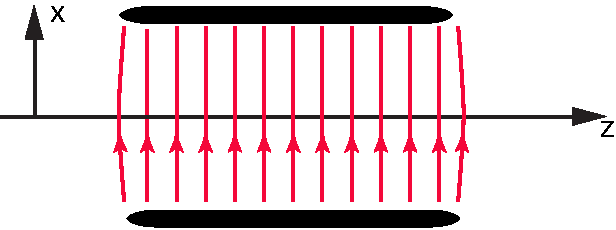
\includegraphics[width=5in]{elseparator.pdf}
  \caption[ElSeparator electric field.]
  {
Elseparator Electric field. The fringe field lines break the
translational invariance in $x$.
  }
  \label{f:elsep}.
\end{figure}

[Thanks to \'Etienne Forest for the derivation of the elseparator equation of motion.]

The Hamiltonian for an electric separator is 
\begin{equation}
  H = -p_s 
  = - \left\{ \left( \frac{1}{\beta_0} + \delta + k_E \, x \right)^2 - 
  \wt m^2 - p_x^2 - p_y^2 \right\}^{1/2}
  \label{hp1b}
\end{equation}
Here the canonical coordinates $(-c \, t, \delta$ are being used, $\wt m$ is defined in \Eq{mmccp},
and $p_s = -H$ is just the longitudinal momentum.  In the above equation, $k_E$ is the normalized
field
\begin{equation}
  k_E = \frac{q \, E}{P_0 \, c}
\end{equation}
The field is taken to be pointing along the $x$-axis with positive $k_E$ accelerating a particle in
the positive $x$ direction. To solve the equations of motion, a ``hard edge'' model is used where
$k_E$ is constant inside the separator and the field ends abruptly at the separator edges.

\index{solenoid}
Since, as shown in \fig{f:elsep}, the fringe fields break the translational invariance in $x$, it is
important here that the $x = 0$ plane be centered within the separator plates. With this, the
canonical momentum $\delta$ just outside the separator assumes its free space form of $\delta = (E -
E_0) / E_0)$. This is analogous to the case of a \vn{solenoid} where, to ensure that the canonical
transverse momenta assume their free space form just outside the solenoid, the $\Bf z$-axis must be
along the centerline of the solenoid.

The solution of the equations of motion is:
\begin{align}
  x   &= (x_0 - x_c) \, \cosh \left( \frac{k_E \, L}{p_s} \right) + 
         \frac{p_{x0}}{k_E} \, \sinh \left( \frac{k_E \, L}{p_s} \right) + x_c \CRNO
  p_x &= k_E \, (x_0 - x_c) \, \sinh \left( \frac{k_E \, L}{p_s} \right) + 
         {p_{x0}} \, \cosh \left( \frac{k_E \, L}{p_s} \right) \CRNO
  y   &= y_0 + L \, \frac{p_{y0}}{p_s} \label{xxlp} \\
  p_y &= p_{y0} \CRNO
  c \, \delta t &=  \int_0^L -\frac{\partial H}{\partial \delta}
      = (x_0 - x_c) \, \sinh \left( \frac{k_E \, L}{p_s} \right) +
        \frac{p_{x0}}{k_E} \, \left[ \cosh \left( \frac{k_E \, L}{p_s} \right) - 1 \right]
        \nonumber
\end{align}
where the critical position $x_c$ is
\begin{equation} 
  x_c = -\frac{\wt E}{k_E}
\end{equation}
and 
\begin{equation}
  \wt E \equiv \frac{1}{\beta_0} + \delta = \frac{E}{P_0 \, c}
\end{equation}
 
\Eqs{xxlp} predict that for $x < x_c$ and $p_{x0} = 0$ a particle will, unphysically, accelerate in
the negative $x$ direction. In actuality, a particle in this instance will be reflected backwards by
the longitudinal component of the edge field. Specifically, the argument of the square root in
\Eq{hp1b} must be non-negative and a particle will only make it through the separator if
\begin{equation}
  x_0 > \frac{1}{k_E} \, \left( \sqrt{\wt m^2 + p_{x0}^2 + p_{y0}^2} - \wt E \right)
\end{equation}

%---------------------------------------------------------------------------------
%---------------------------------------------------------------------------------
\section{Foil Tracking}
\label{s:foil.std}
\index{foil}

A particle going through a \vn{foil} element is scattered both in angle and in energy, and the
charge of the particle may be affected. The following two subsections give the formulas used for
scattering and energy loss. Currently, the final charge is a fixed number but that may change in the
future.

%---------------------------------------------------------------------------------
\subsection{Scattering in a Foil}
\label{s:foil.scatter}

For the angle scattering, the user can select between one of two algorithms, both
of which are given in the paper by Peralta and Louro\cite{b:peralta} (also see Lynch and Dahl\cite{b:lynch})
Both methods vary the phase space $p_x$ and $p_y$ coordinates using:
\begin{equation}
  (dp_x, dp_y) = \frac{p \, \sigma}{P_0} \, (r_1, r_2)
  \label{dpr1s}
\end{equation}
where $p$ is the
particle momentum, $P_0$ is the reference momentum, $r_1$ and $r_2$ are Gaussian random numbers with
unit sigma and zero mean, and $\sigma$ is the sigma of the angular scattering distribution. The
factor of $p/P_0$ is due to a translation between change in angle and change in phase space momenta
(see \Eq{xpa1p}). 

The \vn{Highland} algorithm uses Eq.~(32) of Peralta and Louro\cite{b:peralta} to calculate the
scattering sigma:
\begin{equation}
  \sigma = \frac{(13.6 \cdot 10^6~eV) \, z}{p \, c \, \beta} \sqrt{\frac{X}{X_0}} \, \left[
  1 + 0.038 \, \ln \left( \frac{X \, z^2}{X_0 \, \beta^2} \right) \right]
  \label{sszpb}
\end{equation}
where $X_0$ is the material radiation ``length'' in kg/m$^2$, $z$ is the particle charge, $\beta$ is the particle
relativistic beta, $c$ is the speed of light, and $X$ is the foil area density in kg/m$^2$ equal
to $\rho \, t$ where $\rho$ is the material density and $t$ is the foil thickness.

The \vn{Lynch_Dahl} algorithm uses Eq.~(33) of Peralta and Louro:
\begin{equation}
  \sigma^2 = \frac{\chi_c^2}{1 + F^2} \left[ \frac{1 + \nu}{\nu} \ln (1 + \nu) - 1 \right]
  \label{sc1f}
\end{equation}
where
\begin{align}
  \nu &= \frac{0.5 \, \Omega}{(1 - F)} \CRNO
  \Omega &= \frac{\chi_c^2}{1.167 \, \chi_\alpha^2} \CRNO
  \chi_c^2 &= \left( 1.57 \cdot 10^{10} \, \frac{eV^2 \, m^2}{kg} \right) \, 
    \frac{Z (Z+1) X}{A} \left[ \frac{z}{p \, \beta} \right]^2 
  \label{no1f} \\
  \chi_\alpha &= (2.007 \cdot 10^7 \, eV^2) \, \frac{Z^{2/3}}{(p \, c)^2} 
            \left[1 + 3.34 \,  \left( \frac{Z \, z \, \alpha}{\beta} \right)^2 \right] \nonumber
\end{align}
and the $A$ is the atomic weight, $p$ is the particle momentum, $\alpha$ is the fine structure
constant, and $F$ is a fit parameter representing the percent of the central angular distribution
that is used.  $F$ is a settable parameter with a default value of 0.98.

For compound materials, the value of $X/X_0$ in \Eq{sszpb} is computed from
\begin{equation}
  \frac{X}{X_0} = \sum_{i = 1}^N \frac{X_i}{X_{0i}}
\end{equation}
where the summation is over all constituents in the material.

Also for compound materials, $\chi_c^2$ in \Eqs{sc1f} and \eq{no1f} is replaced by the sum of the
constituent $\chi_{ci}^2$, and $\chi_\alpha$ is computed from Lynch and Dahl Eq.~(11)
\begin{equation}
  \ln ( \chi_\alpha ) = \left. \sum_{i=1}^N \frac{Z_i (Z_i + 1) X_i}{A_i} \ln(\chi_{\alpha i}) \middle/
  \sum_{i=1}^N \frac{Z_i (Z_i + 1) X_i}{A_i} \right.
\end{equation}

The actual scattering distribution has $1/\theta^4$ tails ($\theta$ is the scattering angle) due to
single event large angle scattering (Rutherford scattering). By assuming a Gaussian distribution,
these tails are not present in a simulation. It is also important to note that with both the
\vn{Highland} and \vn{Lynch_Dahl} algorithms, simulating the passage of particles through a single
foil versus two foils with half the thickness as the single foil will not give exactly the same
results. This is just a reflection that both algorithms are trying to model an inherently non-Gaussian
process.

%---------------------------------------------------------------------------------
\subsection{Energy Loss in a Foil}
\label{s:foil.eloss}

The particle energy loss per unit length $dE/dx$ through a foil is calculated using the \vn{Bethe-Bloch} formula
\begin{equation}
  - \left\langle\frac{dE}{dx}\right\rangle = 
  \frac{4 \pi}{m_e c^2} \cdot \frac{nz^2}{\beta^2} \cdot \left(\frac{e^2}{4\pi\varepsilon_0}\right)^2 \cdot 
  \left[\ln \left(\frac{2m_e c^2 \beta^2}{I \cdot (1-\beta^2)}\right) - \beta^2\right]
  \label{ex4pmc}
\end{equation}
where $n$ is the material electron density, $I$ is the mean excitation energy, $z$ is the particle
charge, $c$ is the speed of light, $\epsilon_0$ is the vacuum permittivity, $\beta = {v}/{c}$, is
the normalized velocity, and $e$ and $m_e$ the electron charge and rest mass respectively.

Note that to keep the direction of travel of the particle constant when energy is lost, this implies
that $p_x/(1+p_z)$ and $p_y/(1+p_z)$ are to be held constant (\Eq{xpa1p}).

%---------------------------------------------------------------------------------
%---------------------------------------------------------------------------------
\section{Kicker, Hkicker, and Vkicker Tracking}
\label{s:kicker.std}
\index{kicker}
\index{hkicker}
\index{vkicker}
\index{elseparator}

The Hamiltonian for a horizontally deflecting kicker or separator is
\begin{equation}
  H = \frac{p_x^2 + p_y^2}{2 (1 + p_z)} - k_0 \, x 
\end{equation}
This gives the map
\begin{alignat}{2}
  x_2 &= x_1 + \frac{1}{1 + p_{z1}} \, \left( L \, p_{x1} + \frac{1}{2} k_0 \, L^2 \right), &
    p_{x2} &= p_{x1} + k_0 \, L, \CRNO
  y_2 &= y_1 + \frac{L \, p_{y1}}{1 + p_{z1}}, &
    p_{y2} &= p_{y1},  \\
  z_2 &= z_1 - \frac{L}{2 (1 + p_{z1})^2} \, 
    \left( p_{x1}^2 + p_{y1}^2 + p_{x1} \, k_0 \, L + \frac{1}{3} k_0^2 \, L^2 \right), \quad &
  p_{z2} &= p_{z1} \nonumber
\end{alignat}
The generalization when the kick is not in the horizontal plane is easily derived.

%---------------------------------------------------------------------------------
%---------------------------------------------------------------------------------
\section{LCavity Tracking}
\label{s:lcavity.std}
\index{lcavity}

For tracking using something like \vn{runge_kutta}, with \vn{field_calc} set to \vn{bmad_standard},
the fields are modeled by the equations given in Sections~\sref{s:rf.fields} and \sref{s:rf.fringe}.

For \vn{bmad_standard} tracking, and with \vn{cavity_type} set to \vn{standing_wave}, the transverse
trajectory through an \vn{Lcavity} is modeled using equations developed by Rosenzweig and
Serafini\cite{b:rosenzweig} (R\&S) with
\begin{equation}
  b_0 = 1, \qquad \text{and} \qquad b_{-1} = 1 
\end{equation}
and all other $b_n$ set to zero.

The transport equations in R\&S were developed in the ultra-relativistic limit with $\beta = 1$.  To
extend these equations to lower energies, the transport through the cavity body (R\&S Eq.~(9)) has
been modified to give the correct phase-space area at non ultra-relativistic energies:
\begin{equation}
  \begin{pmatrix}
    x \\ 
    x'
  \end{pmatrix}_2 = \sqrt{\frac{\beta_1}{\beta_2}} \, 
  \begin{pmatrix}
    \cos(\alpha)  &
        \sqrt{\frac{8}{\eta(\Delta\phi)}} \, \frac{\, \gamma_1}{\gamma'} \, \cos(\Delta\phi) \, \sin(\alpha) \\
    -\sqrt{\frac{\eta(\Delta\phi)}{8}} \, \frac{\gamma'}{\gamma_2 \, \cos(\Delta\phi)} \, \sin(\alpha) &
        \frac{\gamma_1}{\gamma_2} \, \cos(\alpha)
  \end{pmatrix}
  \,
  \begin{pmatrix}
    x \\ 
    x'
  \end{pmatrix}_1
  \label{xxpc}
\end{equation}
The added factor of $\sqrt{\beta_1/\beta_2}$ gives the matrix the correct determinant of $\beta_1 \,
\gamma_1 / \beta_2 \, \gamma_2$. {\em While the added factor of $\sqrt{\beta_1/\beta_2}$ does
correct the phase space area, the above equation can only be considered as a rough approximation for
simulating particles when $\beta$ is significantly different from 1. Indeed, the only accurate way
to simulate such particles is by integrating through the actual field [Cf.~Runge Kutta tracking
(\sref{s:tkm})]}.

The change in $z$ going through a cavity is calculated by first calculating the particle
transit time $\Delta t$
\begin{align}
  c \, \Delta t &= \int_{s_1}^{s_2} \!\! ds \,\, \frac{1}{\beta(s)} 
    = \int_{s_1}^{s_2} \!\! ds \, \frac{E}{\sqrt{E^2 - (mc^2)^2}} \CRNO
  &= \frac{c \, P_2 - c \, P_1}{G} = \frac{E_2 + E_1}{P_2 + P_1} \, \frac{L}{c}
\end{align}
where $L$ is the accelerating length and it has been assumed that the accelerating gradient $G$ is
constant through the cavity and retarding due to the particle's finite transverse momentum is
ignored. In this equation $\beta = v / c$, $E$ is the energy, and $P$ is the momentum. The change in
$z$ is thus
\begin{equation}
  z_2 = \frac{\beta_2}{\beta_1} \, z_1 - 
  \frac{\beta_2 \, L}{c} \, 
  \left(
  \frac{E_2 + E_1}{P_2 + P_1} - 
  \frac{\Ebar_2 + \Ebar_1}{\Pbar_2 + \Pbar_1}
  \right)
\end{equation}
where $\Pbar$ and $\Ebar$ are the momentum and energy of the reference particle.

Note that the above transport equations are only symplectic on-axis There are second order terms in
the transverse coordinates that are missing. To obtain a proper symplectic matrix, the
\vn{symplectify} attribute of an \vn{lcavity} element (\sref{s:symp}) can be set to True.

%---------------------------------------------------------------------------------
%---------------------------------------------------------------------------------
\section{Octupole Tracking}
\label{s:octupole.std}
\index{octupole}

The Hamiltonian for an upright octupole is
\begin{equation}
  H = \frac{p_x^2 + p_y^2}{2 (1 + p_z)} + \frac{k_3}{24} (x^4 - 6 \, x^2 \, y^2 + y^4)
\end{equation}

An octupole is modeled using a kick-drift-kick model.

%---------------------------------------------------------------------------------
%---------------------------------------------------------------------------------
\section{Patch Tracking}
\label{s:patch.std}
\index{patch}

\begin{figure}[tb]
  \centering
  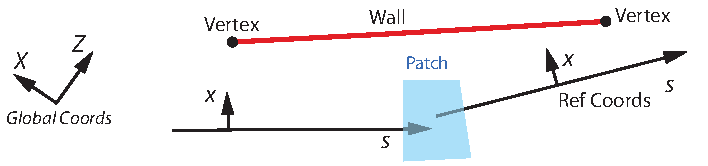
\includegraphics[width=5in]{patch.pdf}
  \caption[Standard patch transformation.]
{Standard tracking through a patch element. A particle's starting coordinate at the entrance end of
the patch has, by construction, coordinate $z$ = 0. The particle is drifted, as in a field free
region, between the entrance $z = 0$ plane and the exit $z = 0$ plane.}
  \label{f:patch.track}
\end{figure}

%---------------------------------------------------------------------------------

The transformation of the reference coordinates through a ``standard'' patch (a patch where custom
fields are not used) is given by \Eqs{vwlv} and \eq{wws}. At the entrance end of the patch, a
particle's position and momentum in the entrance coordinate system will be
\begin{alignat}{1}
  \bfr &= (x, y, 0) \CRNO
  \bfP &= (P_x, P_y, P_z) = 
    \left( p_x, p_y, \pm \sqrt{(1+p_z)^2 - p_x^2 - p_y^2} \right) \, P_{0\text{ent}}
\end{alignat}
where $p_x$, $p_y$ and $p_z$ are the phase space momenta, and $z$, which is coordinate $z$ and not
phase space $z$, is always zero by construction as shown in \fig{f:patch.track} [Also see
\fig{f:local.coords} and the discussion in \sref{s:phase.space}.] The sign of the longitudinal
momentum $P_z$ is determined by whether the particle is traveling in the positive $s$ or negative
$s$ direction (which will occur when an element is flipped longitudinally).

The transformation between entrance and exit coordinate systems is given by \Eqs{rwlr} and \eq{pps}
\begin{alignat}{1}
  \bfr &\rightarrow 
    \bfS^{-1} \, (\bfr - \bfL_\text{off}) \CRNO
  \bfP &\rightarrow \bfS^{-1} \, \bfP
\end{alignat}
where $\bfL_\text{off}$ is given by \Eq{swww}

After this transformation, the particle must be propagated by a longitudinal length
$-r_z$ to intersect the $r_z = 0$ plane of the exit face.
\begin{alignat}{1}
  \bfr &\rightarrow (r_x - r_z \, \frac{P_x}{P_z}, r_y - r_z \, \frac{P_y}{P_z}, 0) \CRNO
  \bfP &\rightarrow \bfP
\end{alignat}

The final $\bfr$ and $\bfP$ can now be used compute the particles
phase space coordinates, along with the time $t$ and the reference time
$t_\REF$ at the exit end.
\begin{alignat}{3}
  x &\rightarrow r_x \qquad &p_x &\rightarrow \frac{P_x}{P_{0\text{exi}}} \CRNO
  y &\rightarrow r_y \qquad &p_y &\rightarrow \frac{P_y}{P_{0\text{exi}}} \\
  z &\rightarrow z + r_z \, \frac{|\bfP|}{P_z} + L_0 \, \frac{\beta}{\beta_0} +
    \beta \, \text{t_offset} \qquad
    &p_z &\rightarrow \frac{(1+p_z) \, P_{0\text{ent}} - P_{0\text{exi}}}{P_{0\text{exi}}} \CRNO
  t &\rightarrow t - r_z \, \frac{|\bfP|}{P_z \, \beta} \qquad
  &t_\REF &\rightarrow t_\REF + \text{t_offset} + L_0 \, \frac{1}{\beta_0} \nonumber
\end{alignat}
where the exit reference momentum $P_{0\text{exi}}$ is related to the
entrance reference momentum $P_{0\text{ent}}$ through
\vn{e_tot_offset}.  In the above equation, $\beta$ is the particle
velocity, $\beta_0$ is the velocity of the reference particle, and
$L_0$ is the drift length of the reference particle
\begin{equation}
  L_0 = \frac{1}{S^{-1}_{33}} \, \left( 
  S^{-1}_{31} \, \text{x_offset} + S^{-1}_{32} \, \text{y_offset} + S^{-1}_{33} \, \text{z_offset}
  \right)
\end{equation}

%---------------------------------------------------------------------------------
%---------------------------------------------------------------------------------
\section{Quadrupole Tracking}
\label{s:quadrupole.std}
\index{quadrupole}

The \vn{bmad_standard} calculates the transfer map through an upright
quadrupole and then transforms that map to the laboratory frame.

The Hamiltonian for an upright quadrupole is
\begin{equation}
  H = \frac{p_x^2 + p_y^2}{2 (1 + p_z)} + \frac{k_1}{2} (x^2 - y^2)
\end{equation}
This is simply solved
\begin{align}
  x_2    &= c_x \, x_1 + s_x \, \frac{p_{x1}}{1 + p_{z1}} \CRNO
  p_{x2} &= \tau_x \, \om^2 \, \, (1 + p_{z1}) \, s_x \, x_1 + c_x \, p_{x1} \CRNO
  y_2    &= c_y \, y_1 + s_y \, \frac{p_{y1}}{1 + p_{z1}} \CRNO
  p_{y2} &= \tau_y \, \om^2 \, \, (1 + p_{z1}) \, s_y \, y_1 + c_y \, p_{y1} \\
  z_2    &= z_1 + m_{511} \, x_1^2 + m_{512} \, x_1 \, p_{x1} + m_{522} \, p_{x1}^2 + 
                   m_{533} \, y_1^2 + m_{534} \, y_1 \, p_{y1} + m_{544} \, p_{y1}^2 \CRNO
  p_{z2} &= p_{z1} \nonumber
\end{align}
where 
\begin{equation}
  \om \equiv \sqrt{\frac{|k_1|}{1 + p_{z1}}}
\end{equation}
and
\begin{alignat}{6}
         &\hspace*{3ex}  && k_1 > 0          &\hspace*{3ex}& k_1 < 0 & \qqquad
         &\hspace*{3ex}  && k_1 > 0          &\hspace*{3ex}& k_1 < 0 \CRNO
     c_x &=   && \cos  (\om \, L) && \cosh (\om \, L) & \qqquad
     c_y &=   && \cosh (\om \, L) && \cos  (\om \, L) \CRNO
     s_x &=   && \frac{\sin  (\om \, L)}{\om} && \frac{\sinh (\om \, L)}{\om} & \qqquad
     s_y &=   && \frac{\sinh (\om \, L)}{\om} && \frac{\sin  (\om \, L)}{\om} \\
  \tau_x &=   && {-}1             && {+}1             & \qqquad
  \tau_y &=   && {+}1             && {-}1             \nonumber
\end{alignat}
with this
\begin{alignat}{2}
  m_{511} &= \frac{\tau_x \,\, \om^2}{4} \, (L - c_x \, s_x) & \qqquad
  m_{533} &= \frac{\tau_y \,\, \om^2}{4} \, (L - c_y \, s_y) \CRNO
  m_{512} &= \frac{-\tau_x \,\, \om^2}{2 \, (1 + p_{z1})} \, s_x^2 & \qqquad
  m_{534} &= \frac{-\tau_y \,\, \om^2}{2 \, (1 + p_{z1})} \, s_y^2 \\
  m_{522} &= \frac{-1}{4 \, (1 + p_{z1})^2} \, (L + c_x \, s_x) & \qqquad
  m_{544} &= \frac{-1}{4 \, (1 + p_{z1})^2} \, (L + c_y \, s_y) \nonumber
\end{alignat}

%---------------------------------------------------------------------------------
%---------------------------------------------------------------------------------
\section{RFcavity Tracking}
\label{s:rfcavity.std}
\index{rfcavity}

For tracking using something like \vn{runge_kutta}, with \vn{field_calc} set to \vn{bmad_standard},
the fields are modeled by the equations given in Sections~\sref{s:rf.fields} and \sref{s:rf.fringe}.

With \vn{bmad_standard} tracking, a kick-drift-kick model is used. The kick is a
pure energy kick (see equations in \sref{s:rfcav}) and the phase of the RF is calculated under the
assumption that the waveform moves at a phase velocity equal to the velocity of the reference
particle.

With \vn{bmad_standard} tracking, the transverse forces due to the RF are ignored. This is generally
a reasonable approximation when the acceleration is small as is standard in rings. \vn{Lcavity}
elements should be used in place of \vn{rfcavity} elements when this is not so.

%---------------------------------------------------------------------------------
%---------------------------------------------------------------------------------
\section{Sad\_Mult Tracking}
\label{s:sad.mult.std}
\index{sad_mult}

The ``hard edge'' fringe field kick is taken from Forest\cite{b:forest} Eqs.~(13.29) and onward.
In the notation of \bmad, and taking into account both normal and skew terms, Eq.~(13.29)
is for the $m$\th order multipole (what Forest labels $n+1$)
\begin{equation}
  f_\pm = \mp \Re \frac{(b_m + i \, a_m) \, (x + i \, y)^{(m+1)}}{4 \, (m+2) \, (1 + p_z)}
    \left[ x \, p_x + y \, p_y + i\frac{m+3}{m+1}(x \, p_y - y \, p_x) \right]
\end{equation}

The ``soft edge'' dipole fringe for \vn{sad_mult} elements is a generalization of the soft edge
dipole fringe for a SAD bend element. For the entrance kick the equations are:
\begin{align}
  x_2 &= x_1 + \frac{\delta_1}{1 + \delta_1} \, \Delta x_{fx}, \qquad
  p_{x2} = p_{x1} + \frac{1}{1 + \delta_1} \, \left[ 
    \Delta x_{fy} \, v - \Delta x_{fay} \, v^3 \right] \CRNO
  y_2 &= y_1 - \frac{\delta_1}{1 + \delta_1} \, \Delta y_{fy}, \qquad
  p_{y2} = p_{y1} + \frac{1}{1 + \delta_1} \, \left[ 
    \Delta y_{fx} \, w - \Delta y_{fax} \, w^3 \right] \\
  z_2 &= z_1 + \frac{1}{(1 + \delta_1)^2} \, \left[ \, 
    \Delta x_{fx} \, p_{x1} - \Delta y_{fy} \, p_{y1} + 
    \frac{1}{2} \, (\Delta y_{fx} + \Delta x_{fy}) \, w^2 -
    \frac{1}{4} (\Delta y_{fax} + \Delta x_{fay}) \, w^4
    \right] \nonumber
\end{align}
where
\begin{alignat}{3}
  \Delta x_{fx}  &= \frac{K_0 \, F_B^2}{24 \, L}, & \qquad 
  \Delta y_{fx}  &= \frac{K_0^2 \, F_B}{6 \, L^2}, & \qquad 
  \Delta y_{fax} &= \frac{2 \, K_0^2}{3 \, F_B \, L^2}, \CRNO 
  \Delta y_{fy}  &= \frac{SK_0 \, F_B^2}{24 \, L}, & \qquad
  \Delta x_{fy}  &= \frac{SK_0^2 \, F_B}{6 \, L^2}, & \qquad
  \Delta x_{fay} &= \frac{2 \, SK_0^2}{3 \, F_B \, L^2}, \\
  v &= \cos\theta \, x_1 + \sin\theta \, y_1, & \qquad
  w &= -\sin\theta \, x_1 + \cos\theta \, y_1, & \qquad
  \tan\theta &= \frac{-SK_0}{K_0} \nonumber
\end{alignat}


%---------------------------------------------------------------------------------
%---------------------------------------------------------------------------------
\section{Sextupole Tracking}
\label{s:sextupole.std}
\index{sextupole}

The Hamiltonian for an upright sextupole is
\begin{equation}
  H = \frac{p_x^2 + p_y^2}{2 (1 + p_z)} + \frac{k_2}{6} (x^3 - 3 \, x \, y^2)
\end{equation}

Tracking through a sextupole uses a kick-drift-kick model.

%---------------------------------------------------------------------------------
%---------------------------------------------------------------------------------
\section{Sol\_Quad Tracking}
\label{s:sol.quad.std}
\index{sol_quad}

The Hamiltonian is
\begin{equation}
  H = \frac{(p_x + \frac{k_s }{2}\, y)^2}{2 (1 + p_z)} + 
  \frac{(p_y - \frac{k_s}{2} \, x)^2}{2 (1 + p_z)} + \frac{k_1}{2} (x^2 - y^2)
\end{equation}
Solving the equations of motion gives
\begin{align}
  x_2    &= m_{11} \, x_1 + m_{12} \, p_{x1} + m_{13} \, y_1 + m_{14} \, p_{y1} \CRNO
  p_{x2} &= m_{21} \, x_1 + m_{22} \, p_{x1} + m_{23} \, y_1 + m_{24} \, p_{y1} \CRNO
  y_2    &= m_{31} \, x_1 + m_{32} \, p_{x1} + m_{33} \, y_1 + m_{34} \, p_{y1} \CRNO
  p_{y2} &= m_{41} \, x_1 + m_{42} \, p_{x1} + m_{43} \, y_1 + m_{44} \, p_{y1} \\
  z_2    &= z_1 + \sum_{j = 1}^4 \sum_{k = j}^4 m_{5jk} \, r_j \, r_k  \CRNO
  p_{z2} &= p_{z1} \nonumber
\end{align}
where
\begin{alignat}{2}
  m_{11} &= \frac{1}{2 \, f} \, \left( f_{0+} \, c + f_{0-} \, c_h \right) & \qqquad
  m_{31} &= -m_{24} \CRNO
  m_{12} &= \frac{1}{2 \, f \, (1 + p_{z1})} \, 
            \left( \frac{f_{++}}{\om_+} \,  s + \frac{f_{--}}{\om_-} \, s_h \right) & \qqquad
  m_{32} &= -m_{14} \CRNO
  m_{13} &= \frac{\ks}{4 \, f} \, 
            \left( \frac{f_{+-}}{\om_+} \, s +\frac{f_{-+}}{\om_-} \, s_h \right) & \qqquad
  m_{33} &= \frac{1}{2 \, f} \, \left( f_{0-} \, c + f_{0+} \, c_h \right) \CRNO
  m_{14} &= \frac{\ks}{f \, (1 + p_{z1})} \, \left( -c + c_h \right) & \qqquad
  m_{34} &= \frac{1}{2 \, f \, (1 + p_{z1})} \, 
            \left( \frac{f_{+-}}{\om_+} \, s + \frac{f_{-+}}{\om_-} \, s_h \right) \CRNO
  m_{21} &= \frac{-(1 + p_{z1})}{8 \, f} \, 
            \left( \frac{\xi_{1+}}{\om_+} \, s + \frac{\xi_{2+}}{\om_-} s_h \right) & \qqquad
  m_{41} &= -m_{23} \\
  m_{22} &= m_{11} & \qqquad
  m_{42} &= -m_{13} \CRNO
  m_{23} &= \frac{\ks^3 \, (1 + p_{z1})}{4 \, f} \, \left( c - c_h \right) & \qqquad
  m_{43} &= \frac{-(1 + p_{z1})}{8 \, f} \, 
            \left( \frac{\xi_{1-}}{\om_+} \, s + \frac{\xi_{2-}}{\om_-} \, s_h \right) \CRNO
  m_{24} &= \frac{\ks}{4 \, f} \, 
            \left( \frac{f_{++}}{\om_+} \, s + \frac{f_{--}}{\om_-} \, s_h \right) & \qqquad
  m_{44} &= m_{33} \nonumber
\end{alignat}
and
\begin{alignat}{2}
  \kone        &= \frac{k_1}{1 + p_{z1}} & \qqquad 
  \ks          &= \frac{k_s}{1 + p_{z1}} \CRNO
  f            &= \sqrt{\ks^4 + 4 \, \kone^2} & \qqquad
  f_{\pm0}     &= f \pm \ks^2 \CRNO
  f_{0\pm}     &= f \pm 2 \, \kone & \qqquad
  f_{\pm\pm}   &= f \pm \ks^2 \pm 2 \, \kone \CRNO
  \om_+        &= \sqrt{\frac{f_{+0}}{2}} & \qqquad
  \om_-        &= \sqrt{\frac{f_{-0}}{2}} \\
  s            &= \sin (\om_+ \, L) & \qqquad
  s_h          &= \sinh (\om_- \, L) \CRNO
  c            &= \cos (\om_+ \, L) & \qqquad
  c_h          &= \cosh (\om_- \, L) \CRNO
  \xi_{1\pm} &= \ks^2 \, f_{+\mp} \pm 4 \, \kone \, f_{+\pm} & \qqquad
  \xi_{2\pm} &= \ks^2 \, f_{-\pm} \pm 4 \, \kone \, f_{-\mp} \nonumber
\end{alignat}

The $m_{5jk}$ terms are obtained via \Eq{zz121p}
\begin{align}
  m_{5jk} = - \frac{\tau_{jk}}{2 (1 + p_{z1})^2} \int \! ds \, 
  & \left[ 
    \left( m_{2j} + \frac{k_s}{2} \, m_{3j} \right) \, 
    \left( m_{2k} + \frac{k_s}{2} \, m_{3k} \right)   
  \right. + \\
  & \hspace*{15ex} \left.
    \left( m_{4j} - \frac{k_s}{2} \, m_{1j} \right) \, 
    \left( m_{4k} - \frac{k_s}{2} \, m_{1k} \right) 
  \right] \nonumber
\end{align}
where
\begin{equation}
  \tau_{jk} = 
  \begin{cases}
    1 & j = k \\
    2 & j \ne k 
  \end{cases}
\end{equation}
The needed integrals involve the product of two trigonometric or
hyperbolic functions. These integrals are trivial to do but the
explicit equations for $m_{5jk}$ are quite long and in the interests of
brevity are not reproduced here.

%---------------------------------------------------------------------------------

\begin{figure}[tb]
  \centering
  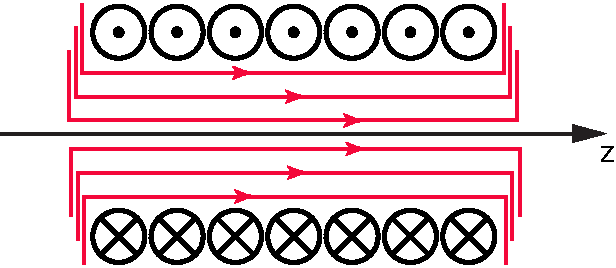
\includegraphics[width=5in]{solenoid.pdf}
  \caption[Solenoid with a hard edge.]
  {
Solenoid with a hard edge. The field is assumed to end abruptly at the edges of the solenoid. Here,
for purposes of illustration, the field lines at the ends are displaced from one another.
  }
  \label{f:solenoid}.
\end{figure}

%---------------------------------------------------------------------------------
\section{Solenoid Tracking}
\label{s:solenoid.std}
\index{solenoid}

The \vn{bmad_standard} solenoid tracking does not make the small angle approximation.
The transfer map for the solenoid is:
\begin{align}
  x_2    &= \frac{1 + c}{2} \, x_1 + \frac{s}{k_s} \, p_{x1} +
           \frac{s}{2} \, y_1 + \frac{1 - c}{k_s} \, p_{y1} \CRNO
  p_{x2} &= \frac{-k_s \, s}{4} \, x_1 + \frac{1 + c}{2} \, p_{x1} - 
           \frac{k_s \, (1 - c)}{4} \, y_1 + \frac{s}{2} \, p_{y1} \CRNO
  y_2    &= \frac{-s}{2} \, x_1 - \frac{1 - c}{k_s} \, p_{x1} +
           \frac{1 + c}{2} \, y_1 + \frac{s}{k_s} \, p_{y1} \\      
  p_{y2} &= \frac{k_s \, (1 - c)}{4} \, x_1 + \frac{-s}{2} \, p_{x1} -
            \frac{k_s \, s}{4} \, y_1 + \frac{1 + c}{2} \, p_{y1} \CRNO 
  z_2    &= z_1 + \frac{L \, (1 + p_{z1})^2}{2 \, p_r^3} \, 
                   \left[ \left( p_{x1} + \frac{k_s}{2} \, y_1 \right)^2 +
                          \left( p_{y1} - \frac{k_s}{2} \, x_1 \right)^2 \right] \CRNO
  p_{z2} &= p_{z1} \nonumber
\end{align}
where $k_s = B/P_0$ is the normalized field and
\begin{align}
  c &= \cos \left( k_s L / p_r \right) \CRNO
  s &= \sin \left( k_s L / p_r \right)
\end{align}
with
\begin{equation}
  p_r = \sqrt{(1 + p_z)^2 - (p_x + y_1 \, k_s/2)^2 - (p_y - x_1 \, k_s/2)^2}
\end{equation}

To be useful, the canonical momenta $p_x$ and $p_y$ in the above equations must be connected to the
canonical momenta used for other elements (drifts, quadrupoles, etc.) that may be placed to either
side of the solenoid. These side elements use zero $a_x$ and $a_y$ (cf. \Eq{pmc2pc}). The vector
potential used in the solenoid canonical momenta may be made zero at the edges of the solenoid if
the solenoid fringe field is assumed to end abruptly at the edges of the solenoid (as shown in
\fig{f:solenoid}), and the reference axis $\Bf z$-axis (at $x$ = $y$ = 0) is placed along the
centerline of the solenoid so that there is cylindrical symmetry around the $\Bf z$-axis.

%-----------------------------------------------------------------------------------------
\section{Sprint Spin Tracking}
\label{s:sprint.std}
\index{sprint spin tracking}

The \vn{sprint} spin tracking method is named after the \vn{SPRINT} program developed by Matthias
Vogt.  The \vn{sprint} algorithm Uses a first order spin map evaluated with respect to the zero
orbit to track through elements. This method is much faster than PTC integration, and its run-time
does not increase proportionally to element length. Currently, the supported lattice elements are
bends (including bends with $k_1 \neq 0$), quadrupoles, and solenoids \sref{s:spin.methods}.

Elements with fringe field contributions are split into three quaternions representing the entrance,
body, and exit of the element. Before propagation, the exit fringe quaternion is always equivalent
to the entrance fringe quaternion, with all field strengths multiplied by -1, and $e_1$ replaced
with $-e_2$. The exit quaternion is then propagated to the end of the element via Bmad mapping
tools. Appropriate quaternions are concatenated according to the values of \vn{spin_fringe_on} and
\vn{fringe_at}.

\begin{alignat}{8}
 & {d}    &&= g \, l              && {e}    &&= a \, g \, l\gamma   && s     &&= a \, k_s l       && {t}    &&= (1+a) k_s l         \CRNO
 & c_{d}  &&= \cos({d})    \qquad && s_{e2} &&= \sin(\frac{{e}}{2}) && c_{s} &&= \cos({s}) \qquad && c_{t}  &&= \cos({t})           \\
 & s_{d}  &&= \sin({d})           && c_{e2} &&= \cos(\frac{{e}}{2}) && s_{s} &&= \sin({s})        && s_{t2} &&= \sin(\frac{{t}}{2}) \CRNO
 & \chi   &&= 1+a\gamma           && \zeta  &&= \gamma - 1   \qquad && \psi  &&= \gamma^2 - 1     && c_{t2} &&= \cos(\frac{{t}}{2}) \nonumber
\end{alignat}

%-----------------------------------------------------------------------------------------
\subsection{SBend Body, $k_1 = 0$}

\begin{center}
\begin{tabular}{llll} \toprule
        & $q_0$    & $q_y$     & $q_z$ \\ \midrule
  $1$   & $c_{e2}$ & $-s_{e2}$ &       \\ \addlinespace[1ex]
  $x$   & $-\frac{1}{2} g \chi s_{d} s_{e2}$ & $-\frac{1}{2} g \chi \, s_{d} c_{e2}$ & \\ \addlinespace[1ex]
  $p_x$ & $\frac{1}{2} \chi \, (c_{d} - 1)  s_{e2}$ & $\frac{1}{2} \chi \, (c_{d} - 1) c_{e2}$ & \\ \addlinespace[1ex]
  $p_y$ &          &           & $\frac{1}{\gamma} \zeta \, s_{e2}$ \\ \addlinespace[1ex]
  $p_z$ & $\frac{1}{2 \gamma} \left(\gamma \, \chi \, s_{d} -a \, \psi \, {d} \right) s_{e2}$ & & \\
  \bottomrule
\end{tabular}
\end{center}

%-----------------------------------------------------------------------------------------
\subsection{Sbend Body, $k_1 \neq 0$}

\begin{equation}
\begin{aligned}
  &  k_x = k_1 + g^2 \\
  & \omega_x = \sqrt{|k_x|} \\
  & \omega_y = \sqrt{|k_1|}
\end{aligned}
\qquad\qquad\qquad
\begin{aligned}
  & \alpha = 2(a^2 g^2 \gamma^2 + k_1) \\ \nonumber
  & \beta = a g k_1 (\gamma \chi - \zeta) \\ \nonumber
  & \sigma = \omega_y (k_1 + a k_1 \gamma + a^2g^2 \zeta \gamma)\\ \nonumber
  & \xi = \omega_y (k_1 \chi + a^2 g^2 \zeta \gamma) \nonumber
\end{aligned}
\end{equation}

\begin{center}
\begin{tabular}{cccc}
  $k_x > 0$                  & $k_x < 0$              & $k_1 > 0$                   & $k_1 < 0$  \\
  $s_x = \sin{(l \omega_x)}$ & $ \sinh{(l \omega_x)}$ & $s_y = \sinh{(l \omega_y)}$ & $ \sin{(l \omega_y)}$ \\
  $c_x = \cos{(l \omega_x)}$ & $ \cosh{(l \omega_x)}$ & $c_y = \cosh{(l \omega_y)}$ & $ \cos{(l \omega_y)}$ \\
  $\tau_x = -1$              & $+1$                   & $\tau_y = +1$               & $-1$
\end{tabular}
\end{center}

\begin{center}
\begin{tabular}{lllll} \toprule
        & $q_0$    & $q_x$ & $q_y$     & $q_z$ \\ \midrule
  1     & $c_{e2}$ &       & $-s_{e2}$ &       \\ \addlinespace[1ex]
  $x$   & $\frac{-k_x \chi}{2 \omega_x} s_x s_{e2}$            &   &
    $\frac{-k_x \chi}{2 \omega_x} s_x c_{e2}$ & \\ \addlinespace[1ex]
  $p_x$ & $\frac{k_x \chi}{2\omega_x^2} \tau_x (1-c_x) s_{e2}$ &   &
    $\frac{k_x \chi}{2 \omega_x^2} \tau_x \left(1-c_x\right) c_{e2}$ & \\ \addlinespace[1ex]
  $y$   &          &
    {$\begin{aligned}
      \frac{-1}{\alpha} &\bigl[ \beta (1+ c_y) s_{e2} +{} \\[-1.5ex]
      & \hskip4.5em \tau_y \sigma s_y c_{e2} \bigr]
    \end{aligned}$} &  &
    {$\begin{aligned}
       \frac{1}{\alpha} &\bigl[ \beta (1-c_y) c_{e2} + {} \\[-1.5ex]
       & \hskip4.5em \tau_y \sigma s_y s_{e2} \bigr]
    \end{aligned}$} \\ \addlinespace[1ex]
  $p_y$ &          &
    {$\begin{aligned}
      \frac{1}{\omega_y \alpha} &\bigl[ \xi (1 - c_y) c_{e2} - {} \\[-1.5ex]
      & \hskip5em \beta s_y s_{e2} \bigr]
    \end{aligned}$} &   &
    {$\begin{aligned}
      \frac{1}{\omega_y \alpha} &\bigl[ \xi (1+c_y) s_{e2} - {} \\[-1.5ex]
      & \hskip5em \beta s_y c_{e2}\bigr]
    \end{aligned}$} \\ \addlinespace[1ex]
  $p_z$ & $\frac{g}{2}\left(\frac{\chi s_x}{\omega_x} - \frac{a l \psi}{\gamma}\right) s_{e2}$ &    &
    $\frac{g}{2}\left(\frac{\chi s_x}{\omega_x} - \frac{a l \psi}{\gamma}\right) c_{e2}$ & \\
  \bottomrule
  \end{tabular}
\end{center}

%-----------------------------------------------------------------------------------------
\subsection{Sbend Entrance Fringe}

To calculate the exit fringe, multiply all field strengths $g$ by
-1, and replace all entrance face angles $e_1$ with exit face angles $-e_2$. The negative exit face
angle is used due to Bmad convention.
\begin{center}
  \begin{tabular}{lllll} \toprule
      & $q_0$ & $q_x$                         & $q_y$                          & $q_z$ \\ \midrule
  1   & 1     &                               &                                & \\ \addlinespace[1ex]
  $x$ &       &                               & $\frac{1}{2} \chi g \tan(e_1)$ & \\ \addlinespace[1ex]
  $y$ &       & $\frac{1}{2}(1+a)g \sin(e_1)$ &                                & $-\frac{1}{2}(1+a)g \cos(e_1)$ \\
  \bottomrule
  \end{tabular}
\end{center}

%-----------------------------------------------------------------------------------------
\subsection{Quadrupole}

\begin{equation}
  \omega = \sqrt{|k_1|} \nonumber
\end{equation}

\begin{center}
\begin{tabular}{cccc}
  $k_1 > 0$ & $k_1 < 0$ & $k_1 > 0$ & $k_1 < 0$  \\
  $s_x = \frac{\sin{(l \omega)}}{\omega}$ & $ \frac{\sinh{(l \omega)}}{\omega}$ &$s_y = \frac{\sinh{(l \omega)}}{\omega}$ & $ \frac{\sin{(l \omega)}}{\omega}$ \\
  $c_x = \frac{1 - \cos{(l \omega)}}{\omega^2}$ & $ \frac{-1 + \cosh{(l \omega)}}{\omega^2}$ &$c_y = \frac{-1 + \cosh{(l \omega)}}{\omega^2}$ & $ \frac{1 - \cos{(l \omega)}}{\omega^2}$ \\
\end{tabular}
\end{center}
\everymath{}

\begin{center}
\begin{tabular}{llll} \toprule
        & $q_0$ & $q_x$ & $q_y$ \\ \midrule
  1     & 1     &       &       \\ \addlinespace[1ex]
  $x$   &       &       & $-\frac{1}{2} k_1 \chi s_x$ \\ \addlinespace[1ex]
  $p_x$ &       &       & $-\frac{1}{2} k_1 \chi c_x$ \\ \addlinespace[1ex]
  $y$   &       & $-\frac{1}{2} k_1 \chi s_y$ & \\ \addlinespace[1ex]
  $p_y$ &       & $-\frac{1}{2} k_1 \chi c_y$ & \\
\bottomrule
\end{tabular}
\end{center}

%-----------------------------------------------------------------------------------------
\subsection{Solenoid Element Body}

\begin{center}
\begin{tabular}{lllll} \toprule
  &  $q_0$ & $q_x$ & $q_y$ & $q_z$ \\ \midrule
  1 & $c_{t2}$ & & & $-s_{t2}$ \\ \addlinespace[1ex]
  $x$ & & $\frac{1}{4} k_s \zeta ((1 - c_{s}) c_{t2} - s_{s} s_{t2})$ & $\frac{1}{4} k_s \zeta ((-1 + c_{s}) s_{t2} - s_{s} c_{t2})$ & \\ \addlinespace[1ex]
  $p_x$ & & $\frac{1}{2} \zeta ((1-c_{s}) {st2} + s_{s} c_{t2})$ & $\frac{1}{2} \zeta ((1 - c_{s}) c_{t2} - s_{s} s_{t2})$ & \\ \addlinespace[1ex]
  $y$ & & $\frac{1}{4} k_s \zeta ((1 - c_{s}) s_{t2} + s_{s} c_{t2})$ & $\frac{1}{4} k_s \zeta ((1 - c_{s}) c_{t2} - s_{s} s_{t2})$ &\\ \addlinespace[1ex]
  $p_y$ & & $\frac{1}{2} \zeta ((-1 + c_{s}) c_{t2} + s_{s} s_{t2})$ & $\frac{1}{2} \zeta ((1-c_{s}) s_{t2} + s_{s} c_{t2})$ & \\ \addlinespace[1ex]
  $p_z$ & $\frac{1}{2} {t} s_{t2}$ & & & $\frac{1}{2} {t} c_{t2}$ \\
\bottomrule
\end{tabular}
\end{center}

%-----------------------------------------------------------------------------------------
\subsection{Solenoid Entrance Fringe}
To calculate the exit fringe, multiply all field strengths $k_s$ by -1.
\begin{center}
\begin{tabular}{llll} \toprule
  & $q_0$ & $q_x$ & $q_y$ \\ \midrule
  1 & 1 & & \\
  $x$ & & $\frac{1}{4} k_s \chi $ &  \\
  $y$ & & & $\frac{1}{4} k_s \chi $ \\
\bottomrule
\end{tabular}
\end{center}

%---------------------------------------------------------------------------------
\section{Symplectic Tracking with Cartesian Modes}
\label{s:wiggler.std}
\index{wiggler!tracking}

The method for symplectic integration for elements that define the magnetic field using a
Cartesian mode decomposition (\sref{s:cart.map}) is outlined in \sref{s:symp.track}.  The
vector potential is constructed to avoid singularities when one of the wave vectors $k_x$,
$k_y$, or $k_z$ is zero.

For the \vn{x} \vn{family} the vector potential is:
\begin{center}
{
\setlength{\tabcolsep}{1pt}
\begin{tabular}{lrllrllrll}
  Form \; & \multicolumn{3}{l}{hyper-y}  & \multicolumn{3}{l}{hyper-xy}  & \multicolumn{3}{l}{hyper-x} \\
  $A_x$   & 
    $A$ & $\dfrac{k_z}{k_y^2}$      & $\Se_x \, \Sh_y \, \Se_z \qquad$ &
    $A$ & $\dfrac{1}{k_y}$          & $\Sh_x \, \Sh_y \, \Se_z \qquad$ &
    $A$ & $\dfrac{k_z}{k_x \, k_y}$ & $\Sh_x \, \Se_y \, \Se_z$ \\
  $A_y$   & 0 &&& 0 &&& 0 && \\
  $A_z$   & 
    $A$ & $\dfrac{k_x}{k_y^2}$      & $\Ce_x \, \Sh_y \, \Ce_z \qquad$ &
    $A$ & $\dfrac{k_x}{k_y \, k_z}$ & $\Ch_x \, \Sh_y \, \Ce_z \qquad$ &
    $A$ & $\dfrac{1}{k_y}$          & $\Ch_x \, \Se_y \, \Ce_z$ 
\end{tabular}
}
\end{center}

For the \vn{y} \vn{family} the vector potential is:
\begin{center}
{
\setlength{\tabcolsep}{1pt}
\begin{tabular}{lrllrllrll}
  Form \; & \multicolumn{3}{l}{hyper-y}  & \multicolumn{3}{l}{hyper-xy}  & \multicolumn{3}{l}{hyper-x} \\
  $A_x$   & 0 &&& 0 &&& 0 && \\
  $A_y$   & 
    $-A$ & $\dfrac{k_z}{k_x \, k_y}$ & $\Se_x \, \Sh_y \, \Se_z \qquad$ &
    $-A$ & $\dfrac{1}{k_x}$          & $\Sh_x \, \Sh_y \, \Se_z \qquad$ &
    $-A$ & $\dfrac{k_z}{k_x^2}$      & $\Sh_x \, \Se_y \, \Se_z$ \\
  $A_z$   & 
    $-A$ & $\dfrac{1}{k_x}$          & $\Se_x \, \Ch_y \, \Ce_z \qquad$ &
    $-A$ & $\dfrac{k_y}{k_x \, k_z}$ & $\Sh_x \, \Ch_y \, \Ce_z \qquad$ &
    $-A$ & $\dfrac{k_y}{k_x^2}$      & $\Sh_x \, \Ce_y \, \Ce_z$ 
\end{tabular}
}
\end{center}

For the \vn{qu} \vn{family} the vector potential is:
\begin{center}
{
\setlength{\tabcolsep}{1pt}
\begin{tabular}{lrllrllrll}
  Form \; & \multicolumn{3}{l}{hyper-y}  & \multicolumn{3}{l}{hyper-xy}  & \multicolumn{3}{l}{hyper-x} \\
  $A_x$   & 
     $A$ & $\dfrac{1}{k_z}$          & $\Se_x \, \Ch_y \, \Se_z \qquad$ &
     $A$ & $\dfrac{k_y}{k_z^2}$      & $\Sh_x \, \Ch_y \, \Se_z \qquad$ &
     $A$ & $\dfrac{k_y}{k_x \, k_z}$ & $\Sh_x \, \Ce_y \, \Se_z$ \\
  $A_y$   & 
    $-A$ & $\dfrac{k_x}{k_y \, k_z}$ & $\Ce_x \, \Sh_y \, \Se_z \qquad$ &
    $-A$ & $\dfrac{k_x}{k_z^2}$      & $\Ch_x \, \Sh_y \, \Se_z \qquad$ &
    $-A$ & $\dfrac{1}{k_z}$          & $\Ch_x \, \Se_y \, \Se_z$ \\
  $A_z$   & 0 &&& 0 &&& 0 &&
\end{tabular}
}
\end{center}

For the \vn{sq} \vn{family} the vector potential is:
\begin{center}
{
\setlength{\tabcolsep}{1pt}
\begin{tabular}{lrllrllrll}
  Form \; & \multicolumn{3}{l}{hyper-y}  & \multicolumn{3}{l}{hyper-xy}  & \multicolumn{3}{l}{hyper-x} \\
  $A_x$   & 
     $A$ & $\dfrac{1}{k_z}$          & $\Ce_x \, \Sh_y \, \Se_z \qquad$ &
     $A$ & $\dfrac{k_y}{k_z^2}$      & $\Ch_x \, \Sh_y \, \Se_z \qquad$ &
     $A$ & $\dfrac{k_y}{k_x \, k_z}$ & $\Ch_x \, \Se_y \, \Se_z$ \\
  $A_y$   & 
     $A$ & $\dfrac{k_x}{k_y \, k_z}$ & $\Se_x \, \Ch_y \, \Se_z \qquad$ &
    $-A$ & $\dfrac{k_x}{k_z^2}$      & $\Sh_x \, \Ch_y \, \Se_z \qquad$ &
     $A$ & $\dfrac{1}{k_z}$          & $\Sh_x \, \Ce_y \, \Se_z$ \\
  $A_z$   & 0 &&& 0 &&& 0 &&
\end{tabular}
}
\end{center}


\chapter{Tracking of X-Rays}
\label{c:xray.track}

\bmad can track both charged particles and X-rays. This chapter deals
with X-rays. Charged particles are handled in chapter~\sref{c:charged.track}.

%-------------------------------------------------------------------------
%-------------------------------------------------------------------------
\section{Coherent and Incoherent Photon Simulations}
\label{s:coher.incoher}

\index{coherent tracking}\index{incoherent tracking}
\bmad can track photons either \vn{coherently} or \vn{incoherently}.
In both cases, the photon has a transverse electric field 
\begin{equation}
  (E_x, E_y)
\end{equation}
$E_x$ and $E_y$ are complex and therefore have both amplitude and phase information. When photons
are tracked incoherently, the phase information is not used for calculating X-ray intensities.

In addition to coherent and incoherent tracking, partially coherent simulations can be done by using
sets of photons with the photons in any one set treated as coherent and the photons between sets
being treated as incoherent.

%-------------------------------------------------------------------------
\subsection{Incoherent Photon Tracking}
\label{s:incoher}

In a simulation with incoherent photons, some number of photons,
$N_0$, will be generated and the i\Th photon ($i = 1, \ldots, N_0)$
will have a initial ``electric field'' components $E_{x0}(i),
E_{y0}(i)$ assigned to it. The field amplitude $E_0$ will be
$\sqrt{E_{x0}^2 + E_{y0}^2}$.

At some an observation point, the power $S$ per unit area falling on
some small area $dA$ due to either $x$ or $y$ component of the
electric field is
\begin{equation}
  S_{x,y} = \frac{\alpha_p}{N_0 \, dA} \, \sum_{j \in \text{hits}} E_{x,y}^2(j)
  \label{panda1}
\end{equation}
where $\alpha_p$ is a constant that can be chosen to fit the
simulation against experimental results, and the sum is over photons
who intersect the area. The factors of $N_0$ and $dA$ in the above
equation make, within statistical fluctuations, $S$ independent of
$N_0$ and, for $dA$ small enough, $S$ will be independent of $dA$ as
it should be. The total power is just $S_x + S_y$.

When traveling through vacuum, the electric field of a photon is a
constant.  As an example, consider a point source radiating uniformly
in $4\pi$ solid angle with each photon having the same initial field
$E_0$. An observation area $dA$ situated a distance $R$ from the
source will intercept $N_0 \, dA / 4 \, \pi \, R^2$ photons which
gives a power of
\begin{equation}
  S_w = \frac{\alpha_p \, E_0^2}{4 \, \pi \, R^2}
\end{equation}
which falls off as $1/R^2$ as expected.

At some places the light may be split into various ``channels''. An
example is Laue diffraction where X-rays can excite the $\alpha$ and
$\beta$ branches of the dispersion surface. Or a partially silvered
mirror where some of the light is reflected and some is transmitted.
In such a case, the probability $P_i$ of a photon traveling down the
$i$\Th channel is
\begin{equation}
  P_i \, \what E_i^2 = \frac{S_i}{S_0}
  \label{rpss1}
\end{equation}
where $S_i$ is the power flowing into channel $i$, $S_0$ is the power
flowing into the junction, and $\what E_i = E_i / E_0$ is the ratio of
the electric field amplitudes of any photon just before and just after being
shunted into the $i$\Th channel. The probabilities must be properly
normalized
\begin{equation}
  \sum P_i = 1
  \label{p1}
\end{equation}

If the ratio of the electric field of any photon just before and just
after being shunted into the $i$\Th channel is not a constant, than
$\what E_i$ must be adjusted so that $\what E_i^2$ is equal to the average of
$\what E_i^2(j)$ for all photons $j$ channeled into channel $i$.

As long as \Eqs{rpss1} and \eq{p1} are satisfied, the choice of the
$P_i$, and $\what E_i$ are arbitrary. This freedom allows simulation to be
optimized for efficiency. For example, In an actual experiment much of
the light can be lost never to reach a detector and be counted. To
decrease the simulation time, simulated photons may be limited to be
generated with a direction to be within some solid angle $\Omega_1$ if
photons with a direction outside this solid angle will not contribute
to the simulation results. In this case, there are two channels.
Channel 1 consists of all photons whose direction is within
$\Omega_1$ and channel 2 is all the other photons. To limit the
photons to channel 1, $P_1$ is taken to be 1 and $P_2$ is taken to be
0. Additionally, if the light, say, is being generated isotropically
from a surface into a $\Omega_0 = 2 \, \pi$ solid angle then
\begin{equation}
  \what E_1 = \sqrt{\frac{\Omega_1}{\Omega_0}}
  \label{roo}
\end{equation}
$\what E_2$ is infinite here but since no photons are generated in channel 2
this is not a problem.

%-------------------------------------------------------------------------
\subsection{Coherent Photon Tracking}
\index{ss:coher}

In a simulation with coherent photons, some number of photons,
$N_0$, will be generated and the i\Th photon ($i = 1, \ldots, N_0)$
will have an initial electric field $E_{x0}(i), E_{y0}(i)$ assigned to
it. These quantities will be complex.

At some an observation point, the field $E$ at
some small area $dA$ due to either $x$ or $y$ component of the
electric field is
\begin{equation}
  E = \frac{\alpha_p}{N_0 \, dA} \, \sum_{j \in \text{hits}} E(j)
  \label{panda2}
\end{equation}
where $\alpha_p$ is a constant that can be chosen to fit the
simulation against experimental results, and the sum is over photons
who intersect the area. In the above equation $E(j)$ is either the $x$
or $y$ component of the electric field as is appropriate. The factors
of $N_0$ and $dA$ in the above equation make, within statistical
fluctuations, $E$ independent of $N_0$ and, for $dA$ small enough, $E$
will be independent of $dA$ as it should be.

When traveling through a a vacuum, the photons travel ballistically in
straight lines. This is justified by using the stationary phase
approximation with Kirchhoff's integral. the electric field of a
photon varies with the propagation length. There is nothing physical
in this and is just a way to make the bookkeeping come out
correctly. As an example, consider a point source radiating uniformly
in $4\pi$ solid angle with each photon having the same initial field
component (either $x$ or $y$) $E_1$.  An observation area $dA$
situated a distance $R$ from the source will intercept $N_0 \, dA / 4
\, \pi \, R^2$ photons and each photon will have a field of $E_1 \, R
\, \exp(i \, k \, R)$ where $k$ is the photon wave number (all photons
must have the same $k$ to be coherent). This gives an electric field
at the observation point of
\begin{equation}
  E = \frac{\alpha_p \, E_1 \, \exp(i \, k \, R)}{4 \, \pi \, R}
\end{equation}
which falls off as $1/R$ as expected.

At a \vn{diffraction_plate} element where diffraction effects are to
be simulated, the following procedure is used:
  \begin{enumerate}
  \item
The electric field components are multiplied by the propagation length $L$:
\begin{equation}
  E \rightarrow E \, L
\end{equation}
The propagation length is reset to zero so that the at the next point
where the propagation length is factored into the electric field the
propagation length will be the length starting at the aperture.
  \item
Depending upon the program, the photon is is either given a random
direction over $2 \, \pi$ solid angle or the photon's direction
is restricted to be within some solid angle chosen to increase
the probability that the photon will make it through some downstream aperture.

If the photon is restricted to some aperture dependent solid angle of area $\Omega$,
the photon's electric field is scaled by
\begin{equation}
  E \rightarrow E \, \frac{\Omega}{4 \, \pi}
  \label{eeo4p}
\end{equation}

  \item
The electric field components are scaled by
\begin{equation}
  E \rightarrow E \, \frac{k}{4 \, \pi \, i} \, (\cos\theta_1 + \cos\theta_2)
  \label{eek4p}
\end{equation}
where $\theta_1$ and $\theta_2$ are the direction cosines of the
incoming and outgoing directions of the photon with respect to the
longitudinal reference axis.
  \end{enumerate}
This algorithm is designed so that the resulting fields at points
downstream from the aperture as computed from a simulation will, to
within statistical errors, be the same as one would get using
Kirchoff's integral. That is, the simulation is constructed to be a
Monte Carlo integration of Kirchhoff's integral.

What is, and what is not considered a place where there are
diffraction effects is dependent upon the problem. For example, there
are diffraction effects associated with light reflecting from a mirror
(or any other object) of finite size. If these effects are important
to the experiment, then a procedure similar to the one above must be
followed. 

At places where there are no diffraction effects a simulation can
treat the photons ballistically or can use the aperture procedure
outlined above. While in theory it is possible to choose what to do, in
practice the aperture procedure increases the number of photons that
must be tracked for a given resolution. Thus, from a practical standpoint
the ballistic alternative should always be used.

As explained in \sref{s:incoher}, at some places the light may be split
into various ``channels''. With coherent photons, the analog to \Eq{rpss1} is
\begin{equation}
  P_i \, \what E_i = \frac{E_i}{E_0}
  \label{rpss2}
\end{equation}
where here $\what E_i$ can be complex to take into account phase shifts.
The same considerations about choosing the $P_i$ and $\what E_i$ apply to
coherent photons as incoherent photons. In particular, $\what E_1$ for the
case of isotropic emission from a surface as in the example in
\sref{s:incoher} (cf. \Eq{roo}) is
\begin{equation}
  \what E_1 = \frac{\Omega_1}{\Omega_0}
\end{equation}

%-------------------------------------------------------------------------
\subsection{Partially Coherent Photon Simulations}

When there is partial coherence the photons must be divided into
sets. All of the photons of a given set are considered coherent while
the photons of different sets are treated incoherently.

The procedure is to track all the photons of one set coherently and
calculate the field using equation \Eq{panda2}. The fields of
different sets are then combined to calculate a power using
\Eq{panda1}.

%-------------------------------------------------------------------------
%-------------------------------------------------------------------------
\section{Element Coordinate System}
\label{s:photon.ele.coords}

\index{element coordinates}
The general procedure for tracking through an element makes use of
\vn{element reference} coordinates (also called just \vn{element}
coordinates). Without any offsets, pitches or tilt (\sref{s:offset}), henceforth
called ``misalignments'', the \vn{element} coordinates are the same
as the \vn{laboratory reference} coordinates (or simply \vn{laboratory}
coordinates) (\sref{s:ref}). The \vn{element} coordinates stay fixed
relative to the element. Therefore, if the element is misaligned, the
\vn{element coordinates} will follow as the element shifts in the
laboratory frame as shown in \fig{f:ele.coord}.

\index{crystal}\index{mirror}\index{multilayer_mirror}
For \vn{crystal} (\sref{s:crystal}), \vn{mirror} (\sref{s:mirror}), and \vn{multilayer_mirror}
(\sref{s:multilayer}) elements, the ``kinked'' reference trajectory through the element complicates
the calculation. For these elements, there are three coordinate systems attached to the element as
shown in \fig{f:photon.ele.coords}. Besides the \vn{element entrance} and \vn{element exit}
coordinates, there are \vn{element surface} coordinates with $z$ perpendicular to the surface
pointing inward.

Tracking a particle through an element is therefore a three
step transformation:
\begin{enumerate}[itemsep=-0.1ex, topsep=-0.4ex]
\item
At the entrance end of the element, transform from the laboratory
reference coordinates to the element's \vn{entrance} or \vn{surface}
coordinates.
\item
Track through the element ignoring any misalignments.
\item
At the exit end of the element, transform from the element coordinates
to the \vn{laboratory} \vn{exit} coordinates.
\end{enumerate}


%-------------------------------------------------------------------------

\begin{figure}[tb]
  \centering
  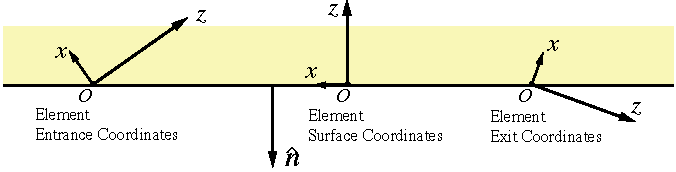
\includegraphics[width=5in]{photon-ele-coords.pdf}
  \caption[Crystal, Mirror, and Multilayer_Mirror Element Coordinates.]
{The three element coordinate systems for \vn{crystal} (Bragg
configuration), \vn{mirror}, and \vn{multilayer_mirror} elements.  The
origin $\Bf O$ of all three are the same but are shown spread out for
clarity.  $\bfhat n$ is the normal to the element surface.}
  \label{f:photon.ele.coords}.
\end{figure}

%-------------------------------------------------------------------------
\subsection{Transform from Laboratory Entrance to Element Coordinates}

For elements that have a reference orbit kink
(\sref{s:photon.ele.coords}), the element coordinates here are the
\vn{surface} coordinates. Otherwise the element coordinates are
the entrance coordinates.

  \begin{enumerate}
  \item
Apply offsets, pitches and tilt using the formulas in
\sref{s:pos.trans} along with \Eqs{wws}, and \eq{swww}.
  \item
Apply the \vn{tilt} to the electric field (\Eq{ertee}).
  \item
For \vn{crystal}, \vn{mirror}, and \vn{multilayer_mirror} elements
rotate to element surface coordinates.
 \item
Transform the photon's position as if in a drift by a distance $-z$
where $z$ is the photon's longitudinal coordinate. That is, $z$ will
be zero at the end of the transform to element coordinates (remember
that $z$ is the distance from the start of the element
(\sref{s:photon.phase.space})).

\end{enumerate}

%-------------------------------------------------------------------------
\subsection{Transform from Element Exit to Laboratory Coordinate}

The back transformation from element to laboratory coordinates is
accomplished by the transformation
  \begin{enumerate}
  \item
For \vn{crystal}, \vn{mirror}, and \vn{multilayer_mirror} elements
rotate to element from element surface coordinates to element exit coordinates
  \item
Apply the reverse \vn{tilt} to the electric field (\Eq{ertee}).
  \item
Apply reverse offsets, pitches and tilt using the formulas in
\sref{s:pos.trans} along with \Eqs{wws}, and \eq{swww}.
  \end{enumerate}

%-------------------------------------------------------------------------
%-------------------------------------------------------------------------
\section[Mirror and Crystal Element Transformation]
{Transformation for Mirror and Crystal Elements Between 
Laboratory and Element Coordinates}
\label{s:photon.lab.ele}

\index{mirror}\index{crystal}

%-------------------------------------------------------------------------
\subsection{Transformation from Laboratory to Element Coordinates}
\label{s:crystal.trans.le}

\index{z_offset_tot}
With photons, the intensities must also be transformed.  The transformation from the entrance
laboratory coordinates to the entrance element coordinates is:
\begin{enumerate}
\item
Track as in a drift a distance \vn{z_offset_tot}.
\item
\index{x_offset}\index{x_pitch}\index{y_offset}\index{y_pitch}
Apply offsets and pitches: The effective ``length'' of the element is zero (\sref{s:mirror.coords})
so the origin of the element coordinates is the same point around which the element is pitched so
\begin{align}
  x_1    &= x_0 - x_{\text{off}} \CRNO
  p_{x1} &= p_{x0} - (1 + p_{z0}) \, x'_{pitch} \CRNO
  y_1    &= y_0 - y_{\text{off}} \\
  p_{y1} &= p_{x0} - (1 + p_{z0}) \, y'_{pitch} \CRNO
  z_1    &= z_0 + x'_{pitch} \, x_1 + y'_{pitch} \, y_1 \nonumber
\end{align}
where $x_{\text{off}} \equiv \vn{x_offset}$, $x'_{pitch} \equiv \vn{x_pitch}$, etc.
\item
Apply \vn{ref_tilt} and \vn{tilt}:
\begin{align}
  \begin{pmatrix} x_2 \\ y_2 \end{pmatrix} &=
    \bfR (\theta_{tot}) \,   
  \begin{pmatrix} x_1 \\ y_1 \end{pmatrix} \CRNO
  \begin{pmatrix} p_{x2} \\ p_{y2} \end{pmatrix} &=
    \bfR (\theta_{tot}) \, 
  \begin{pmatrix} p_{x1} \\ p_{y1} \end{pmatrix} \label{xyrtxy} \\ 
  \begin{pmatrix} \bfE_{x2} \\ \bfE_{y2} \end{pmatrix} &=
    \bfR (\theta_{tot}) \,   \begin{pmatrix} \bfE_{x1} \\ \bfE_{y1} \end{pmatrix} \nonumber
\end{align}
where $\bfE$ is shorthand notation for
\begin{equation}
  \bfE \equiv E \, e^{i \, \phi}
\end{equation}
with $E$ being the field intensity and $\phi$ being the field phase angle.
In the above equations $\bfR$ is the rotation matrix
\begin{equation}
  \bfR(\theta) = \begin{pmatrix} \cos\theta & \sin\theta \\ -\sin\theta & \cos\theta \end{pmatrix}
\end{equation}
\index{tilt}\index{ref_tilt}\index{tilt_corr}
with $\theta_{tot}$ being 
\begin{equation}
  \theta_{tot}  = 
  \begin{cases}
    \vn{ref_tilt} + \vn{tilt} + \vn{tilt_corr} & \vn{for crystal elements} \\
    \vn{ref_tilt} + \vn{tilt} & \vn{for mirror elements}
  \end{cases}
  \label{tttt}
\end{equation}
The \vn{tilt_corr} correction is explained in \sref{s:crystal.trans}.
\end{enumerate}

%-------------------------------------------------------------------------
\subsection{Transformation from Element to Laboratory Coordinates}
\label{s:crystal.trans.el}

The back transformation from exit element coordinates to exit laboratory coordinates is accomplished
by the transformation
  \begin{enumerate}
  \item
Apply \vn{ref_tilt} and \vn{tilt}: \vn{ref_tilt} rotates the exit laboratory coordinates with
respect to the exit element coordinates in the same way \vn{ref_tilt} rotates the entrance
laboratory coordinates with respect to the entrance element coordinates. The forward and back
transformations are thus just inverses of each other.  With \vn{tilt}, this is not true. \vn{tilt},
unlike \vn{ref_tilt}, does not rotate the output laboratory coordinates.  There is the further
complication in that \vn{tilt} is a rotation about the {\em entrance} laboratory coordinates. The
first step is to express \vn{tilt} with respect to the exit coordinates. This is done with the help
of the $\bfS$ matrix of \Eq{ustt} with $\alpha_t$ given by \Eq{agg}. The effect of the \vn{tilt} can
be modeled as a rotation vector $\Bf e_{in}$ in the entrance laboratory coordinates pointing along
the $z$-axis
\begin{equation}
 \Bf e_{in} = (0, 0, \text{tilt})
\end{equation}
In the exit laboratory coordinates, the vector $\Bf e_{out}$ is
\begin{equation}
  \Bf e_{out} = \bfS \, \Bf e_{in}
\end{equation}
The $z$ component of $\Bf e_{out}$ combines with \vn{ref_tilt} to give
the transformation
\begin{align}
  \begin{pmatrix} x_2 \\ y_2 \end{pmatrix} &=
    \bfR (-\theta_{t}) \,   \begin{pmatrix} x_1 \\ y_1 \end{pmatrix} \CRNO
  \begin{pmatrix} p_{x2} \\ p_{y2} \end{pmatrix} &=
    \bfR (-\theta_{t}) \,   \begin{pmatrix} p_{x1} \\ p_{y1} \end{pmatrix} \\
  \begin{pmatrix} \bfE_{x2} \\ \bfE_{y2} \end{pmatrix} &=
    \bfR (-\theta_{t}) \,   \begin{pmatrix} \bfE_{x1} \\ \bfE_{y1} \end{pmatrix} \nonumber
\end{align}
where $\theta_t$ is $\text{ref_tilt} + \Bf e_{out,z}$. The $x$ and $y$ components
of $\Bf e_{out}$ give rotations around the $x$ and $y$ axes
\begin{align}
  p_{x3} &= p_{x2} - \Bf e_{out,y} \CRNO
  p_{y3} &= p_{y2} + \Bf e_{out,x} \\
  z_3    &= z_2 + x_2 \, \Bf e_{out,y} - y_2 \, \Bf e_{out,x}
\end{align}
  \item
Apply pitches: Since pitches are defined with respect to the entrance laboratory coordinates, they
have to be translated to the exit laboratory coordinates
\begin{equation}
  \bfP_{out} = \bfS \, \bfP_{in}
\end{equation}
where $\bfP_{in} = (x'_{pitch}, y'_{pitch}, 0)$ is the pitch vector in the entrance laboratory frame
and $\bfP_{out}$ is the vector in the exit laboratory frame. The transformation is then
\begin{align}
  p_{x4} &= p_{x3} - \bfP_{out,y} \CRNO
  p_{y4} &= p_{y3} + \bfP_{out,x} \\
  z_4    &= z_3 + x_3 \, \bfP_{out,y} - y_3 \, \bfP_{out,x}
\end{align}
  \item
Apply offsets: Again, offsets are defined with respect to the entrance laboratory coordinates. Like
pitches, the translation is
\begin{equation}
  \bfO_{out} = \bfS \, \bfO_{in}
\end{equation}
where $\bfO_{in} = (x_{\text{off}}, y_{\text{off}}, s_{\text{off}})$ is the offset in the
entrance laboratory frame. The transformation is
\begin{align}
  x_5 &= x_4 + \bfO_{out,x} - p_{x4} \, \bfO_{out,z} \CRNO
  y_5 &= y_4 + \bfO_{out,y} - p_{y4} \, \bfO_{out,z} \\
  z_5 &= z_4 + \bfO_{out,z} 
\end{align}
  \end{enumerate}

%-------------------------------------------------------------------------

\begin{figure}[tb]
  \centering
  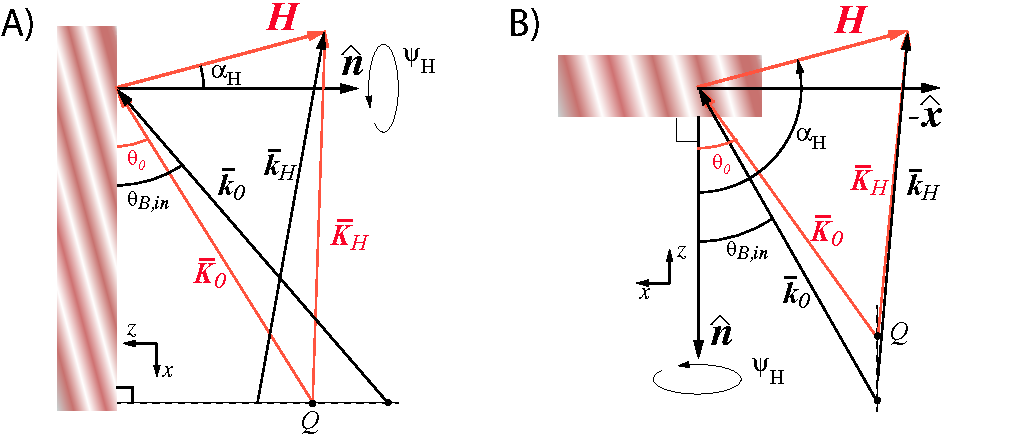
\includegraphics[width=5in]{crystal-diffraction.pdf}
  \caption[Reference trajectory reciprocal space diagram for crystal diffraction.]
{Reference trajectory reciprocal space diagram for for A) Bragg diffraction and B) Laue
diffraction. The bar over the vectors indicates that they refer to the reference trajectory. The
$x$-$z$ coordinates shown are the element surface coordinates. All points in the diagram are in the
plane of the paper except for the tip of $\bfH$.  $\bfKbar_{0}$, and $\bfKbar_{H}$ are the wave
vectors inside the crystal and $\bfkbar_{0}$ and $\bfkbar_{H}$ are the wave vectors outside the
crystal. The reference photon traveling along the reference trajectory has $\bfKbar_0$ and
$\bfKbar_H$ originating at the $Q$ point. For Laue diffraction, the crystal faces are assumed
parallel.  For Bragg diffraction the crystal normal is in the $-\bfhat x$ direction while for Laue
diffraction the crystal normal is in the $-\bfhat z$ direction
  }
  \label{f:crystal.diffraction}
\end{figure}

%-------------------------------------------------------------------------
%-------------------------------------------------------------------------
\section{Crystal Element Tracking}
\label{s:crystal.tracking}

\textit{\large [Crystal tracking developed by Jing Yee Chee, Ken Finkelstein, and David Sagan]}

Crystal diffraction is modeled using dynamical diffraction theory. The notation here follows
Batterman and Cole\cite{b:batterman}.  The problem can be divided up into two parts. First the
reference trajectory must be calculated. This means calculating the incoming grazing angle
$\theta_{B,in}$ and outgoing grazing angle $\theta_{B,out}$ as well as calculating the
transformations between the various coordinate systems. This is done in \sref{s:crystal.ref},
\sref{s:crystal.trans}, and \sref{s:laue.ref}.  The second part is the actual tracking of the photon
and this is covered in \sref{s:bragg.track} and \sref{s:coherent.laue}
%% and \sref{s:incoherent.laue}.

%-------------------------------------------------------------------------
\subsection{Calculation of Entrance and Exit Bragg Angles}
\label{s:crystal.ref}

\fig{f:crystal.diffraction} shows the geometry of the problem. The bar over the vectors indicates
that they refer to the reference trajectory. The reference trajectory is calculated such that the
reference photon will be in the center of the Darwin curve. That is, the internal wave vectors
$\bfKbar_0$ and $\bfKbar_H$ originate from the $Q$ point (See \cite{b:batterman} Figs.~8 and 29).

The external wave vectors $\bf k_0$, and $\bf k_H$ and the internal wave vectors
have magnitude
\begin{align}
  |\bf k_0| &= |\bf k_H| = \frac{1}{\lambda} 
  \label{kk1l1} \\
  |\bfKbar_0| &= |\bfKbar_H| = \frac{1 - \delta}{\lambda}
  \label{kk1l2}
\end{align}
where $\lambda$ is the wavelength, and $\delta$ is
\begin{equation}
  \delta = \frac{\lambda^2 r_e}{2 \, \pi \, V} \, F_0' = \frac{\Gamma}{2} \, F_0'
  = \frac{1}{2} \, \Gamma \, F_0'
\end{equation}
with $r_e$ being the classical electron radius, $V$ the unit cell volume, and $F_0'$ is the real
part of the $F_0$ structure factor.

In element surface coordinates (which will be the coordinate system used henceforth), $\bfkbar_0$
lies in the $x$-$z$ plane. $\bfKbar_0$ is related to $\bfkbar_0$ via Batterman Eq.~(25)
\begin{equation}
  \bfK_0 = \bfk_0 + q_0 \, \bfhat n
  \label{kkqn1}
\end{equation}
where the value of $q_0$ is to be determined. Here, and in equations below, if the equation is true
in general, and not just for the reference trajectory, the bar superscript is dropped.

Since $\bfhat n$ is in the $-\bfhat x$ direction, $\bfKbar_0$ is also in the $x$-$z$ plane. Thus
$\bfkbar_0$ and $\bfKbar_0$ can be written in the form
\begin{alignat}{3}
  \bfkbar_0 &= \frac{1}{\lambda} \, 
    \begin{pmatrix}
    -\cos\theta_{B,in} \\
    0 \\
    \sin\theta_{B,in}
    \end{pmatrix}
  \; , & \qquad
  \bfKbar_0 &= \frac{1 - \delta}{\lambda} \, 
    \begin{pmatrix}
    -\cos\theta_0 \\
    0 \\
    \sin\theta_0
    \end{pmatrix}
  & \qquad &\text{[Bragg]} \CRNO
  \bfkbar_0 &= \frac{1}{\lambda} \, 
    \begin{pmatrix}
    \sin\theta_{B,in} \\
    0 \\
    \cos\theta_{B,in}
    \end{pmatrix}
  \; , & \qquad
  \bfKbar_0 &= \frac{1 - \delta}{\lambda} \, 
    \begin{pmatrix}
    \sin\theta_0 \\
    0 \\
    \cos\theta_0
    \end{pmatrix}
  &\qquad & \text{[Laue]} 
  \label{k1lst}
\end{alignat}
Where, as shown in \fig{f:crystal.diffraction}, $\theta_{B,in}$, and
$\theta_0$ are the angles of $\bfkbar_0$ and $\bfKbar_0$ with respect
to the $x$-axis for Bragg reflections and with respect to the $z$-axis
for Laue reflection. 

$\alpha_H$ (\vn{alpha_angle}) is the angle that $\bfH$ makes with
respect to the $-\bfhat z$ axis and $\psi_H$ (\vn{psi_angle}) is the
rotation of $\bfH$ around the $-\bfhat z$ axis such that for $\psi_H =
0$, $\bfH$ is in the $x$-$z$ plane and oriented as shown in
\fig{f:crystal.diffraction}. Thus
\begin{equation}
  \bfH 
  \equiv \frac{1}{d} \, \bfhat{H} 
  = \frac{1}{d}
    \begin{pmatrix} 
       -\sin \alpha_H \, \cos \psi_H \\ \sin \alpha_H \, \sin \psi_H \\ -\cos \alpha_H
    \end{pmatrix}
  \label{h1daa}
\end{equation}
where $\bfhat{H}$ is $\bfH$ normalized to 1. $\alpha_H$ is determined
via the setting of \vn{b_param} and via \Eq{batat}.

The vectors $\bfK_0$ and $\bfH$ must add up to the reciprocal lattice vector $\bfK_H$
\begin{equation}
  \bfK_H = \bfK_0 + \bfH
  \label{kkh}
\end{equation}
Taking the length of both sides of this equation and using
\Eqs{kk1l2}, \eq{k1lst}, and \eq{h1daa} gives for
$\theta_0$
\begin{equation}
  \sin \theta_0 = 
  \begin{dcases}
    \dsfrac{-\beta \, \what{H}_z - \what{H}_x \, \sqrt{\what{H}_x^2 + \what{H}_z^2 - \beta^2}}
    {\what{H}_x^2 + \what{H}_z^2} & \vn{Bragg} \\
    \dsfrac{-\beta \, \what{H}_x + \what{H}_z \, \sqrt{\what{H}_x^2 + \what{H}_z^2 - \beta^2}}
    {\what{H}_x^2 + \what{H}_z^2} & \vn{Laue}
  \end{dcases}
\end{equation}
where
\begin{equation}
  \beta \equiv \frac{\lambda}{2 \, d \, (1 - \delta)}
\end{equation}
Once $\theta_0$ has been calculated, $\theta_{B,in}$ can be calculated from \Eq{kkqn1}
\begin{align}
  \cos\theta_{B,in} &= (1 - \delta) \, \cos\theta_0 \quad [\text{Bragg}] \\
  \sin\theta_{B,in} &= (1 - \delta) \, \sin\theta_0 \quad [\text{Laue}] 
\end{align}

The outgoing reference wave vector $k_H$ is computed using the equation
\begin{equation}
  \bfK_H = \bfk_H + q_H \, \bfhat n
  \label{kkqn2}
\end{equation}
Using this with \Eqs{h1daa} and \eq{kkh} gives
\begin{align}
  \kbar_{H,x} &= \Kbar_{H,z} = \frac{1}{d} \, \what{H}_x + \kbar_{0,x} \CRNO
  \kbar_{H,y} &= \Kbar_{H,y} = \frac{1}{d} \, \what{H}_y 
  \label{k1dapl} \\
  \kbar_{H,z} &= \sqrt{\frac{1}{\lambda^2} - \kbar_{H,x}^2 - \kbar_{H,y}^2} \nonumber
\end{align}

The total bending angle of the reference trajectory is then
\begin{equation}
  \theta_{bend} = \tan^{-1} 
  \left( \frac{ | \bfkbar_0 \cross \bfkbar_H | }{\bfkbar_0 \dotproduct \bfkbar_H} \right) 
\end{equation}
The outgoing Bragg angle $\theta_{B,out}$ is then {\em defined} to be
the difference between the total bend angle and the entrance Bragg angle.
\begin{equation}
  \theta_{B,out} \equiv \theta_{bend} - \theta_{B,in}
\end{equation}

%-------------------------------------------------------------------------
\subsection{Crystal Coordinate Transformations}
\label{s:crystal.trans}

There are four transformations needed between coordinates
denoted by $\Bf\Sigma_1$, $\Bf\Sigma_2$, $\Bf\Sigma_3$, and $\Bf\Sigma_4$
\begin{example}
  \(\Bf\Sigma_1\)  Transform from laboratory entrance to element entrance coordinates.  
  \(\Bf\Sigma_2\)  Transform from element entrance to surface coordinates.  
  \(\Bf\Sigma_3\)  Transform from surface to element exit coordinates.  
  \(\Bf\Sigma_4\)  Transform from element exit to laboratory exit coordinates.  
\end{example}
The total transformation is just the map represented by $\bfS$ and
$\bfV$ of \Eqs{vwlv} and \eq{wws}
\begin{equation}
  [\bfS, \bfV] = \Bf\Sigma_4 \, \Bf\Sigma_3 \, \Bf\Sigma_2 \, \Bf\Sigma_1
\end{equation}

\index{tilt_corr}\index{crystal!tilt correction}
The transformation $\Bf\Sigma_1$ is given in
\sref{s:crystal.trans.le} and the transformation $\Bf\Sigma_4$ is
given in \sref{s:crystal.trans.el}. In general, the transformation
$\Bf\Sigma_1$ needs a ``tilt correction'' (\Eq{tttt}), as explained
below, when $\psi_H$ is nonzero.  [The exception is when the
\vn{undiffracted} or \vn{forward_diffracted} beam is tracked with Laue
geometry. In these cases, no tilt correction is needed.] Since this
tilt correction is independent of any misalignments, the tilt
correction calculation proceeds assuming here that there are no
misalignments. The finite $\bfV$ due to the finite crystal thickness
in Laue diffraction will also be ignored for the moment.

Without misalignments, and with $\psi_H$ zero, the transformation
$\Bf\Sigma_1$ is, as it is for every other type of element,
just the unit matrix. 
\begin{equation}
  \Bf\Sigma_1 = \bfI
\end{equation}
That is, the two coordinate systems are
identical. Furthermore, the transformation $\Bf\Sigma_2$ from element
entrance coordinates to surface coordinates is a rotation around the $y$
axis
\begin{align}
  \Bf\Sigma_2 &= \bfR_y(\theta_{B,in}) \equiv \begin{pmatrix}
     \cos\theta_{B,in} & 0 & \sin\theta_{B,in} \\
     0                 & 1 & 0                 \\
    -\sin\theta_{B,in} & 0 & \cos\theta_{B,in} \\
  \end{pmatrix}
  \qquad &\text{[Laue]}
  \label{mt0t010} \\
  &= \bfR_y(\theta_{B,in} - \frac{\pi}{2})
  \qquad &\text{[Bragg]} \nonumber
\end{align}
The transformation from element surface coordinates to element exit
coordinates, $\Bf\Sigma_3$, is another rotation around the $y$ axis 
\begin{align}
  \Bf\Sigma_3 &= \bfR_y(\theta_{B,out})
  \qquad &\text{[Laue]} \\
  &= \bfR_y(\theta_{B,out} + \frac{\pi}{2})
  \qquad &\text{[Bragg]} \nonumber
\end{align}
and the transformation from element exit coordinates
to laboratory exit coordinates, $\Bf\Sigma_{out}$ is the unity matrix
\begin{equation}
  \Bf\Sigma_4 = \bfI
\end{equation}
Thus, the combined transformation $\bfS$ from laboratory entrance to
laboratory exit coordinates is a rotation around the $y$ axis of
$\theta_{B,in}+\theta_{B,out}$ as explained in section
\sref{s:global}
\begin{equation}
  \bfS = \Bf\Sigma_4 \, \Bf\Sigma_3 \, \Bf\Sigma_2 \, \Bf\Sigma_1 
  = \bfR_y(\theta_{B,in}+\theta_{B,out})
\end{equation}

\index{ref_tilt}\index{psi_angle}
When $\psi_H$ is non-zero, the situation is complicated since, if
$\bfS$ as calculated above is used, the vector $\bfkbar_H$ would be
bent out of the $x$-$z$ plane even though it has been assumed that the
\vn{ref_tilt} $\theta_t$ is zero. But $\bfkbar_H$ points in the same
direction as the $z$ axis of the outgoing reference
trajectory. Furthermore, by {\em definition}, the reference trajectory
has the form given by \Eq{ustt} with the $\bfR_{z}(\theta_t)$ matrix
depending only upon the \vn{ref_tilt} parameter (which is here taken
to be zero). To satisfy \Eq{ustt}, the crystal must be reoriented to
keep the $\bfk_H$ vector in the $x$-$z$ plane of the laboratory
entrance coordinates.  The reorientation is done by rotating the
crystal about the laboratory entrance $\Bf z$ axis by an amount
$\theta_{corr}$ (\vn{tilt_corr}).

With this tilt correction the transformation $\Bf\Sigma_1$ is a
rotation about the $z$ axis
\begin{equation}
  \Bf\Sigma_1 = 
  \begin{pmatrix}
    \cos\theta_{corr} & -\sin\theta_{corr} & 0 \\
    \sin\theta_{corr} &  \cos\theta_{corr} & 0 \\
    0                 &  0                 & 1                
  \end{pmatrix}
\end{equation}
To calculate a value for $\theta_{corr}$, note that
the transformation $\Bf\Sigma_2$ from element entrance coordinates to element surface
coordinates is not affected by a finite $\psi_H$ and so \Eq{mt0t010}
is unmodified. The $\bfk_H$ vector, expressed in laboratory entrance
coordinates, is $\Bf\Sigma_1^{-1} \, \Bf\Sigma_2^{-1} \, \bfk_H$ where the
components of $\bfk_H$ are given by \Eq{k1dapl}. To
satisfy \Eq{ustt}, this vector must have zero $y$ component
\begin{equation}
  \left( \Bf\Sigma_1^{-1} \, \Bf\Sigma_2^{-1} \, \bfk_H \right) \dotproduct
  \begin{pmatrix} 0 \\ 1 \\ 0 \end{pmatrix}
  = 0
\end{equation}
Solving gives
\begin{equation}
  \theta_{corr} = \tan^{-1} 
  \frac{k_{H,y}}{k_{H,z} \, \sin\theta_{B,in} - k_{H,x} \, \cos\theta_{B,in}}
\end{equation}
The transformation $\Bf\Sigma_3$ from element surface coordinates to
element exit coordinates is now obtained by requiring that the total
transformation from laboratory entrance to laboratory exit coordinates
be the $\bfR_{y}(-\alpha_b)$ matrix given in \Eq{ustt}
\begin{equation}
  \Bf\Sigma_3 \, \Bf\Sigma_2 \, \Bf\Sigma_1 = 
  \begin{pmatrix}
    \cos\theta_{bend} & 0 & -\sin\theta_{bend} \\
    0          & 1 & 0           \\
    \sin\theta_{bend} & 0 & \cos\theta_{bend}
  \end{pmatrix}
\end{equation}
In the above equation, the transformation $\Bf\Sigma_4$ has been
dropped since it is the unit matrix independent of $\psi_H$.

For Laue diffraction when the non-diffracted beam is tracked, the exit
coordinate system corresponds to the entrance coordinate system. That
is, $\bfV$ is the unit matrix. In this case, there is no tilt
correction and $\Bf\Sigma_3 = \bfR_y(-\theta_{B,in})$ is just the
inverse of $\Bf\Sigma_2$.

%-------------------------------------------------------------------------

\begin{figure}
\centering
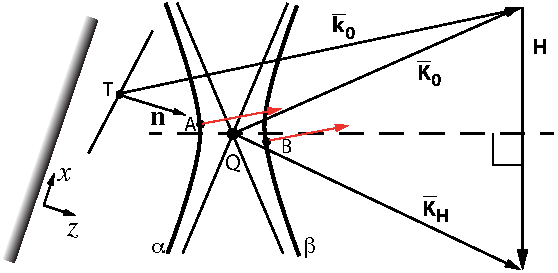
\includegraphics[width=4in]{crystal-energy.pdf}
  \caption[Reference energy flow for Laue diffraction]{
Energy flow used to determine the reference orbit for Laue diffraction.
  }
\label{f:crystal.energy}
\end{figure}

%-------------------------------------------------------------------------
\subsection{Laue Reference Orbit}
\label{s:laue.ref}

For Laue diffraction, with the reference orbit following the \vn{undiffracted} beam, the reference
orbit at the exit surface is just the extension of the reference orbit at the entrance
surface. Since the reference orbit's direction is $\bfkbar_0$.  the reference orbit displacement
vector $\bfL$ (cf.~\Eq{vwlv}) is given by
\begin{equation}
  \bfL = \frac{t^2}{d\bfkbar_0 \dotproduct \Bf t} \, d\bfkbar_0
  \qquad \text{[undiffracted]}
\end{equation}
where
\begin{equation}
  \Bf t = \begin{pmatrix}
    0 \\ 0 \\ t
  \end{pmatrix}
\end{equation}
with $t$ being the crystal thickness and the $z$-axis pointing into the crystal as illustrated in
\fig{f:crystal.energy}. The $\bfS$ rotation matrix (\Eq{wws}) for the undiffracted beam 
will be the unit matrix.

With the reference orbit following the \vn{forward_diffracted} or \vn{Bragg_diffracted} beam, the
displacement vector $\bfL$ follows the energy flow associated with the tie points labeled $A$ or $B$
in \fig{f:crystal.energy}. These tie points are defined by the intersection of the dispersion
surfaces and the vector $\Bf n$ originating from the point $T$ as shown in the figure.  The energy
flow is perpendicular to the dispersion surface and it can be shown that since, by construction,
$\Bf n$ goes through the $Q$ point, and since the dispersion surfaces are hyperboles, the energy
flows from $A$ and $B$ tie points are colinear. The direction of the energy flow is given by:
\begin{equation}
  \bfKbar_f = \xi_H \, \bfKbar_H + \xi_0 \, \bfKbar_0
\end{equation}
where $\xi_H$ and $\xi_0$ are given by \cite{b:batterman} Eq.~(18) (See section \sref{s:bragg.track} below).
$\bfL$ is thus
\begin{equation}
  \bfL = \frac{t^2}{\bfKbar_f \dotproduct \Bf t} \, \bfKbar_f
\end{equation}
At the exit surface, if the reference orbit is following the \vn{forward_diffracted} beam, the
orientation of the \vn{element exit} coordinates will be the same as the orientation of the
\vn{element entrance} coordinates. That is, $\bfS$ (\Eq{wws}) is the unit matrix.  If the reference
orbit is following the \vn{Bragg diffracted} beam, $\bfS$ is the same as for Bragg diffraction
\begin{equation}
  \bfS = 
  \begin{pmatrix}
    \cos\theta_{bend} & 0 & -\sin\theta_{bend} \\
    0                 & 1 & 0           \\
    \sin\theta_{bend} & 0 & \cos\theta_{bend}
  \end{pmatrix}
\end{equation}

%-------------------------------------------------------------------------
\subsection{Crystal Surface Reflection and Refraction}

%%%\begin{figure}[tb]
%%%  \centering
%%%  \includegraphics[width=5in]{crystal-surface-reflect.pdf}
%%%  \caption[Reflection from a crystal surface.]
%%%{Reflection from a crystal surface.}
%%%  \label{f:crystal.reflect}
%%%\end{figure}


There are corrections to the field amplitude and phase when a photon reflects or refracts from the
surface of a crystal. A plane wave is incident on a crystal surface with
\begin{equation}
  E = \what E_0 \, \exp(i \, \bfk_0 \, \bfr)
\end{equation}
An outgoing plane wave has a field
\begin{equation}
  E = \what E_1 \, \exp(i \, \bfk_1 \, \bfr)
\end{equation}
A simulation of this condition will start with a number of photons with wave vector $\bfk_0$ and
electric field $E_0$. After reflecting from the surface, the photons will have wave vector
$\bfk_1$. Now imagine a set of $N$ photons that flow through an planar area $dA_0$, perpendicular to
the incoming beam, before being reflected from the surface.

Since the electric field is $\what E_0$, when tracking incoherent photons
\begin{equation}
  \what E_0^2 = \frac{\alpha_p \, E_0^2 \, N}{dA_0}
\end{equation}
where $\alpha_p$ is the simulation constant (cf.~\Eq{panda1}. 
After the photons are reflected they will have some field $E_1$ and thus
\begin{equation}
  \what E_1^2 = \frac{\alpha_p \, E_1^2 \, N}{dA_1}
\end{equation}
Where $dA_1$ is the area that the photons flow through which is related
to $dA_0$ via
\begin{equation}
  \frac{dA_1}{dA_0} = \frac{\bfk_1 \dotproduct \bfz}{\bfk_0 \dotproduct \bfz} \equiv |b|
\end{equation}
Combining the above three equations, the change in field for a photon
as it reflects from the surface is
\begin{equation}
  \frac{E_1}{E_0} = \frac{\what E_1}{\what E_0} \, \sqrt{|b|} 
  \qquad \text{Incoherent}
\end{equation}

For coherent photon tracking the electric field at $dA_0$ is
\begin{equation}
  \what E_0 = \frac{\alpha_p \, E_0 \, N}{dA_0}
\end{equation}
After the photons are reflected they will have some field $E_1$ and thus
\begin{equation}
  \what E_1 = \frac{\alpha_p \, E_1 \, N}{dA_1}
\end{equation}
Combining these equations the change in field for a photon
as it reflects from the surface is
\begin{equation}
  \frac{E_1}{E_0} = \frac{\what E_1}{\what E_0} \, |b| 
  \qquad \text{Coherent}
\end{equation}

Additionally, for coherent tracking, all photons in a plane wave must
have the same phase when passing through an area transverse to the
wave. Thus the two photons labeled $a$ and $b$ in
\fig{f:crystal.reflect} must have the same phase advance in going from
$dA_0$ to $dA_1$. The difference in the phase advance for photon $b$
relative to $a$ from $dA_0$ to the surface is $\bfk_0 \dotproduct \bfr$
where $\bfr$ is the vector between where photon $b$ hits the surface
relative to photon $a$. Similarly, the difference in the phase advance
for photon $b$ relative to $a$ from the surface to $dA_0$ is $-\bfk_1
\dotproduct \bfr$. Since the total phase advance for both photons is the
same from $dA_0$ to $dA_1$ the phase shift $d\phi_b$ of photon $b$ as
it is reflected from the surface relative to the phase shift $d\phi_a$
is
\begin{equation}
  d\phi_b = d\phi_a - (\bfk_1 - \bfk_0) \dotproduct \bfr
  \label{dpbdpa}
\end{equation}

This shift in the reflection phase can be related to the lattice
diffraction planes. The wave vector difference can be written
\begin{equation}
  \bfk_1 - \bfk_0 = \bfH + q \, \bfhat n
  \label{k1k0}
\end{equation}
where $\bfhat n$ is perpendicular to the surface. Combining
\Eqs{dpbdpa} and \eq{k1k0} and since $\bfr$ is in
the plane of the surface
\begin{equation}
  d\phi_b = d\phi_a - \bfH \dotproduct \bfr
\end{equation}
This shows that the reflection shift has the same periodicity as the
pattern of the lattice planes at the surface of the crystal. Notice
that for a mirror, where one point on the surface is the same as any
other, $d\phi_b$ must be equal to $d\phi_a$. Using this in \Eq{dpbdpa}
gives 
\begin{equation}
  \bfk_1 \dotproduct \bfr = \bfk_0 \dotproduct \bfr
\end{equation}
and since $|\bfk_1| = |\bfk_0|$ this proves that the angle of
incidence is equal to the angle of reflection for a mirror.

In practice, the registration of the surface planes with respect to
the surface is not specified in a simulation. Thus the reflection
phase shift can only be calculated up to a constant offset. 

%-------------------------------------------------------------------------
\subsection{Bragg Crystal Tracking}
\label{s:bragg.track}

The starting photon coordinates are specified in the laboratory entrance coordinates. The
transformation from laboratory entrance coordinates to element entrance coordinates $\bftilde k_0$
is given in \sref{s:photon.lab.ele}. The transformation to element surface coordinates $\bfk_0$ is
\begin{equation}
  \bfk_0 =  \Bf\Sigma_2 \, \bftilde k_0
\end{equation}
with $\Bf\Sigma_2$ given by \Eq{mt0t010}.
The outgoing wave vector $\bfk_H$ is related to $\bfk_0$ via
\begin{equation}
  \bfk_H =  \bfk_0 + \bfH + q_t \, \bfhat n
\end{equation}
where $q_t$ is determined by using \Eqs{k1lst} and \eq{h1daa} in \Eq{kk1l1}
\begin{align}
  k_{H,x} &= k_{0,x} + H_x \nonumber \CRNO
  k_{H,y} &= k_{0,y} + H_y \\
  k_{H,z} &= \sqrt{\lambda^2 - k_{H,x}^2 - k_{H,y}^2} \nonumber
\end{align}

To compute the field amplitude of the outgoing photon, the equation to be solved is
(\cite{b:batterman} Eq.~(21))
\begin{equation}
  \xi_0 \, \xi_H = \frac{1}{4} \, k^2 \, P^2 \, \Gamma^2 \, F_H \, F_{\bar H}
  \label{xx14}
\end{equation}
where $\xi_0$ and $\xi_H$ are given by \cite{b:batterman} Eq.~(18) and $P$ is the polarization
factor
\begin{equation}
  P = 
  \begin{cases}
    1               & \sigma \text{ polarization state} \\
    \cos 2\theta_g  & \pi \text{ polarization state}
  \end{cases}
\end{equation}
$2\theta_g$ is the angle between $\bfK_0$ and $\bfK_H$ which is well
approximated by $\theta_{B,in} + \theta_{B,out}$.

The solution to \Eq{xx14} is (\cite{b:batterman} Eq.~(31))
\begin{align}
  \xi_0 &= \frac{1}{2} \, k \, |P| \, \Gamma \, [F_H \, F_{\bar H}]^{1/2} \, 
    |b|^{1/2} \, [\eta \pm (\eta^2 + \sign(b))^{1/2}] \CRNO
  \xi_H &= \frac{1}{2} \, k \, |P| \, \Gamma \, [F_H \, F_{\bar H}]^{1/2} \, 
    \frac{1}{|b|^{1/2} \, [\eta \pm (\eta^2 + \sign(b))^{1/2}]}
\end{align}
where the $+$ part of $\pm$ is for the $\alpha$ branch and the $-$ part of $\pm$ is for the $\beta$
branch and $\sign$ is the sign function
\begin{equation}
  \sign(b) \equiv \begin{cases} 1 & b > 0 \\ -1 & b < 0 \end{cases}
\end{equation}
and $\eta$ is given by \cite{b:blasdell} Eq.~(5)
\begin{equation}
  \eta = \frac{-b \, a + \Gamma \, F_0 \, (1 - b)}{2 \, \Gamma \, |P| \, \sqrt{|b| \, F_H \, F_{\bar H}}}
\end{equation}
with the asymmetry factor $b$ for the photon being tracked being given by \cite{b:blasdell} Eq.~(3)
\begin{equation}
  b \equiv \frac{\bfhat n \dotproduct \bfhat k_0}{\bfhat n \dotproduct (\widehat{{\bfk_0 + \bfH}})}
\end{equation}
and the angular deviation variable $a$ is given by \cite{b:blasdell} Eq.~(4)
\begin{equation}
  a \equiv \frac{H^2 + 2 \, \bfk_0 \dotproduct \bfH}{k_0^2} 
  = -2 \, \Delta \theta \, \sin(2\theta_B)
\end{equation}
Once $\xi_0$ and $\xi_H$ are determined, the ratio of the incoming and outgoing fields for the
$\alpha$ or $\beta$ branches can be computed via (\cite{b:batterman} Eq.~(24))
\begin{equation}
  r_E \equiv \frac{\bfE_H}{\bfE_0} 
  = \frac{- \, 2 \, \xi_0}{k \, P \, \Gamma \, F_{\bar H}} \,
  = \, \frac{- \, k \, P \, \Gamma \, F_H}{2 \, \xi_H} 
\end{equation}
where the $\alpha$ or $\beta$ subscript has been suppressed.  The total field which is the sum of the
fields on the branches is computed using the boundary conditions
\begin{equation}
  \bfE_0 = \bfE_{0\alpha} + \bfE_{0\beta}, \qquad\qquad 
  0 = \bfE_{H\alpha} + \bfE_{H\beta}
\end{equation}
Using the above two equations gives
\begin{align}
  \bfE_{0\alpha} &= \bfE_0 \, \frac{r_{E\beta}}{r_{E\beta} - r_{E\alpha}} \qquad\qquad
  \bfE_{H\alpha}  = \bfE_0 \, \frac{r_{E\alpha} \, r_{E\beta}}{r_{E\beta} - r_{E\alpha}} \CRNO
  \bfE_{0\beta} &= -\bfE_0 \, \frac{r_{E\alpha}}{r_{E\beta} - r_{E\alpha}} \qquad\qquad
  \bfE_{H\beta}  = -\bfE_0 \, \frac{r_{E\alpha} \, r_{E\beta}}{r_{E\beta} - r_{E\alpha}} 
\end{align}

As can be seen from Battermann and Cole Figs.~(8) and (29), the $\alpha$ tie point is excited and
the $\beta$ tie point is not if $\xi_{0\alpha} < \xi_{0\beta}$ and vice versa. Since only one tie
point is excited, The external field ratio is equal to the internal field ratio
\begin{equation}
  \frac{E_H^e}{E_0^i} = \frac{E_{Hj}}{E_{0j}}
\end{equation}
where $j$ is $\alpha$ or $\beta$ as appropriate.

%-------------------------------------------------------------------------
\subsection{Coherent Laue Crystal Tracking}
\label{s:coherent.laue}

Laue diffraction has two interior wave fields (branches), labeled $\alpha$ and $\beta$,
corresponding to the two tie points that are excited on the two dispersion surfaces. For coherent
tracking, a photon has some probability to be channeled to follow the $\alpha$ or $\beta$
branch. The electric field ratios $\what E_\alpha$ and $\what E_\beta$ (cf.~\Eq{rpss2}) are taken to
be equal to each other. With this choice, the probabilities $P_\alpha$ and $P_\beta$ for being
channeled to the $\alpha$ or $\beta$ branches are such that a branch with a greater intensity will
have a greater number of photons channeled down it.

When a crystal's \vn{ref_orbit_follows} parameter is set to \vn{bragg_diffracted}, The branching
probabilities are
\begin{equation}
  P_\alpha = \frac{|E_{H\alpha}|}{|E_{H\alpha}| + |E_{H\beta}|} , \qquad
  P_\beta = \frac{|E_{H\beta}|}{|E_{H\alpha}| + |E_{H\beta}|} , \qquad
  \what E_{H\alpha} = \what E_{H\beta}  = \frac{|E_{H\alpha}| + |E_{H\beta}|}{|E_0^i|}
\end{equation}
where (see Battermann and Cole\cite{b:batterman} Eqs~(42)), 
\begin{align}
  E_{H\alpha} &= -E_0^i \, \dsfrac{|b|^{1/2}}{2 \, \cosh v} \, 
    \frac{|P|}{P} \, 
    \frac{[F_H \, F_\Hbar]^{1/2}}{F_H} \, 
    \exp({-2 \, \pi \, i \, \bfK'_{H\alpha} \dotproduct \bfr_\alpha}) \,
    \exp({-2 \, \pi \, \bfK''_{H\alpha} \dotproduct \bfr_\alpha}) \CRNO
  E_{H\beta} &= E_0^i \, \dsfrac{|b|^{1/2}}{2 \, \cosh v} \, 
    \frac{|P|}{P} \, 
    \frac{[F_H \, F_\Hbar]^{1/2}}{F_H} \, 
    \exp({-2 \, \pi \, i \, \bfK'_{H\beta} \dotproduct \bfr_\beta}) \,
    \exp({-2 \, \pi \, \bfK''_{H\beta} \dotproduct \bfr_\beta})
\end{align}
where $\bfr_\alpha$ and $\bfr_\beta$ are the vectors from the entrance surface to the exit surface
for the $\alpha$ and $\beta$ wave fields
\begin{equation}
  \bfr_\alpha = \frac{t^2}{\bfS_\alpha \dotproduct \Bf t} \, \bfS_\alpha , \qquad
  \bfr_\beta = \frac{t^2}{\bfS_\beta \dotproduct \Bf t} \, \bfS_\beta
\end{equation}
with
\begin{align}
  \bfS_\alpha &= e^{-2 \, v} \, \Bf s_0 + \left| b \, \frac{F_H \, F_\Hbar}{F_H^2} \right| \, \Bf s_H \CRNO
  \bfS_\beta &= e^{2 \, v} \, \Bf s_0 + \left| b \, \frac{F_H \, F_\Hbar}{F_H^2} \right| \, \Bf s_H 
\end{align}
The phase shift of the electric field is obtained from the phase of $E_{H\alpha}$ if the photon is
channeled into the $\alpha$ branch and $E_{H\beta}$ if the photon is channeled into the $\beta$
branch.

When a crystal's \vn{ref_orbit_follows} parameter is set to \vn{forward_diffracted} or
\vn{undiffracted}, the algorithm is similar to the \vn{bragg_diffracted} case except $E_{0\alpha}$
and $E_{0\beta}$ are used in place of $E_{H\alpha}$ and $E_{H\beta}$ with
\begin{align}
  E_{0\alpha} &= E_0^i \, \dsfrac{e^{-v}}{2 \, \cosh v} \, 
    \exp({-2 \, \pi \, i \, \bfK'_{0\alpha} \dotproduct \bfr_\alpha}) \,
    \exp({-2 \, \pi \, \bfK''_{0\alpha} \dotproduct \bfr_\alpha}) \CRNO
  E_{0\beta} &= E_0^i \, \dsfrac{e^{-v}}{2 \, \cosh v} \, 
    \exp({-2 \, \pi \, i \, \bfK'_{0\beta} \dotproduct \bfr_\alpha}) \,
    \exp({-2 \, \pi \, \bfK''_{0\beta} \dotproduct \bfr_\beta})
\end{align}

Since a simulation photon has two polarization components, the above equations are used for one
polarization component and for the second polarization component the same branch is used as for the
first with an appropriately scaled $\what E$.

%-------------------------------------------------------------------------
%\subsection{Incoherent Laue Crystal Tracking}
%\label{s:incoherent.laue}
%
%Laue diffraction has two interior wave fields (branches), labeled $\alpha$ and $\beta$,
%corresponding to the two tie points that are excited on the two dispersion surfaces. For incoherent
%tracking it is assumed that these wave fields overlap at the exit surface (\cite{b:batterman}
%Eq.~(87)) and so add coherently. This is a good approximation if the crystal is very thin where the
%wave fields do not travel an appreciable spatial distance and is also a good approximation when the
%crystal is thick since the $\beta$ branch will be heavily attenuated. At intermediate thicknesses
%this approximation is good when a photon is near the Bragg angle since, in this case, the fields
%will be traveling in similar directions.
%
%Another approximation is that the path

%---------------------

%\begin{figure}[tb]
%  \centering
%  \includegraphics[width=5in]{mosaic-crystal.pdf}
%  \caption[Mosaic crystal Monte Carlo tracking.]{Mosaic crystal representation used for Monte Carlo tracking.}
%  \label{f:mosaic.crystal}
%\end{figure}
%
%%-------------------------------------------------------------------------
%\subsection{Mosaic Crystal Tracking}
%\label{s:mosaic.track}
%
%Tracking through a mosaic crystal tracking is illustrated in Figure~\ref{f:mosaic.crystal}. The
%\bmad algorithm is similar to the method presented by Alianelli et al. \cite{b:mosaic}. The mosaic
%crystal is idealized as a number of small perfect crystals, called crystallites, all of which have
%the same specified thickness $T_m$ (the \vn{mosaic_thickness} parameter of the crystal). The
%crystallites are all misoriented with angular probability distribution $W$ given by
%\begin{equation}
%  W(\theta, \phi) = \frac{1}{2 \, \pi \, \sigma_{in} \, \sigma_{out}} \exp \left(-
%  \frac{\theta^2}{2 \, \sigma_{in}^2} - \frac{\phi^2}{2 \, \sigma_{out}^2} \right)
%  \label{w12p}
%\end{equation}
%where $\theta$ is the misorientation angle in the diffraction plane and $\phi$ is the misorientation
%angle out of the diffraction plane. The sigmas, $\sigma_{in}$ and $\sigma_{out}$, correspond to the
%parameters of a crystal element (\sref{s:crystal}) \vn{mosaic_angle_rms_in_plane} and
%\vn{mosaic_angle_rms_out_plane} respectively.
%
%The crystalites are modeled to lie in layers of thickness $T_m$. For \vn{Laue} diffraction
%(\vn{b_param} > 0), the actual thickness $T_m$ used is adjusted so that there is an integer number
%of mosaic layers. That is
%\begin{equation}
%  T_m(\text{in simulation} = \frac{T}{\text{nint} (T/T_m)}
%\end{equation}
%where $T$ is the crystal thickness and \vn{nint} is the nearest integer function. 
%
%Tracking is done step-by-step with a photon either traversing or being reflected by a crystalite.
%Interference effects between crystallites are not taken into account so the tracking is incoherent
%(\sref{s:coher.incoher}).
%
%At the beginning of a step the photon is in between two layers and will be traveling towards one of
%these layers. A random number generator along with \Eq{w12p} is used to determine the misorientation
%of the crystallite that the photon is going through. Factoring this misorientation into account, the
%amplitude scattering $R$ and transmission $T$ probabilities are calculated using dynamical diffraction theory.
%
%A random number generator is used to determine if the photon is scattered or transmitted. If $P_T$ is the
%probability assigned for the probability of transmission, then
%\begin{equation}
%  r_T = 
%\end{equation}

%-------------------------------------------------------------------------
\section{X-ray Targeting}
\label{s:targeting}

X-rays can have a wide spread of trajectories resulting in many ``doomed'' photons that hit
apertures or miss the detector with only a small fraction of ``successful'' photons actually
contributing to the simulation results. The tracking of doomed photons can therefore result in an
appreciable lengthening of the simulation time. To get around this, \bmad can be setup to use what
is called ``targeting'' to greatly reduce the number of doomed photons generated.

Photons can be generated either at a source like a \vn{wiggler} element or at a place where
diffraction is simulated like at a \vn{diffraction_plate} element. To be able to do targeting, an
element with apertures defined must be present downstream from the generating element. The idea is
to only generate photons that are going in the general direction of the ``target'' which is the
space within the aperture.

A necessary restriction for targeting to work is that the photon must travel in a straight line
through all elements between the generating element and the element with the apertures. So, for
example, a \vn{crystal} element would not be allowed between the two two elements. A \vn{crystal}
element could be the aperture element as long as the aperture was defined before photons were
diffracted. That is, if the aperture was at the upstream end of the crystal or was defined with
respect to the \vn{crystal} surface.

The target is defined by the four corners of the aperture. In \vn{element} coordinates, the $(x, y,
z)$ values of the corners are:
\begin{example}
  (-x1_limit, -y1_limit, z_lim)
  (-x1_limit,  y2_limit, z_lim)
  ( x2_limit, -y1_limit, z_lim)
  ( x2_limit,  y2_limit, z_lim)
\end{example}
where \vn{x1_limit}, etc. are the aperture limits (\sref{s:limit}) and \vn{z_lim} will be zero
except if the element's \vn{aperture_at} parameter is set to \vn{entrance_end} in which case
\vn{z_lim} will be set to \vn{-L} where \vn{L} is the length of the element.

If the aperture is associated with a curved surface (for example with a \vn{crystal} element), four
extra corner points are also used to take into account that the aperture is not planar. These extra
points have $(x, y, z)$ values in \vn{element} coordinates of
\begin{example}
  (-x1_limit, -y1_limit, z_surface(-x1_limit, -y1_limit))
  (-x1_limit,  y2_limit, z_surface(-x1_limit,  y2_limit))
  ( x2_limit, -y1_limit, z_surface( x2_limit, -y1_limit))
  ( x2_limit,  y2_limit, z_surface( x2_limit,  y2_limit))
\end{example}
where \vn{z_surface(x,y)} is the $z$ value of the surface at the particular $(x, y)$ point being
used. Notice that in this case \vn{z_lim} is zero.

The coordinates of the four or eight corner points are converted from \vn{element} coordinates of
the aperture element to \vn{element} coordinates of the photon generating element. Additionally, the
approximate center of the aperture, which in \vn{element} coordinates of the aperture element is
$(0, 0, z_lim)$, is converted to \vn{element} coordinates of the photon generating element.

The above calculation only has to be done once at the beginning of a simulation.

When a photon is to be emitted from a given point $(x_{emit}, y_{emit}, z_{emit})$, the problem is
how to restrict the velocity vector $(\beta_x, \beta_y, \beta_z)$ (which is normalized to 1) to
minimize the number of doomed photons generated. The problem is solved by constructing a vector $\Bf
r$ for each corner point:
\begin{equation}
  \Bf r = (x_{lim}, y_{lim}, z_{lim}) - (x_{emit}, y_{emit}, z_{emit})
\end{equation} 
The direction of each $\Bf r$ is characterized in polar coordinates $(\phi, y)$ defined by
\begin{align}
  y &= \frac{r_y}{|r|} \CRNO
  \tan\phi &= \frac{r_x}{r_z} 
\end{align}
For now make the assumption that $r_z$ is positive and larger than $r_x$ and $r_y$ for all $\Bf r$.
Let $\phi_{max}$ and $\phi_{min}$ be the maximum and minimum $\phi$ values over all the $\Bf
r$. Similarly, let $y_{min}$ and $y_{max}$ be the minimum and maximum $y$ values over all the $\Bf
r$. The rectangle in $(\phi, y)$ space defined by these four min and max values almost covers the
projection of the aperture onto the unit sphere. There is a correction that must be made due to the
fact that a straight line of constant $y$ in $(x, y, z)$ space projects to a curved line when
projected onto $(\phi, y)$ space. Therefore a correction must be made to $y_{min}$ when $y_{min} <
0$:
\begin{equation}
  y_{min} \rightarrow 
  \frac{y_min}{\sqrt{(1 - y_{min}^2) \, \cos^2 (phi_{max} - \phi_{min})/2 + y_{min}^2}}
\end{equation}
with a similar correction for $y_{max}$ that must be made when $y_{max} > 0$.


The above prescription works as long as the projection of the aperture onto $(\phi, y)$ space does
not touch the branch cut at $\phi = \pi$ or cover the singular points $y = \pm 1$. Generally these
restrictions are fullfilled since $\Bf z$ is the direction of the reference orbit. If this is not
the case, a transformation can be made where rotation matrices are constructed to transform between
the \vn{element} coordinates of the emitting element and what are called \vn{target} coordinates
defined so that $\Bf r$ for the \vn{center} point has the form $(0, 0, |r|)$. The procedure for
calculating the photon velocity vector is now
  \begin{enumerate}
  \item
Rotate all the corner $\Bf r$ from \vn{element} to \vn{target} coordinates.
  \item
Calculate min and max values for $\phi$ and $y$.
  \item
Calculate the velocity vector such that the $(\phi, y)$ of this vector
falls within the min and max values in the last step.
  \item
Rotate the velocity vector back to \vn{element} coordinates.
  \end{enumerate}


\chapter{Simulation Modules}

In the \bmad ``ecosystem'', various modules have been developed to
simulate machine hardware. This chapter provides documentation.

%-----------------------------------------------------------------
\section{Tune Tracker Simulator}
\index{tune tracker simulation}

\textit{\large [Tune tracker simulation developed by Michael Ehrlichman]}

The digital tune tracker (dTT) is device for determining the
fractional tune of a storage ring and exciting resonant beam
oscillations.  In short, the dTT starts with a beam position monitor
(BPM) to detect the beam oscillations. The signal from the BPM is feed
into a phase-locked loop (PLL) circuit which oscillates at the
oscillation frequency the beam. A signal from the PLL is used to
modulate a kicker to keep the beam oscillating at the beam's
oscillation frequency. The tune tracker is capable of exciting both
betatron and synchrotron oscillations.

In general, a PLL is a control system for matching the frequency of a
VCO to some incoming periodic reference signal.  It does this by
adjusting the frequency of the VCO according to the phase difference
between the VCO output and the reference signal.  A general diagram of
a PLL is shown in \fig{f:PLL}.

  \begin{figure}[bt]
  \centering
  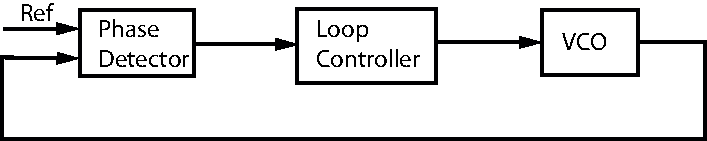
\includegraphics{PLL.pdf}
  \caption[General diagram of a phase lock loop.]{
General diagram of a phase lock loop. The loop adjusts the speed of a
VCO according to the phase difference between the VCO and an incoming
signal.}
  \label{f:PLL}
  \end{figure}

In \fig{f:PLL}, the phase detector compares the two incoming
signals, and outputs a signal that is proportional to the difference
in phase.  There are various ways to implement a phase detector.  The
tune tracker phase detector is a mixer followed by low-pass filter,
which will be discussed in more detail below.  The loop controller,
also known as a loop filter, is usually some combination of
(P)roportional, (I)ntegration, and (D)ifferentiation paths.  The loop
controller sums these paths, and the resulting signal is sent to the
VCO.  The output of the loop controller rises when the VCO is slower
than the reference, and drops when the VCO is faster.  The gains of
the three PID paths are adjusted to produce a control loop that is
stable and can efficiently lock onto the reference signal from some
incorrect initial frequency.  A real-world PLL also needs to track
perturbations to the reference frequency.

A diagram of the digital tune tracker is shown in
\fig{f:CdTT}.  This function takes in one new BPM measurement
per call, and returns a sinusoidal signal that has the same frequency
as the BPM signal.  The phase of the returned signal differs from the
phase of the BPM signal by $\phi_0$, the phase advance from position
at the BPM to position at the kicker on the next turn.

Comparing this diagram to the PLL in \fig{f:PLL}, the boxes
from {\it Subtract closed orbit offset} to the end of the {\it Low
Pass Filter} comprise the phase detector.  After the {\it Low Pass
Filter} to just before the {\it Gain Kvco} box comprises the loop
controller.  The {\it Gain Kvco} box comprises the VCO.  The feedback
loop consists of the update to $\omega$ that follows {\it Gain Kvco}.

\begin{sidewaysfigure}[tb]
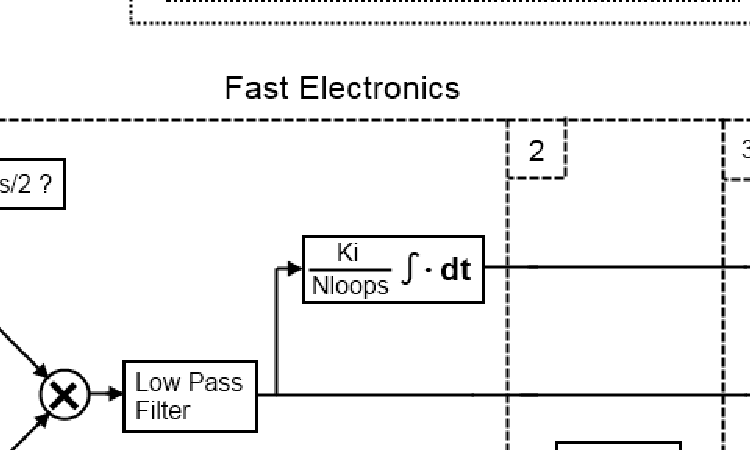
\includegraphics[width=\columnwidth]{TT-Flow.pdf}
\caption{
Flow chart of tune tracker module functions.}
\label{f:CdTT}
\end{sidewaysfigure}

\clearpage

\subsection{Tune Tracker Components.}
\begin{description}
\item[New BPM Meas.]  
This consists of one BPM measurement.  It is either horizontal or
vertical position at the BPM location.  It is assumed that each
measurement is separated by the same $\Delta t$, and that $\Delta t$
is an integer multiple of the ring period.

\item[Subtract closed orbit offset]  
Due to misalignments or the presence of wigglers, the closed orbit at
the BPM may be non-zero.  The closed orbit is subtracted from the
incoming data.  The closed orbit offset is a constant parameter set by
the user during initialization.

\item[Apply Gain G]  This block adjusts the incoming measurement such that,
\begin{equation*}
Meas.\ Out = \frac{Meas.\ In}{G}
\end{equation*}
The purpose of this block is to normalize the BPM measurements.  When
the tune tracker first starts, the amplitude of the beam oscillations
is small.  When the tune tracker is locked on, the amplitude of the
beam oscillations becomes large.  The set of loop controller gains
that allows the tune tracker to quickly lock onto the initially small
signal are not optimal when the beam oscillations are large.  This
normalization overcomes that problem, allowing for a set of loop
controller gains that are optimal both at start up and when
oscillations are large.

\item[Update Gain G]  This is a digital filter of the form,
\begin{equation*}
G = g_a \textrm{abs}\left(x\right) + \left(1-g_a\right)G\textrm{,}
\end{equation*}
which is a exponentially weighted moving average, or equivalently, a
low-pass filter.  $x$ is the incoming data point.  $g_a$ is a
hard coded time constant.  It is set so that $G$ equilibrates to the
rms beam size after about 10 periods.

\item[Fast Electronics]  
Fast electronics contains the components of the tune tracer that cycle
every few RF periods.  Whereas the rest of the tune tracker cycles
once per storage ring period, the fast electronics cycle every few RF
buckets.

\item[Prev Turn BPM Msmt]  Stores the previous turn's BPM measurement.

\item[Loop\# $\boldsymbol >$ $\boldsymbol N_{loops}/2$ ?]  
$N_{loops}$ is the number of times the fast electronics cycle every
storage ring period.  For the first half of these loops, the BPM
measurement from the previous turn is used.  For the last half, the
current BPM measurement is used.

\item[$\boldsymbol \sin\left(\psi\right)$]  
Sinusoid of the current modulator angle $\psi$.

\item[$\boldsymbol \psi$]  
Current modulator angle.  Updated at the end of every fast electronics loop.

\item[$\boldsymbol \times$ (times)]  
The BPM measurement and $\sin\left(\psi\right)$ are multiplied.  
Let the BPM signal be parameterized as $\cos\left(\omega_{beam}t\right)$, and 
write $\psi$ as $\omega_{vco}t$ so we have,
\begin{equation*}
\cos\left(\omega_{beam}t\right)\sin\left(\omega_{vco}t\right)\textrm{.}
\end{equation*}
A trig identity allows this to be written as,
\begin{equation*}
\frac{1}{2}\left(\sin\left(\left(\omega_{beam}+\omega_{vco}\right)t\right)-
\sin\left(\left(\omega_{beam}-\omega_{vco}\right)t\right)\right)\textrm{.}
\end{equation*}
If $\omega_{vco}$ is roughly $\omega_{beam}$, then the first $\sin$
term has roughly twice the beam frequency and the second term has a
very small frequency.  Therefore, passing the multiplied signal
through a low-pass filter removes the first term, leaving only the
second term.

In stable operation, $\omega_{vco}$ makes small amplitude oscillations
about $\omega_{beam}$.  In this case, the time integral of
$\left(\omega_{beam}-\omega_{vco}\right)t$ is small for all $t$, and a
small angle approximation for sine can be applied, and the output of
the low pass filter can be written as,
\begin{equation}
\left(\omega_{beam}-\omega_{vco}\right)t\textrm{,}
\end{equation}
which is proportional to the phase difference between the beam and the VCO.  Thus completes
the phase detector.

\item[$\boldsymbol{\frac{K_I}{N_{loops}}\int\cdot dt}$]  
This is the (I)ntegrated channel of the PID controller.  It integrates
the output of the phase detector, providing negative feedback.  If the
integrated phase is positive, the I channel slows the VCO down.  If
negative, it speeds the VCO up.  This channel is expected to
equilibrate to some non-zero value proportional to the difference
between the beam frequency and the VCO base frequency.

\item[Update $\boldsymbol{\psi}$] This increments the modulator phase according to,
\begin{equation}
\psi_{n+1}=\psi_n+\frac{T_{ring}}{N_{loops}}\omega_{vco}\textrm{.}
\end{equation}
In order to more accurately model things,
$\omega_{vco}$ is not updated within the fast electronics loop.

\item[Increment Loop\# by 1]  
Loop\# counts the number of times the fast electronics has been looped
through.

\item[If Loop\# $>$ $N_{loops}$, exit, else, loop]  
$N_{loops}$ is the number of times the fast electronics cycle per ring
period.

\item[Gain $\boldsymbol K_P$] 
This is the (P)roportional channel of the PID controller.  Is provides
negative feedback proportional to the output of the phase detector.
This channel responds faster than the integrated channel and so helps
the tune tracker track sudden changes in the frequency of the beam.
In practice, it also damps tune tracker oscillations.  If $K_P$ is too
small, the VCO may oscillate indefinitely around the fractional tune
of the beam.  See section~\sref{Tuning} below for more details.

\item[Gain $K_D$ $\times$ filtered derivative]  
This is the (D)ifferential channel of the PID controller.  Provides a
filtered first derivative of the output of the phase detector.  The
derivative is obtained a polynomial fitted to a history of the phase
detector output.  This channel can be used to smooth out the VCO
response and reduce overshoot.  See section~\sref{Tuning} below for
more details.

\item[$\boldsymbol +$ (sum)]  
This block sums the three output of the PID controller.

\item[Gain $K_{vco}$] 
This block represents the response of a voltage controlled oscillator.
The frequency of the output of a VCO is proportional to the voltage of
its input.  This block simply multiplies the output of the PID
controller by a constant.  This block updates the VCO frequency.

\item[$\boldsymbol{\sin\left(\psi+\psi_0\right)}$]  
Calculates kicker amplitude to be returned to the calling program.
This is the kick amplitude that should be used during the next turn.
$\psi_0$ is the phase advance from position at the BPM to position at
next turn's kicker.

\end{description}

\subsection{Tuning \label{Tuning}} Tuning the tune tracker consists of
adjusting the four gain parameters $K_P$, $K_I$, $K_D$, and $K_{vco}$.
The goal is to set the parameters such that the tune tracker quickly
locks onto the fractional tune of the beam, and settles quickly.  If
multiple tunes are being explored, then the size of the convergence
region is also important.  i.e.  The set of parameters should work for
a wide range of fractional tunes.  If jitter is being explored, then
the ability of the tune tracker to track a varying fractional tune is
also important.

A plot of the VCO speed during typical tune tracker operation is shown
in \fig{f:typ-tt}.  A tune tracker with a base period of 0.571
oscillations per ring period tracks a beam with a fractional tune of
0.5691.  Marked on this plot are 4 important features.  They are the
rise time, overshoot, settling rate, and precision.  The rise time is
how long it takes the tune tracker to approach the fractional tune of
the beam.  This is the location of the first peak after operation
begins.  The overshoot is the difference between the amplitude of the
first peak and the fractional tune.  The settling rate measures the
decay rate of the oscillations of the VCO about the fractional tune.
The precision is the noise in the VCO frequency.  The discrete nature
of the BPM measurements introduces noise at the phase detector stage.
The proportional channel adds this noise to the VCO frequency Shown in
Tab.~[\ref{t:pid-params}] is the effect increasing the PID controller
gains.

\begin{table}
\begin{tabular}{llllll} \toprule
Parameter&  Rise Time&        Overshoot&        Settling Rate&      Precision&  Stability Region\\ \midrule
$K_P$&      slight decrease&  decrease&         faster&             degrade&    shrink\\
$K_I$&      decrease&         increase&         slower&             no change&  shrink\\
$K_D$$^\textrm{see note}$&    slight increase&  slight decrease&  slightly faster&    degrade&    grow\\ \bottomrule
\end{tabular}
\caption[Effect on VCO response of increasing $K_P$, $K_I$, or $K_D$.]{
Effect on VCO response of increasing $K_P$, $K_I$, or $K_D$. 
{\it Note:} The effects of the derivative channel are theoritical and have not 
been verified extensively.}
\label{t:pid-params}
\end{table}

Stability region refers to the range of fractional tunes that the tune
tracker will converge to when starting from an initial tune in that
range.  In practice, if $K_P$ and $K_I$ are increased to optimize
response to a particular fractional tune, the stability region
will shrink.  e.g.  A large $K_P$ and $K_I$ could be found that very
quickly lock on to a fractional tune of 0.569, but are unstable for
0.622.  But note that a smaller $K_P$ and $K_I$ can be found that give
acceptible performance at 0.569, and also acceptible performance at
0.622 (and even 0.074).

\begin{figure}[tb]
\centering
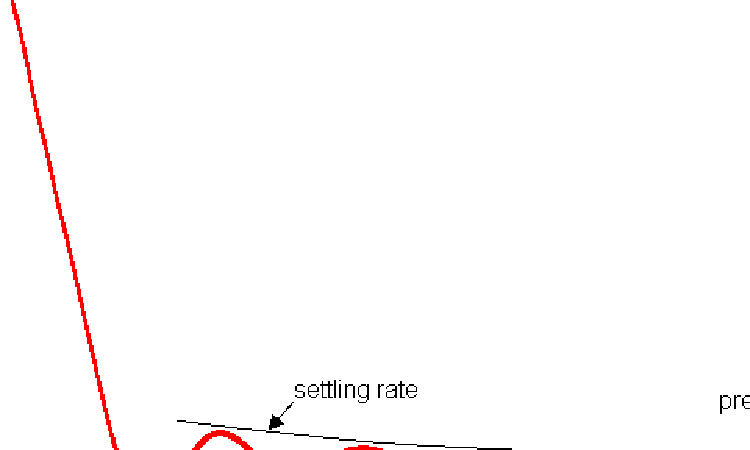
\includegraphics[scale=0.75]{vco-plot.pdf}
\caption[Plot of VCO response of typical tune tracker setup.]{
Plot of VCO response of typical tune tracker setup.  VCO base frequency is 0.571.
Beam fractional tune is 0.5691.}
\label{f:typ-tt}
\end{figure}

%----------------------------------------------------------------------

\subsection{Programmer Instructions}

This seciton contains instructions on how to implement the tune
tracker module and how to use the tune tracker driver program.  The
tune tracker is written as an object or class, and so supports
multiple instances.

After setting up the tune tracker in a program, it is best to first
verify that the tune tracker is efficiently locking onto the beam and
that the beam oscillations are indeed growing with time.  The tune
tracker should lock on after about 10,000 turns, and the beam
oscillations should reach equilibrium amplitude after about 10 damping
periods.

See the tune tracker section in the Physics chapter of this manual for
an example of how the VCO frequency should respond with time in a
successful implementation.  Guidelines for setting the gain parameters
are also located in the Physics chapter.

%-------------------------------------------------------------------------
\subsection{Tune Tracker Module}

The tune tracker module has four public functions.  They are,
\begin{alltt}
Function id = init_dTT(tt_param_struct)     !Constructor, creates new tune tracker 
                                            !instance, handles initialization.
                                            !Passed tt_param_struct, Returns id of 
                                            !created instance.
Function z = TT_update(bpm_msmt,id)         !Main function, passed one new BPM 
                                            !measurement and returns VCO modulator 
                                            !amplitude.
Subroutine dest_dTT(id)                     !Destructor, closes log files and 
                                            !deallocates memory.
                                            !Takes as argument id of instance 
                                            !to be destroyed.
Function z = get_dTT(name,id)               !Get function, name is either "wf", 
                                            !in which case the function returns 
                                            !the VCO frequency \(\omega0+\Delta\omega\), 
                                            !or "dw", in which case just \(\Delta\omega\)
                                            !is returned.
\end{alltt}

Pseudocode for a tune tracker implementation is below.
\begin{verbatim}
Populate tt_param_struct with tune tracker parameters.
id = init_dTT(tt_param_struct)
Loop over turns:
  Track once through the ring, obtain orbit.
  bpm_msmt = x or y at BPM location.
  z = TT_update(bpm_msmt,id)
  Adjust kicker amplitude (or cavity phase) according to z
dest_dTT(id)
\end{verbatim}

See {\tt tune\_tracker.f90} for the contents of {\tt tt\_param\_struct}.

If a horizontal or vertical tune tracker is to be implemented, the BPM
measrements should be the $x$ or $y$ coordinate at the BPM location,
and the kicks should be changes in $x'$ or $y'$ at the kicker
location.  If a longitudinal tune tracker is to be implemented the BPM
measurements should be the $x$ coordinate in a dispersive region, and
the kicks should be changes in phase at an RF cavity.  Similarly, if a
longitudinal tune tracker is being used in conjunction with a
horizontal tune tracker, the BPM of the horizontal tune tracker should
be placed in a region of low dispersion.  This will prevent the
horizontal tune tracker from inadvertantly locking onto the
synchrotron tune.

%-----------------------------------------------------------
\subsection{Tune Tracker Example Program}

An example program is located in {\tt
src/examples/tune\_tracker}. This program contains code for
implementing simultaneous horizontal, vertical, and longitudinal tune
trackers.

For most implementations of the tune tracker module, a good approach
would be to either use a modified version of the tune tracker example
program, or copy and paste code from the example program.  Keep in
mind that the example program implements multiple simultaneous tune
trackers.  An implementation of just one tune tracker would be much
simpler.

The example program performs the following steps.
\begin{enumerate}
\item 
Read in file which contains tune tracker parameters such as gains.
\item 
Parse lattice with {\tt twiss3} subroutines.  The {\tt twiss3} subroutines
are needed to obtain the longitudinal phase advance when implementing 
longitudinal tune trackers.
\item 
Check that the kick attribute of the kicker element is actually free.
\item 
Calculate phase advance from position at BPM to position at kicker.  Note that this 
is the phase of the kicker {\it on the next turn}.
\item 
Creates log files which record position at BPM and kicker, the VCO frequency,
and slope at the kicker.
\item
Loops over turns, passing BPM measurements to {\tt TT\_update} and
adjusting kicker amplitudes based on the returned value.  Note that it
will take the beam oscillations several damping times to equilibriate.
This often means tracking for several 10,000 turns.  Use of the save
state parameter may shorten simulation times in certain applications.
\item 
Calculates and FFT of the BPM data and records in log file. 
\end{enumerate}

Also located in {\tt src/examples/tune\_tracker} is an example .in
file that implements horizontal, vertical, and longitudinal tune
trackers.  The gains used in the .in file were selected for their
large convergence region.  More agressive tuning may lead to faster
lock on.  See the Physics section for details.

%----------------------------------------------------------------------------
\subsection{Save States}

If {\tt tt\_param\_struct\%useSaveState} is set to true, then the
destructor {\tt dest\_dTT} will save the tune tracker state variables
to a file called {\tt tt\_state.\#}.  Similarly, the constructor {\tt
init\_dTT} will set the state variables according to the save state
file.  The constructor will also return the beam coordinates to be
used at element zero of the ring.

Save states allow you to pick up where you left off, and not have to
wait for the beam oscillations to equilibriate.  For example, you
could have one program that tracks for 100,000 turns, allowing the
tune tracker to lock on and the beam excitation to equilibriate with
radiation damping.  The simulation writes a save state file which can
be used as a starting point for other simulations that perform studies
on the excited beam.

%-----------------------------------------------------------------
\section{Instrumental Measurements}
\label{s:meas.calc}
\index{measurement}

\bmad has the ability to simulate instrumental measurement errors
for orbit, dispersion, betatron phase, and coupling measurements.
The appropriate attributes are listed in \sref{s:meas.attrib} and
the conversion formulas are outlined below.

%-----------------------------------------------------------------
\subsection{Orbit Measurement}
\index{orbit!measurement}

For orbits, the relationship between measured position $(x, y)_{\text{meas}}$ and true position $(x,
y)_{true}$ is
\begin{equation}
  \begin{pmatrix}
    x \\ y
  \end{pmatrix}_{\! \text{meas}}
  =
  n_f \, 
  \begin{pmatrix}
    r_1 \\ r_2
  \end{pmatrix}
  +
  \bfM_m \, 
  \left[
  \begin{pmatrix}
    x \\ y
  \end{pmatrix}_{\! true}
  -
  \begin{pmatrix}
    x \\ y
  \end{pmatrix}_{\! 0}
  \right]
  \label{xynrr}
\end{equation}
where the Gaussian random numbers $r_1$ and $r_2$ are centered at zero and have unit width and the
factor $n_f$ represents the inherent noise in the measurement. In the above equation, $(x, y)_0$ 
represents a measurement offset and $\bfM_g$ is a ``gain'' matrix writen in the form
\begin{equation}
  \bfM_m
  =
  \begin{pmatrix}
     (1 + dg_x) \, \cos (\theta + \psi) & (1 + dg_x) \, \sin (\theta + \psi) \\
    -(1 + dg_y) \, \sin (\theta - \psi) & (1 + dg_y) \, \cos (\theta - \psi) 
  \end{pmatrix}
  \label{m1dg}
\end{equation}
Here $dg_x$ and $dg_y$ represent gain errors and the angles $\theta$ and $\psi$ are tilt and 
``crunch'' errors.

In the above equations, various quantities are writen as a difference between an ``error'' quantity
and a ``calibration'' quantity:
\begin{alignat}{1}
  x_0     &= x_{\text{off}} - x_{\text{calib}} \CRNO
  y_0     &= y_{\text{off}} - y_{\text{calib}} \CRNO
  \psi    &= \psi_{\text{err}}   - \psi_{\text{calib}} \CRNO
  \theta  &= \theta_{\text{err}} - \theta_{\text{calib}} \\
  dg_x    &= dg_{x,\text{err}} - dg_{x,\text{calib}} \CRNO
  dg_y    &= dg_{y,\text{err}} - dg_{y,\text{calib}} \nonumber
\end{alignat}
See \sref{s:meas.attrib} for the element attribute names that correspond to these quantities.

The calibration component is useful in a simulation where initally the error quantities are set to
represent the errors in the monitors. After this, analysis of orbit data with the machine in various
states can be used to calculate a best guess as to what the errors are. The calculated error values
can then be put in the calibration quantities. This represents a correction in software of the
errors in the monitors. Further simulations of orbit measurements will show how well the actual orbit
can be deduced from the measured orbit.

%-----------------------------------------------------------------
\subsection{Dispersion Measurement}
\label{Dispersion!measurement}

A dispersion measurement is considered to be the result of measuring the orbit at two different
energies. The measured values are then
\begin{equation}
  \begin{pmatrix}
    \eta_x \\ \eta_y
  \end{pmatrix}_{\! \text{meas}}
  =
  \frac{\sqrt{2} \, n_f}{dE/E} \, 
  \begin{pmatrix}
    r_1 \\ r_2
  \end{pmatrix}
  +
  \bfM_m \, \left[
  \begin{pmatrix}
    \eta_x \\ \eta_y
  \end{pmatrix}_{\! true}
  -
  \left(
  \begin{pmatrix}
    \eta_x \\ \eta_y
  \end{pmatrix}_{\! err}
  -
  \begin{pmatrix}
    \eta_x \\ \eta_y
  \end{pmatrix}_{\! calib}
  \right)
  \right]
\end{equation}
The factor of $\sqrt{2}$ comes from the fact that there are two measurements. $\bfM_m$ is given in \Eq{m1dg}.

%-----------------------------------------------------------------
\subsection{Coupling Measurement}
\label{Coupling!measurement}

The coupling measurement is considered to be the result of measuring
the beam at a detector over $N_s$ turns while the beam oscillates at a
normal mode frequency with some amplitude $A_{\text{osc}}$.  The
measured coupling is computed as follows. First, consider excitation
of the $a$-mode which can be written in the form:
\begin{equation}
  \begin{pmatrix}
    x_i \\
    y_i
  \end{pmatrix}_{\! \text{true}}
  =
  A_{\text{osc}} \,
  \begin{pmatrix}
    \cos \phi_i \\
    K_{22a} \, \cos \phi_i + K_{12a} \sin \phi_i
  \end{pmatrix}_{\! \text{true}}
  \label{xyapk}
\end{equation}
$i$ is the turn number and $\phi_i$ is the oscillation phase on the $i$\Th turn.
The coefficients $K_{22a}$ and $K_{12a}$ are related to the coupling $\bfCbar$ via
Sagan and Rubin\cite{b:coupling} Eq.~54:
\begin{alignat}{1}
  K_{22a} &= \frac{-\sqrt{\beta_b}}{\gamma \, \sqrt{\beta_a}} \, \bfCbar_{22} \CRNO
  K_{12a} &= \frac{-\sqrt{\beta_b}}{\gamma \, \sqrt{\beta_a}} \, \bfCbar_{12}
  \label{kabgbc}
\end{alignat}
To apply the measurement errors, consider the general case where the
beam's oscillations are split into two components: One component being
in-phase with some reference oscillator (which is oscillating with the
same frequency as the beam) and a component oscillating out-of-phase:
\begin{equation}
  \begin{pmatrix}
    x_i \\
    y_i
  \end{pmatrix}_{\! \text{true}}
  =
  \begin{pmatrix}
    q_{a1x} \\
    q_{a1y}
  \end{pmatrix}_{\! \text{true}}
  \, A_{\text{osc}} \, \cos (\phi_i + d\phi) +
  \begin{pmatrix}
    q_{a2x} \\
    q_{a2y}
  \end{pmatrix}_{\! \text{true}}
  \, A_{\text{osc}} \, \sin (\phi_i + d\phi)
  \label{xykkap}
\end{equation}
where $d\phi$ is the phase of the reference oscillator with respect to
the beam.  Comparing \Eq{xyapk} with \Eq{xykkap} gives the relation
\begin{alignat}{1}
  K_{22a} &= \frac{q_{a1x} \, q_{a1y} + q_{a2x} \, q_{a2y}}{q_{a1x}^2 + q_{a2x}^2} \CRNO
  K_{12a} &= \frac{q_{a1x} \, q_{a2y} - q_{a2x} \, q_{a1y}}{q_{a1x}^2 + q_{a2x}^2} 
  \label{kaqqqq}
\end{alignat}
This equation is general and can be applied in either the true or
measurement frame of reference.  \Eq{xynrr} can be used to transform
$(x_i, y_i)_{\text{true}}$ in \Eq{xyapk} to the measurement frame of
reference. Only the oscillating part is of interest.  Averaging over
many turns gives
\begin{equation}
  \begin{pmatrix}
    q_{a1x} \\
    q_{a1y}
  \end{pmatrix}_{\! \text{meas}}
  =  
  \bfM_m \, 
  \begin{pmatrix}
    q_{a1x} \\
    q_{a1y}
  \end{pmatrix}_{\! \text{true}}
  \comma \qquad
  \begin{pmatrix}
    q_{a2x} \\
    q_{a2y}
  \end{pmatrix}_{\! \text{meas}}
  =  
  \bfM_m \, 
  \begin{pmatrix}
    q_{a2x} \\
    q_{a2y}
  \end{pmatrix}_{\! \text{true}}
  \label{kkmkk}
\end{equation}
This neglects the measurement noise. A calculation shows that the noise gives a 
contribution to the measured $K_{22a}$ and $K_{12a}$ of
\begin{equation}
  K_{22a} \rightarrow K_{22a} + r_1 \, \frac{n_f}{N_s \, A_{\text{osc}}} 
  \comma \qquad
  K_{12a} \rightarrow K_{12a} + r_2 \, \frac{n_f}{N_s \, A_{\text{osc}}} 
  \label{kkrnn}
\end{equation}
Using the above equations, the transformation from the true
coupling to measured coupling is as follows: From a knowledge of the
true $\bfCbar$ and Twiss values, the true $K_{22a}$ and
$K_{12a}$ can be calculated via \Eq{kabgbc}. Since the value of $d\phi$
does not affect the final answer, $d\phi$ in \Eq{xykkap} is chosen to
be zero.  Comparing this to \Eq{xyapk} gives
\begin{equation}
  \begin{pmatrix}
    q_{a1x} \\
    q_{a1y}
  \end{pmatrix}_{\text{true}}
  =
  \begin{pmatrix}
    1 \\
    K_{22a}
  \end{pmatrix}_{\text{true}}
  \comma \qquad
  \begin{pmatrix}
    q_{a2x} \\
    q_{a2y}
  \end{pmatrix}_{\text{true}}
  =
  \begin{pmatrix}
    0 \\
    K_{12a}
  \end{pmatrix}_{\text{true}}
\end{equation}
Now \Eq{kkmkk} is used to convert to the measured $q$'s and
\Eq{kaqqqq} then gives the measured $K_{22a}$ and $K_{12a}$. Finally,
Applying \Eq{kkrnn} and then \Eq{kabgbc} gives the measured
$\bfCbar_{22}$ and $\bfCbar_{12}$. 

A similar procedure can be applied to $b$-mode oscillations to
calculate values for the measured $\bfCbar_{11}$ and $\bfCbar_{12}$.
$K_{11b}$ and $K_{12b}$ are defined by
\begin{equation}
  \begin{pmatrix}
    x_i \\
    y_i
  \end{pmatrix}_{\! \text{true}}
  =
  A_{\text{osc}} \,
  \begin{pmatrix}
    K_{11b} \, \cos \phi_i + K_{12b} \sin \phi_i \\
    \cos \phi_i
  \end{pmatrix}_{\! \text{true}}
  \label{xyakp}
\end{equation}
Comparing this to Sagan and Rubin\cite{b:coupling} Eq.~55 gives
\begin{alignat}{1}
  K_{11b} &= \frac{ \sqrt{\beta_a}}{\gamma \, \sqrt{\beta_b}} \, \bfCbar_{11} \CRNO
  K_{12b} &= \frac{-\sqrt{\beta_a}}{\gamma \, \sqrt{\beta_b}} \, \bfCbar_{12}
  \label{kbbgbc}
\end{alignat}
The $q_{x1b}$, $q_{y1b}$, $q_{x2b}$ and $q_{y2b}$ are defined by using
\Eq{xykkap} with the ``a'' subscript replaced by ``b''. The
relationship between $K$ and $q$ is then
\begin{alignat}{1}
  K_{11b} &= \frac{q_{b1y} \, q_{b1x} + q_{b2y} \, q_{b2x}}{q_{b1y}^2 + q_{b2y}^2} \CRNO
  K_{12b} &= \frac{q_{b1y} \, q_{b2x} - q_{b2y} \, q_{b1x}}{q_{b1y}^2 + q_{b2y}^2} 
  \label{kbqqqq}
\end{alignat}


%-----------------------------------------------------------------
\subsection{Phase Measurement}
\label{Phase!measurement}

Like the coupling measurement, the betatron phase measurement is
considered to be the result of measuring the beam at a detector over
$N_s$ turns while the beam oscillates at a normal mode frequency with
some amplitude $A_{\text{osc}}$.  Following the analysis of the
previous subsection, the phase $\phi$ is
\begin{equation}
  \begin{pmatrix}
    \phi_a \\
    \phi_b
  \end{pmatrix}_{\! \text{meas}}
  =
  \begin{pmatrix}
    \phi_a \\
    \phi_b
  \end{pmatrix}_{\! true}
  +
  \frac{n_f}{N_s \, A_{\text{osc}}} \, 
  \begin{pmatrix}
    r_1 \\ 
    r_2
  \end{pmatrix}
  -
  \begin{pmatrix}
    \tan^{-1} \left( \frac{q_{a2x}}{q_{a1x}} \right) \\
    \tan^{-1} \left( \frac{q_{b2y}}{q_{b1y}} \right)
  \end{pmatrix}_{\! \text{meas}}
\end{equation}

\chapter{Using PTC/FPP}
\label{c:ptc.use}
\index{PTC/FPP}

%----------------------------------------------------------------------------

The PTC/FPP library of \'Etienne Forest handles Taylor maps to any arbitrary order. This is also
known as Truncated Power Series Algebra (TPSA). The core Differential Algebra (DA) package used by
PTC/FPP was developed by Martin Berz\cite{b:berz}. The PTC/FPP libraries are interfaced to \bmad so
that calculations that involve both \bmad and PTC/FPP can be done in a fairly seamless manner.

The FPP (``Fully Polymorphic Package'') part of the code handles Taylor map manipulation
and Lie algebraic operations. This is purely mathematical. FPP has no knowledge of accelerators,
magnetic fields, particle tracking etc. PTC (``Polymorphic Tracking Code'') implements the physics
and uses FPP to handle the Taylor map manipulation. Since the distinction between \vn{FPP} and
\vn{PTC} is irrelevant to the non-programmer, ``PTC'' will be used to refer to the entire package.

PTC is used by \bmad when constructing Taylor maps and when the \vn{tracking_method}
\sref{s:tkm}) is set to \vn{symp_lie_ptc}. All Taylor maps above first order are calculated
via PTC. No exceptions.

For the programmer, see Chapter~\sref{c:ptc.program} for more information.

%----------------------------------------------------------------------------
\section{PTC Tracking Versus Bmad Tracking}
\label{s:ptc.bmad.track}

While such things as magnet strengths will be the same, the model that PTC uses when it tracks
through a lattice element is independent of \bmad. That is, what approximations are made can be
different. Generally the agreement between PTC and \bmad tracking is quite good. But there are
situations where there is a noticeable difference. In such cases, one thing to do is to vary
parameters that affect PTC tracking. Two parameters that affect PTC accuracy are the integration
step size and the order of the integrator. The step size is set by each lattice element's \vn{ds_step}
parameter (\sref{s:ds.step}). 

%----------------------------------------------------------------------------
\section{PTC / Bmad Interfacing}
\label{s:ptc.interface}

\index{PTC!single element mode}
\bmad interfaces to PTC in two ways: One way, called ``single element'' mode, uses PTC on a per
element basis. In this case, the method used for tracking a given element can be selected on an
element-by-element basis so non-PTC tracking methods can be mixed with PTC tracking methods to
optimize speed and accuracy. [PTC tends to be accurate but slow.] The advantage of single element
mode is the flexibility it affords. The disadvantage is that it precludes using PTC's analysis tools
which rely on the entire lattice being tracked via PTC. Such tools include normal form analysis beam
envelope tracking, etc.

\index{PTC!whole lattice mode}
The alternative to single element mode is ``whole lattice'' mode where a series of PTC \vn{layout}s
(equivalent to a \bmad branch) are created from a \bmad lattice. Whether single element or whole
lattice mode (or both) is used is determined by the program being run.



%----------------------------------------------------------------
\part{Programmer's Guide}
%----------------------------------------------------------------
%-----------------------------------------------------------------
%\chapter{Introduction}
%\label{c:prog_intro} 

\tao has been designed to be ready extensible with a minimum of
effort. The tutorial providesa simple example of a custom data type. Here each
the hook routines are explained and pointers are given for writing code. 

\chapter{Creating a Custom Version of \tao}
\label{c:prog_intro} 

The process is summarized as follows: For the purposes of this
discussion assume that the directory that you are developing \tao in
is called \vn{ROOT}. 
\begin{enumerate}
\item 
The first step is to checkout from CVS (or download a
copy) of \tao. You will now have \tao in
\vn{ROOT/tao}. The library source code will be sitting in \vn{ROOT/tao/code}
and the vanilla \tao program is \vn{ROOT/tao/program/tao_cl.f90}
\item 
From the \vn{ROOT}/tao area build the \tao library using the
\vn{gmake} command. This will create a \tao library that includes dummy hook
routines and structures. When creating custom hooks these are overiden.
\item
To extend \tao you will want to make a new
directory, say, called \vn{ROOT/my_tao}. In this directory you write
the necessary routines to extend \tao. You will also need a standard \vn{Makefile}
 for building programs.
\item
You can compile and link your routines with the \tao routines using
\vn{gmake} in \vn{ROOT/my_tao}.
\end{enumerate}

The tutorial in Part I of this manual gave an example of how to carry out the
above steps. This is repeated below but in greater detail.

\section{Creating the \tao Library and a Custom \tao Directory}
After obtaining the \tao distribution the \tao library is created by typing 
\cmd{gmake} in the \cmd{ROOT/tao} directory. This will create two libraries
called \cmd{libtao.a} and \cmd{libtao_g.a} where the second is a debug version
in the directory \cmd{ROOT/lib}. If you then type \cmd{gmake -f M.tao} then
"vanilla" \tao will be compiled called \cmd{tao} and \cmd{tao_g} and placed in
\cmd{ROOT/bin}


\section{Modifying the Hook Routines and Structures}

The golden rule when writing routines to extend \tao is that you are
only allowed to replace routines or redefine structures that have the
name ``hook'' in them. The reason for this is to ensure that, as time
goes by, and revisions are made to the \tao routines to extend the
usefulness of \tao and to eliminate bugs, that these changes will
have a minimum impact on the specialized routines that will be written
by various people to extend \tao.  What happens if you need to replace
or modify a non--hook routine or structure?  The answer is to contact
the \tao programming team and we will modify \tao and create the hooks 
you need.

Before one can begin writing code one must understand the structures
that \tao uses. The structures are defined in a file
\vn{tao/code/tao_struct.f90}.  \tao is based upon the \bmad software
package for simulations of relativistic charged particles and the
\tao structures have components that are defined in \bmad. For
information on these structures see the \bmad Reference Manual. Note
that the hook--structures are defined in a file \vn{tao_hook_mod.f90}.

%-----------------------------------------------------------------
\chapter{Plotting}
\label{s:prog_plotting} 

Plotting is based upon the \vn{quick_plot} subroutines which are
documented in the \bmad reference manual and you should review this
material if you are not familiar with concepts of ``graph'', ``box'',
and ``page''. 

\fbox{this chapter is yet to be completed!} 


\chapter{Introduction to Bmad programming}
\label{c:program.info}

To get the general feel for how \bmad works before
getting into the nitty--gritty details in subsequent chapters, this
chapter analyzes an example test program.

%-----------------------------------------------------------------------------
\section{A First Program}
\label{s:first.program}
\index{programming!example program}

Consider the example program shown in Figure~\ref{f:program}.
This program is provided with the \bmad distribution in a file called
\vn{simple_program.f90}. \vn{simple_program.f90} is in the \vn{bmad}
library area in a directory called \vn{bmad/simple_program}.

\begin{figure}[htp]
\index{routine!bmad_parser}
\index{routine!twiss_at_start}
\index{routine!twiss_propagate_all}
\index{routine!lat_ele_locator}
\index{routine!type_ele}
\index{ele_struct}
\index{lat_struct}
\index{ele_pointer_struct}
\index{lattice_type}
\begin{listing}{1}
program test

  use bmad                 ! Define the structures we need to know about.
  implicit none
  type (lat_struct), target :: lat   ! This structure holds the lattice info
  type (ele_struct), pointer :: ele
  type (ele_pointer_struct), allocatable :: eles(:)
  integer i, ix, n_loc
  logical err

  ! Read in a lattice and calculate the twiss parameters.

  call bmad_parser ("simple_program/lat.bmad", lat) ! Read in a lattice.
  if (lat%param%lattice_type == circular_lattice$) &
           call twiss_at_start (lat)  ! Calculate starting Twiss params.
  call twiss_propagate_all (lat)      ! Propagate Twiss parameters

  ! Print info on the first 11 elements

  print *, ' Ix  Name              Ele_type                   S      Beta_a'
  do i = 0, 10
    ele => lat%ele(i)
    print '(i4,2x,a16,2x,a,2f12.4)', i, ele%name, key_name(ele%key), ele%s, ele%a%beta
  enddo

  ! Find the CLEO_SOL element and print information on it.

  call lat_ele_locator ('CLEO_SOL', lat, eles, n_loc, err)
  print *
  print *, '!---------------------------------------------------------'
  print *, '! Information on element: CLEO_SOL'
  print *
  call type_ele (eles(1)%ele, .false., 0, .false., 0, .true., lat)

  deallocate (eles)

end program
\end{listing}
\caption{Example Bmad program}
\label{f:program}
\end{figure}

%-----------------------------------------------------------------------------
\section{Explanation of the Simple_Program}

\index{lat_struct!example use of}
A line by line explanation of the example program follows. The \vn{use
bmad} statement at line 3 defines the \bmad structures and defines the
interfaces (argument lists) for the \bmad subroutines. In particular,
the \vn{lat_struct} (\sref{s:lat.struct}) structure (line 5) holds all
of the lattice information: The list of elements, their attributes, etc.
\hyperref[r:bmad.parser]{bmad_parser} (line 13) is the routine which parses a lattice file
and transfers the information to a \vn{lat_struct} variable. To get a
listing of the \vn{lat_struct} components or to find out more about
\vn{bmad_parser} use the \vn{getf} command as discussed in \sref{s:getf}.

\index{routine!bmad_parser}
\index{routine!twiss_at_start}
\index{routine!twiss_propagate_all}
After \hyperref[r:bmad.parser]{bmad_parser} is called, the program checks if the lattice 
is circular (\sref{s:param}) and, if so, uses the
routine \hyperref[r:twiss.at.start]{twiss_at_start} (line 15) to multiply the transfer
matrices of the individual elements together to form the 1--turn
matrix from the start of the lat back to the start. From this matrix
\vn{twiss_at_start} calculates the Twiss parameters at the start of
the lattice and puts the information into \vn{lat%ele(0)} (\sref{s:twiss}). 
The next call, to \hyperref[r:twiss.propagate.all]{twiss_propagate_all}, takes the starting
Twiss parameters and, using the transfer matrices of the individual
elements, calculates the Twiss parameters at all the elements. Notice that
if the lattice is not circular, The starting Twiss parameters will need
to have been defined in the lattice file.

\index{ele_struct!\%x}
\index{ele_struct!\%key}
\index{ele_struct!\%s}
\index{lat_struct!\%ele(:)}
The program is now ready to print out some information on the first 11
elements in the lattice which it does on lines 20 through 24 of the
program. The do-loop is over the array \vn{lat%ele(:)}.  Each element of
the array holds the information about an individual lattice element as
explained in Chapter~\ref{c:lat.struct}. The \vn{lat%ele(0)} element is
basically a marker element to denote the beginning of the array
(\sref{c:sequence}). Using the pointer \vn{ele} to point to the
individual elements (line 22) makes for a cleaner syntax and reduces
typing. The table that is produced is shown in
lines 1 through 12 of Figure~\ref{f:output}.
The first column is the element index $i$. The second column,
\vn{ele%name}, is the name of the element. The third column,
key_name(ele%key), is the name of the element class. \vn{ele%key} is an
integer denoting what type of element (quadrupole, wiggler, etc.) it is.
\vn{key_name} is an array that translates the integer key of an element
to a printable string. The fourth column, \vn{ele%s}, is the longitudinal 
position at the
exit end of the element. Finally, the last column, \vn{ele%x%beta},
is the $a$--mode (nearly
horizontal mode) beta function.

The final section of the program, lines 28 through 33, uses the routine
\hyperref[r:lat.ele.locator]{lat_ele_locator} 
(\sref{s:lat.ele.change}) to find the element 
in the lattice with the name \vn{CLEO_SOL}.
\hyperref[r:type.ele]{type_ele} is used to type out the element's attributes and other
information as shown on lines 14 through 41 of the output (more on this later).

This brings us to the lattice file used for the input to the program.
The call to \vn{bmad_parser} shows that this file is called 
\vn{simple_program/lat.bmad}.
In this file there is a call to another file
  \begin{example}
  call, file = "layout.bmad"
  \end{example}
\index{line}
It is in this second file
that the layout of the lattice is defined. In particular, the \vn{line} used
to define the element order looks like
\begin{example}
  cesr: line = (IP_L0, d001, DET_00W, d002, Q00W, d003, ...)
  use, cesr
\end{example}
If you compare this to the listing of the elements in
Figure~\ref{f:output} you will find differences. For example, element
\#2 in the program listing is named \vn{CLEO_SOL\B3}. From the
definition of the \vn{cesr} line this should be \vn{d001} which, if
you look up its definition in \vn{layout.bmad} is a drift.  The
difference between lattice file and output is due to the presence
the \vn{CLEO_SOL} element which appears in \vn{lat.bmad}:
\begin{example}
  ks_solenoid    := -1.0e-9 * clight * solenoid_tesla / beam[energy]
  cleo_sol: solenoid, l = 3.51, ks = ks_solenoid, superimpose 
\end{example}
\index{superimpose!example}
The solenoid is 3.51 meters long
and it is superimposed upon the lattice with its center at $s = 0$ (this
is the default if the position is not specified). 
When \vn{bmad_parser} constructs the lattice list of elements
the superposition of \vn{IP_L0}, which is a zero--length marker, with the
solenoid does not modify \vn{IP_L0}. The superposition of the
\vn{d001} drift with the solenoid gives a solenoid with the same
length as the drift. Since this is a ``new'' element, \vn{bmad_parser}
makes up a name that reflects that it is basically a section of the
solenoid it came from.  Next, since the \vn{CLEO_SOL} element happens to
only cover
part of the \vn{Q00W} quadrupole, \vn{bmad_parser} breaks the
quadrupole into two pieces. The piece that is inside the solenoid is a
\vn{sol_quad} and the piece outside the solenoid is a regular
quadrupole. See \sref{s:super} for more details. Since the
center of the \vn{CLEO_SOL} is at $s = 0$, half of it extends to
negative $s$. In this situation, \vn{bmad_parser} will wrap this half
back and superimpose it on the elements at the end of the lattice list
near $s = s_{lat}$ where $s_{lat}$ is the length of the lattice.  As
explained in Chapter~\ref{c:lat.struct}, the lattice list that is used
for tracking extends from \vn{lat%ele(0)} through \vn{lat%ele(n)}
where \vn{n = lat%n_ele_track}. The \vn{CLEO_SOL} element is put in the
section of \vn{lat%ele(n)} with \vn{n > lat%n_ele_track} since it is
not an element to be tracked through. The \vn{Q00W} quadrupole also
gets put in this part of the list.  The bookkeeping information that
the \vn{cleo_sol\B3} element is derived from the \vn{cleo_sol} is put
in the \vn{cleo_sol} element as shown in lines 33 through 41 of the
output.  It is now possible in the program to vary, say, the strength
of the \vn{ks} attribute of the \vn{CLEO_SOL} and have the \vn{ks}
attributes of the dependent (``\vn{super_slave}'') elements updated
with one subroutine call. For example, the following code increases the
solenoid strength by 1\%
\index{routine!lattice_bookkeeper}
\index{routine!lat_ele_locator}
\begin{example}
  call lat_ele_locator ('CLEO_SOL', lat, eles, n_loc, err)
  eles(1)%ele(ix)%value(ks$) = eles(1)%ele%value(ks$) * 1.01 
  call lattice_bookkeeper (lat)
\end{example}
\bmad takes care of the bookkeeping. In fact \vn{control_bookkeeper} is
automatically called when transfer matrices are remade so the direct call
to \vn{control_bookkeeper} may not be necessary.

\index{programming!gmake}
\index{programming!production executable}
\index{programming!debug executable}
Making \vn{bmad} the working directory, the \vn{gmake -f M.simple_program}
command will compiling and link the program.  The
executables, \vn{simple_program} and \vn{simple_program_g}, are to be
found in \vn{../bin/}. Running the program with the command
\vn{../bin/simple_program} gives the output as shown in
Figure~\ref{f:output}.

\begin{figure}[ht]
\small
\begin{listing}{1}
  Ix  Name              Ele_type                   S      Beta_a
   0  BEGINNING         INIT_ELEMENT          0.0000      0.9381
   1  IP_L0             MARKER                0.0000      0.9381
   2  CLEO_SOL#3        SOLENOID              0.6223      1.3500
   3  DET_00W           MARKER                0.6223      1.3500
   4  CLEO_SOL#4        SOLENOID              0.6380      1.3710
   5  Q00W\CLEO_SOL     SOL_QUAD              1.7550      7.8619
   6  Q00W#1            QUADRUPOLE            2.1628     16.2350
   7  D003              DRIFT                 2.4934     27.4986
   8  DET_01W           MARKER                2.4934     27.4986
   9  D004              DRIFT                 2.9240     46.6018
  10  Q01W              QUADRUPOLE            3.8740     68.1771

 !---------------------------------------------------------
 ! Information on element: CLEO_SOL 

  Element #         871
  Element Name: CLEO_SOL
  Key: SOLENOID
  S:              1.7550
  Ref_time:   0.0000E+00
 
  Attribute values [Only non-zero values shown]:
      1   L                      =  3.5100000E+00
      7   KS                     = -8.5023386E-02
     32   P0C                    =  5.2890000E+09
     33   E_TOT                  =  5.2890000E+09
     34   BS_FIELD               = -1.5000000E+00
     50   DS_STEP                =  2.0000000E-01
 
          TRACKING_METHOD        =  Bmad_Standard
          MAT6_CALC_METHOD       =  Bmad_Standard
          FIELD_CALC             =  Bmad_Standard
          APERTURE_AT            =  Exit_End
          OFFSET_MOVES_APERTURE  =  F
          INTEGRATOR_ORDER:      =     2
          NUM_STEPS              =    18
          SYMPLECTIFY            =  F
          FIELD_MASTER           =  F
          CSR_CALC_ON            =  T
 
 Lord_status:  SUPER_LORD
 Slave_status: FREE
 Slaves: Number:   6
      Name                           Lat_index  Attribute           Coefficient
      Q00E\CLEO_SOL                        865  --------              3.182E-01
      CLEO_SOL#1                           866  --------              4.460E-03
      CLEO_SOL#2                           868  --------              1.773E-01
      CLEO_SOL#3                             2  --------              1.773E-01
      CLEO_SOL#4                             4  --------              4.460E-03
      Q00W\CLEO_SOL                          5  --------              3.182E-01
\end{listing}
\caption{Output from the example program}
\label{f:output}
\end{figure}


\chapter{The ele_struct}
\label{c:ele.struct}
\index{ele_struct|hyperbf}

This chapter describes the \vn{ele_struct} which is the structure that
holds all the information about an individual lattice element:
quadrupoles, separators, wigglers, etc. The \vn{ele_struct} structure is
shown in \figs{f:ele.struct1}  and \ref{f:ele.struct2}. This
structure is somewhat complicated, however, in practice, a lot of the
complexity is generally hidden  by the \bmad bookkeeping routines.

As a general rule, for variables like the Twiss parameters that are not
constant along the length of an element, the value stored in the
corresponding component in the \vn{ele_struct} is the value at the downstream
end of the element.

For printing information about an element, the
\Hyperref{r:type.ele}{type_ele} or \Hyperref{r:type.ele}{type_ele} routines
can be used (\sref{s:first.program}). The difference between the two is
that \vn{type_ele} will print to the terminal window while \vn{type_ele}
will return an array of strings containing the element information.
\nopagebreak[4]
\begin{figure}[htb]
\centering
\footnotesize
\begin{verbatim}
type ele_struct
  character(40) name                       ! name of element \sref{c:ele.string}.
  character(40) type                       ! type name \sref{c:ele.string}.
  character(40) alias                      ! Another name \sref{c:ele.string}.
  character(40) component_name             ! Used by overlays, multipass patch, etc.
  character(200), pointer :: descrip       ! Description string.
  type (twiss_struct)  a, b, z             ! Twiss parameters at end of element \sref{c:normal.modes}.
  type (xy_disp_struct) x, y               ! Projected dispersions \sref{c:normal.modes}.
  type (ac_kicker_struct), pointer :: ac_kick  ! ac_kicker element parameters.
  type (bookkeeping_state_struct) bookkeeping_state ! Element attribute bookkeeping
  type (branch_struct), pointer :: branch      ! Pointer to branch containing element.
  type (controller_struct), pointer :: control ! For group and overlay elements. 
  type (cartesian_map_struct), pointer :: cartesian_map(:)     ! Used to define DC fields
  type (cylindrical_map_struct), pointer :: cylindrical_map(:) ! Used to define DC fields
  type (ele_struct), pointer :: lord           ! Pointer to a slice lord.
  type (gen_grad_map_struct), pointer :: gen_grad_map(:)       ! Used to define DC fields.
  type (grid_field_struct), pointer :: grid_field(:)           ! Used to define DC and AC fields.
  type (fibre), pointer :: ptc_fibre           ! PTC tracking.
  type (floor_position_struct) floor           ! Global floor position.
  type (mode3_struct), pointer :: mode3        ! Full 6-dimensional normal mode decomposition.
  type (photon_element_struct), pointer :: photon
  type (rad_int_ele_cache_struct), pointer :: rad_int_cache  
                                               ! Radiation integral calc cached values 
  type (space_charge_struct), pointer :: space_charge 
  type (taylor_struct) :: taylor(6)            ! Orbital Taylor map.
  type (taylor_struct) :: spin_taylor(0:3)     ! Spin Taylor map.
  type (wake_struct), pointer :: wake    ! Wakes
    ele_struct definition continued on next figure...
\end{verbatim}
\caption[The \vn{ele_struct} (part 1).]{The \vn{ele_struct}. structure definition. 
The complete structure is shown in this and the following figure.}
\label{f:ele.struct1}
\end{figure}

%--------------------------------------------------------------------------

\begin{figure}[tb]
\centering
\footnotesize
\begin{verbatim}
    ... ele_struct definition continued from previous figure.
  type (wall3d_struct) :: wall3d               ! Chamber or capillary wall
  type(coord_struct) map_ref_orb_in            ! Transfer map ref orbit at upstream end of element.
  type(coord_struct) map_ref_orb_out           ! Transfer map ref orbit at downstream end of element.
  type(coord_struct) time_ref_orb_in           ! Reference orbit at upstream end for ref_time calc.
  type(coord_struct) time_ref_orb_out          ! Reference orbit at downstream end for ref_time calc.
  real(rp) value(num_ele_attrib$)              ! attribute values.
  real(rp) old_value(num_ele_attrib$)          ! Used to see if %value(:) array has changed.
  real(rp) vec0(6)                             ! 0th order transport vector.
  real(rp) mat6(6,6)                           ! 1st order transport matrix.
  real(rp) c_mat(2,2)                          ! 2x2 C coupling matrix
  real(rp) gamma_c                             ! gamma associated with C matrix
  real(rp) s_start                             ! longitudinal ref position at entrance_end
  real(rp) s                                   ! longitudinal position at the downstream end.
  real(rp) ref_time                            ! Time ref particle passes downstream end.
  real(rp), pointer :: r(:,:,:)                ! For general use. Not used by Bmad.
  real(rp), pointer :: a_pole(:)               ! multipole
  real(rp), pointer :: b_pole(:)               ! multipoles
  real(rp), pointer :: a_pole_elec(:)          ! Electrostatic multipoles.
  real(rp), pointer :: b_pole_elec(:)          ! Electrostatic multipoles.
  real(rp), pointer :: custom(:)               ! Custom attributes
  integer key                    ! key value
  integer sub_key                ! Records bend input type (rbend$, sbend$).
  integer ix_ele                 ! Index in lat%branch(n)%ele(:) array [n = 0 <==> lat%ele(:)].
  integer ix_branch              ! Index in lat%branch(:) array [0 => In lat%ele(:)].
  integer lord_status            ! overlay_lord$, etc.
  integer n_slave                ! Number of slaves
  integer n_slave_field          ! Number of field slaves
  integer ix1_slave              ! Pointer to lat%control array
  integer slave_status           ! super_slave$, etc.
  integer n_lord                 ! Number of lords
  integer n_lord_field           ! Number of field lords
  integer ic1_lord               ! Pointer to lat%ic array.
  integer ix_pointer             ! For general use. Not used by Bmad.
  integer ixx, iyy               ! Index for Bmad internal use
  integer mat6_calc_method       ! bmad_standard$, taylor$, etc.
  integer tracking_method        ! bmad_standard$, taylor$, etc.
  integer spin_tracking_method   ! bmad_standard$, symp_lie_ptc$, etc.
  integer ptc_integration_type   ! drift_kick$, matrix_kick$, etc.
  integer field_calc             ! Used with Runge-Kutta integrators.
  integer aperture_at            ! Aperture location: exit_end$, ...
  integer aperture_type          ! Type of aperture: rectanular$, elliptical$, or custom$. 
  integer orientation            ! -1 -> Element is longitudinally reversed. +1 -> Normal.
  logical symplectify            ! Symplectify mat6 matrices.
  logical mode_flip              ! Have the normal modes traded places?
  logical multipoles_on          ! For turning multipoles on/off
  logical scale_multipoles       ! multipole components scaled by the strength of element?
  logical taylor_map_includes_offsets       ! Taylor map calculated with element offsets?
  logical field_master           ! Calculate strength from the field value?
  logical is_on                  ! For turning element on/off.
  logical logic                  ! For general use. Not used by Bmad.
  logical bmad_logic             ! For Bmad internal use only.
  logical select                 ! For element selection. Used by make_hybrid_ring, etc.
  logical csr_method             ! Coherent synchrotron radiation calculation
  logical space_charge_method    ! Space charge method.
  logical offset_moves_aperture  ! element offsets affects aperture?          
end type
\end{verbatim}
\caption[The \vn{ele_struct} (part 2).]{The \vn{ele_struct}. 
The complete structure is shown in this and the preceding figure.}
\label{f:ele.struct2}
\end{figure}

%--------------------------------------------------------------------------
\section{Initialization and Pointers}
\index{ele_struct!initialization}
\index{ele_struct!pointer components}

The \vn{ele_struct} has a number of components and subcomponents 
that are pointers and this raises a deallocation issue.
Generally, most \vn{ele_struct} elements are part of a \vn{lat_struct}
variable (\sref{s:lat:point})
and such elements in a \vn{lat_struct} are handled by the
\vn{lat_struct} allocation/deallocation routines. 
In the case where a local \vn{ele_struct}
variable is used within a subroutine or function, the \vn{ele_struct} 
variable must either be defined with the \vn{save} attribute 
\begin{example}
  type (ele_struct), save :: ele          ! Use the save attribute
  logical, save :: init_needed = .false.
  ...
  if (init_needed) then
    call init_ele (ele, quadrupole\$)     ! Initialize element once
    init_needed = .false.
  endif
\end{example}
or the pointers within the variable must be deallocated  with a call to
\Hyperref{r:deallocate.ele.pointers}{deallocate_ele_pointers}:
\begin{example}
  type (ele_struct) ele  
  ...
  call init_ele (ele, sbend\$)            ! Initialize element each time
  ...
  call deallocate_ele_pointers (ele) ! And deallocate.
\end{example}

In the ``normal'' course of events, the pointers of an \vn{ele_struct} variable should not be
pointing to the same memory locations as the pointers of any other \vn{ele_struct} variable. To make
sure of this, the equal sign in the assignment \vn{ele1 = ele2} is overloaded by the routine
\Hyperref{r:ele.equal.ele}{ele_equal_ele}.  The exception here are the ``Electro-magnetic field
component'' pointers \vn{ele%wig_term}, \vn{ele%em_field%mode(:)%map}, and
\vn{ele%em_field%mode(:)%grid}. Since these components potentially contain large arrays, and since
the individual sub-components of these components are not likely to be individually modified, The
field component pointers of \vn{ele1} and \vn{ele2} after the set \vn{ele1 = ele2} will point at the
same memory locations.

Note: The assignment \vn{ele1 = ele2} will not modify \vn{ele1%ix_ele} or \vn{ele1%ix_branch}. If
\vn{ele1} is associated with a lattice then \vn{ele1%lat} will also be unaffected.

%--------------------------------------------------------------------------
\section{Element Attribute Bookkeeping}
\label{s:ele.book}
\index{Element attribute bookkeeping}

When a value of an attribute in an element changes, the values of other attributes may need to be
changed (\sref{s:depend}). Furthermore, in a lattice, changes to one element may necessitate changes
to attribute values in other elements. For example, changing the accelerating gradient in an
\vn{lcavity} will change the reference energy throughout the lattice.

The attribute bookkeeping for a lattice can be complicated and, if not done intelligently, can cause
programs to be slow if attributes are continually being changed. In order to keep track what
bookkeeping has been done, the \vn{ele%status} component is used by the appropriate bookkeeping
routines for making sure the bookkeeping overhead is keep to a minimum. However, ``intelligent''
bookkeeping is only done if explicitly enabled in a program. See \sref{s:lat.book} for more
details.

%--------------------------------------------------------------------------
\section{String Components}
\label{s:ele.string}

\index{ele_struct!\%descrip}\index{ele_struct!\%alias}
\index{ele_struct!\%type}\index{ele_struct!\%name}
The \vn{%name}, \vn{%type}, \vn{%alias}, and \vn{%descrip} components of the \vn{ele_struct} all
have a direct correspondence with the \vn{name}, \vn{type}, \vn{alias}, and \vn{descrip} element
attributes in an input lattice file (\sref{s:alias}). On input (\sref{s:lat.readin}), The \vn{name}
attribute is converted to uppercase before being loaded into an \vn{ele_struct}. The other three are
not. To save memory, since \vn{%descrip} is not frequently used, \vn{%descrip} is a pointer that is
only allocated if \vn{descrip} is set for a given element.

When a lattice is constructed by \Hyperref{r:bmad.parser}{bmad_parser}, a ``nametable'' is
constructed to enable the fast lookup of element names. Therefore, It is important that if element
names are modified, that the nametable is updated appropriately. This is done by calling
\Hyperref{r:create.lat.ele.nametable}{create_lat_ele_nametable} after any element name
modifications.

%--------------------------------------------------------------------------
\section{Element Key}
\label{s:ele.key}

\index{ele_struct!\%key}
The \vn{%key} integer component gives the class of element
(\vn{quadrupole}, \vn{rfcavity}, etc.). In general, to get the
corresponding integer parameter for an element class, just add a ``\$''
character to the class name. For example \vn{quadrupole\$} is the integer
parameter for \vn{quadrupole} elements. The \vn{key_name} array converts from
integer to the appropriate string. For example:
\begin{example}
  type (ele_struct) ele
  if (ele%key == wiggler\$) then       ! Test if element is a wiggler.
  print *, "This element: ", key_name(ele%key) ! Prints, for example, "WIGGLER"
\end{example}
Note: The call to \vn{init_ele} is needed for any \vn{ele_struct} defined
outside of a \vn{lat_struct} structure.

\index{wiggler}\index{rbend}\index{sbend}\index{ele_struct!\%sub_key}
The \vn{%sub_key} component is only used for bend element.  When a lattice file is parsed,
(\sref{s:lat.readin}), all \vn{rbend} elements are converted into \vn{sbend} elements
(\sref{s:bend}). To keep track of what the original definition of the element was, the \vn{%sub_key}
component will be set to \vn{sbend\$} or \vn{rbend\$} whatever is appropriate. 
The \vn{%sub_key} component does not affect any calculations and is only used in the routines that
recreate lattice files from a \vn{lat_struct} (\sref{s:lat.write}).

%--------------------------------------------------------------------------
\section{The \%value(:) array}
\label{s:ele.dep}
\index{ele_struct!attribute values}

\index{ele_struct!\%value(:)}
Most of the real valued attributes of an element are held in the \vn{%value(:)} array. For example,
the value of the \vn{k1} attribute for a quadrupole element is stored in \vn{%value(k1\$)} where
\vn{k1\$} is an integer parameter that \bmad defines.  In general, to get the correct index in
\vn{%value(:)} for a given attribute, add a ``\$" as a suffix. To convert from an attribute name to
its index in the \vn{%value} array use the \Hyperref{r:attribute.index}{attribute_index} routine.
To go back from an index in the \vn{%value} array to a name use the
\Hyperref{r:attribute.name}{attribute_name} routine. Example:
\begin{example}
  type (ele_struct) ele
  call init_ele (ele, quadrupole\$)    ! Initialize element
  ele%value(k1\$) = 0.3                                        ! Set K1 value
  print *, "Index for Quad K1:  ", attribute_index(ele, "K1") ! prints: `4' (= k1\$)
  print *, "Name for Quad k1\$: ", attribute_name (ele, k1\$)   ! prints: `K1' 
\end{example}
The list of attributes for a given element
type is given in the writeup for the different element in
Chapter~\ref{c:elements}. 

To obtain a list of attribute names and associated \vn{%value(:)}
indexes, the program \vn{element_attributes} can be used. This program
is included in the standard \bmad distribution.

Besides real valued attributes, the \vn{value(:)} array also holds logical,
integer, and, as explained below, ``switch'' attributes. To find out the
type of a given attribute, use the function \Hyperref{r:attribute.type}{attribute_type}. See the
routine \vn{type_ele} for an example of how \vn{attribute_type} is used.

An example of a logical attribute is the \vn{flexible} logical of match elements which is stored in
\vn{%value(flexible\$)}. To evaluate logical attributes, the functions
\Hyperref{r:is.true}{is_true(param)} or \Hyperref{r:is.false}{is_false(param)} should be used.

Integer attributes stored in the \vn{value(:)} array include \vn{n_slice} (stored
in \vn{%value(n_slice\$)}). With integer attributes, the \vn{nint(param)} 
Fortran instrinsic should be used for evaluation.

A switch attribte is an attribute whose value is one of a certain set of integers
where each integer corresponds to some ``state''. For example, the \vn{fringe_at}
switch which, as explained in \sref{s:fringe}, may have one of four values.
Generally, the integer parameters that correspond to the states of a switch
can be constructed by putting a ``\$'' after the associated name. Thus,
with the \vn{fringe_at} switch, the four integer parameters are \vn{no_end\$},
\vn{both_ends\$}, \vn{entrance_end\$}, and \vn{exit_end\$}. For example:
\begin{example}
  if (nint(ele%value(fringe_type$)) == soft_edge_only$) then
    ...
\end{example}
For printing purposes, to convert a switch value to the appropriate string, use
the routine\Hyperref{r:switch.attrib.value.name}{switch_attrib_value_name} can be used.

\index{ele_struct!\%field_master}\index{harmon}
The \vn{%field_master} logical within an element sets whether it is the normalized strength or field
strength that is the independent variable. See \sref{s:depend} for more details.

\index{ele_struct!\%old_value(:)}
The \vn{%old_value(:)} component of the \vn{ele_struct} is used by the
\Hyperref{r:attribute.bookkeeper}{attribute_bookkeeper} routine to check for changes for changes in
the \vn{%value(:)} array since the last time the \vn{attribute_bookkeeper} routine had been called.
If nothing has been changed, the \vn{attribute_bookkeeper} routine knows not to waste time
recalculating dependent values. Essentially what this means is that the \vn{%old_value(:)} array
should not be modified outside of \vn{attribute_bookkeeper}.

%--------------------------------------------------------------------------
\section{Connection with the Lat_Struct}
\label{s:ele.lat}

\index{ele_struct!\%ix_ele}
\index{ele_struct!\%ix_branch}
\index{ele_struct!\%lat}
If an element is part of a \vn{lat_struct} (\sref{c:lat.struct}), the
\vn{%ix_ele} and \vn{%ix_branch} components of the \vn{ele_struct}
identify where the element is. Additionally, the \vn{%lat} component
will point to the encomposing lattice. That is
\begin{example}
  type (lat_struct), pointer :: lat
  type (ele_struct), pointer :: ele2
  if (ele%ix_ele > -1) then
    ie = ele%ix_ele
    ib = ele%ix_branch
    lat => ele%lat
    ele2 => lat%branch(ib)%ele(ie)
    print *, associated(ele2, ele)  ! Will print True.
  endif
\end{example}
In this example the \vn{ele2} pointer is constructed to point to the \vn{ele} element. The test
(\vn{ele%ix_ele}~>~-1) is needed since \vn{ele_struct} elements may exist outside of any
\vn{lat_struct} instance. Such ``external'' elements always have \vn{%ix_ele}~<~0.  A value for
\vn{%ix_ele} of -2 is special in that it prevents the
\Hyperref{r:deallocate.ele.pointers}{deallocate_ele_pointers} routine from deallocating the pointers
of an element which has its \vn{%ix_ele} set to -2.

An element ``slice'' is an example of an element that exists external to any \vn{lat_struct}
instance. A slice is an \vn{ele_struct} instance that represents some sub-section of a given
element. Element slices are useful when tracking particles only part way through an element
(\sref{s:tracking.partial}).

%--------------------------------------------------------------------------
\section{Limits}
\index{aperture}
\index{x_limit}\index{x1_limit}\index{x2_limit}
\index{x_limit}\index{x1_limit}\index{x2_limit}

The aperture limits (\sref{s:limit}) in the \vn{ele_struct} are:
\begin{example}
  %value(x1_limit$)
  %value(x2_limit$)
  %value(y1_limit$)
  %value(y2_limit$)
\end{example}
The values of these limits along with the \vn{%aperture_at}, \vn{%aperture_type},
and \vn{%offset_moves_aperture} components are used in tracking to determine
if a particle has hit the vacuum chamber wall. See Section~\sref{s:tracking.apertures}
for more details.

%--------------------------------------------------------------------------
\section{Twiss Parameters, etc.}
\label{s:ele.twiss}

\index{ele_struct!\%gamma_c}
\index{ele_struct!\%c_mat}
\index{ele_struct!\%a}\index{ele_struct!\%b}\index{ele_struct!\%z}
\index{ele_struct!\%mode3}\index{ele_struct!\%mode_flip}

The components \vn{%a}, \vn{%b}, \vn{%z}, \vn{%x}, \vn{%y}, \vn{%c_mat}, 
\vn{%gamma_c}, \vn{%mode_flip}, and \vn{mode3} 
hold information on the Twiss parameters, dispersion, and coupling
at the downstream end of the element. See \cref{c:normal.modes} for more details.

%--------------------------------------------------------------------------
\section{Element Lords and Element Slaves}
\label{s:ele.control}

\index{ele_struct!\%slave_status}
\index{ele_struct!\%n_slave}
\index{ele_struct!\%n_slave_field}
\index{ele_struct!\%ix1_slave}
\index{ele_struct!\%lord_status}
\index{ele_struct!\%n_lord}
\index{ele_struct!\%n_lord_field}
\index{ele_struct!\%ic1_lord}
\index{ele_struct!\%component_name}
In \bmad, elements in a lattice can control other elements.
The components that determine this control are:
\begin{example}
  %slave_status
  %n_slave
  %n_slave_field
  %ix1_slave
  %lord_status
  %n_lord
  %n_lord_field
  %ic1_lord
  %component_name
\end{example}
\index{lat_struct}
This is explained fully in the chapter on the \vn{lat_struct} (\sref{c:lat.struct}).

%--------------------------------------------------------------------------
\section{Group and Overlay Controller Elements}
\label{s:control.ele}
\index{group}\index{overlay}

\vn{Group} and \vn{overlay} elements use the \vn{%control_var(:)} array for storing information about
the control variables. Each element in the array represents a single variable. \vn{%control_var(:)}
is an array of \vn{controller_var_struct} structures and these structures look like:
\begin{example}
  type controller_struct
    character(40) :: name = ""
    real(rp) :: value = 0
    real(rp) :: old_value = 0
  end type
\end{example}
The \vn{%old_value} component is only used for \vn{group} elements. 

See Section~\sref{s:lat.add.delete} for an example of setting up a controller element within a program.

%--------------------------------------------------------------------------
\section{Coordinates, Offsets, etc.}
\label{s:ele.offset}
\index{global coordinates!in ele_struct}

The ``upstream'' and ``downstream'' ends of an element are, by definition,
where the physical ends of the element would be if there were no
offsets. In particular, if an element has a finite \vn{z_offset}, the
physical ends will be displaced from upstream and downstream ends. See
\sref{s:track1} for more details.

\index{ele_struct!\%floor}
\index{floor_position_struct}
The \vn{%floor} component gives the ``laboratory'' global ``floor'' coordinates (\sref{s:global})
at the downstream end of the element. These coordinates are computed without misalignments.
That is, the coordinates are not ``body'' coordinates. The components of the \vn{%floor} structure are
\begin{example}
  type floor_position_struct
    real(rp) r(3)               ! Offset from origin
    real(rp) w(3,3)             ! Orientation matrix (\Eq{wwww})
    real(rp) theta, phi, psi    ! Angular orientation
  end type
\end{example}
The routine \Hyperref{r:ele.geometry}{ele_geometry} will calculate an element's 
floor coordinates given the floor coordinates at the beginning of the element.
In a lattice, the \Hyperref{r:lat.geometry}{lat_geometry} routine will calculate
the floor coordinates for the entire lattice using repeated calls to \vn{ele_geometry}.

\index{x_offset}\index{y_offset}\index{x_pitch}\index{y_pitch}
\index{tilt}\index{x_offset_tot}\index{y_offset_tot}\index{x_pitch_tot}
\index{y_pitch_tot}\index{tilt_tot}
The positional offsets (\sref{s:offset}) for an element 
from the reference orbit are stored in
\begin{example}
  %value(x_offset\$)
  %value(y_offset\$)
  %value(z_offset\$)
  %value(x_pitch\$)
  %value(y_pitch\$)
  %value(tilt\$)
\end{example}
\index{girder}
If the element is supported by a \vn{girder} element (\sref{s:girder})
then the \vn{girder} offsets are added to the element offsets 
and the total offset with respect to the
reference coordinate system is stored in:
\begin{example}
  %value(x_offset_tot\$)
  %value(y_offset_tot\$)
  %value(z_offset_tot\$)
  %value(x_pitch_tot\$)
  %value(y_pitch_tot\$)
  %value(tilt_tot\$)
\end{example}
If there is no \vn{girder}, the values for \vn{%value(x_offset_tot\$)}, etc.
are set to the corresponding values in \vn{%value(x_offset\$)}, etc.
Thus, to vary the position of an individual
element the values of \vn{%value(x_offset\$)}, etc. are changed and to
read the position of an element a program should look at
\vn{%value(x_offset_tot\$)}, etc.

\index{ele_struct!\%s}
\index{ele_struct!\%ref_time}
The longitudinal position at the downstream end of an element is stored in \vn{%s} and the reference
time is stored in \vn{%ref_time}. This reference time is calculated assuming that the reference time
is zero at the start of the lattice. Also stored in the \vn{ele_struct} is the reference time at the
start of the element and the differnece in the reference time between the end and the beginning.
These are given in \vn{%value(ref_time_start\$)} and \vn{%value(delta_ref_time\$)} respectively.

Notice that the reference time used to calculate the $z$ phase
space coordinate (\Eq{zbctt}) may be different from \vn{%ref_time}. For example, with multiple
bunches the $z$ phase space coordinate is generally taken to be with respect to a reference particle
at the center of the bunch the particle is in. And, at a given element, the reference time of the
different bunch reference particles will be different. Another example happens when a particle is
tracked through multiple turns. In this case the reference time at a given element will depend upon
the turn number.

%--------------------------------------------------------------------------
\section{Transfer Maps: Linear and Non-linear (Taylor)}
\label{s:ele.maps}
\index{ele_struct!transfer maps}
\index{transfer map!in ele_struct}
\index{ele_struct!\%mat6}
\index{ele_struct!\%vec0}
\index{ele_struct!\%map_ref_orb_in}
\index{ele_struct!\%map_ref_orb_out}

The routine \Hyperref{r:make.mat6}{make_mat6} computes the linear 
transfer matrix (Jacobian) along with the zeroth order transfer vector. 
This matrix is stored in \vn{%mat6(6,6)} and the
zeroth order vector is stored in \vn{%vec0(6)}. The reference orbit at
the upstream end of the element about
which the transfer matrix is computed is stored in \vn{%map_ref_orb_in}
and the reference orbit at the downstream end is stored in \vn{%map_ref_orb_out}.
In the calculation of the transfer map, the vector \vn{%vec0} is set so that
\begin{example}
  map_ref_orb_out = %mat6 * map_ref_orbit_in + %vec0
\end{example}
The reason redundant information is stored in the element is to save
computation time.

To compute the transfer maps for an entire lattice use the routine 
\Hyperref{r:lat.make.mat6}{lat_make_mat6}.

\index{ele_struct!Taylor maps}
\index{taylor map!structure in ele_struct}
The Taylor map (\sref{c:methods})  for an element is stored in
\vn{%taylor(1:6)}. Each \vn{%taylor(i)} is a \vn{taylor_struct}
structure that defines a Taylor series:
\begin{example}
  type taylor_struct
    real (rp) ref
    type (taylor_term_struct), pointer :: term(:) => null()
  end type
\end{example}
Each Taylor series has an array of \vn{taylor_term_struct} terms defined as
\begin{example}
  type taylor_term_struct
    real(rp) :: coef
    integer :: expn(6)
  end type
\end{example}
The coefficient for a Taylor term is stored in \vn{%coef} and the
six exponents are stored in \vn{%exp(6)}. 

To see if there is a Taylor map associated with an element the
association status of \vn{%taylor(1)%term} needs to be checked.
As an example the following finds the order of a Taylor map.
\begin{example}
  type (ele_struct) ele
  ...
  if (associated(ele%taylor(1)%term) then  ! Taylor map exists
    taylor_order = 0
    do i = 1, 6
      do j = 1, size(ele%taylor(i)%term)
        taylor_order = max(taylor_order, sum(ele%taylor(i)%term(j)%exp)
      enddo
    enddo
  else  ! Taylor map does not exist
    taylor_order = -1  ! flag non-existence
  endif
\end{example}

The Taylor map is made up around some reference phase space point
corresponding to the coordinates at the upstream of the element.
This reference point is saved in \vn{%taylor(1:6)%ref}.  Once a Taylor map is
made, the reference point is not needed in subsequent
calculations. However, the Taylor map itself will depend upon what
reference point is chosen (\sref{s:taylor.phys}).

%--------------------------------------------------------------------------
\section{Reference Energy and Time}

The reference energy and reference time are computed around a
reference orbit which is different from the reference orbit used for
computing transfer maps (\sref{s:ele.maps}). The energy and time
reference orbit for an element is stored in
\begin{example}
  ele%time_ref_orb_in        ! Reference orbit at upstream end
  ele%time_ref_orb_out       ! Reference orbit at downstream end
\end{example}
Generally \vn{ele%time_ref_orb_in} is the zero orbit. The exception
comes when an element is a \vn{super_slave}. In this case, the
reference orbit through the super_slaves of a given \vn{super_lord} is
constructed to be continuous. This is done for consistancey sake. For
example, to ensure that when a marker is superimposed on top of a
wiggler the reference orbit, and hence the reference time, is not altered.

%--------------------------------------------------------------------------
\section{EM Fields}
\label{s:ele.em.field}

\index{ele_struct!\%em_field}
\vn{%em_field} component holds information on 
the electric and magnetic fields of an element (\sref{s:em.field})
Since \vn{ele%em_field} is a pointer its association
status must be tested before any of its sub--components are accessed.
\begin{example}
  type (ele_struct) ele
  ...
  if (associated(ele%em_field)) then
    ...
\end{example}

The \vn{ele%em_field} component is of type \vn{em_fields_struct} which
holds an array of modes
\begin{example}
  type em_fields_struct
    type (em_field_mode_struct), allocatable :: mode(:)
  end type
\end{example}
Each mode has components
\begin{example}
  type em_field_mode_struct
    integer m                     ! Mode varies as cos(m*phi - phi_0)
    real(rp) freq                 ! Oscillation frequency (Hz)
    real(rp) :: f_damp = 0        ! 1/Q damping factor
    real(rp) :: phi0_autoscale = 0     ! Mode oscillates as: twopi * (f * t + phi0_autoscale)
    real(rp) :: phi0_azimuth = 0  ! Azimuthal orientation of mode.
    real(rp) :: field_scale = 1   ! Factor to scale the fields by
    type (em_field_mode_map_struct), pointer :: map => null()
    type (em_field_grid_struct), pointer :: grid => null()
  end type
\end{example}

%--------------------------------------------------------------------------
\section{Wakes}
\label{s:ele.wake}
\index{wakefields!in ele_struct}

\index{ele_struct!\%wake}
\index{lcavity}\index{rfcavity}
The \vn{ele%wake} component holds information on the wakes associated with an element.  Since
\vn{ele%wake} is a pointer, its association status must be tested before any of its sub--components
are accessed.
\begin{example}
  type (ele_struct) ele
  ...
  if (associated(ele%wake)) then
    ...
\end{example}
\bmad observes the following rule: If \vn{%wake} is associated, it is assumed that all the
sub--components (\vn{%wake%sr_table}, etc.) are associated. This simplifies programming in that you
do not have to test directly the association status of the sub--components.

\index{ele_struct!\%wake}
See \sref{c:wakefields.eq} for the equations used in wakefield calculations.  wakefields are stored
in the \vn{%wake} struct:
\begin{example}
  type wake_struct
    type (wake_sr_struct) :: sr     ! Short-range wake.
    type (wake_lr_struct) :: lr     ! Long-range wake.
    real(rp) :: amp_scale = 1       ! Wake amplitude scale factor.
    real(rp) :: time_scale = 1      ! Wake time scale factor.
  end type
\end{example}

\index{wake_sr_mode_struct}
The short--range wake parameterization uses pseudo--modes (\sref{s:sr.wake.eq}). This parameterization
utilizes the \vn{%wake%sr%long(:)}, and \vn{%wake%sr%trans(:)} arrays for the longitudinal and
transverse modes respectively.  The structure used for the elements of these arrays are:
\begin{example}
  type wake_sr_mode_struct  ! Pseudo-mode short-range wake struct 
    real(rp) amp        ! Amplitude
    real(rp) damp       ! Damping factor.
    real(rp) freq       ! Frequency in Hz
    real(rp) phi        ! Phase in radians/2pi
    real(rp) b_sin      ! non-skew sin-like component of the wake
    real(rp) b_cos      ! non-skew cos-like component of the wake
    real(rp) a_sin      ! skew sin-like component of the wake
    real(rp) a_cos      ! skew cos-like component of the wake
  end type
\end{example}
The wakefield kick is calculated from \Eq{wadzk}. \vn{%amp}, \vn{%damp}, \vn{%freq}, and \vn{%phi}
are the input parameters from the lattice file. the last four components (\vn{%norm_sin}, etc.)
store the accumulated wake: Before the bunch passes through these are set to zero and as each
particle passes through the cavity the contribution to the wake due to the particle is calculated
and added the components.

\vn{%wake%z_sr_mode_max} is the maximum $z$ value beyond which the pseudo mode representation is not
valid. This is set in the input lattice file.

\index{wake_lr_struct}
The \vn{%wake%lr} array stores the long--range wake modes. The
structure definition is:
\begin{example}
  type wake_lr_struct   ! Long-Range Wake struct 
    real(rp) freq       ! Actual Frequency in Hz
    real(rp) freq_in    ! Input frequency in Hz
    real(rp) R_over_Q   ! Strength in V/C/m^2
    real(rp) Q          ! Quality factor
    real(rp) angle      ! polarization angle (radians/2pi).
    integer m           ! Order (1 = dipole, 2 = quad, etc.)
    real(rp) b_sin      ! non-skew sin-like component of the wake
    real(rp) b_cos      ! non-skew cos-like component of the wake
    real(rp) a_sin      ! skew sin-like component of the wake
    real(rp) a_cos      ! skew cos-like component of the wake
    logical polarized   ! Polarized mode?
  end type
\end{example}
\index{lr_freq_spread}
This is similar to the \vn{sr_mode_wake_struct}. \vn{%freq_in} is the actual frequency in the input
file. \Hyperref{r:bmad.parser}{bmad_parser} will set \vn{%freq} to \vn{%freq_in} except when the
\vn{lr_freq_spread} attribute is non-zero in which case \vn{bmad_parser} will vary \vn{%freq} as
explained in \sref{s:lcav}. \vn{%polarized} is a logical that indicates whether the mode has a
polarization angle. If so, then \vn{%angle} is the polarization angle.

%--------------------------------------------------------------------------
\section {Wiggler Types}
\index{wiggler!types}

The \vn{%sub_key} component of the \vn{ele_struct} is used to distinguish
between \vn{map type} and \vn{periodic type} wigglers (\sref{s:ele.key}):
\begin{example}
  if (ele%key == wiggler\$ .and. ele%sub_key == map_type$) ...
  if (ele%key == wiggler\$ .and. ele%sub_key == periodic_type$) ...
\end{example}
For a \vn{map} type wiggler, the wiggler field terms
(\sref{s:wiggler.map}) are stored in the \vn{%wig_term(:)} array of
the \vn{element_struct}. This is an array of \vn{wig_term_struct}
structure. A \vn{wig_term_struct} looks like:
\index{wig_term_struct}
\begin{example}
  type wig_term_struct
    real(rp) coef
    real(rp) kx, ky, kz
    real(rp) phi_z
    integer type      ! hyper_y\$, hyper_xy\$, or hyper_x\$
  end type
\end{example}
A \vn{periodic} wiggler will have a single \vn{%wig_term(:)} term that
can be used for tracking purposes, etc. The setting for this
\vn{wig_term} element is
\begin{example}
  ele%wig_term(1)%ky     = pi / ele%value(l_pole$)
  ele%wig_term(1)%coef   = ele%value(b_max$)
  ele%wig_term(1)%kx     = 0
  ele%wig_term(1)%kz     = ele%wig_term(1)%ky
  ele%wig_term(1)%phi_z  = (ele%value(l_pole$) - ele%value(l$)) / 2
  ele%wig_term(1)%type   = hyper_y$
\end{example}

%--------------------------------------------------------------------------
\section {Multipoles}
\index{ele_struct!multipoles}

\index{ele_struct!\%b_pole(:)}\index{ele_struct!\%a_pole(:)}
\index{multipole!an, bn!in ele_struct}
\index{multipole!KnL, Tn!in ele_struct}
\index{multipole!\%scale_multipoles}
The multipole components of an element (See \sref{s:mag.field}) are
stored in the pointers \vn{%a_pole(:)} and \vn{%b_pole(:)}. If
\vn{%a_pole} and \vn{%b_pole} are allocated they always have a range
\vn{%a_pole(0:n_pole_maxx)} and \vn{%b_pole(0:n_pole_maxx)}. Currently
\vn{n_pole_maxx} = 20. For a \vn{Multipole} element, the
\vn{%a_pole(n)} array stores the integrated multipole strength
\vn{KnL}, and the \vn{%b_pole(n)} array stores the tilt \vn{Tn}.

A list of \bmad routines for manipulating multipoles can be found in
\sref{r:multipoles}.

%--------------------------------------------------------------------------
\section{Tracking Methods}
\label{s:ele.tracking.methods}

A number of \vn{ele_struct} components control tracking and transfer
map calculations.  These are:
\begin{example}
  %mat6_calc_method
  %tracking_method
  %taylor_order
  %symplectify
  %multipoles_on
  %taylor_map_includes_offsets
  %is_on
  %csr_method
  %space_charge_method
  %offset_moves_apaerture
\end{example}
See Chapter~\sref{c:tracking} for more details.

%--------------------------------------------------------------------------
\section{Custom and General Use Attributes}
\index{ele_struct!components not used by Bmad}
\label{s:ele.gen}

\index{ele_struct!\%r}
\index{ele_struct!\%ix_pointer}
\index{ele_struct!\%logic}
There are four components of an \vn{ele_struct} that are guaranteed to never be used by any \bmad
routine and so are available for use by someone writing a program. These components are:
\begin{example}
  %r(:,:,:)                     ! real(rp), pointer.
  %custom(:)                    ! real(rp), pointer.
  %ix_pointer                   ! integer.
  %logic                        ! logical.
\end{example}
Values for \vn{ele%r} and \vn{ele%custom} can be set in the lattice file (\sref{s:cust.att}). If
values are set for \vn{ele%r} or \vn{ele%custom}, these arrays will be expanded in size if needed.

Accessing the \vn{ele%custom} array should be done using the standard accessor routines
(\sref{s:lat.ele.attribute}). For example, if the lattice file being used defines a custom
attribute called \vn{rise_time} (\sref{s:cust.att}):
\begin{example}
  parameter[custom_attribute1] = "rise_time"
\end{example}
then a program can access the \vn{rise_time} attribute via:
\begin{example}
  type (ele_struct), poiner :: ele
  type (all_pointer_struct) a_ptr
  ...
  ele => ...            ! Point ele to some element in the lattice
  call pointer_to_attribute (ele, "RISE_TIME", .true., a_ptr, err_flag)
  print *, "RISE_TIME Attribute has value:", a_ptr%r
\end{example}

Note: Even if there are custom attributes associated with a given type of element (say, all
quadrupoles), a given element of that type may not have its \vn{%custom(:)} array allocated. [In
this case, none of the custom values have been set so are zero by definition.] In the above example,
the \vn{%custom} array will be allocated if needed in the call to \vn{pointer_to_attribute}.

If not defined through a lattice file, custom attributes can also be
defined directly from within a program using the 
\Hyperref{r:set.custom.attribute.name}{set_custom_attribute_name} routine.
For example:
\begin{example}
  logical err_flag
  ...
  call set_custom_attribute_name ('QUADRUPOLE::ERROR_CURRENT', err_flag) 
\end{example}

Note: When there is a superposition (\sref{c:super}), the \vn{super_slave} elements that are formed
do {\em not} have any custom attributes assigned to them even when their \vn{super_lord} elements
have custom attributes. This is done since the \bmad bookkeeping routines are not able to handle the
situation where a \vn{super_slave} element has multiple \vn{super_lord} elements and thus the custom
attributes from the different \vn{super_lord} elements have to be combined. Proper handling of this
situation is left to any custom code that a program implements to handle custom attributes.

%--------------------------------------------------------------------------
\section{Bmad Reserved Variables}

\index{ele_struct!\%ixx} \index{ele_struct!\%bmad_logic} \index{ele_struct!\%iyy} 
A number of \vn{ele_struct} components are reserved for \bmad internal use only. These are:
\begin{example}
  %ixx
  %iyy
  %bmad_logic
\end{example}
To avoid conflict with multiple routines trying to use these components simultaneously, these
components are only used for short term bookkeeping within individual routines.


\chapter{The lat_struct}
\label{c:lat.struct}
\index{lat_struct|hyperbf}

The \vn{lat_struct} is the structure that holds of all the information
about a lattice (\sref{s:lattice.def}). The components of a
\vn{lat_struct} are listed in \fig{f:lat.struct}.
\begin{figure}[htb]
\centering
\begin{verbatim}
type lat_struct
  character(40) use_name                   ! Name in USE statement
  character(40) lattice                    ! Lattice name
  character(80) input_file_name            ! Lattice input file name
  character(80) title                      ! From TITLE statement
  character(100), allocatable :: print_str(:) ! Saved print statements
  type (expression_atom_struct), allocatable :: constant(:)  ! Constants defined in the lattice
  type (mode_info_struct) a, b, z             ! Tunes, etc.                       
  type (lat_param_struct) param               ! Parameters                        
  type (bookkeeping_state_struct) lord_state  ! lord bookkeeping status.          
  type (ele_struct) ele_init                  ! For use by any program            
  type (ele_struct), pointer ::  ele(:) => null()  ! Array of elements [=> branch(0)].
  type (branch_struct), allocatable :: branch(:)   ! Branch(0:) array
  type (control_struct), allocatable :: control(:) ! Control list
  type (photon_reflect_surface_struct), pointer :: surface(:) => null()
  type (coord_struct) particle_start      ! Starting coords
  type (pre_tracker_struct) pre_tracker   ! For OPAL/IMPACT-T
  type (nametable_struct) nametable       ! For quick searching by element name.
  real(rp), allocatable :: custom(:)      ! Custom attributes.
  integer version                         ! Version number
  integer n_ele_track                     ! Number of lat elements to track through.
  integer n_ele_max                       ! Index of last valid element in %ele(:) array
  integer n_control_max                   ! Last index used in control_array
  integer n_ic_max                        ! Last index used in ic_array
  integer input_taylor_order              ! As set in the input file
  integer, allocatable :: ic(:)           ! Index to %control(:)
  integer :: photon_type = incoherent$    ! Or coherent$. For X-ray simulations.
  integer :: creation_hash                ! Number to determine if lattice is different.
end type
\end{verbatim}
\caption{Definition of the \vn{lat_struct}.}
\label{f:lat.struct}
\end{figure}

\index{lat_struct!\%ele_init}
The \vn{%ele_init} component within the \vn{lat_struct} is not used
by \bmad and is available for general program use.

%----------------------------------------------------------------------------
\section{Initializing}
\label{s:lat:init}
\index{lat_struct!initializing}

Normally initialization of a \vn{lat_struct} lattice is done by
\Hyperref{r:bmad.parser}{bmad_parser} when a lattice file is parsed and does not have to be done by
the programmer. When a programmer needs to initialize a lattice, however,
\Hyperref{r:init.lat}{init_lat} is used to initialize the lattice with a single branch. After this
initial setup, the routines \Hyperref{r:allocate.branch.array}{allocate_branch_array} and
\Hyperref{r:allocate.lat.ele.array}{allocate_lat_ele_array} can be used to set up additional
branches. Example:
\begin{example}
  type (lat_struct) lat
  ...
  call init_lat (lat, 1000)           ! Branch(0) has 1001 elements.
  call allocate_branch_array (lat, 2) ! Allocate Branch(1) and Branch(2).
  call allocate_lat_ele_array (lat, 20, 1)  ! Branch(1) has 21 elements
  call allocate_lat_ele_array (lat, 30, 2)  ! Branch(2) has 31 elements.
\end{example}


%----------------------------------------------------------------------------
\section{Pointers}
\label{s:lat:point}
\index{lat_struct!pointers}

Since the \vn{lat_struct} has pointers within it, there is an extra burden on the programmer to make
sure that allocation and deallocation is done properly. To this end, the equal sign has been
overloaded by the routine \vn{lat_equal_lat} so that when one writes
\begin{example}
    type (lat_struct) lattice1, lattice2
    ! ... some calculations ...
    lattice1 = lattice2
\end{example}
the pointers in the \vn{lat_struct} structures will be handled properly. The result will be that
lattice1 will hold the same information as \vn{lattice2} with all the lattice elements in the same
place but the pointers in \vn{lattice1} will point to different locations in physical memory so that
changes to one lattice will not affect the other.

\Hyperref{r:deallocate.lat.pointers}{deallocate_lat_pointers} Initial allocation of the pointers in
a \vn{lat_struct} variable is generally handled by the \Hyperref{r:bmad.parser}{bmad_parser} and
\Hyperref{r:lat.equal.lat}{lat_equal_lat} routines.  Once allocated, local \vn{lat_struct} variables
must have the save attribute or the pointers within must be appropriately deallocated before leaving
the routine.
\begin{example}
  type (lat_struct), save :: lattice     ! Either do this at the start or ...
  ...
  call deallocate_lat_pointers (lattice) ! ... Do this at the end.
\end{example}
Using the save attribute will generally be faster but will use more
memory. Typically using the save attribute will be the best choice.

%----------------------------------------------------------------------------
\section{Branches in the lat_struct}
\label {s:lat.struct}

\index{lat_struct!\%branch(:)}
\index{fork}\index{photon_fork}\index{branch!root}
The lattice is divided up into the ``root branch'' (\sref{s:use}) and,
if there are \vn{fork} or \vn{photon_fork} elements, a number ``forked''
\vn{branches}.

\index{branch_struct}
The branches of a lattice is contained in the \vn{lat%branch(0:)}
array. The \vn{%branch(0:)} array is always indexed from 0 with the
$0$ branch being a root branch. The definition of the
\vn{branch_struct} structure is
\begin{example}
  type branch_struct
    character(40) name
    integer ix_branch                    ! Index in lat%branch(:) array.
    integer ix_from_branch               ! -1 => No forking element to this branch.
    integer ix_from_ele                  ! Index of forking element
    integer, pointer :: n_ele_track      ! Number of tracking elements
    integer, pointer :: n_ele_max
    type (mode_info_struct), pointer :: a, b, z
    type (ele_struct), pointer :: ele(:)
    type (lat_param_struct), pointer :: param
    type (wall3d_struct), pointer :: wall3d(:)
    type (ptc_branch1_info_struct) ptc
    type (normal_form_struct) normal_form_with_rf, normal_form_no_rf
  end type
\end{example}
The value of the \vn{%branch(i)%ix_branch} conponent is the branch
index and will thus have the value \vn{i}. This can be useful when
passing a branch to a subroutine.  The \vn{%branch(i)%ix_from_branch}
component gives the branch index of the branch that the $i$\Th branch
branched off from.  \vn{%branch(i)%ix_from_ele} gives the index in the
\vn{%branch(j)%ele(:)} array of the \vn{fork} or \vn{photon_fork}
element that marks the beginning of the $i$\Th branch. Example:
\begin{example}
  type (lat_struct), target :: lat
  type (ele_struct), pointer :: ele
  ...
  ib = lat%branch(3)%ix_from_branch
  ie = lat%branch(3)%ix_from_ele
  ! ele is the fork or photon_fork element for lat%branch(3)
  ele => lat%branch(ib)%ele(ie)
  ! This is the same as the above.
  ele => pointer_to_ele(lat%branch(3)%ix_from_branch, lat%branch(3)%ix_from_ele)
\end{example}

\index{lat_struct!\%ele(:)}\index{lat_struct!\%n_ele_track}
\index{lat_struct!\%n_ele_max}\index{ele_struct!in lat_struct} 
\index{girder}\index{overlay}\index{group}\index{ramper}
The \vn{%branch%ele(:)} array holds the array of elements in the
branch. Historically, the \vn{lat_struct} was developed at the start
of the \bmad project and branches were implemented well after that. To
maintain compatibility with older code, the following components point
to the same memory blocks
\begin{example}
  lat%ele(:)              <--->  lat%branch(0)%ele(:)
  lat%n_ele_track         <--->  lat%branch(0)%n_ele_track
  lat%n_ele_max           <--->  lat%branch(0)%n_ele_max
  lat%param               <--->  lat%branch(0)%param        
\end{example}

\begin{table}[tb]
\begin{center}
\begin{tabular}{lll}
\toprule
              & \multicolumn{2}{c} {\em Element index}   \\ \cmidrule{2-3}
{\em section} & {\em min}          & {\em max}            \\ \midrule
tracking      & 0                  & \vn{%n_ele_track}    \\ 
control       & \vn{%n_ele_track}+1 & \vn{%n_ele_max}     \\ \bottomrule
\end{tabular} 
\caption[Bounds of the root branch array.]
{Bounds of the tracking and control parts 
of the root branch (\vn{lat\%branch(0)\%ele(:)}) array.}
\label{t:part.extent}
\end{center}
\end{table}

All \vn{%branch%ele(:)} arrays are allocated with zero as the lower
bound. The \vn{%ele(0)} element of all branches is an \vn{beginning_ele}
element with its \vn{%name} component set to ``\vn{BEGINNING}''.
\vn{%ele(0)%mat6} is always the unit matrix. For the root branch, the
\vn{%branch(0)%ele(0:)} array is divided up into two parts: The
``tracking'' part and a ``control'' part (also called the ``lord''
part). The tracking part of this array holds the elements that are
tracked through. The control part holds elements that control
attributes of other elements (\sref{s:lat.control}). The bounds of
these two parts is given in Table~\ref{t:part.extent}.
Only the root branch has a lord section so 
\vn{%branch%n_ele_track} and \vn{%branch%n_ele_max} are the same for 
all other branches. Since the root branch can also be accessed via the \vn{lat%ele(:)}
array, code that deals with the lord section of the lattice may use \vn{lat%ele(:)}
in place of \vn{lat%branch(0)%ele(:)}.

for a given \vn{fork} or \vn{photon_fork} element, the index of
the branch that is being forked to and the index of the element that
is being forked to is stored in:
\begin{example}
  ix_branch  = nint(branch_ele%value(ix_branch_to$))  ! branch index
  ix_element = nint(branch_ele%value(ix_element_to$)) ! element index
  direction  = nint(branch_ele%value(direction$))
\end{example}
The direction will be +1 for forward forking and -1 for backward forking.

%----------------------------------------------------------------------------
\section{Param_struct Component}
\label{s:lat.param.struct}
\index{lat_param_struct}

The \vn{%param} component within each \vn{lat%branch(:)} is a
\vn{lat_param_struct} structure whose definition is shown in
\fig{f:lat.param.struct}
\begin{figure}[tb]
\centering
\begin{verbatim}
  type lat_param_struct
    real(rp) n_part             ! Particles/bunch.
    real(rp) total_length       ! total_length of lattice
    real(rp) unstable_factor    ! closed branch: growth rate/turn. 
                                !   all branches: |orbit/limit|
    real(rp) t1_with_RF(6,6)    ! Full 1-turn 6x6 matrix
    real(rp) t1_no_RF(6,6)      ! Transverse 1-turn 4x4 matrix (RF off).
    integer particle            ! +1 = positrons, -1 = electrons, etc.
    integer geometry            ! open$, etc...
    integer ixx                 ! Integer for general use
    logical stable              ! For closed branch. Is lat stable?
    type (bookkeeper_status_struct) bookkeeping_state
                                          ! Overall status for the branch.
  end type
\end{verbatim}
\caption{Definition of the \vn{param_struct}.}
\label{f:lat.param.struct}
\end{figure}
This structure would be more aptly named \vn{branch_param_struct} but
is named otherwise for historical reasons.

\index{lat_param_struct!\%total_length}
\vn{%param%total_length} is the length of the branch that a beam
tracks through defined by
\begin{example}
  %param%total_length = %ele(n_ele_track)%s - %ele(0)%s
\end{example}
Normally \vn{%ele(0)%s} = 0 so \vn{%param%total_length} =
\vn{%ele(n_ele_track)%s} but this is not always the case.

\index{lat_param_struct!\%n_part}
\index{beambeam}
\index{lcavity!and param\%n_part}
\vn{%param%n_part} is the number of particles in a bunch and is used in various calculations.
Historically, this parameter has been used to set the number of strong beam particle with
\vn{BeamBeam} elements but it is strongly recommended to use the \vn{beambeam} element's
\vn{n_particle} parameter instead.

\index{lat_param_struct!\%t1_with_RF}
\index{lat_param_struct!\%t1_no_RF}
\index{lat_param_struct!\%stable}
For closed branches, \vn{%param%t1_with_RF} and \vn{%param%t1_no_RF} are the 1--turn transfer
matrices from the start of the branch to the end. \vn{%param%t1_with_RF} is the full transfer matrix
with RF on. \vn{%param%t1_no_RF} is the transverse transfer matrix with RF off. \vn{%param%t1_no_RF}
is used to compute the Twiss parameters. When computing the Twiss parameters \vn{%param%stable} is
set according to whether the matrix is stable or not. If the matrix is not stable the Twiss
parameters cannot be computed. If unstable, \vn{%param%unstable_factor} will be set to the growth
rate per turn of the unstable mode.

Besides being set when the 1--turn transfer matrix is calculated, \vn{%param%unstable_factor} will
be set if a particle is lost in tracking to:
\begin{example}
  orbit_amplitude / limit - 1
\end{example}

The particle type for a branch is stored in the integer variable \vn{%param%particle}. The value of
this variable will encode for a fundamental particle, atom, or molecule. See the file
\vn{particle_species_mod.f90} for more details. If the particle corresponds to a fundamental
particle, \vn{%param%particle} will correspond to one of the following constants:
\index{positron\$}\index{electron\$}\index{proton\$}\index{antiproton\$}
\index{muon\$}\index{antimuon\$}\index{pion_0\$}\index{pion_minus\$}
\index{pion_plus\$}
\begin{example}
  electron\$,     positron\$,   
  muon\$,         antimuon\$,
  proton\$,       antiproton\$,
  photon\$,       pion_0\$,
  pion_minus\$,   pion_plus\$
  deuteron\$      deuteron_0\$
\end{example}
To print the name of the particle use the function
\vn{species_name}. A particles mass and charge can be obtained from
the functions \vn{mass_of} and \vn{charge_of} respectively. 
\vn{charge_of} returns the particle's charge in units of $e$. Example:
\begin{example}
  type (lat_struct) lat
  ...
  print *, "Beam Particles are: ", species_name(lat%param%particle)
  if (lat%param%particle == proton\$) print *, "I do not like protons!"
  print *, "Particle mass (eV):    ", mass_of(lat%param%particle)
  print *, "Particle charge:       ", charge_of(lat%param%particle)
\end{example}

%----------------------------------------------------------------------------
\section{Elements Controlling Other Elements}
\label{s:lat.control}

\index{lord|hyperbf}\index{slave|hyperbf}
In the \vn{lat_struct} structure, certain elements in the \vn{%ele(:)} array (equivalent to the
\vn{%branch(0)%ele(:)} array), called \vn{lord} elements, can control the attributes (component
values) of other \vn{%branch(:)%ele(:)} elements.  Elements so controlled are called \vn{slave}
elements.  The situation is complicated by the fact that a given element may simultaneously be a
\vn{lord} and a \vn{slave}. For example, an \vn{overlay} element (\sref{s:overlay}) is a lord since
it controls attributes of other elements but an \vn{overlay} can itself be controlled by other
\vn{overlay} and \vn{group} elements. In all cases, circular lord/slave chains are not permitted.

\index{ele_struct!\%lord_status}\index{ele_struct!\%slave_status}
The lord and slave elements can be divided up into classes. What type of lord an element is, is set
by the value of the element's \vn{ele%lord_status} component. Similarly, what type of slave an
element is is set by the value of the element's \vn{ele%slave_status} component.  Nomenclature note:
An element may be referred to by it's \vn{%lord_status} or \vn{%slave_status} value. For example, an
element with \vn{ele%lord_status} set to \vn{super_lord\$} can be referred to as a
``\vn{super_lord}'' element.

\index{super_lord\$}
\index{group_lord}\index{girder_lord\$}
\index{multipass_lord\$}
\index{girder_lord\$}\index{not_a_lord\$}
The value of the \vn{ele%lord_status} component can be one of:
  \begin{description}
  %
  \item[super_lord\$]\Newline 
A \vn{super_lord} element is created when elements are superimposed on top of other elements
(\sref{c:super}). \vn{super_lords} (along with \vn{multipass_lords}), are called \vn{major} lords
since the attribute values of a \vn{super_slave} are entirely determined by the attribute values of
the \vn{super_lord}(s) of the slave. 
  %
  \item[girder_lord\$]\Newline 
A \vn{girder_lord} element is a \vn{girder} element (\sref{s:girder}). That is, the element will
have \vn{ele%key} = \vn{girder\$}.
  %
  \item[multipass_lord\$]\Newline
\vn{multipass_lord} elements are created when multipass lines are present (\sref{c:multipass}).
\vn{multipass_lords} (along with \vn{super_lords}) are called \vn{major} lords since most of the
attribute values of a \vn{multipass_slave} are entirely determined by the attribute values of the
\vn{multipass_lord} of the slave. The few exceptions are parameters like \vn{phi0_multipass} which can
be set for individual slave elements.
  %
  \item[overlay_lord\$]\Newline 
An \vn{overlay_lord} is an \vn{overlay} element (\sref{s:overlay}). That is, such an element will
have \vn{ele%key} = \vn{overlay\$}.
  %
  \item[ramper_lord\$]\Newline 
A \vn{ramper_lord} is a \vn{ramper} element (\sref{s:ramper}). That is, such an element will have
\vn{ele%key} = \vn{ramper\$}. Note that a \vn{ramper_lord} will not have pointers to its slaves.
That is, \vn{ele%n_slave} will be zero. 
  %
  \item[group_lord\$]\Newline 
A \vn{group_lord} is a \vn{group} element (\sref{s:group}). That is, such an element will have
\vn{ele%key} = \vn{group\$}.
  %
  \item[not_a_lord\$]\Newline
This element does not control anything.
  \end{description}
Any element whose \vn{%lord_status} is something other than \vn{not_a_lord\$} is called a \vn{lord}
element. In the \vn{tracking part} of the branch (\sref{s:lat.struct}), \vn{%lord_status} will
always be \vn{not_a_lord\$}. In the \vn{lord section} of the branch, under normal circumstances,
there will never be any \vn{not_a_lord} elements.  However, it is permissible, and sometimes
convenient, for programs to set the \vn{%lord_status} of a lord element to \vn{not_a_lord\$}.

\index{super_slave\$}\index{multipass_slave\$}
\index{free\$}\index{minor_slave\$}\index{slice_slave\$}
The possible values for the \vn{ele%slave_status} component are:
  \begin{description}
  \item[multipass_slave\$]\Newline
A \vn{multipass_slave} element is the slave of a \vn{multipass_lord}
(\sref{c:multipass}).
  \item[slice_slave\$]\Newline
A \vn{slice_slave} element represents a longitudinal slice of another element.
Slice elements are not part of the lattice but rather are created on-the-fly
when, for example, a program needs to track part way through an element.
  \item[super_slave\$]\Newline 
A \vn{super_slave} element is an element in the tracking part of the branch that 
has one or more \vn{super_lord} lords (\sref{c:super}).
  \item[minor_slave\$]\Newline
A \vn{minor_slave} element is an element that is not a \vn{slice_slave} and does not have a
\vn{major} lord. Major lords are \vn{super_lord}s and \vn{multipass_lord}s. A \vn{minor_slave}
element will some have attributes that are controlled by \vn{overlay_lords}, \vn{group_lords},
\vn{girder_lords}, or \vn{ramper_lords}.
  \item[free\$]\Newline
A \vn{free} element is one that has no lords except for perhaps \vn{ramper_lords}. Additionally,
there still might be field overlap from other elements.
  \end{description}

\vn{super_slave} elements always appear in the tracking part of the branch. The other types can be
in either the tracking or control parts of the branch.

\begin{table}[tb]
  \footnotesize

  \centering
  \begin{subfigure}[b]{0.45\textwidth}
    \begin{tabular}{lcccccc} 
      \toprule
      & \multicolumn{6}{c}{\vn{ele\%lord_status}} \\ 
      \cmidrule(lr){2-7}
      {\vn{ele{\%}slave_status}} &
      \begin{sideways}\vn{not_a_lord\$}\end{sideways} &
      \begin{sideways}\vn{group_lord\$}\end{sideways} &
      \begin{sideways}\vn{girder_lord\$}\end{sideways} &
      \begin{sideways}\vn{overlay_lord\$}\end{sideways} &
      \begin{sideways}\vn{multipass_lord\$}\end{sideways} &
      \begin{sideways}\vn{super_lord\$}\end{sideways}
      \\ \midrule
      %                         NL  GR  GI  O   M   S
      \vn{free\$}             & X & X & X & X & X & X \\ 
      \vn{minor_slave\$}      & X & X & X & X & X & X \\ 
      \vn{multipass_slave\$}  & X &   &   &   &   & X \\ 
      \vn{slice_slave\$}      & X &   &   &   &   &   \\
      \vn{super_slave\$}      & X &   &   &   &   &   \\ \bottomrule
    \end{tabular}
    \caption{Possible {ele\%lord_status} and {ele\%slave_status} combinations within an individual element.}
    \label{f:lord.slave.a}
  \end{subfigure}
  \hfill
  \begin{subfigure}[b]{0.45\textwidth}
    \begin{tabular}{lcccccc} 
      \toprule
      & \multicolumn{6}{c}{\vn{lord\%lord_status}} \\ 
      \cmidrule(lr){2-7}
      {\vn{slave{\%}slave_status}} &
      \begin{sideways}\vn{not_a_lord\$}\end{sideways} &
      \begin{sideways}\vn{group_lord\$}\end{sideways} &
      \begin{sideways}\vn{girder_lord\$}\end{sideways} &
      \begin{sideways}\vn{overlay_lord\$}\end{sideways} &
      \begin{sideways}\vn{multipass_lord\$}\end{sideways} &
      \begin{sideways}\vn{super_lord\$}\end{sideways}
      \\ \midrule
      %                         NL  GR  GI  O   M   S
      \vn{free\$}             &   &   &   &   &   &   \\ 
      \vn{minor_slave\$}      &   & X & X & X &   &   \\ 
      \vn{multipass_slave\$}  &   & X &   & X & 1 &   \\ 
      \vn{super_slave\$}      &   & X &   & X &   & X \\ \bottomrule
    \end{tabular}
    \caption{Possible {\%lord_status} and {\%slave_status} combinations for any lord/slave pair.}
    \label{f:lord.slave.b}
  \end{subfigure}
  \caption[Possible element \%lord_status/\%slave_status combinations.]{Possible 
    \%lord_status/\%slave_status combinations. 
    ``X'' marks a possible combination.
    ``1'' indicates that the slave will have exactly one lord of the type given in the column.}
  \label{f:lord.slave}
\end{table}

\index{ele_struct!\%lord_status}\index{ele_struct!\%slave_status}
Only some combinations of \vn{%lord_status} values and \vn{%slave_status} values are permissible for
a given element.  Table~\ref{f:lord.slave.a} lists the valid combinations. Thus, for example, it is
{\em not} possible for an element to be simultaneously a \vn{super_lord} and a \vn{super_slave}.

\begin{figure}[tb]
\centering \includegraphics[width=5.5in]{superimpose-and-multipass.pdf} \caption[Example of
multipass combined with superposition] {Example of multipass combined with superposition. A
\vn{multipass_lord} element named \vn{A} controls a set of \vn{multipass_slaves} (only one shown).
The \vn{multipass_slave} elements are also \vn{super_lord} elements and they will control
\vn{super_slave} elements in the tracking part of the branch.}  \label{f:super.mul}
\end{figure}

For lord/slave pairs, Table~\ref{f:lord.slave.b} lists the valid combinations of \vn{%lord_status}
values in the lord element and \vn{%slave_status} values in the slave element. Thus, for example, a
\vn{super_slave} may only be controlled by a \vn{super_lord}. In the example in
Section~\sref{c:multipass}, element \vn{A} would be a \vn{multipass_lord} and \vn{A\B1} and
\vn{A\B2} would be \vn{multipass_slave}s. When superposition is combined with multipass, the
elements in the tracking part of the branch will be \vn{super_slave}s.  These elements will be
controlled by \vn{super_lord}s which will also be \vn{multipass_slave}s and these
\vn{super_lord}/\vn{multipass_slave} elements will be controlled by \vn{multipass_lord}s. This is
illustrated in \fig{f:super.mul}.

\index{ele_struct!\%n_lord}\index{ele_struct!\%n_slave}
The number of slave elements that a lord controls is given by the value of the lord's \vn{%n_slave}
component. Additionally, the number of lord elements that the slave has is given by the value of the
slave's.  \vn{%n_lord} component. To find the slaves and lords of a given element, use the routines
\Hyperref{r:pointer.to.slave}{pointer_to_slave} and
\Hyperref{r:pointer.to.lord}{pointer_to_lord}. Example:
\begin{example}
  type (lat_struct), target :: lat
  type (ele_struct), pointer :: this_ele, lord_ele, slave_ele
  ...
  this_ele => lat%ele(321)    ! this_ele points to a given element in the lattice

  do i = 1, this_ele%n_lord   ! Loop over all lords of this_ele
    ! lord_ele points to the i^th lord element of this_ele
    lord_ele => pointer_to_lord (this_ele, i)  
    ...
  enddo

  do i = 1, this_ele%n_slave  ! Loop over all slaves of this_ele
    ! slave_ele points to the i^th slave element of this_ele
    slave_ele => pointer_to_slave (this_ele, i) 
    ...
  enddo
\end{example}
For non-ramper elements, the lord/slave bookkeeping is bidirectional. That is, for any given
element, call it \vn{this_ele}, consider the i\Th lord:
\begin{example}
  lord_ele_i => pointer_to_lord (this_ele, i)
\end{example}
then there will always be some index j such that the 
element pointed to by
\begin{example}
  pointer_to_slave(lord_ele_i, j)
\end{example}
is the original element \vn{this_ele}. The same is true for the slaves of any given element. That
is, for the i\Th slave
\begin{example}
  slave_ele_i => pointer_to_slave (this_ele, i)
\end{example}
there will always be some index j such that the 
element pointed to by
\begin{example}
  pointer_to_lord(slave_ele_i, j)
\end{example}

\index{slave!ordering}\index{lords!ordering}
\index{super_lord}\index{super_slave}
\index{multipass_lord}\index{multipass_slave}
\index{patch}
The following ordering of slaves and lords is observed:
  \begin{description}
  \item[Slaves of a super_lord:] \Newline
The associated \vn{super_slave} elements of a given \vn{super_lord} element are ordered from the
entrance end of the \vn{super_lord} to the exit end. That is, in the code snippet above,
\vn{pointer_to_slave (this_ele, 1)} will point to the slave at the start of the \vn{super_lord} and
\vn{ pointer_to_slave (this_ele, this_ele%n_lord)} will point to the slave at the exit end of the
\vn{super_lord}.
  \item[Slaves of a multipass_lord:] \Newline
The associated \vn{multipass_slave} elements of a \vn{multipass_lord} element are ordered by pass
number. That is, in the code snippet above, \vn{pointer_to_slave (this_ele, i)} will point to the
slave of the $i$\Th pass.
  \item[Lord of a multipass_slave:] \Newline
A \vn{multipass_slave} will have exactly one associated \vn{multipass_lord} and this lord will be
the first one. That is, \vn{pointer_to_lord (this_ele, 1)}.
  \end{description}

\index{control_struct}
The element control information is stored in the \vn{lat%control(:)} array.  Each element of this
array is a \vn{control_struct} structure
\begin{example}
  type control_struct
    type (expression_atom_struct), allocatable :: stack(:) ! Evaluation stack
    type (lat_ele_loc_struct) slave ! Slave location
    type (lat_ele_loc_struct) lord  ! Lord location
    integer ix_attrib               ! index of controlled attribute 
  end type
\end{example}
\index{girder}\index{overlay}\index{group}
\index{lat_struct!\%control}
Each element in the \vn{lat%control(:)} array holds the information on one lord/slave pair. The
\vn{%lord} component gives the location of the lord element which is always in the root branch ---
branch 0. The \vn{%slave} component give the element location of the slave element.  The \vn{%stack}
and \vn{%ix_attrib} components are used to store the arithmetic expression and attribute index for
\vn{overlay} and \vn{group} control. The appropriate control_struct for a given lord/slave pair can
be obtained from the optional fourth argument of the \Hyperref{r:pointer.to.lord}{pointer_to_lord}
and \Hyperref{r:pointer.to.slave}{pointer_to_slave} functions.  Example: The following prints a list
of the slaves, along with the attributes controlled and coefficients, on all group elements in a
lattice.
\begin{example}
  type (lat_struct), target :: lat
  type (ele_struct), pointer :: lord, slave
  type (control_struct), pointer :: con
  ...
  do i = lat%n_ele_track+1, lat%n_ele_max  ! loop over all lords
    lord => lat%ele(i) 
    if (lord%lord_status = group_lord$) then 
      print *, "Slaves for group lord: ", lord%name
      do j = 1, lord%n_slave
        slave => pointer_to_slave (lord, j, con)
        attrib_name = attribute_name (slave, con%ix_attrib)
        print *, i, slave%name, attrib_name, con%coef
      enddo
    endif
  enddo
\end{example}

\index{lat_struct!\%control}\index{lat_struct!\%n_slave_field}
\index{lat_struct!\%ix1_slave}\index{lat_struct!\%n_slave}
The elements in the \vn{lat%control(:)} array associated with the slaves of a given lord are in the
same order as the slaves and the index of the associated \vn{lat%control(:)} element of the first
slave is given by the \vn{%ix1_slave} component of the lord Example:
\begin{example}
  type (lat_struct), target :: lat
  type (ele_struct), pointer :: lord, slave
  type (control_struct), pointer :: con1, con2
  ...
  lord => lat%ele(i)                    ! Point to some lord
  do j = 1, lord%n_slave
    slave => pointer_to_slave (lord, j, con1)
    con2 => lat%control(lord%ix1_slave+j-1) ! con1 and con2 are the same.
  enddo
\end{example}

\index{ele_struct!\%ic1_lord}\index{ele_struct!\%n_lord}
\index{lat_struct!\%ic}\index{ele_struct!\%n_lord_field}
Except for a \vn{slice_slave}, the \vn{%ic1_lord}, \vn{%n_lord}, and \vn{%n_lord_field} components
of a given slave element, along with the \vn{lat%ic(:)} array, can be used to find the lords of the
slave.  Simplified, the code for the \Hyperref{r:pointer.to.lord}{pointer_to_lord} function is:
\begin{example}
  function pointer_to_lord (slave, ix_lord, con, ...) result (lord_ptr)
    implicit none
    type (lat_struct), target :: lat
    type (ele_struct) slave
    type (ele_struct), pointer :: lord_ptr
    type (control_struct), pointer, optional :: control
    integer ix_lord, icon
    !
    icon = lat%ic(slave%ic1_lord + ix_lord - 1)
    lord_ptr => lat%ele(lat%control(icon)%lord%ix_ele)
    if (present(con)) con => lat%control(icon)
  end function
\end{example}
This method for finding the lords of an element is considered
``private''. That is, no code outside of the official \bmad library
should rely on this.

\vn{slice_slave} element bookkeeping has is different depending upon whether the element being
sliced is a \vn{super_slave} or not. If the element being sliced is a \vn{super_slave}, a
\vn{slice_slave} element that is created is, for bookkeeping purposes, considered to be a slave of
the \vn{super_slave}'s lords. In this case, the bookkeeping is exactly the same as that of any
\vn{super_slave}, and \vn{pointer_to_lord} will return a pointer to one of the \vn{super_slave}'s
lords.

On the other hand, if a non \vn{super_slave} element is being sliced, the \vn{%lord} pointer
component of the \vn{slice_slave} will be set to point to the element being sliced.

%----------------------------------------------------------------------------
\section{Lattice Bookkeeping}
\label{s:lat.book}

\index{reference energy}
The term ``lattice bookkeeping'' refers to the updating of the appropriate parameter values when a
given parameter in the lattice is changed. For example, if the accelerating gradient of an
\vn{lcavity} element is modified, the reference energy parameter of all elements downstream of the
\vn{lcavity} will need to be changed and this can also alter the transfer maps of the \vn{lcavity}
and downstream elements. \bmad divides the lattice bookkeeping into a ``core'' part and everything
else. The core part itself is divided into five parts:
  \begin{description}
  \item[Attribute bookkeeping] \Newline
This refers to intra-element dependent attribute bookkeeping (\sref{s:depend}).
  \item[Control bookkeeping] \Newline
This refers to Lord/Slave bookkeeping for \vn{overlay}
(\sref{s:overlay}) and \vn{group} (\sref{s:group})elements, and for
\vn{superposition} (\sref{c:super}) and \vn{multipass}
(\sref{c:multipass}) lords.
  \item[Floor Position bookkeeping]
This refers to bookkeeping to keep track of an elements global ``floor'' position
stored in the \vn{ele%floor} structure.
  \item[Length bookkeeping]
This refers to bookkeeping to keep track of the longitudinal s-position of an element
stored in the \vn{ele%s} component.
  \item[Reference Energy bookkeeping]
This refers to the reference energy assigned to each element (\sref{s:ref.energy.prog}).
\vn{ele%value(E_tot\$)} and \vn{ele%value(p0c\$)}
  \end{description}

Lattice elements have a \vn{bookkeeper_status} component which is of type \vn{bookkeeper_status_struct}
which looks like
\begin{example}
  type bookkeeper_status_struct
    integer attributes      ! Intra element dependent attribute status
    integer control         ! Lord/slave bookkeeping status
    integer floor_position  ! Global (floor) geometry status
    integer length          ! Longitudinal position status
    integer ref_energy      ! Reference energy status
    integer mat6            ! Linear transfer map status
    integer rad_int         ! Radiation integrals cache status
  end type
\end{example}
All components of this structure give the status of some lattice bookkeeping aspect. The first five
components of this structure correspond to the five core bookkeeping parts discussed above. The
other two components are discussed below.

Possible values for the status components are
\begin{example}
  super_ok\$
  ok\$
  stale\$
\end{example}
The \vn{set_flags_for_changed_attribute} routine sets the appropriate status components of an
element to \vn{stale\$} which marks that element for the appropriate bookkeeping. When the
bookkeeping is done by \vn{lattice_bookkeeper}, the \vn{stale\$} status components are set to
\vn{ok\$}. The \vn{super_ok\$} value is reserved for use by any program that needs to do its own
custom bookkeeping. How this works is as follows: The \bmad bookkeeping routines will never convert
a status component with value \vn{super_ok\$} to \vn{ok\$} without first doing some needed
bookkeeping. Thus if a program sets a status component to \vn{super_ok\$} and then later on finds
that the status component is set to \vn{ok\$}, the program knows that bookkeeping has been done. An
example will make this clear. Suppose a program needs to keep track of a collection of high order
transfer maps between various points in a lattice. Suppose that the constant calculation of these
maps would slow the program done so it is desired to recalculate a given map only when necessary. To
implement this, the program could set the \vn{ele%status%mat6} attribute of all the element to
\vn{super_ok\$} when the maps are calculated. If the program subsequently finds a
\vn{ele%status%mat6} attribute of an element set to \vn{ok\$} it knows that it should recalculate
any transfer maps that span that element.

It is guaranteed that when \vn{lattice_bookkeeper} is run, all five core status components will not
be \vn{stale\$}.  The routines used by \vn{lattice_bookkeeper} are:
\begin{example}
  \Hyperref{r:attribute.bookkeeper}{attribute_bookkeeper}      ! Intra-element attributes
  \Hyperref{r:control.bookkeeper}{control_bookkeeper}        ! Lord/slave control
  \Hyperref{r:s.calc}{s_calc}                    ! Longitudinal element s-position
  \Hyperref{r:lat.geometry}{lat_geometry}              ! Global (floor) positions.
  \Hyperref{r:lat.compute.ref.energy.and.time}{lat_compute_ref_energy_and_time}  ! Reference energy 
\end{example}
In general, these routines should not be called directly since the correct way to do things is not
always straight forward. See the code for \vn{lattice_bookkeeper} for more details.

After the core bookkeeping is done, a program can call \Hyperref{r:lat.make.mat6}{lat_make_mat6} to
remake the transfer matrices.  \vn{lat_make_mat6} will remake the transfer matrices if either the
\vn{ele%status%mat6} flag is \vn{stale\$} or the reference orbit around which the existing transfer
matrix was computed has shifted.  \vn{lat_make_mat6} will set the \vn{ele%status%mat6} flag to
\vn{ok\$} for all elements whose transfer matrices are recomputed.

%----------------------------------------------------------------------------
\section{Intelligent Bookkeeping}
\label{s:intelligent.book}
\index{bookkeeping!automatic}
\index{bookkeeping!intelligent}
Historically, as the code for lattice bookkeeping (\sref{s:lat.book}) was being developed
calls to bookkeeping routines were added to calculational
routines such as the tracking routine \Hyperref{r:track1}{track1} and the routine for calculating
the linear transfer map \Hyperref{r:make.mat6}{make_mat6}.  This ``automatic'' bookkeeping system is
inefficient since there is no good way to keep track of what element attributes have been modified
which leads to redundant bookkeeping calculations. Eventually, as \bmad developed and became more
complicated, it was found that the unnecessary bookkeeping load was generally causing a significant
slowdown in program execution time --- even in programs where no element attributes were changed. To
avoid this, an ``intelligent'' bookkeeping system was developed which could be switched on by setting
the parameter:
\begin{example}
  bmad_com%auto_bookkeeper = .false.
\end{example}
To keep things back compatible with existing programs, the automatic bookkeeping system was set as
the default. However, given the fact that the automatic bookkeeping system has known deficiencies,
and given the overhead with maintaining two bookkeeping systems, the automatic bookkeeping system
has been retired and old programs needed to be upgraded if needed. Rule: A program that does not
``directly modify'' element attributes does not have to modified. Modification of element attributes
via \bmad routines (for example, using the \vn{set_on_off} routine) is ``indirect''. A direct modification
is something like the following appearing in the program:
\begin{example}
  lat%ele(ie)%value(hkick$) = ...
\end{example}

\index{bmad_common_struct!auto_bookkeeper}
To use intelligent bookkeeping, a program must set the global \vn{bmad_com%auto_bookkeepper} to
false. This only needs to be done once at the start of the program before \vn{bmad_parser} is called. 
If lattice parameters are not modified in the program, this is the only thing that needs to
be done.

When a set of attributes needs to be modified, the
\Hyperref{r:set.flags.for.changed.attribute}{set_flags_for_changed_attribute} routine must be called
for each element attribute that is set. After all the attributes have been set,
\Hyperref{r:lattice.bookkeeper}{lattice_bookkeeper} is called to do the core bookkeeping. Example
\begin{example}
  type (lat_struct) lat
  ...
  bmad_com%auto_bookkeeper = .false.    ! Done once. Put this before the call to bmad_parser.
  ...
  lat%ele(i)%value(gradient$) = 1.05e6  ! Change, say, the gradient of an RFCavity
  call set_flags_for_changed_attribute (lat%ele(i), lat%ele(i)%value(gradient$))

  ... Set attributes of other elements ...

  call lattice_bookkeeper (lat)         ! Do once after all attribute sets done.
\end{example}
The argument list for \vn{set_flags_for_changed_attribute} is 
\begin{example}
  set_flags_for_changed_attribute (ele, attribute)
\end{example}
The \vn{attribute} argument may be either real, integer, or logical.

\index{ele!\%status}
\index{bookkeeper_status_struct}
The \vn{set_flags_for_changed_attribute} routine sets flags in the \vn{ele%status} structure
\sref{s:lat.book}.

%----------------------------------------------------------------------------
\section{particle_start Component}
\label{s:lat.beam.start}

\index{particle_start}
\index{lat_struct!\%particle_start}
The \vn{lat%particle_start} component is a \vn{coord_struct} structure for holding the information
obtained from \vn{particle_start} statements (\sref{s:beam.start}) in a \bmad lattice file.

This component is not used in any standard \bmad calculation. It is up to an individual program to
use as desired. Use \Hyperref{r:init.coord}{init_coord} to initalize a particle position. Example:
\begin{example}
  type (lat_struct) lat
  type (coord_struct) orbit_start
  ...
  call bmad_parser("lat.bmad", lat)  ! Read in a lattice.
  ...
  ! orbit_start is initalized for tracking from the beginning of the lattice
  call init_coord(orbit_start, lat%particle_start, lat%ele(0), downstream_end$)
\end{example}

%----------------------------------------------------------------------------
\section{Custom Parameters}
\label{s:lat.custom}

Custom parameters defined for the lattice as a whole (\sref{s:cust.att} are stored in
\vn{lat%custom}. The following shows how to print a table of the custom parameters
\begin{example}
  type (lat_struct) lat
  character(80) aname
  ...
  if (allocated(lat%custom)) then
    do i = 1, size(lat%custom)
      aname = attribute_name(def_parameter$, i+custom_attribute0$)
      if (aname(1:1) == "!") cycle    ! Ignore non-existant parameters
      print "(a, es12.4)", "  parameter[" // trim(aname) // "] = ", lat%custom(i)
    enddo
  endif
\end{example}

\chapter{Lattice Element Manipulation}
\label{c:ele.manip}

%--------------------------------------------------------------------------
\section{Creating Element Slices}
\label{s:ele.slice}

\index{sbend}\index{rbend}\index{wiggler}
It is sometimes convenient to split an element longitudinally into
``slices'' that represent a part of the element.  This is complicated
by the fact that elements are not necessarily uniform.  For example,
map type wigglers are nonuniform and bend elements have end effects.
Furthermore, attributes like \vn{hkick} need to be scaled with the
element length.

To create an element slice, the routine
\Hyperref{r:create.element.slice}{create_element_slice} can be used.
Example:
\begin{example}
  type (ele_struct) ele, sliced_ele
  ...
  sliced_ele = ele
  sliced_ele%value(l$) = l_slice ! Set the sliced element's length
  call create_element_slice (sliced_ele, ele, l_start, param, ...)
\end{example}
See the documentation on \vn{create_element_slice} for more details (\sref{s:getf}).

%----------------------------------------------------------------------------
\section{Adding and Deleting Elements From a Lattice}
\label{s:lat.add.delete}

Modifying the number of elements in a lattice involves a bit of
bookkeeping. To help with this there are a number of routines. 

The routine \Hyperref{r:remove.eles.from.lat}{remove_eles_from_lat} is
used to delete elements from a lattice.

For adding elements there are three basic routines: To add a lord
element, the \Hyperref{r:new.control}{new_control} routine is used.
To add a new element to the tracking part of the lattice, use the
\Hyperref{r:insert.element}{insert_element} routine. Finally, to split
an element into two pieces, the routine
\Hyperref{r:split.lat}{split_lat} is used. These basic routines are
then used in such routines as
\Hyperref{r:create.overlay}{create_overlay} that creates overlay
elements, \Hyperref{r:create.group}{create_group} which creates group
elements, \Hyperref{r:add.superimpose}{add_superimpose} which
superimposes elements, etc. Example:
\begin{example}
  type (lat_struct), target :: lat
  type (ele_struct), pointer :: g_lord, slave

  type (control_struct) con(1)
  integer ix, n
  logical err_flag
  ...
  call new_control (lat, ix)
  g_lord => lat%ele(ix)
  allocate (ele%control_var(1))
  ele%control_var(1)%name = 'A'
  call reallocate_expression_stack(con(1)%stack, 10))
  call expression_string_to_stack ('3.2*A^2', con(1)%stack, n, err_flag)
  con(1)%ix_attrib = k1$
  call lat_ele_locator ('Q1W', lat, eles)
  con(1)%slave = ele_to_lat_loc(eles(1)%ele)
  call create_group (g_lord, con, err_flag)
\end{example}
This example constructs a group element with one variable with name
\vn{A} controlling the \vn{K1} attribute of element \vn{Q1W} using the
expression ``$3.2 \cdot A^2$'' where \vn{A} is the name of the control
variable.

For constructing \vn{group} elements (but not \vn{overlay} elements),
the controlled attribute (set by \vn{con(1)%ix_attrib} in the above
example) can be set to, besides the set of element attributes, any one
in the following list:
\begin{example}
  accordion_edge$  ! Element grows or shrinks symmetrically
  start_edge$      ! Varies element's upstream edge s-position
  end_edge$        ! Varies element's downstream edge s-position
  s_position$      ! Varies element's overall s-position. Constant length.
\end{example}
See Section~\sref{s:group} for the meaning of these attributes

%---------------------------------------------------------------------------
\section{Finding Elements and Changing Attribute Values}
\label{s:lat.ele.change}

\index{ele_struct!\%ix_ele}
The routine \Hyperref{r:lat.ele.locator}{lat_ele_locator} 
can be used to search for an element
in a lattice by name or key type or a combination of both. Example:
\begin{example}
  type (lat_struct) lat
  type (ele_pointer_struct), allocatable :: eles(:)
  integer n_loc; logical err
  ...
  call lat_ele_locator ("quad::skew*", lat, eles, n_loc, err)
  print *, 'Quadrupole elements whose name begins with the string "SKEW":'
  print *, 'Name                 Branch_index        Element_index'
  do i = 1, n_loc  ! Loop over all elements found to match the search string.
    print *, eles(i)%ele%name, eles(i)%ele%ix_branch, eles(i)%ele%ix_ele
  enddo
\end{example}
This example finds all elements where \vn{ele%key} is \vn{quadrupole\$} 
and \vn{ele%name} starts with ``\vn{skew}''. See the documentation on 
\vn{lat_ele_locator} for more details on the syntax of the search string.

The \vn{ele_pointer_struct} array returned by \vn{lat_ele_locator} is
an array of pointers to \vn{ele_struct} elements
\begin{example}
  type ele_pointer_struct
    type (ele_struct), pointer :: ele
  end type
\end{example}
The \vn{n_loc} argument is the number of elements found and the \vn{err} argument
is set True on a decode error of the search string.

Once an element (or elements) is identified in the lattice,
it's attributes can be altered. However, care must be taken that an element's attribute
can be modified (\sref{s:depend}). The function \vn{attribute_free} will
check if an attribute is free to vary.
\begin{example}
  type (lat_struct) lat
  integer ix_ele
  ...
  call lat_ele_locator ('Q10W', lat, eles, n_loc, err)   ! look for an element 'Q10W'
  free = attribute_free (eles(i)%ele, 'K1', lat, .false.)
  if (.not. free) print *, 'Cannot vary k1 attribute of element Q10W'
\end{example}

With user input the routine \vn{pointer_to_attribute} is a convenient
way to obtain from an input string a pointer that points to the
appropriate attribute. For example:
\begin{example}
  type (lat_struct) lat
  character(40) attrib_name, ele_name
  real(rp), pointer :: attrib_ptr
  real(rp) set_value
  logical err_flag
  integer ix_attrib, ie
  ...
  write (*, '(a)', advance = 'no') ' Name of element to vary: '
  accept '(a)', ele_name
  write (*, '(a)', advance = 'no') ' Name of attribute to vary: '
  accept '(a)', attrib_name
  write (*, '(a)', advance = 'no') ' Value to set attribute at: '
  accept *, set_value
  do ie = 1, lat%n_ele_max
    if (lat%ele(ie)%name == ele_name) then
      call pointer_to_attribute (lat%ele(ie), attrib_name, &
                            .false., attrib_ptr, ix_attrib, err_flag)
      if (err_flag) exit      ! Do nothing on an error
      attrib_ptr = set_value  ! Set the attribute
    endif
  enddo
\end{example}

changing an element attribute generally involves changing values in the 
\vn{%ele(i)%value(:)} array. This is done using the 
\vn{set_ele_attribute} routine. For example:
\begin{example}
  type (lat_struct) lat
  logical err_flag, make_xfer_mat
  ...
  call element_locator ('Q01W', lat, ix_ele)
  call set_ele_attribute (lat, ix_ele, 'K1', 0.1_rp, err_flag, make_xfer_mat)
\end{example}
\index{overlay}
This example sets the \vn{K1} attribute of an element named \vn{Q01W}.
\vn{set_ele_attribute} checks whether this element is actually free to
be varied and sets the \vn{err_flag} logical accordingly. An element's
attribute may not be freely varied if, for example, the attribute is
controlled via an \vn{Overlay}.




\chapter{Reading and Writing Lattices}

%----------------------------------------------------------------------------
\section{Reading in Lattices}
\label{s:lat.readin}
\index{lattice files!reading}

\index{XSIF}\index{routine!xsif_parser}
\index{routine!bmad_parser}\index{routine!bmad_parser2}

\bmad has routines for reading XSIF (\sref{s:lattice.file.formats})
and \bmad format files.
The subroutine to read in an XSIF lattice file is \vn{xsif_parser}.
There are two subroutines in \bmad\ to read in a \bmad standard
lattice file: \vn{bmad_parser} and \vn{bmad_parser2}.
\vn{bmad_parser} is used to initialize a \vn{lat_struct}
structure from scratch using the information from a lattice
file. Unless told otherwise, after reading in the lattice
\vn{bmad_parser} will compute the 6x6 transfer matrices for each
element. Normally you want to do this but there are exceptions where
you don't need it and for particular lattices the computation can take
a long time (especially if there are Taylor maps to be
computed). Notice that \vn{bmad_parser} does {\em not} compute any
Twiss parameters.

\vn{bmad_parser2} is typically used after \vn{bmad_parser} if there is
additional information that needs to be added to the lattice. For
example, aperture limits for the elements are often stored in a
separate file. In this case there are two possibilities: The first is
to use \vn{bmad_parser2}
\begin{verbatim}
  call bmad_parser ('lattice_file', lat)       ! read in a lattice.
  call bmad_parser2 ('aperture_file', lat)     ! read in the aperture limits.
\end{verbatim}
The second alternative is to create a third file that calls the first two
\begin{verbatim}
 ! This is a file to be called by bmad_parser
 call, file = 'lattice_file'
 call, file = 'aperture_file'
\end{verbatim}
and then just use \vn{bmad_parser} to parse this third file.

%----------------------------------------------------------------------------
\section{Digested Files}
\index{lattice files!digested files}

Since parsing can be slow, once \vn{bmad_parser} has transfered the
information from a lattice file into the \vn{lat_struct} it will make
what is called a digested file. A digested file is an image of the
\vn{lat_struct} in binary form. When \vn{bmad_parser} is called it
(actually it is a the subroutine \vn{read_digested_bmad_file} that
does all the work) first looks in the same directory as the lattice
file for a digested file whose name is of the form
\begin{verbatim}
  'digested_' // LAT_FILE   ! for single precision BMAD 
  'digested8_' // LAT_FILE  ! for double precision BMAD 
\end{verbatim}
where \vn{LAT_FILE} is the lattice file name. If it finds the digested
file it checks that the file is not out--of--date. It can do this
since the digested file stores the names and the dates of all the
lattice files that were used when the digested file was made. The
\bmad\ version number stored in the digested file is also checked. The
\bmad\ version number is a global parameter that is increased (not too
frequently) each time the structure of the \vn{lat_struct} or
\vn{ele_struct} is modified. If the \bmad\ version number in the
digested file does not agree with the current or the digested file is
out--of--date a warning will be printed and the digested file will not
be used.

\index{taylor map!with digested files}
Since computing Taylor Maps can be very time intensive,
\vn{bmad_parser} tries to reuse Taylor Maps it finds in the digested
file even if the lattice file has been changed in the meantime. To
make sure that everything is OK it will check that the attribute
values of an element needing a Taylor map are the same as the
attribute values of a corresponding element in the digested file
before it reuses the map. Element names are not a factor in this
decision.

This leads to the following trick: If you want to read in a lattice
where there is no corresponding digested file, and if there is another
digested file that has elements with the correct Taylor Maps, then to
save on the map computation time simply make a copy of the digested
file with the digested file name corresponding to the first lattice.

\index{routine!read_digested_bmad_file}
\index{routine!write_digested_bmad_file}
The digested file is in binary format and is not human readable but it
provides a convenient mechanism for transporting lattices between
programs. For example, say you have read in a lattice, changed
some parameters in the \vn{lat_struct}, and now you want to do some
analysis on this modified \vn{lat_struct} using a different program. The 
answer is to have the first program create a digested file
\begin{example}
  call write_digested_bmad_file ('digested_file_of_mine', lat)
\end{example}
and then read the digested file in with the second program
\begin{example}
  call read_digested_bmad_file ('digested_file_of_mine', lat)
\end{example}
An alternative to writing a digested file is to write a lattice file
using \vn{write_bmad_lattice_file}

%----------------------------------------------------------------------------
\section{Writing Lattice files}
\label{s:lat.write}
\index{lattice files!MAD files}
\index{MAD}

\index{routine!write_bmad_lattice_file}
To create a \bmad lattice file from a \vn{lat_struct} variable, use the routine
\hyperref[r:write.bmad.lattice.file]{write_bmad_lattice_file}.
\index{MAD!MAD-8}
\mad--8, \mad--X, or \vn{XSIF} compatible lattice 
files can be created from a \vn{lat_struct} variable 
using the routine \hyperref[r:bmad.to.mad.or.xsif]{bmad_to_mad_or_xsif}:
\begin{example}
  type (lat_struct) lat             ! lattice
  ...
  call bmad_parser (bmad_lat_file, lat)               ! Read in a lattice
  call bmad_to_mad_or_xsif ('lat.mad', 'MAD-8', lat)  ! create MAD file
\end{example}
Some information is lost in the process. For example, \mad has no concept of 
things such as \vn{overlay}s and \vn{group}s.


\chapter{Normal Modes: Twiss Parameters, Coupling, Emittances, Etc.}
\label{c:normal.modes}

%-----------------------------------------------------------------------------
\section{Components in the Ele\_struct}
\label{s:twiss.ele}

\index{ele_struct!\%gamma_c}
\index{ele_struct!\%c_mat}
\index{ele_struct!\%a}\index{ele_struct!\%b}\index{ele_struct!\%z}
The \vn{ele_struct} (\sref{c:ele.struct}) has a number of components that hold information on the
Twiss parameters, dispersion, and coupling at the exit end of the element. The Twiss parameters of
the three normal modes (\sref{s:coupling}) are contained in the \vn{ele%a}, \vn{ele%b}, and
\vn{ele%z} components which are of type \vn{twiss_struct}:
\index{twiss_struct}
\begin{example}
  type twiss_struct
    real(rp) beta         ! Twiss Beta function
    real(rp) alpha        ! Twiss Alpha function
    real(rp) gamma        ! Twiss gamma function
    real(rp) phi          ! Normal mode Phase advance
    real(rp) eta          ! Normal mode dispersion
    real(rp) etap         ! Normal mode momentum dispersion.
    real(rp) deta_ds      ! Dispersion derivative
    real(rp) sigma        ! Normal mode beam size
    real(rp) sigma_p      ! Normal mode beam size derivative
    real(rp) emit         ! Geometric emittance
    real(rp) norm_emit    ! Energy normalized emittance (= \(\beta \, \gamma \, \epsilon\))
  end type 
\end{example}
\index{xy_disp_struct}
The projected horizontal and vertical dispersions in an \vn{ele_struct} are contained in the
\vn{ele%x} and \vn{ele%y} components. These components are of type \vn{xy_disp_struct}:
\index{xy_disp_struct}
\begin{example}
  type xy_disp_struct
    real(rp) eta     ! Projected dispersion 
    real(rp) etap    ! Projected momentum dispersion
    real(rp) deta_ds ! Projected dispersion derivative \(d\eta_x/ds\) or \(d\eta_y/ds\).
  end type 
\end{example}
Section~\sref{s:dispersion} discussed the relationship between \vn{etap} and \vn{deta_ds}.

\index{ele_struct!\%emit}\index{ele_struct!\%norm_emit}
\index{ele_struct!\%sigma}\index{ele_struct!\%sigma_p}
The components \vn{ele%emit}, \vn{ele%norm_emit}, \vn{ele%sigma}, \vn{ele%sigma_p} are not set by
the standard \bmad routines and are present for use by any program.

\index{ele_struct!\%c}\index{ele_struct!\%gamma_c}
The relationship between the projected and normal mode dispersions are given by \Eq{avx}. The 2x2
coupling matrix $\bfC$ (\Eq{vgicc1}) is stored in the \vn{ele%c_mat(2,2)} component of the
\vn{ele_struct} and the $\gamma$ factor of \Eq{vgicc1} is stored in the \vn{ele%gamma_c}
component. There are several routines to manipulate the coupling factors. For example:
\begin{example}
  \Hyperref{r:c.to.cbar}{c_to_cbar}(ele, cbar_mat)             ! Form Cbar(2,2) matrix
  \Hyperref{r:make.v.mats}{make_v_mats}(ele, v_mat, v_inv_mat)   ! Form V coupling matrices.
\end{example}
See \sref{r:mat} for a complete listing of such routines.

Since the normal mode and projected dispersions are related, when one is changed within a program
the appropriate change must be made to the other. To make sure everything is consistent, the
\Hyperref{r:set.flags.for.changed.attribute}{set_flags_for_changed_attribute} routine can be
used. Example:
\begin{example}
  type (lat_struct), target :: lat
  real(rp), pointer :: attrib_ptr
  ...
  attrib_ptr => lat%ele(ix_ele)%value(k1$) ! Point to some attribute.
  attrib_ptr = value                       ! Change the value.
  call set_flags_for_changed_attribute (lat%ele(ix_ele), attrib_ptr)
\end{example}

The \vn{%mode_flip} logical component of an \vn{ele_struct} indicates whether the $a$ and $b$ normal
modes have been flipped relative to the beginning of the lattice. See Sagan and
Rubin\cite{b:coupling} for a discussion of this. The convention adopted by \bmad is that the \vn{%a}
component of all the elements in a lattice will all correspond to the same physical normal
mode. Similarly, the \vn{%b} component of all the elements will all correspond to some (other)
physical normal mode.  That is, at an element where there is a mode flip (with \vn{%mode_flip} set
to True), the \vn{%a} component actually corresponds to the $\bfB$ matrix element in \Eq{ua00b} and
vice versa. The advantage of this convention is that calculations of mode properties (for example
the emittance), can ignore whether the modes are flipped or not.

The normal mode analysis of Sagan and Rubin, while it has the benefit of simplicity, is strictly
only applicable to lattices where the RF cavities are turned off.  The full 6-dimensional analysis
is summarized by Wolski\cite{b:wolski.coupling}.  The
\Hyperref{r:normal.mode3.calc}{normal_mode3_calc} routine perform the full analysis. The results are
put in the \vn{%mode3} component of the \vn{ele_struct} which is of type \vn{mode3_struct}:
\index{ele_struct!\%mode3}
\index{mode3_struct}
\begin{example}
  type mode3_struct
    real(rp) v(6,6)
    type (twiss_struct) a, b, c
    type (twiss_struct) x, y
  end type
\end{example}
The 6-dimensional \vn{mode3%v(6,6)} component is the analog of the 4-dimensional
$\bfV$ matrix appearing in \Eq{tvuv}.

%-----------------------------------------------------------------------------
\section{Tune and Twiss Parameter Calculations}
\label{s:twiss}
\index{twiss parameters}
\index{twiss parameters!calculation}
\index{tune!calculation}

A calculation of the Twiss parameters starts with the Twiss parameters at the beginning of the
lattice. For linear machines, these Twiss parameters are generally set in the input lattice file
(\sref{s:beginning}). For circular machines, the routine \Hyperref{r:twiss.at.start}{twiss_at_start}
may be used (\sref{s:beginning})
\begin{example}
  type (lat_struct) lat
  ...
  if (lat%param%geometry == closed$) call twiss_at_start(lat)
\end{example}
In either case, the initial Twiss parameters are placed in \vn{lat%ele(0)}.  The tune is placed in
the variables \vn{lat%a%tune} and \vn{lat%b%tune}.

To propagate the Twiss, coupling and dispersion parameters from the start of the lattice to the end,
the routine, \Hyperref{r:twiss.propagate.all}{twiss_propagate_all} can be used. This routine works
by repeated calls to \Hyperref{r:twiss.propagate1}{twiss_propagate1} which does a single propagation
from one element to another. The Twiss propagation depends upon the transfer matrices having already
computed (\sref{c:tracking}).  \vn{twiss_propagate_all} also computes the Twiss parameters for all
the lattice branches.

Before any Twiss parameters can be calculated, the transfer matrices stored in the lattice elements
must be computed.  \Hyperref{r:bmad.parser}{bmad_parser} does this automatically about the zero
orbit. If, to see nonlinear effects, a different orbit needs to be used for the reference, The
routine \Hyperref{r:twiss.and.track}{twiss_and_track} can be used. For example:
\begin{example}
  type (lat_struct) lat
  type (coord_struct), allocatable :: orbit(:)
  call bmad_parser ('my_lattice', lat)
  call twiss_and_track (lat, orb, ok)
\end{example}

Once the starting Twiss parameters are set, \Hyperref{r:twiss.propagate.all}{twiss_propagate_all}
can be used to propagate the Twiss parameters to the rest of the elements
\begin{example}
\end{example}

The routine \Hyperref{r:twiss.and.track.at.s}{twiss_and_track_at_s} can be used to calculate the
Twiss parameters at any given longitudinal location. Alternatively, to propagate the Twiss
parameters partially through a given element use the routine
\Hyperref{r:twiss.and.track.intra.ele}{twiss_and_track_intra_ele}.

%-----------------------------------------------------------------------------
\section{Tune Setting}
\label{s:tune.set}
\index{tune!setting}

The routine \Hyperref{r:set.tune}{set_tune} can be used
to set the transverse tunes:
\begin{example}
  set_tune (phi_a_set, phi_b_set, dk1, lat, orb_, ok)
\end{example}
\vn{set_tune} varies quadrupole strengths until the desired tunes are achieved. As
input,\vn{set_tune} takes an argument \vn{dk1(:)} which is an array that specifies the relative
change to be make to the quadrupoles in the lattice.

To set the longitudinal (synchrotron) tune, the routine \Hyperref{r:set.z.tune}{set_z_tune} can be
used.  \Hyperref{r:set.z.tune}{set_z_tune} works by varying rf cavity voltages until the desired
tune is achieved.

%-----------------------------------------------------------------------------
\section{Emittances \& Radiation Integrals}
\label{s:emit}

See Section~\sref{s:synch.ints} for details on the radiation integral formulas.

The routine \Hyperref{r:radiation.integrals}{radiation_integrals} is used to calculate the 
normal mode emittances along with the radiation integrals:
\begin{example}
  type (lat_struct) lat
  type (normal_modes_struct) modes
  type (rad_int_all_ele_struct) ele_rad_int
  ...
  call radiation_integrals (lat, orbit, modes, rad_int_by_ele = ele_rad_int)
\end{example}
The \vn{modes} argument, which is of type \vn{normal_modes_struct}, holds the radiation integrals
integrated over the entire lattice.
\begin{example}
  type normal_modes_struct
    real(rp) synch_int(0:3) ! Synchrotron integrals I0, I1, I2, and I3
    real(rp) sigE_E         ! SigmaE/E
    real(rp) sig_z          ! Sigma_Z
    real(rp) e_loss         ! Energy loss / turn (eV)
    real(rp) rf_voltage     ! Total rfcavity voltage (eV)
    real(rp) pz_aperture    ! pz aperture limit
    type (anormal_mode_struct)  a, b, z
    type (linac_normal_mode_struct) lin
  end type
\end{example}
In particular, the \vn{%a}, \vn{%b}, and \vn{%z} components, which are of type
\vn{anormal_mode_struct} hold the emittance values:
\begin{example}
  type anormal_mode_struct
    real(rp) emittance        ! Beam emittance
    real(rp) synch_int(4:6)   ! Synchrotron integrals
    real(rp) j_damp           ! damping partition number
    real(rp) alpha_damp       ! damping per turn
    real(rp) chrom            ! Chromaticity
    real(rp) tune             ! "Fractional" tune in radians
  end type
\end{example}

The \vn{ele_rad_int} argument, which is is of type \vn{rad_int_all_ele_struct}, holds the radiation
integrals on an element-by-element basis.
\begin{example}
  type rad_int_all_ele_struct
    type (rad_int1_struct), allocatable :: ele(:) ! Array is indexed from 0
  end type
\end{example}

%-----------------------------------------------------------------------------
\section{Chromaticity Calculation}
\label{s:chrom}

\index{chromaticity}
For a circular lattice, \Hyperref{r:chrom.calc}{chrom_calc} calculates the chromaticity by
calculating the tune change with change in beam energy.

\Hyperref{r:chrom.tune}{chrom_tune} sets the chromaticity by varying the sextupoles. This is a very
simple routine that simply divides the sextupoles into two families based upon the local beta
functions at the sextupoles.




\chapter{Tracking and Transfer Maps}
\label{c:tracking}
\index{tracking}

%----------------------------------------------------------------
\section{The coord_struct}
\label{s:coord.struct}
\index{coord_struct}

\index{spin}
\index{phase space coordinates}
The \vn{coord_struct} holds the coordinates of a particle The definition of the \vn{coord_struct} is
\begin{example}
  type coord_struct
    real(rp) vec(6)     ! (x, px, y, py, z, pz)
    real(rp) s          ! Longitudinal position.
    real(rp) t          ! Absolute time (not relative to reference).
    real(rp) spin(3)    ! (x, y, z) Spin vector
    real(rp) field(2)   ! Photon (x, y) field intensity.
    real(rp) phase(2)   ! Photon (x, y) phase.
    real(rp) charge     ! charge in a particle (Coul).
    real(rp) dt_dref    ! path length (used by coherent photons).
    real(rp) r          ! For general use. Not used by Bmad.
    real(rp) p0c        ! For non-photons: Reference momentum. Negative -> going backwards.
                        !     For photons: Photon momentum (not reference).
    real(rp) beta       ! Velocity / c_light. 
    integer ix_ele      ! Index of the lattice element the particle is in.
                        !   May be -1 or -2 if element is not associated with a lattice.
    integer ix_branch   ! Index of the lattice branch the particle is in.
    integer ix_user     ! Not used by \bmad
    integer state       ! alive\$, lost\$, lost_neg_x\$, etc.
    integer direction   ! +1 or -1. Sign of longitudinal direction of motion (ds/dt).
                        !  This is independent of the element orientation.
    integer time_dir    ! +1 or -1. Time direction. -1 => Traveling backwards in time.
    integer species     ! Positron\$, proton\$, etc.
    integer location    ! upstream_end\$, inside\$, or downstream_end\$
end type
\end{example}
Definitions:
\begin{description}
\item{Direction of Travel} \Newline
The ``\vn{direction of travel}'', also called the ``\vn{direction of motion}'' is the direction
that the particle is moving in when traveling forward in time.
%
\item{Propagation Direction} \Newline
The ``\vn{propagation direction}'' is the direction that a particle will be propagated in during
tracking. The propagation direction will be in the same direction as the direction of travel when
propagating a particle forward in time and will be opposite the direction of travel when
propagating a particle backwards in time.
%
\item{Reverse Tracking} \Newline
``\vn{Reverse tracking} refers to tracking a particle with \vn{%direction} set to -1. That is,
tracking in the reverse direction longitudinally. The opposite to reverse tracking is called
``\vn{forward direction}'' tracking.
%
\item{Backwards Tracking} \Newline
``\vn{Backwards Tracking} refers to tracking a particle backwards in time. That is, with
\vn{%time_dir} = -1. The opposite to backwards tracking is called ``\vn{forward time}'' tracking.
\end{description}
The components of the \vn{coord_struct}:
\begin{description}
\item{\%beta} \Newline
The normalized velocity $v/c$ is stored in \vn{%beta}. \vn{%beta} is always positive.
%
\item{\%direction} \Newline
Longitudinal forward time ``direction of travel''. A setting of +1 (the default) is in the forward
+s (downstream) direction and a setting of -1 is in the reverse -s (upstream) direction
(\sref{s:ref.construct}).  Notice that the setting of \vn{direction} is independent of the
orientation of the lattice element the particle is traveling through. That is, for an element with
reversed \vn{orientation} (\vn{ele%orientation} = -1), a particle with \vn{direction} = 1 will be
traveling towards the \vn{entrance} end of the element (-z direction in body coordinates) and with
\vn{direction} = -1 the particle will be traveling towards the \vn{exit} (+z direction in body
coordinates) end (\sref{s:ref.construct}). See \vn{%time_dir}.
%
\item{\%time_dir} \Newline
Time direction that a particle is propagated through. A value of +1 (the default) is forward time
and a value of -1 is backwards time.
%
\item{\%field_x, \%field_y} \Newline
The \vn{%field_x} and \vn{%field_y} components are for photon tracking and are in units of
field/sqrt(cross-section-area). That is, the square of these units is an intensity. It is up to
individual programs to define an overall scaling factor for the intensity if desired.
%
\item{\%ix_branch} \Newline
The \vn{%ix_branch} component gives the index of the lattice branch in the \vn{lat%branch(ib)} array
that the particle is in.
%
\item{\%ix_ele} \Newline
The \vn{%ix_ele} component gives the index of the element in the \vn{lat%branch(ib)%ele(:)} array
that the particle is in. If the element is not associated with a lattice, \vn{%ix_ele} is set to
-1. When initializing a \vn{coord_struct} (see below), \vn{%ix_ele} will be initialized to
\vn{not_set\$}.
%
\item{\%ix_user} \Newline
The \vn{%ix_user} component is for use by code outside of the \bmad library.  This component will
not be modified by \bmad.
%
\item{\%location} \Newline
The \vn{%location} component indicates where a particle is longitudinally with respect to the
element being tracked. \vn{%location} will be on of:
\begin{example}
  entrance_end\$
  inside\$
  exit_end\$
\end{example}
\vn{entrance_end\$} indicates that the particle is at the element's entrance ($-s$) end and
\vn{exit_end\$} indicates that the particle is at the element's exit ($+s$) end.  \vn{inside\$}
indicates that the particle is in between. If the element has edge fields (for example, the \vn{e1}
and \vn{e2} edge fields of a bend), a particle at the \vn{entrance_end\$} or \vn{exit_end\$} is
considered to be just outside the element.
%
\item{\%p0c} \Newline
For charged-particles, the reference momentum in eV is stored in the \vn{%p0c} component. For
photons, \vn{%p0c} is the actual (not reference) momentum. For charged-particles, \vn{%p0c} may be
negative if the particle is traveling backwards longitudinally. For photons, \vn{%vec(6)}
($\beta_z$) will be negative if the photon is going backward.
%
\item{\%r} \Newline
The \vn{%r} component is for use by code outside of the \bmad library. \bmad will not modify this
component.
%
\item{\%s} \Newline
The \vn{%s} component gives the absolute $s$-position of the particle. When tracking through an
element (say with Runge-Kutta tracking), and when the particle coordinates is expressed in element
body coordinates (\sref{s:lab.body.transform}), the $s$-position at any point within the element, by
definition, is independent of any misalignments the element has as long as the element is not
reversed. If the element is reversed, the $s$-position is reversed as well.
%
\item{\%spin(3)} \Newline
The \vn{%spin(3)} component gives a particle's $(x, y, z)$ spin vector (\sref{s:spin.dyn}).
%
\item{\%state} \Newline
The \vn{%state} component will be one of:
\begin{example}
  not_set\$
  pre_born\$
  alive\$
  lost\$
  lost_neg_x\$
  lost_pos_x\$
  lost_neg_y\$
  lost_pos_y\$
  lost_z\$
  lost_pz\$
\end{example}
The \vn{not_set\$} setting indicates that the \vn{coord_struct} has not yet been used in
tracking. The \vn{alive\$} setting indicates that the particle is alive. If a particle is ``dead'',
the \vn{%state} component will be set to one of the other settings. The \vn{lost_neg_x\$}
setting indicates that the particle was lost at an aperture on the $-x$ side of the element. The
\vn{lost_z\$} setting is used to indicate that the particle tried to ``turn around''. This
can happen, for example, with strong magnetic fields or when a particle has been decelerated too
much.  The reason why the particle is marked lost in this case is due to the fact that $s$-based
tracking algorithms cannot handle particles that reverse direction. The exception is that the
\vn{time_runge_kutta} (\sref{s:tkm}) tracking method can handle particle reversal so in this case,
particles will not be declared lost if they reverse direction.

The \vn{lost\$} setting is used when neither of the other \vn{lost_*\$} settings are not
appropriate. For example, \vn{lost\$} is used in Runge-Kutta tracking when the adaptive step size
becomes too small (this may happen if the fields do not obey Maxwell's equations).

To convert the integer value of \vn{%state} to a string that can be printed, use the function
\Hyperref{r:coord.state.name}{coord_state_name}
\begin{example}
  type (coord_struct) orbit
  print *, "State of the orbit: ", coord_state_name(orbit%state)
\end{example}
%
\item{\%t} \Newline
\vn{%t} gives the absolute time.
%
\item{\%vec(:)} \Newline
The \vn{%vec(:)} array defines the phase space coordinants (\sref{s:phase.space}). Note that for
photons, the definition of the phase space coordinates (\sref{s:photon.phase.space}) is different
from that used for charged particles. The signs of \vn{%vec(2)} and \vn{%vec(4)} are such that, for
the signs of the change in \vn{%vec(1)} and \vn{%vec(3)} during propagation will be equal to the
product \vn{%direction * %time_dir * sign_of(%vec(2)} and \vn{%direction * %time_dir *
sign_of(%vec(2)} respectively.
%
\end{description}

To initialize a \vn{coord_struct} so it can be used as the start of tracking, the
\Hyperref{r:init.coord}{init_coord} routine can be used:
\begin{example}
  type (coord_struct) start_orb
  real(rp) phase_space_start(6)
  ...
  phase_space_start = [...]
  call init_coord (start_orb, phase_space_start, lat%ele(i), lat%param%particle)
\end{example}
Here \vn{init_coord} will initialize \vn{start_orb} appropriately for 
tracking through element \vn{lat%ele(i)} with the particle species set to the 
species of the reference particle given by \vn{lat%param%particle}. 

%----------------------------------------------------------------
\section{Tracking Through a Single Element}
\label{s:track1}

\Hyperref{r:track1}{track1} is the routine used for tracking through a
single element
\begin{example}
  type (coord_struct), start_orb, end_orb
  type (ele_struct) ele
  real(rp) start_phase_space(6)
  logical err
  ...
  start_phase_space = [...]
  call init_coord (start_orb, start_phase_space, ele, photon\$) 
  call track1 (start_orb, ele, end_orb, err_flag = err)
  if (.not. particle_is_moving_forward(end_orb)) then
    print *, "Particle is lost and gone forever..."
  endif
\end{example}
To check if a particle is still traveling in the forward direction,
the \Hyperref{r:particle.is.moving.forward}{particle_is_moving_forward} 
routine can be used as shown in the above example.

The ``virtual'' entrance and exit ends of a lattice element are, by definition, where the physical
ends of the element would be if there were no offsets. In particular, if an element has a finite
\vn{z_offset} (\sref{s:ele.offset}), the physical ends will be displaced from the virtual ends. The
position \vn{ds} of a particle with respect to the physical entrance end of the element is
\begin{example}
  ds = coord%s - (ele%s + ele%value(z_offset_tot\$) - ele%value(l\$))
\end{example}
When tracking through an element, the starting and ending positions always correspond to the virtual
ends. If there is a finite \vn{z_offset}, the tracking of the element will involve tracking through
drifts just before and just after the tracking of the body of the element so that the particle ends
at the proper virtual exit end.

Note: The $z$ phase space component of the orbit (\vn{%vec(5)}) is independent of the value of
\vn{ele%ref_time} even though the reference time is used to define $z$ (See \Eq{zbctt}). This is
true since the starting reference time that is used for a particle is arbitrary. For example, when
tracking multiple bunches, the reference time is typically set so that a particle at the center of
a bunch has $z = 0$. Also, in a ring, \vn{ele%ref_time} is only the reference time for the first turn
through an element. Since \bmad does not keep track of turn number, there is no way for \bmad to know
what the true reference time is other than to calculate it from the value of $z$!

%----------------------------------------------------------------
\section{Tracking Through a Lattice Branch}

When tracking through a lattice branch, one often defines an array of \vn{coord_struct}s -- one for
each element of the lattice branch. In this case, the $i$\Th \vn{coord_struct} corresponds to the
particle coordinates at the end of the $i$\Th element. Since the number of elements in the lattice
is not known in advance, the array must be declared to be allocatable. The lower bound of the array
must be set to zero to match a \vn{lat%branch(i)%ele(:)} array.  The upper bound should be the upper
bound of the \vn{%branch(i)%ele(:)} array.  The routine
\Hyperref{r:reallocate.coord}{reallocate_coord} will allocate an array of \vn{coord_struct}s:
\begin{example}
  type (coord_struct), allocatable :: orbit(:)
  type (lat_struct) lat
  ...
  call reallocate_coord (orbit, lat, ix_branch)
\end{example}
Alternatively, the \vn{save} attribute can be used so that the array
stays around until the next time the routine is called
\begin{example}
  type (coord_struct), allocatable, save :: orb(:) 
\end{example}
Saving the \vn{coord_stuct} is faster but leaves memory tied up. Note
that in the main program, the \vn{save} attribute is not permitted If
a \vn{coord_struct} array is passed to a routine, the routine must
explicitly set the lower bound to zero if the array is not declared as
allocatable:
\begin{example}
  subroutine my_routine (orbit1, orbit2)
    use bmad
    implicit none
    type (coord_struct), allocatable :: orbit1(:)  ! OK
    type (coord_struct) orbit2(0:)                 ! Also OK
    ...
\end{example}
Declaring the array allocatable is mandatory if the array is to be resized
or the array is passed to a routine that declares it allocatable.

\index{coord_array_struct}
For an entire lattice, the \vn{coord_array_struct} can be used to define an array
of \vn{coord_array} arrays:
\begin{example}
  type coord_array_struct
    type (coord_struct), allocatable :: orb(:)
  end type
\end{example}
The routine \Hyperref{r:reallocate.coord.array}{reallocate_coord_array} will allocate an
\vn{coord_array_struct} instance
\begin{example}
  type (coord_array_struct), allocatable :: all_orbit(:)
  type (lat_struct) lat
  ...
  call reallocate_coord_array (all_orbit, lat)
  ...
\end{example}

\index{lat_param_struct!ix_track}
Once an array of \vn{coord_struct} elements is defined, the \Hyperref{r:track.all}{track_all} 
routine can be used to track through a given lattice branch
\begin{example}
  type (coord_struct), allocatable :: orbit(:)
  integer ib, track_state
  ...
  ib = 1                      ! Branch to track through
  call init_coord(orbit(0), init_phase_space, lat%branch(ib)%ele(0), proton$) 
  call track_all (lat, orbit, ib, track_state, err_flag)
  if (track_state /= moving_forward\$) then
    print *, "Particle lost at element:", track_state
    print *, "Aperture lost at: ", coord_state_name(orbit(track_state)%state) 
\end{example}
After tracking, \vn{orbit(i)} will correspond to the particles orbit
at the end of \vn{lat%branch(ib)%ele(i)}.  

For routines like \vn{track_all} where an array of \vn{coord_struct}s
is used, an integer \vn{track_state} argument is provided that is set
to \vn{moving_forward\$} if the particle survives to the end, or is
set to the index of the element at which the particle either hit an
aperture or the particle's longitudinal velocity is reversed. 

The reason why the reversal of the particle's longitudinal velocity
stops tracking is due to the fact that the standard tracking routines,
which are $s$-based (that is, use longitudinal position $s$ as the
independent coordinate), are not designed to handle particles that
reverse direction. To properly handle this situation, time-based
tracking needs to be used (\sref{s:time.tracking}). Notice that this is
different from tracking a particle in the reversed ($-s$) direction.

Alternatively to \vn{track_all}, the routine
\Hyperref{r:track.many}{track_many} can be used to track through a
selected number of elements or to track backwards (See
\sref{s:back.track}).

The \vn{track_all} routine serves as a good example of how tracking
works. A condensed version of the code is shown in
\fig{f:track.all}. The call to \vn{track1} (line~18) tracks
through one element from the exit end of the $n-1$\St\ element to the
exit end of the $n$\Th element.

\begin{figure}[h!]
\begin{centering}
\small
\begin{listing}{1}
  subroutine track_all (lat, orbit, ix_branch, track_state, err_flag)
    use bmad
    implicit none
    type (lat_struct), target :: lat
    type (branch_struct), pointer :: branch
    type (coord_struct), allocatable :: orbit(:)
    integer, optional :: ix_branch, track_state
    logical, optional :: err_flag
    logical err

    ! 

    branch => lat%param(integer_option(0, ix_branch))
    branch%param%ix_track = moving_forward
    if (present(track_state)) track_state = moving_forward\$

    do n = 1, branch%n_ele_track
      call track1 (orbit(n-1), branch%ele(n), branch%param, orbit(n), err_flag = err)
      if (.not. particle_is_moving_forward(orbit(n))) then
        if (present(track_state)) track_state = n
        orbit(n+1:)%status = not_set$
        return
      endif
    enddo
  end subroutine
\end{listing}
\caption{Condensed track_all code.}
\label{f:track.all}
\end{centering}
\end{figure}

%----------------------------------------------------------------
\section{Forking from Branch to Branch}

\index{fork}\index{photon_fork}
Tracking from a \vn{fork} or \vn{photon_fork} (\sref{s:fork}) element
to the downstream \vn{branch} is not ``automatic''. That is, since the
requirements of how to handle forking can vary greatly from one
situation to the next, \bmad does not try to track from one \vn{branch}
to the next in any one of its tracking routines. 

The discussion here is restricted to the case where the particle being
tracked is simply transferred from the forking element to the downstream
branch. [Thus the subject of photon generation is not covered here.]

There are two cases discussed here. The first case is when a given
branch (called \vn{to_branch}) has an associated forking element in
the \vn{from_branch} that forks to the beginning of the
\vn{to_branch}. Appropriate code is:
\begin{example}
  type (lat_struct), target :: lat   ! Lattice 
  type (branch_struct) :: to_branch  ! Given forked-to branch
  type (branch_struct), pointer  :: from_branch ! Base branch
  type (ele_struct), pointer :: fork_ele
  type (coord_struct), allocatable :: from_orbit(:), to_orbit(:)
  integer ib_from, ie_from

  ib_from  = to_branch%ix_from_branch

  if (ib_from < 0) then
    ! Not forked to ...

  else
    from_branch => lat%branch(ib_from)
    ie_from = to_branch%ix_from_ele
    fork_ele => from_branch%ele(ie_from)
    to_orbit(0) = from_orbit(ie_from)
    call transfer_twiss (fork_ele, to_branch%ele(0))
  endif
\end{example}
\vn{from_orbit(0:)} and \vn{to_orbit(0:)} are arrays holding the
orbits at the exit end of the elements for the \vn{from_branch} and
\vn{to_branch} respectively. The call to \Hyperref{r:transfer.twiss}{transfer_twiss}
transfers the Twiss values to the \vn{to_branch} which can then be
propagated through the \vn{to_branch} using \vn{twiss_propagate_all}.

The second case starts with the \vn{fork_ele} forking element.  This
is similar to the first case but is a bit more general since here the
element, called \vn{to_ele} in the \vn{to_branch} that is connected to
\vn{fork_ele} need not be the starting element of \vn{to_branch}.
\begin{example}
  type (lat_struct), target :: lat   ! Lattice 
  type (branch_struct), pointer :: to_branch  ! forked-to branch
  type (ele_struct), pointer :: to_ele
  type (coord_struct), allocatable :: from_orbit(:), to_orbit(:)
  integer ib_to, ie_to

  ib_to  = nint(fork_ele%value(ix_to_branch\$))
  ie_to  = nint(fork_ele%value(ix_to_element\$))

  to_branch => lat%branch(ib_to)
  to_ele => to_branch%ele(ie_to)
  to_orbit(to_ele%ix_ele) = from_orbit(fork_ele%ix_ele)
\end{example}  
Notice that, by convention, the transferred orbit is located at the
exit end of the \vn{to_ele}.

%----------------------------------------------------------------
\section{Multi-turn Tracking}

Multi-turn tracking over a branch is simply a matter of
setting the coordinates at the beginning zeroth element equal to the
last tracked element within a loop:
\begin{example}
  type (lat_struct) lat             ! lattice to track through
  type (coord_struct), allocatable :: orbit(:)
  ...
  call reallocate_coord (orbit, lat, ix_branch = 1)
  orbit(0)%vec = [0.01, 0.2, 0.3, 0.4, 0.0, 0.0] ! init
  do i = 1, n_turns
    call track_all (lat, orbit, 1)
    orbit(0) = orbit(lat%branch(1)%n_ele_track)
  end do
\end{example}
Often times it is only the root branch, \vn{branch(0)}, that is to be tracked.
In this case, the above reduces to
\begin{example}
  type (lat_struct) lat             ! lattice to track through
  type (coord_struct), allocatable :: orbit(:)
  ...
  call reallocate_coord (orbit, lat%n_ele_max)
  orbit(0)%vec = [0.01, 0.2, 0.3, 0.4, 0.0, 0.0] ! init
  do i = 1, n_turns
    call track_all (lat, orbit)
    orbit(0) = orbit(lat%n_ele_track)
  end do
\end{example}

%----------------------------------------------------------------
\section{Closed Orbit Calculation}

\index{closed orbit}
For a circular lattice the closed orbit may be calculated using
\vn{closed_orbit_calc}. By default this routine will track in the
forward direction which is acceptable unless the particle you are
trying to simulate is traveling in the reverse direction and there is
radiation damping on. In this case you must tell
\vn{closed_orbit_calc} to do backward tracking. This routine works by
iteratively converging on the closed orbit using the 1--turn matrix to
calculate the next guess. On rare occasions if the nonlinearities are
strong enough, this can fail to converge. An alternative routine is
\vn{closed_orbit_from_tracking} which tries to do things in a more
robust way but with a large speed penalty.

%----------------------------------------------------------------
\section{Partial Tracking through elements}
\label{s:tracking.partial}
\index{tracking!partial}

There are several routines for tracking partially through an element:
\begin{example}
  \Hyperref{r:twiss.and.track.at.s}{twiss_and_track_at_s}
  \Hyperref{r:twiss.and.track.intra.ele}{twiss_and_track_intra_ele}
  \Hyperref{r:track.from.s.to.s}{track_from_s_to_s}
  \Hyperref{r:twiss.and.track.from.s.to.s}{twiss_and_track_from_s_to_s}
  \Hyperref{r:mat6.from.s.to.s}{mat6_from_s_to_s}
\end{example}
These routines make use of element ``slices'' (\sref{s:ele.slice}) which
are elements that represent some sub-section of an element. There are two
routines for creating slices:
\begin{example}
  \Hyperref{r:create.element.slice}{create_element_slice}
  \Hyperref{r:create.uniform.element.slice}{create_uniform_element_slice}
\end{example}

It is important to note that to slice up a given element, the \vn{s_to_s} tracking
routines will not always work. For example, consider the case where a given element is
followed by a zero length multipole. If \vn{track_from_s_to_s} is called with a value for
\vn{s2} (the value at the end of the track) which corresponds to the exit end of this
element, the result will also include tracking through the zero length multipole. Thus, in
the case where a given element is to be sliced, one or the other of the two slice routines
given above must be first used to create an element slice then this slice can be used for
tracking.

%----------------------------------------------------------------
\section{Apertures}
\label{s:tracking.apertures}
\index{tracking!apertures}

\index{ele_struct!\%aperture_type}
The routine \Hyperref{r:check.aperture.limit}{check_aperture_limit}
checks the aperture at a given element. The \vn{ele%aperture_type}
component determines the type of aperture. Possible values for
\vn{ele%aperture_type} are
\begin{example}
  rectangular$
  elliptical$
  custom$
\end{example} %$
With \vn{custom\$}, a program needs to be linked with a custom version
of
\Hyperref{r:check.aperture.limit.custom}{check_aperture_limit_custom}.

\index{bmad_common_struct!aperture_limit_on}
\index{bmad_common_struct!max_aperture_limit}
The logical \vn{bmad_com%aperture_limit_on} determines if element
apertures (See \sref{s:limit}) are used to determine if a
particle has been lost in tracking.  The default
\vn{bmad_com%aperture_limit_on} is True.  Even if this is False
there is a ``hard'' aperture limit set by
\vn{bmad_com%max_aperture_limit}. This hard limit is used to prevent
floating point overflows. The default hard aperture limit is 1000
meters. Additionally, even if a particle is within the hard limit,
some routines will mark a particle as lost if the tracking calculation
will result in an overflow.

\index{lat_param_struct!end_lost_at}
\index{lat_param_struct!lost}
\index{lat_param_struct!ix_lost}
\index{entrance_end}
\index{exit_end}
\vn{lat%param%lost} is the logical to check to see if a particle has
been lost. \vn{lat%param%ix_lost} is set by \vn{track_all} and gives
the index of the element at which a particle is lost.
\vn{%param%end_lost_at} gives which end the particle was lost at. 
The possible values for \vn{lat%param%end_lost_at} are:
\begin{example}
  entrance_end$
  exit_end$
\end{example}
When tracking forward, if a particle is lost at the exit end of an
element then the place where the orbit was outside the aperture is at
\vn{orbit(ix)} where \vn{ix} is the index of the element where the
particle is lost (given by \vn{lat%param%ix_lost}). If the
particle is lost at the entrance end then the appropriate index is one
less (remember that \vn{orbit(i)} is the orbit at the exit end of an
element). 

To tell how a particle is lost, check the \vn{lat%param%plane_lost_at}
parameter. Possible values for this are:
\begin{example}
  x_plane$
  y_plane$
  z_plane$
\end{example}               % $
\vn{x_plane\$} and \vn{y_plane\$} indicate that the particle was lost either horizontally, or
vertically. \vn{z_plane\$} indicates that the particle was turned around in an \vn{lcavity}
element. That is, the cavity was decelerating the particle and the particle did not not have enough
energy going into the cavity to make it to the exit.

%----------------------------------------------------------------
\section {Custom Tracking}

Custom code can be used for tracking. This is discussed in detail in sections \sref{s:custom.ele}
and \sref{s:hook}.

%----------------------------------------------------------------
\section {Tracking Methods}

\index{ele_struct!\%tracking_method}
For each element the method of tracking may be set either via the
input lattice file (see \sref{s:tkm}) or directly in the
program by setting the \vn{%tracking_method} attribute of an element
\begin{example}
  type (ele_struct) ele
  ...
  ele%tracking_method = symp_lie_ptc$  ! for symp_lie_ptc, tracking
  print *, "Tracking_method: ", calc_method_name(ele%tracking_method)
\end{example}
To form the corresponding parameter to a given tracking method just
put ``\$'' after the name. For example, the \vn{bmad_standard}
tracking method is specified by the \vn{bmad_standard\$} parameter. To
convert the integer \vn{%tracking_method} value to a string suitable
for printing, use the \vn{tracking_method_name} array.

\index{ele_struct!\%mat6}\index{linear}
It should be noted that except for \vn{linear} tracking, none of the
\bmad tracking routines make use of the \vn{ele%mat6} transfer
matrix. The reverse, however, is not true.  The transfer matrix
routines (\vn{lat_make_mat6}, etc.)  will do tracking.

For determining what tracking methods are valid for a given element, use
\Hyperref{r:valid.tracking.method}{valid_tracking_method} and
\Hyperref{r:valid.mat6.calc.method}{valid_mat6_calc_method} functions
\begin{example}
  print *, "Method is valid: ", valid_tracking_method(ele, symp_lie_ptc\$)
\end{example}

\index{synchrotron radiation!calculating}
\bmad simulates radiation damping and excitation by applying a kick
just before and after each element. 

%----------------------------------------------------------------
\section{Using Time as the Independent Variable}
\label{s:time.tracking}

Time tracking uses time as the independent variable as opposed to the standard $s$ based
tracking. Time tracking is useful when a particle's trajectory can reverse itself
longitudinally. For example, low energy particles generated when a relativistic particle hits the
vacuum chamber wall are good candidates for time tracking.

Currently, the only \vn{ele%tracking_method} available for time tracking is
\vn{time_runge_kutta\$}. Time tracking needs extra bookkeeping due to the fact that the particle may
reverse directions.  See the \vn{dark_current_tracker} program as an example.

Note: Using time as the independent variable can be used with both absolute and relative time
tracking (\sref{s:rf.time}).

%----------------------------------------------------------------
\section{Absolute/Relative Time Tracking}
\label{s:abs.time}
\index{absolute time tracking}

\index{bmad_common_struct!absolute_time_tracking}
Absolute or relative time tracking (\sref{s:rf.time}) can be set after the lattice file is parsed,
by setting the \vn{%absolute_time_tracking} component of the \vn{lat_struct}. when
\vn{%absolute_time_tracking} is toggled, the
\Hyperref{r:autoscale.phase.and.amp}{autoscale_phase_and_amp} must be called to reset the
appropriate phase offsets and scale amplitudes.

%----------------------------------------------------------------
\section{Taylor Maps}
\label{s:taylor.track}
\index{taylor Map}

A list of routines for manipulating Taylor maps is given in~\sref{r:taylor}. The order of the Taylor
maps is set in the lattice file using the \vn{parameter} statement (\sref{s:param}). In a program
this can be overridden using the routine \Hyperref{r:set.ptc}{set_ptc}. The routine
\Hyperref{r:taylor.coef}{taylor_coef} can be used to get the coefficient of any given term in a
Taylor map.
\begin{example}
  type (taylor_struct) t_map(6)
  ...
  print *, "out(4)=coef * in(1)^2:", taylor_coef(t_map(4), 1, 1)
  print *, "out(4)=coef * in(1)^2:", taylor_coef(t_map(4), [2,0,0,0,0,0])
\end{example}

\index{symp_lie_Bmad}
\index{symp_lie_PTC}
\index{taylor}
\index{taylor!deallocating}
Transfer Taylor maps for an element are generated as needed when the
\vn{ele%tracking_method} or \vn{ele%mat6_calc_method} is set to
\vn{Symp_Lie_Bmad}, \vn{Symp_Lie_PTC}, or
\vn{Taylor}. Since generating a map can take an appreciable time,
\bmad follows the rule that once generated, these maps are never
regenerated unless an element attribute is changed.  To generate a
Taylor map within an element irregardless of the
\vn{ele%tracking_method} or \vn{ele%mat6_calc_method} settings use the
routine \Hyperref{r:ele.to.taylor}{ele_to_taylor}. This routine will kill any old Taylor map
before making any new one. To kill a Taylor map (which frees up the
memory it takes up) use the routine \Hyperref{r:kill.taylor}{kill_taylor}.

To test whether a \vn{taylor_struct} variable has an associated Taylor
map. That is, to test whether memory has been allocated for the map,
use the Fortran associated function:
\begin{example}
  type (bmad_taylor) taylor(6)
  ...
  if (associated(taylor(1)%term)) then  ! If has a map ...
    ...
\end{example}

To concatenate the Taylor maps in a set of elements the routine
\Hyperref{r:concat.taylor}{concat_taylor} can be used
\begin{example}
  type (lat_struct) lat          ! lattice
  type (taylor_struct) taylor(6)  ! taylor map
  ...
  call taylor_make_unit (taylor)  ! Make a unit map
  do i = i1+1, i2
    call concat_taylor (taylor, lat%ele(i)%taylor, taylor)
  enddo
\end{example}
The above example forms the transfer Taylor map starting at the end of
element \vn{i1} to the end of element \vn{i2}. Note: This example
assumes that all the elements have a Taylor map. The problem with
concatenating maps is that if there is a constant term in the map
``feed down'' can make the result inaccurate (\sref{s:taylor.phys}. To
get around this one can ``track'' a taylor map through an element
using symplectic integration.
\begin{example}
  type (lat_struct) lat          ! lattice
  type (taylor_struct) taylor(6)  ! taylor map
  ...
  call taylor_make_unit (taylor)  ! Make a unit map
  do i = i1+1, i2
    call call taylor_propagate1 (taylor, lat%ele(i), lat%param)
  enddo
\end{example}
\index{ds_step}
\index{integrator_order}
Symplectic integration is typically much slower than concatenation.  The width of an integration
step is given by \vn{%ele%value(ds_step\$}.  The attribute \vn{%ele%value(num_steps\$)}, which gives
the number of integration steps, is a dependent variable (\sref{s:depend}) and should not be set
directly.  The order of the integrator (\sref{s:taylor.phys}) is given by
\vn{%ele%integrator_order}.  PTC (\sref{c:ptc.use}) currently implements integrators of order 2, 4, or
6.

%----------------------------------------------------------------
\section{Tracking Backwards}
\label{s:back.track}
\index{tracking!backwards}

Tracking backwards happens when a particle goes in the direction of decreasing \vn{s}. This is
indicated in the \vn{coord_struct} by \vn{coord%direction = -1}. 

The \vn{time_runge_kutta} \vn{tracking_method} is able to handle the situation where a particle
would reverse direction due to string electric or magnetic fields. All other tracking methods are
not able to handle this since they are position ($s$) based, instead of time based. With non
\vn{time_runge_kutta} tracking methods, the equations of motion become singular when a particle
``tries'' to reverse direction. In such a situation, the particle will be marked as lost and the
\vn{coord_struct} will have \vn{%status} /= \vn{alive\$}.

The ``problem'' with tracking backwards is that the reference time $t_0(s)$ that is used to compute
the $z$ phase space coordinate (\Eq{zbctt}) is independent of the motion of any particle. That is, a
particle traveling backwards will have a large negative $z$. As an alternative to tracking
backwards, reversing the lattice and tracking forwards is possible (\sref{s:reverse.track}).

One restriction with backwards tracking is that, for simplicity's sake, \bmad does not
compute transfer matrices for propagation in the backwards direction. Tracking with reversed
elements does not have this restriction.

%----------------------------------------------------------------
\section{Reversed Elements and Tracking}
\label{s:reverse.track}
\index{reversed elements}

With a lattice element that is reversed (\vn{s:ele.reverse}), the transfer map and transfer matrix
that is stored in the element is, just like for a non-reversed element, appropriate for a particle
traveling in the $+s$ direction.

%----------------------------------------------------------------
\section{Beam (Particle Distribution) Tracking}
\label{s:part.track}
\index{tracking!particle distributions}

Tracking with multiple particles is done with a \vn{beam_struct} instance:
\begin{example}
  type beam_struct
    type (bunch_struct), allocatable :: bunch(:)
  end type
\end{example}
A \vn{beam_struct} is composed of an array of bunches of type
\vn{bunch_struct}:
\begin{example}
  type bunch_struct
    type (coord_struct), allocatable :: particle(:)
    integer, allocatable :: ix_z(:)  ! bunch%ix_z(1) is index of head particle, etc.
    real(rp) charge_tot  ! Total charge in bunch (Coul).
    real(rp) charge_live ! Total charge of live particles in bunch (Coul).
    real(rp) z_center    ! Longitudinal center of bunch (m). Note: Generally, z_center of 
                         !   bunch #1 is 0 and z_center of the other bunches is negative.
    real(rp) t_center    ! Center of bunch creation time relative to head bunch.
    integer species      ! electron\$, proton\$, etc.
    integer ix_ele       ! Element this bunch is at.
    integer ix_bunch     ! Bunch index. Head bunch = 1, etc.
  end type
\end{example}
The \vn{bunch_struct} has an array of particles of type
\vn{coord_struct} (\sref{s:coord.struct}).

Initializing a \vn{beam_struct} to conform to some initial set of
Twiss parameters and emittances is done using the routine
\Hyperref{r:init.beam.distribution}{init_beam_distribution}: 
\begin{example}
  type (lat_struct) lat
  type (beam_init_struct) beam_init
  type (beam_struct) beam
  ...
  call init_beam_distribution (lat%ele(0), lat%param, beam_init, beam)
\end{example}
The \vn{lat%ele(0)} argument, which is of type \vn{ele_struct}, gives the twiss parameters to
initialize the beam to. In this case, we are starting tracking from the beginning of the
lattice. The \vn{beam_init} argument which is of type \vn{beam_init} gives additional information,
like emittances, which is needed to initialize the beam. See chapter~\sref{c:beam.init} for more
details.

Tracking a beam is done using the \Hyperref{r:track.beam}{track_beam} routine
\begin{example}
  type (lat_struct) lat
  type (beam_struct) beam
  ...
  call track_beam (lat, beam)
\end{example}
or, for tracking element by element, \Hyperref{r:track1.bunch}{track1_bunch} can be used.

For analyzing a bunch of particles, that is, for computing such things as the sigma matrix from the
particle distribution, the \Hyperref{r:calc.bunch.params}{calc_bunch_params} routine can be used.

Notice that when a particle bunch is tracked to a given longitudinal position in the lattice, all
the particles of the bunch are at that longitudinal position (this is no different if particles are
tracked individually independent of the bunch). Given that the bunch has a non-zero bunch length,
the current time $t(s)$ associated with the particles will be different for different particles (See
\Eq{zbctt}). If it is desired to reconstruct the shape of the bunch at {\em constant time}, each
particle must be tracked either forward or backwards by an appropriate amount. Since this tracking
generally involves only very short distances, it is usually acceptable to ignore any fields and to
propagate the particles as if they were in a field free region.

%----------------------------------------------------------------
\section{Spin Tracking}
\label{s:spin.track}
\index{tracking!spin}

See Section~\sref{s:spin.methods} for a list of spin tracking methods available. To turn spin
tracking on, use the \vn{bmad_com%spin_tracking_on} flag. \vn{ele%spin_tracking_method} sets the
method used for spin tracking. After properly initializing the spin in the \vn{coord_struct}, calls
to \vn{track1} will track both the particle orbit and the spin.

The Sokolov-Ternov effect\cite{b:barber99} is the self-polarization of charged particle beams due to
asymmetric flipping of a particle's spin when the particle is bent in a magnetic field. Whether this
effect is included in a simulation is determined by the setting of
\vn{bmad_com%spin_sokolov_ternov_flipping_on}.  Also, spin flipping will {\em not} be done if spin
tracking is off or both radiation damping and excitation are off.


%-------------------------------------------------------------------------
\section{X-ray Targeting}
\label{s:targeting.code}

X-rays can have a wide spread of trajectories resulting in many
``doomed'' photons that hit apertures or miss the detector with only a
small fraction of ``successful'' photons actually contributing to the
simulation results. The tracking of doomed photons can therefore
result in an appreciable lengthening of the simulation time. To get
around this, \bmad can be setup to use what is called ``targeting'' to
minimize the number of doomed photons generated. 

This is explained in detail in \sref{s:targeting}. The coordinates of
the four or eight corner points and the center target point are 
stored in:
\begin{example}
  gen_ele%photon%target%corner(:)%r(1:3)
  gen_ele%photon%target%center%r(1:3)
\end{example}
where \vn{gen_ele} is the 
generating element (not the element with the aperture).

%-------------------------------------------------------------------------
%\section{Recording the Track Through an Element}
%\label{s:track.track}
%
%Occasionally it is useful to record the track through an element when tracking with Runge-Kutta,
%etc. This can be done by calling \Hyperref{r:track1}{track1} and supplying the \vn{track} argument. Example:
%\begin{example}
%  type (track_struct) track
%  ...
%  track%n_pt = -1
%  call track1 (start_orb, ele, param, end_orb, track)
%\end{example}
%
%A \vn{track_struct} structure has components:
%\begin{example}
%  type track_struct
%    type (coord_struct), allocatable :: orb(:)      ! An array of track points: %orb(0:)
%    type (em_field_struct), allocatable:: field(:)  ! An array of em fields: %field(0:)
%    type (track_map_struct), allocatable :: map(:)  ! An array of maps: %cylindrical_map(0:)
%    real(rp) :: ds_save = 1e-3                      ! Min distance between points. Not positive => Save at all points.
%    integer :: n_pt = -1                            ! Track upper bound for %orb(0:), etc. arrays.
%    integer :: n_bad = 0                            ! Number of bad steps when adaptive tracking is done.
%    integer :: n_ok = 0                             ! Number of good steps when adaptive tracking is done.
%  end type
%\end{example}
%The \vn{%orb} and other arrays 
%The \vn{%n_pt} component gives the upp


\chapter{Miscellaneous Programming}

{\bf NOTE: THIS CHAPTER IS UNDER CONSTRUCTION!}

%-----------------------------------------------------------------------------
\section{Custom Elements}
\label{s:custom.ele}
\index{twiss parameters!calculation with custom elements}
\index{custom}

\index{custom}
\index[routine]{radiation_integrals}\index[routine]{em_field}
\index[routine]{make.mat6}\index[routine]{track1}
Routines to handle \vn{custom} elements (\sref{s:custom}) must be supplied
by the creator of the elements.
There are potentially four routines that must be written to implement a custom 
element:
\begin{example}
   \Hyperref{r:radiation.integrals.custom}{radiation_integrals_custom}
   \Hyperref{r:em.field.custom}{em_field_custom}
   \Hyperref{r:make.mat6.custom}{make_mat6_custom}
   \Hyperref{r:track1.custom}{track1_custom}
\end{example}
[Use \vn{getf} for more details about the argument lists for these
routines.]  The \bmad library has dummy routines of the same name to
keep the linker happy when custom routines are not implemented. These
dummy routines, if called, will print an error message and stop the
program. The custom routines are called by their corresponding
regular routines. By ``regular'' routine it is meant the routine
without the ``\vn{_custom}'' suffix. For example, \vn{radiation_integrals}
will call \vn{radiation_integrals_custom}.
Thus if a
program using the custom code does not call a particular
regular routine, the program does not have to implement the 
corresponding custom routine.

   \Hyperref{r:track1.bunch.custom}{track1_bunch_custom}

%-----------------------------------------------------------------------------
\section{Physical Constants}
\label{s:physical.constants}

\index{constants}
Common physical constants that can be used in any expression
are defined in the file
\begin{example}
 sim_utils/interfaces/physical_constants.f90
\end{example}
This includes the constants given in Section~\sref{s:constants} along with
\begin{example}
  mu_0_vac           ! Permeability of free space
  eps_0_vac          ! Permittivity of free space
  g_factor_electron  ! Electron anomalous gyro-magnetic moment
  g_factor_proton    ! Proton anomalous gyro-magnetic moment
\end{example}

%-----------------------------------------------------------------------------
\section{Global Coordinates and S-positions}
\label{s:global.coords}

\index{global coordinates}
\index{s-positions}

%-----------------------------------------------------------------------------
\section{Common Structures}
\label{s:common.struct}

\index{bmad_com}
\index{bmad_status}

There are two common structures used by Bmad for communication between
routines. These are \vn{bmad_com} which is a \vn{bmad_common_struct}
structure and \vn{bmad_status} which is a \vn{bmad_status_struct}
structure.


\index{status}\index{ok}
\index{type_out}\index{sub_type_out}
\index{exit_on_error}
The \vn{bmad_status_struct} structure is:
\begin{example}
type bmad_status_struct
  integer :: status         = ok\$     ! Computation status 
  logical :: ok             = .true.   ! Error flag
  logical :: type_out       = .true.   ! Print error messages?
  logical :: sub_type_out   = .true.   ! 
  logical :: exit_on_error  = .true.   ! Exit program on error?
end type
\end{example}





\chapter{PTC/FPP Programming}
\label{c:ptc.program}
\index{PTC/FPP}

%----------------------------------------------------------------------------

The PTC/FPP library of \'Etienne Forest handles Taylor maps to any arbitrary order. this is also
known as Truncated Power Series Algebra (TPSA). The core Differential Algebra (DA) package used by
PTC/FPP was developed by Martin Berz\cite{b:berz}. The PTC/FPP code is interfaced to \bmad so
that calculations that involve both \bmad and PTC/FPP can be done in a fairly seamless manner.

\begin{description}
\item[FPP] \Newline
The ``Fully Polymorphic Package'' (\vn{FPP}) library implements Differential Algebra (DA) for the
manipulation of Taylor maps. Thus in FPP you can define a Hamiltonian and then generate the Taylor
map for this Hamiltonian. FPP is very general. It can work with an arbitrary number of dimensions.
\vn{FPP} is purely mathematical in nature. It has no knowledge of accelerators, magnetic
fields, particle tracking, Twiss parameters, etc. 

\item[PTC] \Newline
The ``Polymorphic Tracking Code'' \vn{PTC} library is for accelerator simulation. It uses
\vn{FPP} as a back end for calculating such things as one turn maps.
\end{description}

PTC is used by \bmad when constructing Taylor maps and when the \vn{tracking_method}
\sref{s:tkm}) is set to \vn{symp_lie_ptc}. All Taylor maps above first order are calculated
via PTC. No exceptions.

For information on using PTC within \bmad, see Chapter~\sref{c:ptc.use}.  For more information on
PTC/FPP in general the PTC/FPP manual\cite{b:ptc}.

%--------------------------------------------------------------------------
\section{Phase Space}
\label{s:ptc.space}
\index{PTC/FPP!phase space}

PTC uses different longitudinal phase space coordinates compared to \bmad.
\bmad's phase space coordinates are (\sref{s:phase.space})
\begin{equation}
  (x, p_x, y, p_y, z, p_z)
\end{equation}
In PTC one can choose between several different coordinate systems. The one
that Bmad uses is 
\begin{equation}
  (x, p_x, y, p_y, p_t, c \Delta t)
\end{equation}
where
\begin{equation}
  p_t = \frac{\Delta E}{c \, P_0}
\end{equation}
This choice of phase space is set in \Hyperref{r:set.ptc}{set_ptc}.  Specifically,
the PTC global variable \vn{DEFAULT}, which is of type
\vn{internal_states}, has the \vn{%time} switch set to \vn{True}.

\vn{vec_bmad_to_ptc} and \vn{vec_ptc_to_bmad} are conversion routines
that translate between the two. Actually there are a number of
conversion routines that translate between \bmad and PTC
structures. See \sref{r:ptc} for more details.

%--------------------------------------------------------------------------
\section{PTC Initialization}
\label{s:ptc.init}
\index{PTC/FPP!initialization}

One important parameter in PTC is the order of the Taylor maps.  By default \bmad will set
this to 3. The order can be set within a lattice file using the
\vn{parameter[taylor_order]} attribute.  In a program the order can be set using
\vn{set_ptc}. In fact \vn{set_ptc} must be called by a program before PTC can be used.
\vn{bmad_parser} will do this when reading in a lattice file.  That is, if a program does
not use \vn{bmad_parser} then to use PTC it must call \vn{set_ptc}. Note that resetting
PTC to a different order reinitializes PTC's internal memory so one must be careful if one
wants to change the order in mid program.

% call init vs call init_all

%--------------------------------------------------------------------------
\section{PTC Structures Compared to Bmad's}
\label{s:ptc.structures}

\bmad uses a \vn{lat_struct} structure to hold the information on a machine and a
\vn{lat_struct} has an array of \vn{branch_struct}s (the \vn{%branch(:)} component) with
each \vn{branch_struct} holding an array of \vn{ele_struct}s (the \vn{%ele(:)}
component). The \vn{ele_struct} holds the information on the individual elements. An
\vn{ele_struct} holds information about both the physical element and the reference orbit
through it.

PTC has a somewhat different philosophy as illustrated in \fig{f:ptc-struct}. A PTC
\vn{mad_universe} structure is very roughly equivalent to a \bmad \vn{lat_struct}. That
is, both structures can contain the description for an entire accelerator complex. Note
that it is standard in PTC to use two \vn{mad_universe} structures called \vn{m_u} and
\vn{m_t}. These two are defined globally. The difference between \vn{m_u} and \vn{m_t} is
that \vn{m_u} is used as a bookkeeping device for convenient accessing of all lattice
elements. On the other hand, \vn{m_t} contains the \vn{layouts} that can be used for
tracking.



equivalent to a \bmad \vn{branch_struct}. A
\vn{layout} has a pointer to a linked list of \vn{fibre} structures. Each \vn{fibre} has a
pointer to a \vn{magnet} structure which holds the information about the physical element
and each \vn{fibre} holds information about the reference orbit through the element.


With PTC, The top level structure \vn{mad_universe} has two components called \vn{%first}
and \vn{%last} which are pointers to the ends of an array of \vn{layout_array}
structures. Each \vn{layout_array} holds a \vn{layout} structure. A \vn{layout} structure
has pointers to the previous and next \vn{layout}s making a linked list of \vn{layout}s
indicated by the horizontal arrows. Each layout has pointers to a linked list of
\vn{fibre} structures. The \vn{fibre} structures represent the reference trajectory
through an element. Each \vn{fibre} structure has a pointer to a \vn{element} and an
\vn{elementp} structures which represent the physical element. With \bmad, the
\vn{lat_struct} roughly corresponds to the PTC \vn{layout_array(:)}, the
\vn{branch_struct} roughly corresponds to the PTC \vn{layout} and the \vn{element_struct}
roughly corresponds to the PTC \vn{fibre}, \vn{element} and \vn{elementp} structures.

%--------------------------------------------------------------------------

\begin{figure}[tb]
  \centering
  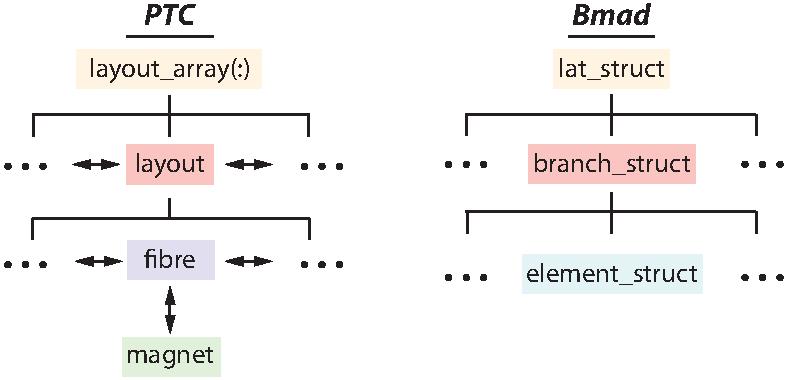
\includegraphics{ptc-structures.pdf}
  \caption[PTC structure relationships] { 
Simplified diagram showing the organization of the major PTC structures involved in
defining a lattice contrasted with \bmad.
  }
\label{f:ptc-struct}
\end{figure}

%--------------------------------------------------------------------------
\section{Variable Initialization and Finalization}
\label{s:ptc.var.init}
\index{PTC/FPP variable!initialization}

PTC variables must be initialized and finalized. This is done with
the\vn{alloc()} and \vn{kill()} routines. In addition, the \vn{real_8_init}
routine can initialize a \vn{real_8} array:
\begin{example}
  type (real_8) y8(6) 
  ...
  call real_8_init (y8)
  call kill (y8)
\end{example}

%--------------------------------------------------------------------------
\section{Correspondence Between Bmad Elements and PTC Fibres}.
\label{s:ele.fib}
\index{fibre}

When a PTC \vn{layout} is created from a \bmad \vn{lat_struct}
instance using the routine
\Hyperref{r:lat.to.ptc.layout}{lat_to_ptc_layout}, the correspondence
between the \bmad elements and the PTC fibres is maintained through
the \vn{ele%ptc_fibre} pointer. The following rules apply:
  \begin{enumerate}
  \item There will be marker \vn{fibre}s at the beginning and end 
of the \vn{layout}. The beginning \vn{fibre} will correspond to
\vn{branch%ele(0)}. The end \vn{fibre} will not have a corresponding
\bmad element.
  \item Generally there will be a one-to-one correspondence between
\vn{fibre}s and \vn{branch%ele} elements. The exception is where a
``hard edge'' model is used for tracking. In this case, there will be
three \vn{fibre}s for the \bmad element: Two drift \vn{fibre}s with a
\vn{fibre} of the appropriate type in between.  In this case,
\vn{ele%ptc_fibre} will point to the last (drift) \vn{fibre}.
  \end{enumerate}

Remember: The attributes like reference energy, etc. for a \bmad
\vn{ele_struct} instance are referenced to the exit end of the
element. For PTC the reference edge for a \vn{fibre} is the entrance
end.

%--------------------------------------------------------------------------
\section{Taylor Maps}
\label{s:ptc.taylor}
\index{PTC/FPP!Taylor Maps}

\index{PTC/FPP!real_8}\index{PTC/FPP!universal_taylor}
FPP stores its \vn{real_8} Taylor maps in such a way that it is not
easy to access them directly to look at the particular terms. To
simplify life, \'Etienne has implemented the
\vn{universal_taylor}structure:
\begin{example}
  type universal_taylor
    integer, pointer  :: n       ! Number of coefficients
    integer, pointer  :: nv      ! Number of variables
    real(dp), pointer :: c(:)    ! Coefficients C(N)
    integer, pointer  :: j(:,:)  ! Exponents of each coefficients J(N,NV)
  end type
\end{example}
\bmad always sets \vn{nv} = 6. \bmad overloads the equal sign to call 
routines to convert between \'Etienne's
\vn{real_8} Taylor maps and \vn{universal_taylor}:
\begin{example}
  type (real_8) tlr(6)           ! Taylor map
  type (universal_taylor) ut(6)  ! Taylor map
  ...
  tlr = ut                       ! Convert universal_taylor -> real_8
  ut = tlr                       ! Convert real_8 -> universal_taylor
\end{example}

%--------------------------------------------------------------------------
\section{Patches}
\label{s:ptc.patch}
\index{PTC/FPP!patch}

There is a significant difference between how patches are treated in
PTC and \bmad.  In PTC, a patch is just though of as a coordinate
transformation for propagating a particle from one \vn{fibre} to the
next. As such, the \vn{patch} is part of a \vn{fibre}. That is, any
\vn{fibre} representing tracking through quadrupoles, bends, etc. will
have patches for the entrance and exit ends of the \vn{fibre}.

With \bmad, on the other hand, a \vn{patch} is a ``first class''
element on par with all other elements be they quadrupoles, bends,
etc. When translating a \vn{patch} from \bmad to PTC, the \vn{patch}
is represented in PTC as a \vn{marker} element with a patch at the
exit end.

%--------------------------------------------------------------------------
\section{Number of Integration Steps \& Integration Order}
\label{s:ptc.step}

``Drift like'' elements in PTC will use, by default, only one
integration step. \bmad uses the default when translating from \bmad
lattice elements to PTC fibres. The \bmad lattice elements that are
drift like are:
\begin{example}
  drift
  ecollimator 
  instrument 
  monitor 
  pipe
  rcollimator 
\end{example}

When tracking, there is a trade-off between step size and integrator order. Higher order
means fewer steps are needed to get the same accuracy. But one higher order step is
computationally more intensive then one lower order step so what is the optimum order and
number of steps is dependent upon various factors like magnet strength and how fast the
field is varying. Generally, when the field is varying, such as in a wiggler, lower order
and more steps are favored. Also spin tracking is always 2nd order in PTC. So going to higher
order for the orbital tracking with less steps will cause the spin tracking to be less
accurate.

The way PTC ``resplitting'' routines work is that, for a given element, they start by
assuming that the tracking will be done using a 2\Nd order integrator, They then compute
the number of steps needed based upon the electric and magnetic field strengths. This
number is compared to a crossover limit point here named $C_1$. If the number of steps is
less than or equal to $C_1$ then the resplitting routine stops and tracking will
thereafter be done with a 2\Nd order integrator with the calculated number of steps. On
the other hand, if the number of steps is greater than $C_1$, the resplitting routine will
redo the calculation assuming 4\Th order integration. With 4\Th order integration, the
number of calculated steps will compared to a different crossover limit point here called
$C_2$. Again, if the number of steps is less than or equal to $C_2$, the routine will
assign 4\Th order tracking to the element. Otherwise, the routine will assign 6\Th order
tracking to the element with an appropriate number of steps.

The default crossover limit points are
\begin{align}
  [C_1, C_2] & = [30, 60] \qquad \text{For wiggler type elements.} \nonumber \\
  [C_1, C_2] & = [4, 18]  \qquad \text{For all other elements.} \nonumber 
\end{align}
The greater number for wigglers is a reflection of the fact that the wiggler field
is not constant.

%--------------------------------------------------------------------------
\section{Creating a PTC layout from a Bmad lattice}
\label{s:ptc.layout}

For a programmer, it is sometimes useful to feed a \bmad lattice into PTC and then use PTC for all
the calculations. As an example of how to do this, the following minimal program creates a PTC
\vn{layout} from a \bmad lattice:
\begin{example}
  use pointer_lattice, dummy => lat
  use ptc_layout_mod, dum1 => dp
  implicit none
  type (lat_struct), target :: lat
  type(layout), pointer:: als
  !
  call bmad_parser ('lat.bmad', lat)
  call lat_to_ptc_layout (lat, .true.)
  als => lat%branch(0)%ptc%m_t_layout
\end{example}

%--------------------------------------------------------------------------
\section{Internal_State}
\label{s:ptc.state}

The \vn{internal_state} structure looks like:
\begin{example}
type internal_state
   integer totalpath      ! total time or path length is used
   logical(lp) time       ! Time is used instead of path length
   logical(lp) radiation  ! Radiation damping (but not excitation) is turned on
   logical(lp) nocavity   ! Cavity is turned into a drift
   logical(lp) fringe     ! fringe fields are turned on (mainly for quadrupoles)
   logical(lp) stochastic ! Random Stochastic kicks to x(5)
   logical(lp) envelope   ! Stochastic envelope terms tracked in probe_8
   logical(lp) para_in    ! If true, parameters in the map are included
   logical(lp) only_4d    ! REAL_8 Taylor in (x,p_x,y,p_y)
   logical(lp) delta      ! REAL_8 Taylor in (x,p_x,y,p_y,delta)
   logical(lp) spin       ! Spin is tracked
   logical(lp) modulation ! One modulated family tracked by probe
   logical(lp) only_2d    ! REAL_8 Taylor in (x,p_x)
   logical(lp) full_way   !
end type internal_state
\end{example}

\endinput

%!!!!!!!!!!!!!!!!!!!!!!!!!!!!!!!!!!!!!!!!!!!!!!!!!!!!!

Placement of magnet in global coordinate system:

TYPE MAGNET_FRAME
   REAL(DP), POINTER,DIMENSION(:)  ::   A   => null()   ! Entrance point
   REAL(DP), POINTER,DIMENSION(:,:)::   ENT => null()   ! Entrance orientation. %ent(1,1:3) => x-axis, etc.
   REAL(DP), POINTER,DIMENSION(:)  ::   O   => null()   ! Mid point. Will be midpoint of chord for a bend.
   REAL(DP), POINTER,DIMENSION(:,:)::   MID => null()
   REAL(DP), POINTER,DIMENSION(:)  ::   B   => null()   ! Exit point
   REAL(DP), POINTER,DIMENSION(:,:)::   EXI => null()
END TYPE MAGNET_FRAME

%% \include{fpp}
\chapter{OPAL}
\label{c:opal}
\index{OPAL}
%----------------------------------------------------------------------------

OPAL (Object Oriented Parallel Accelerator Library) is a tool for charged-particle optic
calculations in large accelerator structures and beam lines including 3D space charge. OPAL is built
from first principles as a parallel application, OPAL admits simulations of any scale: on the laptop
and up to the largest High Performance Computing (HPC) clusters available today. Simulations, in
particular HPC simulations, form the third pillar of science, complementing theory and experiment.

OPAL includes various beam line element descriptions and methods for single particle optics, namely
maps up to arbitrary order, symplectic integration schemes and lastly time integration. OPAL is
based on IPPL (Independent Parallel Particle Layer) which adds parallel capabilities. Main functions
inherited from IPPL are: structured rectangular grids, fields and parallel FFT and particles with
the respective interpolation operators. Other features are, expression templates and massive
parallelism (up to 8000 processors) which makes is possible to tackle the largest problems in the
field.

The  manual can be obtained at
\begin{example} 
  amas.web.psi.ch/docs/opal/   
\end{example}

%--------------------------------------------------------------------------
\section{Phase Space}
\label{s:opal.space}
\index{OPAL!phase space}

OPAL uses different longitudinal phase space coordinates compared to \bmad.  \bmad's phase space
coordinates are
\begin{equation}
  (x, p_x/p_0, y, p_y/p0, -\beta c (t - t_0), (p-p_0)/p_0)
\end{equation}
OPAL uses
\begin{equation}
  (x, \gamma \beta_x,  y, \gamma \beta_y, z, \gamma \beta_z)
\end{equation}
\vn{convert_particle_coordinates_s_to_t} and \vn{convert_particle_coordinates_s_to_t} are conversion routines \ldots

%%--------------------------------------------------------------------------
%\section{Initialization}
%\label{s:etienne.init}
%\index{PTC/FPP!initialization}
%
%One important parameter in PTC is the order of the Taylor maps.
%By default \bmad will set this to 3. The order can be set within
%a lattice file using the \vn{parameter[taylor_order]} attribute.
%In a program the order can be set using \vn{set_ptc}. In fact
%\vn{set_ptc} must be called by a program before PTC can be used.
%\vn{bmad_parser} will do this when reading in a lattice file.
%That is, if a program does not use \vn{bmad_parser} then to use PTC it
%must call \vn{set_ptc}. Note that resetting PTC to a different order
%reinitializes PTC's internal memory so one must be careful if one wants
%to change the order in mid program.
%
%%--------------------------------------------------------------------------
%\section{Taylor Maps}
%\label{s:etienne.taylor}
%\index{PTC/FPP!Taylor Maps}
%
%\index{PTC/FPP!real_8}\index{PTC/FPP!universal_taylor}
%FPP stores its \vn{real_8} Taylor maps in such a way that it is not
%easy to access them directly to look at the particular terms. To
%simplify life, \'Etienne has implemented the
%\vn{universal_taylor}structure:
%\begin{example}
%  type universal_taylor
%    integer, pointer  :: n       ! Number of coefficients
%    integer, pointer  :: nv      ! Number of variables
%    real(dp), pointer :: c(:)    ! Coefficients C(N)
%    integer, pointer  :: j(:,:)  ! Exponents of each coefficients J(N,NV)
%  end type
%\end{example}
%\bmad always sets \vn{nv} = 6. \bmad overloads the equal sign to call 
%routines to convert between \'Etienne's
%\vn{real_8} Taylor maps and \vn{universal_taylor}:
%\begin{example}
%  type (real_8) tlr(6)           ! Taylor map
%  type (universal_taylor) ut(6)  ! Taylor map
%  ...
%  tlr = ut                       ! Convert universal_taylor -> real_8
%  ut = tlr                       ! Convert real_8 -> universal_taylor
%\end{example}

\chapter{C++ Interface}
\label{c:cpp.interface}
\index{C++ interface}

To ease the task of using \cpp routines with \bmad, there is a
library called \vn{cpp_bmad_interface} which implements a set of \cpp
classes in one--to--one correspondence with the major \bmad
structures. In addition to the \cpp classes, the \bmad library
defines a set of conversion routines to transfer data values between
the \bmad Fortran structures and the corresponding \cpp classes.

The list of all classes is given in the file
\begin{example}
  cpp_bmad_interface/include/cpp_bmad_classes.h
\end{example}
The general rule is that the equivalent class to a \bmad structure
named \vn{xxx_struct} will be named \vn{CPP_xxx}. Additionally, for
each \bmad structure, there is a opaque class named \vn{Bmad_xxx_class}
for use in the translation code discussed below. The names of these
opaque classes have the form \vn{Bmad_xxx_class} and are used to define
pointer instances in routine argument lists.

%----------------------------------------------------------------------------
\section{C++ Classes and Enums}
\index{C++ interface!classes}

Generally, The \cpp classes have been set up to simply mirror the
corresponding \bmad structures. For example, the \vn{CPP_lat} class
has a string component named \vn{.version} that mirrors the
\vn{%version} component of the \vn{lat_struct} structure. There are
some exceptions. For example, structure components that are part of
\vn{PTC} (\sref{s:ptc.intro}) are not present in the classes.

While generally the same component name is used for both the \bmad
structures and the \cpp classes, in the case where there is a \cpp
reserved word conflict, the \cpp component name will be different.

A header file \vn{bmad_enums.h} defines corresponding \bmad
parameters for all \cpp routine. The \bmad parameters are in a
namespace called \vn{Bmad}. The convention is that the name of a
corresponding \cpp parameter is obtained by dropping the ending
\vn{\$} (if there is one) and converting to uppercase. For example,
\vn{electron\$} on the Fortran side converts to \vn{Bmad::ELECTRON} in
\cpp. 

All of the \cpp class components that are arrays or matrices are zero
based so that, for example, the index of the \vn{.vec[i]} array in a
\vn{CPP_coord} runs from 0 through 5 and not 1 through 6 as on the
Fortran side. Notice that for a \vn{lat_struct} the \vn{%ele(0:)}
component has a starting index of zero so there is no off--by--one
problem here.  The exception to this rule is the \vn{%value(:)} array
of the \vn{ele_struct} which has a span from 1 to
\vn{num_ele_attrib\$}. In this case, To keep the conversion of the of
constructs like \vn{ele%value(k1\$)} consistant, the corresponding
\vn{ele.value[]} array has goes from 0 to \vn{Bmad::NUM_ELE_ATTRIB}
with the 0th element being unused.

%----------------------------------------------------------------------------
\section{Conversion Between Fortran and C++}
\index{C++ interface!Fortran calling C++}

\begin{figure}[tb]
\begin{listing}{1}
  subroutine f_test
    use bmad_cpp_convert_mod
    implicit none

    interface
      subroutine cpp_routine (f_lat, c_coord) bind(c)
        import f_lat, c_ptr
        type (lat_struct) :: f_lat
        type (c_ptr), value :: c_coord
      end subroutine
    end interface

    type (lat_struct), target :: lattice   // lattice on Fortran side 
    type (coord_struct), target :: orbit
    type (c_ptr), value :: c_lat
    ! ... 
    call lat_to_c (c_loc(lattice), c_lat)    ! Fortran side convert
    call cpp_routine (c_lat, c_loc(orbit))   ! Call C++ routine
    call lat_to_f (c_lat, c_loc(lattice))    ! And convert back
  end subroutine
\end{listing}
\caption{Example Fortran routine calling a \cpp routine.}
\label{f:fortran}
\end{figure}


\begin{figure}
\begin{listing}{1}
  #include "cpp_bmad_classes.h"

  using namespace Bmad;

  extern "C" cpp_routine (CPP_lat& c_lat, Bmad_coord_class* f_coord,  f_lat) {
    CPP_coord c_coord;
    coord_to_c (f_coord, c_coord);        // C++ side convert
    // ... do calculations ...
    cout << c_lat.name << "  " << c_lat.ele[1].value[K1] << endl;
    coord_to_f (c_coord, f_coord);        // And convert back
  }
\end{listing}
\caption{Example \cpp routine callable from a Fortran routine.}
\label{f:cpp}
\end{figure}

A simple example of a Fortran routine calling a \cpp routine is shown
in \figs{f:fortran} and \ref{f:cpp}. Conversion between structure and
classes can happen on either the Fortran side or the \cpp side. In
this example, the \vn{lat_struct} / \vn{CPP_lat} conversion is on the
Fortran side and the \vn{coord_struct} / \vn{CPP_coord} is on the \cpp
side. 

On the Fortran side, the interface block defines the argument list of
the \cpp routine being called.

On the \cpp side, \vn{f_coord} is an instance of the
\vn{Bmad_coord_class} opaque class.

A \cpp routine calling a Fortran routine has a similar structure to
the above example. The interface block in \fig{f:fortran} can be used
as a prototype. For additional examples of conversion between Fortran
and \cpp, look at the test code in the directory
\begin{example}
  cpp_bmad_interface/interface_test
\end{example}

\chapter{Quick_Plot Plotting}
\label{c:quick.plot}
\index{quick_plot|hyperbf}
\index{pgplot!and Quick_Plot}

\quickplot is an interface layer to either the \vn{PGPLOT}\cite{b:pgplot} or
\vn{PLPLOT}\cite{b:plplot} plotting libraries. Whether \vn{PGPLOT} or \vn{PLPLOT} is used depends upon
an environmental switch set when the \bmad library and other associated libraries are compiled
(\sref{s:libs}). [Note: \quickplot lives in the \vn{sim_utils} library which comes with the Bmad
distribution.] A quick reference guide can be seen online by using the command \vn{getf
quick_plot}. For identification in a program, all \quickplot subroutines start with a \vn{qp_}
prefix. Also, by convention, all PGPLOT subroutines start with a \vn{pg} prefix.

%----------------------------------------------------------------------------

\begin{figure}
\index[routine]{qp_open_page}
\index[routine]{qp_close_page}
\index[routine]{qp_read_data}
\index[routine]{qp_calc_and_set_axis}
\index[routine]{qp_draw_text}
\index[routine]{qp_draw_axes}
\index[routine]{qp_draw_data}
\index[routine]{qp_save_state}
\index[routine]{qp_restore_state}
\index[routine]{qp_set_page_border}
\index[routine]{qp_set_margin}
\index[routine]{qp_set_line_attrib}
\index[routine]{qp_set_box}
\index[routine]{qp_set_graph_attrib}
\index[routine]{qp_set_symbol_attrib}
\index[routine]{qp_set_axis}
\footnotesize
\begin{listing}{1}
  program example_plot
    use quick_plot
    integer id
    character(1) ans
  
    ! Generate PS and X-windows plots.
    call qp_open_page ("PS-L")  ! Tell \quickplot to generate a PS file.
    call plot_it              ! Generate the plot
    call qp_close_page        ! quick_plot.ps is the file name
    call qp_open_page ("X", id, 600.0_rp, 470.0_rp, "POINTS")
    call plot_it
    write (*, "(a)", advance = "NO") " Hit any class to end program: "
    accept "(a)", ans

  !----------------------------------------------------------------------
  contains
  subroutine plot_it                             ! This generates the plot
    real(rp), allocatable :: x(:), y(:), z(:), t(:)
    real(rp) x_axis_min, x_axis_max, y_axis_min, y_axis_max
    integer x_places, x_divisions, y_places, y_divisions
    character(80) title
    logical err_flag
    namelist / parameters / title

    ! Read in the data
    open (1, file = "plot.dat", status = "old")
    read (1, nml = parameters)                  ! read in the parameters.
    call qp_read_data (1, err_flag, x, 1, y, 3, z, 4, t, 5) ! read in the data.
    close (1)

    ! Setup the margins and page border and draw the title
    call qp_set_page_border (0.01_rp, 0.02_rp, 0.2_rp, 0.2_rp, "%PAGE")
    call qp_set_margin (0.07_rp, 0.05_rp, 0.05_rp, 0.05_rp, "%PAGE")
    call qp_draw_text (title, 0.5_rp, 0.85_rp, "%PAGE", "CT") 

    ! draw the left graph
    call qp_set_box (1, 1, 2, 1)
    call qp_calc_and_set_axis ("X", minval(x), maxval(x), 4, 8, "ZERO_AT_END")
    call qp_calc_and_set_axis ("Y", minval(z), maxval(z), 4, 8, "GENERAL")
    call qp_draw_axes ("X\dlab\u", "\gb(\A)")
    call qp_draw_data (x, y, symbol_every = 0)

    call qp_save_state (.true.)
    call qp_set_symbol_attrib ('times', color = "blue", height = 20.0_rp)
    call qp_set_line_attrib ("PLOT", color = "blue", style = "dashed")
    call qp_draw_data (x, z, symbol_every = 5)
    call qp_restore_state

    ! draw the right graph. "star5_filled" is a five pointed star.
    call qp_save_state (.true.)
    call qp_set_box (2, 1, 2, 1)
    call qp_set_graph_attrib (draw_grid = .false.)
    call qp_set_symbol_attrib ('star5_filled', height = 10.0_rp)
    call qp_set_axis ("Y", -0.1_rp, 0.1_rp, 4, 2)
    call qp_set_axis ('Y2', 1.0_rp, 100.0_rp, label = "Y2 axis", &
                                draw_numbers = .true., ax_type = "LOG")
    call qp_draw_axes ("\m1 \m2 \m3 \m4 \m5 \m6 \m7", "\fsLY\fn", title = "That Darn Graph")
    call qp_draw_data (x, t, draw_line = .false., symbol_every = 4)
    call qp_restore_state
  end subroutine
  end program
\end{listing}
\caption{\quickplot example program.}
\label{f:plot.example}
\end{figure}


\begin{figure}
\centering
\includegraphics[width=5.5in]{plot-example.pdf}
\caption{Output of plot_example.f90.}
\label{f:plot.out}
\end{figure}

%----------------------------------------------------------------------------
\section{An Example}
\label{s:plot.example}

An example of how \quickplot can be used in a program is shown in
\fig{f:plot.example}. In the \bmad distribution a copy of this
program is in the file
\begin{example}
  sim_utils/plot_example/plot_example.f90
\end{example}
The \vn{plot_example.f90} program generates the figure shown in
\fig{f:plot.out} from the input file named \vn{plot.dat}. The
first few lines of the data file are
\begin{example}
  \&parameters
    title = "A Tale of Two Graphs"
  /
 
  Any junk here...
 
  Col1      Col2      Col3      Col4      Col5
     0    0.0000    0.1000    0.0000   -0.0125
     1    0.0001    0.0995    0.0101   -0.0127
     2    0.0004    0.0980    0.0203   -0.0130
     3    0.0009    0.0955    0.0304   -0.0132
     ...
\end{example}

The program first creates a PostScript file for printing on lines 7
through 9 and then makes an X--windows plot on lines 10 and 11. The
write/accept lines 12 and 13 are to pause the program to prevent the
X-window from immediately closing upon termination of the program.

The heart of the plotting is in the subroutine \vn{plot_it} beginning
on line 17. The namelist read on line 27 shows how both parameters and
data can be stored in the same file so that a plotting program can be
automatically told what the appropriate plot labels are. The
\Hyperref{r:qp.draw.text}{qp_draw_text} call on line 34 draws the 
title above the two graphs.

The \Hyperref{r:qp.read.data}{qp_read_data} call on line 28 will skip
any ``header'' lines (lines that do not begin with something that looks
like a number) in the data file. In this instance
\Hyperref{r:qp.read.data}{qp_read_data} will read the first, third forth
and fifth data columns and put them into the \vn{x}, \vn{y}, \vn{z}, and
\vn{t} arrays.

\Hyperref{r:qp.set.page.border}{qp_set_page_border},
\Hyperref{r:qp.set.box}{qp_set_box}, and
\Hyperref{r:qp.set.margin}{qp_set_margin} sets where the graph is
going to be placed.  \Hyperref{r:qp.set.box}{qp_set_box}\vn{(1, 1, 2,
1)} on line 37 tells \quickplot to put the first graph in the left box
of a 2 box grid. The \Hyperref{r:qp.set.margin}{qp_set_margin} on line
33 sets the margins between the box and the graph axes.

\Hyperref{r:qp.calc.and.set.axis}{qp_calc_and_set_axis} on lines 38
and 39 are used to scale the axes. \vn{"ZERO_AT_END"} ensures that the
$x$--axis starts (or stops) at zero.
\Hyperref{r:qp.calc.and.set.axis}{qp_calc_and_set_axis} is told to
restrict the number of major divisions to be between 4 and 8. For the
horizontal axis, as can be seen in \fig{f:plot.out}, it chooses
5 divisions.

After drawing the first data curve (the solid curve) in the left
graph, the routines
\Hyperref{r:qp.set.symbol.attrib}{qp_set_symbol_attrib} and
\Hyperref{r:qp.set.line.attrib}{qp_set_line_attrib} are called on
lines 44 and 45 to plot the next data curve in blue with a dashed line
style. By default, this curve goes where the last one did: in the left
graph. To keep the setting of the line and symbol attributes from
affecting other plots the routines
\Hyperref{r:qp.save.state}{qp_save_state} and
\Hyperref{r:qp.restore.state}{qp_restore_state} on lines 43 and 47 are
used. \Hyperref{r:qp.save.state}{qp_save_state} saves the current
attributes in an attribute
stack. \Hyperref{r:qp.restore.state}{qp_restore_state} restores the
saved attributes from the attribute
stack. \Hyperref{r:qp.draw.axes}{qp_draw_axes} is called on line 40 to
draw the $x$ and $y$-axes along, and \vn{qp_draw_data} is called on
lines 41 and 46 to draw the two data curves.

Lines 50 through 60 draw the third curve in the right hand graph.  The
\vn{qp_set_axis} call on lines 55/56 sets a log scale for the \vn{y2}
(right hand) axis. The syntax of the string arguments of
\Hyperref{r:qp.draw.axes}{qp_draw_axes} in lines 40 and 57/58 comes from PGPLOT and allows
special symbols along with subscripts and superscripts.

%----------------------------------------------------------------------------
\section{Plotting Coordinates}
\label{s:plot.coords}

\begin{figure}
  \centering
  \includegraphics{plot-coords.pdf}
  \caption{A Graph within a Box within a Page.}
  \label{f:plot.coords}
\end{figure}

\quickplot uses the following concepts as shown in \fig{f:plot.coords}
\begin{example}
  PAGE  -- The entire drawing surface.
  BOX   -- The area of the page that a graph is placed into.
  GRAPH -- The actual plotting area within the bounds of the axes.
\end{example}
In case you need to refer to the PGPLOT routines the correspondence
between this and PGPLOT is:
\begin{example}
  QUICK_PLOT    PGPLOT
  ----------    ------
  PAGE          VIEW SURFACE
  BOX           No corresponding entity.
  GRAPH         VIEWPORT and WINDOW
\end{example}
Essentially the VIEWPORT is the region outside of which lines and symbols
will be clipped (if clipping is turned on) and the WINDOW defines the
plot area. I'm not sure why PGPLOT makes a distinction, but VIEWPORT and
WINDOW are always the same region.

\Hyperref{r:qp.open.page}{qp_open_page} determines the size of the \vn{page} if it is
settable (like for X--windows). The page is divided up into a grid of
boxes. For example, in \fig{f:plot.coords}, the grid is 1 box
wide by 3 boxes tall. The border between the grid of boxes and the
edges of the page are set by \Hyperref{r:qp.set.page.border}{qp_set_page_border}.  The box that
the graph falls into is set by \Hyperref{r:qp.set.box}{qp_set_box}. The default is to
have no margins with 1 box covering the entire page. The
\Hyperref{r:qp.set.margin}{qp_set_margin} routine sets the distance between the box edges
and the axes (See the PGPLOT manual for more details).


%----------------------------------------------------------------------------
\section{Length and Position Units}
\label{s:plot.units}
\index{quick_plot!position units}

Typically there is an optional \vn{units} argument for \quickplot routines that
have length and/or position arguments. For example, using \vn{getf} one can
see that the arguments for \Hyperref{r:qp.draw.rectangle}{qp_draw_rectangle} are
\begin{example}
  Subroutine qp_draw_rectangle (x1, x2, y1, y2, units, color, width, style, clip)
\end{example}
The \vn{units} argument is a character string which is divided into three
parts. The syntax of the \vn{units} argument is
\begin{example}
  unit_type/ref_object/corner
\end{example}
The first part \vn{unit_type} gives the type of units
\begin{example}
  "%"       -- Percent.
  "DATA"    -- Data units. (Draw default)
  "MM"      -- millimeters.
  "INCH"    -- Inches. (Set default)
  "POINTS"  -- Printers points. NOT PIXELS. (72 points = 1 inch).
\end{example}
Note: For displays with a resolution of 72 pixels / inch, \vn{POINTS} corresponds to pixels but
many displays have a higher resolution.
The second and third parts give the reference point for a position.
The second part specifies the reference object
\begin{example}
    "PAGE"  -- Relative to the page (Set default).
    "BOX"   -- Relative to the box.
    "GRAPH" -- Relative to the graph (Draw default).
\end{example}
The third part gives corner of the reference object that is the reference point
\begin{example}
    "LB"    -- Left Bottom (Set and Draw default).
    "LT"    -- Left Top.
    "RB"    -- Right Bottom.
    "RT"    -- Right Top.
\end{example}

Notes:
\begin{itemize}
 \item 
The \vn{DATA} unit type, by definition, always uses the lower left
corner of the \vn{GRAPH} as a reference point.
 \item 
For the \vn{%} \vn{unit_type} the \vn{/} between \vn{unit_type} 
and \vn{ref_object} can be omitted.
 \item 
If the \vn{corner} is specified then the \vn{ref_object} must appear also.
 \item 
Everything must be in upper case.
 \item 
For some routines (\Hyperref{r:qp.set.margin}{qp_set_margin}, etc.) only a relative distance
is needed. In this case the \vn{ref_object/corner} part, if present,
is ignored.
 \item 
The \vn{units} argument is typically an optional argument. If not
present the default units will be used. There are actually two
defaults: The draw default is used for drawing text, symbols, or whatever.
The set default is used for setting margins, and other lengths.
Initially the draw default is \vn{DATA/GRAPH/LB} and the set
default is \vn{INCH/PAGE/LB}. 
Use \Hyperref{r:qp.set.parameters}{qp_set_parameters} to change this.
\end{itemize}
Examples:
\begin{example}
  "DATA"          -- This is the draw default. 
  "DATA/GRAPH/LB" -- Same as above.
  "DATA/BOX/RT"   -- ILLEGAL: DATA must always go with GRAPH/LB.
  "%PAGE/LT"      -- Percentage of page so (0.0, 1.0) = RT of page.
  "%BOX"          -- Percentage of box so (1.0, 1.0) = RT of box.
  "INCH/PAGE"     -- Inches from LB of page.
\end{example}

%----------------------------------------------------------------------------
\section{Y2 and X2 axes}
\label{s:axes2}
\index{quick_plot!axes}

The top and right axes of a graph are known as \vn{X2} and \vn{Y2}
respectively as shown in \fig{f:plot.coords}. Normally the
\vn{X2} axis mirrors the \vn{X} axis and the \vn{Y2} axis mirrors the
\vn{Y} axis in that the tick marks and axis numbering for the \vn{X2}
and \vn{Y2} axes are the same as the \vn{X} and \vn{Y} axes
respectively. \Hyperref{r:qp.set.axis}{qp_set_axis} can be used to disable mirroring. For
example:
\begin{example}
  call qp_set_axis ("Y2", mirror = .false.)  ! y2-axis now independent of y.
\end{example}
\Hyperref{r:qp.set.axis}{qp_set_axis} can also be used to set \vn{Y2} axis parameters
(axis minimum, maximum, etc.) and setting the \vn{Y2} or \vn{X2} axis
minimum or maximum will, by default, turn off mirroring.

Note that the default is for the \vn{X2} and \vn{Y2} axis numbering
not to be shown. To enable or disable axis numbering again use
\Hyperref{r:qp.set.axis}{qp_set_axis}. For example:
\begin{example}
  call qp_set_axis ("Y2", draw_numbers = .true.)  ! draw y2 axis numbers
\end{example}

To plot data using the \vn{X2} or \vn{Y2} scale use the
\Hyperref{r:qp.use.axis}{qp_use_axis} routine. For example:
\begin{example}
  call qp_save_state (.true.)
  call qp_use_axis (y = "Y2")
  ! ... Do some data plotting here ...
  call qp_restore_state
\end{example}

%----------------------------------------------------------------------------
\section{Text}
\label{s:text}

PGPLOT defines certain escape sequences that can be used in text strings to draw Greek letters,
etc. These escape sequences are given in Table~\ref{t:pgplot.escape}.

PGPLOT defines a text background index:
\begin{example}
         -1 - Transparent background.
          0 - Erase underlying graphics before drawing text.
   1 to 255 - Opaque with the number specifying the color index.
\end{example}

%----------------------------------------------------------------------------
\section{Styles}
\label{s:styles}

Symbolic constants have been defined for \quickplot subroutine arguments that are used to choose
various styles. As an example of this is in lines 44 and 45 of \fig{f:plot.example}. The numbers in
the following are the PGPLOT equivalents.

\index{quick_plot!line styles}
The \quickplot line styles are:
\begin{example}
    1 -- solid\$                  Solid
    2 -- dashed\$                 Dashed
    3 -- dash_dot\$               Dash--dot 
    4 -- dotted\$                 Dotted
    5 -- dash_dot3\$              Dash--dot--dot--dot        
\end{example}

\index{quick_plot!color styles}
The color styles in \quickplot are:
\begin{example}
    0 -- White\$   (actually the background color)
    1 -- Black\$   (actually the foreground color)
    2 -- Red\$
    3 -- Green\$
    4 -- Blue\$
    5 -- Cyan\$
    6 -- Magenta\$
    7 -- Yellow\$ 
    8 -- Orange\$
    9 -- Yellow_Green\$
   10 -- Light_Green\$
   11 -- Navy_Blue\$
   12 -- Purple\$
   13 -- Reddish_Purple\$
   14 -- Dark_Grey\$
   15 -- Light_Grey\$
\end{example}
   
Integers from [17, (largest integer)] represent continuous colors. The function \vn{pq_continuous_color} maps [0.0, 1.0] to these integers. See Fig.~\ref{f:plot-continuous-color}.

\begin{figure}
\centering
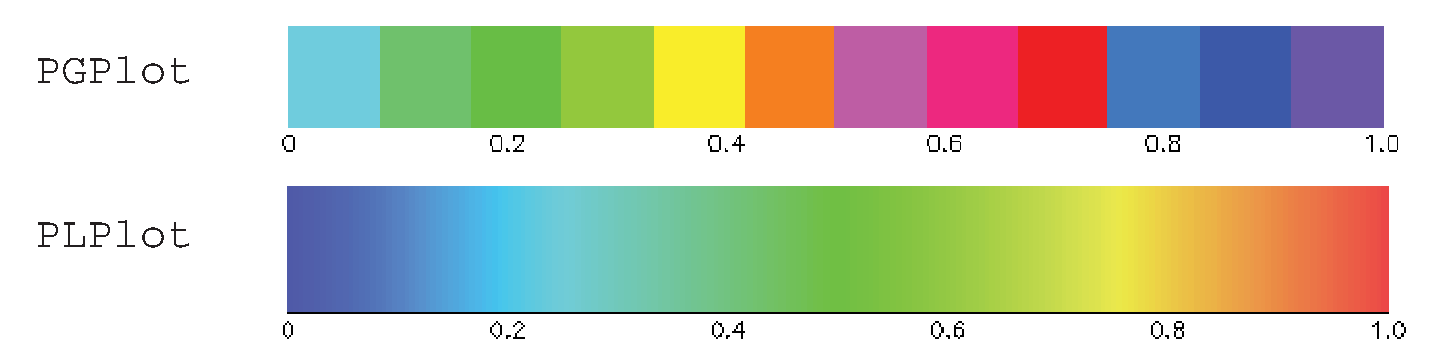
\includegraphics[width=0.8\textwidth]{plot-continuous-color.pdf}
\caption{Continuous colors using the function \vn{pg_continuous_color} in PGPlot and PLPlot. Typical usage: \vn{call qp_routine(..., color = pg_continuous_color(0.25_rp), ...)}}
\label{f:plot-continuous-color}
\end{figure}

\index{quick_plot!fill styles}
The fill styles are:
\begin{example}
    1 -- solid_fill\$        
    2 -- no_fill\$           
    3 -- hatched\$           
    4 -- cross_hatched\$     
\end{example}

\index{quick_plot!symbol styles}
The symbol types are:
\begin{example}
    0 -- square_sym\$
    1 -- dot_sym\$
    2 -- plus_sym\$
    3 -- times_sym\$
    4 -- circle_sym\$
    5 -- x_sym\$
    7 -- triangle_sym\$
    8 -- circle_plus_sym\$
    9 -- circle_dot_sym\$
   10 -- square_concave_sym\$
   11 -- diamond_sym\$
   12 -- star5_sym\$
   13 -- triangle_filled_sym\$
   14 -- red_cross_sym\$
   15 -- star_of_david_sym\$
   16 -- square_filled_sym\$
   17 -- circle_filled_sym\$
   18 -- star5_filled_sym\$
\end{example}
Beside this list, PGPLOT maps other numbers onto symbol types. 
The PGPLOT list of symbols is:
\begin{example}
  -3 ... -31 - a regular polygon with abs(type) edges.
          -2 - Same as -1.
          -1 - Dot with diameter = current line width.
   0 ...  31 - Standard marker symbols.
  32 ... 127 - ASCII characters (in the current font).
                  E.G. to use letter F as a marker, set type = ICHAR("F"). 
       > 127 - A Hershey symbol number.
\end{example}
Table~\ref{t:plot.syms} shows some of the symbols and there associated 
numbers. Note: At constant height PGPLOT gives symbols of different size.
To partially overcome this, \quickplot scales some of the symbols to
give a more uniform appearance. Table~\ref{t:plot.syms} was generated
using a height of 40 via the call
\begin{example}
  call qp_draw_symbol (0.5_rp, 0.5_rp, "%BOX", k, height = 40.0_rp)
\end{example}

\index{quick_plot!symbol table}
\begin{table}
  \centering
  \includegraphics{plot-syms.pdf}
  \caption{Plotting Symbols at Height = 40.0}
  \label{t:plot.syms}
\end{table}

\begin{table}
\begin{tabular}{ll} \toprule
{\B}u       & Start a superscript or end a subscript \\[0.5ex]
{\B}d       & Start a subscript or end a superscript.
              {\B}u and {\B}d must always be used in pairs \\[0.5ex]
{\B}b       & Backspace (i.e., do not advance text pointer  
               after plotting the previous character) \\[0.5ex]
{\B}fn      & Switch to Normal font (1)       \\[0.5ex]
{\B}fr      & Switch to Roman font (2)        \\[0.5ex]
{\B}fi      & Switch to Italic font (3)       \\[0.5ex]
{\B}fs      & Switch to Script font (4)       \\[0.5ex]
{\B}{\B}    & Backslash character (\B)        \\[0.5ex]
{\B}x       & Multiplication sign ($\times$)  \\[0.5ex]
{\B}.       & Centered dot ($\cdot$)          \\[0.5ex]
{\B}A       & Angstrom symbol (\AA)         \\[0.5ex]
{\B}gx      & Greek letter corresponding to roman letter x \\[0.5ex]
{\B}mn {\B}mnn & Graph marker number $n$ or $nn$ (1-31) \\[1ex]
{\B}(nnnn)  & 
\parbox{4.8in}{\setstretch{0.5} Character number nnnn (1 to 4 decimal digits) from the
Hershey character set; the closing parenthesis may be omitted if the
next character is neither a digit nor ``)''. This makes a number of
special characters (e.g., mathematical, musical, astronomical, and
cartographical symbols) available.} \\ \bottomrule
\end{tabular}
\caption{PGPLOT Escape Sequences.}
\label{t:pgplot.escape}
\end{table}

Table~\ref{t:greek} shows how the character string \vn{"{\B}g<r>"}, where \vn{"<r>"} 
is a Roman letter, map onto the Greek character set.
\begin{table}
  \centering
  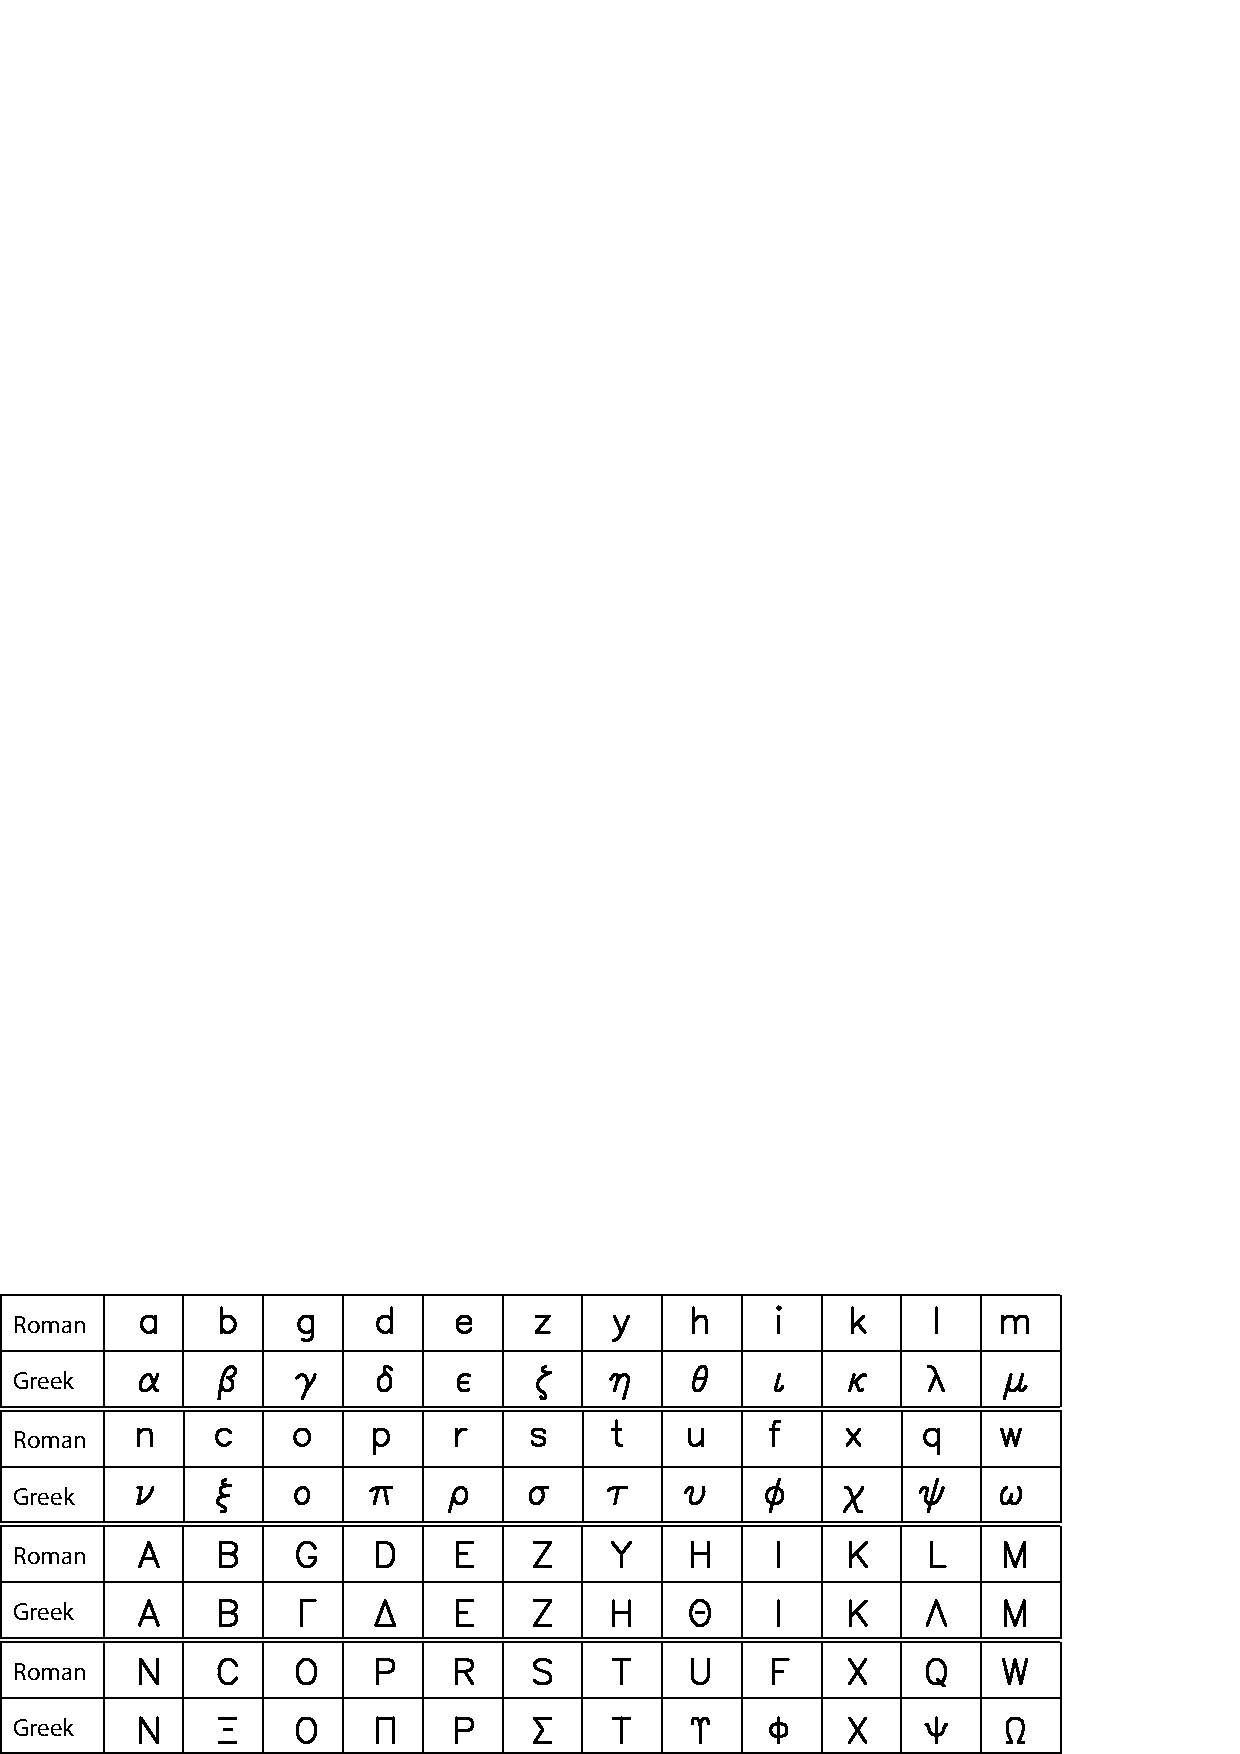
\includegraphics[width=5.5in]{greek.pdf}
  \caption[Roman to Greek Character Conversion]{Conversion for the string 
\vn{"{\B}g<r>"} where \vn{"<r>"} is a Roman character to the corresponding 
Greek character.}
\label{t:greek}
\end{table}


%----------------------------------------------------------------------------
\section{Structures}
\label{s:qp.structs}
\index{quick_plot!structures}

\index{qp_line_struct}
\quickplot uses several structures to hold data. The structure that
defines a line is a \vn{qp_line_struct}
\begin{example}
  type qp_line_struct
    integer width         ! Line width.   Default = 1
    character(16) color   ! Line color.   Default = "black"
    character(16) pattern ! line pattern. Default = "solid"
  end type
\end{example}

\index{qp_symbol_struct}
The \vn{qp_symbol_struct} defines how symbols are drawn 
\begin{example}
  type qp_symbol_struct
    character(16)  type        ! Default = "circle_dot"
    real(rp) height            ! Default = 6.0 (points)
    character(16)  color       ! Default = "black"
    character(16)  fill        ! Default = "solid_fill"
    integer  line_width        ! Default = 1
  end type
\end{example}

\index{qp_axis_struct}
The \vn{qp_axis_struct} defines how axes are drawn 
\begin{example}
  type qp_axis_struct
    character(80) label       ! Axis label.
    real(rp) min              ! Axis range left/bottom number.
    real(rp) max              ! Axis range right/top number.
    real(rp) number_offset    ! Offset in inches of numbering from the axis line. 
                              !  Default = 0.05
    real(rp) label_offset     ! Offset in inches of the label from the numbering.
                              !  Default = 0.05
    character(16) label_color ! Default = "black"
    real(rp) major_tick_len   ! Length of the major ticks in inches. Def = 0.10
    real(rp) minor_tick_len   ! Length of the minor ticks in inches. Def = 0.06
    integer major_div         ! Number of major divisions. Default = 5
    integer major_div_nominal ! Nominal value. Def = 5.
    integer minor_div         ! Number of minor divisions. 0 = auto-choose. Default = 0
    integer minor_div_max     ! Maximum number for auto choose. Default = 5
    integer places            ! Places after the decimal point. Default = 0
    character(16) type        ! "LINEAR" (default), "LOG", or "CUSTOM".
    character(16) bounds      ! "GENERAL" (default), "ZERO_AT_END", etc.
    integer tick_side         ! +1 = draw to the inside (def), 0 = both, -1 = outside.
    integer number_side       ! +1 = draw to the inside, -1 = outside (default).
    logical draw_label        ! Draw the label? Default = True.
    logical draw_numbers      ! Draw the numbering? Default = True.
  end type
\end{example}

The \vn{%bounds} parameter sets how axis min and max values are calculated. Possible settings are:
\begin{example}
  "ZERO_AT_END"      ! Min or max value is set to zero.
  "ZERO_SYMMETRIC"   ! Min and max chosen so that max = -min.
  "GENERAL"          ! No restrictions.
  "EXACT"            ! The inputted data min/max is used.
\end{example}

Finally, the \vn{qp_plot_struct} is a container for the axis that make up a plot
\begin{example}
  type qp_plot_struct
    character(80) :: title = " "
    type (qp_axis_struct) x, y, x2, y2
    type (qp_axis_struct), pointer :: xx, yy  ! Pointer to axes used for plotting.
    logical :: draw_box    = .true.
    logical :: draw_title  = .true.
    logical :: draw_grid   = .true.
    logical :: x2_mirrors_x = .true.
    logical :: y2_mirrors_y = .true.
    logical :: xx_points_to_x
    logical :: yy_points_to_y
  end type
\end{example}

%\end{document}

\chapter{HDF5}
\label{c:hdf5}
\index{hdf5}

\vn{HDF5}, which stands for ``Hierarchical Data Format'' version 5\cite{b:hdf5}, is a set of file
formats designed to store and organize large amounts of data. HDF5 has been developed by scientists
from a number of institutions including the National Center for Supercomputing Applications, the
University of Illinois at Urbana-Champaign, and Sandia National Laboratories. Tools for viewing and
editing HDF5 files are available from the HDF Group\cite{b:hdf5}. Programs include \vn{h5dump} and
\vn{HDFView} which can be used to directly view files. Interfaces so that HDF5 files can accessed
via Java or Python also exist.

\bmad uses HDF5 for storing beam particle (positions, spin, etc.) and \vn{grid_field}
(\sref{s:grid.field}) data. Storage details are given in sections \sref{s:hdf5.beam} and
\sref{s:hdf5.grid} respectively. While \vn{HDF5} defines how data is formatted, \vn{HDF5} does not
define the syntax for how data is to be stored. For that, \bmad uses the syntax defined by the
\vn{Beam Physics} extension to the \vn{openPMD} standard\cite{b:openpmd}. To understand the rest of
this chapter, the reader should familiarize themselves with the \vn{openPMD} and \vn{Beam Physics}
standards.

%-----------------------------------------------------------------
\section{HDF5 Particle Beam Data Storage}
\label{s:hdf5.beam}
\index{hdf5 and particle beam data}

The code for reading and writing beam data to/from HDF5 files is contained in the routines
\Hyperref{r:hdf5.read.beam}{hdf5_read_beam} and \Hyperref{r:hdf5.write.beam}{hdf5_write_beam}.

As per the \vn{openPMD}/\vn{Beam Physics} standard, particle beam data is stored in a tree structure
within a data file. The root ``\vn{group}'' (tree node) for each bunch of the beam has the path
within the file:
\begin{example}
  /data/%T/particles/
\end{example}
where \vn{%T} is an integer.

For any bunch, parameters (``attributes'') stored in the bunch root group are:
\begin{example}
  speciesType     ! The name of the particle species using the \vn{SpeciesType} syntax.
  totalCharge     ! Total bunch charge.
  chargeLive      ! Charge of live particles.
  numParticles    ! Number of particles.
\end{example}
The \vn{SpeciesType} syntax defined by the \vn{SpeciesType} extension to the \vn{openPMD} standard
is similar to the \bmad standard (\sref{s:param}) but there are differences. For one, the
\vn{SpeciesType} standard does not have an encoding for the charge state of atoms and
molecules. Another difference is that for fundamental particles the names are case sensitive while
for \bmad they are not (Note that atom and molecule names in \bmad are case sensitive).

What per-particle data is stored is determined by whether the bunch particles are photons or
not. The following particle parameters are common for both types:
\begin{center}
\tt
\begin{tabular}{lll} \toprule
  {\em Beam Physics Parameter} & {\em Bmad Equivalent}     & {\em Notes}                      \\ \midrule
  time                         & -\%vec(5) / (c \%beta)    & time - ref_time. See \Eq{zbctt}  \\
  timeOffset                   & \%t - time (beam physics) & reference time                   \\
  totalMomentumOffset          & \%p0c                     &                                  \\
  sPosition                    & \%s                       & See Fig.~\ref{f:local.coords}    \\
  weight                       & \%charge                  & Macro bunch charge               \\
  branchIndex                  & \%ix_branch               &                                  \\
  elementIndex                 & \%ix_ele                  &                                  \\
  locationInElement            & \%location                & See below                        \\
  particleStatus               & \%state   & See the \%state table in \sref{s:coord.struct} \\ \bottomrule
\end{tabular}
\end{center}
The \vn{Bmad Equivalent} column gives the conversion between the Beam Physics parameters and the
\vn{coord_struct} (\sref{s:coord.struct}) structure components (the \vn{coord_struct} structure
contains the particle position information).  Parameters with a ``\%'' suffix are \vn{coord_struct}
components and \vn{%vec(5)} corresponds to the phase space $z$ coordinate. The \vn{particleState} is an integer
which corresponds to the \vn{coord_struct} \vn{%state} component. A value of 1 indicates that the particle is alive
(corresponding to the value of \vn{alive\$}) and any other value indicates that the particle is dead.

The \vn{locationInElement} Beam Physics parameter is related to the \vn{coord_struct} \vn{%location} parameter via
the following transformation:
\vspace{-1ex}
\begin{center}
\tt
\begin{tabular}{ll} \toprule
  {\em locationInElement Value} & {\em \%location Value}  \\ \midrule
  -1                            & upstream_end\$          \\
   0                            & inside\$                \\
   1                            & downstream_end\$        \\ \bottomrule
\end{tabular}
\end{center}

For photons, additional per-particle data is:
\vspace{-1ex}
\begin{center}
\tt
\begin{tabular}{ll} \toprule
  {\em Beam Physics Parameter}     & {\em Bmad Equivalent}  \\ \midrule
  velocity/x, y, z                 & (\%vx, \%vy, \%vz)     \\
  position/x, y, z                 & (\%x, \%y, \%z)        \\
  pathLength                       & \%path_len             \\
  photonPolarizationAmplitude/x, y & \%field                \\
  photonPolarizationPhase/x, y     & \%phase                \\ \bottomrule
\end{tabular}
\end{center}
For clarity's sake, the \vn{%vec(1)} through \vn{%vec(6)} phase space coordinate components in the
\vn{coord_struct} have been replaced by \vn{%x}, \vn{%vx}, $\ldots$, \vn{%z}, \vn{%vz} in the above table

For non-photons, additional per-particle data is:
\vspace{-1ex}
\begin{center}
\tt
\begin{tabular}{ll} \toprule
  {\em Beam Physics Parameter}    & {\em Bmad Equivalent}     \\ \midrule
  momentum/x, y, z                & \%p0c$\times$(\%px, \%py, sqrt((1 + \%pz)$^2$ - \%px$^2$ - \%py$^2$)) \\
  totalMomentum                   & \%p0c$\times$\%pz         \\
  position/x, y, z                & (\%x, \%y, 0)             \\
  spin/x, y, z                    & \%spin                    \\
  chargeState                     & Derived from \%species    \\ \bottomrule
\end{tabular}
\end{center}
For clarity's sake, the \vn{%vec(1)} through \vn{%vec(6)} phase space coordinate components in the
\vn{coord_struct} have been replaced by \vn{%x}, \vn{%px}, $\ldots$, \vn{%z}, \vn{%pz} in the above
table. Notice that the Beam Physics \vn{z} position (not to be confused with phase space \vn{z}) is
always zero by construction as shown in Fig.~\ref{f:local.coords}. 

%-----------------------------------------------------------------
\section{HDF5 Grid\_Field Data Storage}
\label{s:hdf5.grid}
\index{hdf5 and grid_field data}

The code for reading and writing \vn{grid_field} data to/from HDF5 files is contained in the
routines \Hyperref{r:hdf5.read.grid.field}{hdf5_read_grid_field} and
\Hyperref{r:hdf5.write.grid.field}{hdf5_write_grid_field}.

As per the \vn{openPMD}/\vn{Beam Physics} standard, \vn{grid_field} (\sref{s:grid.field} data is
stored in a tree structure within a data file. The root ``\vn{group}'' (tree node) for each \vn{grid_field}
has the path within the file:
\begin{example}
  /ExernalFieldmesh/%T/
\end{example}
where \vn{%T} is an integer.

For any \vn{grid_field}, parameters stored in the \vn{grid_field} root group are:
\vspace{-1ex}
\begin{center}
\tt
\begin{tabular}{lll} \toprule
  {\em Parameter in File}      & {\em Bmad Equivalent}      \\ \midrule
  gridGeometry                 & \%geometry                 \\ 
  masterParameter              & \%master_parameter         \\ 
  componentFieldScale          & \%field_scale              \\ 
  fieldScale                   & $\left\{ \text{
                                  \begin{tabular}{@{}ll}
                                    \%field_scale$\times$master param value & If master parameter set. \\
                                    \%field_scale & Otherwise.
                                 \end{tabular}} \right.$    \\ 
  harmonic                     & \%harmonic                 \\ 
  RFphase                      & $\left\{ \text{
                                 \begin{tabular}{@{}ll}
                                    \%harmonic$\times$\%phi0_fieldmap & For \vn{lcavity} elements \\
                                    \%harmonic$\times$(0.25 - \%phi0_fieldmap) & For all others.
                                 \end{tabular}} \right.$    \\ 
  eleAnchorPt                  & \%ele_anchor_pt            \\ 
  gridOriginOffset             & \%r0                       \\ 
  gridSpacing                  & \%dr                       \\ 
  interpolationOrder           & \%interpolation_order      \\ 
  gridLowerBound               & \%ptr\%pt lower bound      \\ 
  gridSize                     & \%ptr\%pt size             \\ 
  fundamentalFrequency         & ele\%value(rf_frequency\$)   \\
  gridCurvatureRadius          & ele\%value(rho\$)            \\ \bottomrule
\end{tabular}
\end{center}
The \vn{Bmad Equivalent} column gives the conversion between the Beam Physics parameters and the
\vn{grid_field_struct} structure components (that have a ``\%'' prefix). The value for
\vn{gridCurvatureRadius} is set to the value of \vn{rho} of the associated lattice element if
\vn{%curved_ref_frame} is True. 

Notice that the \vn{masterParameter} attribute is not part of the standard. If not present, which
could happen if a file is created by non-\bmad code, the default is a blank string indicating no
master parameter. If \vn{masterParameter} is set in the data file, there is a potential problem in
that it may not be possible to calculate \vn{%field_scale} if the value of the master parameter is
not equal to the value when the data was written. To get around this, if the non-standard
\vn{masterParameter} is present, the value of the non-standard \vn{componentFieldScale} (which has a
default value of one) will be used to set \vn{%field_scale} and the \vn{fieldScale} parameter will
be ignored. If \vn{masterParameter} is not present, \vn{componentFieldScale} is ignored and
\vn{%field_scale} is set from the value of \vn{fieldScale}.

When reading a data file, the setting of \vn{grid_field%field_type} is determined by what data is
stored in the file. If both electric and magnetic field data is present, \vn{%field_type} is set to
\vn{mixed\$}. Otherwise, \vn{%field_type} is set to \vn{magnetic\$} if magnetic field data is present
or \vn{electric\$} if electric field data is present.

The correspondence between the \vn{gridGeometry} parameter and the \vn{grid_field%geometry}
component is \vspace{-1ex}
\begin{center}
\tt
\begin{tabular}{ll} \toprule
  {\em gridGeometry Value}      & {\em \%geometry Value}      \\ \midrule
  "rectangular"                 & xyz\$                       \\
  "cylindrical"                 & rotationally_symmetric_rz\$ \\ \bottomrule
\end{tabular}
\end{center}


\chapter{Bmad Library Subroutine List}

Below are a list of \bmad and sim_utils routines sorted by their
functionality.  Use the \vn{getf} and \vn{listf} (\sref{s:getf}) 
scripts for more information on individual routines.
This list includes low level routines that are not generally used in
writing code for a program but may be useful in certain unique
situations.  Excluded from the list are very low level routines that are
solely meant for \bmad internal use.

\toffset
\begin{center}
\begin{tabular}{|l|l|} \hline
{\em Routine Type} & {\em Section} \\ \hline
  Beam: Low Level Routines                    & \ref{r:low.beam}       \\ \hline
  Beam: Tracking and Manipulation             & \ref{r:beam}           \\ \hline
  Branch Handling                             & \ref{r:branch}         \\ \hline
  \cpp Interface                              & \ref{r:cpp}            \\ \hline
  Coherent Synchrotron Radiation (CSR)        & \ref{r:csr}            \\ \hline
  Collective Effects                          & \ref{r:collective}     \\ \hline
  Electro-Magnetic Fields                     & \ref{r:em.fields}      \\ \hline
  Inter-Beam Scattering (IBS)                 & \ref{r:ibs}            \\ \hline
  Lattice: Element Informational              & \ref{r:info}           \\ \hline
  Lattice: Element Manipulation               & \ref{r:elem}           \\ \hline
  Lattice: Geometry                           & \ref{r:geom}           \\ \hline
  Lattice: Low Level Stuff                    & \ref{r:low.help}       \\ \hline
  Lattice: Manipulation                       & \ref{r:trans}          \\ \hline
  Lattice: Miscellaneous                      & \ref{r:misc.help}      \\ \hline
  Lattice: Reading and Writing Files          & \ref{r:read}           \\ \hline
  Matrices                                    & \ref{r:mat}            \\ \hline
  Matrix: Low Level Routines                  & \ref{r:low.mat}        \\ \hline
  Measurement Simulation Routines             & \ref{r:meas}           \\ \hline
  Multipass                                   & \ref{r:multipass}      \\ \hline
  Multipoles                                  & \ref{r:multipoles}     \\ \hline
  sim_utils routines                          & \ref{r:sim.utils}       \\ \hline
  Optimizers (Nonlinear)                      & \ref{r:opti}           \\ \hline
  Overload Equal Sign                         & \ref{r:equal}          \\ \hline
  Particle Coordinate Stuff                   & \ref{r:coord}          \\ \hline
  PTC Interface                               & \ref{r:ptc}            \\ \hline
  Quick Plot                                  & \ref{r:qp}             \\ \hline
  Spin                                        & \ref{r:spin}           \\ \hline
  Transfer Maps: Routines Called by MAKE_MAT6 & \ref{r:mat6}           \\ \hline
  Transfer Maps: Taylor Maps                  & \ref{r:taylor}         \\ \hline
  Tracking and Closed Orbit                   & \ref{r:track}          \\ \hline
  Tracking: Low Level Routines                & \ref{r:low.track}      \\ \hline
  Tracking: Macroparticle                     & \ref{r:macro}          \\ \hline
  Tracking: Mad Routines                      & \ref{r:mad}            \\ \hline
  Tracking: Routines Called by TRACK1         & \ref{r:track1}         \\ \hline
  Twiss and Other Calculations                & \ref{r:twiss}          \\ \hline
  Twiss: 6-Dimensional                        & \ref{r:twiss6}         \\ \hline
  Wake Fields                                 & \ref{r:wake}           \\ \hline
  Deprecated                                  & \ref{r:deprecated}     \\ \hline
\end{tabular}
\end{center}
\toffset

%------------------------------------------------------------------------
\section{Beam: Low Level Routines}
\label{r:low.beam}

The following helper routines are generally not useful for general use.

\begin{description}

\index{Routine!add_sr_long_wake}
\item[add_sr_long_wake (ele, bunch, num_in_front, follower)] \Newline 
Adds the longitudinal wake for all particles in front of the follower.

\index{Routine!beam_equal_beam}
\item[beam_equal_beam (beam1, beam2)] \Newline 
Subroutine to set one particle beam equal to another taking care of
pointers so that they don't all point to the same place.

\index{Routine!calc_bunch_params_slice}
\item[calc_bunch_params_slice (bunch, ele, params, plane, slice_center, slice_spread)] \Newline 
Finds all bunch parameters for a slice through the beam distribution.

\index{Routine!find_bunch_sigma_matrix}
\item[find_bunch_sigma_matrix (particle, ave, sigma)] \Newline 
Routine to find the sigma matrix elements of a particle distribution.

\index{Routine!init_spin_distribution}
\item[init_spin_distribution (beam_init, bunch)] \Newline 
Initializes a spin distribution according to init_beam\%spin

\index{Routine!order_particles_in_z}
\item[order_particles_in_z (bunch)] \Newline 
Subroutine to order the particles longitudinally 
The ordering uses the centroid of the particles:

\index{Routine!rest_energy}
\item[rest_energy (particle) result (energy)] \Newline 
Routine to return the rest energy in eV of a particle.

\index{Routine!track1_beam}
\item[track1_beam (beam_start, lat, ix_ele, beam_end, err)] \Newline 
Subroutine to track a beam of particles through a single element.
Overloaded by \vn{track1_beam}.

\index{Routine!track1_bunch}
\item[track1_bunch (bunch_start, lat, ix_ele, bunch_end, err)] \Newline 
Subroutine to track a bunch of particles through an element.

\index{Routine!track1_sr_wake}
\item[track1_sr_wake (bunch, ele)] \Newline 
Subroutine to apply the short range wake fields to a bunch. 

\index{Routine!track1_lr_wake}
\item[track1_lr_wake (bunch, ele)] \Newline 
Subroutine to put in the long-range wakes for particle tracking.

\index{Routine!track1_particle}
\item[track1_particle (start, ele, param, end)] \Newline 
Subroutine to track a particle through an element.

\end{description}

%------------------------------------------------------------------------
\section{Beam: Tracking and Manipulation}
\label{r:beam}    
\index{beam tracking!list of routines}

See \sref{s:part.track} for a discussion of using a collection of particles to simulate
a bunch.

\begin{description}

\index{Routine!angle_to_canonical_coords}
\item[angle_to_canonical_coords (particle, energy0)] \Newline 
Subroutine to convert particle coords from 
    (x, x', y, y', z, E)

\index{Routine!calc_bunch_params}
\item[calc_bunch_params (bunch, ele, params)] \Newline 
Finds all bunch parameters defined in bunch_params_struct, both normal-mode
and projected

\index{Routine!calc_bunch_params_slice}
\item[calc_bunch_params (bunch, ele, params, plane, slice_center, slice_spread)] \Newline 
Finds all bunch parameters for a slice through the beam distribution.

\index{Routine!canonical_to_angle_coords}
\item[canonical_to_angle_coords (particle, energy0)] \Newline 
Subroutine to convert particle coords from 
    (x, px, y, py, z, pz)

\index{Routine!init_beam_distribution}
\item[init_beam_distribution (ele, beam_init, beam)] \Newline 
Subroutine to initialize a distribution of particles matched to
the Twiss parameters, centroid position, and Energy - z correlation

\index{Routine!ion_kick}
\item[ion_kick(x, y, x_kicker, y_kicker, s_kicker)] \Newline 
    subroutine to return the kick felt by an ion due to the
    passage of a bunch. Can also be used for beam-beam simulations.

\index{Routine!reallocate_beam}
\item[reallocate_beam (beam, n_bunch, n_particle)] \Newline 
Subroutine to reallocate memory within a beam_struct.

\index{Routine!track1_bunch_custom}
\item[track1_bunch_custom (bunch_start, lat, ix_ele, bunch_end)] \Newline 
Dummy routine for custom bunch tracking. 

\index{Routine!track_beam}
\item[track_beam (lat, beam, ix1, ix2)] \Newline 
     Subroutine to track a beam of macroparticles from the end of
     lat\%ele(ix1) Through to the end of lat\%ele(ix2).

\end{description}

%------------------------------------------------------------------------
\section{Branch Handling Routines}
\label{r:branch}

\begin{description}

\index{Routine!allocate_branch_array}
\item[allocate_branch_array (branch, upper_bound, lat)] \Newline 
Subroutine to allocate or re-allocate an branch array.
The old information is saved.

\index{Routine!deallocate_branch}
\item[deallocate_branch (branch)] \Newline 
Subroutine to deallocate a branch array and everything in it.

\index{Routine!transfer_branch}
\item[transfer_branch (branch1, branch2)] \Newline 
Subroutine to set branch2 = branch1. 
This is a plain transfer of information not using the overloaded equal.

\index{Routine!transfer_branches}
\item[transfer_branches (branch1, branch2)] \Newline 
Subroutine to set branch2 = branch1. 
This is a plain transfer of information not using the overloaded equal.

\end{description}

%------------------------------------------------------------------------
\section{C++ Interface}
\label{r:cpp}      
\index{C++ interface!list of routines}

\begin{description}

\index{Routine!amode_to_c}
\item[amode_to_c (f_amode, c_amode)] \Newline 
Subroutine to convert a Bmad amode_struct to a C++ C_amode.

\index{Routine!arr2mat}
\item[arr2mat (arr, n1, n2) result (mat)] \Newline 
Function to take a an array and turn it into a matrix.

\index{Routine!bmad_com_to_c}
\item[bmad_com_to_c (c_bmad_com)] \Newline 
Subroutine to convert the Bmad bmad_com_struct common block to 
a C++ C_bmad_com.

\index{Routine!c_logic}
\item[c_logic (logic) result (c_log)] \Newline 
Function to convert from a Fortran logical to a C logical.

\index{Routine!c_str}
\item[c_str (str) result (c_string)] \Newline 
Function to append a null (0) character at the end of a string (trimmed
of trailing blanks) so it will look like a C character array. 

\index{Routine!control_to_c}
\item[control_to_c (f_control, c_control)] \Newline 
Subroutine to convert a Bmad control_struct to a C++ C_control.

\index{Routine!coord_to_c}
\item[coord_to_c (f_coord, c_coord)] \Newline 
Subroutine to convert a Bmad coord_struct to a C++ C_coord.

\index{Routine!ele_to_c}
\item[ele_to_c (f_ele, c_ele)] \Newline 
Subroutine to convert a Bmad ele_struct to a C++ C_ele.

\index{Routine!em_field_to_c}
\item[em_field_to_c (f_em_field, c_em_field)] \Newline 
Subroutine to convert a Bmad em_field_struct to a C++ C_em_field.

\index{Routine!f_logic}
\item[f_logic (logic) result (f_log)] \Newline 
Function to convert from a Fortran logical to a C logical.

\index{Routine!floor_position_to_c}
\item[floor_position_to_c (f_floor_position, c_floor_position)] \Newline 
Subroutine to convert a Bmad floor_position_struct to a C++ C_floor_position.

\index{Routine!linac_mode_to_c}
\item[linac_mode_to_c (f_linac_mode, c_linac_mode)] \Newline 
Subroutine to convert a Bmad linac_mode_struct to a C++ C_linac_mode.

\index{Routine!lr_wake_to_c}
\item[lr_wake_to_c (f_lr_wake, c_lr_wake)] \Newline 
Subroutine to convert a Bmad lr_wake_struct to a C++ C_lr_wake.

\index{Routine!mat2arr}
\item[mat2arr (mat) result (arr)] \Newline 
Function to take a matrix and turn it into an array.

\index{Routine!modes_to_c}
\item[modes_to_c (f_modes, c_modes)] \Newline 
Subroutine to convert a Bmad modes_struct to a C++ C_modes.

\index{Routine!mode_info_to_c}
\item[mode_info_to_c (f_mode_info, c_mode_info)] \Newline 
Subroutine to convert a Bmad mode_info_struct to a C++ C_mode_info.

\index{Routine!param_to_c}
\item[param_to_c (f_param, c_param)] \Newline 
Subroutine to convert a Bmad param_struct to a C++ C_param.

\index{Routine!lat_to_c}
\item[lat_to_c (f_lat, c_lat)] \Newline 
Subroutine to convert a Bmad lat_struct to a C++ C_lat.

\index{Routine!sr_table_wake_to_c}
\item[sr_table_wake_to_c (f_sr_table_wake, c_sr_wake)] \Newline 
Subroutine to convert a Bmad sr_table_wake_struct to a C++ C_sr_table_wake.

\index{Routine!sr_mode_wake_to_c}
\item[sr_mode_wake_to_c (f_sr_mode_wake, c_sr_wake)] \Newline 
Subroutine to convert a Bmad sr_mode_wake_struct to a C++ C_sr_mode_wake.

\index{Routine!twiss_to_c}
\item[twiss_to_c (f_twiss, c_twiss)] \Newline 
Subroutine to convert a Bmad twiss_struct to a C++ C_twiss.

\index{Routine!taylor_term_to_c}
\item[taylor_term_to_c (f_taylor_term, c_taylor_term)] \Newline 
Subroutine to convert a Bmad taylor_term_struct to a C++ C_taylor_term.

\index{Routine!taylor_to_c}
\item[taylor_to_c (f_taylor, c_taylor)] \Newline 
Subroutine to convert a Bmad taylor_struct to a C++ C_taylor.

\index{Routine!wake_to_c}
\item[wake_to_c (f_wake, c_wake)] \Newline 
Subroutine to convert a Bmad wake_struct to a C++ C_wake.

\index{Routine!wig_term_to_c}
\item[wig_term_to_c (f_wig_term, c_wig_term)] \Newline 
Subroutine to convert a Bmad wig_term_struct to a C++ C_wig_term.

\index{Routine!xy_disp_to_c}
\item[xy_disp_to_c (f_xy_disp, c_xy_disp)] \Newline
Subroutine to convert a Bmad xy_disp_struct to a C++ C_xy_disp.

\end{description}

%------------------------------------------------------------------------
\section{Coherent Synchrotron Radiation (CSR)}
\label{r:csr}

\begin{description}

\index{Routine!csr_bin_particles}
\item[csr_bin_particles (particle, bin)] \Newline 
Routine to bin the particles longitudinally in s. 

\index{Routine!csr_bin_kicks}
\item[csr_bin_kicks (lat, ix_ele, s_travel, bin)] \Newline 
Routine to cache intermediate values needed for the csr calculations.

\index{Routine!i_csr}
\item[i_csr (z, d, val, bin) result (i_this)] \Newline 
Routine to calculate the CSR kick integral.

\index{Routine!z_calc_csr}
\item[z_calc_csr (d, val, bin, dz_dd) result (z_this)] \Newline 
Routine to calculate the distance between the source particle and the
kicked particle.

\index{Routine!d_calc_csr}
\item[d_calc_csr (dz_particles, val, bin) result (d_this)] \Newline 
Routine to calculate the distance between source and kick points.

\end{description}

%------------------------------------------------------------------------
\section{Collective Effects}
\label{r:collective}

\begin{description}

\index{Routine!setup_trans_space_charge_calc}
\item[setup_trans_space_charge_calc (calc_on, lattice, mode, closed_orb)] \Newline 
Subroutine to initialize constants needed by the transverse space charge 
tracking routine track1_space_charge. This routine must be called if 

\index{Routine!touschek_lifetime}
\item[touschek_lifetime (mode, lifetime, lat, orb)] \Newline
Subroutine to calculate the Touschek lifetime for a lat.

\index{Routine!ibs_rates}
\item[ibs_rates (lat, mode, rates, formula)] \Newline
Subroutine to calculate the IBS rates for a lat.

\index{Routine!ibs_equilibrium}
\item[ibs_equilibrium(lat, inmode, ibsmode, formula, coupling)] \Newline
Subroutine to calculate the equilibrium mode of a lat due to IBS effects
by iterating over derivatives of the equilibrium equations.

\index{Routine!ibsequilibrium2}
\item[ibsequilibrium2(lat, inmode, ibsmode, formula, ratio, initial_blow_up)] \Newline
Subroutine to calculate the equilibrium mode of a lat due to IBS effects
by iterating over the equilibrium equations.

\end{description}

%------------------------------------------------------------------------
\section{Electro-Magnetic Fields}
\label{r:em.fields}     

\begin{description}

\index{Routine!em_field_calc}
\item[em_field_calc (ele, param, s_pos, here, local_ref_frame, field, calc_dfield)] \Newline 
Subroutine to calculate the E and B fields for an element.

\index{Routine!em_field_custom}
\item[em_field_custom] \Newline
Custom routine for calculating fields.

\index{Routine!em_field_kick}
\item[em_field_kick (ele, param, s, r, local_ref_frame, dr_ds, dkick)] \Newline 
Subroutine to essentially calculate the kick felt by a particle in a
element. 

\end{description}

%------------------------------------------------------------------------
\section{Inter-Beam Scattering (IBS)}
\label{r:ibs}

\begin{description}

\index{Routine!ibs_lifetime}
\item[ibs_lifetime(lat, mode, lifetime, formula)] \Newline 
 This module computes the beam lifetime due to
 the diffusion process according to equation 12

\index{Routine!bjmt}
\item[bjmt(lat, mode, rates)] \Newline 
 This is a private subroutine.  To access this subroutine, call
 ibs_rates.

\index{Routine!bane}
\item[bane(lat, mode, rates)] \Newline 
 This is a private subroutine. To access this subroutine, call
 ibs_rates.

\index{Routine!cimp}
\item[cimp(lat, mode, rates)] \Newline 
 This is a private subroutine. To access this subroutine, call
 ibs_rates.

\index{Routine!g}
\item[g(u)] \Newline 
 This is an 13-degree piecewise polynomial interpolation of the
 integral for the CIMP ibs formulation.

\index{Routine!mtto}
\item[mtto(lat, mode, rates)] \Newline 
 NOTE:  The Mtingwa-Tollerstrup formula gives different from the other
 formulations in this module.

\end{description}

%------------------------------------------------------------------------
\section{Lattice: Informational}
\label{r:info}     

\begin{description}

\index{Routine!attribute_index}
\item[attribute_index (key, name)] \Newline
Function to return the index of an attribute for a given element 
type and the name of the attribute 

\index{Routine!attribute_name}
\item[attribute_name (key, index)] \Newline
Function to return the name of an attribute for a particular type of element. 

\index{Routine!check_lat_controls}
\item[check_lat_controls (lat, exit_on_error)] \Newline
Subroutine to check if the control links in a lat structure are valid. 

\index{Routine!attribute_free}
\item[attribute_free (ele, ix_attrib, lat, err_print_flag) result (free)] \Newline
Function to check if an attribute is free to vary.

\index{Routine!ele_at_s}
\item[ele_at_s (lat, s, ix_ele)] \Newline 
Subroutine to return the index of the element at position s.

\index{Routine!equivalent_taylor_attributes}
\item[equivalent_taylor_attributes (ele1, ele2) result (equiv)] \Newline 
Subroutine to see if two elements are equivalent in terms of their attributes so
that their Taylor Maps, if they existed, would be the same.

\index{Routine!find_element_ends}
\item[find_element_ends (lat, ix_ele, ix_start, ix_end)] \Newline
Subroutine to find the end points of an element. 

\index{Routine!get_element_slave_list}
\item[get_element_slave_list (lat, ix_lord, slave_list, n_slave)] \Newline 
Subroutine to get the list of slaves for an element.

\index{Routine!key_name_to_key_index}
\item[key_name_to_key_index (key_str, abbrev_allowed) result (key_index)] \Newline 
Function to convert a character string  (eg: "drift") to an index (eg: drift\$).

\index{Routine!pointer_to_indexed_attribute}
\item[pointer_to_indexed_attribute (ele, ix_attrib, do_allocation,] \Newline 
                                     ptr_attrib, err_flag, err_print_flag)
Returns a pointer to an attribute of an element ele with attribute index ix_attrib.

\index{Routine!type_ele}
\item[\protect\parbox{6in}{type_ele (ele, type_zero_attrib, type_mat6, \\ 
\hspace*{1in} type_twiss, type_control, type_wake, type_floor_coords)}] \Newline
Subroutine to print the contents of an element at the terminal. 

\index{Routine!type2_ele}
\item[\protect\parbox{6in}{type2_ele (ele, lines, n_lines, type_zero_attrib, type_mat6, \\
\hspace*{1in} type_twiss, type_control, type_wake, type_floor_coords)}] \Newline
Like \vn{type_ele} but the output is stored in a string array. 

\index{Routine!type_twiss}
\item[type_twiss (ele, frequency_units)] \Newline
Subroutine to type out the Twiss parameters from an element. 

\index{Routine!type2_twiss}
\item[type2_twiss (ele, frequency_units, lines, n_lines)] \Newline
Like \vn{type_twiss} but the output is stored in a string array. 

\end{description}

%------------------------------------------------------------------------
\section{Lattice: Element Manipulation}
\label{r:elem}     

These routine are for adding elements, moving elements, etc.

\begin{description}

\index{Routine!add_lattice_control_structs}
\item[add_lattice_control_structs (lat, ix_ele)] \Newline 
Subroutine to adjust the control structure of a lat so that extra control
elements can be added.

\index{Routine!add_superimpose}
\item[add_superimpose (lat, super_ele, ix_super)] \Newline
Subroutine to make a superimposed element. 

\index{Routine!attribute_bookkeeper}
\item[attribute_bookkeeper (ele, param)] \Newline
Subroutine to make sure the attributes of an element are self-consistent. 

\index{Routine!changed_attribute_bookkeeper}
\item[changed_attribute_bookkeeper (lat, a_ptr)] \Newline 
Subroutine to do bookkeeping when a particular attribute has been altered.

\index{Routine!create_group}
\item[create_group (lat, ix_ele, contrl)] \Newline
Subroutine to create a group control element. 

\index{Routine!create_girder}
\item[create_girder (lat, ix_girder, ix_slave)] \Newline 
     Subroutine to add the controller information to slave elements of
     an girder_lord.

\index{Routine!create_overlay}
\item[create_overlay (lat, ix_overlay, attrib_name, , contl)] \Newline
Subroutine to add the controller information to slave elements of an 
overlay_lord. 

\index{Routine!create_wiggler_model}
\item[create_wiggler_model (wiggler, lat)] \Newline 
Routine to create series of bend and drift elements to serve as a model for a wiggler.
This routine uses the mrqmin nonlinear optimizer to vary the parameters in the wiggler 

\index{Routine!insert_element}
\item[insert_element (lat, insert_ele, insert_index)] \Newline
Subroutine to Insert a new element into the tracking part of the 
lat structure. 

\index{Routine!make_hybrid_lat}
\item[make_hybrid_lat (lat_in, use_ele, remove_markers, lat_out, ix_out)] \Newline
Subroutine to concatenate together elements to make a hybrid lat 

\index{Routine!new_control}
\item[new_control (lat, ix_ele)] \Newline
Subroutine to create a new control element. 

\index{Routine!pointer_to_attribute}
\item[\protect\parbox{6in}{pointer_to_attribute (ele, attrib_name, do_allocation, 
\\ \hspace*{2in} ptr_attrib, ix_attrib, err_flag, err_print_flag)}] \Newline
Returns a pointer to an attribute of an element with name attrib_name. 

\index{Routine!pointers_to_attribute}
\item[pointers_to_attribute (lat, ele_name, attrib_name, do_allocation,] \Newline 
                    ptr_array, err_flag, err_print_flag, ix_eles, ix_attrib)
Returns an array of pointers to an attribute with name attrib_name within 
elements with name ele_name.

\index{Routine!pointer_to_ele}
\item[pointer_to_ele (lat, ix_line, ix_ele, ele)] \Newline 
Subroutine to point to a given element.

\index{Routine!remove_eles_from_lat}
\item[remove_eles_from_lat (lat)] \Newline 
Subroutine to remove an elements from the lattice.

\index{Routine!split_lat}
\item[split_lat (lat, s_split, ix_split, split_done)] \Newline
Subroutine to split a lat at a point.

\index{Routine!update_hybrid_list}
\item[update_hybrid_list (lat, n_in, use_ele)] \Newline
Subroutine used to specify a list of element that should not be
hybridized by \vn{make_hybrid_lat}.

\end{description}

%------------------------------------------------------------------------
\section{Lattice: Geometry}
\label{r:geom}     
\index{Coordinates!global!list of routines}

\begin{description}

\index{Routine!ele_geometry}
\item[ele_geometry (ele0, ele, param)] \Newline 
Subroutine to calculate the physical (floor) placement of an element given the
placement of the preceding element. This is the same as the MAD convention.

\index{Routine!init_floor}
\item[init_floor (floor)] \Newline 
Routine to initialize a floor_position_struct to zero.

\index{Routine!lat_geometry}
\item[lat_geometry (lat)] \Newline
Subroutine to calculate the physical placement of all the elements in a lattice. 
That is, the physical machine layout on the floor. 

\index{Routine!s_calc}
\item[s_calc (lat)] \Newline
Subroutine to calculate the longitudinal distance S for the elements in a lat. 

\end{description}

%------------------------------------------------------------------------
\section{Lattice: Low Level Stuff}
\label{r:low.help} 

\begin{description}

\index{Routine!adjust_super_lord_s_position}
\item[adjust_super_lord_s_position (lat, ix_lord)] \Newline
Subroutine to adjust the positions of the slaves of a 
super_lord due to changes in the lord's s_offset. 

\index{Routine!bracket_index}
\item[bracket_index (s_, s, ix)] \Newline
Subroutine to find the index ix so that s(ix) $\le$ s $<$ s(ix+1). 
If s $<$ s(1) then ix = 0 

\index{Routine!deallocate_ele_pointers}
\item[deallocate_ele_pointers (ele)] \Newline
Subroutine to deallocate the pointers in an element. 

\index{Routine!dispersion_to_orbit}
\item[dispersion_to_orbit (ele, disp_orb)] \Newline
Subroutine to make an orbit vector proportional to the dispersion. 

\index{Routine!makeup_super_slave}
\item[makeup_super_slave (lat, ix_slave)] \Newline
Subroutine to calculate the attributes of overlay slave elements. 

\index{Routine!orbit_to_dispersion}
\item[orbit_to_dispersion (orb_diff, ele)] \Newline
Subroutine to take an orbit vector difference and calculate the dispersion. 

\index{Routine!twiss1_propagate}
\item[twiss1_propagate (twiss1, mat2, length, twiss2)] \Newline 
Subroutine to propagate the twiss parameters of a single mode.

\end{description}

%------------------------------------------------------------------------
\section{Lattice: Manipulation}
\label{r:trans}    

\begin{description}

\index{Routine!control_bookkeeper}
\item[control_bookkeeper (lat, ix_ele)] \Newline
Subroutine to calculate the combined strength of the attributes for
controlled elements.

\index{Routine!deallocate_lat_pointers}
\item[deallocate_lat_pointers (lat)] \Newline 
Subroutine to deallocate the pointers in a lat.

\index{Routine!init_ele}
\item[init_ele (ele)] \Newline
Subroutine to initialize an element. 

\index{Routine!init_lat}
\item[init_lat (lat, n)] \Newline 
Subroutine to initialize a Bmad lat.

\index{Routine!lattice_bookkeeper}
\item[lattice_bookkeeper (lat)] \Newline 
Subroutine to do bookkeeping for the entire lattice.

\index{Routine!reallocate_coord}
\item[reallocate_coord (coord_, n_coord)] \Newline 
Subroutine to reallocate an allocatable  coord_struct array to at least:
coord(0:n_coord).

\index{Routine!reverse_ele}
\item[reverse_ele (ele)] \Newline
Subroutine to "reverse" an element for backward tracking. 

\index{Routine!lat_reverse}
\item[lat_reverse (lat_in, lat_rev)] \Newline
Subroutine to construct a lat structure with the elements in reversed 
order. This may be used for backward tracking through the lat. 

\index{Routine!set_design_linear}
\item[set_design_linear (lat)] \Newline
Subroutine to set only those elements on that constitute the "design" 
lattice. That is, only quadrupoles, bends and wigglers will be set on. 

\index{Routine!set_on_off}
\item[set_on_off (key, lat, switch, orb)] \Newline
Subroutine to turn on or off a set of elements (quadrupoles,
RF cavities, etc.) in a lat.

\index{Routine!transfer_ele}
\item[transfer_ele (ele1, ele2)] \Newline 
     Subroutine to set ele2 = ele1. 
     This is a plain transfer of information not using the overloaded equal.

\index{Routine!transfer_eles}
\item[transfer_eles (ele1, ele2)] \Newline 
     Subroutine to set ele2(:) = ele1(:). 
     This is a plain transfer of information not using the overloaded equal.

\index{Routine!transfer_ele_taylor}
\item[transfer_ele_taylor (ele_in, ele_out, taylor_order)] \Newline 
     Subroutine to transfer a Taylor map from one element to another.

\index{Routine!transfer_lat}
\item[transfer_lat (lat1, lat2)] \Newline 
     Subroutine to set lat2 = lat1. 
     This is a plain transfer of information not using the overloaded equal.

\index{Routine!transfer_lat_parameters}
\item[transfer_lat_parameters (lat_in, lat_out)] \Newline
Subroutine to transfer the lat parameters (such as lat\%name, 
lat\%param, etc.) from one lat to another. 

\index{Routine!transfer_lat_taylors}
\item[transfer_lat_taylors (lat_in, lat_out, 
                        type_out, transfered_all) ] \Newline 
Subroutine to transfer the taylor maps from the elements of one lat to
the elements of another. 

\index{Routine!zero_ele_offsets}
\item[zero_ele_offsets (ele)] \Newline 
Subroutine to zero the offsets, pitches and tilt of an element.

\end{description}

%------------------------------------------------------------------------
\section{Lattice: Miscellaneous}
\label{r:misc.help}

\begin{description}

\index{Routine!cross_product}
\item[cross_product (vec1, vec2)] \Newline 
Returns the cross product of vec1 x vec2

\index{Routine!c_multi}
\item[c_multi (n, m)] \Newline
Subroutine to compute multipole factors: 
c_multi(n, m) = +/- ("n choose m")/n! 

\index{Routine!compute_reference_energy}
\item[compute_reference_energy (lat)] \Newline
Subroutine to compute the reference energy for each element in a lattice. 

\index{Routine!custom_radiation_integrals}
\item[custom_radiation_integrals (lat, ir, orb)] \Newline
Dummy routine for the radiation_integrals calculation for CUSTOM elements. 

\index{Routine!convert_total_energy_to}
\item[convert_total_energy_to (E_tot, particle, gamma, kinetic, beta, pc, brho)] \Newline
Subroutine to calculate the momentum, etc. from a particle's total energy. 

\index{Routine!convert_pc_to}
\item[convert_pc_to (pc, particle, E_tot, gamma, kinetic, beta, brho)] \Newline
Subroutine to calculate the energy, etc. from a particle's momentum. 

\index{Routine!field_interpolate_3d}
\item[field_interpolate_3d (position, field_mesh, deltas)] \Newline
Function to interpolate a 3d field. 

\index{Routine!name_to_list}
\item[name_to_list (lat, ele_names, use_ele)] \Newline
Subroutine to make a list of the elements in a lat 
whose name matches the names in the ele_names list. 

\index{Routine!order_super_lord_slaves}
\item[order_super_lord_slaves (lat, ix_lord)] \Newline
Subroutine to make the slave elements of a super_lord in order. 

\index{Routine!release_rad_int_cache}
\item[release_rad_int_cache (ix_cache)] \Newline 
     Subroutine to release the memory associated with caching wiggler values.

\index{Routine!wiggler_vec_potential}
\item[wiggler_vec_potential (ele, energy, here, vec_pot)] \Newline
Subroutine to calculate the normalized vector potential at a point for a wiggler.

\end{description}

%------------------------------------------------------------------------
\section{Reading and Writing Lattice Files} 
\label{r:read}
\index{lattice files!reading and writing routines}

\begin{description}

\index{Routine!aml_parser}
\item[aml_parser (lat_file, lat, make_mats6, digested_read_ok, use_line)] \Newline 
Subroutine to parse an AML input file and put the information in a lat_struct.

\index{Routine!bmad_parser}
\item[bmad_parser (in_file, lat, make_mats6, digested_read_ok, use_line)] \Newline
Subroutine to parse (read in) a Bmad input file. 

\index{Routine!bmad_parser2}
\item[bmad_parser2 (in_file, lat, orbit, make_mats6)] \Newline
Subroutine to parse (read in) a Bmad input file to modify an existing lattice. 

\index{Routine!bmad_to_mad}
\item[bmad_to_mad (mad_file, lat, ix_start, ix_end)] \Newline 
Subroutine to write a mad lattice file using the information in
a lat_struct. 

\index{Routine!bmad_to_xsif}
\item[bmad_to_xsif (xsif_file, lat, ix_start, ix_end)] \Newline 
Subroutine to write a xsif lattice file using the information in
a lat_struct. Optionally only part of the lattice can be generated.

\index{Routine!combine_consecutive_elements}
\item[combine_consecutive_elements (lat)] \Newline 
Routine to combine consecutive elements in the lattice that have the same name.
This allows simplification, for example, of lattices where elements have been split 
to compute the beta function at the center.

\index{Routine!create_unique_ele_names}
\item[create_unique_ele_names (lat, key, suffix)] \Newline 
Routine to give elements in a lattice unique names.

\index{Routine!read_digested_bmad_file}
\item[read_digested_bmad_file (in_file_name, lat, version)] \Newline
Subroutine to read in a digested file. 

\index{Routine!write_bmad_lattice_file}
\item[write_bmad_lattice_file (lattice_name, lat)] \Newline 
Subroutine to write a Bmad lattice file using the information in
a lat_struct.

\index{Routine!write_digested_bmad_file}
\item[write_digested_bmad_file (digested_name, lat, n_files, file_names)] \Newline
Subroutine to write a digested file. 

\index{Routine!xsif_parser}
\item[xsif_parser (xsif_file, lat, make_mats6, use_line)] \Newline 
     Subroutine to parse an XSIF (extended standard input format) lattice file.

\end{description}

%------------------------------------------------------------------------
\section{Matrices}
\label{r:mat}
\index{matrix!list of routines}

\begin{description}

\index{Routine!c_to_cbar}
\item[c_to_cbar (ele, cbar_mat)] \Newline
Subroutine to compute Cbar from the C matrix and the Twiss parameters. 

\index{Routine!cbar_to_c}
\item[cbar_to_c (cbar_mat, ele)] \Newline
Subroutine to compute C coupling matrix from the Cbar matrix and the Twiss parameters. 

\index{Routine!clear_lat_1turn_mats}
\item[clear_lat_1turn_mats (lat)] \Newline
Clear the 1-turn matrices in the lat structure. 

\index{Routine!determinant}
\item[determinant (mat) result (det)] \Newline 
Routine to take the determinant of a square matrix
This routine is adapted from Numerical Recipes.

\index{Routine!do_mode_flip}
\item[do_mode_flip (ele, ele_flip)] \Newline
Subroutine to mode flip the Twiss parameters of an element 

\index{Routine!make_g2_mats}
\item[make_g2_mats (twiss, g_mat, g_inv_mat)] \Newline
Subroutine to make the matrices needed to go from normal mode coords to 
coordinates with the beta function removed. 

\index{Routine!make_g_mats}
\item[make_g_mats (ele, g_mat, g_inv_mat)] \Newline
Subroutine to make the matrices needed to go from normal mode coords to 
coordinates with the beta function removed. 

\index{Routine!make_mat6}
\item[make_mat6 (ele, param, c0, c1)] \Newline
Subroutine to make the 6x6 transfer matrix for an element. 

\index{Routine!make_v_mats}
\item[make_v_mats (ele, v_mat, v_inv_mat)] \Newline
Subroutine to make the matrices needed to go from normal mode coords to X-Y 
coords and vice versa. 

\index{Routine!mat6_to_taylor}
\item[mat6_to_taylor (mat6, vec0, bmad_taylor)] \Newline
Subroutine to form a first order Taylor map from the 6x6 transfer matrix 
and the 0th order transfer vector. 

\index{Routine!mat_eigen}
\item[mat_eigen (mat, eval_r, eval_i, evec_r, evec_i, error)] \Newline 
Routine for determining the eigen vectors and eigen values of a matrix.

\index{Routine!mat_inverse}
\item[mat_inverse (mat, mat_inv)] \Newline
Subroutine to take the inverse of a square matrix. 

\index{Routine!mat_make_unit}
\item[mat_make_unit (mat)] \Newline 
     routine to create a unit matrix.

\index{Routine!mat_rotation}
\item[mat_rotation (mat, angle, bet_1, bet_2, alph_1, alph_2)] \Newline 
     Subroutine to construct a 2x2 rotation matrix for translation from
     point 1 to point 2.

\index{Routine!mat_symplectify}
\item[mat_symplectify (mat_in, mat_symp)] \Newline
Subroutine to form a symplectic matrix that is approximately equal to the input matrix. 

\index{Routine!mat_symp_error}
\item[mat_symp_error (mat) result (error)] \Newline
Routine to check the symplecticity of a square matrix 

\index{Routine!mat_symp_conj}
\item[mat_symp_conj (mat1, mat2)] \Newline 
Subroutine to take the symplectic conjugate of a square matrix.

\index{Routine!mat_symp_decouple}
\item[mat_symp_decouple (t0, tol, stat, u, v, ubar, vbar, g, twiss1, twiss2, type_out)] \Newline
Subroutine to find the symplectic eigen--modes of the one turn 4x4 coupled 
transfer matrix T0. 

\index{Routine!mat_type}
\item[mat_type (mat, nunit, header)] \Newline 
     Subroutine to output matrices to the terminal or to a file

\index{Routine!match_ele_to_mat6}
\item[match_ele_to_mat6 (ele, mat6, vec0)] \Newline 
Subroutine to make the 6 x 6 transfer matrix from the twiss parameters.

\index{Routine!multi_turn_tracking_to_mat}
\item[multi_turn_tracking_to_mat (track, i_dim, mat1, track0, chi)] \Newline
Subroutine to analyze 1-turn tracking data to find the 1-turn transfer matrix 
and the closed orbit offset.

\index{Routine!transfer_matrix_calc}
\item[transfer_matrix_calc (lat, rf_on, mat6, ix1, ix2)] \Newline
Subroutine to calculate the transfer matrix between two elements. If
ix1 and ix2 are not present the full 1--turn matrix is calculated.

\index{Routine!one_turn_mat_at_ele}
\item[one_turn_mat_at_ele (ele, phi_a, phi_b, mat4)] \Newline
Subroutine to form the 4x4 1-turn coupled matrix with the reference point 
at the end of an element. 

\index{Routine!lat_make_mat6}
\item[lat_make_mat6 (lat, ix_ele, coord)] \Newline
Subroutine to make the 6x6 linear transfer matrix for an element 

\index{Routine!taylor_to_mat6}
\item[taylor_to_mat6 (a_taylor, c0, mat6, c1)] \Newline
Subroutine to calculate the linear (Jacobian) matrix about some trajectory from a Taylor map. 

\index{Routine!transfer_mat2_from_twiss}
\item[transfer_mat2_from_twiss (twiss1, twiss2, mat)] \Newline
Subroutine to make a 2 x 2 transfer matrix from the Twiss parameters at the end points. 

\index{Routine!transfer_mat_from_twiss}
\item[transfer_mat_from_twiss (ele1, ele2, m)] \Newline 
Subroutine to make a 6 x 6 transfer matrix from the twiss parameters
at the beginning and end of the element.

\index{Routine!twiss_from_mat2}
\item[twiss_from_mat2 (mat, det, twiss, stat, tol, type_out)] \Newline
Subroutine to extract the Twiss parameters from the one-turn 2x2 matrix 

\index{Routine!twiss_from_mat6}
\item[twiss_from_mat6 (mat6, ele, stable, growth_rate)] \Newline
Subroutine to extract the Twiss parameters from the one-turn 6x6 matrix 

\index{Routine!twiss_to_1_turn_mat}
\item[twiss_to_1_turn_mat (twiss, phi, mat2)] \Newline
Subroutine to form the 2x2 1-turn transfer matrix from the Twiss parameters. 

\end{description}

%------------------------------------------------------------------------
\section{Matrix: Low Level Routines}
\label{r:low.mat}  

Listed below are helper routines that are not meant for general use.

\begin{description}

\index{Routine!drift_mat6_calc}
\item[drift_mat6_calc (mat6, length, start, end)] \Newline
Subroutine to calculate a drift transfer matrix with a possible kick. 

\index{Routine!mat6_dispersion}
\item[mat6_dispersion (mat6, e_vec)] \Newline
Subroutine to put the dispersion into ele\%mat6 given the dispersion vector E_VEC 

\index{Routine!sol_quad_mat6_calc}
\item[sol_quad_mat6_calc (ks, k1, length, mat6, orb)] \Newline
Subroutine to calculate the transfer matrix for a combination solenoid/quadrupole element. 

\index{Routine!tilt_mat6}
\item[tilt_mat6 (mat6, tilt)] \Newline
Subroutine to transform a 6x6 transfer matrix to a new reference frame that is 
tilted in (x, Px, y, Py) with respect to the old reference frame. 

\end{description}

%------------------------------------------------------------------------
\section{Measurement Simulation Routines}
\label{r:meas}  
\index{measurement simulations!list of routines}

Routines to simulate errors in orbit, dispersion, betatron phase, and
coupling measurements

\begin{description}

\index{Routine!check_if_ele_is_monitor}
\item[check_if_ele_is_monitor (ele, err)] \Newline
Routine to check that the element is either an instrument, monitor, or marker.
This routine is private and not meant for general use.

\index{Routine!compute_bpm_transformation_numbers}
\item[compute_bpm_transformation_numbers (ele)] \Newline
Routine to compute the numbers associated with the transformation between
the actual orbit, phase, eta, and coupling, and what the measured values.

\index{Routine!to_eta_reading}
\item[to_eta_reading (eta, ele, axis, reading, err)] \Newline
Compute the measured dispersion reading given the true dispersion and the
monitor offsets, noise, etc.

\index{Routine!to_orbit_reading}
\item[to_orbit_reading (orb, ele, axis, reading, err)] \Newline
Calculate the measured reading on a bpm given the actual orbit and the
BPM's offsets, noise, etc.

\index{Routine!to_phase_and_coupling_reading}
\item[to_phase_and_coupling_reading (ele, mon, err)] \Newline
Find the measured coupling values given the actual ones


\end{description}

%------------------------------------------------------------------------
\section{Multipass}
\label{r:multipass}
\index{multipass!list of routines}

\begin{description}

\index{Routine!multipass_all_info}
\item[multipass_all_info (lat, info)] \Newline 
Subroutine to put multipass to a multipass_all_info_struct structure.

\index{Routine!multipass_lord_index}
\item[multipass_lord_index (ix_ele, lat, ix_pass, ix_super_lord) result (ix_multi_lord)] \Newline 
Routine to find the index of the multipass lord of a lattice element.
ix_multi_lord will be positive for elements:

\end{description}

%------------------------------------------------------------------------
\section{Multipoles}
\label{r:multipoles}
\index{multipole!list of routines}

\begin{description}

\index{Routine!ab_multipole_kick}
\item[ab_multipole_kick (a, b, n, coord, kx, ky)] \Newline 
Subroutine to put in the kick due to an ab_multipole.

\index{Routine!multipole_kicks}
\item[multipole_kicks (knl, tilt, coord, ref_orb_offset)] \Newline 
Subroutine to put in the kick due to a multipole.

\index{Routine!mexp}
\item[mexp (x, m) result (this_exp)] \Newline 
Returns x**m with 0**0 = 0.

\index{Routine!multipole_ab_to_kt}
\item[multipole_ab_to_kt (an, bn, knl, tn)] \Newline
Subroutine to convert ab type multipoles to kt (MAD standard) multipoles. 

\index{Routine!multipole_ele_to_ab}
\item[multipole_ele_to_ab (ele, particle, a, b, use_ele_tilt)] \Newline
Subroutine to put the scaled element multipole components (normal and skew) into 2 vectors. 

\index{Routine!multipole_ele_to_kt}
\item[multipole_ele_to_kt (ele, particle, knl, tilt, use_ele_tilt)] \Newline
Subroutine to put the scaled element multipole components (strength and tilt) 
into 2 vectors. 

\index{Routine!multipole_init}
\item[multipole_init] \Newline
Subroutine to initialize the multipole arrays within an element.

\index{Routine!multipole_kick}
\item[multipole_kick (knl, tilt, n, coord)] \Newline
Subroutine to put in the kick due to a multipole. 

\index{Routine!multipole_kt_to_ab}
\item[multipole_kt_to_ab (knl, tn, an, bn)] \Newline
Subroutine to convert kt (MAD standard) multipoles to ab type multipoles. 

\end{description}

%------------------------------------------------------------------------
\section{Miscellaneous sim_utils Routines}
\label{r:sim.utils}      

\begin{description}

\index{Routine!abs_sort}
\item[abs_sort (array, index, n)] \Newline 
  Subroutine to sort by absolute value.

\index{Routine!bbi_kick}
\item[bbi_kick (x, y, r, kx, ky)] \Newline 
Subroutine to compute the normalized kick due to the beam-beam
interaction using the normalized position for input.

\index{Routine!cesr_iargc}
\item[cesr_iargc ()] \Newline 
Platform independent function to return the number of command
line arguments. Use this with cesr_getarg.

\index{Routine!cesr_getarg}
\item[cesr_getarg (i_arg, arg)] \Newline 
Platform independent function to return the i'th command
line argument. Use this with cesr_iargc.

\index{Routine!complex_error_function}
\item[complex_error_function (wr, wi, zr, zi)] \Newline 
This routine evaluates the function w(z) in the first quadrant of
the complex plane. 

\index{Routine!date_and_time_stamp}
\item[date_and_time_stamp (string, numeric_month)] \Newline 
Subroutine to return the current date and time in a character string.

\index{Routine!downcase_string}
\item[downcase_string (string)] \Newline 
Routine to convert a string to lowercase:

\index{Routine!err_exit}
\item[err_exit] \Newline 
Subroutine to first show the stack call list before exiting.
This routine is typically used when a program detects an error condition.

\index{Routine!get_tty_char}
\item[get_tty_char (this_char, wait, flush)] \Newline 
Subroutine for getting a single character from the terminal.
Also see: get_a_char

\index{Routine!get_a_char}
\item[get_a_char (this_char, wait, ignore_this)] \Newline 
Subroutine for getting a single character from the terminal.
Also see: get_tty_char

\index{Routine!indexx_char}
\item[indexx_char (arr, index)] \Newline 
Subroutine to sort a character array.
This subroutine is used to overload the generic name indexx.

\index{Routine!index_nocase}
\item[index_nocase (string, match_str) result (indx)] \Newline 
Function to look for a sub-string of string that matches match_str.
This routine is similar to the fortran INDEX function

\index{Routine!integer_option}
\item[integer_option (integer_default, opt_integer)] \Newline 
Function to retrun True or False dependending upon the state of an 
optional integer.

\index{Routine!is_integer}
\item[is_integer (string)] \Newline 
Function to tell if the first word in a string is a valid integer.

\index{Routine!is_logical}
\item[is_logical (string, ignore) result (good)] \Newline 
Function to test if a string represents a logical.
Accepted possibilities are (individual characters can be either case):

\index{Routine!is_real}
\item[is_real (string, ignore) result (good)] \Newline 
Function to test if a string represents a real number.

\index{Routine!linear_fit}
\item[linear_fit (x, y, n_data, a, b, sig_a, sig_b)] \Newline 
Subroutine to fit to y = A + B x

\index{Routine!logic_option}
\item[logic_option (logic_default, opt_logic)] \Newline 
Function to retrun True or False dependending upon the state of an 
optional logical.

\index{Routine!lunget}
\item[lunget()] \Newline 
Function to return a free file unit number to be used with an open statement.

\index{Routine!match_reg}
\item[match_reg (str, pat)] \Newline 
Function for matching with regular expressions.
Note: strings are trimmed before comparison.

\index{Routine!match_wild}
\item[match_wild (string, template) result (this_match)] \Newline 
Function to do wild card matches. Note: trailing blanks will be discarded
before any matching is done.

\index{Routine!modulo2}
\item[modulo2 (x, amp)] \Newline 
Function to return y = x + 2 * n * amp, n is an integer, such that y is 
in the interval [-amp, amp].

\index{Routine!out_io}
\item[out_io (...)] \Newline 
Subroutine to print to the terminal for command line type programs.
The idea is that for programs with a gui this routine can be easily
replaced with another routine.

\index{Routine!ran_engine}
\item[ran_engine (set, get)] \Newline 
Subroutine to set what random number generator algorithm is used.
If this routine is never called then pseudo_random\$ is used.

\index{Routine!ran_gauss}
\item[ran_gauss (harvest)] \Newline 
Subroutine to return a Gaussian distributed random number with unit sigma.

\index{Routine!ran_gauss_converter}
\item[ran_gauss_converter (set, get, sigma_cut)] \Newline 
Subroutine to set what conversion routine is used for converting
uniformly distributed random numbers to Gaussian distributed random numbers.

\index{Routine!ran_seed_put}
\item[ran_seed_put (seed)] \Newline 
Subroutine to seed the random number generator. 

\index{Routine!ran_seed_get}
\item[ran_seed_get (seed)] \Newline 
Subroutine to return the seed used for the random number generator.

\index{Routine!ran_uniform}
\item[ran_uniform (harvest)] \Newline 
Subroutine to return a random number uniformly distributed in the 
interval [0, 1]. This routine uses the same algorithm as ran from

\index{Routine!re_allocate}
\item[re_allocate (ptr_to_array, n)] \Newline 
Function to reallocate a pointer to an array of strings, integers, reals, or logicals.

\index{Routine!re_associate}
\item[re_associate (array, n)] \Newline 
Function to reassociate an allocatable array of strings, integers, reals, or logicals.

\index{Routine!real_option}
\item[real_option (real_default, opt_real)] \Newline 
Function to retrun True or False dependending upon the state of an 
optional real.

\index{Routine!skip_header}
\item[skip_header (unit_, error_flag)] \Newline 
Subroutine to find the first line of data in a file. 

\index{Routine!splitfilename}
\item[splitfilename(filename, path, basename, is_relative) result (ix_char)] \Newline 
Routine to take filename and splits it into its constituent parts, 
the directory path and the base file name.  

\index{Routine!str_match_wild}
\item[str_match_wild(str, pat) result (a_match)] \Newline 
Function to match a character string against a regular expression pattern.
This is a replacement for the VMS function str\$match_wild.

\index{Routine!string_to_int}
\item[string_to_int (line, default, value, err_flag)] \Newline 
Subroutine to convert a string to an integer.

\index{Routine!string_trim}
\item[string_trim(in_string, out_string, word_len)] \Newline 
Subroutine to trim a string of leading blanks and/or tabs and also to return the
length of the first word.

\index{Routine!string_trim2}
\item[string_trim2 (in_str, delimitors, out_str,] \Newline 
                                     ix_word, delim, ix_next)
Subroutine to trim a string of leading delimitors and also to return the
length of the first word.

\index{Routine!spline_akima}
\item[spline_akima (spline, stat)] \Newline 
Given a set of (x,y) points we want to interpolate between the points.
This subroutine computes the semi-hermite cubic spline developed by akima

\index{Routine!spline_evaluate}
\item[spline_evaluate (spline, x, ok, y, dy)] \Newline 
Subroutine to evaluate a spline at a set of points.

\index{Routine!type_this_file}
\item[type_this_file (filename)] \Newline 
Subroutine to type out a file to the screen.

\index{Routine!upcase_string}
\item[upcase_string (string)] \Newline 
Routine to convert a string to uppercase:

\end{description}

%------------------------------------------------------------------------
\section{Nonlinear Optimizers}
\label{r:opti}      

\begin{description}

\index{Routine!opti_lmdif}
\item[opti_lmdif (vec, n, merit, eps) result(this_opti)] \Newline 
Function which tries to get the merit function(s) as close to zero as possible
by changing the values in vec. Multiple merit functions can be used.

\index{Routine!initial_lmdif}  
\item[initial_lmdif] \Newline 
Subroutine that clears out previous saved values of the optimizer.

\index{Routine!suggest_lmdif}
\item[suggest_lmdif (xv,fv,eps,itermx,iend,reset_flag)] \Newline 
Reverse communication subroutine. 

\index{Routine!super_mrqmin}
\item[\protect\parbox{6in}{super_mrqmin (y, weight, a, covar, alpha, chisq, funcs, \\
  \hspace*{2in} alamda, status, maska)}] \Newline 
Routine to do non-linear optimizations. 
This routine is essentially mrqmin from Numerical Recipes with some added features.

\index{Routine!opti_de}
\item[opti_de (v_best, generations, population, merit_func, v0, v_del)] \Newline 
Differential Evolution for Optimal Control Problems.
This optimizer is based upon the work of Storn and Price. 

\end{description}

%------------------------------------------------------------------------
\section{Overloading the equal sign}
\label{r:equal}    

These routines are overloaded by the equal sign so should not be called explicitly.

\begin{description}

\index{Routine!beam_equal_beam}
\item[mp_beam_equal_mp_beam (beam1, beam2)] \Newline
Subroutine that is used to set one macroparticle beam to another. This routine
takes care of the pointers in beam1.

\index{Routine!branch_equal_branch}
\item[branch_equal_branch (branch1, branch2)] \Newline 
Subroutine that is used to set one branch equal to another. 

\index{Routine!bunch_equal_bunch}
\item[bunch_equal_bunch (bunch1, bunch2)] \Newline
Subroutine that is used to set one macroparticle bunch to another. This routine
takes care of the pointers in bunch1.

\index{Routine!coord_equal_coord}
\item[coord_equal_coord (coord1, coord2)] \Newline
Subroutine that is used to set one coord_struct equal to another. 

\index{Routine!ele_equal_ele}
\item[ele_equal_ele (ele1, ele2)] \Newline
Subroutine that is used to set one element equal to another. 
This routine takes care of the pointers in ele1. 

\index{Routine!ele_vec_equal_ele_vec}
\item[ele_vec_equal_ele_vec (ele1, ele2)] \Newline
Subroutine that is used to set one element vector equal to another. 
This routine takes care of the pointers in ele1. 

\index{Routine!real_8_equal_taylor}
\item[real_8_equal_taylor (y8, bmad_taylor)] \Newline
Subroutine to overload "=" in expressions real_8 (PTC) = bmad_taylor.

\index{Routine!lat_equal_lat}
\item[lat_equal_lat (lat1, lat2)] \Newline
Subroutine that is used to set one lat equal to another. 
This routine takes care of the pointers in lat1. 

\index{Routine!lat_vec_equal_lat_vec}
\item[lat_vec_equal_lat_vec (lat1, lat2)] \Newline
Subroutine that is used to set one lat array equal to another. 
This routine takes care of the pointers in lat1(:). 

\index{Routine!taylor_equal_real_8}
\item[taylor_equal_real_8 (bmad_taylor, y8)] \Newline
Subroutine to overload "=" in expressions bmad_taylor = real_8 (PTC) 

\index{Routine!universal_equal_universal}
\item[universal_equal_universal (universal1, universal2)] \Newline
Subroutine that is used to set one PTC universal_taylor 
structure equal to another. 

\end{description}

%------------------------------------------------------------------------
\section{Particle Coordinate Stuff}
\label{r:coord}    
\index{Coordinates!list of routines}

\begin{description}

\index{Routine!convert_coords}
\item[convert_coords (in_type_str, coord_in, ele, out_type_str, coord_out)] \Newline
Subroutine to convert between lab frame, normal mode, normalized normal mode, 
and action-angle coordinates. 

\index{Routine!init_coord}
\item[init_coord (orb, vec)] \Newline 
Subroutine to initialize a coord_struct.

\index{Routine!type_coord}
\item[type_coord (coord)] \Newline
Subroutine to type out a coordinate. 

\end{description}

%------------------------------------------------------------------------
\section{Interface to PTC}
\label{r:ptc}      
\index{PTC/FPP!list of routines}

\begin{description}

\index{Routine!concat_real_8}
\item[concat_real_8 (y1, y2, y3)] \Newline
Subroutine to concatenate two real_8 taylor series. 

\index{Routine!ele_to_fibre}
\item[ele_to_fibre (ele, fiber, param, integ_order, steps)] \Newline
Subroutine to convert a Bmad element to a PTC fibre element. 

\index{Routine!map_coef}
\item[map_coef (y, i, j, k, l, style)] \Newline
Function to return the coefficient of the map y(:) up to 3rd order. 

\index{Routine!kill_gen_field}
\item[kill_gen_field (gen_field)] \Newline
Subroutine to kill a gen_field. 

\index{Routine!kind_name}
\item[kind_name (this_kind)] \Newline
Function to return the name of a PTC kind. 

\index{Routine!real_8_equal_taylor}
\item[real_8_equal_taylor (y8, bmad_taylor)] \Newline
Subroutine to overload "=" in expressions real_8 = bmad_taylor 

\index{Routine!real_8_to_taylor}
\item[real_8_to_taylor (y8, bmad_taylor, switch_z)] \Newline
Subroutine to convert from a real_8 taylor map in Etienne's PTC to a taylor map in Bmad. 

\index{Routine!real_8_init}
\item[real_8_init (y, set_taylor)] \Newline
Subroutine to allocate a PTC real_8 variable. 

\index{Routine!remove_constant_taylor}
\item[remove_constant_taylor (taylor_in, taylor_out, c0, remove_higher_order_terms)] \Newline
Subroutine to remove the constant part of a taylor series. 

\index{Routine!lat_to_layout}
\item[lat_to_layout (lat, ptc_layout)] \Newline
Subroutine to create a PTC layout from a Bmad lat. 

\index{Routine!set_ptc}
\item[set_ptc (param, taylor_order, integ_order, n_step, no_cavity, exact_calc)] \Newline
Subroutine to initialize PTC. 

\index{Routine!set_taylor_order}
\item[set_taylor_order (order, override_flag)] \Newline
Subroutine to set the taylor order. 

\index{Routine!sort_universal_terms}
\item[sort_universal_terms (ut_in, ut_sorted)] \Newline
Subroutine to sort the taylor terms from "lowest" to "highest". 

\index{Routine!taylor_equal_real_8}
\item[taylor_equal_real_8 (bmad_taylor, y8)] \Newline
Subroutine to overload "=" in expressions bmad_taylor = y8 

\index{Routine!taylor_to_real_8}
\item[taylor_to_real_8 (bmad_taylor, y8, switch_z)] \Newline
Subroutine to convert from a taylor map in Bmad to a real_8 taylor map in Etienne's PTC. 

\index{Routine!type_layout}
\item[type_layout (lay)] \Newline
Subroutine to print the global information in a PTC layout.

\index{Routine!type_map1}
\item[type_map1 (y, type0, n_dim, style)] \Newline
Subroutine to type the transfer map up to first order. 

\index{Routine!type_fibre}
\item[type_fibre (fib)] \Newline
Subroutine to print the global information in a fibre.

\index{Routine!type_map}
\item[type_map (y)] \Newline
Subroutine to type the transfer maps of a real_8 array. 

\index{Routine!type_real_8_taylors}
\item[type_real_8_taylors (y, switch_z)] \Newline
Subroutine to type out the taylor series from a real_8 array. 

\index{Routine!taylor_to_genfield}
\item[taylor_to_genfield (bmad_taylor, gen_field, c0)] \Newline
Subroutine to construct a genfield (partially inverted map) from a taylor map. 

\index{Routine!universal_to_bmad_taylor}
\item[universal_to_bmad_taylor (u_taylor, bmad_taylor, switch_z)] \Newline
Subroutine to convert from a universal_taylor map in Etienne's PTC to a taylor map in Bmad. 

\index{Routine!vec_bmad_to_ptc}
\item[vec_bmad_to_ptc (vec_bmad, vec_ptc)] \Newline
Subroutine to convert from Bmad to PTC coordinates. 

\index{Routine!vec_ptc_to_bmad}
\item[vec_ptc_to_bmad (vec_ptc, vec_bmad)] \Newline
Subroutine to convert from PTC to Bmad coordinates. 

\end{description}

%------------------------------------------------------------------------
\section{Quick Plot Routines}
\label{r:qp}      
\index{quick plot!list of routines}

%--------------------------------------
\subsection{Page Routines}

\begin{description}

\index{Routine!qp_open_page}
\item[qp_open_page (page_type, i_chan, x_len, y_len, units)] \Newline 
     Subroutine to Initialize a page (window) for plotting.

\index{Routine!qp_select_page}
\item[qp_select_page (iw)] \Newline 
     Subroutine to switch to a particular page for drawing graphics.

\index{Routine!qp_close_page}
\item[qp_close_page] \Newline 
     Subroutine to finish plotting on a page.

\end{description}

%--------------------------------------
\subsection{Calculational Routines}

\begin{description}

\index{Routine!qp_axis_niceness}
\item[qp_axis_niceness (imin, imax, divisions) result (score)] \Newline 
Routine to calculate how ``nicely'' an axis will look.
The higher the score the nicer.

\index{Routine!qp_calc_and_set_axis}
\item[qp_calc_and_set_axis (axis, data_min, data_max, ... ] \Newline
     Subroutine to calculate a "nice" plot scale given the minimum and maximum
     of the data. 

\index{Routine!qp_calc_axis_params}
\item[\protect\parbox{6in}{qp_calc_axis_params (data_min, data_max, div_min, 
\\ \hspace*{2in} div_max, how, places, axis_min, axis_max, divisions)}] \Newline 
     Subroutine to calculate a "nice" plot scale given the minimum and maximum
     of the data. This is similar to calc_axis_scale.

\index{Routine!qp_calc_axis_divisions}
\item[qp_calc_axis_divisions (axis_min, axis_max, div_min, div_max, divisions)] \Newline 
Routine to calculate the best (gives the nicest looking drawing) number 
of major divisions for fixed axis minimum and maximum.

\index{Routine!qp_calc_axis_places}
\item[qp_calc_axis_places (axis_min, axis_max, divisions, places)] \Newline 
     Subroutine to calculate the number of decimal places needed to display the
     axis numbers.

\index{Routine!qp_calc_axis_scale}
\item[\protect\parbox{6in}{qp_calc_axis_scale (data_min, data_max, divisions, how,
\\ \hspace*{2in} places, axis_min, axis_max, niceness_score)}] \Newline 
     Subroutine to calculate a "nice" plot scale given the minimum and maximum
     of the data. 

\index{Routine!qp_calc_minor_div}
\item[qp_calc_minor_div (delta, div_max, divisions)] \Newline 
     Subroutine to calculate the number of minor divisions an axis should have.

\index{Routine!qp_convert_rectangle_rel}
\item[qp_convert_rectangle_rel (rect1, rect2)] \Newline 
     Subroutine to convert a "rectangle" (structure of 4 points) from
     one set of relative units to another

\end{description}

%--------------------------------------
\subsection{Drawing Routines}

\begin{description}

\index{Routine!qp_clear_page}
\item[qp_clear_page] \Newline 
     Subroutine to clear all drawing from the page.

\index{Routine!qp_draw_circle}
\item[\protect\parbox{6in}{
      qp_draw_circle (x0, y0, r, angle0, del_angle, \\
      \hspace*{2in} units, width, color, style, clip)}] \Newline 
Subroutine to plot a section of an ellipse.

\index{Routine!qp_draw_ellipse}
\item[\protect\parbox{6in}{
    qp_draw_ellipse (x0, y0, r_x, r_y, theta_xy, \\
    \hspace*{2in} angle1, angle2, units, width, color, style, clip) }] \Newline 
     Subroutine to plot a section of an ellipse.

\index{Routine!qp_draw_axes}
\item[qp_draw_axes] \Newline 
     Subroutine to plot the axes, title, etc. of a plot.

\index{Routine!qp_draw_data}
\item[qp_draw_data (x, y, draw_line, symbol_every, clip)] \Newline
     Subroutine to plot data, axes with labels, a grid, and a title.

\index{Routine!qp_draw_graph}
\item[\protect\parbox{6in}{qp_draw_graph (x, y, x_lab, y_lab, title, \\
  \hspace*{2in} draw_line, draw_symbol, clip, symbol_every) }] \Newline 
     Subroutine to plot data, axes with labels, a grid, and a title.

\index{Routine!qp_draw_graph_title}
\item[qp_draw_graph_title (title)] \Newline 
     Subroutine to draw the title for a graph.

\index{Routine!qp_draw_grid}
\item[qp_draw_grid] \Newline 
     Subroutine to draw a grid on the current graph.

\index{Routine!qp_draw_histogram}
\item[qp_draw_histogram (x_dat, y_dat, x_lab, y_lab, title, draw_axes)] \Newline 
     Subroutine to plot data, axes with labels, a grid, and a title.

\index{Routine!qp_draw_curve_legend}
\item[\protect\parbox{6in}{qp_draw_curve_legend (origin, text_offset, line_length, \\ 
\hspace*{2in}  line, symbol, text, draw_line, draw_symbol, draw_text) }] \Newline
Subroutine to draw a legend with each line in the legend having
  a line, a symbol, some text.

\index{Routine!qp_draw_text_legend}
\item[qp_draw_text_legend (lines, x, y, units)] \Newline 
Subroutine to draw a legend of lines of text.

\index{Routine!qp_draw_main_title}
\item[qp_draw_main_title (lines, justify)] \Newline 
     Subroutine to plot the main title at the top of the page.

\index{Routine!qp_draw_polyline}
\item[qp_draw_polyline (x, y, units, width, color, style, clip)] \Newline 
     Subroutine to draw a polyline.

\index{Routine!qp_draw_polyline_no_set}
\item[qp_draw_polyline_no_set (x, y, units)] \Newline 
Subroutine to draw a polyline.
This is similar to qp_draw_polyline except qp_set_line_attrib is not called.

\index{Routine!qp_draw_polyline_basic}
\item[qp_draw_polyline_basic (x, y, units) ] \Newline 
     Subroutine to draw a polyline. See also qp_draw_polyline

\index{Routine!qp_draw_line}
\item[qp_draw_line (x1, x2, y1, y2, units, width, color, style, clip)] \Newline 
     Subroutine to draw a line.

\index{Routine!qp_draw_rectangle}
\item[qp_draw_rectangle (x1, x2, y1, y2, units, color, width, style, clip) ] \Newline 
     Subroutine to draw a rectangular box.

\index{Routine!qp_draw_symbol}
\item[qp_draw_symbol (x, y, units, type, height, color, fill, line_width, clip)] \Newline 
     Draws a symbol at (x, y) 

\index{Routine!qp_draw_symbols}
\item[\protect\parbox{6in}{qp_draw_symbols (x, y, units, type, height, color, \\
  \hspace*{2in} fill, line_width, clip, symbol_every)} ] \Newline 
     Draws a symbol at the (x, y) points. 

\index{Routine!qp_draw_text}
\item[qp_draw_text (text, x, y, units, justify, height, color, angle, ...) ] \Newline 
     Subroutine to draw text.

\index{Routine!qp_draw_text_no_set}
\item[qp_draw_text_no_set (text, x, y, units, justify, angle)] \Newline 
Subroutine to display on a plot a character string.
See also: qp_draw_text.

\index{Routine!qp_draw_text_basic}
\item[qp_draw_text_basic (text, x, y, units, justify, angle)] \Newline 
     Subroutine to display on a plot a character string.
     See also: qp_draw_text.

\index{Routine!qp_draw_x_axis}
\item[qp_draw_x_axis (who, y_pos)] \Newline 
     Subroutine to draw a horizontal axis.

\index{Routine!qp_draw_y_axis}
\item[qp_draw_y_axis (who, x_pos)] \Newline 
     Subroutine to draw a horizontal axis.

\index{Routine!qp_paint_rectangle}
\item[qp_paint_rectangle (x1, x2, y1, y2, units, color)] \Newline 
Subroutine to paint a rectangular region a specified color.
The default color is the background color (white\$).

\index{Routine!qp_to_axis_number_text}
\item[qp_to_axis_number_text (axis, ix_n, text)] \Newline 
     Subroutine to form the text string for an axis number.

\end{description}

%--------------------------------------
\subsection{Set Routines}

\begin{description}

\index{Routine!qp_calc_and_set_axis}
\item[qp_calc_and_set_axis (axis, data_min, data_max, ... ] \Newline
     Subroutine to calculate a "nice" plot scale given the minimum and maximum
     of the data. 

\index{Routine!qp_eliminate_xy_distortion}
\item[qp_eliminate_xy_distortion] \Newline 
This subroutine will increase the x or y margins so that the conversion
between data units and page units is the same for the x and y axes.

\index{Routine!qp_set_axis}
\item[qp_set_axis (axis, a_min, a_max, ...)] \Newline
    Subroutine to set (but not plot) the min, max and divisions for the axes of the graph.

\index{Routine!qp_set_box}
\item[qp_set_box (ix, iy, ix_tot, iy_tot) ] \Newline 
     Subroutine to set the box on the physical page.
     This routine divides the page into a grid of boxes. 

\index{Routine!qp_set_graph}
\item[qp_set_graph (title)] \Newline 
     Subroutine to set certain graph attributes.

\index{Routine!qp_set_graph_limits}
\item[qp_set_graph_limits] \Newline 
     Subroutine to calculate the offsets for the graph.
     This subroutine also sets the PGPLOT window size equal to the graph size.

\index{Routine!qp_set_graph_placement}
\item[qp_set_graph_placement (x1_marg, x_graph_len, y1_marg, ] \Newline 
                                                       y_graph_len, units)
Subroutine to set the placement of the current graph inside the box. 
This routine can be used in place of QP_SET_MARGIN.

\index{Routine!qp_set_layout}
\item[qp_set_layout (x_axis, y_axis, x2_axis, y2_axis, ...] \Newline 
     Subroutine to set various attributes. This routine can be used
     in place of other qp_set_* routines.

\index{Routine!qp_set_line}
\item[qp_set_line (who, line)] \Newline 
     Subroutine to set the default line attributes.

\index{Routine!qp_set_margin}
\item[qp_set_margin (x1_marg, x2_marg, y1_marg, y2_marg, units)] \Newline 
Subroutine to set up the margins from the sides of the box (see QP_SET_BOX)
to the edges of the actual graph.

\index{Routine!qp_set_page_border}
\item[qp_set_page_border (x1_b, x2_b, y1_b, y2_b, units)] \Newline 
     Subroutine to set the border around the physical page.

\index{Routine!qp_set_page_border_to_box}
\item[qp_set_page_border_to_box ()] \Newline 
Subroutine to set the page border to correspond to the region of the
current box. This allows qp_set_box to subdivide the current box.

\index{Routine!qp_set_clip}
\item[qp_set_clip (clip)] \Newline 
     Subroutine to set the default clipping state.

\index{Routine!qp_set_parameters}
\item[qp_set_parameters (text_scale)] \Newline 
Subroutine to set various quick_plot parameters.

\index{Routine!qp_subset_box}
\item[qp_subset_box (ix, iy, ix_tot, iy_tot, x_marg, y_marg)] \Newline 
     Subroutine to set the box for a graph. This is the same as
     qp_set_box but the boundaries of the page are taken to be the box boundaries.

\index{Routine!qp_set_symbol}
\item[qp_set_symbol (symbol)] \Newline 
     Subroutine to set the type and size of the symbols used in plotting data.
     See the pgplot documentation for more details.

\index{Routine!qp_set_symbol_attrib}
\item[qp_set_symbol_attrib (type, height, color, fill, line_width, clip)] \Newline 
     Subroutine to set the type and size of the symbols used in plotting data.

\index{Routine!qp_set_line_attrib}
\item[qp_set_line_attrib (who, width, color, style, clip)] \Newline 
     Subroutine to set the default line attributes.

\index{Routine!qp_set_graph_attrib}
\item[qp_set_graph_attrib (draw_grid, draw_title)] \Newline 
     Subroutine to set attributes of the current graph.

\index{Routine!qp_set_text_attrib}
\item[\protect\parbox{6in}{qp_set_text_attrib (who, height, color, \\
  \hspace*{2in} background, uniform_spacing, spacing_factor)} ] \Newline 
     Subroutine to set the default text attributes.

\index{Routine!qp_use_axis}
\item[qp_use_axis (x, y)] \Newline 
Subroutine to set what axis to use: X or X2, Y or Y2.

\end{description}

%--------------------------------------
\subsection{Informational Routines}

\begin{description}

\index{Routine!qp_get_axis}
\item[qp_get_axis (axis, a_min, a_max, div, ... ) ] \Newline
     Subroutine to get the min, max, divisions etc. for the X and Y axes.

\index{Routine!qp_get_layout_attrib}
\item[qp_get_layout_attrib (who, x1, x2, y1, y2, units)] \Newline 
     Subroutine to get the attributes of the layout.

\index{Routine!qp_get_line}
\item[qp_get_line (who, line)] \Newline 
Subroutine to get the default line attributes.

\index{Routine!qp_get_parameters}
\item[qp_get_parameters (text_scale)] \Newline 
Subroutine to get various quick_plot parameters.

\index{Routine!qp_get_symbol}
\item[qp_get_symbol (symbol)] \Newline 
Subroutine to get the symbol parameters used in plotting data.
Use qp_set_symbol or qp_set_symbol_attrib to set symbol attributes.

\index{Routine!qp_text_len}
\item[qp_text_len (text)] \Newline 
     Function to find the length of a text string.

\end{description}

%--------------------------------------
\subsection{Conversion Routines}

\begin{description}

\index{Routine!qp_from_inch_rel}
\item[qp_from_inch_rel (x_inch, y_inch, x, y, units)] \Newline 
     Subroutine to convert from a relative position (an offset) in inches
     to other units.

\index{Routine!qp_from_inch_abs}
\item[qp_from_inch_abs (x_inch, y_inch, x, y, units)] \Newline 
     Subroutine to convert to absolute position (x, y) from inches referenced
     to the Left Bottom corner of the page

\index{Routine!qp_text_height_to_inches}
\item[qp_text_height_to_inches(height_pt) result (height_inch)] \Newline 
Function to convert from a text height in points to a text height in
inches taking into account the text_scale.

\index{Routine!qp_to_inch_rel}
\item[qp_to_inch_rel (x, y, x_inch, y_inch, units)] \Newline 
Subroutine to convert a relative (x, y) into inches.

\index{Routine!qp_to_inch_abs}
\item[qp_to_inch_abs (x, y, x_inch, y_inch, units)] \Newline 
Subroutine to convert an absolute position (x, y) into inches referenced
to the Left Bottom corner of the page.

\index{Routine!qp_to_inches_rel}
\item[qp_to_inches_rel (x, y, x_inch, y_inch, units)] \Newline 
     Subroutine to convert a relative (x, y) into inches.

\index{Routine!qp_to_inches_abs}
\item[qp_to_inches_abs (x, y, x_inch, y_inch, units)] \Newline 
     Subroutine to convert an absolute position (x, y) into inches referenced
     to the left bottom corner of the page.

\end{description}

%--------------------------------------
\subsection{Miscellaneous Routines}

\begin{description}

\index{Routine!qp_read_data}
\item[qp_read_data (iu, err_flag, x, ix_col, y, iy_col, z, iz_col, 
                                                               t, it_col) ] \Newline 
     Subroutine to read columns of data.

\end{description}

%--------------------------------------
\subsection{Low Level Routines}

\begin{description}

\index{Routine!qp_clear_box_basic}
\item[qp_clear_box_basic (x1, x2, y1, y2, page_type)] \Newline 
Subroutine to clear all drawing from a box.
That is, white out the box region.

\index{Routine!qp_clear_page_basic}
\item[qp_clear_page_basic] \Newline 
Subroutine to clear all drawing from the page.

\index{Routine!qp_close_page_basic}
\item[qp_close_page_basic] \Newline 
Subroutine to finish plotting on a page.
For X this closes the window.

\index{Routine!qp_convert_point_rel}
\item[qp_convert_point_rel (x_in, y_in, units_in, x_out, y_out, units_out)] \Newline 
Subroutine to convert a (x, y) point from from
one set of relative units to another.

\index{Routine!qp_convert_point_abs}
\item[qp_convert_point_abs (x_in, y_in, units_in, x_out, y_out, units_out)] \Newline 
Subroutine to convert a (x, y) point from from
one set of absolute units to another.

\index{Routine!qp_draw_symbol_basic}
\item[qp_draw_symbol_basic (x, y, symbol)] \Newline 
Subroutine to draw a symbol.

\index{Routine!qp_init_com_struct}
\item[qp_init_com_struct ] \Newline 
Subroutine to initialize the common block qp_state_struct.
This subroutine is not for general use.

\index{Routine!qp_join_units_string}
\item[qp_join_units_string (u_type, region, corner, units)] \Newline 
Subroutine to form a units from its components.

\index{Routine!qp_justify}
\item[qp_justify (justify)] \Newline 
     Function to convert a justify character string to a real value
     representing the horizontal justification. 

\index{Routine!qp_open_page_basic}
\item[qp_open_page_basic (page_type, x_len, y_len, plot_file] \Newline 
      x_page, y_page, i_chan)
Subroutine to Initialize a page (window) for plotting.

\index{Routine!qp_paint_rectangle_basic}
\item[qp_paint_rectangle_basic (x1, x2, y1, y2, color, page_type)] \Newline 
Subroutine to fill a rectangle with a given color. 
A color of white essentially eraces the rectangle.

\index{Routine!qp_pointer_to_axis}
\item[qp_pointer_to_axis (axis, axis_ptr)] \Newline 
Subroutine to return a pointer to an common block axis.

\index{Routine!qp_restore_state}
\item[qp_restore_state] \Newline 
     Subroutine to restore saved attributes. 
     Use qp_save_state to restore the saved state.

\index{Routine!qp_restore_state_basic}
\item[qp_restore_state_basic ()] \Newline 
Subroutine to restore the print state.

\index{Routine!qp_save_state}
\item[qp_save_state (buffer)] \Newline 
     Subroutine to save the current attributes. 
     Use qp_restore_state to restore the saved state.

\index{Routine!qp_save_state_basic}
\item[qp_save_state_basic ] \Newline 
Subroutine to save the print state.

\index{Routine!qp_select_page_basic}
\item[qp_select_page_basic (iw)] \Newline 
Subroutine to switch to a particular page for drawing graphics.

\index{Routine!qp_set_char_size_basic}
\item[qp_set_char_size_basic (height)] \Newline 
Subroutine to set the character size.

\index{Routine!qp_set_clip_basic}
\item[qp_set_clip_basic (clip)] \Newline 
Subroutine to set the clipping state.
Note: This affects both lines and symbols.

\index{Routine!qp_set_color_basic}
\item[qp_set_color_basic (ix_color, page_type)  ] \Newline 
Subroutine to set the color taking into accout that GIF
inverts the black for white.

\index{Routine!qp_set_graph_position_basic}
\item[qp_set_graph_position_basic (x1, x2, y1, y2)] \Newline 
Subroutine to set the position of a graph.
Units are inches from lower left of page.

\index{Routine!qp_set_line_width_basic}
\item[qp_set_line_width_basic (line_width)] \Newline 
Subroutine to set the line width.

\index{Routine!qp_set_line_style_basic}
\item[qp_set_line_style_basic (style)] \Newline 
Subroutine to set the line style.

\index{Routine!qp_set_symbol_fill_basic}
\item[qp_set_symbol_fill_basic (fill)] \Newline 
Subroutine to set the symbol fill style.

\index{Routine!qp_set_symbol_size_basic}
\item[qp_set_symbol_size_basic (height, symbol_type, page_type, uniform_size)] \Newline 
Subroutine to set the symbol_size

\index{Routine!qp_set_text_background_color_basic}
\item[qp_set_text_background_color_basic (color)] \Newline 
Subroutine to set the character text background color.

\index{Routine!qp_split_units_string}
\item[qp_split_units_string (u_type, region, corner, units)] \Newline 
     Subroutine to split a units string into its components.

\index{Routine!qp_text_len_basic}
\item[qp_text_len_basic (text, len_text)] \Newline 
Function to find the length of a text string.

\index{Routine!qp_translate_to_color_index}
\item[qp_translate_to_color_index (name, index)] \Newline 
     Subroutine to translate from a string to a color index.

\end{description}

%------------------------------------------------------------------------
\section{Spin Tracking}
\label{r:spin}    
\index{spin tracking!list of routines}

\begin{description}

\index{Routine!spinor_to_polar}
\item[spinor_to_polar (coord, polar)] \Newline 
Subroutine to convert a spinor into polar coordinates.

\index{Routine!polar_to_vec}
\item[polar_to_vec (polar, vec)] \Newline
Subroutine to convert a spin vector from polar coordinates to cartesian coordinates.

\index{Routine!polar_to_spinor}
\item[polar_to_spinor (polar, coord)] \Newline
Subroutine to convert a spin vector in polar coordinates to a spinor.

\index{Routine!vec_to_polar}
\item[vec_to_polar (vec, polar, phase)] \Newline
Subroutine to convert a spin vector from cartesian coordinates to polar coordinates 
preserving the complex phase.

\index{Routine!spinor_to_vec}
\item[spinor_to_vec (coord, vec)] \Newline
Subroutine to convert a spinor to a spin vector in cartesian coordinates.

\index{Routine!vec_to_spinor}
\item[vec_to_spinor (vec, coord, phase)] \Newline
Subroutine to convert a spin vector in cartesian coordinates to a spinor using
the specified complex phase.

\index{Routine!angle_between_polars}
\item[angle_between_polars (polar1, polar2)] \Newline
Function to return the angle between two spin vectors in polar coordinates.

\index{Routine!quaternion_track}
\item[quaternion_track (a, start, end)] \Newline
Subrotuine to track the spin with the Euler four-vector quaternion a.

\index{Routine!track1_spin}
\item[track1_spin (start, ele, param, end)] \Newline
Subroutine to track the particle spin through one element.

\end{description}

%------------------------------------------------------------------------
\section{Transfer Maps: Routines Called by make_mat6}
\label{r:mat6}
 
\vn{Make_mat6} is the routine for calculating the transfer matrix (Jacobin)
through an element. The routines listed below are used by \vn{make_mat6}.
In general a program should call \vn{make_mat6} rather than using these
routines directly.

\begin{description}

\index{Routine!make_mat6_bmad}
\item[make_mat6_bmad (ele, param, c0, c1)] \Newline
Subroutine to make the 6x6 transfer matrix for an element
using closed formulas.

\index{Routine!make_mat6_custom}
\item[make_mat6_custom (ele, param, c0, c1)] \Newline
Dummy routine for making the 6x6 transfer matrices.

\index{Routine!make_mat6_symp_lie_ptc}
\item[make_mat6_symp_lie_ptc (ele, param, c0, c1)] \Newline
Subroutine to make the 6x6 transfer matrix for an element using
the PTC symplectic integrator.

\index{Routine!make_mat6_taylor}
\item[make_mat6_taylor (ele, param, c0, c1)] \Newline
Subroutine to make the 6x6 transfer matrix for an element
from a Taylor map.

\index{Routine!make_mat6_tracking}
\item[make_mat6_tracking (ele, param, c0, c1)] \Newline
Subroutine to make the 6x6 transfer matrix for an element by 
tracking 7 particle with different starting conditions.

\end{description}

%------------------------------------------------------------------------
\section{Transfer Maps: Taylor Maps}
\label{r:taylor}   
\index{taylor Map!list of routines}

\begin{description}

\index{Routine!add_taylor_term}
\item[\protect\parbox{6.5in}{
  add_taylor_term (bmad_taylor, coef, expn, replace) \\
  add_taylor_term2 (bmad_taylor, coef,  \\
  \hspace*{2in} i1, i2, i3, i4, i5, i6, i7, i8, i9, replace)}] \Newline 
Routine to add a Taylor term to a Taylor series.


\index{Routine!concat_ele_taylor}
\item[concat_ele_taylor (taylor1, ele, taylor3)] \Newline 
Routine to concatinate two taylor maps.

\index{Routine!concat_taylor}
\item[concat_taylor (taylor1, taylor2, taylor3)] \Newline
Subroutine to concatenate two taylor series: taylor3(x) = taylor2(taylor1(x)) 

\index{Routine!ele_to_taylor}
\item[ele_to_taylor (ele, param, orb0)] \Newline
Subroutine to make a Taylor map for an element. The order of the map is set by set_ptc.

\index{Routine!equivalent_taylor_attributes}
\item[equivalent_taylor_attributes (ele1, ele2) result (equiv)] \Newline 
Subroutine to see if to elements are equivalent in terms of attributes so
that their Taylor Maps would be the same. 

\index{Routine!init_taylor_series}
\item[init_taylor_series (bmad_taylor, n_term)] \Newline
Subroutine to initialize a Bmad Taylor series. 

\index{Routine!kill_taylor}
\item[kill_taylor (bmad_taylor)] \Newline
Subroutine to deallocate a Bmad Taylor map. 

\index{Routine!mat6_to_taylor}
\item[mat6_to_taylor (mat6, vec0, bmad_taylor)] \Newline
Subroutine to form a first order Taylor map from the 6x6 transfer matrix 
and the 0th order transfer vector. 

\index{Routine!set_taylor_order}
\item[set_taylor_order (order, override_flag)] \Newline
Subroutine to set the taylor order. 

\index{Routine!sort_taylor_terms}
\item[sort_taylor_terms (taylor_in, taylor_sorted)] \Newline
Subroutine to sort the taylor terms from "lowest" to "highest" of a
Taylor series.

\index{Routine!taylor_coef}
\item[taylor_coef (bmad_taylor, exp)] \Newline 
Function to return the coefficient for a particular taylor term from a
Taylor Series.

\index{Routine!taylor_equal_taylor}
\item[taylor_equal_taylor (taylor1, taylor2)] \Newline
Subroutine to transfer the values from one taylor map to another:
Taylor1 $\le$ Taylor2

\index{Routine!taylors_equal_taylors}
\item[taylors_equal_taylors (taylor1, taylor2)] \Newline 
Subroutine to transfer the values from one taylor map to another.

\index{Routine!taylor_make_unit}
\item[taylor_make_unit (bmad_taylor)] \Newline
Subroutine to make the unit Taylor map

\index{Routine!taylor_to_mat6}
\item[taylor_to_mat6 (a_taylor, c0, mat6, c1)] \Newline
Subroutine to calculate the linear (Jacobian) matrix about some
trajectory from a Taylor map.

\index{Routine!taylor_inverse}
\item[taylor_inverse (taylor_in, taylor_inv)] \Newline
Subroutine to invert a taylor map. 

\index{Routine!taylor_propagate1}
\item[taylor_propagate1 (tlr, ele, param)] \Newline
Subroutine to track a real_8 taylor map through an element. 
The alternative routine, if ele has a taylor series, is concat_taylor. 

\index{Routine!track_taylor}
\item[track_taylor (start, bmad_taylor, end)] \Newline
Subroutine to track using a Taylor map. 

\index{Routine!transfer_ele_taylor}
\item[transfer_ele_taylor (ele_in, ele_out, taylor_order)] \Newline 
Subroutine to transfer a Taylor map from one element to another.

\index{Routine!transfer_lat_taylors}
\item[transfer_lat_taylors (lat_in, lat_out, 
                                             type_out, transfered_all) ] \Newline 
Subroutine to transfer the taylor maps from the elements of one lat to
the elements of another. 

\index{Routine!truncate_taylor_to_order}
\item[truncate_taylor_to_order (taylor_in, order, taylor_out)] \Newline 
Subroutine to throw out all terms in a taylor map that are above a certain order.

\index{Routine!type_taylors}
\item[type_taylors (bmad_taylor)] \Newline
Subroutine to print in a nice format a Bmad taylor map at the terminal. 

\index{Routine!type2_taylors}
\item[type2_taylors (bmad_taylor, lines, n_lines)] \Newline
Subroutine to write a Bmad taylor map in a nice format to a character array. 

\end{description}

%------------------------------------------------------------------------
\section{Tracking and Closed Orbit}
\label{r:track}    
\index{tracking!list of routines}

The following routines perform tracking and closed orbit calculations.

\begin{description}

\index{Routine!check_aperture_limit}
\item[check_aperture_limit (orb, ele, param)] \Newline
Subroutine to check if an orbit is outside the aperture. 

\index{Routine!closed_orbit_calc}
\item[closed_orbit_calc (lat, closed_orb, i_dim, direction)] \Newline 
Subroutine to calculate the closed orbit at the beginning of the lat.

\index{Routine!closed_orbit_from_tracking}
\item[closed_orbit_from_tracking (lat, closed_orb_, i_dim, 
eps_rel, eps_abs, init_guess)] \Newline
Subroutine to find the closed orbit via tracking. 

\index{Routine!compute_even_steps}
\item[compute_even_steps (ds_in, length, ds_default, ds_out, n_step)] \Newline 
Subroutine to compute a step size ds_out, close to ds_in, so that an 
integer number of steps spans the length.

\index{Routine!dynamic_aperture}
\item[dynamic_aperture (lat, track_input, aperture)] \Newline
Subroutine to determine the dynamic aperture of a lattice via tracking. 

\index{Routine!multi_turn_tracking_analysis}
\item[multi_turn_tracking_analysis (track, i_dim, track0, ele, 
stable, growth_rate, chi)] \Newline
Subroutine to analyze multi-turn tracking data to get the Twiss
parameters etc.

\index{Routine!multi_turn_tracking_to_mat}
\item[multi_turn_tracking_to_mat (track, i_dim, 
mat1, track0, chi)] \Newline
Subroutine to analyze 1-turn tracking data to find the 1-turn transfer
matrix and the closed orbit offset.

\index{Routine!offset_particle}
\item[\protect\parbox{6in}{offset_particle (ele, param, coord, set, set_canonical, \\
\hspace*{2in} set_tilt, set_multipoles, set_hvkicks, s_pos)}] \Newline
Subroutine to effectively offset an element by instead offsetting 
the particle position to correspond to the local element coordinates. 

\index{Routine!orbit_amplitude_calc}
\item[orbit_amplitude_calc (ele, orb, amp_a, amp_b, amp_na, amp_nb, particle)] \Newline
Routine to calculate the "invariant" amplitude of a particle at a 
particular point in its orbit. 

\index{Routine!setup_radiation_tracking}
\item[setup_radiation_tracking (lat, closed_orb, fluctuations_on, damping_on)] \Newline
Subroutine to compute synchrotron radiation parameters prior to tracking. 

\index{Routine!tilt_coords}
\item[tilt_coords (tilt_val coord, set)] \Newline
Subroutine to effectively tilt (rotate in the x-y plane) an element by 
instead rotating the particle position with negative the angle. 

\index{Routine!track1}
\item[track1 (start, ele, param, end)] \Newline
Subroutine to track through a single element. 

\index{Routine!track1_bunch_csr}
\item[track1_bunch_csr (bunch_start, lat, ix_ele, bunch_end)] \Newline 
Routine to track a bunch of particles through the element lat\%ele(ix_ele)
with csr radiation effects.

\index{Routine!track_all}
\item[track_all (lat, orbit)] \Newline
Subroutine to track through the lat. 

\index{Routine!track_many}
\item[track_many (lat, orbit_, ix_start, ix_end, direction)] \Newline
Subroutine to track from one element in the lat to another. 

\index{Routine!twiss_and_track}
\item[twiss_and_track (lat, orb)] \Newline
See the Twiss section for more details. 

\index{Routine!twiss_and_track_at_s}
\item[twiss_and_track_at_s (lat, s, ele, orb_, here)] \Newline
Subroutine to calculate the Twiss parameters and orbit at a particular longitudinal position. 

\index{Routine!twiss_and_track_partial}
\item[twiss_and_track_partial (ele1, ele2, param, del_s, ele3, start, end)] \Newline
Subroutine to calculate the Twiss parameters and orbit at a particular position inside an element. 

\index{Routine!twiss_from_tracking}
\item[twiss_from_tracking (lat, closed_orb_, d_orb, error)] \Newline
Subroutine to compute from tracking the Twiss parameters and the transfer matrices 
for every element in the lat. 

\end{description}

%------------------------------------------------------------------------
\section{Tracking: Low Level Routines}
\label{r:low.track}

\begin{description}

\index{Routine!odeint_bmad}
\item[odeint_bmad (start, ele, param, end, s1, s2, rel_tol, abs_tol, h1, hmin)] \Newline
Subroutine to do Runge Kutta tracking. 

\index{Routine!slice_ele_calc}
\item[slice_ele_calc (ele, param, i_slice, n_slice_tot, sliced_ele)] \Newline 
Routine to create an element that represents a slice of another element.
This routine can be used for detailed tracking through an element.

\index{Routine!track1_boris_partial}
\item[track1_boris_partial (start, ele, param, s, ds, end)] \Newline
Subroutine to track 1 step using boris tracking. 
This subroutine is used by track1_boris and track1_adaptive_boris. 

\index{Routine!track_a_drift}
\item[track_a_drift (orb, length)] \Newline
Subroutine to track through a drift. 

\index{Routine!track_a_bend}
\item[track_a_bend (start, ele, param, end)] \Newline
Particle tracking through a bend element. 

\end{description}

%------------------------------------------------------------------------
\section{Tracking: Macroparticle}
\label{r:macro}    
\index{macroparticle!list of routines}

See sections \sref{s:macro} and \sref{s:macro.track} for a discussion of macroparticles
and macroparticle tracking.

\begin{description}

\index{Routine!calc_macro_bunch_params}
\item[calc_macro_bunch_params (bunch, ele, params)] \Newline
Subroutine to calculate various beam characteristics from a bunch.

\index{Routine!init_macro_distribution}
\item[init_macro_distribution (beam, init, canonical_out)] \Newline 
Subroutine to initialize a macroparticle distribution.
This routine uses the LIAR algorithm. See the Bmad manual for more details.

\index{Routine!mat_to_mp_sigma}
\item[mat_to_mp_sigma (mat, sigma)] \Newline 
Subroutine to convert a sigma matrix. to a linear array of 
macroparticle sigmas.

\index{Routine!mp_sigma_to_mat}
\item[mp_sigma_to_mat (sigma, mat)] \Newline 
Subroutine to convert a linear array of macroparticle sigmas to a 
sigma matrix. 

\index{Routine!mp_to_angle_coords}
\item[mp_to_angle_coords (mp, energy0)] \Newline 
Subroutine to convert macroparticle coords from 
(x, px, y, py, z, pz) to (x, x', y, y', z, E).

\index{Routine!mp_to_canonical_coords}
\item[mp_to_canonical_coords (mp, energy0)] \Newline 
Subroutine to convert macroparticle coords from 
(x, x', y, y', z, E) to (x, px, y, py, z, pz).

\index{Routine!reallocate_macro_beam}
\item[reallocate_macro_beam (beam, n_bunch, n_slice, n_macro)] \Newline 
Subroutine to reallocate memory within a beam_struct.

\index{Routine!track1_macro_beam}
\item[track1_macro_beam (start, ele, param, end] \Newline
Subroutine to track a beam of macroparticles through an element.

\index{Routine!track_macro_beam}
\item[track_macro_beam (lat, beam, ix1, ix2)] \Newline 
Subroutine to track a beam of macroparticles from the end of
lat\%ele(ix1) Through to the end of lat\%ele(ix2).

\index{Routine!track1_macroparticle}
\item[track1_macroparticle (start, ele, param, end)] \Newline 
Subroutine to track a macroparticle through an element.

\end{description}

%------------------------------------------------------------------------
\section{Tracking: Mad Routines}
\label{r:mad}      

\begin{description}

\index{Routine!make_mat6_mad}
\item[make_mat6_mad (ele, param, map, c0, c1)] \Newline 
     Subroutine to make the 6x6 transfer matrix for an element from the 
     2nd order MAD transport map. The map is stored in ele\%taylor.

\index{Routine!make_mad_map}
\item[make_mad_map (ele, particle, map)] \Newline 
     Subroutine to make a 2nd order transport map a la MAD.

\index{Routine!mad_add_offsets_and_multipoles}
\item[mad_add_offsets_and_multipoles (ele, energy, map)] \Newline 
     Subroutine to add in the effect of element offsets and/or multipoles
     on the 2nd order transport map for the element.

\index{Routine!mad_drift}
\item[mad_drift (ele, energy, map)] \Newline 
     Subroutine to make a transport map for a drift space.
     The equivalent MAD-8 routine is: TMDRF

\index{Routine!mad_elsep}
\item[mad_elsep (ele, energy, map)] \Newline 
     Subroutine to make a transport map for an electric separator. 
     The equivalent MAD-8 routine is: TMSEP

\index{Routine!mad_sextupole}
\item[mad_sextupole (ele, energy, map)] \Newline 
     Subroutine to make a transport map for an sextupole.
     The equivalent MAD-8 routine is: TMSEXT

\index{Routine!mad_sbend}
\item[mad_sbend (ele, energy, map)] \Newline 
     Subroutine to make a transport map for a sector bend element.
     The equivalent MAD-8 routine is: TMBEND

\index{Routine!mad_sbend_fringe}
\item[mad_sbend_fringe (ele, energy, into, map)] \Newline 
     Subroutine to make a transport map for the fringe field of a dipole.
     The equivalent MAD-8 routine is: TMFRNG

\index{Routine!mad_sbend_body}
\item[mad_sbend_body (ele, energy, map)] \Newline 
     Subroutine to make a transport map for the body of a sector dipole.
     The equivalent MAD-8 routine is: TMSECT

\index{Routine!mad_tmfoc}
\item[mad_tmfoc (el, sk1, c, s, d, f)] \Newline 
     Subroutine to compute the linear focussing functions.  
     The equivalent MAD-8 routine is: TMFOC

\index{Routine!mad_quadrupole}
\item[mad_quadrupole (ele, energy, map)] \Newline 
     Subroutine to make a transport map for an quadrupole element.
     The equivalent MAD-8 routine is: TMSEXT

\index{Routine!mad_rfcavity}
\item[mad_rfcavity (ele, energy, map)] \Newline 
     Subroutine to make a transport map for an rfcavity element.
     The equivalent MAD-8 routine is: TMRF

\index{Routine!mad_solenoid}
\item[mad_solenoid (ele, energy, map)] \Newline 
     Subroutine to make a transport map for an solenoid.
     The equivalent MAD-8 routine is: TMSEXT

\index{Routine!mad_sol_quad}
\item[mad_sol_quad (ele, energy, map)] \Newline 
     Subroutine to make a transport map for a combination solenoid/quadrupole.
     Note: There is no equivalent MAD-8 routine.

\index{Routine!mad_tmsymm}
\item[mad_tmsymm (te)] \Newline 
     subroutine to symmetrize the 2nd order map t.
     The equivalent MAD-8 routine is: tmsymm

\index{Routine!mad_tmtilt}
\item[mad_tmtilt (map, tilt)] \Newline 
     Subroutine to apply a tilt to a transport map.
     The equivalent MAD-8 routine is: TMTILT

\index{Routine!mad_concat_map2}
\item[mad_concat_map2 (map1, map2, map3)] \Newline 
     Subroutine to concatenate two 2nd order transport maps.
         map3 = map2(map1)

\index{Routine!mad_track1}
\item[mad_track1 (c0, map, c1)] \Newline 
     Subroutine to track through a 2nd order transfer map.
     The equivalent MAD-8 routine is: TMTRAK

\index{Routine!track1_mad}
\item[track1_mad (start, ele, param, end)] \Newline 
     Subroutine to track through an element using a 2nd order transfer map.
     Note: If map does not exist then one will be created. 

\index{Routine!mad_map_to_taylor}
\item[mad_map_to_taylor (map, taylor)] \Newline 
     Subroutine to convert a mad order 2 map to a taylor map.

\index{Routine!taylor_to_mad_map}
\item[taylor_to_mad_map (taylor, map)] \Newline 
     Subroutine to convert a Taylor map to a mad order 2 map.
     If any of the Taylor terms have order greater than 2 they are ignored.

\index{Routine!make_unit_mad_map}
\item[make_unit_mad_map (map)] \Newline 
     Subroutine to initialize a 2nd order transport map to unity.


\end{description}

%------------------------------------------------------------------------
\section{Tracking: Routines called by TRACK1}
\label{r:track1}   

Note: Generally you don't call these routines directly.

\begin{description}

\index{Routine!symp_lie_bmad}
\item[symp_lie_bmad (ele, param, start, end, calc_mat6)] \Newline
Symplectic integration through an element to 0th or 1st order.

\index{Routine!track1_adaptive_boris}
\item[track1_adaptive_boris (start, ele, param, end, s_start, s_end)] \Newline
Subroutine to do Boris tracking with adaptive step size control. 

\index{Routine!track1_boris}
\item[track1_boris (start, ele, param, end, s_start, s_end)] \Newline
Subroutine to do Boris tracking.  

\index{Routine!track1_bmad}
\item[track1_bmad (start, ele, param, end)] \Newline
Particle tracking through a single element BMAD_standard style. 

\index{Routine!track1_custom}
\item[track1_custom (start, ele, param, end)] \Newline
Dummy routine for custom_tracking.

\index{Routine!track1_linear}
\item[track1_linear (start, ele, param, end)] \Newline
Particle tracking through a single element using the transfer matrix.. 

\index{Routine!track1_radiation}
\item[track1_radiation (start, ele, param, end, edge)] \Newline
Subroutine to put in radiation damping and/or fluctuations. 

\index{Routine!track1_runge_kutta}
\item[track1_runge_kutta (start, ele, param, end)] \Newline
Subroutine to do tracking using Runge-Kutta integration. 

\index{Routine!track1_symp_lie_ptc}
\item[track1_symp_lie_ptc (start, ele, param, end)] \Newline
Particle tracking through a single element using a Hamiltonian and a 
symplectic integrator. 

\index{Routine!track1_symp_map}
\item[track1_symp_map (start, ele, param, end)] \Newline
Particle tracking through a single element using a partially inverted 
taylor map (In PTC/FPP this is called a genfield). 

\index{Routine!track1_taylor}
\item[track1_taylor (start, ele, param, end)] \Newline
Subroutine to track through an element using the elements taylor series. 

\end{description}

%------------------------------------------------------------------------
\section{Twiss and Other Calculations}
\label{r:twiss}
\index{twiss!list of routines}

\begin{description}

\index{Routine!calc_z_tune}
\item[calc_z_tune (lat)] \Newline
Subroutine to calculate the synchrotron tune from the full 6X6 1 turn matrix. 

\index{Routine!chrom_calc}
\item[chrom_calc (lat, delta_e, chrom_x, chrom_y)] \Newline
Subroutine to calculate the chromaticities by computing the tune 
change when then energy is changed. 

\index{Routine!chrom_tune}
\item[chrom_tune (lat, delta_e, target_x, target_y, err_flag)] \Newline
Subroutine to set the sextupole strengths so that the lat 
has the desired chromaticities. 

\index{Routine!quad_beta_ave}
\item[quad_beta_ave (lat, ix_ele, beta_x_ave, beta_y_ave)] \Newline
Subroutine to compute the average betas in a quad.

\index{Routine!radiation_integrals}
\item[radiation_integrals (lat, orb_, mode)] \Newline
Subroutine to calculate the synchrotron radiation integrals, the emittance, and energy spread. 

\index{Routine!relative_mode_flip}
\item[relative_mode_flip (ele1, ele2)] \Newline
Function to see if the modes of ELE1 are flipped relative to ELE2. 

\index{Routine!set_tune}
\item[set_tune (phi_x_set, phi_y_set, dk1, lat, orb_, ok)] \Newline
Subroutine to Q_tune a lat. This routine will set the tunes to within 0.001 radian (0.06 deg). 

\index{Routine!set_z_tune}
\item[set_z_tune (lat)] \Newline
Subroutine to set the longitudinal tune by setting the RF voltages in the RF cavities. 

\index{Routine!twiss_and_track}
\item[twiss_and_track (lat, orb)] \Newline
Subroutine to calculate the Twiss and orbit parameters. 
This is not necessarily the fastest routine. 

\index{Routine!twiss_and_track_partial}
\item[twiss_and_track_partial (ele1, ele2, param, del_s, ele3, start, end)] \Newline
Subroutine to propagate partially through ELE2 the Twiss parameters and the orbit. 

\index{Routine!twiss_at_element}
\item[twiss_at_element (lat, ix_ele, start, end, average)] \Newline
Subroutine to return the Twiss parameters at the beginning, end, or the average of an element. 

\index{Routine!twiss_and_track_at_s}
\item[twiss_and_track_at_s (lat, s, ele, orb_, here)] \Newline
Subroutine to calculate the Twiss parameters and orbit at a particular longitudinal position. 

\index{Routine!twiss_at_start}
\item[twiss_at_start (lat)] \Newline
Subroutine to calculate the Twiss parameters at the start of the lat. 

\index{Routine!twiss_from_tracking}
\item[twiss_from_tracking (lat, closed_orb_, d_orb, error)] \Newline
Subroutine to compute from tracking, for every element in the lat, 
the Twiss parameters and the transfer matrices. 

\index{Routine!twiss_propagate1}
\item[twiss_propagate1 (ele1, ele2)] \Newline
Subroutine to propagate the Twiss parameters from the end of ELE1 to the end of ELE2. 

\index{Routine!twiss_propagate_all}
\item[twiss_propagate_all (lat, set_match)] \Newline
Subroutine to propagate the Twiss parameters from the start to the end. 

\index{Routine!twiss_propagate_many}
\item[twiss_propagate_many (lat, ix_start, ix_end, direction)] \Newline
Subroutine to propagate the Twiss parameters from one element in the lat to another. 

\index{Routine!twiss_to_1_turn_mat}
\item[twiss_to_1_turn_mat (twiss, phi, mat2)] \Newline
Subroutine to form the 2x2 1-turn transfer matrix from the Twiss parameters. 

\end{description}

%------------------------------------------------------------------------
\section{Twiss: 6 Dimensional}
\label{r:twiss6}    
\index{twiss!list of routines}

\begin{description}

\index{Routine!normal_mode3_calc}
\item[normal_mode3_calc (mat, tune, g, v, synchrotron_motion)] \Newline 
Decompose a 2n x 2n sympectic matrix into normal modes.
For more details see:

\index{Routine!twiss3_propagate_all}
\item[twiss3_propagate_all (lat)] \Newline 
Subroutine to propagate the twiss parameters using all three normal modes.

\index{Routine!twiss3_propagate1}
\item[twiss3_propagate1 (ele1, ele2)] \Newline 
Subroutine to propagate the twiss parameters using all three normal modes.

\index{Routine!twiss3_at_start}
\item[twiss3_at_start (lat)] \Newline 
Subroutine to propagate the twiss parameters using all three normal modes.


\end{description}

%------------------------------------------------------------------------
\section{Wake Fields}
\label{r:wake}    
\index{wake fields!list of routines}

\begin{description}

\index{Routine!init_wake}
\item[init_wake (wake, n_sr_table, n_sr_mode_long, n_sr_mode_trans, n_lr)] \Newline 
Subroutine to initialize a wake struct.

\index{Routine!lr_wake_apply_kick}
\item[lr_wake_apply_kick (ele, s_ref, orbit)] \Newline 
Subroutine to apply the long-range wake kick to a particle.

\index{Routine!sr_table_apply_trans_kick}
\item[sr_table_apply_trans_kick (ele, leader, charge, follower)] \Newline 
Subroutine to put in the kick for the short-range wakes.

\index{Routine!sr_mode_long_wake_add_to}
\item[sr_mode_long_wake_add_to (ele, orbit, charge)] \Newline 
Subroutine to add to the existing short-range wake the contribution from
a passing (macro)particle.

\index{Routine!sr_mode_long_wake_apply_kick}
\item[sr_mode_long_wake_apply_kick (ele, orbit)] \Newline 
Subroutine to put in the kick for the short-range wakes.

\index{Routine!sr_mode_long_self_wake_apply_kick}
\item[sr_mode_long_self_wake_apply_kick (ele, charge, orbit)] \Newline 
Subroutine to put in the kick for the short-range wakes

\index{Routine!sr_mode_trans_wake_add_to}
\item[sr_mode_trans_wake_add_to (ele, orbit, charge)] \Newline 
Subroutine to add to the existing short-range wake the contribution from
a passing (macro)particle.

\index{Routine!sr_mode_trans_wake_apply_kick}
\item[sr_mode_trans_wake_apply_kick (ele, orbit)] \Newline 
Subroutine to put in the kick for the short-range wakes

\index{Routine!track1_sr_wake}
\item[track1_sr_wake (bunch, ele)] \Newline 
Subroutine to apply the short range wake fields to a bunch. 

\index{Routine!track1_lr_wake}
\item[track1_lr_wake (bunch, ele)] \Newline 
Subroutine to put in the long-range wakes for particle tracking.

\index{Routine!zero_lr_wakes_in_lat}
\item[zero_lr_wakes_in_lat (lat)] \Newline 
Routine to zero the long range wake amplitudes for the elements that have
long range wakes in a lattice.

\end{description}

%------------------------------------------------------------------------
\section{Deprecated}
\label{r:deprecated}
\index{deprecated routines}

\begin{description}

\index{Routine!elements_locator}
\item[elements_locator (ele_name, lat, indx, err)] \Newline 
Replaced by lat_ele_locator.

\index{Routine!elements_locator_by_key}
\item[elements_locator_by_key (key, lat, indx)] \Newline
Replaced by lat_ele_locator.

\index{Routine!element_locator}
\item[element_locator (ele_name, lat, ix_ele)] \Newline
Replaced by lat_ele_locator.

\end{description}



%----------------------------------------------------------------
\part{Bibliography and Index}
%----------------------------------------------------------------

\cleardoublepage
\phantomsection
\addcontentsline{toc}{chapter}{Bibliography}
\begin{thebibliography}{99}

\bibitem{b:coupling}
D. Sagan and D. Rubin ``Linear Analysis of Coupled Lattices,''
Phys.\ Rev.\ ST Accel.\ Beams {\bf 2}, 074001 (1999).

\bibitem{b:maduser}
H. Grote, F. C. Iselin, {\it The MAD Program User's Reference Manual},
Version 8.19, CERN/SL/90-13 (AP) (REV. 5) (1996). Can be obtained at:
$<$http://mad.home.cern.ch/mad$>$ (under MAD version 8).

\bibitem{b:madphysics}
F. C. Iselin, {\it The MAD program Physical Methods Manual}, 
unpublished, (1994).  Can be obtained at: $<$http://mad.home.cern.ch/mad$>$
(under MAD version 8).

\bibitem{b:scr}
D. Sagan, J. Crittenden, and D. Rubin.
``A Symplectic Model for Wigglers," Part.\ Acc.\ Conf. (2003).

\bibitem{b:healy}
L. M. Healy, {\it Lie Algebraic Methods for Treating Lattice Parameter
Errors in Particle Accelerators}. Doctoral thesis, University of
Maryland, unpublished, (1986).

\bibitem{b:rosenzweig}
J. Rosenzweig and L. Serafini, ``Transverse Particle Motion in
Radio--Frequency Linear Accelerators,'' Phys Rev E, Vol. 49, p. 1599,
(1994).

\bibitem{b:nr}
W. Press, B. Flannery, S. Teukolsky, and W. Wetterling, {\em Numerical
Recipes in Fortran, the Art of Scientific Computing}, Second Edition,
Cambridge University Press, New York, (1992).

\bibitem{b:nr.f90}
W. Press, B. Flannery, S. Teukolsky, and W. Wetterling, {\em Numerical
Recipes in Fortran90, the Art of Parallel Scientific Computing}, 
Cambridge University Press, New York, (1996).


\bibitem{b:boris}
P. H. Stoltz and J. R. Cary, ``Efficiency of a Boris--like Integration
Scheme with Spatial Stepping,'' Phys.\ Rev.\ Special Topics ---
Accel. \& Beams {\bf 5}, 094001 (2002).

\bibitem{wiedemann}
H. Wiedemann, {\em Particle Accelerator Physics}, Springer, New York, (1999). 

\bibitem{b:forest}
E. Forest, {\em Beam Dynamics: A New Attitude and Framework},
Harwood Academic Publishers, Amsterdam (1998).

\end{thebibliography}


\cleardoublepage
\phantomsection
\addcontentsline{toc}{chapter}{Routine Index}
\printindex[routine]

\cleardoublepage
\phantomsection
\addcontentsline{toc}{chapter}{Index}
\printindex

\end{document}
